\section{Frequency steps with various load}
\label{app:Frequency_steps}
\subsection*{Purpose:}
The purpose of this journal is to test how the genset react to changes in frequency at various load sizes both in voltage and power. 

\subsection*{Equipment}

\begin{itemize}
	\item Genset
		\begin{itemize}
			\item \textbf{Engine:} Deutz; BF 4M 2012
			\item \textbf{Alternator:} Leroy Somer; LSA 42.3 L9 C6/4
			\item \textbf{Governor:} Deutz; EMRII("EMR2")
			\item \textbf{AVR:} DEIF; DVC310 
		\end{itemize}
		\item Inverter
		% \begin{itemize}
		% 	\item \textbf{SMA:} STP25000TL-30
		% 	\item \textbf{DC sources:} 2 x Regatron: TopCon DC Power supply \newline (TC.P.10.1000.400.NS+1.TFE.HMI)
		% \end{itemize}
		\item dSPACE unit (AAU: 61508)
		\item Hioki (datasheets are found under the path \path{CD:Hioki/}).
		\begin{itemize}
			\item HIOKI MEMORY HiCORDER 8861
			\begin{itemize}
				\item 5 x 8957 (HIGH-RESOLUTION UNIT)
			\end{itemize}
			\item \textbf{Differential probes:} 3 x Metrix MX9030-Z,
			\item \textbf{Current sensors:} 3 x HIOKI 9667 FLEXIBLE CLAMP ON SENSOR
		\end{itemize}
		\item Interface (datasheet is found under the path \path{CD:dSPACE/interface}).
\end{itemize}	


\subsection*{Procedure:}

\begin{itemize}
	%\item To setup this test either Jesper Viese Knudsen or Kjeld K. Madsen needs to attend.  
	\item The interface needs to be setup with the genset. CANbus, analog readings and frequency measurement.  
	\item The Hioki scope connected to the genset.
	\item Connect computer.
	\item Load CA7\_full\_system into simulink on the computer \path{CD:simulink/CA7/CA7_full_system}.
	\item Load build\_script into matlab \path{CD:simulink/CA7/build_script}. 
	\item Compile the build\_script.
	\item Open ControlDesk.
	\item Open project CA7 inside ControlDesk.
	\item Press 'Go Online' and 'start measuring' inside ControlDesk. 
	\item Set the needed measuring time for the Hioki scope.  
	\item Start Genset.
	\item The following procedure is to be done at load steps of 10, 30 and 50 kW.
	\item Set the frequency to 50 Hz inside ControlDesk.
	\item Start recording on the hioki scope.
	\item Wait 5 seconds.
	\item Step to 51 Hz with ControlDesk and wait for 10 seconds.
	\item Step back to 50.
	\item Do this procedure for 53 and 55 Hz. 
	\item Change the load and do the steps in frequency again.
	\item Save the data from the Hioki scope on a USB stick or transfer the data through a LAN cable to a PC.  

\end{itemize}


\subsection*{Setup:}
\begin{figure}[H]
\centering
\includegraphics[width=0.7\textwidth]{rapport/billeder/Frequency_step_setup}
\caption{Setup for measurement at DEIF.}
\label{fig:Frequency_step_setup}
\end{figure} 


\subsection*{Measurement data:}

\begin{figure}[H]
\centering
% This file was created by matlab2tikz.
%
%The latest updates can be retrieved from
%  http://www.mathworks.com/matlabcentral/fileexchange/22022-matlab2tikz-matlab2tikz
%where you can also make suggestions and rate matlab2tikz.
%
\definecolor{mycolor1}{rgb}{0.00000,0.44700,0.74100}%
%
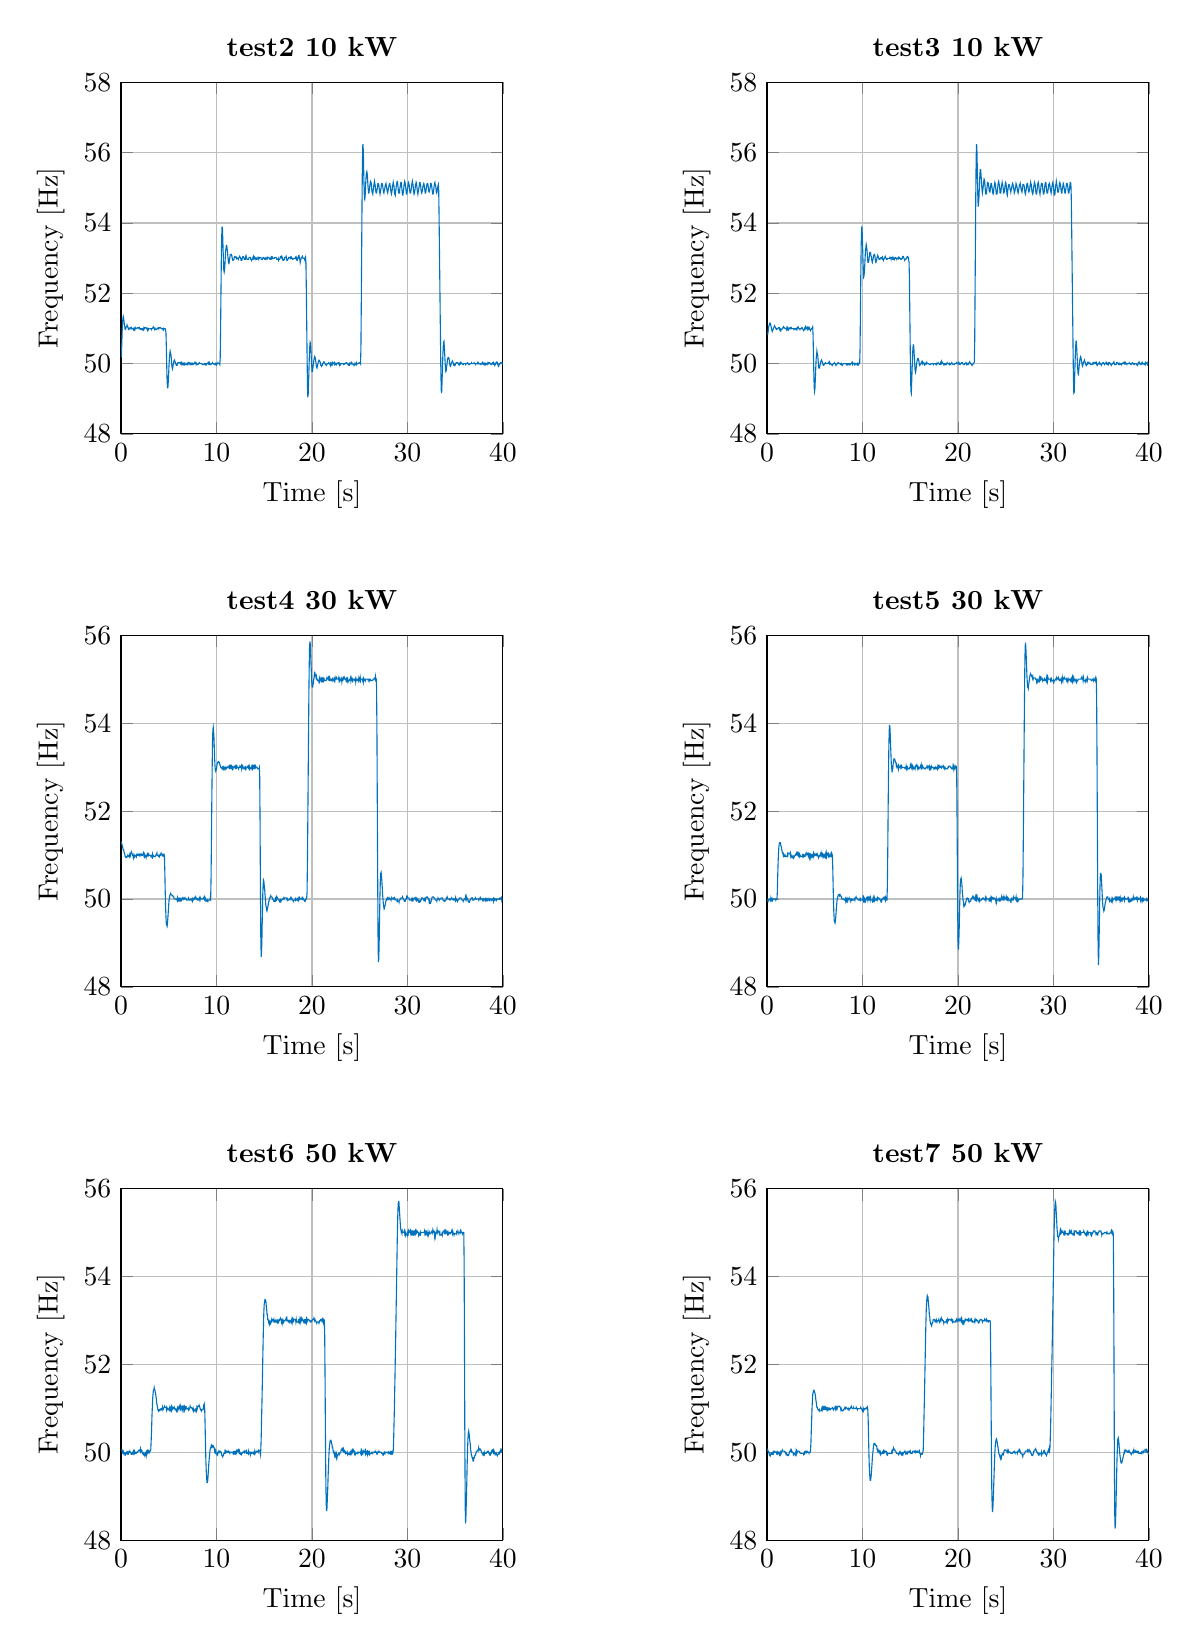
\begin{tikzpicture}

\begin{axis}[%
width=0.4\textwidth,
height=1.757in,
at={(0.953in,6.546in)},
scale only axis,
xmin=0,
xmax=40,
xlabel={Time [s]},
xmajorgrids,
ymin=48,
ymax=58,
ylabel={Frequency [Hz]},
ymajorgrids,
axis background/.style={fill=white},
title style={font=\bfseries},
title={test2 10 kW}
]
\addplot [color=mycolor1,solid,forget plot]
  table[row sep=crcr]{%
0.03986	50.1756146512795\\
0.07972	50.5561172901921\\
0.11928	50.9164969450102\\
0.15856	51.150895140665\\
0.19766	51.2820512820513\\
0.23666	51.3347022587269\\
0.27562	51.2820512820513\\
0.31462	51.2032770097286\\
0.35368	51.098620337251\\
0.39282	51.0464522715671\\
0.432	50.9683995922528\\
0.47124	50.9683995922528\\
0.51048	51.0204081632653\\
0.54968	51.0464522715671\\
0.58886	51.0464522715671\\
0.62804	51.0986203372508\\
0.66718	51.0725229826354\\
0.70634	51.0464522715671\\
0.74552	51.0204081632653\\
0.78472	50.9683995922529\\
0.82396	50.9683995922527\\
0.8632	50.9943906170322\\
0.90242	50.9943906170321\\
0.94164	51.0204081632653\\
0.98084	51.0204081632654\\
1.02004	51.0204081632651\\
1.05924	50.9943906170321\\
1.09846	51.0204081632654\\
1.13766	50.9943906170321\\
1.17688	50.9943906170321\\
1.2161	50.9943906170321\\
1.25532	50.9943906170324\\
1.29454	50.9683995922526\\
1.33378	50.9943906170324\\
1.373	50.9683995922526\\
1.41224	50.9943906170321\\
1.45146	50.9683995922529\\
1.4907	51.0204081632654\\
1.5299	50.9943906170321\\
1.56912	50.9943906170321\\
1.60834	50.9943906170321\\
1.64756	50.9943906170321\\
1.68678	51.0204081632654\\
1.72598	51.0204081632654\\
1.76518	51.0204081632651\\
1.80438	51.0204081632654\\
1.84358	51.0204081632651\\
1.88278	50.9943906170321\\
1.922	51.0204081632654\\
1.9612	50.9943906170324\\
2.00042	50.9943906170318\\
2.03964	50.9943906170324\\
2.07886	50.9683995922529\\
2.1181	50.9683995922529\\
2.15734	50.9943906170318\\
2.19656	50.9943906170324\\
2.23578	50.9683995922529\\
2.27502	50.9943906170318\\
2.31424	50.9943906170324\\
2.35346	50.9683995922529\\
2.3927	51.0204081632651\\
2.4319	50.9943906170318\\
2.47112	51.0204081632657\\
2.51032	51.0204081632651\\
2.54952	51.0204081632651\\
2.58872	51.0204081632657\\
2.62792	51.0204081632651\\
2.66712	50.9943906170318\\
2.70634	50.9943906170324\\
2.74556	50.9683995922529\\
2.7848	50.9424350483952\\
2.82406	50.9943906170324\\
2.86328	50.9683995922529\\
2.90252	50.9943906170318\\
2.94174	50.9943906170324\\
2.98096	50.9943906170318\\
3.02018	50.9943906170324\\
3.0594	50.9943906170318\\
3.09862	50.9943906170324\\
3.13784	50.9943906170324\\
3.17706	50.9683995922523\\
3.2163	50.9943906170324\\
3.25552	50.9943906170324\\
3.29474	50.9943906170318\\
3.33396	51.0204081632657\\
3.37316	51.0464522715671\\
3.41234	51.0204081632651\\
3.45154	51.0204081632651\\
3.49074	50.9943906170324\\
3.52996	50.9683995922529\\
3.5692	50.9943906170318\\
3.60842	50.9683995922529\\
3.64766	50.9683995922529\\
3.6869	50.9683995922529\\
3.72614	50.9683995922529\\
3.76538	50.9943906170318\\
3.8046	50.9943906170324\\
3.84382	50.9943906170318\\
3.88304	51.0204081632657\\
3.92224	51.0204081632651\\
3.96144	50.9943906170318\\
4.00066	51.0204081632651\\
4.03986	51.0204081632663\\
4.07906	51.0204081632651\\
4.11826	51.0204081632651\\
4.15746	51.0204081632651\\
4.19666	50.9943906170318\\
4.23588	50.9943906170329\\
4.2751	50.9943906170318\\
4.31432	50.9943906170318\\
4.35354	50.9943906170318\\
4.39276	50.9683995922535\\
4.432	50.9943906170318\\
4.47122	50.9683995922535\\
4.51046	50.9943906170318\\
4.54968	50.9943906170318\\
4.5889	50.9943906170318\\
4.62812	50.9943906170329\\
4.66734	50.9683995922523\\
4.70658	50.8646998982706\\
4.7459	50.4795557799089\\
4.78552	49.9500499500507\\
4.82556	49.5294700346708\\
4.86594	49.3096646942799\\
4.9065	49.3096646942799\\
4.94706	49.4804552201879\\
4.98748	49.7017892644137\\
5.02772	49.9500499500496\\
5.06776	50.150451354062\\
5.10764	50.2765208647568\\
5.14742	50.3524672708963\\
5.18714	50.3018108651908\\
5.2269	50.2512562814075\\
5.2667	50.150451354062\\
5.30658	49.9750124937529\\
5.3466	49.9001996007988\\
5.38668	49.850448654038\\
5.4268	49.9001996007977\\
5.46688	49.9750124937529\\
5.5069	50.0250125062532\\
5.54688	50.075112669004\\
5.58682	50.1002004008011\\
5.62674	50.075112669004\\
5.66668	50.0500500500503\\
5.70664	50\\
5.74664	50\\
5.78664	49.9500499500496\\
5.82668	49.9500499500507\\
5.86672	49.9500499500496\\
5.90676	50\\
5.94676	50.0250125062532\\
5.98674	50.0250125062532\\
6.02672	50.0250125062532\\
6.0667	50.0250125062521\\
6.10668	50.0250125062532\\
6.14666	50.0250125062532\\
6.18664	50.0250125062532\\
6.22662	50\\
6.26662	50.0250125062532\\
6.3066	50\\
6.3466	50.0250125062532\\
6.38658	49.9750124937529\\
6.4266	50\\
6.4666	49.9750124937529\\
6.50662	49.975012493754\\
6.54664	50\\
6.58664	49.9750124937529\\
6.62666	50\\
6.66666	49.9750124937529\\
6.70668	50\\
6.74668	49.9750124937529\\
6.7867	49.975012493754\\
6.82672	49.9750124937529\\
6.86674	49.9750124937529\\
6.90676	50\\
6.94676	49.9750124937529\\
6.98678	50\\
7.02678	50.0250125062532\\
7.06676	50\\
7.10676	50.0250125062532\\
7.14674	50.0250125062532\\
7.18672	50\\
7.22672	49.9750124937529\\
7.26674	50\\
7.30674	49.9750124937529\\
7.34676	49.975012493754\\
7.38678	50\\
7.42678	49.9750124937529\\
7.4668	49.9750124937529\\
7.50682	50\\
7.54682	49.9750124937529\\
7.58684	49.9750124937529\\
7.62686	50.0000000000011\\
7.66686	50\\
7.70686	50.0250125062521\\
7.74684	50\\
7.78684	50.0000000000011\\
7.82684	50.0250125062521\\
7.86682	49.975012493754\\
7.90684	50\\
7.94684	49.9750124937529\\
7.98686	49.975012493754\\
8.02688	49.9750124937529\\
8.0669	49.9750124937529\\
8.10692	49.9999999999988\\
8.14692	50.0000000000011\\
8.18692	50.0250125062532\\
8.2269	50.0250125062532\\
8.26688	49.9999999999988\\
8.30688	50.0000000000011\\
8.34688	49.9999999999988\\
8.38688	50.0000000000011\\
8.42688	49.9999999999988\\
8.46688	50.0000000000011\\
8.50688	49.9750124937529\\
8.5469	49.9750124937529\\
8.58692	49.9750124937529\\
8.62694	49.9750124937529\\
8.66696	49.9750124937529\\
8.70698	49.9750124937529\\
8.747	50.0000000000011\\
8.787	49.9999999999988\\
8.827	49.9750124937551\\
8.86702	49.9999999999988\\
8.90702	50.0000000000011\\
8.94702	49.9750124937529\\
8.98704	49.9999999999988\\
9.02704	50.0000000000011\\
9.06704	49.9999999999988\\
9.10704	50.0250125062532\\
9.14702	50.0000000000011\\
9.18702	50.0250125062532\\
9.227	49.9999999999988\\
9.267	50.0250125062532\\
9.30698	49.9750124937529\\
9.347	49.9750124937529\\
9.38702	49.9750124937529\\
9.42704	49.9750124937529\\
9.46706	50.0000000000011\\
9.50706	50.0000000000011\\
9.54706	49.9999999999988\\
9.58706	50.0250125062532\\
9.62704	50.0000000000011\\
9.66704	49.9999999999988\\
9.70704	50.0000000000011\\
9.74704	49.9750124937529\\
9.78706	49.9750124937529\\
9.82708	49.9750124937529\\
9.8671	49.9750124937529\\
9.90712	49.9999999999988\\
9.94712	49.9750124937551\\
9.98714	49.9999999999988\\
10.02714	49.9750124937529\\
10.06716	50.0000000000011\\
10.10716	49.9999999999988\\
10.14716	50.0250125062532\\
10.18714	50.0000000000011\\
10.22714	49.9999999999988\\
10.26714	50.0000000000011\\
10.30714	49.9999999999988\\
10.34714	49.9750124937529\\
10.38716	50.150451354062\\
10.42704	50.9164969450105\\
10.46632	51.9750519750522\\
10.5048	52.9661016949146\\
10.54256	53.5905680600224\\
10.57988	53.8793103448279\\
10.617	53.8793103448279\\
10.65412	53.5905680600224\\
10.69144	53.2481363152277\\
10.729	52.9100529100519\\
10.7668	52.6592943654566\\
10.80478	52.6038926880596\\
10.8428	52.6592943654541\\
10.88078	52.7983104540662\\
10.91866	53.022269353128\\
10.95638	53.191489361703\\
10.99398	53.2765050612681\\
11.03152	53.3617929562428\\
11.069	53.3617929562428\\
11.10648	53.2765050612681\\
11.14402	53.2197977647683\\
11.1816	53.0785562632697\\
11.21928	52.9661016949171\\
11.25704	52.8820729772608\\
11.29486	52.8541226215631\\
11.3327	52.8820729772608\\
11.37052	52.9941706412302\\
11.40826	53.022269353128\\
11.44598	53.1067445565577\\
11.48364	53.1067445565602\\
11.5213	53.1067445565577\\
11.55896	53.1067445565577\\
11.59662	53.0785562632697\\
11.6343	53.022269353128\\
11.67202	52.9661016949171\\
11.70978	52.9380624669141\\
11.74756	52.9380624669116\\
11.78534	52.9661016949171\\
11.8231	52.9661016949146\\
11.86086	53.022269353128\\
11.89858	53.0503978779852\\
11.93628	53.0503978779827\\
11.97398	53.022269353128\\
12.0117	53.022269353128\\
12.04942	53.022269353128\\
12.08714	52.9941706412302\\
12.12488	53.022269353128\\
12.1626	52.9941706412302\\
12.20034	52.9941706412302\\
12.23808	52.9941706412278\\
12.27582	52.9661016949171\\
12.31358	52.9941706412278\\
12.35132	53.022269353128\\
12.38904	53.0222693531305\\
12.42676	53.0503978779827\\
12.46446	53.022269353128\\
12.50218	53.022269353128\\
12.5399	52.9941706412302\\
12.57764	52.9380624669141\\
12.61542	52.9380624669141\\
12.6532	52.9380624669116\\
12.69098	52.9941706412302\\
12.72872	53.022269353128\\
12.76644	53.0503978779852\\
12.80414	53.0503978779827\\
12.84184	53.022269353128\\
12.87956	52.9941706412302\\
12.9173	52.9661016949146\\
12.95506	52.9661016949171\\
12.99282	52.9661016949146\\
13.03058	53.022269353128\\
13.0683	52.9941706412302\\
13.10604	53.0503978779827\\
13.14374	52.9941706412302\\
13.18148	52.9941706412302\\
13.21922	52.9661016949146\\
13.25698	52.9661016949146\\
13.29474	52.9661016949146\\
13.3325	52.9661016949171\\
13.37026	52.9661016949146\\
13.40802	53.022269353128\\
13.44574	53.022269353128\\
13.48346	53.022269353128\\
13.52118	53.022269353128\\
13.5589	53.0222693531305\\
13.59662	52.9661016949146\\
13.63438	52.9661016949146\\
13.67214	52.9380624669141\\
13.70992	52.9661016949146\\
13.74768	52.9661016949146\\
13.78544	52.9941706412302\\
13.82318	53.022269353128\\
13.8609	53.0503978779852\\
13.8986	52.9941706412278\\
13.93634	53.0222693531305\\
13.97406	52.9941706412278\\
14.0118	53.022269353128\\
14.04952	52.9941706412302\\
14.08726	52.9941706412302\\
14.125	52.9661016949146\\
14.16276	52.9941706412302\\
14.2005	52.9661016949146\\
14.23826	52.9661016949146\\
14.27602	52.9941706412302\\
14.31376	52.9941706412302\\
14.3515	53.022269353128\\
14.38922	52.9941706412278\\
14.42696	52.9661016949171\\
14.46472	52.9941706412278\\
14.50246	53.022269353128\\
14.54018	53.0222693531305\\
14.5779	53.022269353128\\
14.61562	53.022269353128\\
14.65334	53.022269353128\\
14.69106	52.9661016949146\\
14.72882	52.9661016949146\\
14.76658	52.9661016949171\\
14.80434	52.9661016949146\\
14.8421	52.9941706412302\\
14.87984	53.022269353128\\
14.91756	53.022269353128\\
14.95528	53.022269353128\\
14.993	52.9941706412302\\
15.03074	52.9941706412278\\
15.06848	52.9661016949171\\
15.10624	52.9661016949146\\
15.144	52.9941706412302\\
15.18174	52.9661016949146\\
15.2195	52.9941706412278\\
15.25724	52.9941706412302\\
15.29498	53.022269353128\\
15.3327	52.9941706412302\\
15.37044	53.022269353128\\
15.40816	53.022269353128\\
15.44588	53.022269353128\\
15.4836	53.022269353128\\
15.52132	52.9941706412302\\
15.55906	52.9941706412302\\
15.5968	52.9661016949146\\
15.63456	52.9661016949146\\
15.67232	52.9941706412302\\
15.71006	53.022269353128\\
15.74778	52.9941706412302\\
15.78552	53.022269353128\\
15.82324	52.9941706412302\\
15.86098	53.022269353128\\
15.8987	52.9941706412278\\
15.93644	52.9941706412302\\
15.97418	52.9941706412278\\
16.01192	52.9941706412302\\
16.04966	52.9941706412302\\
16.0874	53.022269353128\\
16.12512	53.022269353128\\
16.16284	53.022269353128\\
16.20056	53.022269353128\\
16.23828	53.022269353128\\
16.276	52.9941706412302\\
16.31374	52.9661016949171\\
16.3515	52.9661016949121\\
16.38926	52.9661016949171\\
16.42702	52.9661016949171\\
16.46478	52.9941706412302\\
16.50252	52.9380624669116\\
16.5403	52.9661016949171\\
16.57806	52.9661016949121\\
16.61582	52.9661016949171\\
16.65358	52.9941706412302\\
16.69132	53.0503978779827\\
16.72902	53.0503978779827\\
16.76672	53.0503978779877\\
16.80442	53.022269353128\\
16.84214	53.0503978779827\\
16.87984	53.022269353128\\
16.91756	52.9941706412302\\
16.9553	52.9380624669116\\
16.99308	52.9380624669166\\
17.03086	52.9380624669116\\
17.06864	52.9661016949171\\
17.1064	52.9661016949121\\
17.14416	53.022269353128\\
17.18188	53.022269353128\\
17.2196	53.022269353128\\
17.25732	53.022269353128\\
17.29504	53.0503978779877\\
17.33274	52.9941706412302\\
17.37048	52.9380624669116\\
17.40826	52.9380624669116\\
17.44604	52.9661016949171\\
17.4838	52.9661016949171\\
17.52156	52.9941706412302\\
17.5593	53.022269353128\\
17.59702	53.022269353128\\
17.63474	53.022269353128\\
17.67246	53.022269353128\\
17.71018	52.9941706412302\\
17.74792	53.022269353128\\
17.78564	52.9941706412302\\
17.82338	52.9941706412253\\
17.86112	53.022269353128\\
17.89884	52.9941706412302\\
17.93658	52.9941706412302\\
17.97432	52.9661016949171\\
18.01208	52.9661016949121\\
18.04984	52.9941706412302\\
18.08758	52.9941706412302\\
18.12532	52.9941706412302\\
18.16306	52.9941706412302\\
18.2008	52.9941706412302\\
18.23854	52.9941706412253\\
18.27628	53.022269353128\\
18.314	52.9941706412302\\
18.35174	53.022269353128\\
18.38946	52.9661016949171\\
18.42722	52.9380624669116\\
18.465	52.9380624669166\\
18.50278	52.9941706412302\\
18.54052	53.022269353128\\
18.57824	53.0503978779827\\
18.61594	53.022269353128\\
18.65366	53.0503978779827\\
18.69136	52.9941706412302\\
18.7291	52.9661016949171\\
18.76686	52.8820729772608\\
18.80468	52.9380624669116\\
18.84246	52.9661016949171\\
18.88022	53.022269353128\\
18.91794	53.022269353128\\
18.95566	53.022269353128\\
18.99338	53.0503978779827\\
19.03108	53.022269353128\\
19.0688	52.9941706412302\\
19.10654	52.9941706412302\\
19.14428	52.9941706412302\\
19.18202	52.9941706412302\\
19.21976	52.9661016949121\\
19.25752	52.9941706412302\\
19.29526	52.9380624669166\\
19.33304	52.9941706412253\\
19.37078	52.8541226215656\\
19.40862	52.1376433785181\\
19.44698	51.2295081967214\\
19.48602	50.2765208647602\\
19.5258	49.4071146245031\\
19.56628	49.0436488474766\\
19.60706	49.1400491400479\\
19.64776	49.5049504950473\\
19.68816	49.8504486540402\\
19.72828	50.2512562814075\\
19.76808	50.47955577991\\
19.8077	50.6072874493933\\
19.84722	50.5816894284239\\
19.88676	50.4032258064508\\
19.92644	50.1756146512828\\
19.9663	49.9750124937463\\
20.00632	49.776007964162\\
20.0465	49.776007964162\\
20.08668	49.8504486540358\\
20.1268	49.9500499500529\\
20.16684	50.0250125062532\\
20.20682	50.1253132832043\\
20.24672	50.1504513540665\\
20.2866	50.2008032128493\\
20.32644	50.1756146512784\\
20.3663	50.1253132832088\\
20.4062	50.0500500500492\\
20.44616	49.9500499500529\\
20.4862	49.9001996007944\\
20.52628	49.8753117206996\\
20.56638	49.9251123315022\\
20.60644	49.9750124937551\\
20.64646	50.0250125062532\\
20.68644	50.0500500500492\\
20.7264	50.1002004008033\\
20.76632	50.1002004007989\\
20.80624	50.0751126690062\\
20.84618	50.0500500500492\\
20.88614	50.0250125062532\\
20.92612	49.9500499500485\\
20.96616	49.9500499500485\\
21.0062	49.9251123315066\\
21.04626	49.9500499500485\\
21.0863	49.9500499500485\\
21.12634	50.0000000000011\\
21.16634	50.0000000000011\\
21.20634	50.0500500500492\\
21.2463	50.0500500500492\\
21.28626	50.0500500500492\\
21.32622	50.0250125062532\\
21.3662	50.0000000000011\\
21.4062	49.9750124937551\\
21.44622	49.9750124937507\\
21.48624	49.9500499500529\\
21.52628	49.9750124937507\\
21.5663	49.9750124937551\\
21.60632	49.9999999999966\\
21.64632	50.0000000000011\\
21.68632	50.0000000000011\\
21.72632	50.0000000000011\\
21.76632	50.0250125062532\\
21.8063	49.9999999999966\\
21.8463	50.0000000000011\\
21.8863	49.9750124937551\\
21.92632	49.9999999999966\\
21.96632	49.9500499500529\\
22.00636	50.0000000000011\\
22.04636	49.9750124937507\\
22.08638	50.0000000000011\\
22.12638	49.9750124937507\\
22.1664	50.0250125062532\\
22.20638	50.0000000000011\\
22.24638	50.0000000000011\\
22.28638	50.0000000000011\\
22.32638	50.0250125062532\\
22.36636	49.9750124937507\\
22.40638	50.0000000000011\\
22.44638	49.9750124937507\\
22.4864	49.9750124937551\\
22.52642	50.0000000000011\\
22.56642	49.9750124937507\\
22.60644	50.0000000000011\\
22.64644	50.0000000000011\\
22.68644	50.0000000000011\\
22.72644	50.0250125062532\\
22.76642	50.0250125062532\\
22.8064	49.9999999999966\\
22.8464	49.9750124937551\\
22.88642	50.0000000000011\\
22.92642	49.9500499500485\\
22.96646	49.9750124937551\\
23.00648	49.9750124937507\\
23.0465	50.0000000000011\\
23.0865	50.0000000000011\\
23.1265	49.9999999999966\\
23.1665	50.0000000000011\\
23.2065	50.0000000000011\\
23.2465	50.0000000000011\\
23.2865	49.9999999999966\\
23.3265	49.9750124937551\\
23.36652	49.9750124937551\\
23.40654	49.9999999999966\\
23.44654	50.0000000000011\\
23.48654	50.0000000000011\\
23.52654	50.0000000000011\\
23.56654	50.0250125062532\\
23.60652	50.0250125062488\\
23.6465	50.0250125062532\\
23.68648	50.0000000000011\\
23.72648	50.0000000000011\\
23.76648	49.9750124937551\\
23.8065	49.9750124937507\\
23.84652	49.9500499500485\\
23.88656	49.9500499500529\\
23.9266	50.0000000000011\\
23.9666	49.9750124937507\\
24.00662	50.0000000000011\\
24.04662	49.9999999999966\\
24.08662	50.0250125062532\\
24.1266	50.0000000000011\\
24.1666	50.0250125062532\\
24.20658	50.0000000000011\\
24.24658	50.0000000000011\\
24.28658	49.9750124937551\\
24.3266	49.9750124937507\\
24.36662	49.9750124937507\\
24.40664	49.9500499500529\\
24.44668	49.9750124937551\\
24.4867	49.9999999999966\\
24.5267	49.9750124937507\\
24.56672	50.0000000000011\\
24.60672	50.0000000000011\\
24.64672	50.0250125062532\\
24.6867	49.9750124937551\\
24.72672	50.0000000000011\\
24.76672	49.9999999999966\\
24.80672	50.0000000000011\\
24.84672	49.9999999999966\\
24.88672	50.0000000000011\\
24.92672	50.0250125062532\\
24.9667	50.0250125062532\\
25.00668	50.0250125062532\\
25.04666	50.0250125062532\\
25.08664	50.0000000000011\\
25.12664	50.4286434694935\\
25.1663	51.7063081695975\\
25.20498	53.1914893616954\\
25.24258	54.5851528384303\\
25.27922	55.6173526140166\\
25.31518	56.1797752809009\\
25.35078	56.242969628796\\
25.38634	55.9284116331099\\
25.4221	55.4323725055458\\
25.45818	55.0055005500521\\
25.49454	54.7045951859934\\
25.5311	54.6746856205566\\
25.56768	54.7645125958441\\
25.6042	54.9752611324886\\
25.64058	55.1876379690959\\
25.67682	55.3403431101224\\
25.71296	55.4323725055458\\
25.74904	55.4631170271783\\
25.7851	55.4016620498598\\
25.8212	55.2791597567746\\
25.85738	55.096418732776\\
25.89368	54.9752611324939\\
25.93006	54.8546352166732\\
25.96652	54.8546352166786\\
26.00298	54.9450549450543\\
26.03938	55.0055005500521\\
26.07574	55.0964187327868\\
26.11204	55.157198014343\\
26.1483	55.1876379690905\\
26.18454	55.157198014343\\
26.2208	55.0964187327814\\
26.2571	54.9752611324886\\
26.29348	54.884742041714\\
26.32992	54.8546352166786\\
26.36638	54.8245614035073\\
26.40286	54.914881932999\\
26.43928	54.9752611324939\\
26.47566	55.0660792951543\\
26.51198	55.1267916207309\\
26.54826	55.1876379690905\\
26.5845	55.1267916207255\\
26.62078	55.0660792951597\\
26.6571	54.9752611324886\\
26.69348	54.884742041714\\
26.72992	54.8546352166732\\
26.76638	54.8546352166732\\
26.80284	54.9450549450543\\
26.83924	54.9752611324939\\
26.87562	55.0660792951543\\
26.91194	55.1267916207309\\
26.94822	55.1267916207255\\
26.9845	55.0964187327814\\
27.0208	55.0357732526155\\
27.05714	54.9450549450543\\
27.09354	54.8847420417087\\
27.12998	54.8245614035127\\
27.16646	54.884742041714\\
27.2029	54.9450549450543\\
27.2393	55.0055005500521\\
27.27566	55.0964187327868\\
27.31196	55.1267916207255\\
27.34824	55.1267916207255\\
27.38452	55.0964187327868\\
27.42082	55.0357732526101\\
27.45716	54.9450549450543\\
27.49356	54.884742041714\\
27.53	54.8546352166786\\
27.56646	54.9148819330043\\
27.60288	54.9450549450543\\
27.63928	55.0055005500521\\
27.67564	55.0660792951543\\
27.71196	55.0964187327814\\
27.74826	55.1267916207309\\
27.78454	55.0660792951489\\
27.82086	55.0055005500574\\
27.85722	54.9450549450597\\
27.89362	54.8847420417087\\
27.93006	54.8546352166732\\
27.96652	54.9148819330043\\
28.00294	54.9752611324886\\
28.03932	55.0357732526209\\
28.07566	55.0660792951489\\
28.11198	55.1267916207309\\
28.14826	55.1267916207309\\
28.18454	55.0660792951489\\
28.22086	55.0357732526155\\
28.2572	54.9148819330043\\
28.29362	54.8546352166732\\
28.33008	54.8245614035127\\
28.36656	54.884742041714\\
28.403	54.9450549450543\\
28.4394	55.0660792951489\\
28.47572	55.0964187327868\\
28.51202	55.1571980143376\\
28.54828	55.0964187327814\\
28.58458	55.0660792951597\\
28.6209	54.9450549450543\\
28.6573	54.8245614035073\\
28.69378	54.8245614035073\\
28.73026	54.7945205479449\\
28.76676	54.9148819330043\\
28.80318	54.9752611324939\\
28.83956	55.0660792951489\\
28.87588	55.1267916207309\\
28.91216	55.1876379690959\\
28.9484	55.1876379690959\\
28.98464	55.096418732776\\
29.02094	55.0055005500574\\
29.0573	54.884742041714\\
29.09374	54.8546352166732\\
29.1302	54.8546352166786\\
29.16666	54.8546352166786\\
29.20312	54.9752611324886\\
29.2395	55.0357732526101\\
29.27584	55.1267916207309\\
29.31212	55.157198014343\\
29.34838	55.1571980143376\\
29.38464	55.0660792951543\\
29.42096	54.9752611324886\\
29.45734	54.8546352166786\\
29.4938	54.7945205479449\\
29.5303	54.7945205479449\\
29.5668	54.884742041714\\
29.60324	54.9450549450543\\
29.63964	55.0660792951489\\
29.67596	55.1267916207309\\
29.71224	55.1876379690959\\
29.74848	55.157198014343\\
29.78474	55.096418732776\\
29.82104	55.0055005500628\\
29.8574	54.914881932999\\
29.89382	54.8245614035073\\
29.9303	54.8245614035127\\
29.96678	54.884742041714\\
30.00322	54.9752611324886\\
30.0396	55.0357732526101\\
30.07594	55.1267916207309\\
30.11222	55.157198014343\\
30.14848	55.1267916207255\\
30.18476	55.0660792951543\\
30.22108	54.9752611324886\\
30.25746	54.884742041714\\
30.2939	54.8546352166786\\
30.33036	54.8546352166732\\
30.36682	54.9148819330043\\
30.40324	54.9752611324886\\
30.43962	55.0660792951543\\
30.47594	55.1267916207309\\
30.51222	55.1876379690959\\
30.54846	55.1267916207255\\
30.58474	55.0964187327814\\
30.62104	54.9752611324886\\
30.65742	54.884742041714\\
30.69386	54.8245614035127\\
30.73034	54.8546352166732\\
30.7668	54.914881932999\\
30.80322	54.9752611324939\\
30.8396	55.0964187327814\\
30.8759	55.0964187327868\\
30.9122	55.1571980143376\\
30.94846	55.1267916207255\\
30.98474	55.0357732526155\\
31.02108	54.9450549450597\\
31.05748	54.8847420417087\\
31.09392	54.8245614035073\\
31.1304	54.884742041714\\
31.16684	54.9450549450543\\
31.20324	55.0055005500521\\
31.2396	55.0660792951597\\
31.27592	55.1571980143376\\
31.31218	55.157198014343\\
31.34844	55.0964187327814\\
31.38474	55.0660792951543\\
31.42106	54.9450549450543\\
31.45746	54.884742041714\\
31.4939	54.8546352166732\\
31.53036	54.884742041714\\
31.5668	54.9148819330043\\
31.60322	55.0055005500521\\
31.63958	55.0660792951597\\
31.6759	55.096418732776\\
31.7122	55.1267916207309\\
31.74848	55.0964187327814\\
31.78478	55.0055005500574\\
31.82114	54.9450549450543\\
31.85754	54.8546352166786\\
31.894	54.8546352166732\\
31.93046	54.8847420417087\\
31.9669	54.9752611324886\\
32.00328	55.0357732526209\\
32.03962	55.096418732776\\
32.07592	55.1267916207309\\
32.1122	55.1267916207309\\
32.14848	55.096418732776\\
32.18478	55.0055005500628\\
32.22114	54.9148819330043\\
32.25756	54.884742041714\\
32.294	54.8847420417033\\
32.33044	54.9450549450543\\
32.36684	55.0055005500628\\
32.4032	55.0357732526101\\
32.43954	55.1267916207309\\
32.47582	55.1267916207201\\
32.5121	55.0964187327868\\
32.5484	55.0357732526101\\
32.58474	54.945054945065\\
32.62114	54.8847420417033\\
32.65758	54.8245614035127\\
32.69406	54.8245614035127\\
32.73054	54.9148819330043\\
32.76696	54.9752611324886\\
32.80334	55.0660792951489\\
32.83966	55.1267916207309\\
32.87594	55.157198014343\\
32.9122	55.096418732776\\
32.9485	55.0660792951597\\
32.98482	55.0055005500521\\
33.02118	54.884742041714\\
33.05762	54.8546352166786\\
33.09408	54.8847420417033\\
33.13052	54.945054945065\\
33.16692	55.0055005500521\\
33.20328	55.0660792951489\\
33.2396	55.0964187327868\\
33.2759	54.9148819330043\\
33.31232	54.2299349240728\\
33.3492	53.3333333333414\\
33.3867	52.4658971668426\\
33.42482	51.519835136526\\
33.46364	50.6329113924001\\
33.50314	49.701789264417\\
33.54338	49.2368291481979\\
33.584	49.1642084562502\\
33.62468	49.4804552201824\\
33.6651	49.8256103637258\\
33.70524	50.2008032128538\\
33.74508	50.4540867810311\\
33.78472	50.6072874493887\\
33.82424	50.6329113924092\\
33.86374	50.47955577991\\
33.90336	50.2765208647557\\
33.94314	50.0500500500492\\
33.9831	49.8504486540358\\
34.02322	49.776007964162\\
34.0634	49.8007968127488\\
34.10356	49.9251123315066\\
34.14362	49.9750124937551\\
34.18364	50.1002004007989\\
34.22356	50.1504513540575\\
34.26344	50.1756146512828\\
34.3033	50.1756146512828\\
34.34316	50.1504513540575\\
34.38304	50.1002004007989\\
34.42296	50.0000000000011\\
34.46296	49.9500499500529\\
34.503	49.9251123315066\\
34.54306	49.950049950044\\
34.5831	50.0000000000011\\
34.6231	50.0250125062532\\
34.66308	50.0500500500492\\
34.70304	50.0751126690017\\
34.74298	50.0500500500492\\
34.78294	50.0250125062532\\
34.82292	50.0000000000011\\
34.86292	49.9500499500529\\
34.90296	49.9500499500529\\
34.943	49.9750124937463\\
34.98302	49.9500499500529\\
35.02306	49.9750124937551\\
35.06308	50.0000000000011\\
35.10308	50.0250125062532\\
35.14306	50.0250125062532\\
35.18304	50.0250125062532\\
35.22302	50.0250125062532\\
35.263	50.0250125062532\\
35.30298	50.0000000000011\\
35.34298	49.9999999999922\\
35.38298	49.9750124937551\\
35.423	50.0000000000011\\
35.463	49.9750124937551\\
35.50302	50.0000000000011\\
35.54302	50.0250125062532\\
35.583	50.0000000000011\\
35.623	50.0250125062532\\
35.66298	50.0000000000011\\
35.70298	49.9999999999922\\
35.74298	50.0000000000011\\
35.78298	49.9750124937551\\
35.823	49.9750124937551\\
35.86302	49.9750124937463\\
35.90304	50.0000000000011\\
35.94304	50.0000000000011\\
35.98304	50.0000000000011\\
36.02304	50.0000000000011\\
36.06304	50.0000000000011\\
36.10304	49.9750124937551\\
36.14306	50.0000000000011\\
36.18306	49.9999999999922\\
36.22306	50.0000000000011\\
36.26306	50.0250125062532\\
36.30304	50.0250125062532\\
36.34302	50.0000000000011\\
36.38302	49.9750124937551\\
36.42304	49.9750124937551\\
36.46306	49.9750124937551\\
36.50308	49.9750124937463\\
36.5431	50.0000000000011\\
36.5831	50.0000000000011\\
36.6231	50.0000000000011\\
36.6631	50.0000000000011\\
36.7031	50.0250125062532\\
36.74308	50.0000000000011\\
36.78308	50.0000000000011\\
36.82308	50.0000000000011\\
36.86308	49.9999999999922\\
36.90308	50.0000000000011\\
36.94308	50.0000000000011\\
36.98308	50.0250125062532\\
37.02306	50.0000000000011\\
37.06306	50.0000000000011\\
37.10306	50.0000000000011\\
37.14306	49.9750124937463\\
37.18308	50.0000000000011\\
37.22308	50.0000000000011\\
37.26308	50.0000000000011\\
37.30308	50.0000000000011\\
37.34308	50.0250125062532\\
37.38306	50.0000000000011\\
37.42306	50.0250125062532\\
37.46304	50.0000000000011\\
37.50304	50.0000000000011\\
37.54304	50.0000000000011\\
37.58304	49.9999999999922\\
37.62304	49.9750124937551\\
37.66306	49.9750124937551\\
37.70308	49.9750124937551\\
37.7431	50.0000000000011\\
37.7831	50.0000000000011\\
37.8231	50.0250125062532\\
37.86308	49.9999999999922\\
37.90308	50.0250125062532\\
37.94306	50.0000000000011\\
37.98306	49.9750124937551\\
38.02308	49.9750124937551\\
38.0631	50.0000000000011\\
38.1031	49.9750124937463\\
38.14312	50.0000000000011\\
38.18312	49.9750124937551\\
38.22314	50.0000000000011\\
38.26314	50.0000000000011\\
38.30314	50.0000000000011\\
38.34314	49.9750124937463\\
38.38316	50.0000000000011\\
38.42316	50.0250125062532\\
38.46314	50.0000000000011\\
38.50314	50.0250125062532\\
38.54312	50.0250125062532\\
38.5831	50.0250125062532\\
38.62308	50.0250125062532\\
38.66306	50.0000000000011\\
38.70306	50.0000000000011\\
38.74306	49.9750124937551\\
38.78308	49.9750124937551\\
38.8231	49.9750124937463\\
38.86312	50.0000000000011\\
38.90312	50.0250125062532\\
38.9431	50.0250125062532\\
38.98308	50.0000000000011\\
39.02308	50.0250125062532\\
39.06306	49.9750124937551\\
39.10308	49.9750124937551\\
39.1431	49.950049950044\\
39.18314	49.9750124937551\\
39.22316	49.9750124937551\\
39.26318	50.0250125062532\\
39.30316	50.0250125062532\\
39.34314	50.0500500500492\\
39.3831	50.0500500500492\\
39.42306	50.0250125062532\\
39.46304	49.9750124937551\\
39.50306	49.950049950044\\
39.5431	49.9251123315066\\
39.58316	49.9500499500529\\
39.6232	49.9750124937463\\
39.66322	50.0000000000011\\
39.70322	50.0000000000011\\
39.74322	50.0250125062532\\
39.7832	50.0250125062532\\
39.82318	50.0250125062532\\
39.86316	50.0250125062532\\
39.90314	50.0250125062532\\
39.94312	49.9750124937551\\
};
\end{axis}

\begin{axis}[%
width=0.4\textwidth,
height=1.757in,
at={(4.183in,6.546in)},
scale only axis,
xmin=0,
xmax=40,
xlabel={Time [s]},
xmajorgrids,
ymin=48,
ymax=58,
ylabel={Frequency [Hz]},
ymajorgrids,
axis background/.style={fill=white},
title style={font=\bfseries},
title={test3 10 kW}
]
\addplot [color=mycolor1,solid,forget plot]
  table[row sep=crcr]{%
0.03908	50.8388408744281\\
0.07842	50.8388408744281\\
0.11776	50.9164969450102\\
0.15704	51.0204081632653\\
0.19624	51.0725229826353\\
0.2354	51.0986203372509\\
0.27454	51.1508951406649\\
0.31364	51.150895140665\\
0.35274	51.1508951406649\\
0.39184	51.0986203372509\\
0.43098	51.0464522715671\\
0.47016	50.9943906170322\\
0.50938	50.9424350483954\\
0.54864	50.9164969450101\\
0.58792	50.9424350483954\\
0.62718	50.9683995922529\\
0.66642	50.9943906170321\\
0.70564	51.0204081632653\\
0.74484	51.0464522715671\\
0.78402	51.0725229826354\\
0.82318	51.0464522715671\\
0.86236	51.0464522715671\\
0.90154	51.0204081632653\\
0.94074	50.9943906170321\\
0.97996	50.9683995922529\\
1.0192	50.9683995922529\\
1.05844	50.9943906170321\\
1.09766	50.9943906170321\\
1.13688	50.9943906170321\\
1.1761	51.0204081632654\\
1.2153	51.0204081632651\\
1.2545	51.0204081632654\\
1.2937	51.0204081632651\\
1.3329	50.9683995922529\\
1.37214	50.9424350483955\\
1.4114	50.9683995922526\\
1.45064	50.9424350483955\\
1.4899	50.9683995922526\\
1.52914	50.9683995922529\\
1.56838	50.9943906170321\\
1.6076	50.9943906170321\\
1.64682	51.0204081632654\\
1.68602	51.0204081632654\\
1.72522	51.0464522715671\\
1.7644	51.0204081632651\\
1.8036	51.0204081632654\\
1.8428	51.0204081632651\\
1.882	50.9943906170321\\
1.92122	50.9943906170324\\
1.96044	50.9943906170321\\
1.99966	50.9943906170321\\
2.03888	50.9683995922529\\
2.07812	51.0204081632651\\
2.11732	50.9943906170324\\
2.15654	51.0204081632651\\
2.19574	50.9683995922529\\
2.23498	50.9943906170318\\
2.2742	50.9683995922529\\
2.31344	50.9943906170324\\
2.35266	50.9943906170318\\
2.39188	51.0204081632657\\
2.43108	51.0204081632651\\
2.47028	51.0204081632651\\
2.50948	50.9943906170324\\
2.5487	51.0204081632651\\
2.5879	50.9943906170324\\
2.62712	50.9943906170318\\
2.66634	50.9943906170324\\
2.70556	50.9943906170324\\
2.74478	50.9943906170318\\
2.784	50.9943906170324\\
2.82322	50.9683995922529\\
2.86246	50.9943906170318\\
2.90168	50.9943906170324\\
2.9409	50.9943906170318\\
2.98012	50.9943906170324\\
3.01934	50.9683995922529\\
3.05858	50.9683995922529\\
3.09782	50.9943906170318\\
3.13704	50.9683995922529\\
3.17628	51.0204081632651\\
3.21548	51.0204081632657\\
3.25468	51.0464522715671\\
3.29386	51.0204081632651\\
3.33306	50.9943906170324\\
3.37228	50.9943906170318\\
3.4115	50.9943906170324\\
3.45072	50.9683995922529\\
3.48996	50.9943906170318\\
3.52918	50.9943906170324\\
3.5684	50.9943906170318\\
3.60762	50.9943906170324\\
3.64684	51.0204081632651\\
3.68604	51.0204081632651\\
3.72524	50.9943906170324\\
3.76446	50.9683995922529\\
3.8037	50.9683995922529\\
3.84294	50.9424350483952\\
3.8822	50.9683995922529\\
3.92144	50.9683995922529\\
3.96068	51.0204081632651\\
3.99988	51.0204081632657\\
4.03908	51.0464522715671\\
4.07826	50.9943906170318\\
4.11748	51.0204081632651\\
4.15668	50.9943906170318\\
4.1959	50.9943906170329\\
4.23512	51.0204081632651\\
4.27432	50.9683995922523\\
4.31356	50.9943906170329\\
4.35278	51.0204081632651\\
4.39198	50.9943906170318\\
4.4312	51.0204081632651\\
4.4704	50.9943906170318\\
4.50962	50.9683995922535\\
4.54886	50.9424350483946\\
4.58812	50.9683995922535\\
4.62736	50.9683995922523\\
4.6666	50.9943906170329\\
4.70582	50.9943906170318\\
4.74504	51.0204081632651\\
4.78424	51.0464522715671\\
4.82342	50.8130081300809\\
4.86278	50.2765208647568\\
4.90256	49.7265042267521\\
4.94278	49.309664694281\\
4.98334	49.212598425196\\
5.02398	49.309664694281\\
5.06454	49.6031746031742\\
5.10486	49.8753117206985\\
5.14496	50.1253132832077\\
5.18486	50.2260170768461\\
5.22468	50.3524672708963\\
5.2644	50.2765208647557\\
5.30418	50.2512562814075\\
5.34398	50.1253132832077\\
5.38388	49.9750124937529\\
5.4239	49.8753117206985\\
5.464	49.8753117206985\\
5.5041	49.8753117206985\\
5.5442	49.9500499500496\\
5.58424	50\\
5.62424	50.0500500500503\\
5.6642	50.0751126690028\\
5.70414	50.1002004008022\\
5.74406	50.0751126690028\\
5.784	50.0500500500503\\
5.82396	50.0250125062532\\
5.86394	49.9750124937529\\
5.90396	49.9500499500507\\
5.944	49.9500499500496\\
5.98404	49.9750124937529\\
6.02406	50\\
6.06406	50\\
6.10406	50.0250125062532\\
6.14404	50.0250125062532\\
6.18402	50\\
6.22402	50\\
6.26402	50\\
6.30402	50\\
6.34402	50\\
6.38402	50\\
6.42402	50.0250125062532\\
6.464	50.0250125062532\\
6.50398	50.0500500500503\\
6.54394	50\\
6.58394	50.0250125062532\\
6.62392	50\\
6.66392	50\\
6.70392	49.9750124937529\\
6.74394	49.9750124937529\\
6.78396	49.9750124937529\\
6.82398	49.9500499500507\\
6.86402	49.9750124937529\\
6.90404	49.9750124937529\\
6.94406	50\\
6.98406	50\\
7.02406	50\\
7.06406	50.0250125062532\\
7.10404	50\\
7.14404	50\\
7.18404	49.9750124937529\\
7.22406	49.9500499500507\\
7.2641	49.9750124937529\\
7.30412	49.9750124937529\\
7.34414	50\\
7.38414	50\\
7.42414	50.0250125062532\\
7.46412	50.0250125062532\\
7.5041	50.0250125062532\\
7.54408	50\\
7.58408	50\\
7.62408	50\\
7.66408	50\\
7.70408	49.9750124937529\\
7.7441	49.9750124937529\\
7.78412	50\\
7.82412	49.975012493754\\
7.86414	49.9500499500496\\
7.90418	49.9750124937529\\
7.9442	49.9750124937529\\
7.98422	50\\
8.02422	50.0000000000011\\
8.06422	49.9999999999988\\
8.10422	50.0000000000011\\
8.14422	49.9999999999988\\
8.18422	50.0000000000011\\
8.22422	49.9999999999988\\
8.26422	50.0000000000011\\
8.30422	49.9750124937529\\
8.34424	49.9999999999988\\
8.38424	50.0000000000011\\
8.42424	49.9750124937529\\
8.46426	50.0000000000011\\
8.50426	49.9999999999988\\
8.54426	50.0000000000011\\
8.58426	49.9750124937529\\
8.62428	49.9999999999988\\
8.66428	50.0000000000011\\
8.70428	49.9750124937529\\
8.7443	49.9999999999988\\
8.7843	50.0000000000011\\
8.8243	49.9999999999988\\
8.8643	50.0250125062532\\
8.90428	50.0000000000011\\
8.94428	49.9750124937529\\
8.9843	50.0250125062532\\
9.02428	50.0000000000011\\
9.06428	49.9999999999988\\
9.10428	50.0000000000011\\
9.14428	49.9750124937529\\
9.1843	49.9999999999988\\
9.2243	49.9750124937529\\
9.26432	50.0000000000011\\
9.30432	49.9999999999988\\
9.34432	50.0000000000011\\
9.38432	49.9999999999988\\
9.42432	49.9750124937529\\
9.46434	50.0000000000011\\
9.50434	49.9750124937529\\
9.54436	50.0000000000011\\
9.58436	49.9750124937529\\
9.62438	49.9999999999988\\
9.66438	50.0000000000011\\
9.70438	49.9999999999988\\
9.74438	50.4032258064531\\
9.78406	51.4138817480721\\
9.82296	52.5210084033603\\
9.86104	53.3333333333338\\
9.89854	53.7634408602146\\
9.93574	53.9083557951474\\
9.97284	53.7056928034389\\
10.01008	53.3617929562428\\
10.04756	52.9941706412302\\
10.0853	52.6592943654541\\
10.12328	52.4658971668426\\
10.1614	52.4934383202099\\
10.1995	52.6315789473681\\
10.2375	52.7983104540662\\
10.27538	53.022269353128\\
10.3131	53.2197977647683\\
10.35068	53.3049040511718\\
10.3882	53.3902829685006\\
10.42566	53.3333333333338\\
10.46316	53.2481363152277\\
10.50072	53.1349628055265\\
10.53836	52.9661016949146\\
10.57612	52.8820729772608\\
10.61394	52.8820729772608\\
10.65176	52.9100529100544\\
10.68956	52.9941706412278\\
10.7273	53.0785562632697\\
10.76498	53.1632110579498\\
10.8026	53.1632110579473\\
10.84022	53.1632110579473\\
10.87784	53.0785562632697\\
10.91552	53.0503978779852\\
10.95322	52.9941706412278\\
10.99096	52.9100529100544\\
11.02876	52.8820729772608\\
11.06658	52.9380624669116\\
11.10436	52.9661016949171\\
11.14212	53.0503978779827\\
11.17982	53.0785562632697\\
11.2175	53.1067445565602\\
11.25516	53.1067445565577\\
11.29282	53.0785562632697\\
11.3305	52.9941706412302\\
11.36824	52.9100529100519\\
11.40604	52.8820729772608\\
11.44386	52.9100529100519\\
11.48166	52.9380624669141\\
11.51944	53.022269353128\\
11.55716	53.022269353128\\
11.59488	53.0785562632697\\
11.63256	53.0503978779852\\
11.67026	53.022269353128\\
11.70798	52.9941706412302\\
11.74572	52.9661016949146\\
11.78348	52.9661016949146\\
11.82124	52.9661016949171\\
11.859	52.9941706412278\\
11.89674	52.9941706412302\\
11.93448	53.022269353128\\
11.9722	53.022269353128\\
12.00992	53.022269353128\\
12.04764	52.9941706412302\\
12.08538	53.022269353128\\
12.1231	52.9661016949146\\
12.16086	52.9661016949171\\
12.19862	52.9380624669116\\
12.2364	52.9661016949171\\
12.27416	52.9941706412278\\
12.3119	53.0222693531305\\
12.34962	53.022269353128\\
12.38734	53.0503978779827\\
12.42504	53.022269353128\\
12.46276	52.9941706412302\\
12.5005	52.9661016949146\\
12.53826	52.9661016949146\\
12.57602	52.9661016949171\\
12.61378	52.9941706412278\\
12.65152	52.9941706412302\\
12.68926	52.9941706412302\\
12.727	52.9941706412278\\
12.76474	52.9941706412302\\
12.80248	52.9941706412302\\
12.84022	52.9941706412302\\
12.87796	53.022269353128\\
12.91568	52.9941706412278\\
12.95342	52.9941706412302\\
12.99116	52.9661016949146\\
13.02892	53.022269353128\\
13.06664	53.0222693531305\\
13.10436	53.022269353128\\
13.14208	52.9941706412278\\
13.17982	53.022269353128\\
13.21754	52.9661016949171\\
13.2553	52.9661016949146\\
13.29306	52.9941706412302\\
13.3308	52.9661016949146\\
13.36856	52.9941706412302\\
13.4063	52.9941706412278\\
13.44404	53.022269353128\\
13.48176	53.0222693531305\\
13.51948	52.9941706412278\\
13.55722	52.9941706412302\\
13.59496	52.9661016949146\\
13.63272	52.9941706412302\\
13.67046	52.9941706412302\\
13.7082	52.9941706412278\\
13.74594	53.022269353128\\
13.78366	52.9941706412302\\
13.8214	53.022269353128\\
13.85912	53.022269353128\\
13.89684	52.9941706412302\\
13.93458	52.9941706412302\\
13.97232	52.9941706412278\\
14.01006	52.9661016949171\\
14.04782	52.9661016949146\\
14.08558	52.9661016949146\\
14.12334	52.9941706412302\\
14.16108	52.9941706412278\\
14.19882	53.0503978779852\\
14.23652	53.0503978779852\\
14.27422	53.0503978779827\\
14.31192	53.022269353128\\
14.34964	52.9941706412302\\
14.38738	52.9661016949146\\
14.42514	52.9380624669141\\
14.46292	52.9661016949146\\
14.50068	52.9661016949146\\
14.53844	52.9661016949171\\
14.5762	52.9941706412278\\
14.61394	52.9941706412302\\
14.65168	53.022269353128\\
14.6894	53.0503978779852\\
14.7271	53.0503978779827\\
14.7648	53.022269353128\\
14.80252	53.0222693531305\\
14.84024	52.9380624669116\\
14.87802	52.8820729772608\\
14.91584	52.4109014675059\\
14.954	51.5198351365283\\
14.99282	50.6072874493933\\
15.03234	49.7017892644126\\
15.07258	49.2125984251971\\
15.11322	49.1642084562438\\
15.1539	49.4804552201868\\
15.19432	49.800796812751\\
15.23448	50.150451354062\\
15.27436	50.4032258064508\\
15.31404	50.5305709954512\\
15.35362	50.5305709954534\\
15.3932	50.3778337531488\\
15.4329	50.1756146512784\\
15.47276	49.9750124937529\\
15.51278	49.800796812751\\
15.55294	49.751243781094\\
15.59314	49.8007968127488\\
15.6333	49.9001996007988\\
15.67338	49.9999999999988\\
15.71338	50.075112669004\\
15.75332	50.1253132832088\\
15.79322	50.150451354062\\
15.8331	50.150451354062\\
15.87298	50.1002004008011\\
15.9129	50.075112669004\\
15.95284	49.9750124937529\\
15.99286	49.9500499500507\\
16.0329	49.9750124937507\\
16.07292	49.9750124937551\\
16.11294	50.0000000000011\\
16.15294	50.0250125062532\\
16.19292	50.0500500500492\\
16.23288	50.0250125062532\\
16.27286	50.0500500500492\\
16.31282	50.0000000000011\\
16.35282	50.0250125062532\\
16.3928	49.9999999999966\\
16.4328	50.0000000000011\\
16.4728	49.9750124937551\\
16.51282	50.0000000000011\\
16.55282	49.9750124937507\\
16.59284	50.0000000000011\\
16.63284	50.0000000000011\\
16.67284	50.0250125062532\\
16.71282	49.9999999999966\\
16.75282	50.0250125062532\\
16.7928	50.0000000000011\\
16.8328	50.0000000000011\\
16.8728	50.0000000000011\\
16.9128	49.9999999999966\\
16.9528	50.0000000000011\\
16.9928	49.9750124937551\\
17.03282	49.9750124937507\\
17.07284	49.9750124937551\\
17.11286	49.9750124937507\\
17.15288	49.9750124937551\\
17.1929	50.0000000000011\\
17.2329	49.9999999999966\\
17.2729	50.0000000000011\\
17.3129	50.0000000000011\\
17.3529	50.0000000000011\\
17.3929	49.9999999999966\\
17.4329	49.9750124937551\\
17.47292	50.0000000000011\\
17.51292	50.0000000000011\\
17.55292	49.9999999999966\\
17.59292	50.0000000000011\\
17.63292	50.0000000000011\\
17.67292	49.9750124937507\\
17.71294	49.9750124937551\\
17.75296	50.0000000000011\\
17.79296	49.9750124937507\\
17.83298	50.0000000000011\\
17.87298	50.0000000000011\\
17.91298	50.0250125062532\\
17.95296	49.9999999999966\\
17.99296	50.0000000000011\\
18.03296	50.0000000000011\\
18.07296	49.9750124937551\\
18.11298	49.9750124937507\\
18.153	49.9750124937551\\
18.19302	50.0250125062532\\
18.233	49.9999999999966\\
18.273	50.0500500500537\\
18.31296	49.9999999999966\\
18.35296	50.0000000000011\\
18.39296	50.0250125062532\\
18.43294	50.0000000000011\\
18.47294	50.0000000000011\\
18.51294	49.9750124937507\\
18.55296	50.0000000000011\\
18.59296	50.0000000000011\\
18.63296	49.9750124937507\\
18.67298	50.0000000000011\\
18.71298	50.0000000000011\\
18.75298	49.9750124937507\\
18.793	50.0000000000011\\
18.833	50.0000000000011\\
18.873	50.0250125062532\\
18.91298	50.0000000000011\\
18.95298	49.9999999999966\\
18.99298	50.0000000000011\\
19.03298	50.0000000000011\\
19.07298	49.9750124937507\\
19.113	50.0000000000011\\
19.153	49.9750124937551\\
19.19302	49.9750124937507\\
19.23304	49.9750124937551\\
19.27306	50.0000000000011\\
19.31306	49.9999999999966\\
19.35306	50.0250125062532\\
19.39304	50.0000000000011\\
19.43304	50.0000000000011\\
19.47304	49.9750124937507\\
19.51306	49.9750124937551\\
19.55308	49.9750124937507\\
19.5931	49.9750124937551\\
19.63312	49.9750124937551\\
19.67314	49.9999999999966\\
19.71314	50.0000000000011\\
19.75314	50.0000000000011\\
19.79314	50.0000000000011\\
19.83314	50.0250125062532\\
19.87312	49.9999999999966\\
19.91312	50.0000000000011\\
19.95312	50.0000000000011\\
19.99312	49.9999999999966\\
20.03312	50.0250125062532\\
20.0731	49.9999999999966\\
20.1131	50.0250125062532\\
20.15308	50.0000000000011\\
20.19308	49.9750124937551\\
20.2331	49.9750124937507\\
20.27312	50.0000000000011\\
20.31312	50.0000000000011\\
20.35312	50.0250125062532\\
20.3931	50.0250125062532\\
20.43308	50.0250125062532\\
20.47306	50.0250125062532\\
20.51304	49.9999999999966\\
20.55304	49.9750124937551\\
20.59306	49.9750124937507\\
20.63308	49.9750124937551\\
20.6731	49.9750124937551\\
20.71312	49.9999999999966\\
20.75312	50.0000000000011\\
20.79312	50.0000000000011\\
20.83312	50.0250125062532\\
20.8731	50.0000000000011\\
20.9131	49.9750124937507\\
20.95312	50.0000000000011\\
20.99312	49.9750124937507\\
21.03314	49.9750124937551\\
21.07316	49.9750124937507\\
21.11318	50.0000000000011\\
21.15318	50.0250125062532\\
21.19316	50.0250125062532\\
21.23314	50.0500500500492\\
21.2731	50.0250125062532\\
21.31308	50.0000000000011\\
21.35308	50.0000000000011\\
21.39308	49.9750124937507\\
21.4331	49.9750124937551\\
21.47312	49.9500499500485\\
21.51316	49.9750124937551\\
21.55318	49.9750124937507\\
21.5932	50.0000000000011\\
21.6332	50.0000000000011\\
21.6732	50.0250125062532\\
21.71318	50.0500500500492\\
21.75314	50.6329113924047\\
21.79264	52.0291363163401\\
21.83108	53.5331905781539\\
21.86844	54.884742041714\\
21.90488	55.8035714285709\\
21.94072	56.242969628796\\
21.97628	56.1797752809009\\
22.01188	55.741360089188\\
22.04776	55.1571980143376\\
22.08402	54.7045951859987\\
22.12058	54.4662309368154\\
22.1573	54.5851528384303\\
22.19394	54.7045951859934\\
22.2305	54.9450549450543\\
22.2669	55.1876379690959\\
22.30314	55.4323725055458\\
22.33922	55.5247084952795\\
22.37524	55.5247084952795\\
22.41126	55.4016620498598\\
22.44736	55.2486187845344\\
22.48356	55.0660792951543\\
22.51988	54.9450549450543\\
22.55628	54.8546352166732\\
22.59274	54.9148819330043\\
22.62916	55.0055005500574\\
22.66552	55.0964187327814\\
22.70182	55.1876379690959\\
22.73806	55.248618784529\\
22.77426	55.2181115405851\\
22.81048	55.157198014343\\
22.84674	55.0055005500521\\
22.8831	54.884742041714\\
22.91954	54.8245614035073\\
22.95602	54.8245614035127\\
22.9925	54.8847420417087\\
23.02894	54.9752611324939\\
23.06532	55.0660792951543\\
23.10164	55.1571980143376\\
23.1379	55.157198014343\\
23.17416	55.1267916207255\\
23.21044	55.0660792951543\\
23.24676	55.0055005500574\\
23.28312	54.9148819330043\\
23.31954	54.8847420417087\\
23.35598	54.884742041714\\
23.39242	54.9752611324886\\
23.4288	55.0660792951543\\
23.46512	55.1267916207309\\
23.5014	55.1267916207255\\
23.53768	55.0660792951543\\
23.574	55.0055005500574\\
23.61036	54.9148819330043\\
23.64678	54.8546352166732\\
23.68324	54.8245614035073\\
23.71972	54.8546352166786\\
23.75618	54.9752611324886\\
23.79256	55.0357732526155\\
23.8289	55.0964187327814\\
23.8652	55.157198014343\\
23.90146	55.1267916207255\\
23.93774	55.0357732526155\\
23.97408	54.9450549450543\\
24.01048	54.8245614035073\\
24.04696	54.8245614035073\\
24.08344	54.8245614035127\\
24.11992	54.884742041714\\
24.15636	55.0055005500521\\
24.19272	55.0964187327814\\
24.22902	55.157198014343\\
24.26528	55.1876379690905\\
24.30152	55.1267916207309\\
24.3378	55.0660792951543\\
24.37412	54.9752611324939\\
24.4105	54.8546352166732\\
24.44696	54.8546352166732\\
24.48342	54.8546352166786\\
24.51988	54.9450549450543\\
24.55628	55.0660792951543\\
24.5926	55.0964187327814\\
24.6289	55.157198014343\\
24.66516	55.0964187327814\\
24.70146	55.0660792951543\\
24.73778	54.9752611324886\\
24.77416	54.884742041714\\
24.8106	54.8546352166786\\
24.84706	54.8847420417087\\
24.8835	54.9450549450543\\
24.9199	55.0357732526155\\
24.95624	55.1267916207309\\
24.99252	55.1571980143376\\
25.02878	55.1267916207255\\
25.06506	55.0357732526155\\
25.1014	54.9148819330043\\
25.13782	54.8245614035073\\
25.1743	54.7945205479502\\
25.2108	54.9148819330043\\
25.24722	54.9752611324886\\
25.2836	55.0660792951489\\
25.31992	55.0964187327868\\
25.35622	55.0964187327814\\
25.39252	55.0660792951543\\
25.42884	55.0357732526101\\
25.46518	54.9450549450597\\
25.50158	54.9450549450543\\
25.53798	54.8847420417087\\
25.57442	54.9450549450543\\
25.61082	54.9752611324939\\
25.6472	55.0357732526155\\
25.68354	55.0964187327814\\
25.71984	55.1267916207255\\
25.75612	55.0964187327868\\
25.79242	55.0660792951489\\
25.82874	54.9752611324939\\
25.86512	54.9450549450543\\
25.90152	54.8546352166732\\
25.93798	54.884742041714\\
25.97442	54.9148819330043\\
26.01084	55.0055005500521\\
26.0472	55.0357732526209\\
26.08354	55.1267916207255\\
26.11982	55.0964187327814\\
26.15612	55.0660792951543\\
26.19244	55.0055005500574\\
26.2288	54.9148819330043\\
26.26522	54.8847420417087\\
26.30166	54.8546352166732\\
26.33812	54.9148819330043\\
26.37454	54.9752611324939\\
26.41092	55.0357732526155\\
26.44726	55.0964187327814\\
26.48356	55.0964187327814\\
26.51986	55.1267916207309\\
26.55614	55.0357732526101\\
26.59248	55.0055005500574\\
26.62884	54.9450549450543\\
26.66524	54.9148819330043\\
26.70166	54.8847420417087\\
26.7381	54.9450549450543\\
26.7745	55.0357732526209\\
26.81084	55.096418732776\\
26.84714	55.0964187327868\\
26.88344	55.0964187327814\\
26.91974	55.0660792951543\\
26.95606	55.0357732526101\\
26.9924	54.9148819330043\\
27.02882	54.8546352166786\\
27.06528	54.8245614035127\\
27.10176	54.8847420417087\\
27.1382	54.9450549450543\\
27.1746	55.0055005500574\\
27.21096	55.0964187327814\\
27.24726	55.1267916207255\\
27.28354	55.1267916207309\\
27.31982	55.0660792951489\\
27.35614	54.9752611324939\\
27.39252	54.9148819330043\\
27.42894	54.8847420417087\\
27.46538	54.9148819330043\\
27.5018	54.9450549450543\\
27.5382	55.0357732526209\\
27.57454	55.096418732776\\
27.61084	55.157198014343\\
27.6471	55.0964187327868\\
27.6834	55.096418732776\\
27.7197	54.9752611324939\\
27.75608	54.8847420417087\\
27.79252	54.8546352166786\\
27.82898	54.8245614035127\\
27.86546	54.8546352166732\\
27.90192	54.9752611324886\\
27.9383	55.0357732526155\\
27.97464	55.0964187327814\\
28.01094	55.1571980143376\\
28.0472	55.1267916207309\\
28.08348	55.0964187327868\\
28.11978	54.9752611324886\\
28.15616	54.884742041714\\
28.1926	54.824561403502\\
28.22908	54.8245614035127\\
28.26556	54.884742041714\\
28.302	54.9752611324886\\
28.33838	55.0964187327814\\
28.37468	55.1267916207255\\
28.41096	55.157198014343\\
28.44722	55.0964187327868\\
28.48352	55.0357732526101\\
28.51986	54.9148819330043\\
28.55628	54.884742041714\\
28.59272	54.8245614035073\\
28.6292	54.9148819330043\\
28.66562	54.9450549450543\\
28.70202	55.0660792951543\\
28.73834	55.1267916207309\\
28.77462	55.1267916207255\\
28.8109	55.1267916207255\\
28.84718	55.0964187327868\\
28.88348	54.9752611324886\\
28.91986	54.884742041714\\
28.9563	54.824561403502\\
28.99278	54.8245614035127\\
29.02926	54.884742041714\\
29.0657	54.9752611324886\\
29.10208	55.0660792951543\\
29.1384	55.1267916207255\\
29.17468	55.157198014343\\
29.21094	55.157198014343\\
29.2472	55.0357732526101\\
29.28354	54.9752611324886\\
29.31992	54.8546352166786\\
29.35638	54.8546352166786\\
29.39284	54.8546352166732\\
29.4293	54.9450549450543\\
29.4657	54.9752611324939\\
29.50208	55.0964187327814\\
29.53838	55.0964187327814\\
29.57468	55.1267916207309\\
29.61096	55.096418732776\\
29.64726	55.0357732526209\\
29.6836	54.9450549450543\\
29.72	54.9148819330043\\
29.75642	54.8546352166732\\
29.79288	54.914881932999\\
29.8293	55.0055005500628\\
29.86566	55.0660792951489\\
29.90198	55.1267916207309\\
29.93826	55.157198014343\\
29.97452	55.096418732776\\
30.01082	55.0357732526155\\
30.04716	54.884742041714\\
30.0836	54.7945205479449\\
30.1201	54.7945205479449\\
30.1566	54.8245614035073\\
30.19308	54.9450549450543\\
30.22948	55.0660792951597\\
30.2658	55.096418732776\\
30.3021	55.1876379690959\\
30.33834	55.1267916207309\\
30.37462	55.0660792951543\\
30.41094	54.9752611324886\\
30.44732	54.884742041714\\
30.48376	54.8847420417087\\
30.5202	54.884742041714\\
30.55664	54.9450549450543\\
30.59304	55.0055005500574\\
30.6294	55.1267916207255\\
30.66568	55.157198014343\\
30.70194	55.1267916207309\\
30.73822	55.096418732776\\
30.77452	55.0055005500574\\
30.81088	54.9148819330043\\
30.8473	54.8546352166732\\
30.88376	54.8546352166786\\
30.92022	54.9450549450543\\
30.95662	55.0055005500521\\
30.99298	55.0660792951597\\
31.0293	55.1267916207255\\
31.06558	55.0964187327814\\
31.10188	55.0357732526155\\
31.13822	54.9752611324886\\
31.1746	54.884742041714\\
31.21104	54.8546352166732\\
31.2475	54.8546352166786\\
31.28396	54.9450549450543\\
31.32036	55.0055005500521\\
31.35672	55.0964187327868\\
31.39302	55.1267916207255\\
31.4293	55.1267916207255\\
31.46558	55.0964187327868\\
31.50188	55.0357732526101\\
31.53822	54.9148819330043\\
31.57464	54.8546352166786\\
31.6111	54.8546352166786\\
31.64756	54.9148819330043\\
31.68398	54.9752611324886\\
31.72036	55.0660792951489\\
31.75668	55.157198014343\\
31.79294	55.157198014343\\
31.8292	55.0964187327814\\
31.8655	54.7645125958387\\
31.90202	54.0540540540555\\
31.93902	53.1914893617004\\
31.97662	52.2739153162606\\
32.01488	51.387461459398\\
32.0538	50.4540867810311\\
32.09344	49.5785820525527\\
32.13378	49.1642084562416\\
32.17446	49.1883915396021\\
32.21512	49.5540138751242\\
32.25548	49.9251123314978\\
32.29554	50.3018108651897\\
32.3353	50.5050505050595\\
32.3749	50.6585612968532\\
32.41438	50.5561172901901\\
32.45394	50.3524672709019\\
32.49366	50.1253132832043\\
32.53356	49.9001996008032\\
32.57364	49.7265042267466\\
32.61386	49.701789264417\\
32.6541	49.8007968127488\\
32.69426	49.9251123315066\\
32.73432	50.0250125062532\\
32.7743	50.1253132832043\\
32.8142	50.1756146512739\\
32.85406	50.2008032128538\\
32.8939	50.1504513540665\\
32.93378	50.0751126690017\\
32.97372	50.0250125062532\\
33.0137	49.9500499500529\\
33.05374	49.9251123314978\\
33.0938	49.9750124937551\\
33.13382	50.0250125062532\\
33.1738	50.0500500500492\\
33.21376	50.0751126690017\\
33.2537	50.1002004007989\\
33.29362	50.0500500500581\\
33.33358	50.0250125062532\\
33.37356	49.9750124937463\\
33.41358	49.9750124937551\\
33.4536	49.9500499500529\\
33.49364	49.9750124937551\\
33.53366	49.9999999999922\\
33.57366	50.0250125062532\\
33.61364	50.0000000000011\\
33.65364	50.0250125062532\\
33.69362	50.0000000000011\\
33.73362	50.0000000000011\\
33.77362	50.0000000000011\\
33.81362	50.0250125062532\\
33.8536	50.0000000000011\\
33.8936	49.9750124937551\\
33.93362	49.9750124937463\\
33.97364	49.9750124937551\\
34.01366	49.9750124937551\\
34.05368	49.9750124937551\\
34.0937	50.0000000000011\\
34.1337	50.0250125062444\\
34.17368	50.0250125062532\\
34.21366	50.0000000000011\\
34.25366	50.0250125062532\\
34.29364	50.0000000000011\\
34.33364	50.0000000000011\\
34.37364	50.0250125062532\\
34.41362	50.0000000000011\\
34.45362	50.0000000000011\\
34.49362	50.0250125062532\\
34.5336	49.9750124937551\\
34.57362	49.950049950044\\
34.61366	49.9750124937551\\
34.65368	49.9750124937551\\
34.6937	50.0000000000011\\
34.7337	50.0000000000011\\
34.7737	50.0250125062532\\
34.81368	50.0000000000011\\
34.85368	50.0250125062532\\
34.89366	49.9999999999922\\
34.93366	50.0000000000011\\
34.97366	49.9750124937551\\
35.01368	49.9500499500529\\
35.05372	49.9750124937551\\
35.09374	49.9999999999922\\
35.13374	50.0000000000011\\
35.17374	50.0250125062532\\
35.21372	50.0250125062532\\
35.2537	50.0250125062532\\
35.29368	50.0000000000011\\
35.33368	49.9750124937551\\
35.3737	50.0000000000011\\
35.4137	50.0000000000011\\
35.4537	49.9999999999922\\
35.4937	50.0250125062532\\
35.53368	50.0000000000011\\
35.57368	50.0250125062532\\
35.61366	50.0000000000011\\
35.65366	49.9750124937551\\
35.69368	49.9750124937551\\
35.7337	50.0000000000011\\
35.7737	49.9750124937463\\
35.81372	50.0250125062532\\
35.8537	50.0250125062532\\
35.89368	50.0250125062532\\
35.93366	50.0000000000011\\
35.97366	50.0000000000011\\
36.01366	49.9750124937551\\
36.05368	49.9500499500529\\
36.09372	49.9750124937463\\
36.13374	49.9750124937551\\
36.17376	50.0000000000011\\
36.21376	50.0000000000011\\
36.25376	50.0250125062532\\
36.29374	50.0250125062532\\
36.33372	50.0500500500492\\
36.37368	50.0000000000011\\
36.41368	49.9750124937551\\
36.4537	49.9750124937463\\
36.49372	49.9750124937551\\
36.53374	49.9750124937551\\
36.57376	49.9750124937551\\
36.61378	50.0250125062532\\
36.65376	50.0250125062532\\
36.69374	50.0250125062532\\
36.73372	50.0250125062532\\
36.7737	50.0000000000011\\
36.8137	49.9750124937463\\
36.85372	49.9750124937551\\
36.89374	50.0000000000011\\
36.93374	49.9750124937551\\
36.97376	49.9750124937551\\
37.01378	49.9999999999922\\
37.05378	50.0000000000011\\
37.09378	50.0000000000011\\
37.13378	49.9750124937551\\
37.1738	50.0000000000011\\
37.2138	50.0000000000011\\
37.2538	50.0000000000011\\
37.2938	50.0250125062532\\
37.33378	49.9999999999922\\
37.37378	50.0000000000011\\
37.41378	50.0250125062532\\
37.45376	50.0000000000011\\
37.49376	50.0250125062532\\
37.53374	50.0000000000011\\
37.57374	50.0250125062532\\
37.61372	50.0000000000011\\
37.65372	50.0000000000011\\
37.69372	49.9750124937551\\
37.73374	49.9999999999922\\
37.77374	50.0000000000011\\
37.81374	50.0000000000011\\
37.85374	50.0000000000011\\
37.89374	50.0000000000011\\
37.93374	50.0250125062532\\
37.97372	50.0000000000011\\
38.01372	50.0000000000011\\
38.05372	50.0000000000011\\
38.09372	49.9750124937463\\
38.13374	49.9750124937551\\
38.17376	49.9750124937551\\
38.21378	50.0000000000011\\
38.25378	50.0250125062532\\
38.29376	50.0250125062532\\
38.33374	50.0000000000011\\
38.37374	50.0000000000011\\
38.41374	49.9750124937463\\
38.45376	49.9750124937551\\
38.49378	50.0000000000011\\
38.53378	50.0000000000011\\
38.57378	50.0000000000011\\
38.61378	50.0000000000011\\
38.65378	50.0000000000011\\
38.69378	49.9750124937463\\
38.7338	49.9750124937551\\
38.77382	49.9500499500529\\
38.81386	49.9750124937463\\
38.85388	49.9750124937551\\
38.8939	50.0250125062532\\
38.93388	50.0250125062532\\
38.97386	50.0500500500492\\
39.01382	50.0250125062532\\
39.0538	50.0000000000011\\
39.0938	49.9750124937551\\
39.13382	49.9750124937551\\
39.17384	49.9750124937551\\
39.21386	49.9999999999922\\
39.25386	50.0250125062532\\
39.29384	50.0000000000011\\
39.33384	50.0250125062532\\
39.37382	50.0000000000011\\
39.41382	50.0000000000011\\
39.45382	50.0000000000011\\
39.49382	49.9750124937551\\
39.53384	49.9750124937463\\
39.57386	50.0000000000011\\
39.61386	49.9750124937551\\
39.65388	50.0250125062532\\
39.69386	50.0000000000011\\
39.73386	50.0000000000011\\
39.77386	50.0000000000011\\
39.81386	50.0250125062532\\
39.85384	49.9750124937551\\
39.89386	49.9999999999922\\
39.93386	50.0000000000011\\
};
\end{axis}

\begin{axis}[%
width=0.4\textwidth,
height=1.757in,
at={(0.953in,3.781in)},
scale only axis,
xmin=0,
xmax=40,
xlabel={Time [s]},
xmajorgrids,
ymin=48,
ymax=56,
ylabel={Frequency [Hz]},
axis background/.style={fill=white},
ymajorgrids,
title style={font=\bfseries},
title={test4 30 kW}
]
\addplot [color=mycolor1,solid,forget plot]
  table[row sep=crcr]{%
0.0387	51.3083632632119\\
0.07768	51.2557662737058\\
0.1167	51.2295081967213\\
0.15574	51.2032770097286\\
0.1948	51.150895140665\\
0.2339	51.1247443762781\\
0.27302	51.1247443762781\\
0.31214	51.0725229826354\\
0.3513	51.0464522715671\\
0.39048	51.0204081632653\\
0.42968	50.9683995922528\\
0.46892	50.9683995922528\\
0.50816	50.9424350483954\\
0.54742	50.9424350483952\\
0.58668	50.9424350483954\\
0.62594	50.9683995922527\\
0.66518	50.9683995922529\\
0.70442	50.9943906170321\\
0.74364	50.9683995922529\\
0.78288	50.9683995922527\\
0.82212	50.9683995922529\\
0.86136	50.9943906170321\\
0.90058	50.9683995922529\\
0.93982	51.0204081632653\\
0.97902	50.9943906170322\\
1.01824	51.0464522715671\\
1.05742	51.0464522715671\\
1.0966	51.0725229826352\\
1.13576	51.0464522715671\\
1.17494	51.0204081632651\\
1.21414	50.9943906170324\\
1.25336	50.9943906170321\\
1.29258	50.9424350483952\\
1.33184	50.9943906170321\\
1.37106	50.9683995922529\\
1.4103	50.9943906170321\\
1.44952	50.9683995922529\\
1.48876	50.9943906170321\\
1.52798	50.9943906170321\\
1.5672	50.9943906170321\\
1.60642	50.9683995922529\\
1.64566	51.0204081632654\\
1.68486	51.0204081632651\\
1.72406	51.0204081632654\\
1.76326	50.9943906170321\\
1.80248	50.9943906170321\\
1.8417	50.9943906170321\\
1.88092	51.0204081632654\\
1.92012	50.9943906170321\\
1.95934	51.0204081632654\\
1.99854	51.0204081632651\\
2.03774	51.0204081632651\\
2.07694	50.9943906170324\\
2.11616	51.0204081632651\\
2.15536	50.9943906170324\\
2.19458	50.9943906170318\\
2.2338	50.9943906170324\\
2.27302	51.0204081632651\\
2.31222	51.0204081632657\\
2.35142	51.0464522715671\\
2.3906	50.9943906170318\\
2.42982	51.0204081632651\\
2.46902	50.9683995922529\\
2.50826	50.9943906170324\\
2.54748	50.9683995922529\\
2.58672	50.9683995922529\\
2.62596	50.9424350483952\\
2.66522	50.9943906170318\\
2.70444	50.9943906170324\\
2.74366	51.0204081632651\\
2.78286	50.9943906170324\\
2.82208	51.0204081632651\\
2.86128	50.9943906170324\\
2.9005	51.0204081632651\\
2.9397	50.9943906170324\\
2.97892	50.9943906170318\\
3.01814	50.9943906170324\\
3.05736	50.9943906170318\\
3.09658	50.9943906170324\\
3.1358	50.9683995922529\\
3.17504	50.9943906170318\\
3.21426	50.9943906170324\\
3.25348	50.9683995922529\\
3.29272	51.0204081632651\\
3.33192	50.9683995922529\\
3.37116	50.9943906170324\\
3.41038	50.9943906170318\\
3.4496	50.9683995922529\\
3.48884	50.9683995922529\\
3.52808	50.9683995922529\\
3.56732	50.9683995922529\\
3.60656	50.9683995922529\\
3.6458	50.9943906170318\\
3.68502	51.0204081632651\\
3.72422	51.0204081632657\\
3.76342	51.0464522715671\\
3.8026	50.9943906170318\\
3.84182	50.9943906170324\\
3.88104	50.9943906170318\\
3.92026	50.9683995922529\\
3.9595	50.9683995922529\\
3.99874	50.9943906170318\\
4.03796	50.9683995922535\\
4.0772	50.9943906170318\\
4.11642	50.9943906170318\\
4.15564	51.0204081632663\\
4.19484	51.0464522715671\\
4.23402	51.0204081632651\\
4.27322	51.0204081632651\\
4.31242	50.9943906170318\\
4.35164	51.0204081632651\\
4.39084	51.0204081632651\\
4.43004	50.9943906170329\\
4.46926	51.0204081632651\\
4.50846	51.0204081632651\\
4.54766	50.9683995922523\\
4.5869	50.6329113924058\\
4.6264	50.2008032128516\\
4.66624	49.8256103637269\\
4.70638	49.6031746031742\\
4.7467	49.4315373208113\\
4.78716	49.4071146245053\\
4.82764	49.382716049383\\
4.86814	49.4559841740848\\
4.90858	49.5785820525538\\
4.94892	49.7017892644137\\
4.98916	49.8504486540369\\
5.02928	49.975012493754\\
5.0693	50.0250125062532\\
5.10928	50.0751126690028\\
5.14922	50.1002004008022\\
5.18914	50.1253132832077\\
5.22904	50.1002004008011\\
5.26896	50.1002004008022\\
5.30888	50.1002004008011\\
5.3488	50.075112669004\\
5.38874	50.0751126690028\\
5.42868	50.075112669004\\
5.46862	50.0500500500503\\
5.50858	50.0500500500503\\
5.54854	50.0250125062521\\
5.58852	50.0000000000011\\
5.62852	50\\
5.66852	50\\
5.70852	50\\
5.74852	50\\
5.78852	50\\
5.82852	50\\
5.86852	49.9750124937529\\
5.90854	50.0250125062532\\
5.94852	49.9750124937529\\
5.98854	50\\
6.02854	49.9750124937529\\
6.06856	50\\
6.10856	49.975012493754\\
6.14858	50\\
6.18858	49.9750124937529\\
6.2286	50\\
6.2686	49.9750124937529\\
6.30862	50\\
6.34862	49.9750124937529\\
6.38864	50\\
6.42864	50\\
6.46864	50.0250125062532\\
6.50862	50\\
6.54862	50.0250125062532\\
6.5886	50.0250125062532\\
6.62858	50\\
6.66858	50\\
6.70858	50.0250125062532\\
6.74856	50\\
6.78856	50\\
6.82856	50\\
6.86856	49.9750124937529\\
6.90858	49.975012493754\\
6.9486	49.9750124937529\\
6.98862	49.9750124937529\\
7.02864	50\\
7.06864	50.0250125062532\\
7.10862	50\\
7.14862	49.9750124937529\\
7.18864	49.9750124937529\\
7.22866	49.975012493754\\
7.26868	50\\
7.30868	50\\
7.34868	50\\
7.38868	49.9750124937529\\
7.4287	49.9750124937529\\
7.46872	49.9500499500496\\
7.50876	50\\
7.54876	49.975012493754\\
7.58878	49.9750124937529\\
7.6288	50\\
7.6688	50.0250125062532\\
7.70878	50\\
7.74878	50\\
7.78878	50.0250125062532\\
7.82876	50.0500500500492\\
7.86872	50.0250125062532\\
7.9087	50\\
7.9487	50\\
7.9887	49.9750124937529\\
8.02872	49.9750124937529\\
8.06874	50.0000000000011\\
8.10874	49.9750124937529\\
8.14876	49.9750124937529\\
8.18878	50.0000000000011\\
8.22878	50.0250125062532\\
8.26876	49.9750124937529\\
8.30878	50.0250125062532\\
8.34876	49.9999999999988\\
8.38876	50.0000000000011\\
8.42876	49.9999999999988\\
8.46876	50.0000000000011\\
8.50876	49.9999999999988\\
8.54876	50.0000000000011\\
8.58876	49.9999999999988\\
8.62876	50.0250125062532\\
8.66874	50.0250125062532\\
8.70872	50.0500500500514\\
8.74868	49.9999999999988\\
8.78868	50.0250125062532\\
8.82866	49.9750124937529\\
8.86868	50.0000000000011\\
8.90868	49.9750124937529\\
8.9487	49.9750124937529\\
8.98872	49.9500499500507\\
9.02876	49.9500499500485\\
9.0688	49.9750124937529\\
9.10882	49.9500499500507\\
9.14886	49.9750124937529\\
9.18888	49.9750124937529\\
9.2289	49.9750124937529\\
9.26892	49.9750124937529\\
9.30894	49.9750124937529\\
9.34896	50.0250125062532\\
9.38894	50.0000000000011\\
9.42894	50.4540867810288\\
9.46858	51.2820512820517\\
9.50758	52.1920668058447\\
9.5459	52.9661016949171\\
9.58366	53.5905680600198\\
9.62098	53.8502961766303\\
9.65812	53.9083557951474\\
9.69522	53.8213132400429\\
9.73238	53.6768652710684\\
9.76964	53.4473543559581\\
9.80706	53.191489361703\\
9.84466	53.022269353128\\
9.88238	52.9380624669141\\
9.92016	52.9100529100519\\
9.95796	52.9380624669141\\
9.99574	52.9661016949171\\
10.0335	53.022269353128\\
10.07122	53.0785562632697\\
10.1089	53.1067445565577\\
10.14656	53.1067445565577\\
10.18422	53.1349628055265\\
10.22186	53.1349628055265\\
10.2595	53.1067445565577\\
10.29716	53.1067445565602\\
10.33482	53.0785562632697\\
10.3725	53.0503978779827\\
10.4102	53.022269353128\\
10.44792	52.9941706412302\\
10.48566	52.9941706412302\\
10.5234	52.9941706412302\\
10.56114	52.9661016949146\\
10.5989	52.9661016949146\\
10.63666	52.9941706412302\\
10.6744	52.9661016949146\\
10.71216	52.9941706412302\\
10.7499	52.9661016949146\\
10.78766	52.9941706412302\\
10.8254	52.9661016949146\\
10.86316	52.9941706412302\\
10.9009	52.9941706412278\\
10.93864	52.9661016949171\\
10.9764	52.9941706412278\\
11.01414	52.9661016949146\\
11.0519	52.9661016949171\\
11.08966	52.9941706412278\\
11.1274	52.9941706412302\\
11.16514	52.9941706412302\\
11.20288	53.022269353128\\
11.2406	53.022269353128\\
11.27832	53.022269353128\\
11.31604	52.9941706412302\\
11.35378	53.022269353128\\
11.3915	52.9941706412302\\
11.42924	53.022269353128\\
11.46696	52.9941706412278\\
11.5047	53.0222693531305\\
11.54242	52.9941706412278\\
11.58016	53.022269353128\\
11.61788	52.9941706412302\\
11.65562	52.9661016949146\\
11.69338	52.9941706412302\\
11.73112	52.9661016949146\\
11.76888	52.9941706412302\\
11.80662	52.9941706412302\\
11.84436	53.022269353128\\
11.88208	53.022269353128\\
11.9198	53.022269353128\\
11.95752	52.9941706412302\\
11.99526	53.022269353128\\
12.03298	52.9941706412278\\
12.07072	53.0222693531305\\
12.10844	52.9941706412278\\
12.14618	53.022269353128\\
12.1839	52.9941706412302\\
12.22164	52.9941706412302\\
12.25938	52.9941706412278\\
12.29712	52.9661016949171\\
12.33488	52.9941706412278\\
12.37262	52.9941706412302\\
12.41036	52.9941706412302\\
12.4481	53.022269353128\\
12.48582	52.9941706412302\\
12.52356	52.9941706412278\\
12.5613	52.9941706412302\\
12.59904	53.022269353128\\
12.63676	52.9661016949146\\
12.67452	53.022269353128\\
12.71224	52.9941706412302\\
12.74998	53.022269353128\\
12.7877	52.9941706412302\\
12.82544	52.9941706412302\\
12.86318	52.9661016949146\\
12.90094	52.9661016949146\\
12.9387	52.9661016949146\\
12.97646	52.9941706412302\\
13.0142	52.9661016949146\\
13.05196	52.9941706412302\\
13.0897	52.9661016949146\\
13.12746	52.9941706412302\\
13.1652	52.9941706412302\\
13.20294	52.9941706412278\\
13.24068	53.022269353128\\
13.2784	53.0222693531305\\
13.31612	52.9941706412278\\
13.35386	53.022269353128\\
13.39158	52.9941706412302\\
13.42932	53.022269353128\\
13.46704	52.9661016949146\\
13.5048	52.9941706412302\\
13.54254	52.9941706412302\\
13.58028	52.9941706412278\\
13.61802	52.9661016949171\\
13.65578	52.9941706412278\\
13.69352	53.022269353128\\
13.73124	52.9941706412302\\
13.76898	52.9661016949146\\
13.80674	53.0222693531305\\
13.84446	52.9941706412278\\
13.8822	53.022269353128\\
13.91992	52.9941706412302\\
13.95766	53.022269353128\\
13.99538	52.9941706412302\\
14.03312	53.022269353128\\
14.07084	52.9941706412302\\
14.10858	53.022269353128\\
14.1463	52.9941706412278\\
14.18404	52.9941706412302\\
14.22178	52.9941706412302\\
14.25952	52.9941706412278\\
14.29726	52.9661016949171\\
14.33502	52.9661016949146\\
14.37278	52.9661016949146\\
14.41054	52.9661016949171\\
14.4483	52.9661016949146\\
14.48606	52.9941706412278\\
14.5238	52.826201796093\\
14.56166	51.8134715025898\\
14.60026	50.301810865192\\
14.64002	49.1400491400479\\
14.68072	48.6854917234675\\
14.7218	48.8042947779391\\
14.76278	49.14004914005\\
14.80348	49.6524329692165\\
14.84376	50.0751126690017\\
14.8837	50.3271263210869\\
14.92344	50.4286434694912\\
14.9631	50.4032258064508\\
15.00278	50.301810865192\\
15.04254	50.226017076845\\
15.08236	50.1002004008033\\
15.12228	49.9999999999988\\
15.16228	49.8753117206996\\
15.20238	49.8256103637258\\
15.24252	49.751243781094\\
15.28272	49.7265042267532\\
15.32294	49.776007964162\\
15.36312	49.8007968127488\\
15.40328	49.850448654038\\
15.4434	49.9001996007988\\
15.48348	49.9500499500507\\
15.52352	49.9750124937529\\
15.56354	50.0250125062532\\
15.60352	50.025012506251\\
15.6435	50.0500500500514\\
15.68346	50.075112669004\\
15.7234	50.0500500500492\\
15.76336	50.0500500500492\\
15.80332	50.0500500500514\\
15.84328	50.0250125062532\\
15.88326	49.9999999999988\\
15.92326	50.0000000000011\\
15.96326	49.9750124937507\\
16.00328	49.9500499500529\\
16.04332	49.9500499500485\\
16.08336	49.9500499500485\\
16.1234	49.9500499500529\\
16.16344	50.0000000000011\\
16.20344	49.9750124937507\\
16.24346	50.0250125062532\\
16.28344	50.0000000000011\\
16.32344	50.0500500500492\\
16.3634	50.0250125062532\\
16.40338	50.0250125062532\\
16.44336	50.0000000000011\\
16.48336	49.9750124937507\\
16.52338	49.9750124937551\\
16.5634	49.9750124937507\\
16.60342	49.9500499500529\\
16.64346	49.9750124937507\\
16.68348	49.9500499500529\\
16.72352	49.9750124937507\\
16.76354	49.9500499500485\\
16.80358	49.9750124937551\\
16.8436	49.9750124937551\\
16.88362	49.9999999999966\\
16.92362	50.0000000000011\\
16.96362	50.0000000000011\\
17.00362	50.0000000000011\\
17.04362	50.0250125062532\\
17.0836	49.9999999999966\\
17.1236	50.0250125062532\\
17.16358	50.0250125062532\\
17.20356	50.0250125062532\\
17.24354	50.0250125062532\\
17.28352	50.0250125062532\\
17.3235	50.0250125062532\\
17.36348	50.0000000000011\\
17.40348	49.9750124937507\\
17.4435	50.0000000000011\\
17.4835	49.9750124937551\\
17.52352	49.9750124937507\\
17.56354	49.9750124937551\\
17.60356	49.9750124937507\\
17.64358	50.0000000000011\\
17.68358	50.0000000000011\\
17.72358	50.0000000000011\\
17.76358	50.0250125062532\\
17.80356	49.9999999999966\\
17.84356	50.0250125062532\\
17.88354	50.0000000000011\\
17.92354	50.0000000000011\\
17.96354	49.9750124937551\\
18.00356	49.9750124937507\\
18.04358	49.9500499500485\\
18.08362	49.9750124937551\\
18.12364	49.9750124937507\\
18.16366	49.9750124937551\\
18.20368	49.9750124937551\\
18.2437	49.9999999999966\\
18.2837	49.9750124937551\\
18.32372	50.0000000000011\\
18.36372	49.9750124937507\\
18.40374	49.9750124937551\\
18.44376	49.9750124937507\\
18.48378	50.0000000000011\\
18.52378	49.9750124937551\\
18.5638	49.9999999999966\\
18.6038	49.9750124937551\\
18.64382	50.0250125062532\\
18.6838	50.0000000000011\\
18.7238	50.0250125062532\\
18.76378	49.9999999999966\\
18.80378	50.0000000000011\\
18.84378	50.0000000000011\\
18.88378	50.0000000000011\\
18.92378	49.9999999999966\\
18.96378	50.0250125062532\\
19.00376	50.0000000000011\\
19.04376	50.0250125062532\\
19.08374	50.0000000000011\\
19.12374	50.0000000000011\\
19.16374	49.9750124937507\\
19.20376	49.9750124937551\\
19.24378	49.9500499500485\\
19.28382	49.9500499500485\\
19.32386	49.9750124937551\\
19.36388	50.0000000000011\\
19.40388	49.9999999999966\\
19.44388	50.0250125062532\\
19.48386	50.1253132832088\\
19.52376	50.8130081300832\\
19.56312	51.7330574236936\\
19.60178	52.7426160337556\\
19.6397	53.7345513164945\\
19.67692	54.6746856205566\\
19.7135	55.3403431101279\\
19.74964	55.741360089188\\
19.78552	55.8659217877122\\
19.82132	55.8035714285709\\
19.85716	55.6173526140111\\
19.89312	55.4016620498652\\
19.92922	55.1876379690959\\
19.96546	55.0055005500467\\
20.00182	54.8546352166786\\
20.03828	54.8245614035073\\
20.07476	54.8245614035073\\
20.11124	54.884742041714\\
20.14768	54.9148819330043\\
20.1841	55.0055005500521\\
20.22046	55.0357732526155\\
20.2568	55.1267916207255\\
20.29308	55.0964187327868\\
20.32938	55.1267916207255\\
20.36566	55.0964187327814\\
20.40196	55.0964187327814\\
20.43826	55.0357732526155\\
20.4746	55.0660792951543\\
20.51092	55.0055005500574\\
20.54728	55.0055005500521\\
20.58364	54.9752611324939\\
20.62002	54.9752611324886\\
20.6564	54.9752611324886\\
20.69278	54.9752611324939\\
20.72916	54.9450549450543\\
20.76556	55.0055005500521\\
20.80192	54.9752611324939\\
20.8383	55.0357732526101\\
20.87464	55.0055005500574\\
20.911	55.0055005500521\\
20.94736	54.9752611324939\\
20.98374	55.0055005500521\\
21.0201	54.9752611324939\\
21.05648	55.0055005500521\\
21.09284	54.9752611324939\\
21.12922	55.0055005500521\\
21.16558	54.9752611324886\\
21.20196	55.0055005500574\\
21.23832	54.9752611324886\\
21.2747	55.0055005500574\\
21.31106	54.9752611324886\\
21.34744	54.9752611324939\\
21.38382	54.9752611324886\\
21.4202	54.9752611324886\\
21.45658	54.9752611324939\\
21.49296	54.9752611324886\\
21.52934	55.0055005500521\\
21.5657	55.0357732526155\\
21.60204	55.0055005500574\\
21.6384	55.0055005500521\\
21.67476	55.0055005500574\\
21.71112	55.0357732526155\\
21.74746	55.0055005500521\\
21.78382	55.0357732526155\\
21.82016	55.0055005500521\\
21.85652	55.0357732526155\\
21.89286	54.9752611324939\\
21.92924	54.9752611324886\\
21.96562	54.9752611324886\\
22.002	55.0055005500574\\
22.03836	55.0055005500521\\
22.07472	55.0055005500574\\
22.11108	54.9752611324886\\
22.14746	55.0055005500574\\
22.18382	54.9752611324886\\
22.2202	54.9752611324886\\
22.25658	54.9752611324939\\
22.29296	55.0055005500521\\
22.32932	54.9752611324939\\
22.3657	55.0055005500521\\
22.40206	54.9752611324939\\
22.43844	55.0357732526101\\
22.47478	55.0055005500574\\
22.51114	55.0055005500521\\
22.5475	55.0055005500574\\
22.58386	55.0357732526155\\
22.6202	55.0055005500521\\
22.65656	55.0055005500574\\
22.69292	55.0055005500521\\
22.72928	55.0055005500574\\
22.76564	55.0055005500521\\
22.802	55.0357732526155\\
22.83834	54.9752611324939\\
22.87472	55.0055005500521\\
22.91108	54.9752611324886\\
22.94746	55.0055005500574\\
22.98382	54.9752611324886\\
23.0202	54.9752611324939\\
23.05658	54.9752611324886\\
23.09296	55.0055005500574\\
23.12932	54.9450549450543\\
23.16572	55.0055005500521\\
23.20208	54.9752611324939\\
23.23846	54.9752611324886\\
23.27484	55.0055005500521\\
23.3112	55.0357732526155\\
23.34754	55.0055005500574\\
23.3839	55.0055005500521\\
23.42026	55.0357732526155\\
23.4566	55.0055005500574\\
23.49296	55.0055005500521\\
23.52932	55.0055005500574\\
23.56568	54.9752611324886\\
23.60206	55.0055005500574\\
23.63842	54.9752611324886\\
23.6748	55.0055005500521\\
23.71116	54.9752611324939\\
23.74754	55.0055005500521\\
23.7839	54.9450549450543\\
23.8203	54.9752611324939\\
23.85668	54.9752611324886\\
23.89306	54.9752611324886\\
23.92944	54.9752611324939\\
23.96582	55.0055005500521\\
24.00218	55.0055005500574\\
24.03854	55.0357732526155\\
24.07488	54.9752611324886\\
24.11126	55.0357732526155\\
24.1476	55.0055005500574\\
24.18396	55.0055005500521\\
24.22032	54.9752611324886\\
24.2567	55.0055005500574\\
24.29306	54.9752611324886\\
24.32944	55.0055005500574\\
24.3658	55.0055005500521\\
24.40216	55.0055005500521\\
24.43852	55.0055005500628\\
24.47488	54.9752611324886\\
24.51126	54.9752611324886\\
24.54764	55.0055005500521\\
24.584	54.9450549450543\\
24.6204	55.0055005500574\\
24.65676	54.9752611324939\\
24.69314	54.9752611324886\\
24.72952	54.9752611324886\\
24.7659	55.0055005500521\\
24.80226	55.0055005500628\\
24.83862	55.0055005500521\\
24.87498	54.9752611324886\\
24.91136	55.0357732526155\\
24.9477	55.0055005500574\\
24.98406	55.0055005500521\\
25.02042	54.9752611324886\\
25.0568	55.0357732526155\\
25.09314	54.9752611324939\\
25.12952	55.0055005500521\\
25.16588	55.0055005500521\\
25.20224	55.0055005500574\\
25.2386	55.0055005500574\\
25.27496	55.0055005500521\\
25.31132	54.9752611324886\\
25.3477	55.0055005500574\\
25.38406	54.9450549450543\\
25.42046	55.0055005500574\\
25.45682	54.9752611324886\\
25.4932	54.9752611324886\\
25.52958	55.0055005500574\\
25.56594	55.0055005500574\\
25.6023	54.9752611324886\\
25.63868	55.0055005500521\\
25.67504	55.0055005500574\\
25.7114	55.0055005500574\\
25.74776	55.0055005500521\\
25.78412	55.0055005500521\\
25.82048	55.0055005500574\\
25.85684	55.0055005500574\\
25.8932	54.9752611324886\\
25.92958	55.0055005500521\\
25.96594	55.0055005500574\\
26.0023	55.0055005500574\\
26.03866	54.9752611324886\\
26.07504	55.0055005500521\\
26.1114	55.0055005500574\\
26.14776	54.9752611324939\\
26.18414	54.9752611324886\\
26.22052	54.9752611324886\\
26.2569	54.9752611324886\\
26.29328	54.9752611324939\\
26.32966	54.9752611324886\\
26.36604	54.9752611324939\\
26.40242	55.0055005500521\\
26.43878	55.0055005500521\\
26.47514	55.0055005500574\\
26.5115	55.0055005500574\\
26.54786	55.0357732526101\\
26.5842	55.0357732526155\\
26.62054	55.0055005500574\\
26.6569	55.0660792951489\\
26.69322	55.0055005500628\\
26.72958	55.0055005500521\\
26.76594	54.8245614035073\\
26.80242	53.8793103448304\\
26.83954	52.3286237571916\\
26.87776	50.7099391480743\\
26.9172	49.2125984251971\\
26.95784	48.5672656629424\\
26.99902	48.6381322957206\\
27.04014	49.0436488474766\\
27.08092	49.6031746031731\\
27.12124	50.0751126690017\\
27.16118	50.4286434694935\\
27.20084	50.5816894284239\\
27.24038	50.6072874493933\\
27.2799	50.5305709954557\\
27.31948	50.4032258064463\\
27.35916	50.2765208647557\\
27.39894	50.1002004008033\\
27.43886	50.0000000000011\\
27.47886	49.8753117206996\\
27.51896	49.8256103637258\\
27.5591	49.776007964162\\
27.59928	49.8007968127488\\
27.63944	49.8504486540358\\
27.67956	49.8753117206996\\
27.71966	49.9251123315022\\
27.75972	49.9750124937551\\
27.79974	49.9750124937507\\
27.83976	50.0000000000011\\
27.87976	50.0250125062532\\
27.91974	49.9999999999966\\
27.95974	50.0250125062532\\
27.99972	50.0250125062532\\
28.0397	50.0000000000011\\
28.0797	50.0250125062532\\
28.11968	50.0000000000011\\
28.15968	50.0000000000011\\
28.19968	50.0000000000011\\
28.23968	50.0000000000011\\
28.27968	49.9750124937507\\
28.3197	50.0250125062532\\
28.35968	49.9999999999966\\
28.39968	50.0000000000011\\
28.43968	50.0000000000011\\
28.47968	50.0250125062532\\
28.51966	50.0250125062532\\
28.55964	50.0250125062532\\
28.59962	50.0000000000011\\
28.63962	50.0250125062532\\
28.6796	50.0000000000011\\
28.7196	50.0000000000011\\
28.7596	49.9999999999966\\
28.7996	49.9750124937507\\
28.83962	49.9750124937551\\
28.87964	49.9750124937551\\
28.91966	49.9500499500485\\
28.9597	49.9750124937507\\
28.99972	49.9500499500529\\
29.03976	49.9500499500529\\
29.0798	49.950049950044\\
29.11984	49.9251123315066\\
29.1599	49.9750124937551\\
29.19992	49.9750124937507\\
29.23994	49.9999999999966\\
29.27994	50.0000000000011\\
29.31994	50.0250125062532\\
29.35992	50.0250125062532\\
29.3999	50.0250125062532\\
29.43988	50.0250125062532\\
29.47986	50.0500500500492\\
29.51982	50.0250125062532\\
29.5598	50.0000000000011\\
29.5998	50.0000000000011\\
29.6398	49.9750124937551\\
29.67982	49.9500499500485\\
29.71986	49.9500499500485\\
29.7599	49.9500499500529\\
29.79994	49.9750124937507\\
29.83996	50.0000000000011\\
29.87996	49.9999999999966\\
29.91996	50.0500500500537\\
29.95992	50.0250125062532\\
29.9999	50.0500500500492\\
30.03986	50.0250125062532\\
30.07984	50.0250125062532\\
30.11982	50.0250125062532\\
30.1598	50.0250125062532\\
30.19978	49.9750124937507\\
30.2398	49.9750124937551\\
30.27982	49.9750124937551\\
30.31984	49.9750124937507\\
30.35986	49.9750124937507\\
30.39988	50.0000000000011\\
30.43988	49.9750124937551\\
30.4799	50.0000000000011\\
30.5199	49.9750124937551\\
30.55992	49.9999999999966\\
30.59992	49.9750124937507\\
30.63994	50.0000000000011\\
30.67994	50.0000000000011\\
30.71994	50.0250125062532\\
30.75992	50.0250125062532\\
30.7999	50.0250125062532\\
30.83988	50.0000000000011\\
30.87988	50.0250125062532\\
30.91986	49.9750124937551\\
30.95988	49.9999999999966\\
30.99988	49.9750124937507\\
31.0399	50.0000000000011\\
31.0799	49.9750124937551\\
31.11992	49.9750124937551\\
31.15994	49.9500499500485\\
31.19998	49.9750124937507\\
31.24	49.9251123315066\\
31.28006	49.9251123314978\\
31.32012	49.9500499500529\\
31.36016	49.9500499500529\\
31.4002	49.9750124937507\\
31.44022	49.9750124937507\\
31.48024	50.0250125062532\\
31.52022	50.0250125062532\\
31.5602	50.0250125062532\\
31.60018	50.0250125062532\\
31.64016	50.0000000000011\\
31.68016	50.0000000000011\\
31.72016	49.9750124937551\\
31.76018	49.9999999999966\\
31.80018	49.9750124937507\\
31.8402	50.0000000000011\\
31.8802	49.9750124937551\\
31.92022	50.0250125062532\\
31.9602	50.0250125062532\\
32.00018	50.0500500500492\\
32.04014	50.0500500500492\\
32.0801	50.0500500500492\\
32.12006	50.0250125062532\\
32.16004	50.0250125062532\\
32.20002	50.0000000000011\\
32.24002	50.0000000000011\\
32.28002	49.9251123314978\\
32.32008	49.9500499500529\\
32.36012	49.9001996008032\\
32.4002	49.9001996007944\\
32.44028	49.9251123315066\\
32.48034	49.950049950044\\
32.52038	49.9750124937551\\
32.5604	50.0250125062532\\
32.60038	50.0500500500492\\
32.64034	50.0500500500492\\
32.6803	50.0500500500492\\
32.72026	50.0500500500492\\
32.76022	50.0250125062532\\
32.8002	50.0250125062532\\
32.84018	50.0250125062532\\
32.88016	50.0000000000011\\
32.92016	49.9750124937551\\
32.96018	49.9750124937551\\
33.0002	49.9750124937551\\
33.04022	49.9750124937463\\
33.08024	49.9500499500529\\
33.12028	50.0000000000011\\
33.16028	50.0000000000011\\
33.20028	50.0250125062532\\
33.24026	50.0000000000011\\
33.28026	50.0000000000011\\
33.32026	49.9750124937463\\
33.36028	50.0000000000011\\
33.40028	50.0000000000011\\
33.44028	50.0000000000011\\
33.48028	50.0000000000011\\
33.52028	50.0250125062532\\
33.56026	50.0250125062532\\
33.60024	50.0250125062532\\
33.64022	50.0250125062532\\
33.6802	50.0250125062532\\
33.72018	49.9750124937551\\
33.7602	49.9750124937463\\
33.80022	49.9750124937551\\
33.84024	49.9500499500529\\
33.88028	49.950049950044\\
33.92032	49.9500499500529\\
33.96036	49.9750124937551\\
34.00038	49.9750124937551\\
34.0404	49.9750124937463\\
34.08042	50.0250125062532\\
34.1204	50.0250125062532\\
34.16038	50.0500500500581\\
34.20034	50.0250125062532\\
34.24032	49.9999999999922\\
34.28032	50.0000000000011\\
34.32032	50.0000000000011\\
34.36032	50.0000000000011\\
34.40032	50.0000000000011\\
34.44032	49.9750124937551\\
34.48034	49.9750124937551\\
34.52036	49.9999999999922\\
34.56036	50.0000000000011\\
34.60036	50.0000000000011\\
34.64036	50.0250125062532\\
34.68034	50.0000000000011\\
34.72034	50.0000000000011\\
34.76034	50.0000000000011\\
34.80034	49.9750124937463\\
34.84036	49.9750124937551\\
34.88038	50.0000000000011\\
34.92038	50.0000000000011\\
34.96038	50.0000000000011\\
35.00038	49.9750124937551\\
35.0404	50.0250125062532\\
35.08038	49.9750124937463\\
35.1204	50.0000000000011\\
35.1604	50.0000000000011\\
35.2004	49.9750124937551\\
35.24042	49.9500499500529\\
35.28046	49.9750124937463\\
35.32048	49.9750124937551\\
35.3605	49.9750124937551\\
35.40052	50.0000000000011\\
35.44052	50.0250125062532\\
35.4805	50.0250125062532\\
35.52048	50.0250125062532\\
35.56046	50.0250125062532\\
35.60044	50.0250125062532\\
35.64042	50.0000000000011\\
35.68042	49.9999999999922\\
35.72042	49.9750124937551\\
35.76044	49.9750124937551\\
35.80046	49.9750124937551\\
35.84048	49.950049950044\\
35.88052	49.9750124937551\\
35.92054	49.9750124937551\\
35.96056	50.0000000000011\\
36.00056	50.0000000000011\\
36.04056	50.0000000000011\\
36.08056	50.0500500500492\\
36.12052	50.0000000000011\\
36.16052	50.0500500500492\\
36.20048	50.0000000000011\\
36.24048	50.0250125062532\\
36.28046	50.0000000000011\\
36.32046	49.9999999999922\\
36.36046	49.9500499500529\\
36.4005	49.9500499500529\\
36.44054	49.9251123314978\\
36.4806	49.9251123315066\\
36.52066	49.9500499500529\\
36.5607	49.9750124937463\\
36.60072	49.9750124937551\\
36.64074	50.0000000000011\\
36.68074	50.0250125062532\\
36.72072	50.0250125062532\\
36.7607	50.0250125062532\\
36.80068	50.0250125062532\\
36.84066	49.9750124937551\\
36.88068	49.9750124937551\\
36.9207	49.9750124937463\\
36.96072	49.9750124937551\\
37.00074	50.0000000000011\\
37.04074	50.0000000000011\\
37.08074	50.0000000000011\\
37.12074	50.0250125062532\\
37.16072	49.9999999999922\\
37.20072	50.0000000000011\\
37.24072	50.0000000000011\\
37.28072	50.0000000000011\\
37.32072	50.0000000000011\\
37.36072	50.0000000000011\\
37.40072	50.0000000000011\\
37.44072	50.0000000000011\\
37.48072	49.9750124937463\\
37.52074	50.0000000000011\\
37.56074	50.0000000000011\\
37.60074	50.0250125062532\\
37.64072	50.0000000000011\\
37.68072	50.0250125062532\\
37.7207	50.0000000000011\\
37.7607	50.0000000000011\\
37.8007	50.0000000000011\\
37.8407	50.0000000000011\\
37.8807	49.9750124937463\\
37.92072	50.0000000000011\\
37.96072	49.9750124937551\\
38.00074	50.0000000000011\\
38.04074	50.0000000000011\\
38.08074	50.0000000000011\\
38.12074	49.9750124937463\\
38.16076	50.0000000000011\\
38.20076	49.9750124937551\\
38.24078	50.0000000000011\\
38.28078	49.9750124937551\\
38.3208	50.0000000000011\\
38.3608	50.0000000000011\\
38.4008	49.9750124937463\\
38.44082	50.0000000000011\\
38.48082	49.9750124937551\\
38.52084	49.9750124937551\\
38.56086	50.0000000000011\\
38.60086	49.9750124937463\\
38.64088	50.0000000000011\\
38.68088	50.0000000000011\\
38.72088	50.0000000000011\\
38.76088	49.9750124937551\\
38.8009	50.0000000000011\\
38.8409	50.0000000000011\\
38.8809	49.9750124937463\\
38.92092	49.9750124937551\\
38.96094	50.0000000000011\\
39.00094	49.9500499500529\\
39.04098	50.0000000000011\\
39.08098	49.9750124937463\\
39.121	50.0000000000011\\
39.161	49.9750124937551\\
39.20102	49.9750124937551\\
39.24104	50.0000000000011\\
39.28104	49.9999999999922\\
39.32104	49.9750124937551\\
39.36106	50.0000000000011\\
39.40106	50.0000000000011\\
39.44106	50.0000000000011\\
39.48106	50.0000000000011\\
39.52106	50.0000000000011\\
39.56106	50.0000000000011\\
39.60106	49.9999999999922\\
39.64106	50.0000000000011\\
39.68106	50.0250125062532\\
39.72104	50.0250125062532\\
39.76102	50.0000000000011\\
39.80102	50.0000000000011\\
39.84102	50.0250125062532\\
39.881	49.9750124937551\\
39.92102	50.0250125062532\\
};
\end{axis}

\begin{axis}[%
width=0.4\textwidth,
height=1.757in,
at={(4.183in,3.781in)},
scale only axis,
xmin=0,
xmax=40,
xlabel={Time [s]},
xmajorgrids,
ymin=48,
ymax=56,
ylabel={Frequency [Hz]},
ymajorgrids,
axis background/.style={fill=white},
title style={font=\bfseries},
title={test5 30 kW}
]
\addplot [color=mycolor1,solid,forget plot]
  table[row sep=crcr]{%
0.0398	49.95004995005\\
0.07984	49.9750124937531\\
0.11986	49.95004995005\\
0.1599	49.9750124937531\\
0.19992	49.9750124937531\\
0.23994	50\\
0.27994	50\\
0.31994	50\\
0.35994	49.9750124937531\\
0.39996	50.0250125062532\\
0.43994	49.9750124937531\\
0.47996	50\\
0.51996	49.9750124937532\\
0.55998	50\\
0.59998	49.9750124937532\\
0.64	50\\
0.68	50\\
0.72	50.0000000000001\\
0.76	50\\
0.8	50\\
0.84	50.0000000000001\\
0.88	50\\
0.92	49.9750124937532\\
0.96002	50\\
1.00002	50\\
1.04002	50\\
1.08002	50.1504513540623\\
1.1199	50.5305709954523\\
1.15948	50.8130081300812\\
1.19884	51.0464522715671\\
1.23802	51.1770726714432\\
1.2771	51.2557662737057\\
1.31612	51.2820512820514\\
1.35512	51.2820512820514\\
1.39412	51.2820512820511\\
1.43312	51.2295081967214\\
1.47216	51.2032770097288\\
1.51122	51.1770726714432\\
1.5503	51.1247443762781\\
1.58942	51.0725229826352\\
1.62858	51.0464522715671\\
1.66776	51.0464522715671\\
1.70694	50.9943906170321\\
1.74616	51.0204081632654\\
1.78536	50.9683995922529\\
1.8246	50.9683995922526\\
1.86384	50.9683995922529\\
1.90308	50.9943906170321\\
1.9423	50.9683995922529\\
1.98154	50.9683995922529\\
2.02078	50.9683995922529\\
2.06002	50.9683995922529\\
2.09926	50.9683995922529\\
2.1385	51.0204081632651\\
2.1777	50.9943906170318\\
2.21692	51.0464522715671\\
2.2561	51.0464522715671\\
2.29528	51.0464522715671\\
2.33446	51.0464522715671\\
2.37364	51.0464522715671\\
2.41282	51.0204081632657\\
2.45202	51.0464522715671\\
2.4912	50.9683995922529\\
2.53044	50.9943906170318\\
2.56966	50.9683995922529\\
2.6089	50.9424350483952\\
2.64816	50.9424350483952\\
2.68742	50.9683995922529\\
2.72666	50.9424350483952\\
2.76592	50.9683995922529\\
2.80516	50.9424350483952\\
2.84442	50.9683995922529\\
2.88366	50.9683995922529\\
2.9229	50.9943906170324\\
2.96212	50.9943906170318\\
3.00134	51.0204081632657\\
3.04054	51.0204081632651\\
3.07974	51.0464522715671\\
3.11892	51.0204081632651\\
3.15812	51.0464522715671\\
3.1973	51.0204081632651\\
3.2365	51.0464522715671\\
3.27568	50.9943906170324\\
3.3149	51.0204081632651\\
3.3541	50.9943906170324\\
3.39332	51.0204081632651\\
3.43252	50.9683995922529\\
3.47176	50.9943906170324\\
3.51098	50.9683995922529\\
3.55022	50.9683995922523\\
3.58946	50.9683995922529\\
3.6287	50.9683995922529\\
3.66794	50.9683995922529\\
3.70718	50.9943906170324\\
3.7464	50.9683995922529\\
3.78564	50.9943906170318\\
3.82486	50.9683995922529\\
3.8641	50.9943906170324\\
3.90332	50.9683995922523\\
3.94256	50.9683995922529\\
3.9818	50.9683995922535\\
4.02104	51.0204081632651\\
4.06024	51.0204081632651\\
4.09944	51.0464522715671\\
4.13862	51.0204081632651\\
4.17782	51.0464522715671\\
4.217	51.0464522715671\\
4.25618	51.0204081632651\\
4.29538	50.9943906170318\\
4.3346	51.0204081632663\\
4.3738	50.9683995922523\\
4.41304	50.9943906170318\\
4.45226	50.9424350483958\\
4.49152	50.9943906170318\\
4.53074	50.9424350483958\\
4.57	50.9943906170318\\
4.60922	50.9683995922523\\
4.64846	50.9943906170329\\
4.68768	50.9683995922523\\
4.72692	50.9943906170329\\
4.76614	50.9683995922523\\
4.80538	50.9943906170318\\
4.8446	50.9683995922535\\
4.88384	51.0464522715671\\
4.92302	51.0204081632651\\
4.96222	51.0204081632651\\
5.00142	50.9943906170318\\
5.04064	51.0204081632651\\
5.07984	50.9943906170329\\
5.11906	50.9943906170318\\
5.15828	50.9943906170318\\
5.1975	51.0204081632651\\
5.2367	50.9943906170329\\
5.27592	51.0204081632651\\
5.31512	50.9943906170318\\
5.35434	50.9943906170318\\
5.39356	50.9424350483958\\
5.43282	50.9683995922523\\
5.47206	50.9683995922535\\
5.5113	50.9943906170318\\
5.55052	50.9943906170318\\
5.58974	51.0204081632663\\
5.62894	50.9943906170318\\
5.66816	51.0464522715671\\
5.70734	50.9943906170318\\
5.74656	51.0204081632651\\
5.78576	50.9943906170329\\
5.82498	51.0204081632651\\
5.86418	50.9683995922523\\
5.90342	50.9943906170318\\
5.94264	50.9683995922535\\
5.98188	50.9943906170318\\
6.0211	50.9683995922535\\
6.06034	50.9943906170318\\
6.09956	50.9683995922523\\
6.1388	51.0204081632663\\
6.178	50.9683995922523\\
6.21724	51.0464522715671\\
6.25642	50.9943906170318\\
6.29564	51.0464522715671\\
6.33482	51.0464522715671\\
6.374	51.0464522715671\\
6.41318	50.9943906170329\\
6.4524	51.0204081632651\\
6.4916	50.9683995922523\\
6.53084	50.9943906170318\\
6.57006	50.9683995922535\\
6.6093	50.9683995922523\\
6.64854	50.9683995922535\\
6.68778	51.0204081632651\\
6.72698	50.9943906170318\\
6.7662	51.0464522715671\\
6.80538	51.0204081632651\\
6.84458	50.9943906170329\\
6.8838	50.7356671740225\\
6.92322	50.3271263210869\\
6.96296	49.9251123315033\\
7.00302	49.6770988574268\\
7.04328	49.5049504950495\\
7.08368	49.4804552201879\\
7.1241	49.4559841740848\\
7.16454	49.5049504950495\\
7.20494	49.6031746031753\\
7.24526	49.7265042267521\\
7.28548	49.850448654038\\
7.3256	49.9500499500507\\
7.36564	50\\
7.40564	50.0500500500492\\
7.4456	50.075112669004\\
7.48554	50.1002004008022\\
7.52546	50.1002004008011\\
7.56538	50.1002004008011\\
7.6053	50.075112669004\\
7.64524	50.1002004008011\\
7.68516	50.075112669004\\
7.7251	50.075112669004\\
7.76504	50.0500500500492\\
7.805	50.0500500500503\\
7.84496	50\\
7.88496	50\\
7.92496	50\\
7.96496	50.0000000000011\\
8.00496	49.9999999999988\\
8.04496	50.0000000000011\\
8.08496	49.9750124937529\\
8.12498	49.9750124937529\\
8.165	49.9750124937529\\
8.20502	50.0000000000011\\
8.24502	49.9500499500485\\
8.28506	50.0000000000011\\
8.32506	49.9500499500485\\
8.3651	49.9750124937529\\
8.40512	49.9500499500507\\
8.44516	50.0000000000011\\
8.48516	49.9750124937529\\
8.52518	49.9999999999988\\
8.56518	50.0000000000011\\
8.60518	50.0250125062532\\
8.64516	49.9999999999988\\
8.68516	50.0000000000011\\
8.72516	49.9500499500485\\
8.7652	49.9750124937551\\
8.80522	49.9999999999988\\
8.84522	50.0000000000011\\
8.88522	49.9750124937529\\
8.92524	49.9999999999988\\
8.96524	50.0000000000011\\
9.00524	49.9750124937529\\
9.04526	49.9750124937529\\
9.08528	49.9750124937529\\
9.1253	49.9750124937529\\
9.16532	50.0000000000011\\
9.20532	49.9750124937529\\
9.24534	50.0250125062532\\
9.28532	50.0250125062532\\
9.3253	50.0500500500492\\
9.36526	50.0250125062532\\
9.40524	50.0250125062532\\
9.44522	49.9999999999988\\
9.48522	50.0000000000011\\
9.52522	50.0000000000011\\
9.56522	49.9750124937529\\
9.60524	49.9750124937529\\
9.64526	49.9750124937529\\
9.68528	49.9750124937529\\
9.7253	49.9999999999988\\
9.7653	49.9750124937551\\
9.80532	49.9999999999988\\
9.84532	49.9750124937529\\
9.88534	49.9750124937529\\
9.92536	49.9750124937529\\
9.96538	49.9750124937529\\
10.0054	49.9750124937551\\
10.04542	50.025012506251\\
10.0854	49.9750124937551\\
10.12542	50.025012506251\\
10.1654	49.9750124937551\\
10.20542	49.9999999999988\\
10.24542	49.9500499500507\\
10.28546	49.9750124937529\\
10.32548	49.9500499500507\\
10.36552	49.9999999999988\\
10.40552	50.0000000000011\\
10.44552	50.0250125062532\\
10.4855	49.9999999999988\\
10.5255	50.0250125062532\\
10.56548	49.9750124937529\\
10.6055	50.0250125062532\\
10.64548	50.0000000000011\\
10.68548	50.0250125062532\\
10.72546	49.9999999999988\\
10.76546	50.0250125062532\\
10.80544	49.9750124937529\\
10.84546	50.0250125062532\\
10.88544	49.9750124937529\\
10.92546	49.9750124937529\\
10.96548	49.9750124937529\\
11.0055	49.9750124937529\\
11.04552	49.9500499500507\\
11.08556	50.0000000000011\\
11.12556	49.9750124937529\\
11.16558	50.0250125062532\\
11.20556	49.9750124937529\\
11.24558	50.0250125062532\\
11.28556	49.9750124937529\\
11.32558	49.9999999999988\\
11.36558	49.9750124937529\\
11.4056	49.9750124937551\\
11.44562	49.9750124937529\\
11.48564	49.9999999999988\\
11.52564	49.9750124937529\\
11.56566	50.0250125062532\\
11.60564	50.0000000000011\\
11.64564	50.0250125062532\\
11.68562	50.0250125062532\\
11.7256	50.0250125062532\\
11.76558	49.9999999999988\\
11.80558	50.0000000000011\\
11.84558	49.9750124937529\\
11.8856	49.9750124937529\\
11.92562	49.9500499500485\\
11.96566	49.9750124937551\\
12.00568	49.9500499500485\\
12.04572	49.9750124937529\\
12.08574	50.0000000000011\\
12.12574	49.9999999999988\\
12.16574	50.0250125062532\\
12.20572	50.0000000000011\\
12.24572	49.9999999999988\\
12.28572	50.0250125062532\\
12.3257	50.0000000000011\\
12.3657	50.0250125062532\\
12.40568	49.9750124937529\\
12.4457	50.0250125062532\\
12.48568	49.9750124937529\\
12.5257	49.9750124937529\\
12.56572	49.9750124937529\\
12.60574	50.301810865192\\
12.6455	51.0464522715671\\
12.68468	52.0020800832025\\
12.72314	52.8262017960905\\
12.761	53.4759358288772\\
12.7984	53.8213132400429\\
12.83556	53.9665407447378\\
12.87262	53.90835579515\\
12.90972	53.7345513164945\\
12.94694	53.4759358288772\\
12.98434	53.2765050612681\\
13.02188	53.0503978779852\\
13.05958	52.9941706412302\\
13.09732	52.8820729772608\\
13.13514	52.9661016949146\\
13.1729	52.9661016949146\\
13.21066	53.0785562632697\\
13.24834	53.1067445565577\\
13.286	53.191489361703\\
13.3236	53.191489361703\\
13.3612	53.1914893617004\\
13.3988	53.1632110579498\\
13.43642	53.134962805524\\
13.47406	53.1067445565602\\
13.51172	53.1067445565577\\
13.54938	53.022269353128\\
13.5871	53.0503978779852\\
13.6248	53.022269353128\\
13.66252	53.022269353128\\
13.70024	52.9941706412302\\
13.73798	53.022269353128\\
13.7757	52.9661016949146\\
13.81346	53.022269353128\\
13.85118	52.9941706412302\\
13.88892	52.9941706412302\\
13.92666	52.9941706412278\\
13.9644	53.0222693531305\\
14.00212	52.9941706412278\\
14.03986	53.022269353128\\
14.07758	52.9941706412302\\
14.11532	53.022269353128\\
14.15304	52.9941706412302\\
14.19078	52.9941706412278\\
14.22852	52.9941706412302\\
14.26626	52.9941706412302\\
14.304	52.9941706412302\\
14.34174	52.9941706412278\\
14.37948	52.9941706412302\\
14.41722	52.9941706412302\\
14.45496	52.9661016949146\\
14.49272	52.9661016949146\\
14.53048	52.9661016949146\\
14.56824	53.0222693531305\\
14.60596	52.9661016949146\\
14.64372	52.9941706412278\\
14.68146	52.9661016949171\\
14.71922	52.9941706412278\\
14.75696	52.9661016949171\\
14.79472	52.9661016949146\\
14.83248	52.9661016949146\\
14.87024	52.9661016949146\\
14.908	52.9661016949171\\
14.94576	52.9941706412278\\
14.9835	52.9941706412302\\
15.02124	53.0503978779852\\
15.05894	53.022269353128\\
15.09666	53.0503978779827\\
15.13436	52.9941706412302\\
15.1721	53.022269353128\\
15.20982	52.9941706412302\\
15.24756	53.022269353128\\
15.28528	52.9661016949146\\
15.32304	52.9941706412302\\
15.36078	52.9661016949146\\
15.39854	52.9661016949146\\
15.4363	52.9661016949171\\
15.47406	52.9941706412278\\
15.5118	52.9661016949171\\
15.54956	53.022269353128\\
15.58728	53.022269353128\\
15.625	53.0503978779827\\
15.6627	53.022269353128\\
15.70042	53.0222693531305\\
15.73814	52.9941706412278\\
15.77588	53.022269353128\\
15.8136	52.9661016949171\\
15.85136	52.9941706412278\\
15.8891	52.9661016949171\\
15.92686	52.9661016949146\\
15.96462	52.9941706412278\\
16.00236	52.9941706412302\\
16.0401	52.9941706412302\\
16.07784	53.022269353128\\
16.11556	52.9941706412302\\
16.1533	53.0503978779827\\
16.191	52.9941706412302\\
16.22874	53.022269353128\\
16.26646	52.9941706412302\\
16.3042	53.022269353128\\
16.34192	52.9941706412302\\
16.37966	52.9941706412302\\
16.4174	52.9941706412253\\
16.45514	52.9661016949171\\
16.4929	52.9661016949171\\
16.53066	52.9661016949121\\
16.56842	52.9661016949171\\
16.60618	52.9661016949171\\
16.64394	52.9941706412253\\
16.68168	52.9941706412302\\
16.71942	52.9941706412302\\
16.75716	53.022269353128\\
16.79488	52.9941706412302\\
16.83262	53.022269353128\\
16.87034	53.022269353128\\
16.90806	53.022269353128\\
16.94578	52.9941706412302\\
16.98352	53.022269353128\\
17.02124	52.9661016949171\\
17.059	52.9941706412302\\
17.09674	52.9661016949121\\
17.1345	52.9941706412302\\
17.17224	52.9661016949171\\
17.21	52.9941706412302\\
17.24774	53.022269353128\\
17.28546	52.9941706412253\\
17.3232	52.9941706412302\\
17.36094	52.9941706412302\\
17.39868	52.9941706412302\\
17.43642	52.9941706412302\\
17.47416	52.9661016949121\\
17.51192	52.9941706412302\\
17.54966	52.9941706412302\\
17.5874	52.9661016949171\\
17.62516	52.9661016949121\\
17.66292	52.9941706412302\\
17.70066	52.9661016949171\\
17.73842	52.9661016949121\\
17.77618	52.9941706412302\\
17.81392	52.9941706412302\\
17.85166	52.9661016949171\\
17.88942	53.022269353128\\
17.92714	52.9941706412302\\
17.96488	53.022269353128\\
18.0026	52.9941706412302\\
18.04034	53.022269353128\\
18.07806	52.9941706412253\\
18.1158	52.9941706412302\\
18.15354	52.9941706412302\\
18.19128	53.022269353128\\
18.229	53.022269353128\\
18.26672	52.9941706412302\\
18.30446	53.022269353128\\
18.34218	53.022269353128\\
18.3799	53.022269353128\\
18.41762	53.022269353128\\
18.45534	52.9941706412302\\
18.49308	53.022269353128\\
18.5308	52.9941706412302\\
18.56854	52.9941706412302\\
18.60628	52.9661016949171\\
18.64404	52.9941706412253\\
18.68178	52.9661016949171\\
18.71954	52.9661016949171\\
18.7573	52.9661016949121\\
18.79506	52.9661016949171\\
18.83282	52.9661016949171\\
18.87058	52.9661016949121\\
18.90834	52.9661016949171\\
18.9461	52.9941706412302\\
18.98384	52.9941706412302\\
19.02158	53.022269353128\\
19.0593	53.022269353128\\
19.09702	53.022269353128\\
19.13474	53.022269353128\\
19.17246	53.022269353128\\
19.21018	52.9941706412302\\
19.24792	52.9941706412253\\
19.28566	52.9941706412302\\
19.3234	52.9661016949171\\
19.36116	52.9661016949171\\
19.39892	52.9661016949121\\
19.43668	52.9661016949171\\
19.47444	53.022269353128\\
19.51216	52.9661016949171\\
19.54992	53.022269353128\\
19.58764	52.9941706412253\\
19.62538	52.9941706412302\\
19.66312	52.9661016949171\\
19.70088	53.022269353128\\
19.7386	52.9941706412302\\
19.77634	53.022269353128\\
19.81406	53.022269353128\\
19.85178	52.9941706412302\\
19.88952	52.3560209424087\\
19.92772	51.0986203372512\\
19.96686	49.7760079641532\\
20.00704	49.0196078431405\\
20.04784	48.8519785051263\\
20.08878	49.0196078431405\\
20.12958	49.3339911198816\\
20.17012	49.7512437810918\\
20.21032	50.150451354062\\
20.2502	50.3778337531488\\
20.2899	50.4540867810311\\
20.32954	50.47955577991\\
20.36916	50.4032258064508\\
20.40884	50.3524672708974\\
20.44856	50.1756146512784\\
20.48842	50.1002004008033\\
20.52834	49.9750124937507\\
20.56836	49.9500499500485\\
20.6084	49.8504486540402\\
20.64852	49.8753117206996\\
20.68862	49.8504486540358\\
20.72874	49.8753117206996\\
20.76884	49.8753117206952\\
20.80894	49.9251123315066\\
20.849	49.9500499500485\\
20.88904	50.0000000000011\\
20.92904	49.9999999999966\\
20.96904	50.0250125062532\\
21.00902	50.0250125062532\\
21.049	50.0000000000011\\
21.089	50.0000000000011\\
21.129	49.9500499500485\\
21.16904	49.9251123315022\\
21.2091	49.9500499500529\\
21.24914	49.9500499500485\\
21.28918	49.9500499500485\\
21.32922	49.9500499500529\\
21.36926	49.9999999999966\\
21.40926	50.0000000000011\\
21.44926	50.0250125062532\\
21.48924	50.0250125062532\\
21.52922	50.0500500500492\\
21.56918	50.0250125062532\\
21.60916	50.0500500500537\\
21.64912	50.0250125062488\\
21.6891	50.0250125062532\\
21.72908	50.0000000000011\\
21.76908	50.0250125062532\\
21.80906	50.0000000000011\\
21.84906	50.0500500500492\\
21.88902	50.0000000000011\\
21.92902	50.0500500500492\\
21.96898	50.0000000000011\\
22.00898	50.0500500500492\\
22.04894	50.0000000000011\\
22.08894	50.0000000000011\\
22.12894	49.9750124937507\\
22.16896	50.0000000000011\\
22.20896	49.9750124937507\\
22.24898	50.0000000000011\\
22.28898	49.9500499500529\\
22.32902	49.9750124937507\\
22.36904	49.9750124937551\\
22.40906	49.9750124937507\\
22.44908	49.9750124937551\\
22.4891	49.9999999999966\\
22.5291	50.0000000000011\\
22.5691	50.0000000000011\\
22.6091	50.0250125062532\\
22.64908	50.0250125062532\\
22.68906	50.0000000000011\\
22.72906	49.9999999999966\\
22.76906	50.0000000000011\\
22.80906	49.9750124937551\\
22.84908	49.9750124937507\\
22.8891	50.0250125062532\\
22.92908	49.9750124937551\\
22.9691	50.0250125062532\\
23.00908	50.0000000000011\\
23.04908	49.9999999999966\\
23.08908	50.0000000000011\\
23.12908	50.0000000000011\\
23.16908	50.0000000000011\\
23.20908	49.9999999999966\\
23.24908	49.9750124937551\\
23.2891	50.0000000000011\\
23.3291	49.9750124937507\\
23.36912	50.0000000000011\\
23.40912	49.9750124937551\\
23.44914	50.0250125062532\\
23.48912	49.9750124937507\\
23.52914	50.0250125062532\\
23.56912	50.0000000000011\\
23.60912	50.0000000000011\\
23.64912	50.0250125062532\\
23.6891	49.9999999999966\\
23.7291	50.0000000000011\\
23.7691	50.0250125062532\\
23.80908	50.0250125062532\\
23.84906	50.0000000000011\\
23.88906	50.0000000000011\\
23.92906	49.9999999999966\\
23.96906	49.9500499500485\\
24.0091	50.0000000000011\\
24.0491	49.9251123315066\\
24.08916	49.9750124937507\\
24.12918	49.9750124937507\\
24.1692	49.9750124937551\\
24.20922	50.0000000000011\\
24.24922	50.0000000000011\\
24.28922	49.9750124937507\\
24.32924	50.0000000000011\\
24.36924	49.9750124937507\\
24.40926	50.0000000000011\\
24.44926	49.9750124937551\\
24.48928	50.0000000000011\\
24.52928	50.0000000000011\\
24.56928	50.0500500500492\\
24.60924	50.0000000000011\\
24.64924	50.0250125062532\\
24.68922	49.9999999999966\\
24.72922	50.0250125062532\\
24.7692	50.0000000000011\\
24.8092	50.0500500500492\\
24.84916	49.9999999999966\\
24.88916	50.0250125062532\\
24.92914	50.0000000000011\\
24.96914	50.0000000000011\\
25.00914	50.0000000000011\\
25.04914	50.0500500500492\\
25.0891	50.0000000000011\\
25.1291	50.0250125062532\\
25.16908	50.0000000000011\\
25.20908	50.0250125062532\\
25.24906	49.9750124937507\\
25.28908	50.0000000000011\\
25.32908	49.9750124937507\\
25.3691	49.9750124937551\\
25.40912	49.9750124937551\\
25.44914	49.9750124937507\\
25.48916	49.9500499500485\\
25.5292	49.9750124937551\\
25.56922	49.9500499500529\\
25.60926	49.9999999999966\\
25.64926	49.9750124937507\\
25.68928	49.9750124937551\\
25.7293	50.0000000000011\\
25.7693	50.0250125062532\\
25.80928	50.0000000000011\\
25.84928	50.0500500500492\\
25.88924	50.0250125062532\\
25.92922	50.0250125062532\\
25.9692	50.0250125062532\\
26.00918	50.0250125062532\\
26.04916	50.0000000000011\\
26.08916	50.0500500500492\\
26.12912	49.9750124937551\\
26.16914	49.9999999999966\\
26.20914	49.9750124937507\\
26.24916	50.0000000000011\\
26.28916	49.9500499500529\\
26.3292	49.9750124937551\\
26.36922	49.9750124937507\\
26.40924	49.9999999999966\\
26.44924	50.0000000000011\\
26.48924	50.0000000000011\\
26.52924	50.0000000000011\\
26.56924	50.0000000000011\\
26.60924	50.0000000000011\\
26.64924	49.9999999999966\\
26.68924	50.0000000000011\\
26.72924	49.9999999999966\\
26.76924	50.0500500500537\\
26.8092	50.5305709954512\\
26.84878	51.4668039114775\\
26.88764	52.4934383202099\\
26.92574	53.5045478865669\\
26.96312	54.466230936826\\
26.99984	55.248618784529\\
27.03604	55.7103064066828\\
27.07194	55.8347292015672\\
27.10776	55.7413600891825\\
27.14364	55.5555555555589\\
27.17964	55.3709856035377\\
27.21576	55.1267916207309\\
27.25204	54.9752611324886\\
27.28842	54.8245614035127\\
27.3249	54.8245614035073\\
27.36138	54.7945205479449\\
27.39788	54.884742041714\\
27.43432	54.9148819330043\\
27.47074	54.9752611324886\\
27.50712	55.0357732526101\\
27.54346	55.0964187327868\\
27.57976	55.0964187327814\\
27.61606	55.1267916207255\\
27.65234	55.0964187327868\\
27.68864	55.096418732776\\
27.72494	55.0660792951597\\
27.76126	55.0660792951489\\
27.79758	55.0357732526209\\
27.83392	55.0660792951489\\
27.87024	55.0055005500574\\
27.9066	55.0357732526155\\
27.94294	55.0357732526101\\
27.97928	55.0357732526209\\
28.01562	55.0357732526101\\
28.05196	55.0357732526155\\
28.0883	55.0357732526155\\
28.12464	55.0055005500521\\
28.161	55.0055005500521\\
28.19736	55.0055005500574\\
28.23372	54.9450549450597\\
28.27012	54.9752611324886\\
28.3065	54.9450549450543\\
28.3429	54.9752611324886\\
28.37928	54.9450549450543\\
28.41568	54.9450549450543\\
28.45208	54.9752611324886\\
28.48846	55.0055005500574\\
28.52482	54.9752611324939\\
28.5612	55.0357732526101\\
28.59754	55.0055005500574\\
28.6339	55.0357732526155\\
28.67024	55.0055005500521\\
28.7066	55.0357732526155\\
28.74294	55.0055005500574\\
28.7793	55.0055005500521\\
28.81566	55.0055005500521\\
28.85202	54.9752611324939\\
28.8884	55.0055005500574\\
28.92476	54.9752611324886\\
28.96114	54.9752611324886\\
28.99752	54.9752611324886\\
29.0339	54.9752611324939\\
29.07028	55.0055005500574\\
29.10664	54.9752611324886\\
29.14302	54.9752611324886\\
29.1794	55.0055005500521\\
29.21576	55.0055005500574\\
29.25212	54.9752611324939\\
29.2885	55.0357732526101\\
29.32484	54.9752611324886\\
29.36122	55.0357732526209\\
29.39756	54.9752611324886\\
29.43394	55.0357732526101\\
29.47028	55.0055005500574\\
29.50664	55.0055005500574\\
29.543	55.0055005500521\\
29.57936	55.0055005500521\\
29.61572	55.0055005500574\\
29.65208	55.0055005500574\\
29.68844	54.9752611324886\\
29.72482	55.0055005500521\\
29.76118	54.9752611324939\\
29.79756	55.0055005500574\\
29.83392	54.9752611324886\\
29.8703	54.9752611324886\\
29.90668	54.9752611324886\\
29.94306	54.9752611324939\\
29.97944	54.9450549450543\\
30.01584	54.9752611324939\\
30.05222	54.9450549450543\\
30.08862	54.9752611324886\\
30.125	54.9752611324886\\
30.16138	54.9752611324886\\
30.19776	55.0055005500574\\
30.23412	55.0055005500574\\
30.27048	55.0055005500521\\
30.30684	55.0357732526155\\
30.34318	55.0055005500574\\
30.37954	55.0357732526101\\
30.41588	55.0357732526155\\
30.45222	55.0055005500574\\
30.48858	55.0055005500521\\
30.52494	55.0357732526155\\
30.56128	55.0055005500574\\
30.59764	54.9752611324886\\
30.63402	54.9752611324886\\
30.6704	55.0055005500521\\
30.70676	55.0055005500574\\
30.74312	54.9752611324939\\
30.7795	54.9752611324886\\
30.81588	55.0055005500521\\
30.85224	54.9450549450543\\
30.88864	54.9752611324939\\
30.92502	54.9752611324886\\
30.9614	55.0357732526155\\
30.99774	54.9752611324886\\
31.03412	55.0357732526155\\
31.07046	55.0357732526155\\
31.1068	55.0055005500521\\
31.14316	55.0055005500574\\
31.17952	55.0357732526155\\
31.21586	55.0055005500521\\
31.25222	55.0055005500521\\
31.28858	55.0055005500574\\
31.32494	55.0055005500574\\
31.3613	54.9752611324886\\
31.39768	55.0055005500521\\
31.43404	54.9752611324939\\
31.47042	54.9752611324939\\
31.5068	54.9450549450543\\
31.5432	55.0055005500521\\
31.57956	54.9752611324886\\
31.61594	54.9752611324886\\
31.65232	55.0055005500574\\
31.68868	55.0055005500574\\
31.72504	55.0055005500521\\
31.7614	55.0055005500574\\
31.79776	54.9752611324886\\
31.83414	55.0055005500574\\
31.8705	54.9752611324886\\
31.90688	55.0055005500521\\
31.94324	54.9752611324939\\
31.97962	55.0357732526155\\
32.01596	54.9752611324886\\
32.05234	55.0357732526101\\
32.08868	55.0055005500628\\
32.12504	55.0357732526101\\
32.16138	54.9752611324886\\
32.19776	55.0055005500521\\
32.23412	55.0055005500628\\
32.27048	55.0055005500521\\
32.30684	54.9752611324886\\
32.34322	54.9752611324886\\
32.3796	54.945054945065\\
32.416	54.9752611324886\\
32.45238	54.9450549450543\\
32.48878	54.9752611324886\\
32.52516	54.9752611324886\\
32.56154	54.9752611324886\\
32.59792	55.0055005500521\\
32.63428	55.0055005500628\\
32.67064	55.0055005500521\\
32.707	55.0055005500521\\
32.74336	55.0055005500628\\
32.77972	55.0055005500521\\
32.81608	55.0055005500521\\
32.85244	55.0055005500521\\
32.8888	55.0055005500628\\
32.92516	55.0357732526101\\
32.9615	55.0055005500521\\
32.99786	55.0055005500628\\
33.03422	55.0055005500521\\
33.07058	55.0357732526101\\
33.10692	54.9752611324886\\
33.1433	55.0357732526209\\
33.17964	54.9752611324886\\
33.21602	54.9752611324886\\
33.2524	54.9752611324886\\
33.28878	54.9752611324993\\
33.32516	54.9450549450543\\
33.36156	54.9752611324886\\
33.39794	55.0055005500521\\
33.4343	55.0055005500521\\
33.47066	54.9752611324886\\
33.50704	55.0055005500628\\
33.5434	54.9752611324886\\
33.57978	55.0357732526101\\
33.61612	55.0055005500628\\
33.65248	55.0055005500521\\
33.68884	55.0055005500521\\
33.7252	55.0055005500521\\
33.76156	55.0055005500628\\
33.79792	55.0055005500521\\
33.83428	55.0055005500521\\
33.87064	55.0055005500521\\
33.907	55.0055005500628\\
33.94336	54.9752611324886\\
33.97974	54.9752611324886\\
34.01612	54.9752611324886\\
34.0525	54.9752611324886\\
34.08888	55.0055005500628\\
34.12524	55.0055005500521\\
34.1616	55.0055005500521\\
34.19796	54.9752611324886\\
34.23434	55.0055005500628\\
34.2707	54.9752611324886\\
34.30708	54.9752611324886\\
34.34346	54.9752611324886\\
34.37984	55.0055005500521\\
34.4162	54.9752611324993\\
34.45258	55.0357732526101\\
34.48892	55.0055005500521\\
34.52528	54.5553737043133\\
34.56194	53.3049040511718\\
34.59946	51.7598343685288\\
34.6381	50.1002004007989\\
34.67802	48.8997555012303\\
34.71892	48.4966052376311\\
34.76016	48.8042947779349\\
34.80114	49.309664694281\\
34.8417	49.9001996008032\\
34.88178	50.3271263210847\\
34.92152	50.5816894284239\\
34.96106	50.581689428433\\
35.0006	50.5561172901901\\
35.04016	50.4032258064463\\
35.07984	50.2260170768472\\
35.11966	50.0500500500492\\
35.15962	49.9001996008032\\
35.1997	49.8007968127488\\
35.23986	49.776007964162\\
35.28004	49.7265042267554\\
35.32026	49.7512437810874\\
35.36046	49.8007968127488\\
35.40062	49.875311720704\\
35.44072	49.9251123314978\\
35.48078	49.9500499500529\\
35.52082	50.0000000000011\\
35.56082	50.0250125062532\\
35.6008	50.0500500500492\\
35.64076	50.0500500500492\\
35.68072	50.0500500500492\\
35.72068	50.0250125062532\\
35.76066	50.0000000000011\\
35.80066	50.0000000000011\\
35.84066	49.9750124937551\\
35.88068	50.0000000000011\\
35.92068	49.950049950044\\
35.96072	49.9750124937551\\
36.00074	49.9750124937551\\
36.04076	49.9750124937551\\
36.08078	49.950049950044\\
36.12082	50.0000000000011\\
36.16082	49.9500499500529\\
36.20086	50.0000000000011\\
36.24086	49.9750124937463\\
36.28088	50.0000000000011\\
36.32088	50.0000000000011\\
36.36088	50.0000000000011\\
36.40088	50.0000000000011\\
36.44088	50.0250125062532\\
36.48086	50.0000000000011\\
36.52086	50.0250125062532\\
36.56084	49.9750124937551\\
36.60086	50.0250125062532\\
36.64084	49.9999999999922\\
36.68084	50.0250125062532\\
36.72082	50.0000000000011\\
36.76082	50.0250125062532\\
36.8008	50.0000000000011\\
36.8408	50.0250125062532\\
36.88078	50.0000000000011\\
36.92078	50.0250125062532\\
36.96076	49.9750124937551\\
37.00078	50.0250125062532\\
37.04076	49.9750124937551\\
37.08078	49.9999999999922\\
37.12078	49.9750124937551\\
37.1608	50.0000000000011\\
37.2008	49.9750124937551\\
37.24082	50.0250125062532\\
37.2808	50.0250125062532\\
37.32078	50.0250125062532\\
37.36076	50.0000000000011\\
37.40076	50.0250125062532\\
37.44074	49.9750124937463\\
37.48076	50.0250125062532\\
37.52074	50.0000000000011\\
37.56074	50.0000000000011\\
37.60074	50.0000000000011\\
37.64074	50.0000000000011\\
37.68074	50.0000000000011\\
37.72074	50.0000000000011\\
37.76074	50.0000000000011\\
37.80074	50.0250125062532\\
37.84072	49.9750124937463\\
37.88074	50.0000000000011\\
37.92074	49.9500499500529\\
37.96078	49.9750124937551\\
38.0008	49.950049950044\\
38.04084	49.9750124937551\\
38.08086	49.9500499500529\\
38.1209	49.9500499500529\\
38.16094	49.9750124937463\\
38.20096	50.0000000000011\\
38.24096	49.9750124937551\\
38.28098	50.0000000000011\\
38.32098	50.0000000000011\\
38.36098	50.0500500500492\\
38.40094	50.0000000000011\\
38.44094	50.0250125062532\\
38.48092	50.0000000000011\\
38.52092	50.0250125062444\\
38.5609	50.0250125062532\\
38.60088	50.0000000000011\\
38.64088	50.0000000000011\\
38.68088	50.0250125062532\\
38.72086	50.0000000000011\\
38.76086	50.0250125062532\\
38.80084	49.9750124937551\\
38.84086	50.0250125062532\\
38.88084	50.0250125062532\\
38.92082	50.0000000000011\\
38.96082	50.0000000000011\\
39.00082	50.0000000000011\\
39.04082	49.9999999999922\\
39.08082	50.0250125062532\\
39.1208	49.9750124937551\\
39.16082	50.0250125062532\\
39.2008	50.0000000000011\\
39.2408	50.0000000000011\\
39.2808	49.9500499500529\\
39.32084	49.9999999999922\\
39.36084	49.9750124937551\\
39.40086	50.0000000000011\\
39.44086	49.9750124937551\\
39.48088	50.0000000000011\\
39.52088	49.9750124937551\\
39.5609	49.9750124937463\\
39.60092	49.9750124937551\\
39.64094	49.9750124937551\\
39.68096	49.9750124937551\\
39.72098	49.9999999999922\\
39.76098	49.9750124937551\\
39.801	50.0000000000011\\
39.841	49.9750124937551\\
39.88102	49.9750124937551\\
39.92104	49.950049950044\\
};
\end{axis}

\begin{axis}[%
width=0.4\textwidth,
height=1.757in,
at={(0.953in,1.015in)},
scale only axis,
xmin=0,
xmax=40,
xlabel={Time [s]},
xmajorgrids,
ymin=48,
ymax=56,
ylabel={Frequency [Hz]},
ymajorgrids,
axis background/.style={fill=white},
title style={font=\bfseries},
title={test6 50 kW}
]
\addplot [color=mycolor1,solid,forget plot]
  table[row sep=crcr]{%
0.03992	50.0500500500501\\
0.07988	50.0500500500501\\
0.11984	50.0250125062531\\
0.15982	50\\
0.19982	50.0250125062531\\
0.2398	49.9750124937532\\
0.27982	50\\
0.31982	49.9750124937531\\
0.35984	49.9750124937532\\
0.39986	49.9500499500499\\
0.4399	49.9750124937531\\
0.47992	49.9500499500499\\
0.51996	49.9750124937532\\
0.55998	49.9750124937531\\
0.6	50.0000000000001\\
0.64	49.9750124937531\\
0.68002	50.0000000000001\\
0.72002	49.9750124937531\\
0.76004	50\\
0.80004	49.9750124937532\\
0.84006	50\\
0.88006	50.0000000000001\\
0.92006	50.0250125062531\\
0.96004	50.0000000000001\\
1.00004	50\\
1.04004	49.9750124937532\\
1.08006	49.9500499500499\\
1.1201	49.9500499500499\\
1.16014	49.9500499500501\\
1.20018	49.9750124937529\\
1.2402	50.0000000000002\\
1.2802	49.9750124937529\\
1.32022	50.0250125062532\\
1.3602	50\\
1.4002	50.0250125062532\\
1.44018	49.9750124937529\\
1.4802	50.0000000000002\\
1.5202	50\\
1.5602	49.9750124937532\\
1.60022	49.9750124937529\\
1.64024	50\\
1.68024	50.0000000000002\\
1.72024	50\\
1.76024	50.025012506253\\
1.80022	50.0250125062532\\
1.8402	50.0250125062532\\
1.88018	50.0500500500501\\
1.92014	50.0500500500501\\
1.9601	50.0500500500498\\
2.00006	50.0250125062532\\
2.04004	50.0751126690034\\
2.07998	50.0250125062532\\
2.11996	50.0500500500503\\
2.15992	50.0500500500498\\
2.19988	50.0250125062532\\
2.23986	49.9750124937529\\
2.27988	49.9750124937535\\
2.3199	49.9500499500496\\
2.35994	49.9750124937535\\
2.39996	49.9500499500496\\
2.44	49.9500499500501\\
2.48004	49.9251123315028\\
2.5201	49.9750124937529\\
2.56012	49.9500499500501\\
2.60016	49.9750124937529\\
2.64018	49.9251123315028\\
2.68024	50.0000000000005\\
2.72024	49.9750124937529\\
2.76026	50.0250125062532\\
2.80024	50\\
2.84024	50.0250125062532\\
2.88022	50\\
2.92022	50.0250125062527\\
2.9602	50.0000000000005\\
3.0002	50.0250125062527\\
3.04018	50.0250125062532\\
3.08016	50.0250125062532\\
3.12014	50.0751126690034\\
3.16008	50.2765208647563\\
3.19986	50.5050505050504\\
3.23946	50.8130081300815\\
3.27882	51.0204081632651\\
3.31802	51.2295081967214\\
3.35706	51.3347022587271\\
3.39602	51.4138817480721\\
3.43492	51.4138817480715\\
3.47382	51.4668039114775\\
3.51268	51.4138817480721\\
3.55158	51.4138817480715\\
3.59048	51.3610683102212\\
3.62942	51.3347022587271\\
3.66838	51.2557662737054\\
3.7074	51.2032770097291\\
3.74646	51.0986203372507\\
3.7856	51.0725229826355\\
3.82476	51.0204081632651\\
3.86396	50.9683995922529\\
3.9032	50.9424350483952\\
3.94246	50.9683995922529\\
3.9817	50.9683995922529\\
4.02094	50.9424350483946\\
4.0602	50.9424350483958\\
4.09946	50.9683995922523\\
4.1387	50.9683995922535\\
4.17794	50.9943906170318\\
4.21716	50.9943906170318\\
4.25638	50.9943906170329\\
4.2956	50.9683995922523\\
4.33484	51.0204081632651\\
4.37404	50.9683995922535\\
4.41328	50.9683995922523\\
4.45252	50.9943906170329\\
4.49174	51.0204081632651\\
4.53094	51.0204081632651\\
4.57014	51.0464522715671\\
4.60932	51.0204081632651\\
4.64852	51.0204081632651\\
4.68772	51.0204081632651\\
4.72692	51.0204081632651\\
4.76612	50.9683995922535\\
4.80536	51.0204081632651\\
4.84456	50.9943906170318\\
4.88378	50.9943906170329\\
4.923	50.9683995922523\\
4.96224	50.9683995922523\\
5.00148	50.9683995922535\\
5.04072	50.9943906170318\\
5.07994	50.9683995922535\\
5.11918	51.0204081632651\\
5.15838	50.9683995922523\\
5.19762	50.9943906170318\\
5.23684	50.9683995922535\\
5.27608	51.0204081632651\\
5.31528	50.9683995922523\\
5.35452	51.0204081632663\\
5.39372	50.9943906170318\\
5.43294	51.0204081632651\\
5.47214	51.0204081632651\\
5.51134	51.0204081632651\\
5.55054	50.9943906170329\\
5.58976	51.0204081632651\\
5.62896	50.9943906170318\\
5.66818	50.9943906170318\\
5.7074	50.9683995922535\\
5.74664	50.9683995922523\\
5.78588	50.9424350483958\\
5.82514	50.9683995922523\\
5.86438	50.9424350483958\\
5.90364	50.9943906170318\\
5.94286	50.9683995922535\\
5.9821	51.0204081632651\\
6.0213	50.9943906170318\\
6.06052	51.0204081632651\\
6.09972	51.0204081632651\\
6.13892	51.0464522715671\\
6.1781	50.9943906170329\\
6.21732	51.0464522715671\\
6.2565	50.9943906170318\\
6.29572	51.0204081632651\\
6.33492	50.9943906170318\\
6.37414	51.0204081632651\\
6.41334	50.9683995922535\\
6.45258	51.0204081632651\\
6.49178	50.9943906170318\\
6.531	51.0204081632651\\
6.5702	50.9683995922535\\
6.60944	51.0204081632651\\
6.64864	50.9683995922523\\
6.68788	51.0204081632663\\
6.72708	50.9943906170318\\
6.7663	51.0204081632651\\
6.8055	50.9943906170318\\
6.84472	51.0204081632651\\
6.88392	50.9943906170329\\
6.92314	50.9943906170318\\
6.96236	50.9943906170318\\
7.00158	50.9943906170329\\
7.0408	50.9683995922523\\
7.08004	50.9943906170318\\
7.11926	50.9683995922535\\
7.1585	50.9943906170318\\
7.19772	50.9943906170318\\
7.23694	51.0464522715671\\
7.27612	51.0204081632663\\
7.31532	51.0204081632651\\
7.35452	51.0204081632651\\
7.39372	51.0204081632651\\
7.43292	50.9943906170318\\
7.47214	50.9943906170329\\
7.51136	50.9683995922523\\
7.5506	50.9943906170318\\
7.58982	50.9424350483958\\
7.62908	50.9683995922523\\
7.66832	50.9424350483958\\
7.70758	50.9424350483946\\
7.74684	50.9424350483958\\
7.7861	50.9683995922523\\
7.82534	50.9424350483958\\
7.8646	50.9683995922535\\
7.90384	50.9424350483946\\
7.9431	51.0204081632651\\
7.9823	50.9943906170329\\
8.02152	51.0464522715671\\
8.0607	51.0464522715671\\
8.09988	51.0464522715671\\
8.13906	51.0464522715671\\
8.17824	51.0725229826344\\
8.2174	51.0464522715671\\
8.25658	51.0204081632663\\
8.29578	50.9943906170318\\
8.335	50.9683995922535\\
8.37424	50.9683995922511\\
8.41348	50.9424350483969\\
8.45274	50.9683995922511\\
8.49198	50.9683995922535\\
8.53122	50.9683995922535\\
8.57046	50.9683995922511\\
8.6097	50.9943906170341\\
8.64892	51.0464522715671\\
8.6881	51.020408163264\\
8.7273	51.0725229826367\\
8.76646	50.9683995922511\\
8.8057	50.6329113924069\\
8.8452	50.2008032128493\\
8.88504	49.825610363728\\
8.92518	49.5785820525527\\
8.96552	49.4315373208113\\
9.00598	49.309664694281\\
9.04654	49.3096646942788\\
9.0871	49.3583415597248\\
9.12762	49.5049504950495\\
9.16802	49.6524329692143\\
9.2083	49.776007964162\\
9.24848	49.8753117206974\\
9.28858	49.9750124937529\\
9.3286	50.0500500500514\\
9.36856	50.1002004008011\\
9.40848	50.1002004008011\\
9.4484	50.150451354062\\
9.48828	50.1253132832088\\
9.52818	50.150451354062\\
9.56806	50.1253132832088\\
9.60796	50.150451354062\\
9.64784	50.150451354062\\
9.68772	50.1253132832066\\
9.72762	50.1002004008033\\
9.76754	50.1002004008011\\
9.80746	50.0250125062532\\
9.84744	50.0500500500492\\
9.8874	50.0000000000011\\
9.9274	50.0250125062532\\
9.96738	49.9750124937529\\
10.0074	49.9750124937529\\
10.04742	49.9500499500507\\
10.08746	49.9750124937529\\
10.12748	49.9500499500485\\
10.16752	50.0000000000011\\
10.20752	49.9999999999988\\
10.24752	50.0250125062532\\
10.2875	50.0000000000011\\
10.3275	50.0250125062532\\
10.36748	50.0250125062532\\
10.40746	50.0250125062532\\
10.44744	49.9999999999988\\
10.48744	50.0000000000011\\
10.52744	49.9500499500485\\
10.56748	49.9251123315044\\
10.60754	49.9251123315022\\
10.6476	49.9001996007988\\
10.68768	49.9251123315022\\
10.72774	49.9251123315022\\
10.7678	49.9750124937529\\
10.80782	49.9750124937529\\
10.84784	49.9750124937529\\
10.88786	50.0250125062532\\
10.92784	50.0000000000011\\
10.96784	50.0250125062532\\
11.00782	49.9999999999988\\
11.04782	50.0250125062532\\
11.0878	50.0250125062532\\
11.12778	50.0250125062532\\
11.16776	50.0000000000011\\
11.20776	49.9999999999988\\
11.24776	50.0000000000011\\
11.28776	50.0250125062532\\
11.32774	49.9999999999988\\
11.36774	50.0000000000011\\
11.40774	49.9750124937529\\
11.44776	49.9999999999988\\
11.48776	50.0000000000011\\
11.52776	49.9999999999988\\
11.56776	50.0000000000011\\
11.60776	50.0000000000011\\
11.64776	49.9999999999988\\
11.68776	50.0000000000011\\
11.72776	49.9750124937529\\
11.76778	49.9999999999988\\
11.80778	49.9750124937529\\
11.8478	50.0000000000011\\
11.8878	49.9750124937529\\
11.92782	49.9999999999988\\
11.96782	49.9750124937551\\
12.00784	49.9999999999988\\
12.04784	49.9750124937529\\
12.08786	50.0250125062532\\
12.12784	50.0000000000011\\
12.16784	50.0250125062532\\
12.20782	50.0500500500492\\
12.24778	50.0500500500492\\
12.28774	50.0250125062532\\
12.32772	50.0500500500514\\
12.36768	49.9999999999988\\
12.40768	50.0250125062532\\
12.44766	49.9750124937529\\
12.48768	49.9500499500507\\
12.52772	49.9500499500507\\
12.56776	49.9750124937529\\
12.60778	49.9500499500485\\
12.64782	49.9750124937529\\
12.68784	49.9750124937529\\
12.72786	50.0000000000011\\
12.76786	50.0000000000011\\
12.80786	49.9999999999988\\
12.84786	50.0000000000011\\
12.88786	50.0250125062532\\
12.92784	49.9999999999988\\
12.96784	50.0250125062532\\
13.00782	50.0250125062532\\
13.0478	50.0250125062532\\
13.08778	49.9999999999988\\
13.12778	50.0250125062532\\
13.16776	49.9750124937529\\
13.20778	49.9750124937551\\
13.2478	49.9999999999988\\
13.2878	50.0000000000011\\
13.3278	49.9750124937529\\
13.36782	50.0250125062532\\
13.4078	49.9750124937529\\
13.44782	49.9999999999988\\
13.48782	50.0000000000011\\
13.52782	49.9999999999988\\
13.56782	49.9500499500507\\
13.60786	49.9999999999988\\
13.64786	50.0000000000011\\
13.68786	49.9750124937529\\
13.72788	49.9750124937529\\
13.7679	49.9750124937529\\
13.80792	50.0000000000011\\
13.84792	49.9999999999988\\
13.88792	49.9750124937529\\
13.92794	50.0000000000011\\
13.96794	49.9750124937529\\
14.00796	50.0250125062532\\
14.04794	49.9750124937529\\
14.08796	50.0000000000011\\
14.12796	49.9999999999988\\
14.16796	50.0000000000011\\
14.20796	50.0250125062532\\
14.24794	50.0250125062532\\
14.28792	50.0250125062532\\
14.3279	50.025012506251\\
14.36788	50.0000000000011\\
14.40788	50.0500500500492\\
14.44784	50.0500500500514\\
14.4878	50.0250125062532\\
14.52778	50.0250125062532\\
14.56776	49.9999999999988\\
14.60776	49.9500499500507\\
14.6478	50.1002004008011\\
14.68772	50.3778337531488\\
14.72742	50.8130081300809\\
14.76678	51.1770726714429\\
14.80586	51.6262261228719\\
14.8446	52.0833333333318\\
14.883	52.5210084033627\\
14.92108	52.9100529100519\\
14.95888	53.191489361703\\
14.99648	53.3617929562428\\
15.03396	53.4188034188032\\
15.0714	53.4759358288772\\
15.1088	53.4759358288772\\
15.1462	53.4473543559581\\
15.18362	53.4188034188058\\
15.22106	53.3049040511718\\
15.25858	53.2481363152277\\
15.29614	53.1349628055265\\
15.33378	53.1349628055265\\
15.37142	53.022269353128\\
15.40914	53.022269353128\\
15.44686	52.9661016949171\\
15.48462	52.9380624669116\\
15.5224	52.9100529100544\\
15.5602	52.9661016949146\\
15.59796	52.9380624669141\\
15.63574	52.9661016949146\\
15.6735	52.9380624669141\\
15.71128	52.9661016949146\\
15.74904	52.9661016949146\\
15.7868	53.0222693531305\\
15.82452	52.9941706412278\\
15.86226	53.022269353128\\
15.89998	53.0222693531305\\
15.9377	53.022269353128\\
15.97542	52.9941706412278\\
16.01316	53.022269353128\\
16.05088	52.9661016949171\\
16.08864	52.9661016949121\\
16.1264	52.9661016949171\\
16.16416	52.9941706412302\\
16.2019	52.9661016949171\\
16.23966	52.9661016949121\\
16.27742	52.9661016949171\\
16.31518	52.9941706412302\\
16.35292	52.9661016949121\\
16.39068	52.9941706412302\\
16.42842	52.9661016949171\\
16.46618	52.9941706412302\\
16.50392	52.9661016949121\\
16.54168	52.9941706412302\\
16.57942	52.9941706412302\\
16.61716	53.022269353128\\
16.65488	53.022269353128\\
16.6926	53.0503978779827\\
16.7303	53.022269353128\\
16.76802	53.022269353128\\
16.80574	52.9661016949171\\
16.8435	52.9941706412302\\
16.88124	52.9380624669116\\
16.91902	52.9941706412302\\
16.95676	52.9661016949171\\
16.99452	52.9941706412302\\
17.03226	52.9661016949121\\
17.07002	52.9941706412302\\
17.10776	52.9941706412302\\
17.1455	52.9941706412302\\
17.18324	52.9941706412302\\
17.22098	53.022269353128\\
17.2587	53.022269353128\\
17.29642	53.0503978779827\\
17.33412	53.022269353128\\
17.37184	53.0503978779827\\
17.40954	52.9941706412302\\
17.44728	52.9941706412302\\
17.48502	52.9941706412302\\
17.52276	52.9661016949171\\
17.56052	52.9661016949121\\
17.59828	52.9941706412302\\
17.63602	52.9661016949171\\
17.67378	52.9941706412253\\
17.71152	52.9941706412302\\
17.74926	52.9941706412302\\
17.787	52.9661016949171\\
17.82476	52.9941706412302\\
17.8625	52.9661016949121\\
17.90026	53.022269353128\\
17.93798	52.9661016949171\\
17.97574	53.022269353128\\
18.01346	52.9941706412302\\
18.0512	53.022269353128\\
18.08892	52.9941706412302\\
18.12666	53.022269353128\\
18.16438	53.022269353128\\
18.2021	53.022269353128\\
18.23982	53.022269353128\\
18.27754	53.022269353128\\
18.31526	52.9661016949171\\
18.35302	53.022269353128\\
18.39074	52.9661016949121\\
18.4285	52.9661016949171\\
18.46626	52.9661016949171\\
18.50402	52.9661016949121\\
18.54178	52.9661016949171\\
18.57954	52.9941706412302\\
18.61728	52.9661016949121\\
18.65504	52.9941706412302\\
18.69278	52.9661016949171\\
18.73054	53.022269353128\\
18.76826	52.9661016949171\\
18.80602	53.022269353128\\
18.84374	52.9941706412253\\
18.88148	53.0503978779877\\
18.91918	53.022269353128\\
18.9569	52.9941706412302\\
18.99464	52.9941706412253\\
19.03238	53.022269353128\\
19.0701	52.9941706412302\\
19.10784	52.9941706412302\\
19.14558	52.9661016949171\\
19.18334	52.9941706412302\\
19.22108	52.9661016949121\\
19.25884	52.9941706412302\\
19.29658	52.9661016949171\\
19.33434	52.9941706412302\\
19.37208	52.9661016949121\\
19.40984	53.022269353128\\
19.44756	52.9661016949171\\
19.48532	53.022269353128\\
19.52304	52.9941706412302\\
19.56078	53.022269353128\\
19.5985	53.022269353128\\
19.63622	53.022269353128\\
19.67394	53.022269353128\\
19.71166	52.9941706412302\\
19.7494	52.9941706412302\\
19.78714	52.9941706412302\\
19.82488	52.9661016949121\\
19.86264	52.9661016949171\\
19.9004	52.9661016949121\\
19.93816	52.9941706412302\\
19.9759	52.9941706412253\\
20.01364	52.9941706412302\\
20.05138	53.022269353128\\
20.0891	53.022269353128\\
20.12682	53.022269353128\\
20.16454	53.022269353128\\
20.20226	53.0503978779827\\
20.23996	53.022269353133\\
20.27768	52.9941706412253\\
20.31542	53.022269353128\\
20.35314	52.9941706412302\\
20.39088	52.9941706412302\\
20.42862	52.9661016949171\\
20.46638	52.9661016949121\\
20.50414	52.9380624669166\\
20.54192	52.9661016949121\\
20.57968	52.9661016949171\\
20.61744	52.9661016949171\\
20.6552	52.9661016949121\\
20.69296	52.9661016949171\\
20.73072	52.9380624669116\\
20.7685	52.9661016949171\\
20.80626	52.9941706412302\\
20.844	52.9941706412302\\
20.88174	52.9941706412302\\
20.91948	53.022269353128\\
20.9572	53.022269353128\\
20.99492	53.022269353128\\
21.03264	52.9941706412302\\
21.07038	53.022269353128\\
21.1081	52.9941706412253\\
21.14584	53.022269353133\\
21.18356	52.9661016949121\\
21.22132	53.022269353128\\
21.25904	53.022269353128\\
21.29676	52.9941706412302\\
21.3345	52.6592943654541\\
21.37248	51.6528925619863\\
21.4112	50.4032258064508\\
21.45088	49.3827160493808\\
21.49138	48.828125000002\\
21.53234	48.6618004866178\\
21.57344	48.7329434697869\\
21.61448	48.9715964740416\\
21.65532	49.1883915395978\\
21.69598	49.4804552201868\\
21.7364	49.701789264417\\
21.77664	49.9500499500485\\
21.81668	50.1002004008033\\
21.8566	50.1756146512784\\
21.89646	50.2512562814075\\
21.93626	50.2765208647557\\
21.97604	50.2765208647557\\
22.01582	50.2512562814075\\
22.05562	50.2008032128493\\
22.09546	50.1756146512828\\
22.13532	50.1002004007989\\
22.17524	50.1002004008033\\
22.21516	50.0250125062532\\
22.25514	50.0250125062532\\
22.29512	49.9750124937507\\
22.33514	49.9750124937551\\
22.37516	49.9251123315022\\
22.41522	49.9750124937551\\
22.45524	49.9251123315022\\
22.4953	49.9500499500485\\
22.53534	49.9001996007988\\
22.57542	49.9500499500485\\
22.61546	49.8753117206996\\
22.65556	49.9251123315022\\
22.69562	49.9251123315022\\
22.73568	49.9500499500529\\
22.77572	49.9500499500485\\
22.81576	49.9750124937507\\
22.85578	49.9500499500529\\
22.89582	49.9750124937507\\
22.93584	49.9750124937551\\
22.97586	50.0000000000011\\
23.01586	49.9999999999966\\
23.05586	50.0500500500537\\
23.09582	50.0500500500492\\
23.13578	50.0751126690017\\
23.17572	50.0500500500492\\
23.21568	50.0751126690062\\
23.25562	50.0500500500492\\
23.29558	50.0751126690017\\
23.33552	50.0000000000011\\
23.37552	50.0000000000011\\
23.41552	50.0250125062532\\
23.4555	50.0000000000011\\
23.4955	49.9750124937507\\
23.53552	50.0000000000011\\
23.57552	49.9750124937507\\
23.61554	49.9750124937551\\
23.65556	49.9750124937507\\
23.69558	50.0000000000011\\
23.73558	49.9500499500529\\
23.77562	49.9750124937507\\
23.81564	49.9500499500485\\
23.85568	49.9500499500529\\
23.89572	49.9500499500485\\
23.93576	49.9750124937551\\
23.97578	49.9500499500485\\
24.01582	50.0000000000011\\
24.05582	49.9750124937507\\
24.09584	50.0000000000011\\
24.13584	49.9750124937551\\
24.17586	50.0250125062532\\
24.21584	50.0000000000011\\
24.25584	50.0500500500492\\
24.2958	50.0250125062532\\
24.33578	50.0500500500492\\
24.37574	50.0250125062532\\
24.41572	50.0250125062532\\
24.4557	49.9750124937507\\
24.49572	50.0000000000011\\
24.53572	49.9500499500485\\
24.57576	49.9750124937551\\
24.61578	49.9750124937551\\
24.6558	49.9750124937507\\
24.69582	49.9750124937507\\
24.73584	50.0000000000011\\
24.77584	50.0000000000011\\
24.81584	49.9750124937551\\
24.85586	50.0000000000011\\
24.89586	49.9999999999966\\
24.93586	50.0000000000011\\
24.97586	49.9999999999966\\
25.01586	50.0000000000011\\
25.05586	50.0000000000011\\
25.09586	49.9750124937551\\
25.13588	50.0250125062532\\
25.17586	49.9750124937507\\
25.21588	50.0250125062532\\
25.25586	49.9750124937507\\
25.29588	50.0000000000011\\
25.33588	49.9750124937551\\
25.3759	50.0250125062532\\
25.41588	50.0000000000011\\
25.45588	50.0000000000011\\
25.49588	50.0000000000011\\
25.53588	50.0250125062532\\
25.57586	49.9750124937507\\
25.61588	50.0250125062532\\
25.65586	49.9750124937507\\
25.69588	50.0000000000011\\
25.73588	49.9750124937551\\
25.7759	50.0000000000011\\
25.8159	49.9500499500485\\
25.85594	49.9999999999966\\
25.89594	49.9750124937551\\
25.93596	50.0000000000011\\
25.97596	49.9750124937551\\
26.01598	49.9999999999966\\
26.05598	49.9500499500485\\
26.09602	49.9750124937551\\
26.13604	49.9750124937551\\
26.17606	49.9750124937507\\
26.21608	49.9750124937507\\
26.2561	50.0000000000011\\
26.2961	50.0000000000011\\
26.3361	50.0000000000011\\
26.3761	49.9750124937551\\
26.41612	50.0000000000011\\
26.45612	49.9999999999966\\
26.49612	50.0000000000011\\
26.53612	49.9999999999966\\
26.57612	50.0000000000011\\
26.61612	50.0250125062532\\
26.6561	50.0000000000011\\
26.6961	50.0000000000011\\
26.7361	50.0000000000011\\
26.7761	49.9750124937507\\
26.81612	50.0000000000011\\
26.85612	49.9750124937507\\
26.89614	50.0000000000011\\
26.93614	50.0000000000011\\
26.97614	50.0000000000011\\
27.01614	50.0250125062532\\
27.05612	50.0000000000011\\
27.09612	49.9999999999966\\
27.13612	50.0000000000011\\
27.17612	49.9999999999966\\
27.21612	50.0000000000011\\
27.25612	50.0000000000011\\
27.29612	49.9750124937551\\
27.33614	49.9750124937551\\
27.37616	49.9750124937507\\
27.41618	49.9500499500485\\
27.45622	49.9750124937551\\
27.49624	49.9500499500485\\
27.53628	49.9750124937507\\
27.5763	49.9750124937551\\
27.61632	50.0000000000011\\
27.65632	49.9750124937551\\
27.69634	50.0000000000011\\
27.73634	49.9999999999966\\
27.77634	50.0000000000011\\
27.81634	49.9999999999966\\
27.85634	50.0000000000011\\
27.89634	50.0000000000011\\
27.93634	50.0000000000011\\
27.97634	49.9750124937551\\
28.01636	49.9999999999966\\
28.05636	49.9750124937507\\
28.09638	49.9750124937551\\
28.1364	49.9750124937551\\
28.17642	50.0000000000011\\
28.21642	49.9750124937507\\
28.25644	50.0000000000011\\
28.29644	49.9750124937507\\
28.33646	50.0000000000011\\
28.37646	49.9750124937551\\
28.41648	50.0000000000011\\
28.45648	49.9750124937507\\
28.4965	50.0000000000011\\
28.5365	50.1253132832088\\
28.5764	50.47955577991\\
28.61602	50.8388408744244\\
28.65536	51.2820512820493\\
28.69436	51.7063081695975\\
28.73304	52.1920668058471\\
28.77136	52.6315789473681\\
28.80936	53.1632110579473\\
28.84698	53.6480686695292\\
28.88426	54.1711809317465\\
28.92118	54.6746856205566\\
28.95776	55.1267916207255\\
28.99404	55.4323725055458\\
29.03012	55.6483027267667\\
29.06606	55.7103064066828\\
29.10196	55.7103064066828\\
29.13786	55.5864369094018\\
29.17384	55.4631170271729\\
29.2099	55.3403431101279\\
29.24604	55.2181115405851\\
29.28226	55.0964187327814\\
29.31856	55.0660792951543\\
29.35488	55.0055005500521\\
29.39124	55.0055005500574\\
29.4276	54.9752611324939\\
29.46398	55.0357732526101\\
29.50032	55.0055005500574\\
29.53668	55.0055005500574\\
29.57304	55.0055005500521\\
29.6094	55.0055005500521\\
29.64576	55.0055005500574\\
29.68212	55.0357732526155\\
29.71846	54.9752611324886\\
29.75484	55.0055005500521\\
29.7912	54.9450549450597\\
29.8276	54.9752611324886\\
29.86398	54.9450549450597\\
29.90038	54.9450549450543\\
29.93678	54.9450549450543\\
29.97318	54.9752611324886\\
30.00956	54.9450549450543\\
30.04596	55.0055005500521\\
30.08232	54.9752611324939\\
30.1187	55.0357732526155\\
30.15504	55.0055005500521\\
30.1914	55.0055005500521\\
30.22776	55.0055005500628\\
30.26412	55.0357732526101\\
30.30046	55.0055005500521\\
30.33682	55.0357732526209\\
30.37316	54.9752611324886\\
30.40954	55.0055005500521\\
30.4459	54.9752611324886\\
30.48228	55.0055005500574\\
30.51864	54.9752611324939\\
30.55502	55.0055005500521\\
30.59138	54.9752611324886\\
30.62776	55.0055005500574\\
30.66412	54.9752611324886\\
30.7005	55.0055005500574\\
30.73686	54.9752611324886\\
30.77324	55.0055005500521\\
30.8096	54.9752611324939\\
30.84598	55.0357732526155\\
30.88232	55.0055005500521\\
30.91868	55.0357732526155\\
30.95502	55.0055005500574\\
30.99138	55.0357732526101\\
31.02772	55.0357732526155\\
31.06406	55.0055005500574\\
31.10042	55.0055005500521\\
31.13678	55.0055005500574\\
31.17314	54.9450549450543\\
31.20954	54.9752611324939\\
31.24592	54.9450549450543\\
31.28232	54.9450549450543\\
31.31872	54.9450549450543\\
31.35512	55.0055005500521\\
31.39148	54.9752611324886\\
31.42786	55.0055005500574\\
31.46422	55.0055005500574\\
31.50058	55.0055005500521\\
31.53694	55.0055005500521\\
31.5733	55.0055005500628\\
31.60966	55.0055005500521\\
31.64602	55.0055005500521\\
31.68238	55.0055005500574\\
31.71874	55.0055005500574\\
31.7551	55.0055005500521\\
31.79146	55.0357732526155\\
31.8278	54.9752611324886\\
31.86418	55.0055005500574\\
31.90054	54.9752611324886\\
31.93692	55.0055005500521\\
31.97328	54.9752611324886\\
32.00966	55.0055005500628\\
32.04602	54.9752611324886\\
32.0824	54.9752611324886\\
32.11878	54.9450549450543\\
32.15518	55.0055005500521\\
32.19154	54.9450549450543\\
32.22794	54.9752611324993\\
32.26432	54.9752611324886\\
32.3007	55.0055005500521\\
32.33706	54.9752611324886\\
32.37344	54.9752611324886\\
32.40982	54.9752611324886\\
32.4462	54.9752611324993\\
32.48258	55.0055005500521\\
32.51894	55.0055005500521\\
32.5553	55.0357732526209\\
32.59164	55.0357732526101\\
32.62798	55.0055005500521\\
32.66434	55.0660792951597\\
32.70066	55.0357732526101\\
32.737	55.0357732526101\\
32.77334	55.0055005500628\\
32.8097	55.0055005500521\\
32.84606	54.9148819330043\\
32.88248	54.9752611324886\\
32.91886	54.9148819330043\\
32.95528	54.9752611324886\\
32.99166	54.9752611324886\\
33.02804	55.0055005500628\\
33.0644	55.0055005500521\\
33.10076	55.0660792951597\\
33.13708	55.0055005500521\\
33.17344	55.0357732526101\\
33.20978	55.0357732526209\\
33.24612	55.0357732526101\\
33.28246	55.0055005500521\\
33.31882	55.0055005500521\\
33.35518	54.9752611324993\\
33.39156	55.0055005500521\\
33.42792	54.9450549450543\\
33.46432	54.9450549450543\\
33.50072	54.9450549450543\\
33.53712	54.9450549450543\\
33.57352	54.9450549450543\\
33.60992	54.9752611324886\\
33.6463	54.945054945065\\
33.6827	55.0055005500521\\
33.71906	55.0055005500521\\
33.75542	55.0357732526101\\
33.79176	55.0357732526209\\
33.8281	55.0357732526101\\
33.86444	55.0055005500521\\
33.9008	55.0357732526209\\
33.93714	55.0055005500521\\
33.9735	55.0357732526209\\
34.00984	55.0055005500521\\
34.0462	55.0357732526101\\
34.08254	55.0055005500521\\
34.1189	55.0055005500628\\
34.15526	54.9752611324886\\
34.19164	55.0055005500521\\
34.228	54.9752611324886\\
34.26438	55.0055005500628\\
34.30074	54.9752611324886\\
34.33712	55.0055005500521\\
34.37348	55.0055005500521\\
34.40984	55.0055005500628\\
34.4462	54.9752611324886\\
34.48258	54.9752611324886\\
34.51896	55.0055005500521\\
34.55532	55.0055005500628\\
34.59168	55.0055005500521\\
34.62804	55.0357732526101\\
34.66438	55.0055005500521\\
34.70074	55.0357732526209\\
34.73708	54.9752611324886\\
34.77346	55.0055005500521\\
34.80982	54.9752611324886\\
34.8462	54.9752611324886\\
34.88258	54.945054945065\\
34.91898	54.9752611324886\\
34.95536	54.9752611324886\\
34.99174	54.9752611324886\\
35.02812	54.9752611324886\\
35.0645	54.9752611324886\\
35.10088	54.9752611324993\\
35.13726	55.0055005500521\\
35.17362	54.9752611324886\\
35.21	55.0055005500521\\
35.24636	55.0055005500628\\
35.28272	55.0357732526101\\
35.31906	55.0055005500521\\
35.35542	55.0055005500628\\
35.39178	54.9752611324886\\
35.42816	55.0055005500521\\
35.46452	55.0055005500521\\
35.50088	55.0055005500628\\
35.53724	55.0357732526101\\
35.57358	55.0055005500521\\
35.60994	55.0357732526209\\
35.64628	55.0055005500521\\
35.68264	55.0055005500521\\
35.719	55.0055005500521\\
35.75536	54.9752611324886\\
35.79174	55.0055005500628\\
35.8281	55.0055005500521\\
35.86446	55.0055005500521\\
35.90082	55.0055005500628\\
35.93718	54.3478260869573\\
35.97398	52.4934383202099\\
36.01208	50.2765208647557\\
36.05186	48.7329434697827\\
36.0929	48.3792936623147\\
36.13424	48.5908649173897\\
36.1754	48.947626040143\\
36.21626	49.309664694281\\
36.25682	49.7265042267466\\
36.29704	50.0751126690106\\
36.33698	50.3018108651897\\
36.37674	50.4286434694844\\
36.4164	50.47955577991\\
36.45602	50.4286434694935\\
36.49568	50.3524672708929\\
36.5354	50.2512562814075\\
36.5752	50.2008032128538\\
36.61504	50.0500500500492\\
36.655	50.0250125062532\\
36.69498	49.9251123315066\\
36.73504	49.9251123314978\\
36.7751	49.875311720704\\
36.8152	49.8753117206952\\
36.8553	49.8256103637258\\
36.89544	49.8504486540358\\
36.93556	49.8256103637258\\
36.9757	49.875311720704\\
37.0158	49.8753117206952\\
37.0559	49.9251123315066\\
37.09596	49.9251123314978\\
37.13602	49.9500499500529\\
37.17606	49.9750124937551\\
37.21608	50.0250125062532\\
37.25606	50.0250125062532\\
37.29604	50.0250125062532\\
37.33602	50.0250125062532\\
37.376	50.0500500500492\\
37.41596	50.0500500500492\\
37.45592	50.1002004007989\\
37.49584	50.0500500500492\\
37.5358	50.0751126690017\\
37.57574	50.0751126690106\\
37.61568	50.0751126690017\\
37.65562	50.0500500500492\\
37.69558	50.0500500500492\\
37.73554	50.0250125062532\\
37.77552	50.0000000000011\\
37.81552	49.9750124937551\\
37.85554	49.9750124937463\\
37.89556	49.9500499500529\\
37.9356	49.9750124937551\\
37.97562	49.9500499500529\\
38.01566	49.9750124937463\\
38.05568	49.9500499500529\\
38.09572	50.0000000000011\\
38.13572	49.9750124937551\\
38.17574	49.9750124937463\\
38.21576	49.9750124937551\\
38.25578	49.9750124937551\\
38.2958	50.0000000000011\\
38.3358	50.0000000000011\\
38.3758	50.0000000000011\\
38.4158	50.0250125062532\\
38.45578	50.0250125062532\\
38.49576	50.0250125062532\\
38.53574	49.9750124937463\\
38.57576	49.9750124937551\\
38.61578	49.9500499500529\\
38.65582	49.9750124937551\\
38.69584	49.950049950044\\
38.73588	49.9750124937551\\
38.7759	49.9750124937551\\
38.81592	50.0250125062532\\
38.8559	50.0500500500492\\
38.89586	50.0500500500492\\
38.93582	50.0250125062532\\
38.9758	50.0500500500492\\
39.01576	50.0000000000011\\
39.05576	50.0250125062532\\
39.09574	49.9750124937551\\
39.13576	50.0000000000011\\
39.17576	49.9750124937463\\
39.21578	49.9750124937551\\
39.2558	49.9500499500529\\
39.29584	49.9750124937551\\
39.33586	49.950049950044\\
39.3759	49.9500499500529\\
39.41594	49.9251123314978\\
39.456	49.9500499500529\\
39.49604	49.9500499500529\\
39.53608	49.9750124937551\\
39.5761	49.9750124937463\\
39.61612	50.0000000000011\\
39.65612	49.9750124937551\\
39.69614	50.0000000000011\\
39.73614	50.0000000000011\\
39.77614	50.0500500500492\\
39.8161	50.0250125062532\\
39.85608	50.0500500500492\\
39.89604	50.0250125062532\\
39.93602	50.0250125062532\\
};
\end{axis}

\begin{axis}[%
width=0.4\textwidth,
height=1.757in,
at={(4.183in,1.015in)},
scale only axis,
xmin=0,
xmax=40,
xlabel={Time [s]},
xmajorgrids,
ymin=48,
ymax=56,
ylabel={Frequency [Hz]},
ymajorgrids,
axis background/.style={fill=white},
title style={font=\bfseries},
title={test7 50 kW}
]
\addplot [color=mycolor1,solid,forget plot]
  table[row sep=crcr]{%
0.03968	50.0250125062531\\
0.07966	50.0500500500501\\
0.11962	50.0250125062531\\
0.1596	50\\
0.1996	50\\
0.2396	49.9500499500499\\
0.27964	49.9750124937531\\
0.31966	49.95004995005\\
0.3597	49.9251123315028\\
0.39976	49.9500499500499\\
0.4398	49.95004995005\\
0.47984	49.9750124937531\\
0.51986	49.95004995005\\
0.5599	49.95004995005\\
0.59994	49.9750124937531\\
0.63996	50.0000000000001\\
0.67996	49.9750124937531\\
0.71998	50.0250125062531\\
0.75996	50.0250125062531\\
0.79994	50.0250125062532\\
0.83992	50\\
0.87992	50\\
0.91992	50.0000000000001\\
0.95992	50\\
0.99992	49.9750124937532\\
1.03994	50\\
1.07994	49.9750124937532\\
1.11996	50\\
1.15996	49.9750124937532\\
1.19998	50\\
1.23998	50\\
1.27998	50\\
1.31998	49.9500499500501\\
1.36002	49.9750124937529\\
1.40004	49.9500499500501\\
1.44008	50\\
1.48008	49.9750124937532\\
1.5201	50\\
1.5601	50.025012506253\\
1.60008	50.0500500500501\\
1.64004	50.0250125062532\\
1.68002	50.0250125062532\\
1.72	50.025012506253\\
1.75998	50.0250125062532\\
1.79996	50.025012506253\\
1.83994	50.0250125062532\\
1.87992	50\\
1.91992	50\\
1.95992	49.9750124937532\\
1.99994	49.9500499500499\\
2.03998	49.9750124937535\\
2.08	49.9500499500496\\
2.12004	49.9500499500501\\
2.16008	49.9251123315028\\
2.20014	49.9251123315028\\
2.2402	49.9251123315028\\
2.28026	49.9500499500501\\
2.3203	49.9750124937529\\
2.36032	50\\
2.40032	50.0250125062532\\
2.4403	50.0250125062532\\
2.48028	50.0500500500498\\
2.52024	50.0250125062532\\
2.56022	50.0500500500498\\
2.60018	50.0250125062532\\
2.64016	50\\
2.68016	50\\
2.72016	50\\
2.76016	49.9500499500501\\
2.8002	49.9750124937529\\
2.84022	49.9750124937535\\
2.88024	49.9750124937529\\
2.92026	49.9500499500501\\
2.9603	49.9750124937529\\
3.00032	49.9500499500501\\
3.04036	50.0250125062532\\
3.08034	49.9750124937529\\
3.12036	50.0250125062532\\
3.16034	50\\
3.20034	50.0250125062532\\
3.24032	50.0250125062532\\
3.2803	50.0250125062527\\
3.32028	50.0250125062532\\
3.36026	50.0250125062532\\
3.40024	50\\
3.44024	50\\
3.48024	49.9750124937535\\
3.52026	49.9750124937529\\
3.56028	49.9750124937529\\
3.6003	49.9750124937535\\
3.64032	49.9750124937529\\
3.68034	49.9750124937529\\
3.72036	49.9750124937535\\
3.76038	49.9750124937529\\
3.8004	49.9750124937535\\
3.84042	49.9500499500496\\
3.88046	49.9750124937535\\
3.92048	50\\
3.96048	49.9750124937529\\
4.0005	50\\
4.0405	50.0250125062532\\
4.08048	50.0250125062532\\
4.12046	50\\
4.16046	50.0250125062532\\
4.20044	50.0250125062532\\
4.24042	50\\
4.28042	50\\
4.32042	50\\
4.36042	50\\
4.40042	49.9750124937529\\
4.44044	50\\
4.48044	50\\
4.52044	50\\
4.56044	50.0500500500503\\
4.6004	50.2260170768461\\
4.64022	50.5050505050504\\
4.67982	50.7614213197962\\
4.71922	51.0204081632663\\
4.75842	51.2032770097285\\
4.79748	51.3347022587265\\
4.83644	51.3610683102206\\
4.87538	51.4138817480721\\
4.91428	51.4138817480721\\
4.95318	51.3874614594038\\
4.9921	51.3610683102206\\
5.03104	51.3347022587276\\
5.07	51.2820512820505\\
5.109	51.2032770097297\\
5.14806	51.1508951406645\\
5.18716	51.0725229826355\\
5.22632	51.0204081632651\\
5.26552	51.0204081632651\\
5.30472	50.9943906170318\\
5.34394	50.9683995922535\\
5.38318	50.9683995922523\\
5.42242	50.9683995922535\\
5.46166	50.9424350483946\\
5.50092	50.9683995922535\\
5.54016	50.9424350483946\\
5.57942	50.9424350483958\\
5.61868	50.9424350483958\\
5.65794	50.9424350483946\\
5.6972	50.9424350483958\\
5.73646	50.9943906170318\\
5.77568	50.9683995922523\\
5.81492	51.0204081632663\\
5.85412	50.9943906170318\\
5.89334	51.0204081632651\\
5.93254	50.9943906170318\\
5.97176	51.0204081632651\\
6.01096	50.9943906170329\\
6.05018	51.0204081632651\\
6.08938	50.9943906170318\\
6.1286	51.0204081632651\\
6.1678	50.9943906170329\\
6.20702	51.0204081632651\\
6.24622	51.0204081632651\\
6.28542	50.9683995922523\\
6.32466	50.9943906170329\\
6.36388	50.9683995922523\\
6.40312	50.9943906170318\\
6.44234	50.9683995922535\\
6.48158	50.9683995922523\\
6.52082	50.9943906170329\\
6.56004	50.9683995922523\\
6.59928	50.9683995922523\\
6.63852	50.9683995922535\\
6.67776	50.9943906170318\\
6.71698	50.9943906170318\\
6.7562	50.9943906170329\\
6.79542	50.9943906170318\\
6.83464	51.0204081632651\\
6.87384	51.0204081632651\\
6.91304	50.9943906170329\\
6.95226	50.9683995922523\\
6.9915	50.9943906170318\\
7.03072	50.9943906170329\\
7.06994	50.9943906170318\\
7.10916	51.0204081632651\\
7.14836	50.9943906170318\\
7.18758	51.0204081632651\\
7.22678	50.9683995922535\\
7.26602	50.9943906170318\\
7.30524	51.0204081632651\\
7.34444	50.9943906170329\\
7.38366	51.0204081632651\\
7.42286	51.0464522715671\\
7.46204	51.0464522715671\\
7.50122	51.0464522715671\\
7.5404	51.0464522715671\\
7.57958	51.0464522715671\\
7.61876	51.0464522715671\\
7.65794	51.0204081632651\\
7.69714	51.0204081632651\\
7.73634	50.9683995922523\\
7.77558	50.9943906170329\\
7.8148	50.9683995922523\\
7.85404	50.9424350483958\\
7.8933	50.9424350483946\\
7.93256	50.9424350483958\\
7.97182	50.9424350483946\\
8.01108	50.9683995922535\\
8.05032	50.9683995922535\\
8.08956	50.9943906170318\\
8.12878	50.9943906170318\\
8.168	51.0204081632663\\
8.2072	50.9943906170318\\
8.24642	51.020408163264\\
8.28562	51.0204081632663\\
8.32482	51.020408163264\\
8.36402	50.9943906170341\\
8.40324	50.9943906170318\\
8.44246	50.9943906170318\\
8.48168	50.9683995922535\\
8.52092	50.9683995922511\\
8.56016	50.9943906170318\\
8.59938	50.9683995922535\\
8.63862	50.9943906170318\\
8.67784	50.9943906170318\\
8.71706	50.9943906170341\\
8.75628	51.020408163264\\
8.79548	51.0204081632663\\
8.83468	51.0464522715671\\
8.87386	51.020408163264\\
8.91306	50.9943906170318\\
8.95228	50.9943906170341\\
8.9915	50.9943906170318\\
9.03072	50.9943906170318\\
9.06994	51.020408163264\\
9.10914	50.9943906170341\\
9.14836	50.9943906170318\\
9.18758	50.9943906170318\\
9.2268	50.9943906170318\\
9.26602	50.9943906170318\\
9.30524	50.9943906170318\\
9.34446	51.0204081632663\\
9.38366	50.9943906170318\\
9.42288	50.9943906170318\\
9.4621	50.9683995922535\\
9.50134	50.9943906170318\\
9.54056	50.9943906170318\\
9.57978	50.9943906170318\\
9.619	50.9943906170318\\
9.65822	50.9943906170341\\
9.69744	50.9943906170318\\
9.73666	50.9943906170318\\
9.77588	50.9943906170318\\
9.8151	51.0204081632663\\
9.8543	50.9943906170318\\
9.89352	50.9943906170318\\
9.93274	50.9683995922535\\
9.97198	50.9683995922511\\
10.01122	50.9424350483969\\
10.05048	50.9683995922511\\
10.08972	50.9424350483969\\
10.12898	50.9943906170318\\
10.1682	50.9683995922535\\
10.20744	50.9683995922511\\
10.24668	50.9943906170318\\
10.2859	50.9943906170341\\
10.32512	50.9943906170318\\
10.36434	50.9943906170318\\
10.40356	51.020408163264\\
10.44276	51.0204081632663\\
10.48196	50.9943906170318\\
10.52118	51.0204081632663\\
10.56038	50.9683995922511\\
10.59962	50.7099391480743\\
10.63906	50.301810865192\\
10.67882	49.9251123315022\\
10.71888	49.6277915632752\\
10.75918	49.4804552201868\\
10.7996	49.3583415597248\\
10.84012	49.3583415597226\\
10.88064	49.4071146245075\\
10.92112	49.5049504950495\\
10.96152	49.6277915632752\\
11.00182	49.751243781094\\
11.04202	49.9001996007988\\
11.0821	49.9750124937529\\
11.12212	50.075112669004\\
11.16206	50.150451354062\\
11.20194	50.2008032128516\\
11.24178	50.2008032128516\\
11.28162	50.2008032128516\\
11.32146	50.1756146512784\\
11.36132	50.1756146512806\\
11.40118	50.150451354062\\
11.44106	50.150451354062\\
11.48094	50.150451354062\\
11.52082	50.075112669004\\
11.56076	50.0751126690017\\
11.6007	50.0250125062532\\
11.64068	50.0500500500514\\
11.68064	50.0250125062532\\
11.72062	49.9999999999988\\
11.76062	50.0250125062532\\
11.8006	50.0000000000011\\
11.8406	49.9750124937529\\
11.88062	49.9999999999988\\
11.92062	49.9500499500507\\
11.96066	49.9750124937529\\
12.00068	49.9750124937529\\
12.0407	49.9750124937529\\
12.08072	50.0000000000011\\
12.12072	49.9750124937529\\
12.16074	49.9750124937529\\
12.20076	50.0250125062532\\
12.24074	49.9999999999988\\
12.28074	50.0250125062532\\
12.32072	50.0000000000011\\
12.36072	50.0250125062532\\
12.4007	50.0250125062532\\
12.44068	50.0250125062532\\
12.48066	50.0250125062532\\
12.52064	49.9750124937529\\
12.56066	49.9500499500507\\
12.6007	49.9750124937529\\
12.64072	49.9500499500485\\
12.68076	49.9750124937529\\
12.72078	49.9750124937529\\
12.7608	49.9750124937551\\
12.80082	49.9750124937529\\
12.84084	49.9750124937529\\
12.88086	49.9750124937529\\
12.92088	49.9750124937529\\
12.9609	49.9750124937529\\
13.00092	49.9750124937529\\
13.04094	49.9750124937529\\
13.08096	50.0250125062532\\
13.12094	50.0000000000011\\
13.16094	50.0500500500492\\
13.2009	50.0500500500492\\
13.24086	50.1002004008033\\
13.28078	50.0751126690017\\
13.32072	50.075112669004\\
13.36066	50.0500500500514\\
13.40062	50.0500500500492\\
13.44058	50.0250125062532\\
13.48056	50.0250125062532\\
13.52054	49.9999999999988\\
13.56054	49.9750124937551\\
13.60056	49.9750124937529\\
13.64058	49.9750124937529\\
13.6806	49.9750124937529\\
13.72062	49.9750124937529\\
13.76064	49.9500499500507\\
13.80068	49.9750124937529\\
13.8407	49.9750124937529\\
13.88072	49.9999999999988\\
13.92072	49.9750124937529\\
13.96074	50.0000000000011\\
14.00074	49.9750124937529\\
14.04076	49.9750124937529\\
14.08078	49.9500499500507\\
14.12082	49.9750124937529\\
14.16084	49.9500499500507\\
14.20088	49.9750124937529\\
14.2409	49.9500499500485\\
14.28094	49.9750124937529\\
14.32096	50.0000000000011\\
14.36096	49.9999999999988\\
14.40096	50.0000000000011\\
14.44096	50.0250125062532\\
14.48094	49.9999999999988\\
14.52094	49.9750124937551\\
14.56096	49.9999999999988\\
14.60096	50.0000000000011\\
14.64096	49.9750124937529\\
14.68098	49.9999999999988\\
14.72098	49.9750124937529\\
14.761	50.0000000000011\\
14.801	49.9999999999988\\
14.841	50.0000000000011\\
14.881	50.0250125062532\\
14.92098	50.0250125062532\\
14.96096	49.9999999999988\\
15.00096	50.0250125062532\\
15.04094	50.0000000000011\\
15.08094	49.9750124937529\\
15.12096	49.9750124937529\\
15.16098	49.9750124937529\\
15.201	49.9750124937529\\
15.24102	50.0000000000011\\
15.28102	50.0250125062532\\
15.321	50.0250125062532\\
15.36098	50.0250125062532\\
15.40096	50.025012506251\\
15.44094	50.0000000000011\\
15.48094	49.9999999999988\\
15.52094	50.0250125062532\\
15.56092	50.0000000000011\\
15.60092	50.0250125062532\\
15.6409	50.0250125062532\\
15.68088	49.9999999999988\\
15.72088	50.0000000000011\\
15.76088	49.9999999999988\\
15.80088	50.0250125062532\\
15.84086	50.0000000000011\\
15.88086	49.9999999999988\\
15.92086	50.0000000000011\\
15.96086	50.025012506251\\
16.00084	49.9750124937551\\
16.04086	49.9750124937551\\
16.08088	49.9251123315022\\
16.12094	49.9750124937507\\
16.16096	49.9750124937551\\
16.20098	49.9500499500485\\
16.24102	49.9500499500485\\
16.28106	49.9750124937551\\
16.32108	50.0000000000011\\
16.36108	50.0500500500492\\
16.40104	50.3524672708974\\
16.44076	50.7872016251888\\
16.48014	51.1770726714452\\
16.51922	51.5995872033025\\
16.55798	52.0291363163353\\
16.59642	52.4934383202099\\
16.63452	52.8820729772608\\
16.67234	53.1914893617004\\
16.70994	53.3902829685006\\
16.7474	53.504547886572\\
16.78478	53.561863952865\\
16.82212	53.533190578159\\
16.85948	53.533190578159\\
16.89684	53.4188034188032\\
16.93428	53.3333333333313\\
16.97178	53.2481363152302\\
17.00934	53.1067445565602\\
17.047	53.0785562632672\\
17.08468	52.9661016949171\\
17.12244	52.9661016949121\\
17.1602	52.9100529100569\\
17.198	52.9100529100519\\
17.2358	52.8820729772608\\
17.27362	52.9100529100519\\
17.31142	52.9380624669116\\
17.3492	52.9380624669166\\
17.38698	52.9941706412302\\
17.42472	53.022269353128\\
17.46244	53.022269353128\\
17.50016	53.022269353128\\
17.53788	53.022269353128\\
17.5756	52.9941706412302\\
17.61334	52.9661016949121\\
17.6511	52.9661016949171\\
17.68886	52.9941706412302\\
17.7266	53.022269353128\\
17.76432	52.9941706412302\\
17.80206	52.9661016949121\\
17.83982	52.9941706412302\\
17.87756	52.9941706412302\\
17.9153	52.9941706412302\\
17.95304	52.9941706412302\\
17.99078	53.022269353128\\
18.0285	52.9941706412302\\
18.06624	52.9661016949121\\
18.104	52.9941706412302\\
18.14174	52.9941706412302\\
18.17948	53.022269353128\\
18.2172	52.9941706412302\\
18.25494	53.0503978779827\\
18.29264	53.022269353128\\
18.33036	53.022269353128\\
18.36808	53.022269353128\\
18.4058	52.9941706412302\\
18.44354	52.9941706412302\\
18.48128	52.9941706412302\\
18.51902	52.9380624669116\\
18.5568	52.9661016949171\\
18.59456	52.9661016949121\\
18.63232	52.9661016949171\\
18.67008	52.9661016949171\\
18.70784	52.9661016949121\\
18.7456	52.9661016949171\\
18.78336	52.9941706412302\\
18.8211	52.9661016949121\\
18.85886	52.9941706412302\\
18.8966	52.9661016949171\\
18.93436	53.022269353128\\
18.97208	52.9941706412302\\
19.00982	52.9941706412302\\
19.04756	53.022269353128\\
19.08528	53.022269353128\\
19.123	53.022269353128\\
19.16072	53.022269353128\\
19.19844	53.022269353128\\
19.23616	53.022269353128\\
19.27388	52.9941706412302\\
19.31162	52.9941706412302\\
19.34936	53.022269353128\\
19.38708	52.9941706412302\\
19.42482	52.9661016949121\\
19.46258	52.9941706412302\\
19.50032	52.9661016949171\\
19.53808	52.9661016949121\\
19.57584	52.9661016949171\\
19.6136	52.9661016949171\\
19.65136	52.9661016949121\\
19.68912	52.9661016949171\\
19.72688	52.9661016949121\\
19.76464	52.9941706412302\\
19.80238	52.9941706412302\\
19.84012	53.022269353128\\
19.87784	52.9941706412302\\
19.91558	53.022269353128\\
19.9533	53.022269353128\\
19.99102	52.9941706412253\\
20.02876	53.022269353128\\
20.06648	52.9941706412302\\
20.10422	52.9941706412302\\
20.14196	52.9941706412302\\
20.1797	53.022269353128\\
20.21742	52.9941706412302\\
20.25516	53.022269353128\\
20.29288	53.022269353128\\
20.3306	53.0503978779827\\
20.3683	52.9941706412302\\
20.40604	53.022269353128\\
20.44376	52.9661016949121\\
20.48152	52.9380624669166\\
20.5193	52.9661016949121\\
20.55706	52.9380624669166\\
20.59484	52.9661016949171\\
20.6326	52.9380624669116\\
20.67038	52.9661016949171\\
20.70814	52.9941706412253\\
20.74588	53.022269353128\\
20.7836	52.9941706412302\\
20.82134	52.9941706412302\\
20.85908	53.022269353128\\
20.8968	53.022269353128\\
20.93452	53.022269353128\\
20.97224	53.022269353128\\
21.00996	52.9941706412302\\
21.0477	52.9941706412302\\
21.08544	53.022269353128\\
21.12316	52.9941706412302\\
21.1609	53.022269353128\\
21.19862	52.9941706412302\\
21.23636	52.9941706412302\\
21.2741	52.9941706412302\\
21.31184	52.9941706412253\\
21.34958	53.022269353128\\
21.3873	52.9941706412302\\
21.42504	53.022269353128\\
21.46276	52.9941706412302\\
21.5005	52.9941706412302\\
21.53824	52.9661016949171\\
21.576	52.9661016949121\\
21.61376	52.9661016949171\\
21.65152	52.9661016949171\\
21.68928	52.9661016949121\\
21.72704	52.9941706412302\\
21.76478	52.9661016949171\\
21.80254	53.022269353128\\
21.84026	52.9941706412302\\
21.878	52.9941706412253\\
21.91574	53.022269353128\\
21.95346	53.022269353133\\
21.99118	52.9941706412253\\
22.02892	52.9941706412302\\
22.06666	52.9941706412302\\
22.1044	52.9661016949171\\
22.14216	52.9380624669116\\
22.17994	52.9380624669166\\
22.21772	52.9661016949121\\
22.25548	52.9941706412302\\
22.29322	52.9941706412302\\
22.33096	53.022269353128\\
22.36868	53.022269353128\\
22.4064	53.022269353128\\
22.44412	53.022269353128\\
22.48184	53.022269353128\\
22.51956	52.9941706412302\\
22.5573	52.9661016949171\\
22.59506	52.9941706412253\\
22.6328	52.9941706412302\\
22.67054	52.9941706412302\\
22.70828	52.9941706412302\\
22.74602	52.9941706412302\\
22.78376	53.022269353128\\
22.82148	52.9941706412302\\
22.85922	52.9941706412302\\
22.89696	53.022269353128\\
22.93468	53.022269353128\\
22.9724	52.9941706412302\\
23.01014	53.022269353128\\
23.04786	52.9941706412253\\
23.0856	52.9941706412302\\
23.12334	52.9941706412302\\
23.16108	52.9661016949171\\
23.19884	52.9661016949121\\
23.2366	52.9941706412302\\
23.27434	52.9941706412302\\
23.31208	52.9941706412302\\
23.34982	52.9941706412302\\
23.38756	52.9661016949121\\
23.42532	52.3560209424087\\
23.46352	51.2295081967214\\
23.50256	50.0500500500537\\
23.54252	49.1642084562416\\
23.5832	48.7567040468069\\
23.62422	48.6381322957206\\
23.66534	48.7804878048776\\
23.70634	48.9715964740459\\
23.74718	49.2610837438408\\
23.78778	49.5294700346719\\
23.82816	49.8007968127488\\
23.86832	50.0000000000011\\
23.90832	50.150451354062\\
23.9482	50.2260170768428\\
23.98802	50.2765208647602\\
24.0278	50.3018108651897\\
24.06756	50.2765208647557\\
24.10734	50.2260170768472\\
24.14716	50.1504513540575\\
24.18704	50.1253132832133\\
24.22694	50.0500500500492\\
24.2669	50.0000000000011\\
24.3069	49.950049950044\\
24.34694	49.9500499500529\\
24.38698	49.9001996007988\\
24.42706	49.8753117206996\\
24.46716	49.8504486540358\\
24.50728	49.9001996007988\\
24.54736	49.8753117206996\\
24.58746	49.9251123315022\\
24.62752	49.9500499500485\\
24.66756	49.9750124937551\\
24.70758	49.9750124937507\\
24.7476	49.9500499500485\\
24.78764	49.9750124937551\\
24.82766	50.0250125062532\\
24.86764	50.0500500500492\\
24.9076	50.0500500500492\\
24.94756	50.0500500500492\\
24.98752	50.0500500500537\\
25.02748	50.0500500500492\\
25.06744	50.0250125062532\\
25.10742	50.0250125062532\\
25.1474	49.9999999999966\\
25.1874	50.0250125062532\\
25.22738	50.0500500500537\\
25.26734	49.9999999999966\\
25.30734	50.0250125062532\\
25.34732	50.0000000000011\\
25.38732	50.0000000000011\\
25.42732	50.0000000000011\\
25.46732	50.0000000000011\\
25.50732	50.0000000000011\\
25.54732	49.9750124937507\\
25.58734	49.9750124937507\\
25.62736	49.9750124937551\\
25.66738	49.9750124937551\\
25.7074	49.9750124937507\\
25.74742	50.0000000000011\\
25.78742	49.9999999999966\\
25.82742	50.0000000000011\\
25.86742	50.0250125062532\\
25.9074	50.0250125062532\\
25.94738	50.0000000000011\\
25.98738	49.9750124937551\\
26.0274	50.0000000000011\\
26.0674	49.9999999999966\\
26.1074	50.0000000000011\\
26.1474	49.9999999999966\\
26.1874	50.0000000000011\\
26.2274	49.9750124937551\\
26.26742	50.0250125062532\\
26.3074	50.0250125062532\\
26.34738	50.0250125062532\\
26.38736	50.0500500500492\\
26.42732	50.0250125062532\\
26.4673	50.0500500500492\\
26.50726	50.0250125062532\\
26.54724	50.0000000000011\\
26.58724	49.9750124937551\\
26.62726	49.9750124937507\\
26.66728	49.9750124937507\\
26.7073	49.9500499500529\\
26.74734	49.9251123315022\\
26.7874	49.9001996007988\\
26.82748	49.9500499500529\\
26.86752	49.950049950044\\
26.90756	49.9500499500529\\
26.9476	49.9750124937551\\
26.98762	49.9750124937507\\
27.02764	50.0000000000011\\
27.06764	50.0250125062532\\
27.10762	50.0250125062532\\
27.1476	50.0250125062532\\
27.18758	50.0250125062532\\
27.22756	50.0250125062532\\
27.26754	50.0500500500492\\
27.3075	50.0250125062532\\
27.34748	50.0500500500492\\
27.38744	50.0500500500537\\
27.4274	50.0250125062532\\
27.46738	50.0500500500492\\
27.50734	50.0250125062532\\
27.54732	50.0250125062532\\
27.5873	50.0250125062532\\
27.62728	49.9750124937507\\
27.6673	49.9750124937507\\
27.70732	49.9500499500529\\
27.74736	49.9251123315022\\
27.78742	49.9251123315022\\
27.82748	49.9251123315022\\
27.86754	49.9500499500485\\
27.90758	50.0000000000011\\
27.94758	50.0250125062532\\
27.98756	50.0250125062532\\
28.02754	50.0500500500492\\
28.0675	50.0500500500492\\
28.10746	50.0500500500537\\
28.14742	50.0751126690017\\
28.18736	50.0500500500537\\
28.22732	50.0250125062532\\
28.2673	49.9999999999966\\
28.3073	50.0000000000011\\
28.3473	49.9750124937507\\
28.38732	49.9750124937551\\
28.42734	49.9500499500529\\
28.46738	49.9750124937507\\
28.5074	49.9500499500485\\
28.54744	49.9750124937551\\
28.58746	49.9750124937551\\
28.62748	49.9750124937507\\
28.6675	49.9750124937507\\
28.70752	49.9500499500529\\
28.74756	50.0000000000011\\
28.78756	49.9500499500485\\
28.8276	49.9750124937507\\
28.86762	49.9750124937551\\
28.90764	49.9750124937551\\
28.94766	49.9999999999966\\
28.98766	50.0250125062532\\
29.02764	50.0000000000011\\
29.06764	50.0250125062532\\
29.10762	49.9999999999966\\
29.14762	49.9750124937551\\
29.18764	49.9500499500529\\
29.22768	49.9500499500485\\
29.26772	49.9251123315022\\
29.30778	49.9500499500529\\
29.34782	49.9750124937507\\
29.38784	49.9999999999966\\
29.42784	50.0250125062532\\
29.46782	50.0500500500537\\
29.50778	50.0250125062532\\
29.54776	50.0751126690017\\
29.5877	50.0250125062532\\
29.62768	50.0751126690062\\
29.66762	50.3018108651897\\
29.70738	50.6072874493933\\
29.7469	51.020408163264\\
29.7861	51.4668039114775\\
29.82496	51.8941359626347\\
29.8635	52.3286237571965\\
29.90172	52.826201796093\\
29.93958	53.3049040511718\\
29.9771	53.7634408602171\\
30.0143	54.288816503798\\
30.05114	54.7945205479449\\
30.08764	55.1876379690959\\
30.12388	55.4631170271783\\
30.15994	55.6173526140111\\
30.1959	55.7103064066883\\
30.2318	55.6792873051212\\
30.26772	55.5864369093963\\
30.3037	55.4016620498598\\
30.3398	55.2791597567746\\
30.37598	55.096418732776\\
30.41228	55.0055005500574\\
30.44864	54.9148819330043\\
30.48506	54.9148819330043\\
30.52148	54.8546352166732\\
30.55794	54.9148819330043\\
30.59436	54.9148819330043\\
30.63078	54.9450549450543\\
30.66718	54.9752611324886\\
30.70356	55.0357732526209\\
30.7399	55.0055005500521\\
30.77626	55.0660792951543\\
30.81258	55.0357732526155\\
30.84892	55.0055005500521\\
30.88528	55.0357732526155\\
30.92162	55.0357732526155\\
30.95796	55.0055005500521\\
30.99432	55.0055005500574\\
31.03068	55.0055005500574\\
31.06704	54.9752611324886\\
31.10342	55.0055005500521\\
31.13978	54.9752611324886\\
31.17616	55.0055005500574\\
31.21252	54.9752611324939\\
31.2489	55.0055005500521\\
31.28526	54.9752611324886\\
31.32164	54.9752611324886\\
31.35802	54.9752611324939\\
31.3944	54.9752611324939\\
31.43078	54.9752611324886\\
31.46716	54.9752611324886\\
31.50354	54.9450549450543\\
31.53994	54.9450549450543\\
31.57634	54.9752611324886\\
31.61272	54.9752611324939\\
31.6491	55.0055005500574\\
31.68546	55.0357732526101\\
31.7218	55.0055005500574\\
31.75816	55.0357732526155\\
31.7945	55.0357732526101\\
31.83084	55.0055005500574\\
31.8672	55.0357732526155\\
31.90354	55.0055005500521\\
31.9399	54.9752611324886\\
31.97628	54.9752611324993\\
32.01266	54.9752611324886\\
32.04904	54.9450549450543\\
32.08544	54.9450549450543\\
32.12184	54.9450549450543\\
32.15824	55.0055005500521\\
32.1946	54.9752611324886\\
32.23098	55.0357732526209\\
32.26732	55.0357732526101\\
32.30366	55.0357732526101\\
32.34	55.0357732526209\\
32.37634	55.0357732526101\\
32.41268	55.0055005500521\\
32.44904	55.0055005500628\\
32.4854	54.9752611324886\\
32.52178	54.9752611324886\\
32.55816	55.0055005500521\\
32.59452	55.0055005500628\\
32.63088	55.0055005500521\\
32.66724	54.9752611324886\\
32.70362	55.0055005500521\\
32.73998	54.9752611324993\\
32.77636	55.0055005500521\\
32.81272	54.9752611324886\\
32.8491	55.0055005500521\\
32.88546	54.9752611324886\\
32.92184	55.0055005500628\\
32.9582	55.0055005500521\\
32.99456	55.0055005500521\\
33.03092	55.0055005500628\\
33.06728	55.0055005500521\\
33.10364	55.0055005500521\\
33.14	55.0055005500521\\
33.17636	55.0357732526209\\
33.2127	55.0055005500521\\
33.24906	55.0055005500521\\
33.28542	54.9752611324886\\
33.3218	54.9752611324886\\
33.35818	54.945054945065\\
33.39458	54.9450549450543\\
33.43098	54.9752611324886\\
33.46736	54.9450549450543\\
33.50376	54.9752611324886\\
33.54014	55.0055005500521\\
33.5765	54.9752611324886\\
33.61288	55.0055005500628\\
33.64924	54.9752611324886\\
33.68562	55.0055005500521\\
33.72198	55.0055005500521\\
33.75834	55.0055005500628\\
33.7947	55.0055005500521\\
33.83106	55.0055005500521\\
33.86742	55.0055005500628\\
33.90378	54.9752611324886\\
33.94016	54.9450549450543\\
33.97656	54.9752611324886\\
34.01294	54.9450549450543\\
34.04934	54.9752611324886\\
34.08572	54.9752611324886\\
34.1221	55.0055005500628\\
34.15846	55.0055005500521\\
34.19482	55.0357732526101\\
34.23116	55.0357732526209\\
34.2675	55.0357732526101\\
34.30384	55.0357732526101\\
34.34018	55.0357732526209\\
34.37652	55.0055005500521\\
34.41288	55.0055005500521\\
34.44924	54.9752611324993\\
34.48562	55.0055005500521\\
34.52198	55.0055005500521\\
34.55834	54.9752611324886\\
34.59472	54.9450549450543\\
34.63112	54.9450549450543\\
34.66752	54.9752611324886\\
34.7039	55.0055005500628\\
34.74026	55.0055005500521\\
34.77662	55.0357732526101\\
34.81296	55.0357732526209\\
34.8493	55.0357732526101\\
34.88564	55.0357732526209\\
34.92198	55.0357732526101\\
34.95832	55.0357732526101\\
34.99466	55.0055005500628\\
35.03102	55.0055005500521\\
35.06738	54.9450549450543\\
35.10378	54.9752611324886\\
35.14016	54.9752611324886\\
35.17654	54.9752611324993\\
35.21292	54.9752611324886\\
35.2493	54.9752611324886\\
35.28568	54.9752611324886\\
35.32206	55.0055005500521\\
35.35842	55.0055005500628\\
35.39478	55.0055005500521\\
35.43114	55.0055005500521\\
35.4675	55.0055005500521\\
35.50386	55.0055005500628\\
35.54022	54.9752611324886\\
35.5766	54.9752611324886\\
35.61298	55.0055005500521\\
35.64934	54.9752611324886\\
35.68572	54.9752611324993\\
35.7221	54.9752611324886\\
35.75848	54.9752611324886\\
35.79486	54.9752611324886\\
35.83124	54.9752611324886\\
35.86762	54.9752611324993\\
35.904	54.9752611324886\\
35.94038	55.0055005500521\\
35.97674	55.0055005500521\\
36.0131	55.0055005500521\\
36.04946	55.0357732526209\\
36.0858	55.0055005500521\\
36.12216	55.0357732526101\\
36.1585	55.0055005500628\\
36.19486	54.9752611324886\\
36.23124	55.0055005500521\\
36.2676	54.9752611324886\\
36.30398	54.1125541125533\\
36.34094	52.2466039707415\\
36.37922	50.0500500500581\\
36.41918	48.6144871171541\\
36.46032	48.2625482625548\\
36.50176	48.3792936623064\\
36.5431	48.709206039948\\
36.58416	49.1159135559918\\
36.62488	49.5294700346632\\
36.66526	49.9001996008032\\
36.70534	50.1253132832043\\
36.74524	50.3018108651987\\
36.785	50.3271263210847\\
36.82474	50.2765208647557\\
36.86452	50.2008032128538\\
36.90436	50.0751126690017\\
36.9443	49.9750124937551\\
36.98432	49.9001996007944\\
37.0244	49.8256103637258\\
37.06454	49.776007964162\\
37.10472	49.7512437810962\\
37.14492	49.7512437810962\\
37.18512	49.776007964162\\
37.2253	49.8256103637258\\
37.26544	49.8504486540358\\
37.30556	49.9001996007944\\
37.34564	49.9251123315066\\
37.3857	49.9750124937551\\
37.42572	50.0250125062532\\
37.4657	50.0000000000011\\
37.5057	50.0250125062532\\
37.54568	50.0250125062532\\
37.58566	50.0500500500492\\
37.62562	50.0250125062532\\
37.6656	50.0250125062532\\
37.70558	50.0250125062532\\
37.74556	49.9999999999922\\
37.78556	50.0000000000011\\
37.82556	50.0250125062532\\
37.86554	50.0000000000011\\
37.90554	50.0000000000011\\
37.94554	50.0250125062532\\
37.98552	50.0000000000011\\
38.02552	50.0000000000011\\
38.06552	49.9750124937551\\
38.10554	49.9750124937463\\
38.14556	49.9500499500529\\
38.1856	49.9750124937551\\
38.22562	49.9750124937551\\
38.26564	50.0000000000011\\
38.30564	49.9999999999922\\
38.34564	50.0250125062532\\
38.38562	50.0000000000011\\
38.42562	50.0500500500492\\
38.46558	50.0000000000011\\
38.50558	50.0000000000011\\
38.54558	50.0000000000011\\
38.58558	50.0250125062532\\
38.62556	50.0000000000011\\
38.66556	50.0000000000011\\
38.70556	50.0250125062532\\
38.74554	50.0250125062532\\
38.78552	50.0000000000011\\
38.82552	50.0250125062532\\
38.8655	50.0250125062532\\
38.90548	49.9999999999922\\
38.94548	49.9750124937551\\
38.9855	49.9750124937551\\
39.02552	49.9750124937551\\
39.06554	49.9750124937551\\
39.10556	49.9750124937463\\
39.14558	49.9750124937551\\
39.1856	49.9750124937551\\
39.22562	50.0000000000011\\
39.26562	49.9750124937551\\
39.30564	49.9999999999922\\
39.34564	50.0000000000011\\
39.38564	50.0250125062532\\
39.42562	50.0000000000011\\
39.46562	50.0250125062532\\
39.5056	50.0250125062532\\
39.54558	50.0250125062532\\
39.58556	50.0500500500492\\
39.62552	50.0250125062532\\
39.6655	50.0250125062532\\
39.70548	50.0500500500492\\
39.74544	50.0250125062532\\
39.78542	50.0500500500492\\
39.82538	50.0250125062532\\
39.86536	50.0000000000011\\
39.90536	50.0000000000011\\
39.94536	49.9500499500529\\
};
\end{axis}
\end{tikzpicture}%
\caption{Plot of frequency.}
\label{fig:test1-6freq}
\end{figure}

\begin{figure}[H]
\centering
% This file was created by matlab2tikz.
%
%The latest updates can be retrieved from
%  http://www.mathworks.com/matlabcentral/fileexchange/22022-matlab2tikz-matlab2tikz
%where you can also make suggestions and rate matlab2tikz.
%
\definecolor{mycolor1}{rgb}{0.00000,0.44700,0.74100}%
%
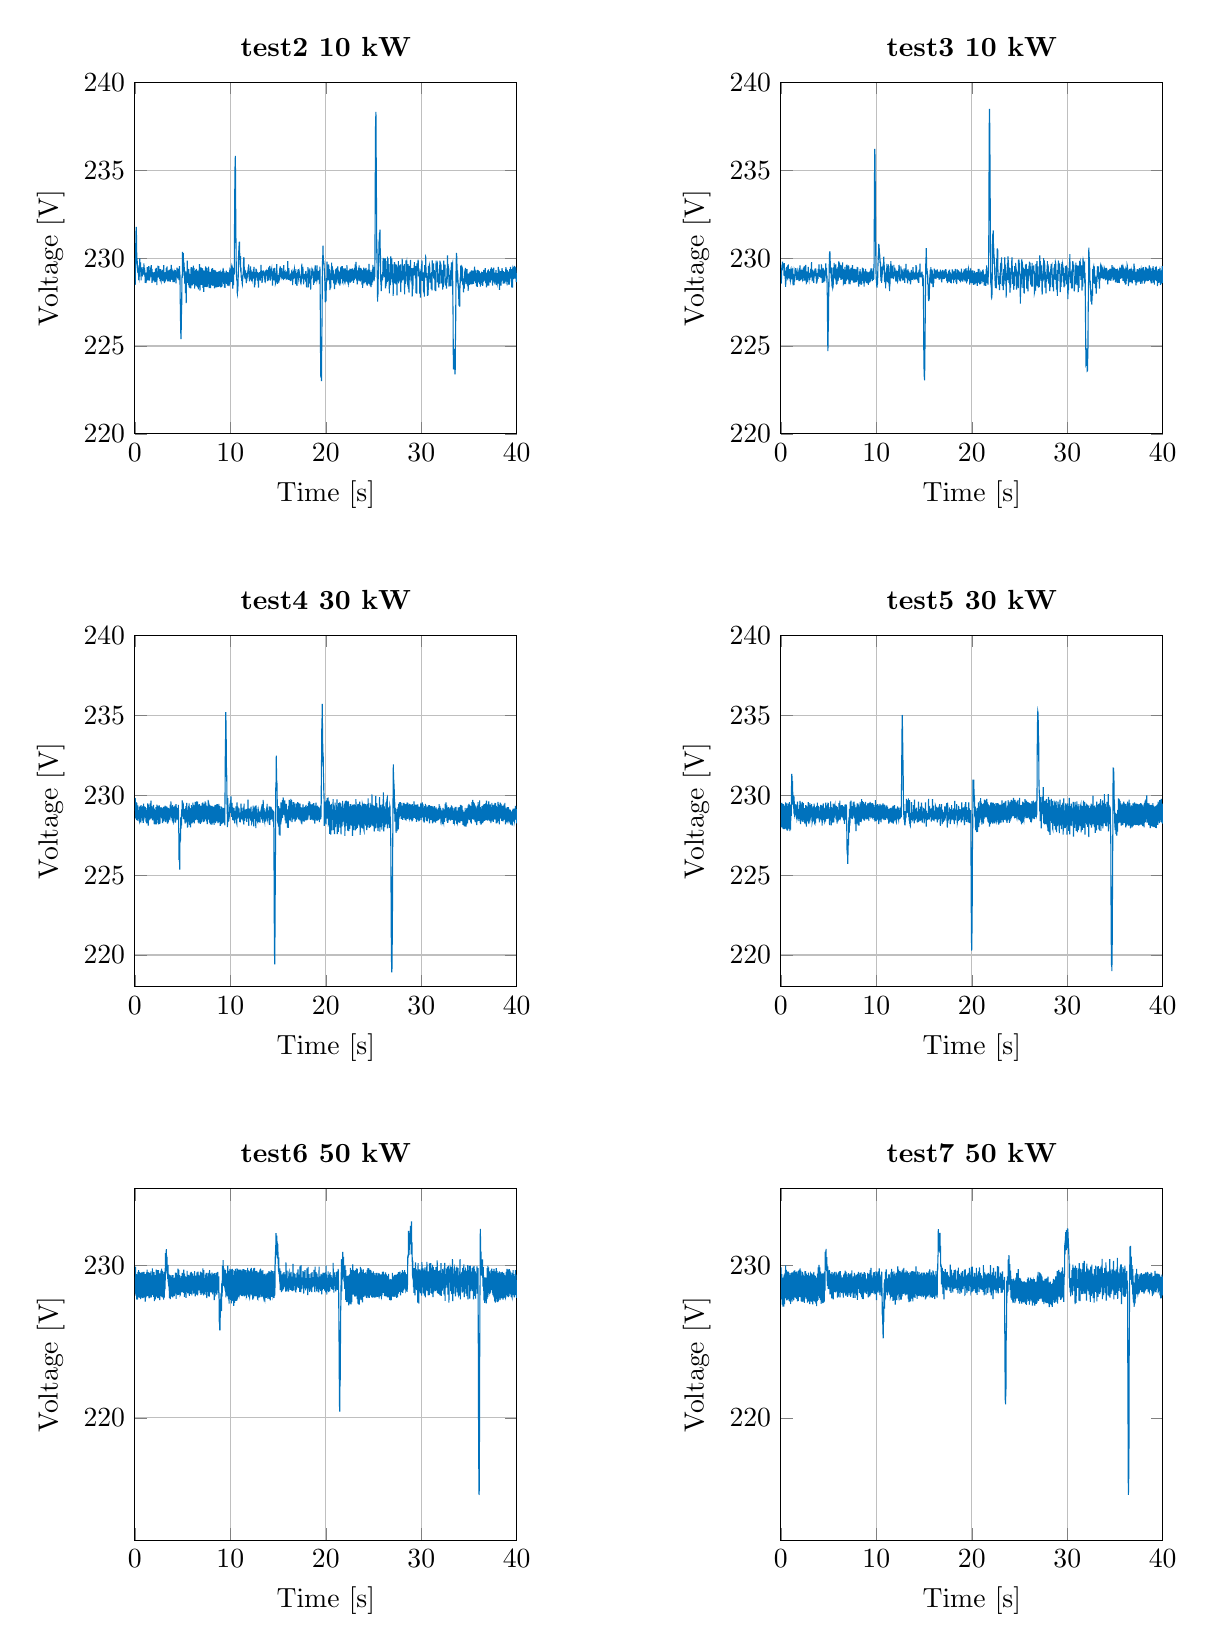
\begin{tikzpicture}

\begin{axis}[%
width=0.4\textwidth,
height=1.757in,
at={(0.953in,6.546in)},
scale only axis,
xmin=0,
xmax=40,
xmajorgrids,
xlabel={Time [s]},
ymin=220,
ymax=240,
ymajorgrids,
ylabel={Voltage [V]},
axis background/.style={fill=white},
title style={font=\bfseries},
title={test2 10 kW}
]
\addplot [color=mycolor1,solid,forget plot]
  table[row sep=crcr]{%
0.016	228.589250131759\\
0.032	228.488153960628\\
0.048	228.636377699998\\
0.064	229.777473408179\\
0.08	230.211188875522\\
0.096	230.789771927794\\
0.112	231.173527836619\\
0.128	231.641544209583\\
0.144	231.774688841467\\
0.16	231.560697132923\\
0.176	230.902758363097\\
0.192	230.325887683177\\
0.208	229.844795457389\\
0.224	229.692691612198\\
0.24	230.001759383036\\
0.256	229.426518899522\\
0.272	229.347056289144\\
0.288	229.387246527943\\
0.304	229.196656894186\\
0.32	229.460339683547\\
0.336	229.583177059539\\
0.352	229.445342767127\\
0.368	229.393524457909\\
0.384	229.085311723665\\
0.4	228.755910740743\\
0.416	229.19701150894\\
0.432	228.965094434767\\
0.448	228.902377265485\\
0.464	229.030072965443\\
0.48	229.304678578825\\
0.496	229.385942203911\\
0.512	229.992577472615\\
0.528	229.778164658484\\
0.544	229.637477926788\\
0.56	229.549512682031\\
0.576	229.418786740657\\
0.592	229.759867457206\\
0.608	229.208521746324\\
0.624	229.37616654287\\
0.64	229.206702283216\\
0.656	228.742028973797\\
0.672	229.472607947054\\
0.688	229.256747534275\\
0.704	229.103359990807\\
0.72	229.380623872988\\
0.736	228.979317334232\\
0.752	229.120603333575\\
0.768	229.384740924967\\
0.784	228.998690571028\\
0.8	229.178778101133\\
0.816	229.067699481222\\
0.832	229.093064722601\\
0.848	229.493406372089\\
0.864	229.379941429419\\
0.88	229.367330840133\\
0.896	229.295459131176\\
0.912	229.17037630167\\
0.928	229.152782148453\\
0.944	229.698317090679\\
0.96	229.330416229602\\
0.976	229.367616426882\\
0.992	229.138593724643\\
1.008	229.065304264191\\
1.024	229.44516167619\\
1.04	229.114293222866\\
1.056	229.073139115716\\
1.072	228.886883926452\\
1.088	228.595867968454\\
1.104	229.00566460575\\
1.12	229.17931165993\\
1.136	229.004677583295\\
1.152	229.028480845323\\
1.168	228.738115385695\\
1.184	228.576499152715\\
1.2	229.063400475903\\
1.216	228.902724541785\\
1.232	228.857764885983\\
1.248	228.740334956586\\
1.264	229.055766655582\\
1.28	229.16023291116\\
1.296	229.49107446454\\
1.312	229.280663659094\\
1.328	229.116421470804\\
1.344	229.024882555348\\
1.36	228.833603617074\\
1.376	229.179762105895\\
1.392	228.744810404902\\
1.408	228.928479340164\\
1.424	229.097747567405\\
1.44	228.912893134048\\
1.456	229.551324581169\\
1.472	229.362906024346\\
1.488	229.190902270921\\
1.504	229.312647221219\\
1.52	228.931650296096\\
1.536	228.719241206436\\
1.552	229.024779732203\\
1.568	228.855745627401\\
1.584	229.098335277699\\
1.6	228.915930817326\\
1.616	228.996704941522\\
1.632	229.294925943389\\
1.648	229.248081179349\\
1.664	229.426060671843\\
1.68	229.105356235649\\
1.696	228.96290768185\\
1.712	229.168802163832\\
1.728	229.601676583635\\
1.744	229.157669808932\\
1.76	229.193005864462\\
1.776	229.091057536764\\
1.792	228.590557408208\\
1.808	229.386501399228\\
1.824	228.962892224182\\
1.84	228.699670319012\\
1.856	228.831988934525\\
1.872	228.681514732993\\
1.888	229.001027722118\\
1.904	229.205608614045\\
1.92	229.145817677307\\
1.936	229.063205541511\\
1.952	228.876601699001\\
1.968	229.040370050678\\
1.984	229.168854005298\\
2	228.759223692416\\
2.016	229.017966595539\\
2.032	228.760769554549\\
2.048	228.741238215422\\
2.064	229.050026864175\\
2.08	229.203253233329\\
2.096	228.91243439817\\
2.112	229.227378025145\\
2.128	229.0406255899\\
2.144	228.639064719841\\
2.16	229.394025719431\\
2.176	229.046453082004\\
2.192	229.095035851975\\
2.208	229.19208879263\\
2.224	228.998694166476\\
2.24	229.441433136488\\
2.256	229.167391433026\\
2.272	229.252546628358\\
2.288	229.018715960883\\
2.304	228.473856772194\\
2.32	228.954763981423\\
2.336	229.144941996622\\
2.352	228.900092154562\\
2.368	229.235889443088\\
2.384	229.056705315616\\
2.4	228.911206764035\\
2.416	229.582899543171\\
2.432	229.251779740199\\
2.448	229.085973908733\\
2.464	228.978869850051\\
2.48	228.984246344999\\
2.496	229.096397661502\\
2.512	229.55199654854\\
2.528	229.317007022176\\
2.544	229.129884089141\\
2.56	228.899372367566\\
2.576	228.993319201294\\
2.592	229.32679410977\\
2.608	228.818022055958\\
2.624	229.033308668738\\
2.64	228.91180897083\\
2.656	228.693907129964\\
2.672	229.383593647725\\
2.688	229.14117578355\\
2.704	229.064386566238\\
2.72	229.122818514721\\
2.736	228.704081914584\\
2.752	228.677661978012\\
2.768	228.975317254056\\
2.784	228.752904720519\\
2.8	229.107236298924\\
2.816	229.09753841792\\
2.832	229.124808210525\\
2.848	229.346357931565\\
2.864	229.27711742133\\
2.88	229.280653670725\\
2.896	229.031628653769\\
2.912	228.697901329604\\
2.928	228.808532537421\\
2.944	229.259068749714\\
2.96	228.985282698253\\
2.976	229.284447614175\\
2.992	229.071547979065\\
3.008	228.732078090118\\
3.024	229.611828288045\\
3.04	229.081763480114\\
3.056	228.960287881124\\
3.072	228.864498397025\\
3.088	228.586083330343\\
3.104	228.963527915743\\
3.12	229.192733932058\\
3.136	228.996403869558\\
3.152	229.101144582656\\
3.168	228.727568340556\\
3.184	228.883480327821\\
3.2	229.201075869959\\
3.216	228.692077145071\\
3.232	229.046254928376\\
3.248	228.862211247222\\
3.264	228.901328739275\\
3.28	229.400004252667\\
3.296	229.412705747198\\
3.312	229.215010764067\\
3.328	229.372622663288\\
3.344	229.12850956785\\
3.36	229.082895238979\\
3.376	229.533301343549\\
3.392	228.986452233394\\
3.408	229.01603481445\\
3.424	229.006400198482\\
3.44	228.676359085164\\
3.456	229.288120584255\\
3.472	229.068495952071\\
3.488	229.052409850959\\
3.504	228.970988452981\\
3.52	228.685663866877\\
3.536	228.759336844231\\
3.552	229.250001687882\\
3.568	229.18463723112\\
3.584	229.332481734152\\
3.6	229.036761347737\\
3.616	229.07890856335\\
3.632	229.113716500209\\
3.648	229.062268335237\\
3.664	229.04965320399\\
3.68	228.76766637863\\
3.696	228.648968459691\\
3.712	228.761795055409\\
3.728	229.372689645384\\
3.744	229.211319234465\\
3.76	229.27108291328\\
3.776	229.207776657817\\
3.792	228.967394546197\\
3.808	229.622425058227\\
3.824	229.111902411441\\
3.84	229.01542853352\\
3.856	228.928707353881\\
3.872	228.767341611231\\
3.888	229.308168465434\\
3.904	229.234352791744\\
3.92	229.163750200489\\
3.936	229.1991059043\\
3.952	228.910780899835\\
3.968	229.050974962704\\
3.984	229.123015471032\\
4	228.645612811361\\
4.016	228.902145415263\\
4.032	228.778093437594\\
4.048	228.784109164199\\
4.064	229.214517146108\\
4.08	229.239691817385\\
4.096	229.026752175474\\
4.112	229.140935627012\\
4.128	228.960629179157\\
4.144	228.638741409377\\
4.16	229.307533570706\\
4.176	228.968324969391\\
4.192	228.97744666909\\
4.208	229.027466940534\\
4.224	228.902390637908\\
4.24	229.324904939113\\
4.256	229.003070867643\\
4.272	229.146754510802\\
4.288	228.882648708141\\
4.304	228.565915221549\\
4.32	228.868499558398\\
4.336	229.113915543947\\
4.352	228.909589758792\\
4.368	229.247889950412\\
4.384	229.064765325561\\
4.4	228.943887542789\\
4.416	229.464950957569\\
4.432	229.214956101785\\
4.448	228.941791400388\\
4.464	228.923015623069\\
4.48	228.992703135656\\
4.496	228.991813260614\\
4.512	229.4111068227\\
4.528	229.123939121929\\
4.544	228.976660386006\\
4.56	228.931306270532\\
4.576	228.84897732103\\
4.592	229.254113100425\\
4.608	228.759129666023\\
4.624	229.008067281965\\
4.64	229.170721548527\\
4.656	228.871636351592\\
4.672	229.547366903421\\
4.688	229.411607184542\\
4.704	229.069836172195\\
4.72	229.174972001997\\
4.736	228.37026250274\\
4.752	227.49245657523\\
4.768	227.276037573554\\
4.784	226.43778310086\\
4.8	226.316812896277\\
4.816	225.524525454755\\
4.832	225.388703724923\\
4.848	225.79486041467\\
4.864	226.156092356798\\
4.88	226.893394774652\\
4.896	226.80790884492\\
4.912	227.69259363137\\
4.928	228.877523205643\\
4.944	228.953361396038\\
4.96	229.033194297013\\
4.976	229.01489135641\\
4.992	230.358427442193\\
5.008	230.255614876532\\
5.024	229.853928185267\\
5.04	229.760954572301\\
5.056	229.608243812079\\
5.072	230.291031398291\\
5.088	229.949468922718\\
5.104	229.562635948531\\
5.12	229.379972667643\\
5.136	229.014314241804\\
5.152	229.747981547442\\
5.168	229.478092721048\\
5.184	229.441385901061\\
5.2	228.955700132768\\
5.216	228.556365761885\\
5.232	229.126514309185\\
5.248	229.282077389552\\
5.264	228.840812071346\\
5.28	228.892667131018\\
5.296	228.015727317039\\
5.312	228.343758925541\\
5.328	228.52170539948\\
5.344	228.088186336221\\
5.36	228.184088493372\\
5.376	227.446051777275\\
5.392	228.119031171397\\
5.408	228.908520306546\\
5.424	228.86699865079\\
5.44	229.16230455724\\
5.456	228.64517840704\\
5.472	229.565727829464\\
5.488	229.85600287239\\
5.504	229.524442404001\\
5.52	229.290989801437\\
5.536	228.60095316342\\
5.552	229.177732235854\\
5.568	229.327711227545\\
5.584	228.929819280482\\
5.6	229.021066693152\\
5.616	228.471668709931\\
5.632	229.133924325356\\
5.648	229.383056059527\\
5.664	229.056817204841\\
5.68	229.164498158135\\
5.696	228.344917762558\\
5.712	228.724840654901\\
5.728	229.062005681671\\
5.744	228.789404293821\\
5.76	229.098807402154\\
5.776	228.294673463027\\
5.792	228.766012944352\\
5.808	229.075352864679\\
5.824	228.707889870648\\
5.84	228.962039522008\\
5.856	228.276629891502\\
5.872	228.864495717332\\
5.888	229.488618868586\\
5.904	229.289842216676\\
5.92	229.493652391169\\
5.936	228.791551639125\\
5.952	229.292592933588\\
5.968	229.472630618599\\
5.984	229.00762405036\\
6	229.080200930214\\
6.016	228.455647821348\\
6.032	229.003362329668\\
6.048	229.415170590573\\
6.064	229.092501101094\\
6.08	229.24196127715\\
6.096	228.535099516838\\
6.112	229.171099547055\\
6.128	229.571805661705\\
6.144	229.211814014897\\
6.16	229.29944390887\\
6.176	228.518886938169\\
6.192	228.98052462192\\
6.208	229.44148102427\\
6.224	228.964604369308\\
6.24	229.023677645726\\
6.256	228.273891712585\\
6.272	228.771565681894\\
6.288	229.26596825231\\
6.304	229.050828139325\\
6.32	229.182427368437\\
6.336	228.48407520532\\
6.352	228.912595348409\\
6.368	229.331861207744\\
6.384	229.026973745296\\
6.4	229.189487489786\\
6.416	228.396426036275\\
6.432	228.976731979422\\
6.448	229.388252790918\\
6.464	229.087602224015\\
6.48	229.198139445702\\
6.496	228.434018658389\\
6.512	228.845386047052\\
6.528	229.289147540814\\
6.544	228.927152580117\\
6.56	229.098750647588\\
6.576	228.335456639105\\
6.592	228.814438948124\\
6.608	229.12235681591\\
6.624	228.80684456332\\
6.64	228.926794351765\\
6.656	228.224569136484\\
6.672	228.699217080634\\
6.688	229.253806876763\\
6.704	229.071580008867\\
6.72	229.334276185343\\
6.736	228.686036115033\\
6.752	229.351409124626\\
6.768	229.66143742288\\
6.784	229.08629307896\\
6.8	228.961010109575\\
6.816	228.151251813078\\
6.832	228.71789589398\\
6.848	229.190544449233\\
6.864	228.996360975867\\
6.88	229.249582152663\\
6.896	228.524513389581\\
6.912	229.130884547265\\
6.928	229.472508587893\\
6.944	229.141042052759\\
6.96	229.194854602202\\
6.976	228.479687895542\\
6.992	229.017272595344\\
7.008	229.436032454547\\
7.024	229.137098819335\\
7.04	229.215932305443\\
7.056	228.475077633686\\
7.072	229.116548327598\\
7.088	229.418428581475\\
7.104	228.966035762493\\
7.12	228.941847367964\\
7.136	228.307777556668\\
7.152	228.908932989033\\
7.168	229.301998865268\\
7.184	228.84470432451\\
7.2	228.883016188506\\
7.216	228.08618352875\\
7.232	228.67089119179\\
7.248	229.072195626812\\
7.264	228.812421700539\\
7.28	228.995462076572\\
7.296	228.42484063252\\
7.312	228.928845679737\\
7.328	229.309864126039\\
7.344	228.946937015959\\
7.36	229.021178617857\\
7.376	228.36649616413\\
7.392	229.173830361276\\
7.408	229.527303855532\\
7.424	229.195232036175\\
7.44	229.186630877699\\
7.456	228.550195459539\\
7.472	229.186484870131\\
7.488	229.459232296943\\
7.504	229.01572859176\\
7.52	229.039035709815\\
7.536	228.346852787933\\
7.552	228.999167983938\\
7.568	229.27605071433\\
7.584	228.992929313249\\
7.6	228.985186280622\\
7.616	228.380429930941\\
7.632	229.110882096537\\
7.648	229.447059498288\\
7.664	229.140218131379\\
7.68	229.151891923503\\
7.696	228.544885551709\\
7.712	229.264958969237\\
7.728	229.520261256804\\
7.744	229.166119715727\\
7.76	229.024491718677\\
7.776	228.301235319839\\
7.792	228.924023075007\\
7.808	229.178802638719\\
7.824	228.874159196609\\
7.84	228.944778209981\\
7.856	228.30758857617\\
7.872	229.011227520977\\
7.888	229.219959543331\\
7.904	228.93108189392\\
7.92	228.907172669531\\
7.936	228.296934675473\\
7.952	228.97911071584\\
7.968	229.206159046098\\
7.984	228.980602355053\\
8	229.120946107982\\
8.016	228.488098985402\\
8.032	229.244865669389\\
8.048	229.396589423104\\
8.064	229.118070402521\\
8.08	229.004448064822\\
8.096	228.448173986382\\
8.112	229.197897085077\\
8.128	229.440629863824\\
8.144	229.180299542593\\
8.16	229.053525425523\\
8.176	228.430514892561\\
8.192	229.106768769192\\
8.208	229.272523422365\\
8.224	229.074990366949\\
8.24	229.018066832895\\
8.256	228.450870041751\\
8.272	229.124142098411\\
8.288	229.329797682674\\
8.304	229.016041325312\\
8.32	228.956429512381\\
8.336	228.280989873902\\
8.352	229.048054167797\\
8.368	229.23553239643\\
8.384	228.969019280884\\
8.4	228.927737264006\\
8.416	228.396618953195\\
8.432	229.082553240251\\
8.448	229.300422495184\\
8.464	228.976032416728\\
8.48	228.94759140186\\
8.496	228.343454154661\\
8.512	229.085010466036\\
8.528	229.199749695471\\
8.544	228.926861434377\\
8.56	228.852432478191\\
8.576	228.341527825507\\
8.592	229.015353109485\\
8.608	229.219930522763\\
8.624	229.004171360989\\
8.64	228.909111070338\\
8.656	228.36605274089\\
8.672	229.130658038421\\
8.688	229.205007994044\\
8.704	228.956739508897\\
8.72	228.740129049352\\
8.736	228.364282987619\\
8.752	229.027785267973\\
8.768	229.24771770128\\
8.784	229.001917728641\\
8.8	228.8100273341\\
8.816	228.394938505452\\
8.832	229.07231878284\\
8.848	229.109672162347\\
8.864	229.043209423319\\
8.88	228.922310361074\\
8.896	228.525062669797\\
8.912	229.156533396398\\
8.928	229.182027109359\\
8.944	228.956830439632\\
8.96	228.772463698963\\
8.976	228.341891168712\\
8.992	229.023210801865\\
9.008	229.060828033045\\
9.024	228.911851514227\\
9.04	228.664124844383\\
9.056	228.354005353736\\
9.072	229.091311984316\\
9.088	229.218065861687\\
9.104	228.963572508684\\
9.12	228.775967559402\\
9.136	228.393534252914\\
9.152	229.101624733394\\
9.168	229.145771634347\\
9.184	229.109928090886\\
9.2	229.003939980928\\
9.216	228.619821550617\\
9.232	229.325451596742\\
9.248	229.450543403886\\
9.264	229.190037020513\\
9.28	229.017339583731\\
9.296	228.545848817964\\
9.312	229.256081167075\\
9.328	229.19157816764\\
9.344	228.944153841106\\
9.36	228.72839129685\\
9.376	228.327066879465\\
9.392	228.987160622198\\
9.408	229.089538124977\\
9.424	228.868673578846\\
9.44	228.684758011978\\
9.456	228.315028136164\\
9.472	229.072064316539\\
9.488	229.052838480562\\
9.504	228.971848891243\\
9.52	228.81192082529\\
9.536	228.571277373418\\
9.552	229.183675617618\\
9.568	229.293769166896\\
9.584	229.168142960656\\
9.6	228.925814890451\\
9.616	228.536143154109\\
9.632	229.160369314608\\
9.648	229.157452016749\\
9.664	229.013981318278\\
9.68	228.757396603449\\
9.696	228.441946125321\\
9.712	229.111663593345\\
9.728	229.20655921228\\
9.744	229.051885283678\\
9.76	228.834541350192\\
9.776	228.45277259135\\
9.792	229.131364685593\\
9.808	229.123766194526\\
9.824	228.958038020792\\
9.84	228.666344637077\\
9.856	228.407171513218\\
9.872	229.082896566191\\
9.888	229.136198013215\\
9.904	229.027258434218\\
9.92	228.776480698595\\
9.936	228.503335654403\\
9.952	229.276057490143\\
9.968	229.243988647358\\
9.984	229.198577836607\\
10	228.863934516823\\
10.016	228.67799528788\\
10.032	229.389053771172\\
10.048	229.393429316601\\
10.064	229.193945555901\\
10.08	228.910290430209\\
10.096	228.645836193406\\
10.112	229.419685182103\\
10.128	229.386250631403\\
10.144	229.341273144598\\
10.16	229.021629960494\\
10.176	228.80803562235\\
10.192	229.50706397471\\
10.208	229.473298413388\\
10.224	229.165384209675\\
10.24	228.713270761956\\
10.256	228.272312274068\\
10.272	228.942728830751\\
10.288	228.894129107413\\
10.304	228.872830964291\\
10.32	228.549930639109\\
10.336	228.465350818854\\
10.352	229.368566737001\\
10.368	229.454164359313\\
10.384	229.302737337525\\
10.4	229.0678091376\\
10.416	229.182031270574\\
10.432	231.006053868391\\
10.448	232.500641888805\\
10.464	233.66360087204\\
10.48	234.74398235112\\
10.496	235.26334421739\\
10.512	235.623089595535\\
10.528	235.818955324497\\
10.544	234.322128361949\\
10.56	232.90880471716\\
10.576	231.9870021155\\
10.592	230.840329132639\\
10.608	230.180072110931\\
10.624	229.193651116446\\
10.64	229.06299498465\\
10.656	228.890267182431\\
10.672	228.762161993756\\
10.688	228.727592092729\\
10.704	228.794872827379\\
10.72	228.040277301766\\
10.736	227.995211166728\\
10.752	228.41193452108\\
10.768	228.212847587195\\
10.784	228.118514079125\\
10.8	228.450046615152\\
10.816	228.745799400462\\
10.832	229.09836156779\\
10.848	229.867857870233\\
10.864	230.180041515734\\
10.88	230.246814504266\\
10.896	230.664803508983\\
10.912	230.663512808806\\
10.928	230.917111475757\\
10.944	230.703703775119\\
10.96	230.943029594337\\
10.976	230.285405569304\\
10.992	230.275604348997\\
11.008	229.910161187194\\
11.024	229.473314955856\\
11.04	229.714095125695\\
11.056	229.558854387538\\
11.072	230.113270006063\\
11.088	229.345483420184\\
11.104	229.181884903499\\
11.12	229.461556824683\\
11.136	229.008701799602\\
11.152	228.88995570655\\
11.168	228.888739159583\\
11.184	228.991438107568\\
11.2	228.708251967992\\
11.216	229.024307497902\\
11.232	228.835412255285\\
11.248	228.544820209378\\
11.264	228.508559111696\\
11.28	229.015908805793\\
11.296	228.844587843041\\
11.312	228.843456497225\\
11.328	229.061511405477\\
11.344	229.130845269734\\
11.36	229.249653146726\\
11.376	229.54906334073\\
11.392	230.011431121031\\
11.408	229.844633407677\\
11.424	230.063106574095\\
11.44	229.579664556775\\
11.456	229.48600640939\\
11.472	229.030142601574\\
11.488	229.37965759277\\
11.504	229.025863310723\\
11.52	228.865941693963\\
11.536	229.027144370146\\
11.552	228.808183902834\\
11.568	229.016150482247\\
11.584	229.05943568886\\
11.6	229.312063113705\\
11.616	228.869768023059\\
11.632	229.049575383012\\
11.648	229.146617350673\\
11.664	228.627932809439\\
11.68	228.622593620936\\
11.696	228.85159580085\\
11.712	229.056754207727\\
11.728	228.693506234791\\
11.744	228.885004799304\\
11.76	229.169412946728\\
11.776	228.92632797096\\
11.792	228.935735430705\\
11.808	229.239462474395\\
11.824	229.170080843157\\
11.84	229.252408858499\\
11.856	229.187530088373\\
11.872	229.182800814811\\
11.888	229.168583576339\\
11.904	229.431039453843\\
11.92	229.647301100445\\
11.936	229.309035396902\\
11.952	229.425763658519\\
11.968	228.86887047613\\
11.984	228.867269955341\\
12	228.675048380232\\
12.016	229.26839470382\\
12.032	228.898930736759\\
12.048	228.773549383854\\
12.064	229.154857198147\\
12.08	228.850850386741\\
12.096	228.978271193713\\
12.112	228.822915800653\\
12.128	229.538582012944\\
12.144	228.809976050213\\
12.16	228.911809574668\\
12.176	228.941373193322\\
12.192	228.903643350174\\
12.208	228.676688148139\\
12.224	228.880245063457\\
12.24	229.067733161913\\
12.256	229.018848252686\\
12.272	228.935679673271\\
12.288	228.890092011364\\
12.304	228.82757887832\\
12.32	228.938415965467\\
12.336	229.23688421914\\
12.352	228.9412522186\\
12.368	229.169757008596\\
12.384	229.029488681484\\
12.4	229.001214165316\\
12.416	228.842945492658\\
12.432	229.373851234486\\
12.448	229.309092889218\\
12.464	229.268429245987\\
12.48	229.503818828428\\
12.496	229.31870630099\\
12.512	228.81708754664\\
12.528	228.333015635405\\
12.544	229.206957896275\\
12.56	228.621379753159\\
12.576	228.469922723854\\
12.592	228.658045240991\\
12.608	228.743418631371\\
12.624	228.757692132548\\
12.64	228.767873691838\\
12.656	229.169289946535\\
12.672	229.072953853618\\
12.688	229.359208798903\\
12.704	229.356812492586\\
12.72	229.195514636498\\
12.736	229.327109529586\\
12.752	229.315530260062\\
12.768	229.18553153981\\
12.784	228.908988985979\\
12.8	229.178497646801\\
12.816	229.028453666438\\
12.832	228.730427822081\\
12.848	229.044302541352\\
12.864	229.211256348261\\
12.88	228.731313119006\\
12.896	228.726905135348\\
12.912	228.970278068093\\
12.928	228.580592666966\\
12.944	228.329668360342\\
12.96	228.769865012726\\
12.976	229.098630892453\\
12.992	228.98026903347\\
13.008	229.118269915946\\
13.024	229.029799003072\\
13.04	229.210151055137\\
13.056	228.777716912907\\
13.072	229.132252461576\\
13.088	228.808067493371\\
13.104	229.021475700145\\
13.12	228.913447028742\\
13.136	228.73036226225\\
13.152	228.952493423919\\
13.168	228.979242652276\\
13.184	229.262180146543\\
13.2	229.059545307797\\
13.216	229.620353449314\\
13.232	229.282521257082\\
13.248	228.965495605473\\
13.264	228.940581999252\\
13.28	229.315808305942\\
13.296	228.927114993236\\
13.312	228.600006849918\\
13.328	228.727776029688\\
13.344	228.759850749909\\
13.36	228.66405093603\\
13.376	228.966892432767\\
13.392	229.279154229368\\
13.408	229.097158925039\\
13.424	229.208574099294\\
13.44	229.215804582249\\
13.456	229.195455240583\\
13.472	229.127459153668\\
13.488	229.306831036827\\
13.504	229.041114791443\\
13.52	229.030213651031\\
13.536	229.136950078907\\
13.552	228.979855358873\\
13.568	229.091178491182\\
13.584	228.87465210718\\
13.6	229.107339611934\\
13.616	228.621749901062\\
13.632	228.887841907301\\
13.648	229.248363116063\\
13.664	228.900957825203\\
13.68	228.842665178374\\
13.696	228.990726986394\\
13.712	229.306506129166\\
13.728	229.020450976912\\
13.744	229.149928168544\\
13.76	229.155574006375\\
13.776	229.189341902095\\
13.792	229.010189742642\\
13.808	229.329865581423\\
13.824	229.208787399251\\
13.84	229.295510365671\\
13.856	228.965555788569\\
13.872	229.056372791099\\
13.888	228.702407734928\\
13.904	229.016880249468\\
13.92	229.172093732916\\
13.936	228.971441984954\\
13.952	229.345995994008\\
13.968	229.056999737598\\
13.984	228.945666769378\\
14	228.739874205061\\
14.016	229.480513992719\\
14.032	229.012741843958\\
14.048	229.014842880354\\
14.064	229.211280098623\\
14.08	229.066825995181\\
14.096	229.002095723073\\
14.112	228.908941046861\\
14.128	229.559185048656\\
14.144	229.024656552742\\
14.16	228.903261598678\\
14.176	228.896017323098\\
14.192	228.730786792496\\
14.208	228.809218180479\\
14.224	228.961594331484\\
14.24	229.11774972581\\
14.256	229.129210493961\\
14.272	229.242044489256\\
14.288	229.203833987247\\
14.304	229.064773573988\\
14.32	229.323193578553\\
14.336	229.374237874997\\
14.352	229.140484852722\\
14.368	229.167841096195\\
14.384	229.272570811833\\
14.4	228.67988567025\\
14.416	228.441421113902\\
14.432	228.884058575859\\
14.448	229.01781422671\\
14.464	228.73252623473\\
14.48	228.954395675327\\
14.496	229.084549388544\\
14.512	229.203254203189\\
14.528	228.914047972685\\
14.544	229.423903797884\\
14.56	229.201039426771\\
14.576	229.159717872447\\
14.592	229.021936090445\\
14.608	228.737840055347\\
14.624	229.025936063145\\
14.64	228.850808405258\\
14.656	229.445133877842\\
14.672	228.978132497774\\
14.688	229.154605655079\\
14.704	228.741357780631\\
14.72	228.543006239136\\
14.736	228.572389933145\\
14.752	228.862768784926\\
14.768	228.609464810518\\
14.784	228.662920919542\\
14.8	229.093204538478\\
14.816	229.15590862428\\
14.832	229.027148879001\\
14.848	229.183613212204\\
14.864	229.658307245627\\
14.88	229.30490563733\\
14.896	229.194733196702\\
14.912	228.838617434022\\
14.928	228.887876067099\\
14.944	228.543050533179\\
14.96	229.046379029196\\
14.976	228.894712469415\\
14.992	229.001467105987\\
15.008	228.928408005443\\
15.024	228.862251503166\\
15.04	228.867415813577\\
15.056	228.713184633128\\
15.072	228.929326179837\\
15.088	228.615781031557\\
15.104	229.059516697653\\
15.12	229.139964413432\\
15.136	228.77881366056\\
15.152	228.801047508691\\
15.168	229.139817780355\\
15.184	229.448469893164\\
15.2	229.243876543389\\
15.216	229.341958959817\\
15.232	229.536435659353\\
15.248	229.033358450923\\
15.264	228.930912446965\\
15.28	229.197094979277\\
15.296	229.254770236535\\
15.312	229.038360988547\\
15.328	229.136865224087\\
15.344	229.005693099762\\
15.36	229.057335946171\\
15.376	229.160995809427\\
15.392	229.452932084788\\
15.408	229.271130688016\\
15.424	229.285885358638\\
15.44	228.938714891364\\
15.456	228.948088670457\\
15.472	228.831846690353\\
15.488	229.243132924171\\
15.504	229.06983556056\\
15.52	228.86543823554\\
15.536	229.155862722218\\
15.552	228.751579032693\\
15.568	228.875185471225\\
15.584	228.871133567735\\
15.6	229.599731644225\\
15.616	228.90936114183\\
15.632	228.991195013589\\
15.648	229.102094324404\\
15.664	229.007243338054\\
15.68	228.812081701598\\
15.696	229.018385894613\\
15.712	229.259339728228\\
15.728	229.190216018542\\
15.744	229.218888972376\\
15.76	229.151317270478\\
15.776	229.101202294967\\
15.792	228.958888105595\\
15.808	229.205786504188\\
15.824	228.845290362385\\
15.84	229.103973290688\\
15.856	228.927318924479\\
15.872	228.959962875628\\
15.888	228.784330906626\\
15.904	229.235701707531\\
15.92	229.093487064726\\
15.936	228.975254695289\\
15.952	229.264326428605\\
15.968	229.109018304684\\
15.984	228.965275642896\\
16	228.803413668966\\
16.016	229.828841461106\\
16.032	229.447785327217\\
16.048	229.216583548873\\
16.064	229.038254222665\\
16.08	228.772521708928\\
16.096	228.857085146506\\
16.112	229.056507909054\\
16.128	229.438604186293\\
16.144	229.222166526784\\
16.16	229.052376941372\\
16.176	228.999636644168\\
16.192	228.881795338188\\
16.208	228.824341877022\\
16.224	228.756219027082\\
16.24	228.956956600263\\
16.256	228.973354056719\\
16.272	229.020779945435\\
16.288	229.040574753482\\
16.304	228.697646940459\\
16.32	228.866548495942\\
16.336	229.019475793629\\
16.352	228.697647710613\\
16.368	228.747921655149\\
16.384	229.126981147792\\
16.4	229.020086404851\\
16.416	228.86171634984\\
16.432	229.282083773296\\
16.448	229.296557277741\\
16.464	228.839575402512\\
16.48	228.911270271088\\
16.496	228.882838211206\\
16.512	228.929783881722\\
16.528	228.461008353852\\
16.544	229.150742040684\\
16.56	228.962452110283\\
16.576	229.228960751235\\
16.592	229.03806952261\\
16.608	228.811332125661\\
16.624	228.879609537463\\
16.64	229.18366352649\\
16.656	229.339367634781\\
16.672	229.02986167065\\
16.688	229.31742501265\\
16.704	229.363849119221\\
16.72	229.060697030932\\
16.736	228.970949777851\\
16.752	229.264941853459\\
16.768	228.943398290298\\
16.784	228.842801731415\\
16.8	229.109394471649\\
16.816	228.996274009821\\
16.832	228.527844756291\\
16.848	228.83919852344\\
16.864	229.373657794691\\
16.88	228.951684845782\\
16.896	228.911862679188\\
16.912	228.728633055027\\
16.928	228.795758516978\\
16.944	228.485403419917\\
16.96	228.704605191698\\
16.976	228.426130761726\\
16.992	228.661570711831\\
17.008	228.925042701398\\
17.024	229.049246698009\\
17.04	229.155260856061\\
17.056	228.947074699889\\
17.072	229.32605704854\\
17.088	228.917221313947\\
17.104	229.136258163201\\
17.12	229.378795579387\\
17.136	228.890174776105\\
17.152	228.829927100734\\
17.168	228.959355315104\\
17.184	229.212712167188\\
17.2	228.880824004391\\
17.216	229.015899538939\\
17.232	229.101488714744\\
17.248	229.151105548553\\
17.264	228.89792201849\\
17.28	229.083865021319\\
17.296	229.063430474334\\
17.312	229.023941230988\\
17.328	228.942727190893\\
17.344	228.785919140637\\
17.36	228.621138646531\\
17.376	228.595386154839\\
17.392	228.77511814514\\
17.408	228.509539082908\\
17.424	228.868884009888\\
17.44	228.66526984348\\
17.456	228.917571949627\\
17.472	228.999960681607\\
17.488	229.695534719659\\
17.504	229.161878372204\\
17.52	229.141365587755\\
17.536	229.248268225368\\
17.552	229.142593678412\\
17.568	228.990560694014\\
17.584	228.832038796674\\
17.6	229.512236847846\\
17.616	229.180644015238\\
17.632	229.077536882773\\
17.648	229.016109159053\\
17.664	228.667004391996\\
17.68	228.510142345525\\
17.696	228.850307984432\\
17.712	228.961602603242\\
17.728	228.978646931372\\
17.744	228.948727761827\\
17.76	229.102926793504\\
17.776	228.978245017227\\
17.792	229.097581128864\\
17.808	229.01303763265\\
17.824	228.830185893993\\
17.84	228.949954861903\\
17.856	229.126999477531\\
17.872	228.904125756887\\
17.888	228.661219445556\\
17.904	229.235649956966\\
17.92	229.239985437463\\
17.936	228.800296963201\\
17.952	228.73169985146\\
17.968	228.722258149845\\
17.984	228.374125577017\\
18	228.370075133524\\
18.016	229.084544929449\\
18.032	229.023928331909\\
18.048	228.883899079548\\
18.064	229.082605421707\\
18.08	228.870674379476\\
18.096	229.127928709984\\
18.112	228.917755771235\\
18.128	229.485230485291\\
18.144	229.07429718808\\
18.16	229.275683779567\\
18.176	228.828994812503\\
18.192	228.345022766035\\
18.208	228.542957533453\\
18.224	228.95070059714\\
18.24	228.868728722269\\
18.256	228.976140831368\\
18.272	229.354517098819\\
18.288	229.133485322144\\
18.304	229.198038439712\\
18.32	229.292553878455\\
18.336	229.417317868367\\
18.352	228.676278278891\\
18.368	228.692716647816\\
18.384	228.640814587057\\
18.4	228.664695859514\\
18.416	228.21786405217\\
18.432	228.77527050467\\
18.448	228.881990714606\\
18.464	228.992470768148\\
18.48	228.871988055649\\
18.496	228.863884941038\\
18.512	229.069811134878\\
18.528	229.18505640516\\
18.544	229.430432807472\\
18.56	229.101845920536\\
18.576	229.371744826439\\
18.592	229.350975083124\\
18.608	229.135261342117\\
18.624	229.089994501818\\
18.64	229.009302485933\\
18.656	229.158973523189\\
18.672	228.881779977083\\
18.688	229.072339715427\\
18.704	229.112189150931\\
18.72	228.48833862486\\
18.736	228.599077658011\\
18.752	229.252434443331\\
18.768	229.02511955618\\
18.784	228.604920670429\\
18.8	228.691580983564\\
18.816	228.867234636286\\
18.832	229.111663371626\\
18.848	229.174824741852\\
18.864	229.455023048012\\
18.88	229.357701690863\\
18.896	229.591529017636\\
18.912	229.246465571629\\
18.928	229.082246196304\\
18.944	228.675929518298\\
18.96	229.306859849393\\
18.976	229.133172545627\\
18.992	229.029335537327\\
19.008	229.360061269767\\
19.024	228.888107642659\\
19.04	228.990838763878\\
19.056	229.008418070027\\
19.072	229.592704595413\\
19.088	228.78343299603\\
19.104	228.825377546441\\
19.12	229.069995591514\\
19.136	228.992897208734\\
19.152	228.781920835862\\
19.168	228.86022170702\\
19.184	229.178258866166\\
19.2	229.083381980906\\
19.216	229.281494806862\\
19.232	229.203175872585\\
19.248	228.986718419312\\
19.264	228.96795474909\\
19.28	229.277303460687\\
19.296	228.777047043625\\
19.312	228.824902724474\\
19.328	228.660315196545\\
19.344	228.682376056217\\
19.36	228.847600506538\\
19.376	229.515842875897\\
19.392	229.322694012505\\
19.408	228.28282697972\\
19.424	227.033510112372\\
19.44	225.39141959215\\
19.456	224.129603610966\\
19.472	223.271865453401\\
19.488	223.3974003916\\
19.504	223.190901312394\\
19.52	223.507910286332\\
19.536	223.396959516016\\
19.552	223.002449943422\\
19.568	224.624013933912\\
19.584	225.628040953343\\
19.6	226.277215863099\\
19.616	226.950799804595\\
19.632	228.911351964508\\
19.648	229.794779173399\\
19.664	229.873490265333\\
19.68	230.083522666716\\
19.696	230.32391629329\\
19.712	230.711705073381\\
19.728	230.10137140497\\
19.744	229.85595762485\\
19.76	229.759808189299\\
19.776	229.774491756986\\
19.792	229.854226596412\\
19.808	229.694127627849\\
19.824	229.505571682455\\
19.84	229.316002121987\\
19.856	229.21194639446\\
19.872	229.023121696468\\
19.888	228.992635848793\\
19.904	228.385531675063\\
19.92	228.163353932722\\
19.936	227.604968371321\\
19.952	227.48098686264\\
19.968	228.108239356845\\
19.984	227.910607783353\\
20	227.866468486529\\
20.016	227.544837864994\\
20.032	227.619654043246\\
20.048	228.601156614746\\
20.064	228.727089050572\\
20.08	228.865913191425\\
20.096	228.632648648621\\
20.112	229.064200400603\\
20.128	229.801076402084\\
20.144	229.497076149807\\
20.16	229.338484525169\\
20.176	228.96519198043\\
20.192	229.298055447649\\
20.208	229.627666839896\\
20.224	229.315435173645\\
20.24	229.25612159573\\
20.256	228.740371918316\\
20.272	228.876107956826\\
20.288	229.647216818292\\
20.304	229.47819461869\\
20.32	229.581592354767\\
20.336	229.129572786119\\
20.352	229.021448023888\\
20.368	229.379455937708\\
20.384	229.082548482714\\
20.4	228.861629552397\\
20.416	228.59657711908\\
20.432	228.182895083364\\
20.448	228.751740304725\\
20.464	228.552815018776\\
20.48	228.566322478665\\
20.496	228.332474155544\\
20.512	228.331942561831\\
20.528	229.17540079671\\
20.544	229.153196486854\\
20.56	229.240680181899\\
20.576	229.021555409972\\
20.592	229.088148532743\\
20.608	229.752497783517\\
20.624	229.400164322429\\
20.64	229.255836815772\\
20.656	228.764091951256\\
20.672	228.975864136386\\
20.688	229.52719775544\\
20.704	229.358878027717\\
20.72	229.286447355119\\
20.736	228.880676467771\\
20.752	228.742494670342\\
20.768	229.284790339239\\
20.784	229.147899670504\\
20.8	229.17432930172\\
20.816	228.880988506185\\
20.832	228.571483271231\\
20.848	229.107039879183\\
20.864	229.006596088693\\
20.88	228.904067377106\\
20.896	228.636856236311\\
20.912	228.240704566829\\
20.928	229.035278612299\\
20.944	228.98382091511\\
20.96	228.989095579741\\
20.976	228.667284895344\\
20.992	228.496595282137\\
21.008	229.332598206903\\
21.024	229.336743710119\\
21.04	229.129870433796\\
21.056	228.87222625378\\
21.072	228.703325287166\\
21.088	229.408572527318\\
21.104	229.187375021012\\
21.12	229.130426330906\\
21.136	228.785585013223\\
21.152	228.833524206954\\
21.168	229.448817008946\\
21.184	229.320208150576\\
21.2	229.297069564458\\
21.216	228.98769479783\\
21.232	228.906085673189\\
21.248	229.531998036582\\
21.264	229.378610584631\\
21.28	229.282446313235\\
21.296	228.798775144934\\
21.312	228.577621198351\\
21.328	229.294366101446\\
21.344	229.168361324668\\
21.36	229.015793403222\\
21.376	228.826474218212\\
21.392	228.517750826094\\
21.408	229.230377034977\\
21.424	229.021097374974\\
21.44	228.897913906755\\
21.456	228.615786089319\\
21.472	228.445387698411\\
21.488	229.112263250694\\
21.504	229.017320073312\\
21.52	228.953364770684\\
21.536	228.760275940068\\
21.552	228.728414162801\\
21.568	229.480742231991\\
21.584	229.332388977537\\
21.6	229.246839581741\\
21.616	228.867773030595\\
21.632	228.861713669352\\
21.648	229.529415737632\\
21.664	229.358628040651\\
21.68	229.253482926328\\
21.696	228.987782097704\\
21.712	228.865972425066\\
21.728	229.544387398165\\
21.744	229.200195094359\\
21.76	228.980564172781\\
21.776	228.61370021761\\
21.792	228.592625292959\\
21.808	229.238818908912\\
21.824	229.210192939852\\
21.84	229.084008828454\\
21.856	228.905847129287\\
21.872	228.790125725779\\
21.888	229.439142367704\\
21.904	229.202545117705\\
21.92	229.103840700473\\
21.936	228.713507506439\\
21.952	228.686546058531\\
21.968	229.370596387771\\
21.984	229.234759693284\\
22	229.114582179461\\
22.016	228.77405041939\\
22.032	228.734260947269\\
22.048	229.422380799017\\
22.064	229.109832174681\\
22.08	229.07020344262\\
22.096	228.673866857524\\
22.112	228.722727614976\\
22.128	229.314512641823\\
22.144	229.107440596027\\
22.16	229.034839278638\\
22.176	228.672183320893\\
22.192	228.76530280146\\
22.208	229.602810581709\\
22.224	229.403764762667\\
22.24	229.285782806907\\
22.256	228.737840873105\\
22.272	228.705868054264\\
22.288	229.28937356394\\
22.304	229.071909678372\\
22.32	229.010329405425\\
22.336	228.660751260215\\
22.352	228.623566872384\\
22.368	229.289852040321\\
22.384	228.978686274034\\
22.4	228.940324769208\\
22.416	228.639138861931\\
22.432	228.687139790722\\
22.448	229.316164604711\\
22.464	229.140907410926\\
22.48	229.043721296271\\
22.496	228.765003722214\\
22.512	228.769947949457\\
22.528	229.406691949162\\
22.544	229.100989016714\\
22.56	229.080503932133\\
22.576	228.604130808583\\
22.592	228.744463755156\\
22.608	229.311118711886\\
22.624	229.072660580767\\
22.64	229.048072243455\\
22.656	228.668721964014\\
22.672	228.725738549459\\
22.688	229.37732673231\\
22.704	229.095703170977\\
22.72	229.149702767598\\
22.736	228.721051140747\\
22.752	228.806947570554\\
22.768	229.414918779306\\
22.784	229.179386675917\\
22.8	229.112439791512\\
22.816	228.768916063869\\
22.832	228.722627208481\\
22.848	229.348500624288\\
22.864	229.061378965242\\
22.88	229.032202524499\\
22.896	228.597782969797\\
22.912	228.652310702627\\
22.928	229.278493934047\\
22.944	229.19618729989\\
22.96	229.196293855659\\
22.976	228.757278479551\\
22.992	228.832840305125\\
23.008	229.447718882042\\
23.024	229.118136498359\\
23.04	229.22091566142\\
23.056	228.835549280534\\
23.072	228.993963935778\\
23.088	229.645993775297\\
23.104	229.426348803815\\
23.12	229.394206140086\\
23.136	229.010416930973\\
23.152	229.091672254442\\
23.168	229.795472194148\\
23.184	229.512114810494\\
23.2	229.45955112072\\
23.216	228.818561297898\\
23.232	228.788183586972\\
23.248	229.215208306043\\
23.264	228.939716876286\\
23.28	228.900049693885\\
23.296	228.517676532943\\
23.312	228.6486477216\\
23.328	229.30493422853\\
23.344	228.992444131965\\
23.36	229.01612552176\\
23.376	228.69307228803\\
23.392	228.872200790713\\
23.408	229.455578023701\\
23.424	229.212243801514\\
23.44	229.165554200671\\
23.456	228.776278541672\\
23.472	228.871450071\\
23.488	229.590665214068\\
23.504	229.312673873105\\
23.52	229.298290151394\\
23.536	228.840598173131\\
23.552	228.861817292683\\
23.568	229.359774927222\\
23.584	229.122328773542\\
23.6	229.009534095607\\
23.616	228.675379593187\\
23.632	228.796391080952\\
23.648	229.448940467905\\
23.664	229.15999599686\\
23.68	229.184677372336\\
23.696	228.739154138519\\
23.712	228.851541803053\\
23.728	229.398952719531\\
23.744	229.112010137164\\
23.76	229.056528764091\\
23.776	228.625905027114\\
23.792	228.6461944423\\
23.808	229.169923868221\\
23.824	228.802510712456\\
23.84	228.755863056521\\
23.856	228.313032590466\\
23.872	228.568623980334\\
23.888	229.334911545642\\
23.904	229.156489542511\\
23.92	229.03435832062\\
23.936	228.68265323126\\
23.952	228.830283861713\\
23.968	229.467223320017\\
23.984	229.16442328712\\
24	229.162463010655\\
24.016	228.571076309205\\
24.032	228.728471292762\\
24.048	229.342135235573\\
24.064	229.076391900302\\
24.08	229.025296196527\\
24.096	228.625593521086\\
24.112	228.805066006139\\
24.128	229.387958324928\\
24.144	229.084633975715\\
24.16	229.10757664194\\
24.176	228.656231038027\\
24.192	228.820652216517\\
24.208	229.443143934949\\
24.224	229.164724649664\\
24.24	228.931894369913\\
24.256	228.512153681738\\
24.272	228.624032016462\\
24.288	229.299399052265\\
24.304	228.951948612905\\
24.32	228.898289070066\\
24.336	228.444898289013\\
24.352	228.61431964321\\
24.368	229.279519135557\\
24.384	229.090459515808\\
24.4	229.016363657839\\
24.416	228.560248942914\\
24.432	228.746027420055\\
24.448	229.363354342237\\
24.464	228.991677390803\\
24.48	228.966537080187\\
24.496	228.608287636953\\
24.512	229.097360103797\\
24.528	229.669664437782\\
24.544	229.289881493408\\
24.56	229.009784380419\\
24.576	228.524066954726\\
24.592	228.765385329162\\
24.608	229.334195700756\\
24.624	228.964881014885\\
24.64	228.900853048664\\
24.656	228.434963532335\\
24.672	228.717560904005\\
24.688	229.218787421313\\
24.704	228.906702788107\\
24.72	228.802449150358\\
24.736	228.34971183589\\
24.752	228.58164057135\\
24.768	229.180562445511\\
24.784	228.859111251241\\
24.8	228.902822807191\\
24.816	228.486887496304\\
24.832	228.805110015304\\
24.848	229.335063776484\\
24.864	229.002588478784\\
24.88	228.91257415322\\
24.896	228.621319097439\\
24.912	228.949842538264\\
24.928	229.624664861591\\
24.944	229.356505776331\\
24.96	229.329072369779\\
24.976	228.760836188269\\
24.992	228.967806497057\\
25.008	229.50499450925\\
25.024	229.148904615635\\
25.04	229.102984082282\\
25.056	228.700632364119\\
25.072	228.827172357923\\
25.088	229.44078249424\\
25.104	229.095106875592\\
25.12	229.124359343908\\
25.136	228.943830707616\\
25.152	230.308898227285\\
25.168	232.974904545421\\
25.184	234.828353717125\\
25.2	236.657917061475\\
25.216	237.931381833\\
25.232	237.966201507776\\
25.248	238.323127518492\\
25.264	237.6999469745\\
25.28	235.439534059333\\
25.296	234.084424050879\\
25.312	232.840058708448\\
25.328	231.23006898095\\
25.344	230.111556550838\\
25.36	230.531752415677\\
25.376	228.864213011417\\
25.392	228.922258223545\\
25.408	228.463850407281\\
25.424	227.526869861267\\
25.44	227.929140950369\\
25.456	227.815375524007\\
25.472	228.19882680102\\
25.488	228.828632724149\\
25.504	229.30374654306\\
25.52	229.105817457402\\
25.536	229.285651662439\\
25.552	230.306127236459\\
25.568	230.795913643458\\
25.584	231.053029754944\\
25.6	230.574487267004\\
25.616	231.162836491109\\
25.632	231.472661698697\\
25.648	230.91969637235\\
25.664	230.908966878314\\
25.68	231.626441363332\\
25.696	230.583330819464\\
25.712	230.042412308201\\
25.728	230.149438263305\\
25.744	229.13948646356\\
25.76	228.673709129052\\
25.776	228.848729299108\\
25.792	228.308012426148\\
25.808	228.124961491156\\
25.824	228.750257208918\\
25.84	228.428017738439\\
25.856	228.719457894045\\
25.872	229.078394612478\\
25.888	228.972545620051\\
25.904	228.800531271544\\
25.92	228.770683043134\\
25.936	228.777420690959\\
25.952	228.98471743132\\
25.968	229.200796864394\\
25.984	229.251126277337\\
26	230.022329965572\\
26.016	229.19319267073\\
26.032	229.152953388654\\
26.048	229.87258300616\\
26.064	229.790870084652\\
26.08	229.990398153147\\
26.096	229.591599016373\\
26.112	229.378402861448\\
26.128	228.9336184719\\
26.144	229.032005793712\\
26.16	229.333494638513\\
26.176	229.401236122282\\
26.192	228.909632245887\\
26.208	229.070866476298\\
26.224	229.994658425763\\
26.24	229.047160396606\\
26.256	228.279764096436\\
26.272	228.601812303949\\
26.288	228.719108453365\\
26.304	228.413751254764\\
26.32	228.537203044072\\
26.336	229.141212929931\\
26.352	228.553293362168\\
26.368	228.822045299534\\
26.384	229.173685303885\\
26.4	229.839410560525\\
26.416	229.275033824691\\
26.432	228.645688071542\\
26.448	229.566977321326\\
26.464	229.836944238161\\
26.48	229.949007631191\\
26.496	229.915772493379\\
26.512	229.985965772613\\
26.528	229.012588256905\\
26.544	228.728185769193\\
26.56	229.13243944989\\
26.576	229.343298292073\\
26.592	228.769950957238\\
26.608	228.69181558904\\
26.624	229.66239975903\\
26.64	228.801773990177\\
26.656	227.996113211753\\
26.672	228.509694080468\\
26.688	228.854112363051\\
26.704	228.717134575306\\
26.72	228.749114392783\\
26.736	229.165607480631\\
26.752	228.46870961991\\
26.768	228.768131765758\\
26.784	229.259891062048\\
26.8	230.102184650759\\
26.816	229.725837331113\\
26.832	228.817655561078\\
26.848	229.407434391615\\
26.864	229.431033335917\\
26.88	229.328819378538\\
26.896	229.510545929472\\
26.912	229.990603032155\\
26.928	229.139853193635\\
26.944	228.623857298904\\
26.96	229.005733745417\\
26.976	228.98080163902\\
26.992	228.646344364908\\
27.008	228.777619095904\\
27.024	229.64508528353\\
27.04	228.682800316803\\
27.056	227.859274097312\\
27.072	228.583077280144\\
27.088	228.91425314181\\
27.104	228.695424185886\\
27.12	228.711583282014\\
27.136	228.929662480546\\
27.152	228.571012911587\\
27.168	228.876286219129\\
27.184	229.039291509582\\
27.2	229.781422398377\\
27.216	229.149274210161\\
27.232	228.560982263769\\
27.248	229.550948483964\\
27.264	229.609552787762\\
27.28	229.58679209169\\
27.296	229.528687822835\\
27.312	229.65102413491\\
27.328	228.744544236055\\
27.344	228.506058200916\\
27.36	229.125279841719\\
27.376	229.139256782991\\
27.392	228.683227292823\\
27.408	228.625027417339\\
27.424	229.627142136608\\
27.44	228.564748382311\\
27.456	227.877530728152\\
27.472	228.684045522558\\
27.488	229.036313445939\\
27.504	228.780504422872\\
27.52	228.913905154849\\
27.536	229.038571874478\\
27.552	228.662385800355\\
27.568	228.930261411693\\
27.584	228.975415389588\\
27.6	229.82886704036\\
27.616	229.274604338359\\
27.632	228.566546856228\\
27.648	229.479857046339\\
27.664	229.390623245361\\
27.68	229.308826433764\\
27.696	229.198667631701\\
27.712	229.583912122263\\
27.728	228.851549716126\\
27.744	228.737925226525\\
27.76	229.122652949689\\
27.776	229.114987974728\\
27.792	228.662464055305\\
27.808	228.803713368338\\
27.824	229.649052198412\\
27.84	228.493262673588\\
27.856	228.075430978385\\
27.872	228.802133612091\\
27.888	228.987215828636\\
27.904	228.71714608474\\
27.92	228.754608275769\\
27.936	228.734739975242\\
27.952	229.100934464296\\
27.968	229.238007705681\\
27.984	229.155100068702\\
28	229.972330611284\\
28.016	229.12174931246\\
28.032	228.734254796166\\
28.048	229.565381994586\\
28.064	229.49101674701\\
28.08	229.455699246379\\
28.096	229.378780125307\\
28.112	229.578958721039\\
28.128	228.867077916831\\
28.144	228.794560072339\\
28.16	229.324679282961\\
28.176	229.54791141014\\
28.192	228.829561895507\\
28.208	228.734958787414\\
28.224	229.665388530308\\
28.24	228.43612495901\\
28.256	227.93982779487\\
28.272	228.83979790847\\
28.288	229.091160967091\\
28.304	228.666145241567\\
28.32	228.687893465283\\
28.336	228.545229050567\\
28.352	229.047240962929\\
28.368	229.144790581977\\
28.384	229.275067785144\\
28.4	229.880307413598\\
28.416	229.013742604379\\
28.432	229.01469767279\\
28.448	229.676246595227\\
28.464	229.714349459489\\
28.48	229.767066968036\\
28.496	229.578825533139\\
28.512	229.414025132345\\
28.528	228.720782379991\\
28.544	228.556708192125\\
28.56	228.816008394564\\
28.576	228.840076317333\\
28.592	228.391561514427\\
28.608	228.821803895991\\
28.624	229.663700717274\\
28.64	228.360648007878\\
28.656	228.258447951458\\
28.672	229.014950936283\\
28.688	228.82644626034\\
28.704	228.80631855202\\
28.72	228.037155877663\\
28.736	228.835022050231\\
28.752	229.563936629939\\
28.768	229.217428133612\\
28.784	229.399935895184\\
28.8	229.229116990872\\
28.816	229.449280844694\\
28.832	229.483172250453\\
28.848	229.479634470081\\
28.864	229.773251018867\\
28.88	229.902987526707\\
28.896	229.03043324516\\
28.912	228.887351690761\\
28.928	228.941000198741\\
28.944	228.998062675168\\
28.96	229.357102289028\\
28.976	229.437545056805\\
28.992	229.014119643868\\
29.008	228.932423107776\\
29.024	229.423006438664\\
29.04	227.905198894745\\
29.056	227.822468072339\\
29.072	228.617547144461\\
29.088	228.670027465445\\
29.104	228.656061609407\\
29.12	228.226638798478\\
29.136	228.705405170544\\
29.152	229.44766043271\\
29.168	229.178618467068\\
29.184	229.284577247766\\
29.2	229.361781669662\\
29.216	229.011367923938\\
29.232	229.222619397464\\
29.248	229.397173623526\\
29.264	229.516170579052\\
29.28	229.776269981296\\
29.296	229.200762577267\\
29.312	229.090415462053\\
29.328	229.085066899195\\
29.344	229.159752157738\\
29.36	229.368750448908\\
29.376	229.350946763958\\
29.392	228.849589021902\\
29.408	229.074279284753\\
29.424	229.550689848549\\
29.44	228.014687956617\\
29.456	228.094860595627\\
29.472	228.688830028865\\
29.488	228.773013961945\\
29.504	228.824542616613\\
29.52	227.977397162438\\
29.536	228.991753817442\\
29.552	229.701061553099\\
29.568	229.515291219205\\
29.584	229.383163252422\\
29.6	229.260106196584\\
29.616	229.41371810829\\
29.632	229.393835981803\\
29.648	229.466792460854\\
29.664	229.915933548178\\
29.68	229.837385853434\\
29.696	228.968865830587\\
29.712	229.211732377908\\
29.728	229.426324178017\\
29.744	229.323665364466\\
29.76	229.10593775766\\
29.776	229.353220265496\\
29.792	228.983332325853\\
29.808	228.916453541287\\
29.824	229.035112745657\\
29.84	227.977217152754\\
29.856	228.218673741143\\
29.872	228.586158422119\\
29.888	228.828189330632\\
29.904	228.640066568542\\
29.92	227.757567303129\\
29.936	228.597064719315\\
29.952	229.352146853335\\
29.968	229.217343143203\\
29.984	229.387563922451\\
30	229.254525498952\\
30.016	229.511513909328\\
30.032	229.560288617408\\
30.048	229.49304219949\\
30.064	229.879025582621\\
30.08	229.705101068752\\
30.096	228.707340144174\\
30.112	228.889938854097\\
30.128	229.147421714541\\
30.144	229.032082029347\\
30.16	228.922624632005\\
30.176	229.189076407363\\
30.192	228.896535781306\\
30.208	228.885581427072\\
30.224	228.704140461054\\
30.24	228.049018494687\\
30.256	228.342723278082\\
30.272	228.562623904286\\
30.288	228.92404631702\\
30.304	228.582727996284\\
30.32	227.814826921388\\
30.336	229.026934068121\\
30.352	229.599205856374\\
30.368	229.423576158637\\
30.384	229.20935684613\\
30.4	229.163367255232\\
30.416	229.526679561839\\
30.432	229.303380176128\\
30.448	229.534898969983\\
30.464	230.069468282556\\
30.48	230.045765243532\\
30.496	229.033602237256\\
30.512	229.004157659393\\
30.528	229.060288177411\\
30.544	228.924605963246\\
30.56	228.998779013394\\
30.576	229.151750212426\\
30.592	228.837862385242\\
30.608	228.706170200021\\
30.624	228.799336148065\\
30.64	227.856659941958\\
30.656	228.320397130993\\
30.672	228.704783049796\\
30.688	228.999036442685\\
30.704	228.792668048339\\
30.72	227.881011339538\\
30.736	229.011885243362\\
30.752	229.568081444617\\
30.768	229.305644593466\\
30.784	229.127057943099\\
30.8	229.057677818092\\
30.816	229.401327174941\\
30.832	229.268954556338\\
30.848	229.233769315341\\
30.864	229.609807618035\\
30.88	229.575082446844\\
30.896	228.6166676999\\
30.912	228.810534351681\\
30.928	229.064640302914\\
30.944	229.075114461048\\
30.96	228.975163735779\\
30.976	229.064902786338\\
30.992	228.858495426958\\
31.008	228.833293831686\\
31.024	228.82364593475\\
31.04	228.249969472405\\
31.056	228.722462496326\\
31.072	228.737784260693\\
31.088	229.21263530292\\
31.104	228.692784944096\\
31.12	228.164570186281\\
31.136	229.401662907881\\
31.152	229.872855952824\\
31.168	229.636964191346\\
31.184	229.240650504694\\
31.2	229.198027748733\\
31.216	229.526554473576\\
31.232	229.3825306342\\
31.248	229.280046726031\\
31.264	229.629800134885\\
31.28	229.707729061197\\
31.296	228.890879803659\\
31.312	228.882226499247\\
31.328	229.032673841128\\
31.344	229.08161987359\\
31.36	229.15498104325\\
31.376	229.320707938748\\
31.392	228.953896146096\\
31.408	228.844863746324\\
31.424	228.858329732291\\
31.44	228.171275161291\\
31.456	228.758739036292\\
31.472	228.916303656094\\
31.488	229.198606958562\\
31.504	228.814082043488\\
31.52	228.130934667332\\
31.536	229.22222190487\\
31.552	229.863859411551\\
31.568	229.685298859625\\
31.584	229.509284101325\\
31.6	229.298920387446\\
31.616	229.469517732334\\
31.632	229.304787808221\\
31.648	229.217609073654\\
31.664	229.625491332185\\
31.68	229.656836902638\\
31.696	228.620537507993\\
31.712	228.754919102362\\
31.728	229.085807997598\\
31.744	229.051085364577\\
31.76	228.893275621109\\
31.776	228.964576487062\\
31.792	228.669339853746\\
31.808	228.482675723855\\
31.824	228.451734435186\\
31.84	228.324977915509\\
31.856	228.751078907196\\
31.872	228.838141963723\\
31.888	229.401029192156\\
31.904	228.624387845408\\
31.92	228.533349828136\\
31.936	229.513165733777\\
31.952	229.86544775474\\
31.968	229.566651138452\\
31.984	229.070835572258\\
32	229.16661470543\\
32.016	229.549554786446\\
32.032	229.266653297927\\
32.048	229.304366537399\\
32.064	229.6037135675\\
32.08	229.572558831832\\
32.096	228.561546862672\\
32.112	228.698054773409\\
32.128	229.074318326513\\
32.144	229.130967255974\\
32.16	229.143329110625\\
32.176	229.335847564776\\
32.192	228.991239780416\\
32.208	228.613815999741\\
32.224	228.615490352349\\
32.24	228.218508171289\\
32.256	228.443974307897\\
32.272	228.571778646426\\
32.288	229.19026929507\\
32.304	228.448549833179\\
32.32	228.367200616325\\
32.336	229.547517943712\\
32.352	229.860442657427\\
32.368	229.739999031761\\
32.384	229.435707179851\\
32.4	229.393508340413\\
32.416	229.47206781751\\
32.432	229.254093656544\\
32.448	229.307755021276\\
32.464	229.578474554646\\
32.48	229.635351124584\\
32.496	229.027504133882\\
32.512	228.660727799786\\
32.528	228.453004354805\\
32.544	228.614533348096\\
32.56	228.754120572106\\
32.576	228.728228400982\\
32.592	228.587563438599\\
32.608	228.495364431196\\
32.624	228.513866866763\\
32.64	228.275403154901\\
32.656	228.827285360312\\
32.672	228.905465837345\\
32.688	229.425416788646\\
32.704	228.607510787202\\
32.72	228.919408743522\\
32.736	229.577963379593\\
32.752	230.161683092942\\
32.768	229.644092026052\\
32.784	228.973844721054\\
32.8	229.49539828768\\
32.816	229.665089116166\\
32.832	229.156059989043\\
32.848	229.190747422135\\
32.864	229.453421676267\\
32.88	229.350614108382\\
32.896	228.389980510604\\
32.912	228.455518761393\\
32.928	228.712188210954\\
32.944	228.814382021379\\
32.96	228.719412954514\\
32.976	229.044180825153\\
32.992	228.719848011672\\
33.008	228.432607788727\\
33.024	228.702916986063\\
33.04	228.659488243558\\
33.056	228.875931242521\\
33.072	229.020177587372\\
33.088	229.302332793072\\
33.104	228.397710581725\\
33.12	228.543900968224\\
33.136	229.192324316398\\
33.152	229.762651447577\\
33.168	229.495689146906\\
33.184	228.947470558749\\
33.2	229.22093012303\\
33.216	229.346245897266\\
33.232	229.004853528375\\
33.248	229.041252875831\\
33.264	229.664245415001\\
33.28	229.702824548145\\
33.296	228.208112407997\\
33.312	227.451283862263\\
33.328	226.815730757975\\
33.344	225.319081877753\\
33.36	224.035957329877\\
33.376	223.666235708076\\
33.392	223.861332425789\\
33.408	224.239895004648\\
33.424	224.439880214152\\
33.44	224.841669222601\\
33.456	224.779572530419\\
33.472	224.37021600404\\
33.488	224.511919078785\\
33.504	224.228597505398\\
33.52	223.871626101671\\
33.536	223.392781793681\\
33.552	223.597233537645\\
33.568	224.977574872641\\
33.584	225.499497302883\\
33.6	226.004344712735\\
33.616	227.336237304244\\
33.632	228.458882531832\\
33.648	229.702237141355\\
33.664	229.664663020458\\
33.68	230.307714333013\\
33.696	230.142102855049\\
33.712	230.115140689057\\
33.728	230.066461753209\\
33.744	229.287028876505\\
33.76	229.234474353857\\
33.776	228.751109945835\\
33.792	228.623340381259\\
33.808	229.305254342181\\
33.824	228.855964579687\\
33.84	228.772828325179\\
33.856	228.462766880793\\
33.872	228.294680848369\\
33.888	228.550407154257\\
33.904	228.178458441168\\
33.92	228.035392089485\\
33.936	227.500301664463\\
33.952	227.298347182953\\
33.968	227.536081740491\\
33.984	227.680503384479\\
34	227.538429682722\\
34.016	227.239852498964\\
34.032	227.3053009971\\
34.048	228.246733572378\\
34.064	228.646945598198\\
34.08	228.8932501609\\
34.096	228.578180600807\\
34.112	228.869535106121\\
34.128	229.583129010148\\
34.144	229.37718108986\\
34.16	229.073821357267\\
34.176	228.819554689662\\
34.192	228.721997796771\\
34.208	229.364389798277\\
34.224	229.095457824717\\
34.24	229.044746929385\\
34.256	228.675259601676\\
34.272	228.769754164072\\
34.288	229.459630054427\\
34.304	229.435430001915\\
34.32	229.328721504283\\
34.336	228.788764856355\\
34.352	228.463633616898\\
34.368	228.760701216229\\
34.384	228.819955388576\\
34.4	228.586997953648\\
34.416	228.197577067725\\
34.432	228.049441187082\\
34.448	228.468215477595\\
34.464	228.84520044759\\
34.48	228.664463986061\\
34.496	228.499560206114\\
34.512	228.266581959587\\
34.528	228.893445351221\\
34.544	229.186407996638\\
34.56	229.231340861697\\
34.576	228.982394043042\\
34.592	228.761003355836\\
34.608	229.264332271044\\
34.624	229.439261122247\\
34.64	229.273394298553\\
34.656	228.911876335657\\
34.672	228.518469290246\\
34.688	228.863044956879\\
34.704	228.960276783355\\
34.72	228.832292659162\\
34.736	228.55686162885\\
34.752	228.609215672311\\
34.768	229.124592139292\\
34.784	229.372560630327\\
34.8	229.057505770074\\
34.816	228.810659387506\\
34.832	228.441200101159\\
34.848	228.785947458047\\
34.864	228.990018295287\\
34.88	228.752117663069\\
34.896	228.451520383473\\
34.912	228.139416636373\\
34.928	228.723325113079\\
34.944	229.123901267399\\
34.96	228.997824132542\\
34.976	228.74246487989\\
34.992	228.471486102735\\
35.008	228.971834951704\\
35.024	229.136932717968\\
35.04	228.995540669641\\
35.056	228.63145679828\\
35.072	228.479647086493\\
35.088	228.991287607958\\
35.104	229.218995144448\\
35.12	229.059569197836\\
35.136	228.758692798776\\
35.152	228.543547456077\\
35.168	229.107084013848\\
35.184	229.229350806846\\
35.2	229.126311192963\\
35.216	228.819616110692\\
35.232	228.644471567828\\
35.248	229.065376105293\\
35.264	229.31071078245\\
35.28	229.090107007784\\
35.296	228.844999029012\\
35.312	228.503491080863\\
35.328	229.019568512281\\
35.344	229.292555864984\\
35.36	229.166235772918\\
35.376	228.834813906995\\
35.392	228.585338704364\\
35.408	229.016885450148\\
35.424	229.291633196791\\
35.44	229.066496123433\\
35.456	228.826599069303\\
35.472	228.535821168609\\
35.488	229.094027847381\\
35.504	229.276962787294\\
35.52	229.174648309531\\
35.536	228.846173713154\\
35.552	228.676865912536\\
35.568	229.271271964512\\
35.584	229.518447181126\\
35.6	229.305265925784\\
35.616	229.066062645787\\
35.632	228.745715017247\\
35.648	229.087644142247\\
35.664	229.26633607652\\
35.68	229.090387461406\\
35.696	228.796622118151\\
35.712	228.578705766899\\
35.728	229.023062454373\\
35.744	229.307697559798\\
35.76	229.003087533683\\
35.776	228.65706647112\\
35.792	228.392602958033\\
35.808	228.867919735646\\
35.824	229.044392540062\\
35.84	228.906041951522\\
35.856	228.565633963035\\
35.872	228.367903229338\\
35.888	229.007687377616\\
35.904	229.335915626901\\
35.92	229.183700580432\\
35.936	228.904373140492\\
35.952	228.641991026472\\
35.968	229.150030503097\\
35.984	229.297758738109\\
36	229.164204110716\\
36.016	228.814160308061\\
36.032	228.614118728371\\
36.048	229.0611722885\\
36.064	229.268374031084\\
36.08	229.062105956317\\
36.096	228.756788244091\\
36.112	228.528463486574\\
36.128	229.006790366039\\
36.144	229.146534460596\\
36.16	229.034309742882\\
36.176	228.626188511967\\
36.192	228.387644790384\\
36.208	228.858353771875\\
36.224	229.096441303207\\
36.24	228.965433928994\\
36.256	228.685063938668\\
36.272	228.476228653525\\
36.288	229.017709314109\\
36.304	229.226512893204\\
36.32	229.164339552924\\
36.336	228.819555342166\\
36.352	228.596186602068\\
36.368	228.965161985857\\
36.384	229.207545309315\\
36.4	229.003371543975\\
36.416	228.724283418419\\
36.432	228.43095456489\\
36.448	228.900061742936\\
36.464	229.06194643153\\
36.48	228.970175484485\\
36.496	228.732773127856\\
36.512	228.660855754056\\
36.528	229.094253109095\\
36.544	229.328974690698\\
36.56	229.275493204993\\
36.576	228.934864044277\\
36.592	228.740256366816\\
36.608	229.209599118239\\
36.624	229.314182104158\\
36.64	229.215057958833\\
36.656	228.815549635453\\
36.672	228.784632798158\\
36.688	229.269111893089\\
36.704	229.427777161596\\
36.72	229.228045898243\\
36.736	228.859341238538\\
36.752	228.587534762705\\
36.768	229.0752405538\\
36.784	229.181597500568\\
36.8	228.986155636131\\
36.816	228.571574848736\\
36.832	228.336935192815\\
36.848	228.776338421898\\
36.864	228.993431105805\\
36.88	228.843406197866\\
36.896	228.630820607976\\
36.912	228.441163738408\\
36.928	228.967792935735\\
36.944	229.198638219607\\
36.96	229.282374613137\\
36.976	228.923511763519\\
36.992	228.759275786332\\
37.008	229.191467871775\\
37.024	229.366370329053\\
37.04	229.180524446028\\
37.056	228.736354470716\\
37.072	228.436363781017\\
37.088	228.917301311783\\
37.104	229.087361058622\\
37.12	229.010716343374\\
37.136	228.833751312172\\
37.152	228.67191418617\\
37.168	229.03625766035\\
37.184	229.260696723781\\
37.2	229.109184466812\\
37.216	228.799004327335\\
37.232	228.614341496218\\
37.248	229.156650605062\\
37.264	229.390979337561\\
37.28	229.310067287386\\
37.296	228.903125908465\\
37.312	228.745170398584\\
37.328	229.243356687844\\
37.344	229.474926372096\\
37.36	229.410001778535\\
37.376	229.11411556051\\
37.392	228.863628244698\\
37.408	229.188546013004\\
37.424	229.117875406744\\
37.44	228.905605470391\\
37.456	228.608929173242\\
37.472	228.444875765113\\
37.488	228.898645367254\\
37.504	229.328374557506\\
37.52	229.321936616145\\
37.536	229.049272796034\\
37.552	228.790189087424\\
37.568	229.269063815544\\
37.584	229.458180409652\\
37.6	229.315309597852\\
37.616	228.900024393912\\
37.632	228.616469952404\\
37.648	228.954465201566\\
37.664	229.161139665703\\
37.68	229.02145456809\\
37.696	228.722420987799\\
37.712	228.513381760165\\
37.728	229.03633259294\\
37.744	229.177641839846\\
37.76	229.100215254627\\
37.776	228.744404507777\\
37.792	228.62842560674\\
37.808	229.119282073499\\
37.824	229.317590110687\\
37.84	229.183229912098\\
37.856	228.821960443928\\
37.872	228.461408923978\\
37.888	228.809817850461\\
37.904	228.995268251394\\
37.92	228.892795673899\\
37.936	228.634279072065\\
37.952	228.590602503559\\
37.968	228.980588716925\\
37.984	229.146719583863\\
38	228.9770225891\\
38.016	228.663220928401\\
38.032	228.547418212197\\
38.048	229.248124710714\\
38.064	229.499823612318\\
38.08	229.413112245263\\
38.096	229.01148395799\\
38.112	228.794095264628\\
38.128	229.136245103651\\
38.144	229.169598575229\\
38.16	228.857072971679\\
38.176	228.437522498654\\
38.192	228.204429615517\\
38.208	228.722281036017\\
38.224	229.015909256494\\
38.24	229.108961651418\\
38.256	228.800572214233\\
38.272	228.685379180147\\
38.288	229.128341233487\\
38.304	229.259720782412\\
38.32	229.104688244343\\
38.336	228.649511441729\\
38.352	228.442220307794\\
38.368	228.930594776994\\
38.384	229.044569135458\\
38.4	229.030183699439\\
38.416	228.782752541368\\
38.432	228.823380132148\\
38.448	229.302199238566\\
38.464	229.436735301911\\
38.48	229.286990937969\\
38.496	228.916144613012\\
38.512	228.719334738404\\
38.528	229.138458925836\\
38.544	229.151572553279\\
38.56	229.033682660225\\
38.576	228.666455138891\\
38.592	228.553920970158\\
38.608	229.041347522229\\
38.624	229.259548365837\\
38.64	229.107372192318\\
38.656	228.797025695877\\
38.672	228.590628050683\\
38.688	229.067424353987\\
38.704	229.205414682573\\
38.72	229.089638226275\\
38.736	228.729974414863\\
38.752	228.553138602354\\
38.768	229.00604759943\\
38.784	229.198354131855\\
38.8	229.09772838626\\
38.816	228.875162938006\\
38.832	228.669068421249\\
38.848	229.322342942356\\
38.864	229.483406688445\\
38.88	229.362677973455\\
38.896	229.001067150054\\
38.912	228.869587495521\\
38.928	229.283768966462\\
38.944	229.285086286726\\
38.96	229.024700060004\\
38.976	228.618186843879\\
38.992	228.453383129986\\
39.008	228.983429133925\\
39.024	229.27380193137\\
39.04	229.263328267131\\
39.056	228.874584754846\\
39.072	228.69078276232\\
39.088	229.057418616268\\
39.104	229.217591485006\\
39.12	229.080497169542\\
39.136	228.725554204001\\
39.152	228.503569674364\\
39.168	228.971229930678\\
39.184	229.032173471136\\
39.2	228.952004942219\\
39.216	228.54352944338\\
39.232	228.497131187026\\
39.248	229.133923152114\\
39.264	229.372610119458\\
39.28	229.309202855558\\
39.296	228.950779991362\\
39.312	228.841891690802\\
39.328	229.370140747541\\
39.344	229.504565366908\\
39.36	229.407034306328\\
39.376	229.001286284035\\
39.392	228.855979407915\\
39.408	229.209163133239\\
39.424	229.37216996847\\
39.44	229.10567646405\\
39.456	228.664680048633\\
39.472	228.346788231507\\
39.488	228.755857739715\\
39.504	228.897084776835\\
39.52	228.783828191806\\
39.536	228.404098567529\\
39.552	228.323627184942\\
39.568	228.98416341043\\
39.584	229.361366602389\\
39.6	229.320060206189\\
39.616	228.916934075541\\
39.632	228.81540700923\\
39.648	229.375036350379\\
39.664	229.487121438593\\
39.68	229.357374559103\\
39.696	228.891286645619\\
39.712	228.900094900585\\
39.728	229.396053970878\\
39.744	229.559782518547\\
39.76	229.47626210339\\
39.776	228.952667681985\\
39.792	228.840372481338\\
39.808	229.43055807754\\
39.824	229.520779524976\\
39.84	229.431829547759\\
39.856	228.979608886882\\
39.872	228.869073474543\\
39.888	229.340739837781\\
39.904	229.477300362598\\
39.92	229.23481037967\\
39.936	228.822965954001\\
39.952	228.639397253717\\
39.968	229.041504395523\\
39.984	229.153295051656\\
40	229.044195385049\\
};
\end{axis}

\begin{axis}[%
width=0.4\textwidth,
height=1.757in,
at={(4.183in,6.546in)},
scale only axis,
xmin=0,
xmax=40,
xlabel={Time [s]},
xmajorgrids,
ymin=220,
ymax=240,
ylabel={Voltage [V]},
ymajorgrids,
axis background/.style={fill=white},
title style={font=\bfseries},
title={test3 10 kW}
]
\addplot [color=mycolor1,solid,forget plot]
  table[row sep=crcr]{%
0.016	228.552237179288\\
0.032	228.575580356216\\
0.048	228.705866699576\\
0.064	228.811681422762\\
0.08	229.422680175412\\
0.096	229.442110278422\\
0.112	229.36330245479\\
0.128	229.653581023607\\
0.144	229.385288304767\\
0.16	229.376626718803\\
0.176	229.809822355124\\
0.192	229.601610759637\\
0.208	229.641587562025\\
0.224	229.616322412649\\
0.24	229.524405555706\\
0.256	229.690493734273\\
0.272	229.56447816333\\
0.288	229.563608496006\\
0.304	229.463643302825\\
0.32	229.51727733955\\
0.336	228.989041395215\\
0.352	229.715286224598\\
0.368	229.197942094156\\
0.384	229.17546192723\\
0.4	229.136958594613\\
0.416	228.982012468698\\
0.432	229.291699191757\\
0.448	228.8648533733\\
0.464	228.835181358766\\
0.48	228.812624198543\\
0.496	228.370836448156\\
0.512	228.5790332887\\
0.528	228.967783994549\\
0.544	228.933304380687\\
0.56	229.447187478988\\
0.576	229.018705097371\\
0.592	228.891887405502\\
0.608	229.507301004552\\
0.624	229.170302098682\\
0.64	229.054658350245\\
0.656	228.952106069157\\
0.672	228.91938878278\\
0.688	229.18587302933\\
0.704	229.592838077553\\
0.72	229.448691819274\\
0.736	229.460904839821\\
0.752	229.273362056231\\
0.768	229.151487111574\\
0.784	229.64422120414\\
0.8	229.013820534568\\
0.816	229.053238320269\\
0.832	228.897772797824\\
0.848	228.898555882109\\
0.864	229.361696874974\\
0.88	229.355533661001\\
0.896	229.263638626974\\
0.912	229.192422572529\\
0.928	228.833337504721\\
0.944	228.92471156159\\
0.96	228.962396556718\\
0.976	228.687901738779\\
0.992	228.777313146811\\
1.008	228.731227025909\\
1.024	228.926299087157\\
1.04	229.357306537194\\
1.056	229.385915954554\\
1.072	229.28249277825\\
1.088	229.21819740441\\
1.104	229.164257650037\\
1.12	228.79664334895\\
1.136	229.383468670957\\
1.152	229.072568497257\\
1.168	229.172850912346\\
1.184	229.117151269063\\
1.2	229.046832465592\\
1.216	229.423027812549\\
1.232	229.202915844031\\
1.248	229.25277991521\\
1.264	228.944076875992\\
1.28	228.452132622728\\
1.296	228.869136855213\\
1.312	229.111922504028\\
1.328	228.765415730893\\
1.344	229.027108551507\\
1.36	228.778288506299\\
1.376	228.471918612921\\
1.392	229.082688744749\\
1.408	228.822239143001\\
1.424	228.671591627939\\
1.44	228.805826666373\\
1.456	228.956709170894\\
1.472	229.090840504047\\
1.488	229.378850873323\\
1.504	229.3625646865\\
1.52	229.246224592915\\
1.536	229.120221678\\
1.552	229.009511147992\\
1.568	229.436092584746\\
1.584	229.001602682776\\
1.6	229.116274712557\\
1.616	229.030866140545\\
1.632	228.757727777813\\
1.648	229.268830427925\\
1.664	229.220299762393\\
1.68	229.152516819497\\
1.696	229.198245159664\\
1.712	228.872554631063\\
1.728	228.857839353617\\
1.744	229.224084698897\\
1.76	229.069163408093\\
1.776	229.086942002368\\
1.792	228.970917731287\\
1.808	229.045891447761\\
1.824	229.189846682595\\
1.84	229.117435378329\\
1.856	229.164901106928\\
1.872	228.850641328446\\
1.888	228.700827356927\\
1.904	228.811363640867\\
1.92	229.33220004967\\
1.936	228.982163121156\\
1.952	229.245576603959\\
1.968	229.16537405917\\
1.984	228.702360498209\\
2	229.584875138088\\
2.016	229.081214481416\\
2.032	228.825649593643\\
2.048	228.967196451991\\
2.064	228.772907746127\\
2.08	229.043997948696\\
2.096	229.328165797932\\
2.112	229.156845917755\\
2.128	229.192240571944\\
2.144	228.875169257267\\
2.16	229.051928564774\\
2.176	229.312299428307\\
2.192	228.83046164041\\
2.208	229.052557831919\\
2.224	228.836423637603\\
2.24	228.810905617143\\
2.256	229.328694907418\\
2.272	229.272642230692\\
2.288	229.004142817572\\
2.304	229.105395172103\\
2.32	228.900430979355\\
2.336	228.705426130749\\
2.352	229.464680344883\\
2.368	229.050987782858\\
2.384	229.145730176633\\
2.4	229.127729794052\\
2.416	229.092467880225\\
2.432	229.530011718753\\
2.448	229.312903303652\\
2.464	229.348477409629\\
2.48	229.162192613841\\
2.496	228.726750189045\\
2.512	229.156455065542\\
2.528	229.19973246346\\
2.544	229.077031930376\\
2.56	229.398853713289\\
2.576	229.184017082745\\
2.592	229.089871019886\\
2.608	229.612525838891\\
2.624	229.299872147056\\
2.64	229.11467720571\\
2.656	228.703993992584\\
2.672	228.58266788058\\
2.688	228.597852822606\\
2.704	229.073182217921\\
2.72	228.772907818491\\
2.736	228.867955922485\\
2.752	228.758012958092\\
2.768	228.635690562729\\
2.784	229.239181171941\\
2.8	228.922397729086\\
2.816	229.139689892545\\
2.832	229.123933926549\\
2.848	228.903407362359\\
2.864	229.506725909745\\
2.88	229.40965146877\\
2.896	229.167113084954\\
2.912	229.309807091656\\
2.928	228.835619571323\\
2.944	228.789967385961\\
2.96	229.124354062604\\
2.976	228.77843591699\\
2.992	228.974780901398\\
3.008	228.869973615034\\
3.024	228.772213834885\\
3.04	229.146014032449\\
3.056	228.980733340098\\
3.072	229.111980601043\\
3.088	229.043756211833\\
3.104	228.893609981969\\
3.12	229.017031408897\\
3.136	229.384038592463\\
3.152	229.095141550021\\
3.168	229.437778955325\\
3.184	229.163630332847\\
3.2	229.000663783411\\
3.216	229.777617961589\\
3.232	229.261362970314\\
3.248	229.169601027409\\
3.264	228.977871086706\\
3.28	228.67609000033\\
3.296	229.087678277501\\
3.312	229.347142960953\\
3.328	229.233379670794\\
3.344	229.211715065456\\
3.36	228.893532221651\\
3.376	228.828196996772\\
3.392	229.215210656047\\
3.408	228.90107142589\\
3.424	228.757848118895\\
3.44	228.600331743789\\
3.456	228.759334842201\\
3.472	228.932123742961\\
3.488	229.292828803271\\
3.504	229.200089732793\\
3.52	229.13916855056\\
3.536	229.14196914142\\
3.552	228.986662164147\\
3.568	229.404357189429\\
3.584	229.053248435415\\
3.6	229.205654483327\\
3.616	229.265784656003\\
3.632	228.973193691341\\
3.648	229.416908510618\\
3.664	229.307651137583\\
3.68	229.183880381976\\
3.696	229.294991263918\\
3.712	228.825641712495\\
3.728	228.551952568276\\
3.744	228.903044473443\\
3.76	228.730127733844\\
3.776	228.827863034032\\
3.792	228.621234790591\\
3.808	228.757522360276\\
3.824	229.004831947721\\
3.84	228.940987924307\\
3.856	229.167611975491\\
3.872	228.954362084442\\
3.888	228.829052998448\\
3.904	228.911672600999\\
3.92	229.397328084325\\
3.936	229.156324864758\\
3.952	229.289895978733\\
3.968	229.184848365667\\
3.984	228.994641624898\\
4	229.654456308842\\
4.016	229.315669262048\\
4.032	229.120009038621\\
4.048	228.984996071482\\
4.064	228.930818152851\\
4.08	229.273004319079\\
4.096	229.3246202446\\
4.112	229.321480101977\\
4.128	229.132195494714\\
4.144	228.975988055529\\
4.16	229.074236947609\\
4.176	229.193385264222\\
4.192	228.872492665671\\
4.208	229.175529839288\\
4.224	229.170177043973\\
4.24	229.265718645904\\
4.256	229.596031687917\\
4.272	229.586131230534\\
4.288	229.032033157472\\
4.304	229.144641585326\\
4.32	229.035239465954\\
4.336	228.589600683786\\
4.352	229.358573574852\\
4.368	228.967261630016\\
4.384	229.029685165309\\
4.4	229.111820345884\\
4.416	228.996054487614\\
4.432	229.448293870993\\
4.448	229.179002285536\\
4.464	229.270712458208\\
4.48	229.108303172273\\
4.496	228.630244456605\\
4.512	229.034311883436\\
4.528	229.170291532498\\
4.544	228.939506171509\\
4.56	229.24359757752\\
4.576	229.033210284611\\
4.592	228.696387119749\\
4.608	229.343773143779\\
4.624	229.026964567148\\
4.64	228.995318587358\\
4.656	229.059951207658\\
4.672	229.186034338525\\
4.688	229.308120667528\\
4.704	229.707166536283\\
4.72	229.452926340582\\
4.736	229.37826571638\\
4.752	229.278339628217\\
4.768	229.237727310564\\
4.784	229.44838597651\\
4.8	228.851777693606\\
4.816	229.054630534865\\
4.832	228.942754651178\\
4.848	228.089521554988\\
4.864	227.925778610996\\
4.88	226.850506491894\\
4.896	226.150536794767\\
4.912	225.135296744061\\
4.928	224.710297343632\\
4.944	225.429864260985\\
4.96	225.876831929583\\
4.976	226.10895236147\\
4.992	226.768322720887\\
5.008	227.645897798888\\
5.024	228.822947037696\\
5.04	228.357732675394\\
5.056	229.085388653166\\
5.072	229.61957091458\\
5.088	230.015390869281\\
5.104	230.342561865239\\
5.12	230.157239012652\\
5.136	230.408190661924\\
5.152	230.129057232745\\
5.168	229.742857116478\\
5.184	229.827407498172\\
5.2	229.160462827753\\
5.216	229.376095790704\\
5.232	229.144683914532\\
5.248	229.130619199018\\
5.264	229.483942857286\\
5.28	228.854719014274\\
5.296	228.902141126454\\
5.312	229.000794010616\\
5.328	228.68091000904\\
5.344	229.449745151681\\
5.36	228.542059459037\\
5.376	228.574915475666\\
5.392	228.623982017914\\
5.408	228.349909269609\\
5.424	229.044703076498\\
5.44	228.31061889813\\
5.456	228.342654410998\\
5.472	228.680323679176\\
5.488	228.499660163545\\
5.504	229.475078778495\\
5.52	228.890768213616\\
5.536	229.241515031735\\
5.552	229.329423077852\\
5.568	229.099038188211\\
5.584	229.732630778111\\
5.6	228.980932557861\\
5.616	229.07346905541\\
5.632	229.116951129549\\
5.648	228.865816188011\\
5.664	229.483631875154\\
5.68	228.795364258923\\
5.696	229.146972573393\\
5.712	229.324512195601\\
5.728	229.061251970801\\
5.744	229.64932797297\\
5.76	228.776863800932\\
5.776	228.753681523122\\
5.792	228.861406728762\\
5.808	228.519664224519\\
5.824	229.297379478865\\
5.84	228.499185926577\\
5.856	228.618030665655\\
5.872	228.725476340875\\
5.888	228.540709453891\\
5.904	229.40449657426\\
5.92	228.786853853314\\
5.936	228.846794933304\\
5.952	229.093881193146\\
5.968	228.702167163605\\
5.984	229.512090795539\\
6	228.716764039941\\
6.016	228.938062121782\\
6.032	229.171010958596\\
6.048	229.031576486399\\
6.064	229.81458093501\\
6.08	229.117229696124\\
6.096	229.271727075158\\
6.112	229.507840003792\\
6.128	229.077432404569\\
6.144	229.749244296468\\
6.16	228.903164321169\\
6.176	229.016411742126\\
6.192	229.181105272147\\
6.208	228.884798946259\\
6.224	229.614143652666\\
6.24	228.865584945691\\
6.256	228.978062860311\\
6.272	229.15812184787\\
6.288	228.759988648538\\
6.304	229.558373243758\\
6.32	228.77792900804\\
6.336	229.007596953055\\
6.352	229.160028256039\\
6.368	228.90488813205\\
6.384	229.603003154081\\
6.4	228.820839808625\\
6.416	228.949449140148\\
6.432	229.221536576296\\
6.448	228.957526448975\\
6.464	229.765953477552\\
6.48	228.971248302916\\
6.496	229.066775344078\\
6.512	229.136608464372\\
6.528	228.772009873616\\
6.544	229.389640845965\\
6.56	228.558437047298\\
6.576	228.580739872388\\
6.592	228.776789220564\\
6.608	228.530768135776\\
6.624	229.34162946747\\
6.64	228.580041027932\\
6.656	228.722230556167\\
6.672	228.895079750517\\
6.688	228.674898856158\\
6.704	229.51231050937\\
6.72	228.795378671772\\
6.736	228.824676879576\\
6.752	228.935186220086\\
6.768	228.518197431935\\
6.784	229.352880319402\\
6.8	228.691517611334\\
6.816	228.840557232597\\
6.832	229.035061157183\\
6.848	228.730160251664\\
6.864	229.615461975914\\
6.88	228.931636941652\\
6.896	228.989473502684\\
6.912	229.206101549387\\
6.928	228.821811640494\\
6.944	229.626836339721\\
6.96	228.8405965536\\
6.976	229.093086732461\\
6.992	229.231147800315\\
7.008	228.801358208194\\
7.024	229.552168775909\\
7.04	228.897089366177\\
7.056	229.019241624475\\
7.072	229.172543678228\\
7.088	228.749215157902\\
7.104	229.590649102508\\
7.12	228.742730116068\\
7.136	228.778149854625\\
7.152	228.903750693332\\
7.168	228.55902834066\\
7.184	229.293104809961\\
7.2	228.571519537996\\
7.216	228.688415654483\\
7.232	228.911726067415\\
7.248	228.505770759576\\
7.264	229.356959415632\\
7.28	228.65677889902\\
7.296	228.893551084235\\
7.312	229.047358989744\\
7.328	228.769905288875\\
7.344	229.442902795382\\
7.36	228.806124033125\\
7.376	229.058829108672\\
7.392	229.238125468058\\
7.408	228.784557371519\\
7.424	229.461926928316\\
7.44	228.719865685742\\
7.456	228.996570141686\\
7.472	229.139427553404\\
7.488	228.850213598106\\
7.504	229.600866556747\\
7.52	228.865149323744\\
7.536	229.001491111654\\
7.552	229.231617951418\\
7.568	228.736237844763\\
7.584	229.389131115419\\
7.6	228.604205649979\\
7.616	228.81567790848\\
7.632	228.954755544545\\
7.648	228.659237079457\\
7.664	229.379637032146\\
7.68	228.661465200912\\
7.696	228.820585785162\\
7.712	229.010671640746\\
7.728	228.605837581349\\
7.744	229.394152527841\\
7.76	228.621668212017\\
7.776	228.859667724333\\
7.792	228.968527469422\\
7.808	228.642052064601\\
7.824	229.357729582299\\
7.84	228.714854800083\\
7.856	228.875945830615\\
7.872	229.041297056115\\
7.888	228.636580340741\\
7.904	229.345644829692\\
7.92	228.655823423864\\
7.936	229.040772139309\\
7.952	229.224776261202\\
7.968	228.881653600689\\
7.984	229.502359387335\\
8	228.858804096838\\
8.016	229.078090158411\\
8.032	229.195091265568\\
8.048	228.795910890144\\
8.064	229.473695229375\\
8.08	228.736243941542\\
8.096	229.015645163636\\
8.112	228.903767908422\\
8.128	228.511451848486\\
8.144	229.029605693559\\
8.16	228.378785583308\\
8.176	228.63781532988\\
8.192	228.785739621862\\
8.208	228.536660916752\\
8.224	229.249388837573\\
8.24	228.641602270927\\
8.256	228.954955939759\\
8.272	229.134921138986\\
8.288	228.852164137945\\
8.304	229.383089222181\\
8.32	228.712904453989\\
8.336	228.846235588813\\
8.352	228.910698444942\\
8.368	228.56184659644\\
8.384	229.240594808707\\
8.4	228.487455827874\\
8.416	228.754324749808\\
8.432	228.795407288485\\
8.448	228.516922779449\\
8.464	229.12332081772\\
8.48	228.534062002656\\
8.496	228.916798460273\\
8.512	229.122910180156\\
8.528	228.716126722839\\
8.544	229.460617603145\\
8.56	228.844281110315\\
8.576	229.159230932246\\
8.592	229.192046141669\\
8.608	228.854619446182\\
8.624	229.414750482822\\
8.64	228.782927869708\\
8.656	228.973732488457\\
8.672	229.003091657093\\
8.688	228.571173422001\\
8.704	229.0747216649\\
8.72	228.3781734434\\
8.736	228.733647459449\\
8.752	228.879757942774\\
8.768	228.668051411049\\
8.784	229.253770764092\\
8.8	228.634680448885\\
8.816	228.924075515861\\
8.832	229.048290421624\\
8.848	228.765047000643\\
8.864	229.392474165542\\
8.88	228.707533650264\\
8.896	229.060205835725\\
8.912	229.07795183362\\
8.928	228.748948550347\\
8.944	229.24889039033\\
8.96	228.600613051317\\
8.976	228.848668633456\\
8.992	228.946010154775\\
9.008	228.620308303572\\
9.024	229.238079595926\\
9.04	228.569443951009\\
9.056	228.881785235928\\
9.072	228.878833774675\\
9.088	228.596167378551\\
9.104	229.16957340735\\
9.12	228.562029103881\\
9.136	228.827740003806\\
9.152	228.907508881155\\
9.168	228.483556453697\\
9.184	229.189523900926\\
9.2	228.575251109141\\
9.216	229.009260955526\\
9.232	229.002953488915\\
9.248	228.639099389185\\
9.264	229.217530400248\\
9.28	228.652779435399\\
9.296	228.970166793393\\
9.312	229.033849243501\\
9.328	228.625606393444\\
9.344	229.281225101992\\
9.36	228.680747428639\\
9.376	229.099056739981\\
9.392	229.150218413378\\
9.408	228.821487664847\\
9.424	229.426385871954\\
9.44	228.940465234009\\
9.456	229.211628898716\\
9.472	229.226277248783\\
9.488	228.845169214709\\
9.504	229.421410697794\\
9.52	228.803856031556\\
9.536	229.042647335277\\
9.552	228.969038058124\\
9.568	228.694830548875\\
9.584	229.247396011271\\
9.6	228.771896723261\\
9.616	229.126098883116\\
9.632	229.1524564405\\
9.648	228.792083141045\\
9.664	229.297623740406\\
9.68	228.760638859257\\
9.696	229.14710793899\\
9.712	229.105378376829\\
9.728	228.821628003184\\
9.744	229.395626413548\\
9.76	229.556693658159\\
9.776	230.91933134625\\
9.792	232.753429440597\\
9.808	234.266892938544\\
9.824	236.033028328075\\
9.84	236.222406357312\\
9.856	235.884967961809\\
9.872	235.02972511664\\
9.888	233.848260490871\\
9.904	232.668106016513\\
9.92	231.118917791081\\
9.936	230.858524490292\\
9.952	229.445057774473\\
9.968	229.133790661726\\
9.984	228.971794010915\\
10	228.723619974431\\
10.016	228.654239734608\\
10.032	228.537082211674\\
10.048	228.567936324451\\
10.064	228.325481051994\\
10.08	228.590938309111\\
10.096	228.489270968816\\
10.112	228.500805668618\\
10.128	228.655476947894\\
10.144	228.905276483765\\
10.16	229.467273719187\\
10.176	229.626033888155\\
10.192	230.022140170815\\
10.208	230.143367869112\\
10.224	230.113147291208\\
10.24	230.522540574638\\
10.256	230.815846798059\\
10.272	230.603419957923\\
10.288	230.74540331363\\
10.304	230.495553224418\\
10.32	230.375708772027\\
10.336	230.215124343754\\
10.352	230.201709060695\\
10.368	229.896626633698\\
10.384	229.923645837997\\
10.4	229.806502587172\\
10.416	229.784546436486\\
10.432	229.759042056723\\
10.448	228.938274292916\\
10.464	229.489423745316\\
10.48	229.005327165663\\
10.496	228.683076396296\\
10.512	229.06014137138\\
10.528	228.817462737483\\
10.544	228.762618175755\\
10.56	228.590991914269\\
10.576	229.524559759988\\
10.592	228.90412585421\\
10.608	229.053562167834\\
10.624	229.098370472756\\
10.64	229.104678155445\\
10.656	229.186148065222\\
10.672	229.420328286005\\
10.688	229.567691936711\\
10.704	229.336984129939\\
10.72	229.526874719597\\
10.736	229.493120479835\\
10.752	229.468133813807\\
10.768	229.81199142262\\
10.784	230.089532050331\\
10.8	229.692056530116\\
10.816	229.791206592876\\
10.832	229.36682796146\\
10.848	228.9799260143\\
10.864	228.64395131179\\
10.88	228.997872862393\\
10.896	229.057262142645\\
10.912	228.916933675066\\
10.928	229.143984949386\\
10.944	228.658413387973\\
10.96	228.655146793242\\
10.976	228.280036023173\\
10.992	229.064692725222\\
11.008	228.696294924817\\
11.024	228.807325979833\\
11.04	229.141375366701\\
11.056	229.233864767701\\
11.072	229.091164070974\\
11.088	229.170543409162\\
11.104	229.675779880432\\
11.12	229.40625641911\\
11.136	229.190597151192\\
11.152	228.96718783311\\
11.168	228.641654943595\\
11.184	228.733883646884\\
11.2	228.713981592732\\
11.216	228.983238888147\\
11.232	229.149268710853\\
11.248	229.419844336625\\
11.264	229.646965136112\\
11.28	229.2932423864\\
11.296	229.414959691772\\
11.312	229.21333130731\\
11.328	228.70853509383\\
11.344	228.754878737503\\
11.36	228.553224483195\\
11.376	228.34079304268\\
11.392	228.124382081909\\
11.408	228.697255225088\\
11.424	228.780793051582\\
11.44	228.746938429961\\
11.456	229.066224784711\\
11.472	229.374603908807\\
11.488	229.547953734471\\
11.504	229.275961958079\\
11.52	229.831055567777\\
11.536	229.586457306154\\
11.552	229.528236955039\\
11.568	229.307923174571\\
11.584	228.870508833336\\
11.6	228.965812933323\\
11.616	228.847358897935\\
11.632	229.388167697899\\
11.648	229.160777786083\\
11.664	229.580061955352\\
11.68	229.2160727069\\
11.696	229.067589719049\\
11.712	229.091317122975\\
11.728	229.221836295867\\
11.744	229.113457066991\\
11.76	228.854412451628\\
11.776	229.138206712481\\
11.792	228.934277527715\\
11.808	228.812162560131\\
11.824	228.986415552103\\
11.84	229.623948187453\\
11.856	229.005358115753\\
11.872	229.152149388976\\
11.888	229.206555700485\\
11.904	229.384434541703\\
11.92	229.000070888499\\
11.936	229.466590966512\\
11.952	229.2704461043\\
11.968	229.394011928253\\
11.984	229.157316977442\\
12	228.900638105748\\
12.016	228.976069134723\\
12.032	228.731510539591\\
12.048	229.137727036671\\
12.064	228.665766962597\\
12.08	229.052708803924\\
12.096	229.116603136746\\
12.112	229.048125213786\\
12.128	229.030680877464\\
12.144	229.181044479067\\
12.16	229.282886355803\\
12.176	229.023873988846\\
12.192	229.069106407226\\
12.208	229.120404397693\\
12.224	228.661905342747\\
12.24	228.683354672583\\
12.256	229.00959590348\\
12.272	229.190836200923\\
12.288	229.007697466693\\
12.304	229.116050131845\\
12.32	229.067633483119\\
12.336	229.108558723556\\
12.352	229.319392392607\\
12.368	229.601471562742\\
12.384	229.393477315895\\
12.4	229.428305794107\\
12.416	229.102290987526\\
12.432	228.82277405792\\
12.448	228.733287164193\\
12.464	229.008640269975\\
12.48	228.920172301309\\
12.496	228.816146887337\\
12.512	229.030141116531\\
12.528	228.679101311367\\
12.544	228.954539048869\\
12.56	228.963032487724\\
12.576	229.540532305269\\
12.592	228.82786986221\\
12.608	228.890041314065\\
12.624	229.219709104921\\
12.64	229.103981249145\\
12.656	228.915441559491\\
12.672	229.143962044215\\
12.688	229.360745305325\\
12.704	229.275282232036\\
12.72	229.270295394307\\
12.736	229.21563175842\\
12.752	229.001413441438\\
12.768	228.742399905584\\
12.784	228.897092090555\\
12.8	228.72648687346\\
12.816	228.86033077517\\
12.832	228.762249202606\\
12.848	228.952716995806\\
12.864	228.761123155444\\
12.88	229.271241069103\\
12.896	229.248729875385\\
12.912	228.997253640837\\
12.928	229.325733580465\\
12.944	229.258537864238\\
12.96	228.943128820187\\
12.976	228.602256032384\\
12.992	229.426890168811\\
13.008	229.040152905737\\
13.024	228.903491308334\\
13.04	229.035474889813\\
13.056	229.134657667285\\
13.072	229.367860694978\\
13.088	229.31165134319\\
13.104	229.678893658477\\
13.12	229.178488071509\\
13.136	229.123437289276\\
13.152	229.053531790784\\
13.168	228.853527223977\\
13.184	229.208230877357\\
13.2	229.306451806428\\
13.216	229.205727549557\\
13.232	228.893153587445\\
13.248	228.810160765585\\
13.264	228.644226717581\\
13.28	228.564610545772\\
13.296	228.951715350022\\
13.312	229.365153892396\\
13.328	229.087922821292\\
13.344	229.110369972404\\
13.36	229.259797452552\\
13.376	229.144169177461\\
13.392	228.753510246036\\
13.408	229.216935194978\\
13.424	229.209636067586\\
13.44	228.885183331841\\
13.456	229.011670045965\\
13.472	228.983740737529\\
13.488	229.124987108541\\
13.504	228.699823882317\\
13.52	229.14788577429\\
13.536	228.847977713716\\
13.552	228.966413347404\\
13.568	228.71558774438\\
13.584	228.514911564457\\
13.6	228.649488463134\\
13.616	228.844567581585\\
13.632	229.200145430408\\
13.648	228.886301182729\\
13.664	229.327931182186\\
13.68	229.196873018215\\
13.696	228.8440638165\\
13.712	228.896564645012\\
13.728	229.22098493272\\
13.744	228.911632350173\\
13.76	228.762267619268\\
13.776	228.971060453769\\
13.792	229.028323576114\\
13.808	228.807740290981\\
13.824	229.089979052679\\
13.84	229.484580778271\\
13.856	229.30953128522\\
13.872	229.111480323322\\
13.888	229.020747411938\\
13.904	229.103353628942\\
13.92	228.841502193518\\
13.936	229.188782177094\\
13.952	229.092907013102\\
13.968	229.074582472287\\
13.984	229.164063628223\\
14	229.024990538601\\
14.016	228.98283870448\\
14.032	228.769984266632\\
14.048	229.119819714677\\
14.064	228.841330215605\\
14.08	229.061128535896\\
14.096	229.240405369111\\
14.112	228.807404451279\\
14.128	228.951586736431\\
14.144	229.16935664724\\
14.16	229.602905805782\\
14.176	229.195847918008\\
14.192	229.457514754071\\
14.208	229.51739105128\\
14.224	229.184340309947\\
14.24	228.797101217468\\
14.256	229.062794199666\\
14.272	229.043235335374\\
14.288	228.910322113225\\
14.304	228.91469681946\\
14.32	228.821773222719\\
14.336	228.78621432223\\
14.352	228.874868401279\\
14.368	229.158142998842\\
14.384	229.082642974794\\
14.4	229.198415269865\\
14.416	228.754043759651\\
14.432	228.819703760871\\
14.448	228.589371333747\\
14.464	229.305965454465\\
14.48	228.891948826415\\
14.496	228.958984442006\\
14.512	229.36414176458\\
14.528	229.265113374861\\
14.544	229.189251800627\\
14.56	229.096754106044\\
14.576	229.692829986747\\
14.592	229.061489516516\\
14.608	229.037257707473\\
14.624	229.045108826471\\
14.64	229.033113680819\\
14.656	228.912618304391\\
14.672	228.9968702539\\
14.688	228.972467113629\\
14.704	228.948407733005\\
14.72	228.948717106804\\
14.736	229.17682207922\\
14.752	228.913517686629\\
14.768	229.126026598428\\
14.784	229.232432535124\\
14.8	228.970884446269\\
14.816	229.076509809569\\
14.832	228.904105877216\\
14.848	228.725785672212\\
14.864	228.408285810429\\
14.88	228.920538083181\\
14.896	229.043756543881\\
14.912	228.80404746685\\
14.928	228.386497280464\\
14.944	227.267061494349\\
14.96	225.713019860874\\
14.976	224.460194702974\\
14.992	223.924380793461\\
15.008	223.313312538943\\
15.024	223.256806519536\\
15.04	223.218322662872\\
15.056	223.051295254412\\
15.072	223.974402310251\\
15.088	224.513761131762\\
15.104	225.90397772501\\
15.12	226.339691383436\\
15.136	226.80846254132\\
15.152	228.851808479039\\
15.168	229.38843847609\\
15.184	229.749274662152\\
15.2	229.731686550853\\
15.216	230.371099985521\\
15.232	230.567390745229\\
15.248	230.092301223666\\
15.264	229.505822504994\\
15.28	229.083540611266\\
15.296	229.15305248408\\
15.312	229.421872269312\\
15.328	229.223140066116\\
15.344	229.225041941481\\
15.36	229.069696722835\\
15.376	228.529350478609\\
15.392	229.002490590267\\
15.408	228.530256727915\\
15.424	228.478860902514\\
15.44	227.926298139857\\
15.456	227.640231242612\\
15.472	227.832508621896\\
15.488	227.55932874453\\
15.504	227.944237705363\\
15.52	227.881166889339\\
15.536	227.638838303831\\
15.552	228.247941924103\\
15.568	228.281072944758\\
15.584	228.841867553619\\
15.6	228.835923023086\\
15.616	228.602948593499\\
15.632	229.304087160181\\
15.648	229.315358720573\\
15.664	229.308125331245\\
15.68	229.244516314853\\
15.696	228.889151582931\\
15.712	229.491447332362\\
15.728	229.268826805993\\
15.744	229.134516456266\\
15.76	228.921193653157\\
15.776	228.5575126012\\
15.792	229.288547072346\\
15.808	229.202237939271\\
15.824	229.349595562344\\
15.84	229.261334446482\\
15.856	228.798869200236\\
15.872	229.279621571444\\
15.888	228.7916642336\\
15.904	228.948135421534\\
15.92	228.633700708652\\
15.936	228.360562902528\\
15.952	228.638362134124\\
15.968	228.358645807057\\
15.984	228.759802956863\\
16	228.757950316651\\
16.016	228.581214641915\\
16.032	229.100251706078\\
16.048	228.93513742702\\
16.064	229.403800246669\\
16.08	229.255399361678\\
16.096	228.992506970814\\
16.112	229.34802419711\\
16.128	229.107778507842\\
16.144	229.337513062555\\
16.16	229.17195867044\\
16.176	228.833549531467\\
16.192	229.294165637596\\
16.208	228.9378979609\\
16.224	229.281214676657\\
16.24	229.02784098603\\
16.256	228.813743715297\\
16.272	229.165190401614\\
16.288	228.90665511271\\
16.304	229.236944974865\\
16.32	229.132359741919\\
16.336	228.898292636541\\
16.352	229.319131156644\\
16.368	228.979458477878\\
16.384	229.368970671507\\
16.4	229.163334866459\\
16.416	228.961661202338\\
16.432	229.143414360995\\
16.448	228.886093655996\\
16.464	229.226975540332\\
16.48	229.118347939313\\
16.496	228.901992657148\\
16.512	229.235119414842\\
16.528	228.869497498993\\
16.544	229.190425352626\\
16.56	228.936284036121\\
16.576	228.762303306858\\
16.592	229.068878391246\\
16.608	228.817771415089\\
16.624	229.16871994992\\
16.64	229.040407057577\\
16.656	228.813937906198\\
16.672	229.212255770561\\
16.688	228.932809668878\\
16.704	229.34480913003\\
16.72	229.143190972612\\
16.736	228.920720970306\\
16.752	229.098360600478\\
16.768	228.855643734139\\
16.784	229.212665294034\\
16.8	229.110218524346\\
16.816	228.712289965967\\
16.832	228.936576888581\\
16.848	228.625931498733\\
16.864	229.049850734057\\
16.88	229.014478760689\\
16.896	229.019415709034\\
16.912	229.308295699547\\
16.928	229.010136321684\\
16.944	229.338778685305\\
16.96	229.202200074887\\
16.976	228.960617887416\\
16.992	229.311594998525\\
17.008	228.809532723338\\
17.024	229.162468507892\\
17.04	229.018004883353\\
17.056	228.862252476936\\
17.072	229.133679424506\\
17.088	228.832932990129\\
17.104	229.130745460183\\
17.12	229.114405766172\\
17.136	228.830203260204\\
17.152	229.289965229654\\
17.168	228.987628009973\\
17.184	229.301886090209\\
17.2	229.087312760402\\
17.216	228.903841344561\\
17.232	229.381785141968\\
17.248	229.115605772578\\
17.264	229.36694197451\\
17.28	229.227567652012\\
17.296	228.940126677649\\
17.312	229.370103169916\\
17.328	228.88421400722\\
17.344	229.181169184654\\
17.36	228.963271090297\\
17.376	228.698190518883\\
17.392	229.101282302359\\
17.408	228.856273332575\\
17.424	229.096360969774\\
17.44	228.93033532738\\
17.456	228.58086337451\\
17.472	229.034020548678\\
17.488	228.775949273196\\
17.504	229.107963239233\\
17.52	228.867199184107\\
17.536	228.662717084085\\
17.552	229.185662248759\\
17.568	229.034967112154\\
17.584	229.275978181506\\
17.6	229.159761960073\\
17.616	228.84431962373\\
17.632	229.291280389372\\
17.648	229.018831082378\\
17.664	229.350689366834\\
17.68	229.003822105124\\
17.696	228.660225643412\\
17.712	229.112175645484\\
17.728	228.937055496691\\
17.744	229.195767872167\\
17.76	229.02771977175\\
17.776	228.601491013235\\
17.792	229.114826421619\\
17.808	228.785631230048\\
17.824	229.021760595582\\
17.84	228.833386884671\\
17.856	228.565112176917\\
17.872	229.004486045586\\
17.888	228.820116517721\\
17.904	229.020993951859\\
17.92	228.936263198705\\
17.936	228.779465336089\\
17.952	229.362552351233\\
17.968	229.080905279696\\
17.984	229.331318222551\\
18	229.119347072411\\
18.016	228.834600521729\\
18.032	229.21487128809\\
18.048	228.93061277452\\
18.064	229.133201262383\\
18.08	228.979740311644\\
18.096	228.578779996508\\
18.112	229.099189170351\\
18.128	228.791492198836\\
18.144	229.023432424697\\
18.16	228.981733654337\\
18.176	228.753249014475\\
18.192	229.246063595814\\
18.208	229.077198711321\\
18.224	229.264095454488\\
18.24	229.171987700226\\
18.256	228.828206441204\\
18.272	229.386096459765\\
18.288	229.128712634273\\
18.304	229.329905510613\\
18.32	229.011329980658\\
18.336	228.618550855541\\
18.352	228.928841677877\\
18.368	228.70806071606\\
18.384	228.988254786006\\
18.4	228.868096276565\\
18.416	228.523356781105\\
18.432	229.104262863756\\
18.448	228.984309251139\\
18.464	229.373764267816\\
18.48	229.162647801612\\
18.496	228.897817868434\\
18.512	229.314689188052\\
18.528	228.959433355721\\
18.544	229.121572967702\\
18.56	229.028228371528\\
18.576	228.790826605069\\
18.592	229.302076729779\\
18.608	228.998995372678\\
18.624	229.258495551566\\
18.64	229.053437436027\\
18.656	228.762417493347\\
18.672	229.194360635542\\
18.688	228.964135496776\\
18.704	229.16984944746\\
18.72	229.054554679435\\
18.736	228.703286416593\\
18.752	229.239322559541\\
18.768	228.921615493147\\
18.784	229.175152147615\\
18.8	228.968110397439\\
18.816	228.621725638703\\
18.832	229.142203001548\\
18.848	228.971278539036\\
18.864	229.159601726813\\
18.88	229.066844489704\\
18.896	228.811355978634\\
18.912	229.399554011832\\
18.928	229.028393907904\\
18.944	229.180826263137\\
18.96	228.99969061364\\
18.976	228.717953908118\\
18.992	229.147356132225\\
19.008	228.949416251962\\
19.024	229.14272640165\\
19.04	228.991305150432\\
19.056	228.6652080344\\
19.072	229.177066597253\\
19.088	228.849020753091\\
19.104	229.179802137277\\
19.12	229.093996896209\\
19.136	228.791097309564\\
19.152	229.249759490165\\
19.168	228.998434791287\\
19.184	229.123772039577\\
19.2	229.068252495401\\
19.216	228.759558093641\\
19.232	229.359837553477\\
19.248	229.054055047903\\
19.264	229.107665844616\\
19.28	228.950344759481\\
19.296	228.666723987769\\
19.312	229.214948541732\\
19.328	229.112316062152\\
19.344	229.29086350669\\
19.36	229.205315852814\\
19.376	228.832520053424\\
19.392	229.426848302414\\
19.408	229.118636266624\\
19.424	229.269243864687\\
19.44	228.963689340459\\
19.456	228.570961956208\\
19.472	229.100338835365\\
19.488	228.859055510884\\
19.504	228.99021148341\\
19.52	228.94770597009\\
19.536	228.678704008957\\
19.552	229.286465604587\\
19.568	229.003858735795\\
19.584	229.191173314433\\
19.6	229.057485755884\\
19.616	228.819789454248\\
19.632	229.427629064727\\
19.648	229.271150607929\\
19.664	229.37659024843\\
19.68	229.317924659471\\
19.696	228.822426808558\\
19.712	229.285766858766\\
19.728	228.918030440192\\
19.744	228.994123273125\\
19.76	228.843372255545\\
19.776	228.497501667617\\
19.792	229.129814340705\\
19.808	228.975864343821\\
19.824	229.099640422858\\
19.84	229.147571565573\\
19.856	228.762108176032\\
19.872	229.41832392505\\
19.888	229.162216638279\\
19.904	229.329310969709\\
19.92	229.146595524405\\
19.936	228.576538735461\\
19.952	229.056485992152\\
19.968	228.95541467093\\
19.984	229.069522618086\\
20	228.985150031252\\
20.016	228.583180236034\\
20.032	229.256753276476\\
20.048	229.100259804045\\
20.064	229.311654749945\\
20.08	229.127207959179\\
20.096	228.779074761952\\
20.112	229.299128129273\\
20.128	228.981026174422\\
20.144	229.102233230881\\
20.16	228.978067129142\\
20.176	228.480679499455\\
20.192	229.095593696071\\
20.208	228.812489613565\\
20.224	229.00900332382\\
20.24	228.922221131592\\
20.256	228.700515792347\\
20.272	229.272822715536\\
20.288	229.116978692839\\
20.304	229.225164924236\\
20.32	229.092241163416\\
20.336	228.508032083403\\
20.352	229.134448923581\\
20.368	228.970160546977\\
20.384	229.078273671828\\
20.4	228.86807784478\\
20.416	228.588396879127\\
20.432	229.162480148776\\
20.448	229.012031553234\\
20.464	229.153062248492\\
20.48	229.035688440154\\
20.496	228.611156916179\\
20.512	229.203822154785\\
20.528	228.892897388938\\
20.544	229.07199341922\\
20.56	228.828462486167\\
20.576	228.427849628251\\
20.592	228.903577796684\\
20.608	228.70969853905\\
20.624	228.840529407646\\
20.64	228.867558456981\\
20.656	228.601347832738\\
20.672	229.389208074059\\
20.688	229.204071995861\\
20.704	229.332540553683\\
20.72	229.152814617818\\
20.736	228.826364304961\\
20.752	229.385652045354\\
20.768	229.137492371398\\
20.784	229.140002443535\\
20.8	228.926157247448\\
20.816	228.510379968419\\
20.832	229.055230227855\\
20.848	228.833733099311\\
20.864	229.046908186211\\
20.88	228.872075006346\\
20.896	228.527948937635\\
20.912	229.150984276653\\
20.928	229.037005641884\\
20.944	229.204026382438\\
20.96	229.187939856616\\
20.976	228.740162337151\\
20.992	229.241477658179\\
21.008	228.88332786348\\
21.024	228.981717539028\\
21.04	228.824735669883\\
21.056	228.565876599986\\
21.072	229.16106768077\\
21.088	229.014380940886\\
21.104	229.085868296358\\
21.12	229.039262064143\\
21.136	228.680124027379\\
21.152	229.323886434313\\
21.168	229.159850054214\\
21.184	229.367467780652\\
21.2	229.159297824956\\
21.216	228.653292507131\\
21.232	229.057771424334\\
21.248	228.885248715722\\
21.264	229.069339367338\\
21.28	228.94183546887\\
21.296	228.432600715148\\
21.312	228.946964145184\\
21.328	228.710153809348\\
21.344	228.900392521433\\
21.36	228.737303347287\\
21.376	228.447993136663\\
21.392	229.103527494912\\
21.408	228.950327783178\\
21.424	228.980388639388\\
21.44	228.842183112594\\
21.456	228.418200085418\\
21.472	229.052292379114\\
21.488	228.971774485596\\
21.504	229.288067768248\\
21.52	229.275579889691\\
21.536	229.023114015788\\
21.552	229.586040082918\\
21.568	229.345142419153\\
21.584	229.228507088674\\
21.6	228.989741200449\\
21.616	228.58150361119\\
21.632	229.278848366197\\
21.648	229.01314401802\\
21.664	228.97679246123\\
21.68	228.823549825155\\
21.696	228.492632651679\\
21.712	229.153626174218\\
21.728	228.916997843122\\
21.744	229.136954483962\\
21.76	229.644891353688\\
21.776	230.5248208575\\
21.792	233.394186614446\\
21.808	235.055763941592\\
21.824	237.086720945781\\
21.84	238.211856838181\\
21.856	238.49684363154\\
21.872	237.776224710495\\
21.888	237.118800084374\\
21.904	235.490195180028\\
21.92	234.126202326956\\
21.936	232.26481832555\\
21.952	230.815463359186\\
21.968	230.126790176351\\
21.984	228.603218581294\\
22	228.532962222966\\
22.016	228.577075565826\\
22.032	228.382761271314\\
22.048	228.868998296117\\
22.064	227.785254243393\\
22.08	227.747851733251\\
22.096	227.790742765238\\
22.112	227.938999280561\\
22.128	228.544119857558\\
22.144	229.066253925995\\
22.16	229.826623273975\\
22.176	231.27550716147\\
22.192	231.34873026344\\
22.208	231.189380990137\\
22.224	231.396262167313\\
22.24	231.583710751224\\
22.256	230.918810043165\\
22.272	230.785273217618\\
22.288	230.71077239922\\
22.304	230.248174928134\\
22.32	229.670334986878\\
22.336	229.87451360812\\
22.352	229.923240222354\\
22.368	229.661571893247\\
22.384	229.792758646503\\
22.4	229.382937620986\\
22.416	228.795825749713\\
22.432	228.806977543205\\
22.448	229.001582906235\\
22.464	228.314926703818\\
22.48	228.512918492198\\
22.496	228.727232209038\\
22.512	228.532752443788\\
22.528	228.742001503003\\
22.544	228.817490849732\\
22.56	228.281303680583\\
22.576	229.07934290012\\
22.592	229.539195938656\\
22.608	229.984135482348\\
22.624	229.674763851011\\
22.64	229.520607425615\\
22.656	230.186271717989\\
22.672	230.56078877153\\
22.688	229.783047511175\\
22.704	229.976335038367\\
22.72	230.482511572977\\
22.736	229.422797697565\\
22.752	228.787006170428\\
22.768	228.961797714392\\
22.784	228.852487668309\\
22.8	228.49015778461\\
22.816	228.883642025401\\
22.832	228.727851323873\\
22.848	228.742475372153\\
22.864	228.92057371099\\
22.88	228.969687203082\\
22.896	228.176873263507\\
22.912	228.496787511141\\
22.928	228.822389306192\\
22.944	229.16331367693\\
22.96	228.939620993008\\
22.976	228.544071639388\\
22.992	229.444122235028\\
23.008	229.430557558293\\
23.024	229.579347713316\\
23.04	229.549859451066\\
23.056	229.248486755658\\
23.072	229.371316951833\\
23.088	229.240701374273\\
23.104	229.57474710714\\
23.12	230.044772990358\\
23.136	229.538676372189\\
23.152	229.220978355359\\
23.168	229.057934590281\\
23.184	228.554298788919\\
23.2	228.431261529784\\
23.216	228.991207015432\\
23.232	228.583161885904\\
23.248	228.538898466155\\
23.264	228.600221624899\\
23.28	228.717799094417\\
23.296	228.190071852639\\
23.312	228.612899113644\\
23.328	228.9566216012\\
23.344	229.380167618139\\
23.36	229.127416553967\\
23.376	228.509564143686\\
23.392	229.285904171515\\
23.408	229.321637960196\\
23.424	229.377445021232\\
23.44	229.64426451082\\
23.456	230.041679536549\\
23.472	229.14057772546\\
23.488	228.744646749525\\
23.504	229.452236295019\\
23.52	229.637588659479\\
23.536	228.9834613242\\
23.552	228.71120412596\\
23.568	229.289148158551\\
23.584	228.571008547621\\
23.6	227.752037888493\\
23.616	228.632238989742\\
23.632	228.780552964973\\
23.648	228.959647558908\\
23.664	229.002639081843\\
23.68	228.800385499162\\
23.696	228.8470670407\\
23.712	229.036442723419\\
23.728	229.08740966416\\
23.744	229.730334661109\\
23.76	228.773533584787\\
23.776	229.281612580139\\
23.792	230.104234663962\\
23.808	229.883067891838\\
23.824	229.874091905807\\
23.84	229.717455458408\\
23.856	229.507438382226\\
23.872	228.847035076882\\
23.888	228.592272911203\\
23.904	229.247654100495\\
23.92	229.466114457608\\
23.936	228.781744323499\\
23.952	228.757048823844\\
23.968	229.214777950685\\
23.984	228.249589435471\\
24	228.0431623718\\
24.016	228.693233399432\\
24.032	228.766901962187\\
24.048	229.144793790981\\
24.064	228.32282908248\\
24.08	228.625270908267\\
24.096	229.43064093942\\
24.112	229.262946802332\\
24.128	229.352709311255\\
24.144	229.135598056031\\
24.16	229.15760675494\\
24.176	229.794492645533\\
24.192	229.867378633675\\
24.208	230.046782468\\
24.224	229.795525146049\\
24.24	229.224888973668\\
24.256	228.876612520439\\
24.272	228.806527989862\\
24.288	228.53544688078\\
24.304	229.044535056769\\
24.32	229.230907647536\\
24.336	228.789252023845\\
24.352	228.82021809179\\
24.368	229.195200559761\\
24.384	228.378737319705\\
24.4	228.205126495154\\
24.416	228.809458234726\\
24.432	228.761812467841\\
24.448	229.123390479467\\
24.464	228.426678004502\\
24.48	228.770674009572\\
24.496	229.549350420804\\
24.512	229.204744414672\\
24.528	229.484470903694\\
24.544	229.384058372977\\
24.56	228.960178469485\\
24.576	229.414866253889\\
24.592	229.734235285912\\
24.608	229.458591845326\\
24.624	229.400100289353\\
24.64	229.48081992925\\
24.656	229.272188897891\\
24.672	228.481002305591\\
24.688	228.206742337594\\
24.704	228.976215251324\\
24.72	229.213430799211\\
24.736	228.637250562179\\
24.752	228.821330882452\\
24.768	229.122110378522\\
24.784	228.395340666959\\
24.8	228.578378480477\\
24.816	229.102967061993\\
24.832	229.196128158788\\
24.848	229.294358380156\\
24.864	228.302887499074\\
24.88	229.14264077602\\
24.896	229.909094478495\\
24.912	229.730600107429\\
24.928	229.93314901586\\
24.944	229.80929654705\\
24.96	229.07593116324\\
24.976	229.269695638943\\
24.992	229.714533345943\\
25.008	229.38089334193\\
25.024	229.110164425181\\
25.04	228.982271306543\\
25.056	229.11400551579\\
25.072	228.191170173132\\
25.088	227.416066740034\\
25.104	228.325591580036\\
25.12	228.734493963444\\
25.136	228.442940773667\\
25.152	228.536065428664\\
25.168	228.494067982302\\
25.184	228.595471505219\\
25.2	228.822043874477\\
25.216	229.274068664785\\
25.232	229.937570221088\\
25.248	229.53822589172\\
25.264	229.302851933003\\
25.28	229.715258041235\\
25.296	229.79800690186\\
25.312	229.495524120444\\
25.328	229.357401834284\\
25.344	228.948128598644\\
25.36	228.31784018583\\
25.376	228.748616663102\\
25.392	229.466751809136\\
25.408	229.17264044129\\
25.424	228.974402388476\\
25.44	228.942624908252\\
25.456	228.931224121609\\
25.472	228.038218095502\\
25.488	228.032147336133\\
25.504	228.87582788539\\
25.52	229.390061930124\\
25.536	229.233583593355\\
25.552	228.765277136406\\
25.568	228.966460685756\\
25.584	229.327764151363\\
25.6	229.047373225775\\
25.616	229.326206665598\\
25.632	229.634907069706\\
25.648	229.182009760234\\
25.664	229.012291196331\\
25.68	229.509059975693\\
25.696	229.675333643711\\
25.712	229.162098850474\\
25.728	229.136736056159\\
25.744	229.375413914419\\
25.76	228.300617638955\\
25.776	228.297077414476\\
25.792	229.192692167595\\
25.808	229.265266161174\\
25.824	229.071764450257\\
25.84	229.140035785662\\
25.856	229.391680797716\\
25.872	228.38785220703\\
25.888	228.107406033167\\
25.904	228.884047027702\\
25.92	229.135888940346\\
25.936	229.059592016874\\
25.952	228.692463093165\\
25.968	229.042260825697\\
25.984	229.552282332471\\
26	229.179577521157\\
26.016	229.452366811111\\
26.032	229.809237587828\\
26.048	229.308122666801\\
26.064	229.028742715731\\
26.08	229.541935805658\\
26.096	229.754000187595\\
26.112	229.153836582169\\
26.128	229.357833371444\\
26.144	229.530966103929\\
26.16	228.55282801249\\
26.176	228.53437643159\\
26.192	229.232067680818\\
26.208	229.054681458672\\
26.224	228.771937358293\\
26.24	228.974088223513\\
26.256	229.040239553106\\
26.272	228.379063267562\\
26.288	228.55305989649\\
26.304	229.103954856767\\
26.32	229.726620892854\\
26.336	228.922820824729\\
26.352	228.386824799014\\
26.368	229.221612304804\\
26.384	229.542753910862\\
26.4	229.235631588418\\
26.416	229.553878909565\\
26.432	229.443445769189\\
26.448	229.37004654394\\
26.464	229.11884649397\\
26.48	229.511345027754\\
26.496	229.585192444186\\
26.512	229.129797556654\\
26.528	229.256279030766\\
26.544	229.238834294818\\
26.56	228.045084351764\\
26.576	228.089511088156\\
26.592	229.167853634819\\
26.608	229.086734610102\\
26.624	228.928356943404\\
26.64	228.945567910073\\
26.656	228.671426504062\\
26.672	228.150088040987\\
26.688	228.224564258374\\
26.704	228.868043660329\\
26.72	229.667969543712\\
26.736	229.119082940686\\
26.752	228.463323162523\\
26.768	229.307116467556\\
26.784	229.690217501686\\
26.8	229.290331648033\\
26.816	229.614621623511\\
26.832	229.828179082331\\
26.848	229.178472204454\\
26.864	228.414642546333\\
26.88	229.06132125725\\
26.896	229.481730352466\\
26.912	229.104309364558\\
26.928	229.100538492217\\
26.944	229.530578194944\\
26.96	228.768698955573\\
26.976	228.331601902733\\
26.992	228.961682090912\\
27.008	228.737159400776\\
27.024	228.658753196899\\
27.04	228.783886393183\\
27.056	228.617486391322\\
27.072	228.348327644535\\
27.088	228.643642309631\\
27.104	229.13159152791\\
27.12	230.154545818137\\
27.136	228.965448123327\\
27.152	229.0491489863\\
27.168	229.834860100112\\
27.184	229.749160679279\\
27.2	229.486752083188\\
27.216	229.323455392404\\
27.232	228.99513228541\\
27.248	228.83853556795\\
27.264	228.71127252712\\
27.28	229.320732298833\\
27.296	229.596318611777\\
27.312	228.988028772263\\
27.328	229.014547641875\\
27.344	229.270573407204\\
27.36	227.927079048461\\
27.376	227.992091748212\\
27.392	228.86256648368\\
27.408	228.82903920312\\
27.424	229.030064601765\\
27.44	229.050423256429\\
27.456	228.682474117912\\
27.472	228.934608051713\\
27.488	228.807380207642\\
27.504	229.172626643983\\
27.52	230.000720629453\\
27.536	228.786065773732\\
27.552	228.917996883889\\
27.568	229.622226514763\\
27.584	229.871990287985\\
27.6	229.352272634032\\
27.616	229.454946614982\\
27.632	229.725308345606\\
27.648	229.135850580693\\
27.664	228.322501759557\\
27.68	228.822011261409\\
27.696	229.216005177441\\
27.712	228.835838772575\\
27.728	228.688367010974\\
27.744	229.061200312252\\
27.76	228.234639786861\\
27.776	227.993706367585\\
27.792	228.850091107514\\
27.808	228.796812911348\\
27.824	228.942519377399\\
27.84	228.729648565827\\
27.856	228.728367952914\\
27.872	229.37512211112\\
27.888	228.967758119815\\
27.904	229.512280957189\\
27.92	229.837861305232\\
27.936	228.821997269319\\
27.952	229.265440691388\\
27.968	229.631127897505\\
27.984	229.621415298612\\
28	229.391065774151\\
28.016	229.408015800786\\
28.032	229.109806567832\\
28.048	228.93699183013\\
28.064	228.550151585914\\
28.08	228.93450989925\\
28.096	229.233816373484\\
28.112	228.657356004067\\
28.128	228.740241130463\\
28.144	229.173310378295\\
28.16	228.124118901297\\
28.176	228.318089594591\\
28.192	229.140214287431\\
28.208	228.985974532575\\
28.224	228.976140239718\\
28.24	228.348812227974\\
28.256	228.783357041815\\
28.272	229.37955112544\\
28.288	229.082215919915\\
28.304	229.657514126322\\
28.32	229.588114914997\\
28.336	229.16274282718\\
28.352	229.393013219145\\
28.368	229.609385630217\\
28.384	229.6294534362\\
28.4	229.301139661905\\
28.416	229.154523306539\\
28.432	228.888066495424\\
28.448	228.719686897755\\
28.464	228.358176481957\\
28.48	228.816995495061\\
28.496	228.933416016058\\
28.512	228.516660270083\\
28.528	228.742698038553\\
28.544	228.664192340682\\
28.56	228.108296062779\\
28.576	228.771246699285\\
28.592	229.146222051266\\
28.608	229.462592437498\\
28.624	229.098648422266\\
28.64	228.866543925527\\
28.656	229.395643513706\\
28.672	229.664699904894\\
28.688	229.204091094411\\
28.704	229.421122143311\\
28.72	229.271473570185\\
28.736	228.771650879504\\
28.752	229.246277661078\\
28.768	229.760970249773\\
28.784	229.725958639877\\
28.8	229.453480442331\\
28.816	229.304927383063\\
28.832	229.090593343352\\
28.848	228.603048697694\\
28.864	228.205292129997\\
28.88	228.746233819991\\
28.896	229.090600279803\\
28.912	228.604556259729\\
28.928	228.66292586947\\
28.944	228.557801831715\\
28.96	227.861498959468\\
28.976	228.532293208365\\
28.992	228.848823785767\\
29.008	229.34098150491\\
29.024	228.714614718947\\
29.04	229.0796672548\\
29.056	229.613425221668\\
29.072	229.867712752326\\
29.088	229.566012356436\\
29.104	229.432449114556\\
29.12	229.360899580453\\
29.136	229.112725765949\\
29.152	229.317811931952\\
29.168	229.541825698019\\
29.184	229.707084257463\\
29.2	229.249686259904\\
29.216	229.255726503447\\
29.232	229.111793233008\\
29.248	228.483218404248\\
29.264	228.073143882301\\
29.28	228.602559088808\\
29.296	228.879069286372\\
29.312	228.58675221976\\
29.328	228.727964379467\\
29.344	228.366410640878\\
29.36	228.525100374704\\
29.376	229.034899475199\\
29.392	229.328793946457\\
29.408	229.664422511792\\
29.424	228.661380333458\\
29.44	228.958806538276\\
29.456	229.321786268519\\
29.472	229.771246750706\\
29.488	229.464076734175\\
29.504	229.665642235182\\
29.52	229.618277761167\\
29.536	229.181556849346\\
29.552	229.343909169818\\
29.568	229.447743222572\\
29.584	229.432195830636\\
29.6	229.062832609309\\
29.616	228.986504375681\\
29.632	228.635384071472\\
29.648	228.50645287081\\
29.664	228.343063929466\\
29.68	228.797537460985\\
29.696	229.151264954757\\
29.712	228.949444659812\\
29.728	228.718518382355\\
29.744	228.416251785292\\
29.76	228.853015052027\\
29.776	229.119728880665\\
29.792	229.404657056451\\
29.808	229.542187391958\\
29.824	228.734590418977\\
29.84	229.080210934102\\
29.856	229.286164009578\\
29.872	229.50721725477\\
29.888	229.201272690718\\
29.904	229.590666915114\\
29.92	229.465223956162\\
29.936	228.504290067803\\
29.952	228.793938223033\\
29.968	229.466840328847\\
29.984	229.39380639419\\
30	228.676351108123\\
30.016	228.872006837836\\
30.032	229.011703685931\\
30.048	228.283276069021\\
30.064	227.666628891488\\
30.08	228.401999703646\\
30.096	228.704287385387\\
30.112	228.589001567967\\
30.128	228.18747184332\\
30.144	228.603734136274\\
30.16	229.268794285444\\
30.176	229.406390846265\\
30.192	229.411324417543\\
30.208	229.125814730539\\
30.224	229.546442179057\\
30.24	229.802097078141\\
30.256	229.697774563276\\
30.272	230.228718580382\\
30.288	229.303021960048\\
30.304	228.933285304395\\
30.32	228.993700201157\\
30.336	228.584980886237\\
30.352	228.781933387126\\
30.368	229.240359471511\\
30.384	229.184451593326\\
30.4	228.921302779275\\
30.416	228.787643377663\\
30.432	228.342059886296\\
30.448	228.319084572291\\
30.464	228.326878421374\\
30.48	228.640010328736\\
30.496	229.354825979736\\
30.512	228.853946419896\\
30.528	228.28935370429\\
30.544	229.163246645985\\
30.56	229.628292719447\\
30.576	229.799129234944\\
30.592	229.80107643259\\
30.608	229.353468763915\\
30.624	229.219477595511\\
30.64	229.392164108447\\
30.656	229.341302663572\\
30.672	229.629961381236\\
30.688	229.243190667668\\
30.704	229.341879893189\\
30.72	229.316041168291\\
30.736	228.109807078009\\
30.752	228.220731619126\\
30.768	228.8783171299\\
30.784	228.970990246404\\
30.8	228.48132293283\\
30.816	228.733170489548\\
30.832	228.76187468775\\
30.848	228.531953215582\\
30.864	228.632228200682\\
30.88	228.997193539784\\
30.896	229.744102125019\\
30.912	229.193365705997\\
30.928	228.849238608098\\
30.944	229.473184332798\\
30.96	229.605096537204\\
30.976	229.524831784844\\
30.992	229.482607849669\\
31.008	229.160569204258\\
31.024	228.4627529624\\
31.04	228.856107287793\\
31.056	229.233388915313\\
31.072	229.41832853175\\
31.088	228.708540525924\\
31.104	229.168648522729\\
31.12	229.583111903336\\
31.136	228.101719170848\\
31.152	228.107921640997\\
31.168	228.652465778822\\
31.184	228.791216400872\\
31.2	228.636517766491\\
31.216	228.462959718878\\
31.232	228.307817896131\\
31.248	229.399954601136\\
31.264	229.043623077365\\
31.28	229.447830688473\\
31.296	229.839786854207\\
31.312	229.001212206403\\
31.328	229.377076137309\\
31.344	229.681250281427\\
31.36	229.743059609506\\
31.376	229.627652380925\\
31.392	229.576609629595\\
31.408	229.2764121996\\
31.424	228.770189578906\\
31.44	228.920969790743\\
31.456	229.179018715935\\
31.472	229.502097400008\\
31.488	228.893590252683\\
31.504	229.306203558598\\
31.52	229.594334300836\\
31.536	228.212804975579\\
31.552	228.162491446275\\
31.568	228.719021260625\\
31.584	228.806840621369\\
31.6	228.704271851879\\
31.616	228.378951766047\\
31.632	228.774525826954\\
31.648	229.983407213974\\
31.664	229.485600544643\\
31.68	229.82166297121\\
31.696	229.773616058474\\
31.712	228.873189232664\\
31.728	229.044944364662\\
31.744	229.286044714501\\
31.76	229.412491711504\\
31.776	229.482556870391\\
31.792	229.664533416939\\
31.808	229.691010750475\\
31.824	228.745071554348\\
31.84	228.553156192122\\
31.856	228.936503415893\\
31.872	229.163658273925\\
31.888	227.86146632501\\
31.904	227.218340476691\\
31.92	225.829139754493\\
31.936	225.101925420082\\
31.952	223.980378377173\\
31.968	224.011985599931\\
31.984	223.878046575673\\
32	224.074930584676\\
32.016	224.508983789415\\
32.032	224.721055794668\\
32.048	224.563813879087\\
32.064	224.872343231415\\
32.08	224.34729133069\\
32.096	223.584572103758\\
32.112	223.596130964966\\
32.128	224.058110545984\\
32.144	224.400376625266\\
32.16	224.437061321608\\
32.176	225.87490822117\\
32.192	227.033210405226\\
32.208	227.821582469652\\
32.224	228.42044862114\\
32.24	229.279984538823\\
32.256	230.594879228293\\
32.272	230.311185878093\\
32.288	230.121289494191\\
32.304	230.002916039201\\
32.32	229.745561888977\\
32.336	229.905084057927\\
32.352	229.3022492855\\
32.368	228.785695198223\\
32.384	228.634070323948\\
32.4	228.471256775833\\
32.416	228.710650801721\\
32.432	228.428956828787\\
32.448	228.071708983315\\
32.464	228.09280267241\\
32.48	227.561990070515\\
32.496	227.553895882939\\
32.512	227.985354999591\\
32.528	228.001678139211\\
32.544	227.916438583674\\
32.56	227.424543678792\\
32.576	227.359894798518\\
32.592	227.825771743793\\
32.608	227.92942295569\\
32.624	228.181590644935\\
32.64	227.857865537259\\
32.656	228.629105794522\\
32.672	229.371542375189\\
32.688	229.242615775783\\
32.704	229.262071522244\\
32.72	228.710455435159\\
32.736	229.442061698085\\
32.752	229.482804454396\\
32.768	229.163409798952\\
32.784	228.989669423133\\
32.8	228.570371598789\\
32.816	229.143081466389\\
32.832	229.539871828802\\
32.848	229.240246007053\\
32.864	229.325238049496\\
32.88	228.540875065853\\
32.896	228.756240636598\\
32.912	229.00117435394\\
32.928	228.864318978528\\
32.944	228.801339260893\\
32.96	228.303559063481\\
32.976	228.467136937857\\
32.992	228.92518898969\\
33.008	228.740323722926\\
33.024	228.532785465844\\
33.04	227.978551049706\\
33.056	228.331878682918\\
33.072	228.87768359143\\
33.088	228.905649094661\\
33.104	229.011715620397\\
33.12	228.658193389041\\
33.136	229.012157771265\\
33.152	229.534895771641\\
33.168	229.465305578173\\
33.184	229.4721392045\\
33.2	228.946126014182\\
33.216	229.228139493006\\
33.232	229.541258876784\\
33.248	229.410003799284\\
33.264	229.221112000714\\
33.28	228.814831513474\\
33.296	228.879492885467\\
33.312	229.223368875112\\
33.328	229.092622071329\\
33.344	228.898297091023\\
33.36	228.361054796672\\
33.376	228.275702617881\\
33.392	228.656915694028\\
33.408	228.899224070058\\
33.424	228.979423107956\\
33.44	228.787132181756\\
33.456	228.942332337372\\
33.472	229.548921953264\\
33.488	229.585228848072\\
33.504	229.453026797368\\
33.52	228.997600057464\\
33.536	229.117748972587\\
33.552	229.515992121109\\
33.568	229.511951781904\\
33.584	229.297635661082\\
33.6	228.871122314348\\
33.616	228.981038446914\\
33.632	229.40580785074\\
33.648	229.372080260655\\
33.664	229.277876824008\\
33.68	228.853654982441\\
33.696	228.938926546529\\
33.712	229.306091761379\\
33.728	229.359944842459\\
33.744	229.236767577845\\
33.76	228.863317606222\\
33.776	228.857145930171\\
33.792	229.315756431121\\
33.808	229.317753618385\\
33.824	229.211491786663\\
33.84	228.83919885466\\
33.856	228.927327776518\\
33.872	229.334175896244\\
33.888	229.369720041686\\
33.904	229.196712700175\\
33.92	228.881770760876\\
33.936	228.942485217458\\
33.952	229.398824517592\\
33.968	229.383487561882\\
33.984	229.232868570603\\
34	228.740168353638\\
34.016	228.851858439632\\
34.032	229.268469619855\\
34.048	229.2616488604\\
34.064	229.174488351751\\
34.08	228.776130655447\\
34.096	228.963283077716\\
34.112	229.443353165488\\
34.128	229.372376426545\\
34.144	229.305216217223\\
34.16	228.835169596758\\
34.176	228.967371902808\\
34.192	229.241923396162\\
34.208	229.050458407762\\
34.224	228.920105485732\\
34.24	228.506029428657\\
34.256	228.623353918315\\
34.272	229.12426095631\\
34.288	229.190650431013\\
34.304	229.169697676323\\
34.32	228.718234210274\\
34.336	228.850978232691\\
34.352	229.261572448182\\
34.368	229.329313422796\\
34.384	229.190420306738\\
34.4	228.754113090261\\
34.416	228.850045261886\\
34.432	229.31908402862\\
34.448	229.333593929576\\
34.464	229.226367210479\\
34.48	228.772519112204\\
34.496	228.868294096765\\
34.512	229.302891994826\\
34.528	229.315794396059\\
34.544	229.138152322919\\
34.56	228.71046803571\\
34.576	228.812540055806\\
34.592	229.279237734833\\
34.608	229.283706162334\\
34.624	229.285368250921\\
34.64	228.83684834202\\
34.656	228.945722928268\\
34.672	229.52475715718\\
34.688	229.602290754977\\
34.704	229.465609217623\\
34.72	228.981484813384\\
34.736	229.067020458393\\
34.752	229.480394198691\\
34.768	229.399618072839\\
34.784	229.330419256849\\
34.8	228.727079231267\\
34.816	228.883988282287\\
34.832	229.339740618165\\
34.848	229.31886224584\\
34.864	229.204764932539\\
34.88	228.771929796282\\
34.896	228.880476036697\\
34.912	229.323634116448\\
34.928	229.291329572299\\
34.944	229.34556989958\\
34.96	228.888334154773\\
34.976	228.978688727584\\
34.992	229.380844645606\\
35.008	229.369730700122\\
35.024	229.207954946668\\
35.04	228.634776187203\\
35.056	228.817418508377\\
35.072	229.31726910451\\
35.088	229.231127247641\\
35.104	229.161144481938\\
35.12	228.605489407128\\
35.136	228.912743276761\\
35.152	229.380201446282\\
35.168	229.324298796469\\
35.184	229.28383859543\\
35.2	228.731203770331\\
35.216	228.844250791543\\
35.232	229.218128997891\\
35.248	229.158772078088\\
35.264	229.108952361749\\
35.28	228.595371738537\\
35.296	228.750514856571\\
35.312	229.258807843836\\
35.328	229.23500165964\\
35.344	229.203462474509\\
35.36	228.748956587881\\
35.376	228.81629354045\\
35.392	229.269510487362\\
35.408	229.1195328607\\
35.424	229.042103270597\\
35.44	228.589146573346\\
35.456	228.823207448948\\
35.472	229.277415497551\\
35.488	229.236004444968\\
35.504	229.168648875467\\
35.52	228.826507819921\\
35.536	228.994660717746\\
35.552	229.442791506268\\
35.568	229.379819268235\\
35.584	229.309521935399\\
35.6	228.833366288374\\
35.616	228.928134369962\\
35.632	229.336000399606\\
35.648	229.315320836928\\
35.664	229.177245903044\\
35.68	228.871104259087\\
35.696	229.142277501392\\
35.712	229.624965070339\\
35.728	229.575510926907\\
35.744	229.399469292429\\
35.76	228.866505580631\\
35.776	229.007695513277\\
35.792	229.392990105379\\
35.808	229.277556853771\\
35.824	229.140274749903\\
35.84	228.704527527147\\
35.856	228.940235935316\\
35.872	229.423279873372\\
35.888	229.381525744685\\
35.904	229.317698646235\\
35.92	228.824815880815\\
35.936	228.91457905356\\
35.952	229.360053500252\\
35.968	229.267092262798\\
35.984	229.101167950846\\
36	228.613081454975\\
36.016	228.723133242274\\
36.032	229.205092535439\\
36.048	229.168365020377\\
36.064	229.035764448215\\
36.08	228.501464134177\\
36.096	228.697738199952\\
36.112	229.290645679893\\
36.128	229.249245254581\\
36.144	229.11719285204\\
36.16	228.530127152998\\
36.176	228.794973499435\\
36.192	229.377831640347\\
36.208	229.3775732229\\
36.224	229.465226139584\\
36.24	228.912449850585\\
36.256	229.176632189418\\
36.272	229.605699308152\\
36.288	229.571003874027\\
36.304	229.470842418236\\
36.32	228.833745040272\\
36.336	228.880013366577\\
36.352	229.323775508444\\
36.368	229.17008729713\\
36.384	228.963782647936\\
36.4	228.418022537767\\
36.416	228.59390785973\\
36.432	229.016613800018\\
36.448	228.997616134085\\
36.464	229.028567764625\\
36.48	228.646628982684\\
36.496	228.876419742977\\
36.512	229.385193761109\\
36.528	229.270709428419\\
36.544	229.190133316644\\
36.56	228.620353340327\\
36.576	228.910854061414\\
36.592	229.397252496523\\
36.608	229.323217792729\\
36.624	229.252297354838\\
36.64	228.653379924672\\
36.656	228.814315800864\\
36.672	229.236031226821\\
36.688	229.186059956391\\
36.704	229.170848021436\\
36.72	228.631835460657\\
36.736	228.812815648244\\
36.752	229.237664876013\\
36.768	229.191232013721\\
36.784	229.077378889542\\
36.8	228.569981543364\\
36.816	228.696413649159\\
36.832	229.13958648057\\
36.848	229.165439064048\\
36.864	229.264330830657\\
36.88	228.750816623381\\
36.896	228.934708493092\\
36.912	229.376082940951\\
36.928	229.312420139821\\
36.944	229.319868098255\\
36.96	228.755870848365\\
36.976	229.152371544794\\
36.992	229.691563105289\\
37.008	229.558395193336\\
37.024	229.444823296809\\
37.04	228.75624624076\\
37.056	228.953603558721\\
37.072	229.418720203623\\
37.088	229.227804519303\\
37.104	229.157911912859\\
37.12	228.652886894345\\
37.136	228.816864224706\\
37.152	229.208578333643\\
37.168	229.017211172799\\
37.184	229.018866378905\\
37.2	228.459885626723\\
37.216	228.737941504529\\
37.232	229.160420193812\\
37.248	229.107828309143\\
37.264	229.137552263855\\
37.28	228.599378259398\\
37.296	228.924907162038\\
37.312	229.377792209529\\
37.328	229.244272998587\\
37.344	229.227525325481\\
37.36	228.660312970722\\
37.376	228.914314756152\\
37.392	229.378287996365\\
37.408	229.271879044355\\
37.424	229.237498663833\\
37.44	228.719743479458\\
37.456	228.934942982524\\
37.472	229.325887675309\\
37.488	229.085859731046\\
37.504	229.057313819724\\
37.52	228.642240478954\\
37.536	228.92331600186\\
37.552	229.435766142452\\
37.568	229.372884382772\\
37.584	229.296622469472\\
37.6	228.727871949649\\
37.616	228.792856036668\\
37.632	229.226781729162\\
37.648	229.142567118172\\
37.664	229.055411393729\\
37.68	228.545027198351\\
37.696	228.703845071305\\
37.712	229.305031084814\\
37.728	229.359564042094\\
37.744	229.266988953723\\
37.76	228.765290703871\\
37.776	228.917098714805\\
37.792	229.380535201363\\
37.808	229.178346129796\\
37.824	229.096368589569\\
37.84	228.555666216845\\
37.856	228.865338912487\\
37.872	229.382823325017\\
37.888	229.396653916476\\
37.904	229.332843902882\\
37.92	228.826401232548\\
37.936	229.03920429119\\
37.952	229.489510670544\\
37.968	229.422823225613\\
37.984	229.350654002084\\
38	228.72920644252\\
38.016	228.837715002935\\
38.032	229.291138833917\\
38.048	229.200392199657\\
38.064	229.101808238107\\
38.08	228.555667830475\\
38.096	228.813525402593\\
38.112	229.309266490481\\
38.128	229.210811536089\\
38.144	229.23678797757\\
38.16	228.671079902723\\
38.176	228.91628635359\\
38.192	229.498509773693\\
38.208	229.435168472093\\
38.224	229.400973046664\\
38.24	228.854765818605\\
38.256	229.11809962732\\
38.272	229.466277370735\\
38.288	229.300700128533\\
38.304	229.274052406888\\
38.32	228.730522761645\\
38.336	228.959721029446\\
38.352	229.398456823056\\
38.368	229.301528705588\\
38.384	229.236942723403\\
38.4	228.694147930058\\
38.416	228.889985293015\\
38.432	229.317238058884\\
38.448	229.170518974598\\
38.464	229.152937055203\\
38.48	228.705538507537\\
38.496	228.926385545573\\
38.512	229.400035176836\\
38.528	229.315557012266\\
38.544	229.284967002034\\
38.56	228.818869018287\\
38.576	229.12757663614\\
38.592	229.592279128936\\
38.608	229.434441678563\\
38.624	229.374178478359\\
38.64	228.771023988026\\
38.656	229.06738641754\\
38.672	229.481113794885\\
38.688	229.370190855706\\
38.704	229.312636315854\\
38.72	228.674209147588\\
38.736	228.955020651475\\
38.752	229.401770099857\\
38.768	229.215579223233\\
38.784	229.196755891641\\
38.8	228.569534874651\\
38.816	228.935216780887\\
38.832	229.246583814176\\
38.848	229.050067036165\\
38.864	229.137958560802\\
38.88	228.576819591593\\
38.896	228.940800823726\\
38.912	229.445668191649\\
38.928	229.285639721404\\
38.944	229.371740519471\\
38.96	228.899372302146\\
38.976	229.198715796015\\
38.992	229.54284208944\\
39.008	229.257439698521\\
39.024	229.187513958022\\
39.04	228.60819182146\\
39.056	228.893844898562\\
39.072	229.236897293222\\
39.088	229.077436297779\\
39.104	229.076737731975\\
39.12	228.499266213661\\
39.136	228.860613793647\\
39.152	229.334959189285\\
39.168	229.197100597103\\
39.184	229.300619332833\\
39.2	228.741365087146\\
39.216	229.038914394811\\
39.232	229.49512441203\\
39.248	229.395988725374\\
39.264	229.41737139137\\
39.28	228.745696897591\\
39.296	229.078431533643\\
39.312	229.515598501363\\
39.328	229.408981453124\\
39.344	229.344661299652\\
39.36	228.702658688111\\
39.376	228.877430436636\\
39.392	229.296189984655\\
39.408	229.168401277012\\
39.424	229.107089984921\\
39.44	228.413306180651\\
39.456	228.609816308767\\
39.472	229.047114527911\\
39.488	228.960720778794\\
39.504	229.127653859955\\
39.52	228.640704906132\\
39.536	228.925455853778\\
39.552	229.373029375211\\
39.568	229.200485859304\\
39.584	229.202457870125\\
39.6	228.60260945221\\
39.616	228.928605671919\\
39.632	229.353315723323\\
39.648	229.236722720373\\
39.664	229.278067736961\\
39.68	228.750164273815\\
39.696	229.079356341967\\
39.712	229.431354592167\\
39.728	229.120664493095\\
39.744	229.078013368741\\
39.76	228.475079975743\\
39.776	228.786039146099\\
39.792	229.099492950025\\
39.808	228.958919246747\\
39.824	229.009044358194\\
39.84	228.548208219106\\
39.856	228.833269848535\\
39.872	229.286553401537\\
39.888	229.20143258445\\
39.904	229.340682135481\\
39.92	228.808049688462\\
39.936	229.129159738713\\
39.952	229.543951841589\\
39.968	229.38457678315\\
39.984	229.317746053318\\
40	228.580006004166\\
};
\end{axis}

\begin{axis}[%
width=0.4\textwidth,
height=1.757in,
at={(0.953in,3.781in)},
scale only axis,
xmin=0,
xmax=40,
xlabel={Time [s]},
xmajorgrids,
ymin=218,
ymax=240,
ylabel={Voltage [V]},
ymajorgrids,
axis background/.style={fill=white},
title style={font=\bfseries},
title={test4 30 kW}
]
\addplot [color=mycolor1,solid,forget plot]
  table[row sep=crcr]{%
0.016	229.222982566747\\
0.032	229.833445260062\\
0.048	229.700638204213\\
0.064	229.103405269716\\
0.08	228.918011664549\\
0.096	228.592496296641\\
0.112	228.574421341118\\
0.128	229.573183618388\\
0.144	228.671668969081\\
0.16	228.637143541057\\
0.176	228.726417796994\\
0.192	228.769619984385\\
0.208	229.520358114625\\
0.224	229.278180743717\\
0.24	228.803487129651\\
0.256	229.034002447055\\
0.272	228.41392032356\\
0.288	228.652323232829\\
0.304	229.362592551354\\
0.32	228.775213328732\\
0.336	228.626431023887\\
0.352	228.716701688111\\
0.368	228.567971599578\\
0.384	228.995697000037\\
0.4	228.979221358445\\
0.416	228.527637825832\\
0.432	228.639753402421\\
0.448	228.4312656501\\
0.464	228.398066076791\\
0.48	229.264085725318\\
0.496	228.39128607371\\
0.512	229.042850671848\\
0.528	228.990404450837\\
0.544	228.70307766672\\
0.56	229.33694107183\\
0.576	228.90951037848\\
0.592	228.663190462351\\
0.608	228.800176430753\\
0.624	228.284811739398\\
0.64	228.620982763062\\
0.656	229.378389202335\\
0.672	228.977560840341\\
0.688	229.095630281862\\
0.704	228.825813500334\\
0.72	228.563631501356\\
0.736	229.269819896738\\
0.752	228.896384355314\\
0.768	228.862925356307\\
0.784	228.50141548662\\
0.8	228.412041086873\\
0.816	229.271775575197\\
0.832	229.278265900009\\
0.848	228.846888769073\\
0.864	228.808177405396\\
0.88	228.268347944075\\
0.896	228.407690737653\\
0.912	229.476439338284\\
0.928	228.704350088412\\
0.944	228.722452718176\\
0.96	228.919375185009\\
0.976	228.796135183067\\
0.992	229.294750884872\\
1.008	229.183831128656\\
1.024	228.700043252514\\
1.04	228.613380235787\\
1.056	228.571772723122\\
1.072	228.852708265992\\
1.088	229.270403196726\\
1.104	228.698393810519\\
1.12	229.104835281783\\
1.136	228.912624564774\\
1.152	228.801798398194\\
1.168	229.186409000258\\
1.184	228.908699200996\\
1.2	228.577886704837\\
1.216	228.461811943482\\
1.232	228.273902839375\\
1.248	228.275990590076\\
1.264	228.769896850401\\
1.28	228.476460574991\\
1.296	229.073914078437\\
1.312	228.786044942259\\
1.328	228.559493765199\\
1.344	229.48909170449\\
1.36	228.772493393778\\
1.376	228.694626676299\\
1.392	228.739753365737\\
1.408	228.091247998614\\
1.424	228.921984570632\\
1.44	229.41189118937\\
1.456	228.88136316912\\
1.472	228.98149057052\\
1.488	228.499881850512\\
1.504	228.525315382563\\
1.52	229.252451082694\\
1.536	228.806542286427\\
1.552	228.777877540753\\
1.568	228.468489994325\\
1.584	228.615041830018\\
1.6	229.488007442236\\
1.616	229.300592148308\\
1.632	228.858071198049\\
1.648	228.876635726624\\
1.664	228.537907202608\\
1.68	228.741938743642\\
1.696	229.657605704823\\
1.712	228.594499532718\\
1.728	228.96120651663\\
1.744	229.03740298382\\
1.76	228.764506253365\\
1.776	229.318757670196\\
1.792	229.066476882558\\
1.808	228.732211454741\\
1.824	228.598573334843\\
1.84	228.434355818565\\
1.856	228.788048586132\\
1.872	228.973269742467\\
1.888	228.795612491646\\
1.904	229.244424320159\\
1.92	228.697572788759\\
1.936	228.718437014481\\
1.952	229.39701940103\\
1.968	228.652380658\\
1.984	228.607816774596\\
2	228.737206274809\\
2.016	228.193525270694\\
2.032	228.390032669666\\
2.048	229.166579120921\\
2.064	228.666189201022\\
2.08	228.674693176341\\
2.096	228.502677315789\\
2.112	228.1788245796\\
2.128	228.955428477325\\
2.144	228.542049271537\\
2.16	228.696084710282\\
2.176	228.37788073099\\
2.192	228.321766183313\\
2.208	229.260429481332\\
2.224	229.140411311408\\
2.24	228.784466326206\\
2.256	228.994582280928\\
2.272	228.180994626822\\
2.288	228.482546725195\\
2.304	229.408819893525\\
2.32	228.649446592954\\
2.336	228.626169309831\\
2.352	228.760378824599\\
2.368	228.675212032945\\
2.384	229.352293738756\\
2.4	229.257487407097\\
2.416	228.71256900929\\
2.432	228.40078545807\\
2.448	228.277533000128\\
2.464	228.402793499358\\
2.48	229.010001429406\\
2.496	228.171785342152\\
2.512	228.680007105643\\
2.528	228.494654764961\\
2.544	228.609322076842\\
2.56	229.361433521206\\
2.576	228.801403793091\\
2.592	228.597338201057\\
2.608	228.708659567188\\
2.624	228.212240060313\\
2.64	228.554949974025\\
2.656	229.206149233043\\
2.672	228.998853513603\\
2.688	228.95936970818\\
2.704	228.88631326563\\
2.72	228.698748051661\\
2.736	229.251875490027\\
2.752	229.005640433519\\
2.768	228.992554859877\\
2.784	228.637331626595\\
2.8	228.615641094125\\
2.816	229.100912016899\\
2.832	229.199170191055\\
2.848	228.808918728739\\
2.864	228.943391793571\\
2.88	228.502937287234\\
2.896	228.264201917914\\
2.912	229.181912938759\\
2.928	228.555282655698\\
2.944	228.485645105159\\
2.96	228.562654191925\\
2.976	228.434590656602\\
2.992	229.182738221847\\
3.008	229.267961191705\\
3.024	228.817850833483\\
3.04	228.785274628833\\
3.056	228.359460668038\\
3.072	228.585010303784\\
3.088	229.281406953077\\
3.104	228.488775378055\\
3.12	228.989785779484\\
3.136	228.778001923124\\
3.152	228.606456356874\\
3.168	229.340730235225\\
3.184	228.93543074755\\
3.2	228.643411837762\\
3.216	228.596058722673\\
3.232	228.322696217602\\
3.248	228.553414954267\\
3.264	229.294969103402\\
3.28	228.771093977644\\
3.296	228.954210881885\\
3.312	228.724286444532\\
3.328	228.528301889269\\
3.344	229.286297900178\\
3.36	228.683557055005\\
3.376	228.606939780224\\
3.392	228.53854461854\\
3.408	228.225696923811\\
3.424	229.031562906617\\
3.44	229.216495130184\\
3.456	228.79339445987\\
3.472	228.80414864753\\
3.488	228.419896980481\\
3.504	228.435856067202\\
3.52	229.196815967412\\
3.536	228.608915027953\\
3.552	228.485224585545\\
3.568	228.534477618399\\
3.584	228.550956871426\\
3.6	229.030886796563\\
3.616	229.142564683086\\
3.632	228.688570483922\\
3.648	228.577071821971\\
3.664	228.556791586061\\
3.68	228.707232988795\\
3.696	229.417055527561\\
3.712	228.698013732272\\
3.728	229.258060846374\\
3.744	229.132563829224\\
3.76	228.896429067052\\
3.776	229.620562295021\\
3.792	229.279900497746\\
3.808	228.968502842292\\
3.824	229.011183381125\\
3.84	228.561090760329\\
3.856	228.736558917745\\
3.872	229.08230026695\\
3.888	228.644731033599\\
3.904	228.860469082918\\
3.92	228.45990905433\\
3.936	228.3690896408\\
3.952	229.385956188164\\
3.968	228.763146087557\\
3.984	228.734643366298\\
4	228.615641457052\\
4.016	228.274918502418\\
4.032	228.953211896891\\
4.048	229.275034680472\\
4.064	228.690263643731\\
4.08	228.757145630979\\
4.096	228.363840167538\\
4.112	228.39740429066\\
4.128	229.290258336364\\
4.144	228.717094620057\\
4.16	228.62491162923\\
4.176	228.620642591394\\
4.192	228.673227000014\\
4.208	229.342594853374\\
4.224	229.010363702836\\
4.24	228.637748528726\\
4.256	228.728005662473\\
4.272	228.291430579054\\
4.288	228.625786875925\\
4.304	229.449311746897\\
4.32	228.505742687574\\
4.336	228.758961018748\\
4.352	228.860972310843\\
4.368	228.718992718849\\
4.384	229.172610341531\\
4.4	229.146301683254\\
4.416	228.789126363204\\
4.432	228.641611371883\\
4.448	228.468793684077\\
4.464	228.591917912413\\
4.48	229.015501272013\\
4.496	228.63378246114\\
4.512	229.190636376317\\
4.528	228.619538612263\\
4.544	228.504159528371\\
4.56	229.393494841444\\
4.576	228.415962423177\\
4.592	227.923252975149\\
4.608	227.47025935266\\
4.624	225.959477643006\\
4.64	226.738842586406\\
4.656	226.497366234906\\
4.672	225.895120806114\\
4.688	225.742542376936\\
4.704	225.348911846177\\
4.72	227.089289233269\\
4.736	227.615475909886\\
4.752	227.118772764906\\
4.768	227.162899827671\\
4.784	227.194144445039\\
4.8	228.620250159881\\
4.816	227.977188645874\\
4.832	227.913700906739\\
4.848	228.390077931976\\
4.864	228.123856378905\\
4.88	228.824445411367\\
4.896	228.111707286311\\
4.912	229.109097669317\\
4.928	229.022072895375\\
4.944	228.657440811517\\
4.96	229.682355453652\\
4.976	229.347765912148\\
4.992	229.475857699199\\
5.008	228.696758944175\\
5.024	228.802164912928\\
5.04	229.319816160928\\
5.056	229.254411740206\\
5.072	229.293441561413\\
5.088	228.512886055001\\
5.104	228.62619416997\\
5.12	229.140821355403\\
5.136	229.008686652039\\
5.152	229.065070462558\\
5.168	228.486941066127\\
5.184	228.642480859652\\
5.2	229.114842537347\\
5.216	228.893875653537\\
5.232	228.972372024511\\
5.248	228.395821661768\\
5.264	228.219391000572\\
5.28	229.141359281917\\
5.296	228.728008159811\\
5.312	229.186090958092\\
5.328	228.665450757755\\
5.344	228.279863035786\\
5.36	229.321791102822\\
5.376	228.569967224318\\
5.392	229.313826937187\\
5.408	229.013688483352\\
5.424	228.502309951043\\
5.44	229.519761055532\\
5.456	228.417192095937\\
5.472	229.04330639894\\
5.488	228.512899433379\\
5.504	227.965415538055\\
5.52	229.023006007675\\
5.536	227.995770207564\\
5.552	228.873410087993\\
5.568	228.661487104577\\
5.584	228.180092465689\\
5.6	229.235703905499\\
5.616	228.346571175221\\
5.632	229.328242111603\\
5.648	228.981312719014\\
5.664	228.510990987273\\
5.68	229.489773667163\\
5.696	228.480800701961\\
5.712	229.268431239347\\
5.728	228.755058317339\\
5.744	228.149179159164\\
5.76	229.18778399475\\
5.776	228.131889545494\\
5.792	228.894322422164\\
5.808	228.442010668918\\
5.824	227.979970149262\\
5.84	229.140147671796\\
5.856	228.219015134423\\
5.872	229.179855686935\\
5.888	228.793526636259\\
5.904	228.260491257426\\
5.92	229.380965514828\\
5.936	228.306160037417\\
5.952	229.127916483537\\
5.968	228.745373346643\\
5.984	228.241617216782\\
6	229.246260033281\\
6.016	228.306573385633\\
6.032	229.285609868023\\
6.048	228.974717562036\\
6.064	228.461230064651\\
6.08	229.537237246439\\
6.096	228.514242843586\\
6.112	229.312960665866\\
6.128	228.857724220315\\
6.144	228.332102189902\\
6.16	229.39475830393\\
6.176	228.374467160099\\
6.192	229.184327686211\\
6.208	228.797827998357\\
6.224	228.236601132988\\
6.24	229.370931248919\\
6.256	228.432286832983\\
6.272	229.323219992665\\
6.288	229.043758804365\\
6.304	228.512162161776\\
6.32	229.585624780572\\
6.336	228.602128397542\\
6.352	229.368463034424\\
6.368	228.999218262285\\
6.384	228.445735785514\\
6.4	229.555360953621\\
6.416	228.609563090162\\
6.432	229.395316169738\\
6.448	228.985284670095\\
6.464	228.512307688206\\
6.48	229.620422845783\\
6.496	228.672159372407\\
6.512	229.364524475854\\
6.528	228.974018012104\\
6.544	228.455958446461\\
6.56	229.594708383588\\
6.576	228.554426489654\\
6.592	229.239538000514\\
6.608	228.817315253248\\
6.624	228.305796934674\\
6.64	229.39557506983\\
6.656	228.36813202687\\
6.672	229.140279113692\\
6.688	228.786622885028\\
6.704	228.230290550996\\
6.72	229.405539458946\\
6.736	228.504079395559\\
6.752	229.444833881796\\
6.768	229.021705585891\\
6.784	228.505794218705\\
6.8	229.395987727044\\
6.816	228.294023718801\\
6.832	229.108240020708\\
6.848	228.709428470777\\
6.864	228.206936492148\\
6.88	229.317379357917\\
6.896	228.268763163441\\
6.912	229.195848206443\\
6.928	228.810403624776\\
6.944	228.3005075809\\
6.96	229.304242549704\\
6.976	228.333502396754\\
6.992	229.146207447938\\
7.008	228.927621030289\\
7.024	228.400751954481\\
7.04	229.508032880759\\
7.056	228.524747212136\\
7.072	229.329944635831\\
7.088	228.962168952229\\
7.104	228.491468881496\\
7.12	229.549197201436\\
7.136	228.552449490181\\
7.152	229.277180141296\\
7.168	228.888579774352\\
7.184	228.311453655685\\
7.2	229.425525678052\\
7.216	228.420393827939\\
7.232	229.221106552003\\
7.248	228.856069024134\\
7.264	228.367690375665\\
7.28	229.469249879937\\
7.296	228.561169337135\\
7.312	229.33899337362\\
7.328	229.02544790045\\
7.344	228.492860350413\\
7.36	229.612091861022\\
7.376	228.644806447281\\
7.392	229.419223279672\\
7.408	229.033126289432\\
7.424	228.526627750749\\
7.44	229.539176091456\\
7.456	228.623179951926\\
7.472	229.342200526295\\
7.488	228.986740861208\\
7.504	228.358754677462\\
7.52	229.328916230091\\
7.536	228.549398481172\\
7.552	229.201139668242\\
7.568	228.691050447381\\
7.584	228.191541240362\\
7.6	229.23842010128\\
7.616	228.491923758545\\
7.632	229.300312113178\\
7.648	229.089999148182\\
7.664	228.617999946624\\
7.68	229.70259618435\\
7.696	228.917897572072\\
7.712	229.591656125025\\
7.728	229.144442879786\\
7.744	228.46882711563\\
7.76	229.480485313272\\
7.776	228.633277592674\\
7.792	229.210844524997\\
7.808	228.845820387063\\
7.824	228.280481768854\\
7.84	229.378763289785\\
7.856	228.521475184723\\
7.872	229.286664279632\\
7.888	228.882389243126\\
7.904	228.18040339407\\
7.92	229.130828597293\\
7.936	228.226367774439\\
7.952	228.962740881698\\
7.968	228.668947335487\\
7.984	228.22935722672\\
8	229.327925567323\\
8.016	228.375093130586\\
8.032	229.107419462792\\
8.048	228.684019652345\\
8.064	228.150382356358\\
8.08	229.327531349431\\
8.096	228.543330629926\\
8.112	229.286475427492\\
8.128	228.907716114465\\
8.144	228.231910613795\\
8.16	229.194753328923\\
8.176	228.359603813023\\
8.192	229.072371132969\\
8.208	228.71644990759\\
8.224	228.281713268041\\
8.24	229.290508608486\\
8.256	228.510711877361\\
8.272	229.177076388364\\
8.288	228.739102288275\\
8.304	228.139960324446\\
8.32	229.277516816107\\
8.336	228.444447002748\\
8.352	229.158789236195\\
8.368	228.763739359969\\
8.384	228.293290462139\\
8.4	229.40046281349\\
8.416	228.566590806948\\
8.432	229.19558076565\\
8.448	228.821057775177\\
8.464	228.255613698683\\
8.48	229.38732440336\\
8.496	228.541923912094\\
8.512	229.216426169205\\
8.528	228.852399271534\\
8.544	228.362670417186\\
8.56	229.424384701954\\
8.576	228.595218530324\\
8.592	229.268624864988\\
8.608	228.921208793584\\
8.624	228.368101230529\\
8.64	229.445735901938\\
8.656	228.624678451396\\
8.672	229.35873368803\\
8.688	228.808823590251\\
8.704	228.247346459985\\
8.72	229.36693020588\\
8.736	228.440112911603\\
8.752	229.154157976134\\
8.768	228.850123181456\\
8.784	228.314640485234\\
8.8	229.462650520009\\
8.816	228.530461273648\\
8.832	229.339421837962\\
8.848	228.900724225875\\
8.864	228.316630574524\\
8.88	229.317711536135\\
8.896	228.406514703926\\
8.912	229.100293185824\\
8.928	228.702288671036\\
8.944	228.084624601012\\
8.96	229.13684781554\\
8.976	228.173025576656\\
8.992	228.892151159739\\
9.008	228.492642593811\\
9.024	228.173068700592\\
9.04	229.305571882419\\
9.056	228.457125428895\\
9.072	229.09861821288\\
9.088	228.702336190935\\
9.104	228.201730770857\\
9.12	229.251735989168\\
9.136	228.523000251961\\
9.152	229.117155507729\\
9.168	228.662497412624\\
9.184	228.257259322583\\
9.2	229.153621893051\\
9.216	228.686390948581\\
9.232	229.148029077124\\
9.248	228.637203014584\\
9.264	228.281428601092\\
9.28	229.199611675466\\
9.296	228.67445405325\\
9.312	229.119004048374\\
9.328	228.565476177046\\
9.344	228.337207976605\\
9.36	229.090518872907\\
9.376	228.562769757423\\
9.392	228.906000841457\\
9.408	228.401985149759\\
9.424	228.116598256198\\
9.44	229.925741214894\\
9.456	230.473427503222\\
9.472	232.388709484502\\
9.488	232.907234296417\\
9.504	233.754248481201\\
9.52	235.195976687801\\
9.536	234.927238660406\\
9.552	234.071762831897\\
9.568	233.444443235133\\
9.584	232.430488226327\\
9.6	231.149895225729\\
9.616	231.340038338939\\
9.632	230.808269528246\\
9.648	229.816115124071\\
9.664	229.046156358089\\
9.68	229.075778073886\\
9.696	227.995660639438\\
9.712	229.149678221949\\
9.728	228.314465401424\\
9.744	229.812140785265\\
9.76	228.692905820904\\
9.776	228.824561266349\\
9.792	228.475892093426\\
9.808	228.353990695743\\
9.824	228.746606269359\\
9.84	228.394004037784\\
9.856	228.949080381131\\
9.872	228.517935285967\\
9.888	228.712360813368\\
9.904	228.822197265005\\
9.92	228.851902575388\\
9.936	229.054908943353\\
9.952	229.464736638134\\
9.968	229.225004241658\\
9.984	229.099199301124\\
10	229.597840830355\\
10.016	229.634464868654\\
10.032	228.896436259925\\
10.048	229.136461336381\\
10.064	229.928257203467\\
10.08	229.461244458873\\
10.096	229.090608269098\\
10.112	229.216036981193\\
10.128	229.101909202843\\
10.144	228.648290441254\\
10.16	228.9834753754\\
10.176	229.522592581287\\
10.192	228.889799449745\\
10.208	228.758603926335\\
10.224	228.941289805661\\
10.24	228.985937942321\\
10.256	228.438132385732\\
10.272	229.069728467065\\
10.288	229.037336228605\\
10.304	228.456321928925\\
10.32	228.936913280028\\
10.336	229.03230256191\\
10.352	228.869781149892\\
10.368	228.496110690091\\
10.384	229.209752799423\\
10.4	228.663504683978\\
10.416	228.397166912529\\
10.432	228.525856877347\\
10.448	228.315200998283\\
10.464	228.244009892126\\
10.48	228.392422753828\\
10.496	228.872246680695\\
10.512	228.765036143979\\
10.528	229.016491627606\\
10.544	228.699582799556\\
10.56	228.517160254949\\
10.576	228.801115974284\\
10.592	229.296125003763\\
10.608	228.682207328158\\
10.624	228.600220095268\\
10.64	228.831674911926\\
10.656	228.291924116372\\
10.672	228.248912659609\\
10.688	228.934974652208\\
10.704	229.546733503037\\
10.72	228.783318126516\\
10.736	228.85011388046\\
10.752	228.957303763947\\
10.768	229.007463913807\\
10.784	228.531103616144\\
10.8	229.241537767129\\
10.816	229.017722747128\\
10.832	228.860261643559\\
10.848	228.735798203771\\
10.864	228.62846716812\\
10.88	228.893728788752\\
10.896	229.098332269283\\
10.912	229.178946654156\\
10.928	228.713496549147\\
10.944	228.905598461692\\
10.96	228.727498401354\\
10.976	228.327721995305\\
10.992	228.479177305276\\
11.008	228.888592362834\\
11.024	228.729698080849\\
11.04	228.294655125494\\
11.056	228.728065392264\\
11.072	228.927653884496\\
11.088	228.514170992159\\
11.104	228.629682170929\\
11.12	229.469920662966\\
11.136	229.242745412001\\
11.152	228.917554863426\\
11.168	228.943025992295\\
11.184	228.698330255162\\
11.2	228.600757163364\\
11.216	228.570117978974\\
11.232	228.73859380174\\
11.248	228.752097548706\\
11.264	228.934519511263\\
11.28	228.5784807219\\
11.296	228.611966418934\\
11.312	228.619978299345\\
11.328	229.228148333914\\
11.344	228.68619519358\\
11.36	228.512738295599\\
11.376	228.824573217299\\
11.392	228.208264760304\\
11.408	228.205420055668\\
11.424	228.705969512965\\
11.44	229.474266336585\\
11.456	228.389972621851\\
11.472	228.564723542849\\
11.488	228.830165392273\\
11.504	228.765587134767\\
11.52	228.417379557633\\
11.536	229.011857960486\\
11.552	229.092725675095\\
11.568	228.605232834956\\
11.584	228.694770176198\\
11.6	228.741504988787\\
11.616	228.695824827438\\
11.632	228.57428241397\\
11.648	229.138270320168\\
11.664	228.758235782736\\
11.68	228.93695469449\\
11.696	228.640568008208\\
11.712	228.40039287031\\
11.728	228.328217015109\\
11.744	229.078549398877\\
11.76	228.689241694414\\
11.776	228.53251905432\\
11.792	229.072131890005\\
11.808	229.1502999741\\
11.824	228.576814677599\\
11.84	228.69733846494\\
11.856	229.723127169114\\
11.872	228.83956148786\\
11.888	228.570223900057\\
11.904	228.802392452472\\
11.92	228.423283269765\\
11.936	228.084626522987\\
11.952	228.589933179481\\
11.968	229.171192412639\\
11.984	228.73351708759\\
12	228.572224072796\\
12.016	228.732977303827\\
12.032	228.830799738632\\
12.048	228.920269892732\\
12.064	229.146758291985\\
12.08	228.994086651826\\
12.096	228.787119715868\\
12.112	228.853177909197\\
12.128	228.446568728407\\
12.144	228.448870762952\\
12.16	229.167374537621\\
12.176	229.283700045686\\
12.192	228.524198073549\\
12.208	228.786938958202\\
12.224	228.914080773604\\
12.24	228.251673524988\\
12.256	228.275418559746\\
12.272	228.956809433036\\
12.288	228.738368563771\\
12.304	228.352472303882\\
12.32	228.840421918373\\
12.336	228.906460492973\\
12.352	228.863829614614\\
12.368	228.56354082801\\
12.384	229.346401327872\\
12.4	228.787367000486\\
12.416	228.627808573026\\
12.432	228.423108495342\\
12.448	228.053699407549\\
12.464	228.38972780506\\
12.48	228.877725931144\\
12.496	228.919767909757\\
12.512	228.702255026003\\
12.528	229.215088149761\\
12.544	228.650367920703\\
12.56	228.521652323883\\
12.576	228.843461358435\\
12.592	229.335588102997\\
12.608	228.674593653732\\
12.624	228.60334990767\\
12.64	228.825962501333\\
12.656	228.474754775346\\
12.672	227.94513599979\\
12.688	228.643450358004\\
12.704	229.361351072946\\
12.72	228.668152978501\\
12.736	228.604970863562\\
12.752	228.624440301599\\
12.768	228.727562738476\\
12.784	228.387180415357\\
12.8	228.90341924018\\
12.816	228.657123188479\\
12.832	228.533995602032\\
12.848	228.355472030483\\
12.864	228.331342155045\\
12.88	228.854942531818\\
12.896	229.032026697621\\
12.912	229.242330477455\\
12.928	228.748367409271\\
12.944	229.04244444598\\
12.96	228.989561771072\\
12.976	228.412570884872\\
12.992	228.425553750623\\
13.008	228.990764663647\\
13.024	228.925107817118\\
13.04	228.320792112188\\
13.056	228.437748914879\\
13.072	228.591598495262\\
13.088	228.491979883606\\
13.104	228.291665821997\\
13.12	228.971008707721\\
13.136	228.876819936941\\
13.152	228.796724302927\\
13.168	228.92248772777\\
13.184	228.842114338908\\
13.2	228.644542950794\\
13.216	229.059321986453\\
13.232	229.105219504664\\
13.248	228.774527779181\\
13.264	229.05303692081\\
13.28	228.638082440139\\
13.296	228.482577043499\\
13.312	228.675839674346\\
13.328	229.4370718724\\
13.344	228.640109827256\\
13.36	228.52273852915\\
13.376	228.766894903171\\
13.392	228.473284692494\\
13.408	228.264179104576\\
13.424	228.755714289663\\
13.44	229.704170994145\\
13.456	228.854294947519\\
13.472	228.831349650107\\
13.488	229.043292712866\\
13.504	228.828985706629\\
13.52	228.57761403624\\
13.536	229.193928294919\\
13.552	228.987909367532\\
13.568	228.536523956236\\
13.584	228.395306860624\\
13.6	228.340709479127\\
13.616	228.549917761837\\
13.632	228.861307308903\\
13.648	228.932271806503\\
13.664	228.583462484455\\
13.68	228.786976306106\\
13.696	228.800441034193\\
13.712	228.366105931756\\
13.728	228.48544764786\\
13.744	229.131243399373\\
13.76	228.994445134436\\
13.776	228.650733983511\\
13.792	229.134171204233\\
13.808	229.184613819539\\
13.824	228.663203590491\\
13.84	228.621981582462\\
13.856	229.447904307979\\
13.872	228.745343634605\\
13.888	228.510137487667\\
13.904	228.673193161176\\
13.92	228.452875970827\\
13.936	228.402856847646\\
13.952	228.521830311465\\
13.968	229.015763966431\\
13.984	228.743588866408\\
14	229.034152771501\\
14.016	228.799780695004\\
14.032	228.581092544989\\
14.048	228.853881412056\\
14.064	229.300468856365\\
14.08	228.8414062708\\
14.096	228.624734851953\\
14.112	228.733354019528\\
14.128	228.137233111648\\
14.144	228.317374748086\\
14.16	228.95068688794\\
14.176	229.288409616618\\
14.192	228.458115266633\\
14.208	228.895419084355\\
14.224	229.059997077599\\
14.24	228.911565025133\\
14.256	228.543969878078\\
14.272	229.266543242809\\
14.288	229.093573510904\\
14.304	228.624669307267\\
14.32	228.614248561267\\
14.336	228.493184926133\\
14.352	228.678611805794\\
14.368	228.630431349535\\
14.384	229.113106794898\\
14.4	228.725714421985\\
14.416	229.05764146029\\
14.432	228.729217910509\\
14.448	228.510613709705\\
14.464	228.60869253228\\
14.48	229.036790632886\\
14.496	228.731000478525\\
14.512	228.543836913642\\
14.528	229.01685755182\\
14.544	228.934815534952\\
14.56	227.300941940525\\
14.576	225.582346304752\\
14.592	224.186691362479\\
14.608	221.566059084426\\
14.624	220.263079640189\\
14.64	219.554073651192\\
14.656	219.416632426559\\
14.672	221.051667242163\\
14.688	221.980278865453\\
14.704	224.555133094918\\
14.72	225.494248802826\\
14.736	227.865904390423\\
14.752	230.393457412279\\
14.768	230.518094748081\\
14.784	230.643176202787\\
14.8	231.203820201392\\
14.816	232.476285183644\\
14.832	231.558858108054\\
14.848	230.857344116541\\
14.864	230.920419606749\\
14.88	230.256185437361\\
14.896	230.764484309467\\
14.912	229.46132258162\\
14.928	229.009600791398\\
14.944	228.455712162297\\
14.96	228.495449169492\\
14.976	229.168360439866\\
14.992	228.926637736714\\
15.008	228.498941142247\\
15.024	228.778113440071\\
15.04	228.038019333764\\
15.056	229.322644017269\\
15.072	229.192627044971\\
15.088	228.560155802612\\
15.104	228.279214039933\\
15.12	227.526714235943\\
15.136	228.430969460856\\
15.152	228.838049795593\\
15.168	228.206256663809\\
15.184	228.107168990611\\
15.2	227.473782478484\\
15.216	228.876987389776\\
15.232	229.170580753764\\
15.248	228.678314323624\\
15.264	228.821825420353\\
15.28	228.169475041778\\
15.296	229.557441559083\\
15.312	229.292377732397\\
15.328	228.608878567656\\
15.344	228.502278047208\\
15.36	228.570360964342\\
15.376	229.530575814926\\
15.392	228.925262856566\\
15.408	228.87964099166\\
15.424	228.580835427278\\
15.44	228.91788040469\\
15.456	229.691865733327\\
15.472	228.809158260338\\
15.488	228.772368172369\\
15.504	228.877795982065\\
15.52	228.987950463141\\
15.536	229.859723294332\\
15.552	228.971008463457\\
15.568	228.866053906354\\
15.584	228.829280257261\\
15.6	228.82191046234\\
15.616	229.634338055775\\
15.632	228.911742019235\\
15.648	228.926196582664\\
15.664	228.890566980666\\
15.68	228.88823829059\\
15.696	229.679618865863\\
15.712	228.766674549314\\
15.728	228.780852415638\\
15.744	228.432259002448\\
15.76	228.55019800647\\
15.776	229.363355296758\\
15.792	228.672066726745\\
15.808	228.643343413459\\
15.824	228.234918522131\\
15.84	228.45056125697\\
15.856	229.459058352111\\
15.872	228.829410373552\\
15.888	228.819859699284\\
15.904	228.27388938376\\
15.92	228.331685309798\\
15.936	229.112105821261\\
15.952	228.438362421557\\
15.968	228.333595895399\\
15.984	227.972742252743\\
16	228.173481408201\\
16.016	229.048432042923\\
16.032	228.323111268832\\
16.048	228.317212318337\\
16.064	227.955105111738\\
16.08	228.317856206391\\
16.096	229.340326063398\\
16.112	228.734769502845\\
16.128	228.802099604038\\
16.144	228.638936170345\\
16.16	228.845031615569\\
16.176	229.70080616306\\
16.192	228.653625176198\\
16.208	228.554102189016\\
16.224	228.429475851759\\
16.24	228.574156682553\\
16.256	229.425263057281\\
16.272	228.693963969844\\
16.288	228.722747445757\\
16.304	228.654211370316\\
16.32	228.785536736419\\
16.336	229.767854630496\\
16.352	228.980360119777\\
16.368	229.021811841262\\
16.384	228.70057960197\\
16.4	228.919143969217\\
16.416	229.68971771809\\
16.432	228.812115849131\\
16.448	228.586885714968\\
16.464	228.324612357568\\
16.48	228.528760214728\\
16.496	229.40110187955\\
16.512	228.529084695635\\
16.528	228.617365291252\\
16.544	228.480835838249\\
16.56	228.776897409595\\
16.576	229.56620904943\\
16.592	228.768904266349\\
16.608	228.714222254554\\
16.624	228.558968976447\\
16.64	228.684958657133\\
16.656	229.56649695377\\
16.672	228.635128840466\\
16.688	228.596090940852\\
16.704	228.51753689134\\
16.72	228.666978320929\\
16.736	229.46815519229\\
16.752	228.66083506715\\
16.768	228.347982813472\\
16.784	228.472310869929\\
16.8	228.418015716491\\
16.816	229.24312822373\\
16.832	228.519913759288\\
16.848	228.570698586172\\
16.864	228.786710284487\\
16.88	228.730581538227\\
16.896	229.489804931874\\
16.912	228.725678112029\\
16.928	228.467848337384\\
16.944	228.727824832443\\
16.96	228.551148060693\\
16.976	229.451779211655\\
16.992	228.818961416714\\
17.008	228.732519777931\\
17.024	228.941571991443\\
17.04	228.8106863255\\
17.056	229.564533337791\\
17.072	228.82121430973\\
17.088	228.607402384116\\
17.104	228.843623491624\\
17.12	228.67426727724\\
17.136	229.502308171411\\
17.152	228.680015895556\\
17.168	228.49142962565\\
17.184	228.625737587075\\
17.2	228.610961847789\\
17.216	229.447208201471\\
17.232	228.737594113066\\
17.248	228.63139076543\\
17.264	228.681296643565\\
17.28	228.648752581916\\
17.296	229.466006603944\\
17.312	228.677595343967\\
17.328	228.674658488696\\
17.344	228.587230189892\\
17.36	228.565443999034\\
17.376	229.248390959577\\
17.392	228.514192644251\\
17.408	228.365564956358\\
17.424	228.327047556618\\
17.44	228.387351421443\\
17.456	229.183013927591\\
17.472	228.380356573773\\
17.488	228.362928021117\\
17.504	228.335061644747\\
17.52	228.438188312429\\
17.536	229.216185121226\\
17.552	228.605065446565\\
17.568	228.499642749618\\
17.584	228.632434738087\\
17.6	228.628648172272\\
17.616	229.428203527193\\
17.632	228.621138791886\\
17.648	228.431691940678\\
17.664	228.424842381783\\
17.68	228.437759522025\\
17.696	229.225804377361\\
17.712	228.509995044695\\
17.728	228.340177976083\\
17.744	228.542130360538\\
17.76	228.410361145459\\
17.776	229.26074861795\\
17.792	228.499270390988\\
17.808	228.410030014333\\
17.824	228.574121754275\\
17.84	228.609587456868\\
17.856	229.339828882337\\
17.872	228.590579767737\\
17.888	228.445614091563\\
17.904	228.556937742313\\
17.92	228.556838216696\\
17.936	229.395844115897\\
17.952	228.587185837208\\
17.968	228.514652725884\\
17.984	228.531856104093\\
18	228.558638930955\\
18.016	229.252578814747\\
18.032	228.519073049292\\
18.048	228.443015150507\\
18.064	228.668939040481\\
18.08	228.557582761269\\
18.096	229.323831664722\\
18.112	228.602873730383\\
18.128	228.587698088548\\
18.144	228.900617886728\\
18.16	228.778523123082\\
18.176	229.526266712151\\
18.192	228.937387556294\\
18.208	228.739652345875\\
18.224	229.118842620118\\
18.24	228.856732396228\\
18.256	229.631936456131\\
18.272	228.898379976081\\
18.288	228.754199240289\\
18.304	229.089429035842\\
18.32	228.835930012066\\
18.336	229.586701228613\\
18.352	228.873484946295\\
18.368	228.481569569393\\
18.384	228.845902648083\\
18.4	228.454197186035\\
18.416	229.257484472779\\
18.432	228.604962291102\\
18.448	228.483724757646\\
18.464	228.918226348915\\
18.48	228.671377879083\\
18.496	229.420675484663\\
18.512	228.812368168616\\
18.528	228.517055458431\\
18.544	229.026154942546\\
18.56	228.592904140127\\
18.576	229.293269108575\\
18.592	228.708014446186\\
18.608	228.472609460975\\
18.624	228.947418405364\\
18.64	228.707146112977\\
18.656	229.465162128369\\
18.672	228.779856943109\\
18.688	228.422425783313\\
18.704	228.975968533731\\
18.72	228.677435038763\\
18.736	229.500408630255\\
18.752	228.741537845039\\
18.768	228.525795824835\\
18.784	228.899597853635\\
18.8	228.588475830867\\
18.816	229.350725033468\\
18.832	228.685327762556\\
18.848	228.223255628322\\
18.864	228.728891136229\\
18.88	228.401038809944\\
18.896	229.309631430425\\
18.912	228.732353061259\\
18.928	228.488575887327\\
18.944	229.036132363412\\
18.96	228.792014101623\\
18.976	229.534471002501\\
18.992	228.909282238636\\
19.008	228.498156778523\\
19.024	228.842926722199\\
19.04	228.44655420581\\
19.056	229.305709369044\\
19.072	228.619810944575\\
19.088	228.401720982091\\
19.104	228.781851900946\\
19.12	228.506842992792\\
19.136	229.344406480837\\
19.152	228.738060787441\\
19.168	228.445367722248\\
19.184	228.867924768581\\
19.2	228.472529046835\\
19.216	229.269150153192\\
19.232	228.757730085921\\
19.248	228.542701435339\\
19.264	228.91798892194\\
19.28	228.604506705076\\
19.296	229.180524138766\\
19.312	228.620630424797\\
19.328	228.321820756737\\
19.344	228.882768031574\\
19.36	228.564992968932\\
19.376	229.245754444826\\
19.392	228.694574463783\\
19.408	228.471324569792\\
19.424	228.934886150374\\
19.44	228.653999913042\\
19.456	229.346291436336\\
19.472	228.827314371138\\
19.488	228.52770588328\\
19.504	229.176440661495\\
19.52	229.539465912542\\
19.536	231.564074975585\\
19.552	232.0070964613\\
19.568	233.261007858513\\
19.584	234.40809647322\\
19.6	234.442638773817\\
19.616	235.284066522075\\
19.632	235.714119949004\\
19.648	234.499804195677\\
19.664	234.068478815591\\
19.68	232.747713386118\\
19.696	232.076732505058\\
19.712	232.661113222002\\
19.728	232.398646357754\\
19.744	231.508431162968\\
19.76	231.243727657895\\
19.776	230.879318781556\\
19.792	230.226614519325\\
19.808	230.094091315502\\
19.824	229.500330866481\\
19.84	228.088245380389\\
19.856	228.781407346451\\
19.872	228.57990495428\\
19.888	228.290649370646\\
19.904	229.38040281687\\
19.92	228.988820806537\\
19.936	228.257537138037\\
19.952	229.224249375968\\
19.968	229.60567153166\\
19.984	229.057545444197\\
20	228.404170186661\\
20.016	228.177829813823\\
20.032	229.105849131091\\
20.048	228.834929544024\\
20.064	229.679186867191\\
20.08	229.201102258869\\
20.096	228.631965300237\\
20.112	228.539206709206\\
20.128	229.555664128448\\
20.144	229.810376319345\\
20.16	229.316048263031\\
20.176	228.530710543581\\
20.192	229.402605213456\\
20.208	229.494277450813\\
20.224	229.490223741467\\
20.24	229.863758520461\\
20.256	228.914835306197\\
20.272	228.246018148887\\
20.288	228.278062398417\\
20.304	229.65743069292\\
20.32	229.020899694733\\
20.336	228.723406041699\\
20.352	229.631387382\\
20.368	229.315692236542\\
20.384	228.461293256668\\
20.4	227.586663276167\\
20.416	228.437407061846\\
20.432	229.211555224338\\
20.448	228.471786836569\\
20.464	229.23816025518\\
20.48	229.373840005605\\
20.496	228.423991152228\\
20.512	227.539800877397\\
20.528	228.388225438227\\
20.544	228.468540038784\\
20.56	228.412271982493\\
20.576	229.452463601644\\
20.592	228.791587001131\\
20.608	227.981964323097\\
20.624	227.801523814068\\
20.64	228.895165419262\\
20.656	229.075337952796\\
20.672	229.074535498133\\
20.688	228.946863691361\\
20.704	228.906436979741\\
20.72	228.56036495798\\
20.736	228.455485880299\\
20.752	229.393896242664\\
20.768	229.756068940923\\
20.784	228.856229235339\\
20.8	227.813681774106\\
20.816	228.171660891487\\
20.832	228.865056353553\\
20.848	228.429831062845\\
20.864	229.208439294929\\
20.88	229.297943813295\\
20.896	228.279354646144\\
20.912	227.568332197177\\
20.928	228.636113683037\\
20.944	228.752593989956\\
20.96	229.182435531119\\
20.976	229.54111934636\\
20.992	228.550730399779\\
21.008	228.005479647744\\
21.024	228.216720164847\\
21.04	228.848856838965\\
21.056	229.071208053539\\
21.072	228.914043179484\\
21.088	228.536524484362\\
21.104	228.682434516421\\
21.12	228.466103876849\\
21.136	228.204215443779\\
21.152	229.396833893773\\
21.168	229.737519089465\\
21.184	228.621198902795\\
21.2	227.557679607713\\
21.216	228.282261092461\\
21.232	229.260507146822\\
21.248	228.699256227661\\
21.264	229.289683747112\\
21.28	228.951600866772\\
21.296	227.944539489158\\
21.312	227.709880602637\\
21.328	228.82821762195\\
21.344	228.962572935775\\
21.36	229.501980067761\\
21.376	229.291171573449\\
21.392	228.186754739471\\
21.408	228.324716666021\\
21.424	228.438817795213\\
21.44	229.124299874367\\
21.456	229.556046553781\\
21.472	228.681450712868\\
21.488	227.979276594115\\
21.504	229.008032488932\\
21.52	228.944184073079\\
21.536	228.405591651144\\
21.552	229.494387467307\\
21.568	228.984238383928\\
21.584	227.88932033454\\
21.6	227.551914552914\\
21.616	228.66937817326\\
21.632	229.276210253774\\
21.648	229.022115780728\\
21.664	229.279365740035\\
21.68	228.86638804206\\
21.696	228.238837152473\\
21.712	228.050624253743\\
21.728	228.942096751156\\
21.744	229.174570041982\\
21.76	229.652417758235\\
21.776	229.324912360743\\
21.792	228.370762072162\\
21.808	228.445988453879\\
21.824	228.534675230272\\
21.84	229.020719578815\\
21.856	229.194362558946\\
21.872	228.910253350094\\
21.888	228.33932638031\\
21.904	228.672003646876\\
21.92	228.564925915179\\
21.936	228.126392126529\\
21.952	229.337529471003\\
21.968	229.37912815927\\
21.984	228.302756632092\\
22	227.4582486597\\
22.016	228.483405090805\\
22.032	229.280635602879\\
22.048	229.050695985308\\
22.064	229.622558543482\\
22.08	229.081130888597\\
22.096	228.24505102043\\
22.112	228.058902358822\\
22.128	229.131913233354\\
22.144	229.06505769071\\
22.16	229.653792266365\\
22.176	229.277386534536\\
22.192	228.25437289839\\
22.208	228.445197280513\\
22.224	228.537495388547\\
22.24	229.237411006755\\
22.256	229.618599154382\\
22.272	228.817381219353\\
22.288	227.782588810317\\
22.304	228.726554489096\\
22.32	228.699921852642\\
22.336	228.335071868973\\
22.352	229.609072285817\\
22.368	229.185930852362\\
22.384	228.102364458389\\
22.4	227.745982566835\\
22.416	228.900077378084\\
22.432	229.303937989092\\
22.448	229.094632486123\\
22.464	229.105154807905\\
22.48	228.609511017726\\
22.496	228.017199261154\\
22.512	227.901573743405\\
22.528	228.73388634741\\
22.544	229.042911600517\\
22.56	229.436952902361\\
22.576	228.875949711891\\
22.592	228.14143995143\\
22.608	228.411476546226\\
22.624	228.513495448188\\
22.64	229.125071616585\\
22.656	229.325297902166\\
22.672	228.724477086473\\
22.688	228.09317558315\\
22.704	228.704648751128\\
22.72	228.617606927827\\
22.736	228.176834369871\\
22.752	229.373857043976\\
22.768	229.364168726561\\
22.784	228.228300119094\\
22.8	227.461822545565\\
22.816	228.47474628754\\
22.832	229.270177064856\\
22.848	228.82344611104\\
22.864	229.397541268043\\
22.88	228.942732762079\\
22.896	227.975527024622\\
22.912	227.818812787008\\
22.928	228.869759717997\\
22.944	228.875274110048\\
22.96	229.434432717697\\
22.976	229.095358789926\\
22.992	228.084165365228\\
23.008	228.226234525587\\
23.024	228.337223242867\\
23.04	228.974390434474\\
23.056	229.378990352266\\
23.072	228.544266616987\\
23.088	227.794485428508\\
23.104	228.714918285675\\
23.12	228.697958431309\\
23.136	228.43660287546\\
23.152	229.747871446267\\
23.168	229.191613586341\\
23.184	228.11280571669\\
23.2	227.881606719493\\
23.216	228.98095901432\\
23.232	229.308147114078\\
23.248	228.932800886999\\
23.264	228.752432952792\\
23.28	228.355578483362\\
23.296	228.10672921429\\
23.312	227.961606449279\\
23.328	228.907670362027\\
23.344	229.38042320948\\
23.36	229.447191040808\\
23.376	228.623127954743\\
23.392	228.195430237518\\
23.408	228.726149157356\\
23.424	228.605858566607\\
23.44	229.372416800791\\
23.456	229.389677015148\\
23.472	228.725819277574\\
23.488	228.115426033724\\
23.504	229.114961054651\\
23.52	228.99064351447\\
23.536	228.428076086213\\
23.552	229.595388166917\\
23.568	229.17428492335\\
23.584	228.106147810594\\
23.6	227.519115632874\\
23.616	228.720281033315\\
23.632	229.375533333532\\
23.648	229.077586672865\\
23.664	229.088590302973\\
23.68	228.46883763279\\
23.696	228.062749716772\\
23.712	227.992530496584\\
23.728	228.898900852315\\
23.744	229.062959958487\\
23.76	229.295337263993\\
23.776	228.414818071009\\
23.792	227.943219832919\\
23.808	228.466921587258\\
23.824	228.362550076366\\
23.84	229.414050292952\\
23.856	229.370441649116\\
23.872	228.389124081196\\
23.888	227.909486485775\\
23.904	229.463913570346\\
23.92	228.994071906202\\
23.936	228.964839432564\\
23.952	229.383686889884\\
23.968	228.297730933989\\
23.984	227.833772908776\\
24	227.795111742265\\
24.016	228.756731411645\\
24.032	229.47048914713\\
24.048	229.099012664689\\
24.064	228.437092724938\\
24.08	228.476116780211\\
24.096	228.562289238424\\
24.112	228.185419718363\\
24.128	229.09977263443\\
24.144	229.439124171362\\
24.16	229.263337084256\\
24.176	228.155244697838\\
24.192	228.097561157028\\
24.208	228.537563450909\\
24.224	228.39250794639\\
24.24	229.233455007751\\
24.256	228.99751506027\\
24.272	228.103910366367\\
24.288	227.8223380913\\
24.304	229.421601569315\\
24.32	228.900555525877\\
24.336	228.876160267401\\
24.352	229.440716793104\\
24.368	228.652212073335\\
24.384	228.06761330967\\
24.4	227.989920835633\\
24.416	229.00578534211\\
24.432	229.807526171652\\
24.448	229.205023636516\\
24.464	228.514508960875\\
24.48	228.257523456676\\
24.496	228.333055894291\\
24.512	228.139646157428\\
24.528	229.051510698901\\
24.544	229.227455632673\\
24.56	228.892698509256\\
24.576	227.961049042803\\
24.592	228.266386047989\\
24.608	228.624686658067\\
24.624	228.677690676894\\
24.64	229.51581347072\\
24.656	228.99853856449\\
24.672	228.02313881337\\
24.688	228.085516986514\\
24.704	229.413905421411\\
24.72	229.179768172143\\
24.736	229.190848006106\\
24.752	229.115050444669\\
24.768	228.285329214909\\
24.784	228.308669401477\\
24.8	228.335378361583\\
24.816	229.243714503466\\
24.832	230.050833448611\\
24.848	229.0116861123\\
24.864	228.098413702849\\
24.88	228.693704960428\\
24.896	229.026054855088\\
24.912	228.295159104748\\
24.928	229.38734880801\\
24.944	229.324275583927\\
24.96	228.809685025778\\
24.976	228.050184260525\\
24.992	228.691509592587\\
25.008	228.8889264428\\
25.024	228.822185491992\\
25.04	229.355921378175\\
25.056	228.434524587222\\
25.072	227.729758106927\\
25.088	228.046752735752\\
25.104	229.325465682107\\
25.12	228.978026700636\\
25.136	228.909278737574\\
25.152	228.889346434083\\
25.168	228.043646486864\\
25.184	228.059867482679\\
25.2	227.924554650509\\
25.216	228.965858873661\\
25.232	229.959767653742\\
25.248	229.163297852871\\
25.264	228.242461905528\\
25.28	228.467178335232\\
25.296	228.876407436492\\
25.312	228.387166764218\\
25.328	229.501996828397\\
25.344	229.323693784982\\
25.36	228.818125947602\\
25.376	227.967591557759\\
25.392	228.561906377445\\
25.408	228.789610855552\\
25.424	228.87081657639\\
25.44	229.234165113091\\
25.456	228.485127989834\\
25.472	227.761275580186\\
25.488	227.945493944603\\
25.504	229.165191255031\\
25.52	229.085269252854\\
25.536	228.887081347144\\
25.552	228.489299319899\\
25.568	227.998894425401\\
25.584	228.381068009321\\
25.6	228.167223433219\\
25.616	229.316716404868\\
25.632	229.873976655681\\
25.648	228.665889801153\\
25.664	227.722655110137\\
25.68	228.704021031108\\
25.696	228.901569027568\\
25.712	228.340717731626\\
25.728	229.399902802225\\
25.744	228.972627705585\\
25.76	228.524133172978\\
25.776	228.003437103876\\
25.792	228.866879016592\\
25.808	228.939370522997\\
25.824	229.108048481492\\
25.84	229.239773525529\\
25.856	228.29252271664\\
25.872	227.852860235929\\
25.888	228.303690020569\\
25.904	229.418328148412\\
25.92	229.22318643613\\
25.936	229.013435903602\\
25.952	228.630380888204\\
25.968	228.274550103682\\
25.984	228.556429547068\\
26	228.268165188333\\
26.016	229.476421725159\\
26.032	230.171533113152\\
26.048	228.726585281874\\
26.064	227.733041913448\\
26.08	228.435930283243\\
26.096	228.626730118688\\
26.112	228.293426629507\\
26.128	229.307118910643\\
26.144	228.731838358044\\
26.16	228.317247250979\\
26.176	228.000292823397\\
26.192	228.748739255741\\
26.208	228.98541965969\\
26.224	229.150412860314\\
26.24	229.008900648521\\
26.256	228.384479163883\\
26.272	228.167462980113\\
26.288	228.500549242944\\
26.304	229.517996526986\\
26.32	229.533598056014\\
26.336	228.877148667895\\
26.352	228.219535802505\\
26.368	228.442839516977\\
26.384	228.754268206114\\
26.4	228.5286570486\\
26.416	229.820487250097\\
26.432	229.847297228608\\
26.448	228.398837608367\\
26.464	227.918097696072\\
26.48	229.225320596562\\
26.496	229.203392526069\\
26.512	228.838660826277\\
26.528	229.255941197768\\
26.544	228.547671140462\\
26.56	228.298867548118\\
26.576	228.170444338031\\
26.592	228.79356431657\\
26.608	229.141393424047\\
26.624	229.148425130393\\
26.64	228.853656322054\\
26.656	228.091797859974\\
26.672	227.952421216837\\
26.688	228.41560297436\\
26.704	229.348862081734\\
26.72	229.299856846501\\
26.736	228.901018627153\\
26.752	228.428779954365\\
26.768	228.000579349175\\
26.784	228.19595049198\\
26.8	227.108848002546\\
26.816	226.55745608117\\
26.832	224.176022858029\\
26.848	222.246209376271\\
26.864	220.729068897691\\
26.88	219.789577531104\\
26.896	219.196157952704\\
26.912	218.917562424023\\
26.928	219.127019398594\\
26.944	220.020717274491\\
26.96	221.040915922484\\
26.976	221.930281219096\\
26.992	225.073206434713\\
27.008	226.971599244516\\
27.024	228.056592144334\\
27.04	229.605029630186\\
27.056	230.48107607211\\
27.072	231.924752908963\\
27.088	231.123801870972\\
27.104	231.442835635523\\
27.12	230.315781504721\\
27.136	230.488891864702\\
27.152	230.706949034257\\
27.168	230.23074700321\\
27.184	230.048023272998\\
27.2	229.216682150699\\
27.216	228.837106666269\\
27.232	229.552410877155\\
27.248	228.34868916091\\
27.264	228.642355836798\\
27.28	228.572714356873\\
27.296	228.413463690148\\
27.312	229.213643164486\\
27.328	228.371286847344\\
27.344	228.309779338383\\
27.36	227.643510038531\\
27.376	228.09777762692\\
27.392	228.934978052385\\
27.408	228.587149692525\\
27.424	227.993280817418\\
27.44	227.910038510471\\
27.456	227.754201249455\\
27.472	229.131503000597\\
27.488	228.796621574747\\
27.504	228.315051111111\\
27.52	228.13160202622\\
27.536	228.203927776518\\
27.552	229.246081538107\\
27.568	228.593250121479\\
27.584	228.255657610198\\
27.6	227.8631041314\\
27.616	228.370994344045\\
27.632	229.456008394658\\
27.648	228.632209420678\\
27.664	228.588610056975\\
27.68	228.530322860492\\
27.696	228.802103501344\\
27.712	229.555482168368\\
27.728	228.93691032898\\
27.744	228.698600832244\\
27.76	228.88577284951\\
27.776	228.766489760181\\
27.792	229.571631207422\\
27.808	228.886294462582\\
27.824	228.685539244767\\
27.84	229.043354294752\\
27.856	228.937275823333\\
27.872	229.518717900671\\
27.888	228.800462488166\\
27.904	228.517717526009\\
27.92	228.802192947685\\
27.936	228.626992333721\\
27.952	229.344385403133\\
27.968	228.734311423264\\
27.984	228.509629309106\\
28	228.745486970922\\
28.016	228.529952276896\\
28.032	229.214981178523\\
28.048	228.627194591827\\
28.064	228.459616707033\\
28.08	228.82696938392\\
28.096	228.797149336197\\
28.112	229.515893417285\\
28.128	228.861585038108\\
28.144	228.7027192676\\
28.16	228.907808591148\\
28.176	228.864448686104\\
28.192	229.516998000279\\
28.208	228.854356615604\\
28.224	228.582865817194\\
28.24	228.823363006813\\
28.256	228.714573935151\\
28.272	229.435208101018\\
28.288	228.717439434139\\
28.304	228.460830494361\\
28.32	228.674829375816\\
28.336	228.653678026628\\
28.352	229.345381076567\\
28.368	228.694547058309\\
28.384	228.422497240568\\
28.4	228.708286516724\\
28.416	228.665562848527\\
28.432	229.446793267489\\
28.448	228.875675954634\\
28.464	228.676005461458\\
28.48	228.845166604511\\
28.496	228.870918451513\\
28.512	229.556750672846\\
28.528	228.847311670771\\
28.544	228.526239105513\\
28.56	228.753628041526\\
28.576	228.735054298384\\
28.592	229.515990407034\\
28.608	228.846497294561\\
28.624	228.688944698044\\
28.64	228.800152822593\\
28.656	228.802660192015\\
28.672	229.386178523673\\
28.688	228.704481014972\\
28.704	228.485205007146\\
28.72	228.630792126998\\
28.736	228.714863256515\\
28.752	229.460064149763\\
28.768	228.726213658208\\
28.784	228.584140833252\\
28.8	228.632625206358\\
28.816	228.739282763302\\
28.832	229.427107501831\\
28.848	228.732316682868\\
28.864	228.515448470635\\
28.88	228.696810711136\\
28.896	228.689990170416\\
28.912	229.42730343646\\
28.928	228.672795350877\\
28.944	228.460819172534\\
28.96	228.661797427253\\
28.976	228.638814217909\\
28.992	229.3802927525\\
29.008	228.719873682175\\
29.024	228.369593124114\\
29.04	228.735757925568\\
29.056	228.694093225197\\
29.072	229.443957531559\\
29.088	228.758565876143\\
29.104	228.459200557135\\
29.12	228.812132912448\\
29.136	228.633121230371\\
29.152	229.301505213189\\
29.168	228.796771037845\\
29.184	228.561525173115\\
29.2	229.010272686432\\
29.216	228.849541455326\\
29.232	229.619075208315\\
29.248	229.012345681226\\
29.264	228.624159558666\\
29.28	228.78088929397\\
29.296	228.575617968549\\
29.312	229.300347349553\\
29.328	228.831823564655\\
29.344	228.578812421165\\
29.36	229.017471354018\\
29.376	228.770603735708\\
29.392	229.409983059893\\
29.408	228.848183994254\\
29.424	228.525293250812\\
29.44	228.783578193771\\
29.456	228.49858279241\\
29.472	229.10460670597\\
29.488	228.616064762648\\
29.504	228.339043995639\\
29.52	228.772067954262\\
29.536	228.577559200103\\
29.552	229.4143569619\\
29.568	228.875358537346\\
29.584	228.582910050566\\
29.6	228.873172314297\\
29.616	228.748679280951\\
29.632	229.430010458682\\
29.648	228.802305693469\\
29.664	228.438646929181\\
29.68	228.815309300389\\
29.696	228.499796403006\\
29.712	229.285372466886\\
29.728	228.667519079384\\
29.744	228.371030884176\\
29.76	228.745092111729\\
29.776	228.529380383579\\
29.792	229.184104296197\\
29.808	228.688817719504\\
29.824	228.418048490852\\
29.84	228.815617998887\\
29.856	228.589968329352\\
29.872	229.288302462698\\
29.888	228.755474690931\\
29.904	228.605301739136\\
29.92	228.942212394652\\
29.936	228.843349883397\\
29.952	229.517215299376\\
29.968	228.93889397046\\
29.984	228.460848634923\\
30	228.868819877342\\
30.016	228.68785077015\\
30.032	229.435913785446\\
30.048	228.835710623258\\
30.064	228.584908774866\\
30.08	228.978886988297\\
30.096	228.827818814723\\
30.112	229.549806524141\\
30.128	229.005527134091\\
30.144	228.66651367133\\
30.16	228.989808726181\\
30.176	228.706504423907\\
30.192	229.425891759466\\
30.208	228.748289692516\\
30.224	228.359727240498\\
30.24	228.604081090016\\
30.256	228.486853339493\\
30.272	229.217512598338\\
30.288	228.627929934393\\
30.304	228.281872671972\\
30.32	228.672500441224\\
30.336	228.451794697678\\
30.352	229.314648285743\\
30.368	228.816334714828\\
30.384	228.646223231179\\
30.4	229.040496455108\\
30.416	228.791631529491\\
30.432	229.456837673938\\
30.448	228.949693332272\\
30.464	228.626903568032\\
30.48	228.981848684056\\
30.496	228.667451249353\\
30.512	229.367041599966\\
30.528	228.682931366745\\
30.544	228.40190031051\\
30.56	228.733596399601\\
30.576	228.561884815042\\
30.592	229.203972171864\\
30.608	228.664297564363\\
30.624	228.360608332845\\
30.64	228.718069010537\\
30.656	228.505274793008\\
30.672	229.293133822079\\
30.688	228.774864112665\\
30.704	228.545290248636\\
30.72	228.868689692375\\
30.736	228.715824186549\\
30.752	229.369145000116\\
30.768	228.8560864852\\
30.784	228.574501669845\\
30.8	228.993644948285\\
30.816	228.760325425048\\
30.832	229.375416356781\\
30.848	228.593988088954\\
30.864	228.234296071117\\
30.88	228.570907283415\\
30.896	228.440760839349\\
30.912	229.12621132551\\
30.928	228.702959373698\\
30.944	228.461801911104\\
30.96	228.888345515117\\
30.976	228.631093790912\\
30.992	229.332441353524\\
31.008	228.701347209512\\
31.024	228.456615891703\\
31.04	228.793489236148\\
31.056	228.650730273236\\
31.072	229.313574245206\\
31.088	228.774920897931\\
31.104	228.43651264504\\
31.12	228.733121334817\\
31.136	228.436846429483\\
31.152	229.116475616531\\
31.168	228.521382431769\\
31.184	228.237578037989\\
31.2	228.542006535082\\
31.216	228.507236475784\\
31.232	229.30808164467\\
31.248	228.803166304477\\
31.264	228.544470311713\\
31.28	228.762150801096\\
31.296	228.432265130416\\
31.312	229.09159681201\\
31.328	228.354257324499\\
31.344	228.486725587743\\
31.36	228.552059269045\\
31.376	228.42201556833\\
31.392	229.314111382836\\
31.408	228.708940583123\\
31.424	228.962697045281\\
31.44	228.865396364138\\
31.456	228.549650334283\\
31.472	229.178522840912\\
31.488	228.290500587964\\
31.504	228.725683617608\\
31.52	228.649575536299\\
31.536	228.571604425671\\
31.552	229.233166657231\\
31.568	228.513991049116\\
31.584	228.637819245714\\
31.6	228.548444444078\\
31.616	228.387721786928\\
31.632	229.144979263218\\
31.648	228.433927716804\\
31.664	228.619495667268\\
31.68	228.620011929063\\
31.696	228.424674553935\\
31.712	229.075743341789\\
31.728	228.447149349611\\
31.744	228.612215071024\\
31.76	228.670503099703\\
31.776	228.436298120388\\
31.792	229.20525939364\\
31.808	228.454956068754\\
31.824	228.676396078627\\
31.84	228.62386410808\\
31.856	228.609192646903\\
31.872	229.448054614587\\
31.888	228.756464088754\\
31.904	228.973775119362\\
31.92	228.795614104629\\
31.936	228.540060115818\\
31.952	229.339796312656\\
31.968	228.666573051531\\
31.984	228.950402958211\\
32	228.786328297937\\
32.016	228.692257239269\\
32.032	229.213291210055\\
32.048	228.466270658761\\
32.064	228.514920151583\\
32.08	228.659966115146\\
32.096	228.438660633421\\
32.112	229.044598804612\\
32.128	228.429856496507\\
32.144	228.368215726257\\
32.16	228.499384351006\\
32.176	228.301454139635\\
32.192	228.861970512845\\
32.208	228.295318277543\\
32.224	228.200188190836\\
32.24	228.627060966684\\
32.256	228.499395741141\\
32.272	229.205421447772\\
32.288	228.47147042332\\
32.304	228.25525803215\\
32.32	228.382650991435\\
32.336	228.332763968692\\
32.352	228.981311225002\\
32.368	228.450924430788\\
32.384	228.55300045674\\
32.4	228.569822283971\\
32.416	228.369323343929\\
32.432	229.112620811385\\
32.448	228.32795336395\\
32.464	229.057590431211\\
32.48	228.799499284592\\
32.496	228.597232081294\\
32.512	229.459219244927\\
32.528	228.585236920821\\
32.544	229.238383564029\\
32.56	228.801720630136\\
32.576	228.61026721502\\
32.592	229.553984095888\\
32.608	228.592447155787\\
32.624	229.290568368251\\
32.64	228.781934541703\\
32.656	228.636386353447\\
32.672	229.371791654062\\
32.688	228.379171523631\\
32.704	228.771313478078\\
32.72	228.511874683814\\
32.736	228.349932188721\\
32.752	229.081689943013\\
32.768	228.270801258759\\
32.784	228.629821872706\\
32.8	228.552468278367\\
32.816	228.529425403085\\
32.832	229.25487338285\\
32.848	228.610846553587\\
32.864	228.678397923018\\
32.88	228.68576726791\\
32.896	228.452845963157\\
32.912	229.222454636224\\
32.928	228.528818118361\\
32.944	228.716528997323\\
32.96	228.725349580924\\
32.976	228.513697846035\\
32.992	229.144767612312\\
33.008	228.506282163399\\
33.024	228.725133001334\\
33.04	228.694379840815\\
33.056	228.409519621357\\
33.072	229.238534400779\\
33.088	228.467944736462\\
33.104	228.921561053014\\
33.12	228.720816666109\\
33.136	228.592128817973\\
33.152	229.363828835289\\
33.168	228.591380113678\\
33.184	229.025467140377\\
33.2	228.809888398424\\
33.216	228.504383769609\\
33.232	229.30028435762\\
33.248	228.457065505131\\
33.264	228.882174430148\\
33.28	228.661299250883\\
33.296	228.476811703223\\
33.312	229.213268963818\\
33.328	228.471660838691\\
33.344	228.779079533796\\
33.36	228.465559338822\\
33.376	228.203388897313\\
33.392	229.036249008864\\
33.408	228.237366920468\\
33.424	228.718381451084\\
33.44	228.439890914791\\
33.456	228.393138300487\\
33.472	229.173518517819\\
33.488	228.397590653616\\
33.504	228.819619962166\\
33.52	228.625150382269\\
33.536	228.424032344749\\
33.552	229.267546936743\\
33.568	228.441566550665\\
33.584	228.902508242789\\
33.6	228.719522492132\\
33.616	228.565146951522\\
33.632	229.272411173608\\
33.648	228.600085373932\\
33.664	228.721980740285\\
33.68	228.498638914601\\
33.696	228.226042243297\\
33.712	228.934388715084\\
33.728	228.198134635634\\
33.744	228.443476594062\\
33.76	228.357845277672\\
33.776	228.319561684818\\
33.792	229.041902431205\\
33.808	228.306310302776\\
33.824	228.529176030054\\
33.84	228.428545143523\\
33.856	228.298716917238\\
33.872	229.244409578848\\
33.888	228.343615150079\\
33.904	228.851823696754\\
33.92	228.537666259701\\
33.936	228.379493542335\\
33.952	229.205676739646\\
33.968	228.306092031295\\
33.984	228.90488880833\\
34	228.530318219851\\
34.016	228.325722041982\\
34.032	229.26091881303\\
34.048	228.270267711064\\
34.064	229.01523291391\\
34.08	228.542199012987\\
34.096	228.4244104678\\
34.112	229.391162406355\\
34.128	228.468699056452\\
34.144	229.149698838599\\
34.16	228.741602186722\\
34.176	228.501627933863\\
34.192	229.364982161138\\
34.208	228.381143085098\\
34.224	229.001040695939\\
34.24	228.67692442259\\
34.256	228.573806721185\\
34.272	229.327498030743\\
34.288	228.457485667721\\
34.304	228.961673730934\\
34.32	228.669138754098\\
34.336	228.368361725742\\
34.352	229.080947067698\\
34.368	228.142955725298\\
34.384	228.708949737668\\
34.4	228.363193679157\\
34.416	228.176677989586\\
34.432	228.962763910473\\
34.448	228.133529799752\\
34.464	228.661172493905\\
34.48	228.346770915144\\
34.496	228.10397061764\\
34.512	228.971577398293\\
34.528	228.044241083544\\
34.544	228.831477298536\\
34.56	228.564775897323\\
34.576	228.38901148924\\
34.592	229.210015655183\\
34.608	228.3157284265\\
34.624	229.002910701781\\
34.64	228.696709340523\\
34.656	228.370095442179\\
34.672	229.07414122488\\
34.688	228.035396418675\\
34.704	228.604584339421\\
34.72	228.219746005686\\
34.736	228.167535223803\\
34.752	229.17711631256\\
34.768	228.365622105395\\
34.784	228.943166461855\\
34.8	228.651351509861\\
34.816	228.372805234539\\
34.832	229.209761314575\\
34.848	228.233950643654\\
34.864	228.978713770896\\
34.88	228.588551987569\\
34.896	228.511507379169\\
34.912	229.368478385792\\
34.928	228.529804536973\\
34.944	229.18559311798\\
34.96	228.754112286082\\
34.976	228.503709103736\\
34.992	229.461587926627\\
35.008	228.440461516148\\
35.024	229.176185630927\\
35.04	228.701691653277\\
35.056	228.493921437341\\
35.072	229.382444082427\\
35.088	228.457279625634\\
35.104	229.10113189395\\
35.12	228.687837627192\\
35.136	228.436813378768\\
35.152	229.309472144196\\
35.168	228.297130529331\\
35.184	229.050330001961\\
35.2	228.564375907525\\
35.216	228.31206175232\\
35.232	229.178163154531\\
35.248	228.223796461747\\
35.264	229.0018798039\\
35.28	228.597784677674\\
35.296	228.47801350584\\
35.312	229.572266156227\\
35.328	228.576184146816\\
35.344	229.430262929146\\
35.36	228.907887382571\\
35.376	228.751243229689\\
35.392	229.706120816279\\
35.408	228.525435324371\\
35.424	229.283482936062\\
35.44	228.764625937893\\
35.456	228.515158065603\\
35.472	229.568160684637\\
35.488	228.466052417985\\
35.504	229.218721065094\\
35.52	228.702064519967\\
35.536	228.586693387781\\
35.552	229.493783012909\\
35.568	228.541785240073\\
35.584	229.253877545422\\
35.6	228.62929568786\\
35.616	228.396263615766\\
35.632	229.357890953564\\
35.648	228.32126379235\\
35.664	229.094682541923\\
35.68	228.554887265818\\
35.696	228.378898997762\\
35.712	229.290455102073\\
35.728	228.313716867653\\
35.744	229.015199677308\\
35.76	228.554999583167\\
35.776	228.223882008509\\
35.792	229.170502652098\\
35.808	228.134330651016\\
35.824	229.053119392125\\
35.84	228.672836537267\\
35.856	228.421447724756\\
35.872	229.353908602562\\
35.888	228.358464390568\\
35.904	229.195093179782\\
35.92	228.747139471551\\
35.936	228.490419115089\\
35.952	229.573229501428\\
35.968	228.523047911035\\
35.984	229.426058106791\\
36	228.7750253646\\
36.016	228.462197043598\\
36.032	229.414071549798\\
36.048	228.389959373277\\
36.064	229.252623718448\\
36.08	228.843704455428\\
36.096	228.58799401062\\
36.112	229.678270446891\\
36.128	228.547641030493\\
36.144	229.257825961164\\
36.16	228.534452524109\\
36.176	228.256621469658\\
36.192	229.249762756889\\
36.208	228.250991014849\\
36.224	228.88452578701\\
36.24	228.362346106217\\
36.256	228.165842741231\\
36.272	229.155495836529\\
36.288	228.200550474407\\
36.304	229.030350462265\\
36.32	228.422090888197\\
36.336	228.267414674605\\
36.352	229.314773468614\\
36.368	228.411628199477\\
36.384	229.157874363281\\
36.4	228.644811734219\\
36.416	228.253829354623\\
36.432	229.333711137013\\
36.448	228.297059005482\\
36.464	229.168047816061\\
36.48	228.653452564538\\
36.496	228.345635815109\\
36.512	229.390665545288\\
36.528	228.546629529015\\
36.544	229.270027066798\\
36.56	228.764049331887\\
36.576	228.391120033458\\
36.592	229.449885908404\\
36.608	228.489481444315\\
36.624	229.232664905164\\
36.64	228.647930615115\\
36.656	228.395060051535\\
36.672	229.365830115108\\
36.688	228.474045780782\\
36.704	229.190355223749\\
36.72	228.755645838158\\
36.736	228.464585930599\\
36.752	229.493935485831\\
36.768	228.458980027541\\
36.784	229.314094674613\\
36.8	228.82631824368\\
36.816	228.628773265311\\
36.832	229.661342194143\\
36.848	228.625627409468\\
36.864	229.371844021373\\
36.88	228.877145780424\\
36.896	228.427109500432\\
36.912	229.430092549216\\
36.928	228.414699412824\\
36.944	229.169353770305\\
36.96	228.629117771783\\
36.976	228.419205322447\\
36.992	229.335325965423\\
37.008	228.466440233655\\
37.024	229.241211474408\\
37.04	228.885000940004\\
37.056	228.560053399109\\
37.072	229.606886234487\\
37.088	228.67977694202\\
37.104	229.391606598349\\
37.12	228.75023059304\\
37.136	228.409772336075\\
37.152	229.40614210588\\
37.168	228.530417197234\\
37.184	229.218904911572\\
37.2	228.734497217911\\
37.216	228.362970339916\\
37.232	229.420560961609\\
37.248	228.446931399551\\
37.264	229.127349563731\\
37.28	228.500255066731\\
37.296	228.247405475856\\
37.312	229.261443393016\\
37.328	228.513567125658\\
37.344	229.229368771418\\
37.36	228.789508061871\\
37.376	228.522666468877\\
37.392	229.518580818319\\
37.408	228.490284474165\\
37.424	229.269435661476\\
37.44	228.69189075322\\
37.456	228.41504588358\\
37.472	229.394779932077\\
37.488	228.488988729535\\
37.504	229.184284929295\\
37.52	228.670296578379\\
37.536	228.335412386553\\
37.552	229.367582809727\\
37.568	228.481442845782\\
37.584	229.260625764063\\
37.6	228.720677790688\\
37.616	228.470445838797\\
37.632	229.409295050913\\
37.648	228.566865484193\\
37.664	229.35035074664\\
37.68	228.845838538585\\
37.696	228.496720465611\\
37.712	229.527881724275\\
37.728	228.546931937851\\
37.744	229.350271616969\\
37.76	228.804918439992\\
37.776	228.534761351053\\
37.792	229.506859695697\\
37.808	228.449376796336\\
37.824	229.087191739185\\
37.84	228.607666462198\\
37.856	228.233151293963\\
37.872	229.325365528494\\
37.888	228.345401709824\\
37.904	229.108663718263\\
37.92	228.550069020351\\
37.936	228.250277978027\\
37.952	229.238932632713\\
37.968	228.330895151238\\
37.984	229.082990943282\\
38	228.702249778809\\
38.016	228.538386020603\\
38.032	229.587476211541\\
38.048	228.677977654811\\
38.064	229.438741873626\\
38.08	228.813950612912\\
38.096	228.374295776282\\
38.112	229.32060628292\\
38.128	228.454294664799\\
38.144	229.130278360841\\
38.16	228.516098712125\\
38.176	228.176286109081\\
38.192	229.221505345525\\
38.208	228.496200419281\\
38.224	229.394865036466\\
38.24	228.834953508595\\
38.256	228.552445296743\\
38.272	229.536352849114\\
38.288	228.72535624604\\
38.304	229.35497463933\\
38.32	228.875111195356\\
38.336	228.564387134397\\
38.352	229.456117775159\\
38.368	228.591178402328\\
38.384	229.283277127425\\
38.4	228.610632287448\\
38.416	228.401455730481\\
38.432	229.342911539976\\
38.448	228.630006905095\\
38.464	229.263160892232\\
38.48	228.734358891359\\
38.496	228.371545967841\\
38.512	229.338995847965\\
38.528	228.566084125106\\
38.544	229.139237467477\\
38.56	228.529380286131\\
38.576	228.35898400504\\
38.592	229.343138082261\\
38.608	228.65252521751\\
38.624	229.177974393344\\
38.64	228.639724557881\\
38.656	228.456256952218\\
38.672	229.431748433168\\
38.688	228.777827126082\\
38.704	229.364907218336\\
38.72	228.749885786648\\
38.736	228.64635223498\\
38.752	229.526026895103\\
38.768	228.954584936152\\
38.784	229.278196126689\\
38.8	228.499120755345\\
38.816	228.179268066108\\
38.832	229.141119901038\\
38.848	228.562257463947\\
38.864	229.099697711161\\
38.88	228.420596503198\\
38.896	228.302090143374\\
38.912	229.180254015449\\
38.928	228.659255101625\\
38.944	229.117573111179\\
38.96	228.49274314793\\
38.976	228.371873700008\\
38.992	229.255658625105\\
39.008	228.723258211614\\
39.024	229.139231578863\\
39.04	228.429759007009\\
39.056	228.459040829873\\
39.072	229.210126776587\\
39.088	228.9415576267\\
39.104	229.253861810872\\
39.12	228.511046146477\\
39.136	228.473211756377\\
39.152	229.2292779785\\
39.168	228.817470709838\\
39.184	229.107486228104\\
39.2	228.288687209914\\
39.216	228.398993780657\\
39.232	229.094828764071\\
39.248	228.894498198964\\
39.264	229.099834152575\\
39.28	228.349989711531\\
39.296	228.4080023312\\
39.312	229.104892179646\\
39.328	228.758021220184\\
39.344	228.977732909405\\
39.36	228.16254930813\\
39.376	228.28833482326\\
39.392	228.91816264049\\
39.408	228.705306897798\\
39.424	228.86676744931\\
39.44	228.180602981326\\
39.456	228.353757356731\\
39.472	228.98159295189\\
39.488	228.70643870897\\
39.504	228.937958814998\\
39.52	228.102616572604\\
39.536	228.266143651641\\
39.552	228.884938907186\\
39.568	228.744107868669\\
39.584	229.086557940155\\
39.6	228.363490799519\\
39.616	228.448976486501\\
39.632	229.164140154224\\
39.648	228.865078381333\\
39.664	229.119306109713\\
39.68	228.343415343017\\
39.696	228.480084325931\\
39.712	229.130549407452\\
39.728	228.885887865184\\
39.744	229.073649061107\\
39.76	228.356281158859\\
39.776	228.404167723916\\
39.792	229.154514553782\\
39.808	228.81047883306\\
39.824	229.183027529103\\
39.84	228.487054972934\\
39.856	228.648859991451\\
39.872	229.338877527252\\
39.888	229.046796411021\\
39.904	229.302857527508\\
39.92	228.552024660931\\
39.936	228.461042355841\\
39.952	229.132690797477\\
39.968	228.637261222114\\
39.984	228.974386821574\\
40	228.241592479265\\
};
\end{axis}

\begin{axis}[%
width=0.4\textwidth,
height=1.757in,
at={(4.183in,3.781in)},
scale only axis,
xmin=0,
xmax=40,
xlabel={Time [s]},
xmajorgrids,
ymin=218,
ymax=240,
ylabel={Voltage [V]},
ymajorgrids,
axis background/.style={fill=white},
title style={font=\bfseries},
title={test5 30 kW}
]
\addplot [color=mycolor1,solid,forget plot]
  table[row sep=crcr]{%
0.016	229.518537559023\\
0.032	228.877326556256\\
0.048	228.494983672368\\
0.064	227.980480856971\\
0.08	228.971513804801\\
0.096	229.513382990667\\
0.112	228.864026027646\\
0.128	228.574946971435\\
0.144	227.997073176303\\
0.16	229.016834714746\\
0.176	229.458457707351\\
0.192	228.775202563263\\
0.208	228.56043078037\\
0.224	227.909813908191\\
0.24	229.071882439926\\
0.256	229.442172924761\\
0.272	228.753231828513\\
0.288	228.517679766366\\
0.304	227.881150873848\\
0.32	229.067663798838\\
0.336	229.354463984759\\
0.352	228.674191633369\\
0.368	228.526037585222\\
0.384	227.882060366466\\
0.4	229.053656517633\\
0.416	229.320208482528\\
0.432	228.656171835435\\
0.448	228.518793342361\\
0.464	227.904147521613\\
0.48	229.15580481302\\
0.496	229.547670612002\\
0.512	228.814026701897\\
0.528	228.68403090354\\
0.544	228.021101509282\\
0.56	229.276347707673\\
0.576	229.486709000405\\
0.592	228.775283563596\\
0.608	228.51482620674\\
0.624	227.800824605653\\
0.64	229.097701462296\\
0.656	229.30135301562\\
0.672	228.601271513184\\
0.688	228.503912193534\\
0.704	227.776797359597\\
0.72	229.177740998904\\
0.736	229.482227733769\\
0.752	228.808487966983\\
0.768	228.66495361996\\
0.784	227.922048063456\\
0.8	229.222979463241\\
0.816	229.395738578127\\
0.832	228.692244200882\\
0.848	228.598143669796\\
0.864	227.879568569504\\
0.88	229.392318568189\\
0.896	229.571808984796\\
0.912	228.743321695572\\
0.928	228.585868906441\\
0.944	227.754350335633\\
0.96	229.077499839208\\
0.976	229.295578860459\\
0.992	228.593508921616\\
1.008	228.522223056444\\
1.024	227.848084365525\\
1.04	229.292870180044\\
1.056	229.429714046504\\
1.072	228.85103736669\\
1.088	228.953311372498\\
1.104	228.712916625049\\
1.12	230.598757881688\\
1.136	231.334551927777\\
1.152	231.178246873472\\
1.168	231.17432817238\\
1.184	230.574705628265\\
1.2	230.635607756258\\
1.216	230.883275570663\\
1.232	229.931474559362\\
1.248	230.2077035559\\
1.264	229.65535462275\\
1.28	229.39826858485\\
1.296	229.993378668312\\
1.312	229.816648604993\\
1.328	229.48915772285\\
1.344	229.299118904518\\
1.36	229.110110339893\\
1.376	229.152871353424\\
1.392	229.934412157448\\
1.408	228.875463011755\\
1.424	228.804943309124\\
1.44	228.905024722166\\
1.456	228.80033684451\\
1.472	229.446424476816\\
1.488	229.05364302524\\
1.504	228.824098039645\\
1.52	229.21505840807\\
1.536	228.752789987599\\
1.552	228.843093265586\\
1.568	229.429152484463\\
1.584	228.741589072855\\
1.6	228.694835215594\\
1.616	228.657252362625\\
1.632	228.861762789334\\
1.648	229.356776840397\\
1.664	229.299355674463\\
1.68	228.888966200043\\
1.696	229.153549587779\\
1.712	228.552676670783\\
1.728	228.593575604213\\
1.744	229.599966819511\\
1.76	228.625832924467\\
1.776	228.937822633628\\
1.792	229.130397385933\\
1.808	228.594413465545\\
1.824	229.120669365893\\
1.84	228.989176361952\\
1.856	228.660584642224\\
1.872	228.626271795575\\
1.888	228.380156064091\\
1.904	228.732599426094\\
1.92	229.141802210834\\
1.936	228.859417803318\\
1.952	229.387259251806\\
1.968	228.714448727698\\
1.984	228.658187971136\\
2	229.64171590755\\
2.016	228.864290758669\\
2.032	228.825492671932\\
2.048	228.802945949104\\
2.064	228.187598532343\\
2.08	228.928951305954\\
2.096	229.536280300686\\
2.112	228.969903433047\\
2.128	228.964274011796\\
2.144	228.675139325382\\
2.16	228.667182197299\\
2.176	229.431743954291\\
2.192	228.82411710471\\
2.208	228.629119819389\\
2.224	228.368312474691\\
2.24	228.568984981532\\
2.256	229.58026056431\\
2.272	229.18727652626\\
2.288	228.840294868971\\
2.304	228.960932477247\\
2.32	228.331693738926\\
2.336	228.615977125552\\
2.352	229.50355922815\\
2.368	228.632970936611\\
2.384	228.724292333166\\
2.4	228.930705752072\\
2.416	228.860338391502\\
2.432	229.126194126343\\
2.448	229.197155388701\\
2.464	228.71030180189\\
2.48	228.454244962267\\
2.496	228.277022229006\\
2.512	228.264959397742\\
2.528	228.797199527255\\
2.544	228.252351619187\\
2.56	228.956140560254\\
2.576	228.814810916852\\
2.592	228.665285270993\\
2.608	229.373043444562\\
2.624	228.747651357107\\
2.64	228.609449377017\\
2.656	228.746412065161\\
2.672	228.041859471505\\
2.688	228.449729117704\\
2.704	229.328368119574\\
2.72	228.923715569172\\
2.736	228.91972737924\\
2.752	228.682371244487\\
2.768	228.551986033067\\
2.784	229.257406780177\\
2.8	228.858761340714\\
2.816	228.867956316248\\
2.832	228.358264119183\\
2.848	228.608409172573\\
2.864	229.570616367643\\
2.88	229.394474135196\\
2.896	228.959102656695\\
2.912	229.054586051326\\
2.928	228.194380034617\\
2.944	228.391382322315\\
2.96	229.400987815178\\
2.976	228.371646103473\\
2.992	228.565051740321\\
3.008	228.941022579385\\
3.024	228.752220104211\\
3.04	229.506652747515\\
3.056	229.191171647817\\
3.072	228.891855158266\\
3.088	228.608439497766\\
3.104	228.664611847172\\
3.12	228.799470950453\\
3.136	228.957466348348\\
3.152	228.630135637664\\
3.168	229.241193947595\\
3.184	228.81220175647\\
3.2	228.959010133577\\
3.216	229.441080361813\\
3.232	229.026834299044\\
3.248	228.69520722041\\
3.264	228.741626127006\\
3.28	228.314263625528\\
3.296	228.363288400399\\
3.312	229.219589995448\\
3.328	228.882383805504\\
3.344	229.013124332148\\
3.36	228.804139489667\\
3.376	228.409295641704\\
3.392	229.301114061471\\
3.408	228.842575521863\\
3.424	228.84694181441\\
3.44	228.854280623123\\
3.456	228.353016533869\\
3.472	229.140378639987\\
3.488	229.474464576947\\
3.504	228.898724106449\\
3.52	228.826294843885\\
3.536	228.237587029891\\
3.552	228.219570761902\\
3.568	229.10577562655\\
3.584	228.479432662625\\
3.6	228.388148646667\\
3.616	228.422274544285\\
3.632	228.399796526343\\
3.648	229.1273069533\\
3.664	229.253975189461\\
3.68	228.802573996519\\
3.696	228.677969175699\\
3.712	228.534358952745\\
3.728	228.792321358702\\
3.744	229.325424932611\\
3.76	228.577206811732\\
3.776	229.091574103869\\
3.792	228.879745296391\\
3.808	228.825564857392\\
3.824	229.541612212601\\
3.84	228.989339310134\\
3.856	228.882710756693\\
3.872	228.889553640799\\
3.888	228.545622851598\\
3.904	228.697247104343\\
3.92	229.326830019007\\
3.936	228.813112807125\\
3.952	228.86392927103\\
3.968	228.732586995863\\
3.984	228.572015766442\\
4	229.036262107831\\
4.016	228.733539858415\\
4.032	228.652877457291\\
4.048	228.384872577595\\
4.064	228.400767517745\\
4.08	229.066755235976\\
4.096	229.27646075743\\
4.112	228.893038766923\\
4.128	229.006895362922\\
4.144	228.669581413329\\
4.16	228.52911122587\\
4.176	229.400435709958\\
4.192	228.635431756077\\
4.208	228.60391918384\\
4.224	228.528306518584\\
4.24	228.451032219168\\
4.256	229.356414906401\\
4.272	229.211930031252\\
4.288	228.734047226326\\
4.304	228.842255950636\\
4.32	228.096794355339\\
4.336	228.377725898109\\
4.352	229.332802670623\\
4.368	228.296148144801\\
4.384	228.784301498575\\
4.4	228.906584642132\\
4.416	228.714040959147\\
4.432	229.480459098597\\
4.448	229.371860449727\\
4.464	228.927127884599\\
4.48	228.725972091446\\
4.496	228.437645538369\\
4.512	228.737352015788\\
4.528	229.16881821666\\
4.544	228.754610570864\\
4.56	229.044959901557\\
4.576	228.610989374625\\
4.592	228.315535986991\\
4.608	229.227457588866\\
4.624	228.432242658103\\
4.64	228.473773103275\\
4.656	228.598215383787\\
4.672	228.357108014658\\
4.688	229.141747711168\\
4.704	229.542246188334\\
4.72	229.02942033106\\
4.736	229.031262876676\\
4.752	228.6477814824\\
4.768	228.647279740794\\
4.784	229.133890726791\\
4.8	228.71478786139\\
4.816	228.59464668972\\
4.832	228.528827828108\\
4.848	228.714569707673\\
4.864	229.325436147819\\
4.88	229.356460361935\\
4.896	228.899091659142\\
4.912	229.00578919488\\
4.928	228.661144036296\\
4.944	228.58493041291\\
4.96	229.520826833356\\
4.976	228.529744820162\\
4.992	228.896068823258\\
5.008	228.993843641153\\
5.024	228.657543387702\\
5.04	229.249667420378\\
5.056	228.961713423878\\
5.072	228.555658760746\\
5.088	228.424549617616\\
5.104	228.135104502645\\
5.12	228.536074159301\\
5.136	228.940755972861\\
5.152	228.554270614937\\
5.168	229.15056564156\\
5.184	228.487492623049\\
5.2	228.552893994215\\
5.216	229.614634403906\\
5.232	228.860229646609\\
5.248	228.763947366169\\
5.264	228.858946826578\\
5.28	228.114978884815\\
5.296	228.586911275298\\
5.312	229.25590859233\\
5.328	228.717600061596\\
5.344	228.625086262357\\
5.36	228.52448092617\\
5.376	228.279356588322\\
5.392	229.187084033171\\
5.408	228.812244050544\\
5.424	228.820111502053\\
5.44	228.278894298082\\
5.456	228.537446783666\\
5.472	229.471759121771\\
5.488	229.148394659843\\
5.504	228.775190797596\\
5.52	228.966360748552\\
5.536	228.300984356519\\
5.552	228.65522966077\\
5.568	229.431048711861\\
5.584	228.590138366811\\
5.6	228.777793361467\\
5.616	229.021492168517\\
5.632	228.866572968987\\
5.648	229.366459689505\\
5.664	229.406712704334\\
5.68	229.030884628908\\
5.696	228.808089385376\\
5.712	228.820577719565\\
5.728	228.844256993768\\
5.744	229.13860091657\\
5.76	228.532906366744\\
5.776	229.126533539521\\
5.792	228.624463841975\\
5.808	228.478389207134\\
5.824	229.337422789144\\
5.84	228.739643565901\\
5.856	228.760979959054\\
5.872	228.909312549678\\
5.888	228.217790813821\\
5.904	228.631102604607\\
5.92	229.257147227347\\
5.936	228.709673769338\\
5.952	228.744171798945\\
5.968	228.453943199927\\
5.984	228.357089901719\\
6	229.099993216266\\
6.016	228.780937596442\\
6.032	228.923457694976\\
6.048	228.439142619567\\
6.064	228.59496733409\\
6.08	229.504387450421\\
6.096	229.367751045738\\
6.112	229.02201540063\\
6.128	229.091969591586\\
6.144	228.468629551121\\
6.16	228.669421659872\\
6.176	229.655056925706\\
6.192	228.689869305274\\
6.208	228.678600967401\\
6.224	228.76713710489\\
6.24	228.717309731839\\
6.256	229.338623514299\\
6.272	229.281963492816\\
6.288	228.834408061664\\
6.304	228.682528825039\\
6.32	228.674169078746\\
6.336	228.953972412233\\
6.352	229.378648623285\\
6.368	228.817774007502\\
6.384	229.207349306281\\
6.4	229.03532553188\\
6.416	228.937736341199\\
6.432	229.372215476029\\
6.448	229.080987099039\\
6.464	228.772480565311\\
6.48	228.791059605094\\
6.496	228.605018119814\\
6.512	228.592438265162\\
6.528	229.310399612349\\
6.544	228.820566593426\\
6.56	229.018746100138\\
6.576	228.76281283958\\
6.592	228.429356870093\\
6.608	229.26981896306\\
6.624	228.680626760356\\
6.64	228.693230644527\\
6.656	228.612343941752\\
6.672	228.206989397504\\
6.688	229.053010998216\\
6.704	229.41819349645\\
6.72	228.936363027913\\
6.736	229.119408397724\\
6.752	228.563940862558\\
6.768	228.645738470199\\
6.784	229.430958011785\\
6.8	228.734535682092\\
6.816	228.626404624507\\
6.832	228.447751548729\\
6.848	228.534533093919\\
6.864	229.408836012954\\
6.88	229.076724915671\\
6.896	228.213720164381\\
6.912	227.531935220985\\
6.928	226.662811378656\\
6.944	226.337644542831\\
6.96	226.594817865873\\
6.976	226.232703070754\\
6.992	226.355547022879\\
7.008	225.701245298607\\
7.024	226.065293283817\\
7.04	227.158124663241\\
7.056	227.245646081027\\
7.072	226.953606546076\\
7.088	226.860604703015\\
7.104	227.664165329445\\
7.12	228.616580857975\\
7.136	227.942518615985\\
7.152	227.954277834154\\
7.168	227.660431832082\\
7.184	229.147776432203\\
7.2	228.434493415398\\
7.216	228.255662873687\\
7.232	228.094942394323\\
7.248	228.721684403611\\
7.264	229.579716305533\\
7.28	229.039737974688\\
7.296	228.755811961361\\
7.312	229.272940830291\\
7.328	229.097567692557\\
7.344	229.65576267076\\
7.36	228.903868721146\\
7.376	228.63292303099\\
7.392	228.785041150487\\
7.408	228.530750918206\\
7.424	229.179570423343\\
7.44	228.753861062069\\
7.456	228.547593469698\\
7.472	228.891711630341\\
7.488	228.50378943227\\
7.504	229.309509485523\\
7.52	228.789329728133\\
7.536	228.609135768171\\
7.552	228.956363251472\\
7.568	228.801621102952\\
7.584	229.549324545021\\
7.6	228.913963266975\\
7.616	228.720835968719\\
7.632	228.96242431543\\
7.648	228.896326889703\\
7.664	229.601676635539\\
7.68	228.839227001016\\
7.696	228.807091544841\\
7.712	228.561518518333\\
7.728	228.687035201848\\
7.744	229.413596946142\\
7.76	228.581554902579\\
7.776	228.551776896143\\
7.792	228.197544950657\\
7.808	228.520868853241\\
7.824	229.239981268591\\
7.84	228.353887598394\\
7.856	228.290431830343\\
7.872	227.75327766183\\
7.888	228.250903838951\\
7.904	229.224933587485\\
7.92	228.596343519097\\
7.936	228.664276394678\\
7.952	228.216632489254\\
7.968	228.571786187482\\
7.984	229.496916022139\\
8	228.854711124113\\
8.016	228.794626085117\\
8.032	228.246998305905\\
8.048	228.689039466755\\
8.064	229.493001327143\\
8.08	228.68858604414\\
8.096	228.533967704278\\
8.112	228.10854638396\\
8.128	228.509995368835\\
8.144	229.413960597061\\
8.16	228.602309521136\\
8.176	228.572637248841\\
8.192	228.092049039454\\
8.208	228.478710701308\\
8.224	229.284384484607\\
8.24	228.598524046744\\
8.256	228.690625917146\\
8.272	228.35414008367\\
8.288	228.717904761521\\
8.304	229.589668619415\\
8.32	228.699569833296\\
8.336	228.6782669657\\
8.352	228.336458884477\\
8.368	228.692285367024\\
8.384	229.467519982991\\
8.4	228.649134930687\\
8.416	228.622029198352\\
8.432	228.577153726179\\
8.448	228.941351869708\\
8.464	229.755820393307\\
8.48	228.875240507504\\
8.496	228.845414331337\\
8.512	228.773117868286\\
8.528	229.044379298832\\
8.544	229.630845521374\\
8.56	228.745130760875\\
8.576	228.591920196131\\
8.592	228.512049350717\\
8.608	228.742347121777\\
8.624	229.573852676038\\
8.64	228.775456595065\\
8.656	228.683151495544\\
8.672	228.478314069159\\
8.688	228.701777697981\\
8.704	229.347822360061\\
8.72	228.566746688643\\
8.736	228.45234017525\\
8.752	228.459299005369\\
8.768	228.64927732983\\
8.784	229.480312011275\\
8.8	228.713043140086\\
8.816	228.63253622815\\
8.832	228.687147295602\\
8.848	228.899605358275\\
8.864	229.588881948486\\
8.88	228.848100900977\\
8.896	228.539111064097\\
8.912	228.633961541587\\
8.928	228.679864836297\\
8.944	229.363986451938\\
8.96	228.622003643869\\
8.976	228.527284052267\\
8.992	228.521928535387\\
9.008	228.62219364382\\
9.024	229.350677349534\\
9.04	228.69159460987\\
9.056	228.557458552684\\
9.072	228.787480992426\\
9.088	228.746994524528\\
9.104	229.483051116222\\
9.12	228.717094168812\\
9.136	228.514799977251\\
9.152	228.678881301602\\
9.168	228.64042183613\\
9.184	229.293993330626\\
9.2	228.650592409166\\
9.216	228.402037220228\\
9.232	228.783294408388\\
9.248	228.722193535488\\
9.264	229.522723245047\\
9.28	228.854892284543\\
9.296	228.678824973522\\
9.312	228.825257813112\\
9.328	228.846390868519\\
9.344	229.577880115213\\
9.36	228.851689013652\\
9.376	228.612235974892\\
9.392	228.76006147224\\
9.408	228.7885749386\\
9.424	229.517699804141\\
9.44	228.737070935427\\
9.456	228.627532653745\\
9.472	228.642591207179\\
9.488	228.783285590633\\
9.504	229.476925895758\\
9.52	228.771357545181\\
9.536	228.618418731657\\
9.552	228.692075407209\\
9.568	228.777646006177\\
9.584	229.507485713691\\
9.6	228.733380898473\\
9.616	228.640697059942\\
9.632	228.672397206286\\
9.648	228.788394617677\\
9.664	229.470506185982\\
9.68	228.803137392264\\
9.696	228.590498812958\\
9.712	228.812190021914\\
9.728	228.707461777743\\
9.744	229.386733148239\\
9.76	228.636897348543\\
9.776	228.46058825921\\
9.792	228.671604870321\\
9.808	228.628265432437\\
9.824	229.250720187986\\
9.84	228.621992983975\\
9.856	228.359858546611\\
9.872	228.77794652399\\
9.888	228.813759707658\\
9.904	229.695129435534\\
9.92	228.993665105698\\
9.936	228.70725276761\\
9.952	228.829293487055\\
9.968	228.663680739107\\
9.984	229.322976070108\\
10	228.670802892196\\
10.016	228.377061936762\\
10.032	228.752093824352\\
10.048	228.609917835844\\
10.064	229.393119608437\\
10.08	228.70131042408\\
10.096	228.476310693095\\
10.112	228.8215493947\\
10.128	228.731778759703\\
10.144	229.43822974448\\
10.16	228.815336442386\\
10.176	228.484891703634\\
10.192	228.851010172981\\
10.208	228.596601054481\\
10.224	229.354261439657\\
10.24	228.562742810022\\
10.256	228.191226723929\\
10.272	228.505873033202\\
10.288	228.357919551875\\
10.304	229.078725664129\\
10.32	228.67602772759\\
10.336	228.435731657995\\
10.352	228.870731418528\\
10.368	228.670715252557\\
10.384	229.461346085093\\
10.4	228.915334462018\\
10.416	228.709032347252\\
10.432	228.921773232332\\
10.448	228.577763316166\\
10.464	229.129112598367\\
10.48	228.580186325249\\
10.496	228.297122397687\\
10.512	228.785475128942\\
10.528	228.55459758617\\
10.544	229.360031686677\\
10.56	228.769240619184\\
10.576	228.497844861386\\
10.592	228.850194015728\\
10.608	228.669330344325\\
10.624	229.403807220121\\
10.64	228.891747745837\\
10.656	228.568482785863\\
10.672	229.000104668332\\
10.688	228.821293291063\\
10.704	229.49438534859\\
10.72	228.75831673831\\
10.736	228.482202614816\\
10.752	228.816492371903\\
10.768	228.693112943802\\
10.784	229.394866461345\\
10.8	228.802818462127\\
10.816	228.447301650013\\
10.832	228.817115647896\\
10.848	228.588672204343\\
10.864	229.40994398975\\
10.88	228.754982020811\\
10.896	228.483144518682\\
10.912	228.790395206679\\
10.928	228.600602785294\\
10.944	229.244272377655\\
10.96	228.776561281234\\
10.976	228.464619635163\\
10.992	228.831536436789\\
11.008	228.617985184948\\
11.024	229.347482508487\\
11.04	228.738984198627\\
11.056	228.565937377958\\
11.072	228.935220809101\\
11.088	228.729224296109\\
11.104	229.363268148544\\
11.12	228.867611519891\\
11.136	228.583539116987\\
11.152	228.938748208838\\
11.168	228.556422366322\\
11.184	229.265221089443\\
11.2	228.707782217476\\
11.216	228.467083501256\\
11.232	228.791687118706\\
11.248	228.615197932931\\
11.264	229.139976572123\\
11.28	228.616185857045\\
11.296	228.21543668101\\
11.312	228.555228636617\\
11.328	228.361994400438\\
11.344	229.140482964545\\
11.36	228.540951970478\\
11.376	228.299680648902\\
11.392	228.57872910768\\
11.408	228.397869698366\\
11.424	229.169694380035\\
11.44	228.759551282531\\
11.456	228.50934954657\\
11.472	228.837374849176\\
11.488	228.597665127044\\
11.504	229.200826943861\\
11.52	228.523192914313\\
11.536	228.350129198432\\
11.552	228.565827971236\\
11.568	228.400909773233\\
11.584	228.991709488753\\
11.6	228.530983363707\\
11.616	228.278323680362\\
11.632	228.59805852829\\
11.648	228.394835185266\\
11.664	229.233777572242\\
11.68	228.84692856297\\
11.696	228.754353060806\\
11.712	229.017147929023\\
11.728	228.848241754588\\
11.744	229.330677790588\\
11.76	228.606799234133\\
11.776	228.224278538833\\
11.792	228.606844620484\\
11.808	228.37740560478\\
11.824	229.047655462091\\
11.84	228.556018943923\\
11.856	228.369962249017\\
11.872	228.684908250658\\
11.888	228.597468215976\\
11.904	229.37261068813\\
11.92	228.78480362702\\
11.936	228.444060223978\\
11.952	228.791343203565\\
11.968	228.498087270554\\
11.984	229.159599901091\\
12	228.539634342383\\
12.016	228.45676529873\\
12.032	228.648438387823\\
12.048	228.438396220316\\
12.064	228.900130484035\\
12.08	228.33616097657\\
12.096	228.311611805897\\
12.112	228.508515814857\\
12.128	228.413619407959\\
12.144	229.155080716151\\
12.16	228.544220190762\\
12.176	228.744448879947\\
12.192	228.876073562773\\
12.208	228.730691492121\\
12.224	229.299791331887\\
12.24	228.712476751797\\
12.256	228.604816541457\\
12.272	228.776615807624\\
12.288	228.489311396945\\
12.304	229.216985605156\\
12.32	228.56307112003\\
12.336	228.49862474745\\
12.352	228.672619774064\\
12.368	228.494483211708\\
12.384	229.061546336787\\
12.4	228.545082843159\\
12.416	228.5474721648\\
12.432	228.824752976468\\
12.448	228.50116652017\\
12.464	229.2177884878\\
12.48	228.657067837167\\
12.496	228.543346288354\\
12.512	228.698414416727\\
12.528	228.58886324851\\
12.544	229.198912517279\\
12.56	228.629373424214\\
12.576	228.692746453382\\
12.592	228.923042347597\\
12.608	228.637047209867\\
12.624	230.112803911749\\
12.64	230.592703443388\\
12.656	231.569752193773\\
12.672	232.844467035737\\
12.688	233.650694318962\\
12.704	234.985596359238\\
12.72	234.986532397928\\
12.736	234.271661941161\\
12.752	233.736055133517\\
12.768	232.969516295396\\
12.784	232.501971929058\\
12.8	231.13183216668\\
12.816	231.211044515215\\
12.832	229.575605811823\\
12.848	229.348434596944\\
12.864	228.773047335314\\
12.88	229.439591982212\\
12.896	228.466886657666\\
12.912	228.761822549925\\
12.928	228.837562278116\\
12.944	228.670206758543\\
12.96	228.165981579386\\
12.976	229.004524520415\\
12.992	228.150492466863\\
13.008	228.149058933157\\
13.024	228.319046851473\\
13.04	228.475225433792\\
13.056	228.562076529637\\
13.072	228.568707934857\\
13.088	228.858053165057\\
13.104	228.599892319563\\
13.12	228.689154870387\\
13.136	229.376566984068\\
13.152	229.777631792321\\
13.168	228.914925328813\\
13.184	229.16129080577\\
13.2	229.369086536331\\
13.216	229.117694447544\\
13.232	228.883142054347\\
13.248	229.666310420278\\
13.264	229.585540264433\\
13.28	229.044558369827\\
13.296	229.423687235811\\
13.312	229.687173482119\\
13.328	229.292246187765\\
13.344	228.928637477525\\
13.36	229.798850534673\\
13.376	229.017480078705\\
13.392	228.64428313266\\
13.408	229.04613251725\\
13.424	228.690311294053\\
13.44	228.416326330263\\
13.456	229.053988868715\\
13.472	229.697906786541\\
13.488	228.371425925657\\
13.504	228.394427153688\\
13.52	228.490501455723\\
13.536	228.126313520672\\
13.552	228.100118482428\\
13.568	228.818032528354\\
13.584	228.881916026318\\
13.6	228.271138946774\\
13.616	228.700743349264\\
13.632	228.88853918292\\
13.648	228.560733158498\\
13.664	228.46484720669\\
13.68	229.56851537571\\
13.696	229.296295581962\\
13.712	228.936406797373\\
13.728	228.826737053993\\
13.744	228.613357202894\\
13.76	228.568816635772\\
13.776	228.776527346095\\
13.792	228.926455002867\\
13.808	228.797750806983\\
13.824	228.94625383772\\
13.84	228.630273311433\\
13.856	228.668421868723\\
13.872	228.629846943904\\
13.888	229.384157167822\\
13.904	228.727054772352\\
13.92	228.621887681639\\
13.936	228.875219690916\\
13.952	228.359853468817\\
13.968	228.245507732147\\
13.984	228.908753574196\\
14	229.729122946997\\
14.016	228.67829276226\\
14.032	228.706606296152\\
14.048	228.958119303266\\
14.064	228.883804115487\\
14.08	228.424939523527\\
14.096	229.001720795263\\
14.112	229.03051778846\\
14.128	228.598810663475\\
14.144	228.624401656269\\
14.16	228.706617836794\\
14.176	228.726222864107\\
14.192	228.788282797562\\
14.208	229.222459739793\\
14.224	228.807988323547\\
14.24	229.00080165789\\
14.256	228.742153212229\\
14.272	228.346335961091\\
14.288	228.341086394271\\
14.304	228.964845227513\\
14.32	228.524292947404\\
14.336	228.366727598687\\
14.352	228.841534506225\\
14.368	228.871053004422\\
14.384	228.310229558086\\
14.4	228.629197756911\\
14.416	229.606252910554\\
14.432	229.130928816311\\
14.448	228.86438548203\\
14.464	229.123015241767\\
14.48	228.747217115074\\
14.496	228.421682471291\\
14.512	228.672029702609\\
14.528	229.098960885867\\
14.544	228.757816274972\\
14.56	228.622071429363\\
14.576	228.421359059443\\
14.592	228.430331261943\\
14.608	228.908647476692\\
14.624	229.286458557973\\
14.64	229.027565800834\\
14.656	228.808067947017\\
14.672	229.140367989499\\
14.688	228.506061507863\\
14.704	228.436075327282\\
14.72	229.011262530212\\
14.736	229.534185434028\\
14.752	228.501657895052\\
14.768	228.738215454523\\
14.784	228.77532048447\\
14.8	228.669550480118\\
14.816	228.292569962593\\
14.832	228.980957081107\\
14.848	228.832180794363\\
14.864	228.665952063487\\
14.88	228.68730538536\\
14.896	228.748494218817\\
14.912	229.115645763593\\
14.928	229.090225957979\\
14.944	229.185219757637\\
14.96	228.554903398643\\
14.976	228.848125677502\\
14.992	228.65254350169\\
15.008	228.242216886342\\
15.024	228.40979072345\\
15.04	229.070618072555\\
15.056	228.797589176201\\
15.072	228.516649486636\\
15.088	228.930221953702\\
15.104	229.150436128964\\
15.12	228.646207263471\\
15.136	228.870174250088\\
15.152	229.551727298996\\
15.168	229.111142211785\\
15.184	228.71713789104\\
15.2	228.761118907204\\
15.216	228.635918098936\\
15.232	228.041615986802\\
15.248	228.528724620662\\
15.264	229.024669265309\\
15.28	228.811045169671\\
15.296	228.590712881659\\
15.312	228.537343312602\\
15.328	228.448088991441\\
15.344	228.555762451852\\
15.36	228.871831538681\\
15.376	228.683561171047\\
15.392	228.653200078576\\
15.408	228.860070461701\\
15.424	228.518931476573\\
15.44	228.791462927238\\
15.456	229.085515178988\\
15.472	229.774558569201\\
15.488	228.843732848257\\
15.504	228.93403112554\\
15.52	229.045202029885\\
15.536	228.752639780455\\
15.552	228.480804823564\\
15.568	229.248353544375\\
15.584	229.258662048079\\
15.6	228.76032768647\\
15.616	228.869787552048\\
15.632	228.898666737215\\
15.648	228.959551908235\\
15.664	228.646320737733\\
15.68	229.162623500709\\
15.696	228.931003915949\\
15.712	228.821902146858\\
15.728	228.624254109056\\
15.744	228.517846023864\\
15.76	228.34828290686\\
15.776	228.72919576755\\
15.792	228.699162015054\\
15.808	228.617720388529\\
15.824	229.212470979071\\
15.84	228.740040041282\\
15.856	228.479096833983\\
15.872	228.691065615372\\
15.888	229.75475438822\\
15.904	228.900680017202\\
15.92	228.702586880622\\
15.936	228.93197032033\\
15.952	228.785136097292\\
15.968	228.418058125364\\
15.984	228.705799488227\\
16	229.343630102486\\
16.016	228.799559888651\\
16.032	228.718206169476\\
16.048	228.747259850179\\
16.064	228.494531569317\\
16.08	228.556952521002\\
16.096	229.00037127459\\
16.112	228.726761770766\\
16.128	228.598161475143\\
16.144	228.649331505476\\
16.16	228.514524379844\\
16.176	228.756994258052\\
16.192	229.338940255623\\
16.208	229.306583272927\\
16.224	228.761523310882\\
16.24	229.037823560147\\
16.256	229.132954160614\\
16.272	228.580768281256\\
16.288	228.513775478305\\
16.304	229.262710094283\\
16.32	229.009510644734\\
16.336	228.488475168101\\
16.352	228.713077748637\\
16.368	228.66507002899\\
16.384	228.353994948419\\
16.4	228.296677674363\\
16.416	229.230313100043\\
16.432	228.932382759674\\
16.448	228.821174349881\\
16.464	228.79543276739\\
16.48	228.480828951656\\
16.496	228.560149750582\\
16.512	228.607149603568\\
16.528	228.901118813001\\
16.544	228.765074964915\\
16.56	229.28798213926\\
16.576	228.863334326931\\
16.592	228.515678003936\\
16.608	228.860098696815\\
16.624	229.44772413775\\
16.64	228.681128389915\\
16.656	228.586511143718\\
16.672	228.724956461539\\
16.688	228.423873853884\\
16.704	228.087392945458\\
16.72	228.721691303531\\
16.736	229.245279078701\\
16.752	228.863063524366\\
16.768	228.688188752068\\
16.784	228.975680677858\\
16.8	229.263295931788\\
16.816	228.978089698\\
16.832	229.444970563627\\
16.848	229.043715097808\\
16.864	228.675205156782\\
16.88	228.421167228271\\
16.896	228.184200593805\\
16.912	228.522199136441\\
16.928	228.893467638119\\
16.944	229.102757794719\\
16.96	228.657334454836\\
16.976	228.948976040455\\
16.992	228.705488070484\\
17.008	228.321518100559\\
17.024	228.472276342432\\
17.04	228.786357861506\\
17.056	228.704261942494\\
17.072	228.371875081165\\
17.088	228.83035558146\\
17.104	228.910100946086\\
17.12	228.480699911218\\
17.136	228.477975940807\\
17.152	229.297759140792\\
17.168	228.969291416673\\
17.184	228.683055265805\\
17.2	228.685408546235\\
17.216	228.597282693636\\
17.232	228.636478912661\\
17.248	228.862100175733\\
17.264	229.096564231523\\
17.28	229.048404528279\\
17.296	229.170164375583\\
17.312	228.787886649983\\
17.328	228.849639920191\\
17.344	228.772766888213\\
17.36	229.50700936919\\
17.376	228.804369550503\\
17.392	228.587386426643\\
17.408	228.647727356861\\
17.424	228.120611455721\\
17.44	227.979480595518\\
17.456	228.718576875632\\
17.472	229.539652911586\\
17.488	228.537057932851\\
17.504	228.49547042996\\
17.52	228.743967016711\\
17.536	228.829365218893\\
17.552	228.456501267031\\
17.568	228.938428616333\\
17.584	228.861281694626\\
17.6	228.56356769509\\
17.616	228.590342785028\\
17.632	228.763683482516\\
17.648	228.725011407736\\
17.664	229.116652514356\\
17.68	229.240910450344\\
17.696	228.666164264579\\
17.712	228.737822918877\\
17.728	228.760274519223\\
17.744	228.185377105359\\
17.76	228.321577369014\\
17.776	229.122253258459\\
17.792	228.826089676887\\
17.808	228.36555088061\\
17.824	228.764914584745\\
17.84	228.927367115941\\
17.856	228.691189677476\\
17.872	228.501900669359\\
17.888	229.383176627235\\
17.904	228.946984988033\\
17.92	228.811678134961\\
17.936	228.913655074754\\
17.952	228.469292793282\\
17.968	228.672556411435\\
17.984	228.874253000974\\
18	229.080960200817\\
18.016	228.759629906505\\
18.032	229.070279413321\\
18.048	228.614089975339\\
18.064	228.578201319179\\
18.08	228.847139943723\\
18.096	229.175102121754\\
18.112	228.642688824254\\
18.128	228.573682521248\\
18.144	228.894192989933\\
18.16	228.355011992411\\
18.176	228.195232630114\\
18.192	228.878416769944\\
18.208	229.639246516625\\
18.224	228.680493077498\\
18.24	228.846108454255\\
18.256	228.85633841136\\
18.272	228.812978225356\\
18.288	228.419574054357\\
18.304	229.098448913093\\
18.32	228.927414382972\\
18.336	228.780582796991\\
18.352	228.792280258232\\
18.368	228.73321686298\\
18.384	229.160447216513\\
18.4	228.856449625906\\
18.416	229.448887467144\\
18.432	228.77149931676\\
18.448	228.938426508096\\
18.464	228.539182942755\\
18.48	228.283189011088\\
18.496	228.339874670906\\
18.512	228.846473530265\\
18.528	228.641312925367\\
18.544	228.634427996381\\
18.56	229.075113196985\\
18.576	228.752373182807\\
18.592	228.393634381698\\
18.608	228.656684348333\\
18.624	229.329618584204\\
18.64	228.917332207601\\
18.656	228.844126654341\\
18.672	228.964396463139\\
18.688	228.894398785832\\
18.704	228.444553833149\\
18.72	228.867345581165\\
18.736	229.121857774754\\
18.752	228.844705504954\\
18.768	228.70054674526\\
18.784	228.62507996195\\
18.8	228.54260675803\\
18.816	228.677719311774\\
18.832	229.114657966112\\
18.848	228.943837639978\\
18.864	228.732150813473\\
18.88	228.831571893153\\
18.896	228.30661408476\\
18.912	228.382991472996\\
18.928	228.684237196538\\
18.944	229.546136286147\\
18.96	228.594997976036\\
18.976	228.725467837359\\
18.992	228.990190849792\\
19.008	228.7390125067\\
19.024	228.429922259368\\
19.04	229.150356802003\\
19.056	229.132883546613\\
19.072	228.670314370086\\
19.088	228.727214920223\\
19.104	228.806183621194\\
19.12	229.054931436562\\
19.136	228.910531440598\\
19.152	229.243804282326\\
19.168	228.800371440088\\
19.184	228.756213310289\\
19.2	228.424626658925\\
19.216	228.275886178975\\
19.232	228.122235427869\\
19.248	228.775640453106\\
19.264	228.767433432855\\
19.28	228.804578213222\\
19.296	229.44752562395\\
19.312	229.053453694461\\
19.328	228.581605955554\\
19.344	228.650351178762\\
19.36	229.564347946027\\
19.376	228.719213365816\\
19.392	228.452056439288\\
19.408	228.684147718449\\
19.424	228.557308847888\\
19.44	228.335392552239\\
19.456	228.60849095626\\
19.472	229.255232695714\\
19.488	228.835802579265\\
19.504	228.764807658631\\
19.52	228.722045304859\\
19.536	228.504928583085\\
19.552	228.748647012703\\
19.568	229.065449065474\\
19.584	228.785929956302\\
19.6	228.69777800495\\
19.616	228.864373320917\\
19.632	228.294468267584\\
19.648	228.545851532249\\
19.664	229.295002953354\\
19.68	229.551474010316\\
19.696	228.711749997027\\
19.712	229.035971062081\\
19.728	229.171861732569\\
19.744	228.833175141914\\
19.76	228.268182242716\\
19.776	228.877789117802\\
19.792	228.752902618707\\
19.808	228.253101477654\\
19.824	228.537906205935\\
19.84	228.532905375873\\
19.856	228.727008903593\\
19.872	228.516389908061\\
19.888	229.060696381123\\
19.904	227.321342958324\\
19.92	225.727162686575\\
19.936	223.784875856863\\
19.952	222.163165712569\\
19.968	221.001077486555\\
19.984	220.277395973595\\
20	220.500591814365\\
20.016	221.435947524622\\
20.032	221.987554520105\\
20.048	223.924497784045\\
20.064	226.464080632775\\
20.08	227.18843213412\\
20.096	228.072587126625\\
20.112	229.519539772397\\
20.128	230.969403423515\\
20.144	230.167436368937\\
20.16	230.32347388956\\
20.176	230.381430634349\\
20.192	229.992360175804\\
20.208	230.971220445464\\
20.224	229.785441878002\\
20.24	230.387115117089\\
20.256	229.796960740276\\
20.272	229.21313541842\\
20.288	229.85071591441\\
20.304	228.770532508365\\
20.32	228.639990207624\\
20.336	228.759432597763\\
20.352	228.57097409164\\
20.368	229.280446464855\\
20.384	228.291734178424\\
20.4	228.331528438109\\
20.416	227.807890950209\\
20.432	228.256350359167\\
20.448	229.174875587322\\
20.464	228.804941846599\\
20.48	228.111838152268\\
20.496	228.070446273401\\
20.512	227.68919067631\\
20.528	228.995937506827\\
20.544	228.76389991965\\
20.56	228.040333009123\\
20.576	228.029472935825\\
20.592	227.703254402937\\
20.608	229.211741335347\\
20.624	228.925250584318\\
20.64	228.19888001498\\
20.656	228.207537632744\\
20.672	228.276335661832\\
20.688	229.556131312566\\
20.704	229.016740384455\\
20.72	228.483473015684\\
20.736	228.01121604829\\
20.752	228.375694662658\\
20.768	229.231503772944\\
20.784	228.526506860382\\
20.8	228.549128493792\\
20.816	228.283965635293\\
20.832	228.725140529211\\
20.848	229.644129291601\\
20.864	228.778179742449\\
20.88	228.782089886105\\
20.896	228.545239729233\\
20.912	228.91568040787\\
20.928	229.816417916152\\
20.944	228.900820412246\\
20.96	228.700214244917\\
20.976	228.438213664528\\
20.992	228.746462195943\\
21.008	229.514005014402\\
21.024	228.515863491935\\
21.04	228.465818846914\\
21.056	228.158188983949\\
21.072	228.578912754199\\
21.088	229.441191067219\\
21.104	228.593094181295\\
21.12	228.63185242727\\
21.136	228.30500437995\\
21.152	228.529400610681\\
21.168	229.365517349331\\
21.184	228.401070761794\\
21.2	228.335825157454\\
21.216	228.217729941282\\
21.232	228.59751010624\\
21.248	229.495345187543\\
21.264	228.63629864642\\
21.28	228.521926196091\\
21.296	228.69460002786\\
21.312	228.923413739507\\
21.328	229.727817647505\\
21.344	228.948034747154\\
21.36	228.838692201963\\
21.376	229.089521046667\\
21.392	229.057183148542\\
21.408	229.675736608233\\
21.424	228.808864443874\\
21.44	228.609043357263\\
21.456	228.895774452594\\
21.472	228.908286055266\\
21.488	229.63204829776\\
21.504	228.735415332609\\
21.52	228.620362201092\\
21.536	228.814502651906\\
21.552	228.941135902087\\
21.568	229.76802845953\\
21.584	228.958509190698\\
21.6	228.904122364868\\
21.616	228.847513779193\\
21.632	228.837706804422\\
21.648	229.548567089408\\
21.664	228.531552343781\\
21.68	228.491796769046\\
21.696	228.352856953004\\
21.712	228.608978455495\\
21.728	229.419228757225\\
21.744	228.540770186319\\
21.76	228.4897358683\\
21.776	228.278878980648\\
21.792	228.577471899752\\
21.808	229.379602327711\\
21.824	228.375833182727\\
21.84	228.28818152915\\
21.856	228.040710129168\\
21.872	228.401562341966\\
21.888	229.222520921889\\
21.904	228.317702995443\\
21.92	228.377151169583\\
21.936	228.189100573307\\
21.952	228.676862608213\\
21.968	229.536360873414\\
21.984	228.721640597305\\
22	228.669619230685\\
22.016	228.332886323346\\
22.032	228.783906394702\\
22.048	229.559687114078\\
22.064	228.714643468142\\
22.08	228.666861228798\\
22.096	228.287685790309\\
22.112	228.706441337213\\
22.128	229.521235211759\\
22.144	228.626297307517\\
22.16	228.616891832882\\
22.176	228.222760973449\\
22.192	228.701654450218\\
22.208	229.539002685333\\
22.224	228.662247140196\\
22.24	228.623325797702\\
22.256	228.314389555091\\
22.272	228.675425815952\\
22.288	229.525287357585\\
22.304	228.575959131093\\
22.32	228.519564078744\\
22.336	228.236140590396\\
22.352	228.609053256809\\
22.368	229.446550082252\\
22.384	228.528777287525\\
22.4	228.455825706808\\
22.416	228.240299199576\\
22.432	228.522147302015\\
22.448	229.326503533582\\
22.464	228.403654345378\\
22.48	228.481961123816\\
22.496	228.383780980332\\
22.512	228.665856862001\\
22.528	229.50815732895\\
22.544	228.609581893248\\
22.56	228.468507988391\\
22.576	228.314894698595\\
22.592	228.564668126988\\
22.608	229.324553754907\\
22.624	228.339956534961\\
22.64	228.365813357518\\
22.656	228.367475418324\\
22.672	228.719918855708\\
22.688	229.50924136845\\
22.704	228.739648606684\\
22.72	228.726008955682\\
22.736	228.458174501512\\
22.752	228.630831551675\\
22.768	229.470143041183\\
22.784	228.52749020541\\
22.8	228.475333786628\\
22.816	228.168167665268\\
22.832	228.47601422802\\
22.848	229.269603958086\\
22.864	228.37984212818\\
22.88	228.345183076932\\
22.896	228.259530658895\\
22.912	228.542712325673\\
22.928	229.410622906395\\
22.944	228.473943177575\\
22.96	228.474903849933\\
22.976	228.311349297528\\
22.992	228.57974007147\\
23.008	229.364450727205\\
23.024	228.49751471548\\
23.04	228.441387299931\\
23.056	228.282166444685\\
23.072	228.511628957584\\
23.088	229.404684305474\\
23.104	228.606563293046\\
23.12	228.679988627442\\
23.136	228.450991205221\\
23.152	228.809039013363\\
23.168	229.670731233967\\
23.184	228.752502898257\\
23.2	228.677060887842\\
23.216	228.472882122686\\
23.232	228.711633353041\\
23.248	229.435091864206\\
23.264	228.448851252388\\
23.28	228.451747820129\\
23.296	228.30457276496\\
23.312	228.627287167636\\
23.328	229.522183348399\\
23.344	228.597219517672\\
23.36	228.550236378147\\
23.376	228.452913968201\\
23.392	228.66588995335\\
23.408	229.515119420979\\
23.424	228.645856661068\\
23.44	228.59646722144\\
23.456	228.472888578808\\
23.472	228.788451824659\\
23.488	229.592196920043\\
23.504	228.733145849247\\
23.52	228.769310257386\\
23.536	228.722387970506\\
23.552	228.930429053705\\
23.568	229.64951652526\\
23.584	228.724855624048\\
23.6	228.641104525792\\
23.616	228.388413468927\\
23.632	228.492352941552\\
23.648	229.222717564617\\
23.664	228.367327246909\\
23.68	228.33917999801\\
23.696	228.265098902404\\
23.712	228.482533111432\\
23.728	229.352592565692\\
23.744	228.488171239813\\
23.76	228.633026009513\\
23.776	228.471460875686\\
23.792	228.863924178481\\
23.808	229.69956440892\\
23.824	228.792589414087\\
23.84	228.670496038448\\
23.856	228.475956069386\\
23.872	228.771436626216\\
23.888	229.598781032867\\
23.904	228.60726069147\\
23.92	228.568536612647\\
23.936	228.27627441709\\
23.952	228.592956947716\\
23.968	229.406328184489\\
23.984	228.506619517528\\
24	228.439179663985\\
24.016	228.36892152926\\
24.032	228.794749214208\\
24.048	229.584864655249\\
24.064	228.614247700751\\
24.08	228.645934151422\\
24.096	228.677503423288\\
24.112	228.916189145303\\
24.128	229.708523736671\\
24.144	228.819145096245\\
24.16	228.737707884083\\
24.176	228.802105997457\\
24.192	228.83009710722\\
24.208	229.605707603976\\
24.224	228.834701613666\\
24.24	228.680227775518\\
24.256	228.74932580256\\
24.272	228.900138450992\\
24.288	229.668309905863\\
24.304	228.904717773678\\
24.32	228.802838366266\\
24.336	228.98708666168\\
24.352	229.027225721029\\
24.368	229.834266117466\\
24.384	228.90490443411\\
24.4	228.691048662858\\
24.416	228.881882831022\\
24.432	228.972915653792\\
24.448	229.702489902172\\
24.464	228.806864427593\\
24.48	228.546132721846\\
24.496	228.909917315371\\
24.512	228.913585060176\\
24.528	229.705807025529\\
24.544	228.811628461246\\
24.56	228.58169541282\\
24.576	228.823456665865\\
24.592	228.82788742433\\
24.608	229.576368522824\\
24.624	228.831442609633\\
24.64	228.687212946219\\
24.656	228.875600824929\\
24.672	228.793040946249\\
24.688	229.494596663072\\
24.704	228.632441858936\\
24.72	228.585586406624\\
24.736	228.727052524625\\
24.752	228.851958283825\\
24.768	229.638387864768\\
24.784	228.816505049689\\
24.8	228.693927836561\\
24.816	228.802173701738\\
24.832	228.903403443667\\
24.848	229.701452317487\\
24.864	228.808509167637\\
24.88	228.659254736266\\
24.896	228.50877375001\\
24.912	228.642941289797\\
24.928	229.381853154357\\
24.944	228.524977100795\\
24.96	228.431622640769\\
24.976	228.544628265132\\
24.992	228.903625047551\\
25.008	229.828449137651\\
25.024	228.824646960307\\
25.04	228.712436479219\\
25.056	228.500597123734\\
25.072	228.592729398973\\
25.088	229.378611620913\\
25.104	228.490021957134\\
25.12	228.474425620181\\
25.136	228.35054617212\\
25.152	228.571863006946\\
25.168	229.380828527639\\
25.184	228.386881153525\\
25.2	228.336671308096\\
25.216	228.173006335069\\
25.232	228.620648318545\\
25.248	229.401270083939\\
25.264	228.559673128766\\
25.28	228.440604890775\\
25.296	228.274426792981\\
25.312	228.715913218268\\
25.328	229.599313489327\\
25.344	228.566424553783\\
25.36	228.507449201709\\
25.376	228.343193581667\\
25.392	228.722772413592\\
25.408	229.556998966708\\
25.424	228.631599660172\\
25.44	228.524319449507\\
25.456	228.465594454233\\
25.472	228.628238101169\\
25.488	229.451577395473\\
25.504	228.66760759156\\
25.52	228.697915065557\\
25.536	228.857181553363\\
25.552	229.013623632942\\
25.568	229.75268682358\\
25.584	228.971786874775\\
25.6	228.801404231873\\
25.616	228.891546835285\\
25.632	228.832937663023\\
25.648	229.505800570771\\
25.664	228.687054526546\\
25.68	228.565297368596\\
25.696	228.83464344241\\
25.712	228.891086639805\\
25.728	229.661682681669\\
25.744	228.900598543946\\
25.76	228.624095480903\\
25.776	228.908850509895\\
25.792	228.727754495948\\
25.808	229.481688703002\\
25.824	228.669804311545\\
25.84	228.569423463997\\
25.856	228.843940978307\\
25.872	228.828943003098\\
25.888	229.563667213701\\
25.904	228.809678616684\\
25.92	228.668974434759\\
25.936	228.869485769836\\
25.952	228.755974813479\\
25.968	229.469245627109\\
25.984	228.665692328869\\
26	228.634782996533\\
26.016	228.661835413347\\
26.032	228.867879833429\\
26.048	229.521899463086\\
26.064	228.612519636132\\
26.08	228.518492851395\\
26.096	228.513772735554\\
26.112	228.670109531989\\
26.128	229.474440037661\\
26.144	228.50065872847\\
26.16	228.440149710626\\
26.176	228.315747687496\\
26.192	228.560710290533\\
26.208	229.450125745421\\
26.224	228.556069551942\\
26.24	228.508831504874\\
26.256	228.680690886659\\
26.272	228.864555522676\\
26.288	229.633174424095\\
26.304	228.673526327886\\
26.32	228.571145297703\\
26.336	228.612000744402\\
26.352	228.7876926563\\
26.368	229.552778105073\\
26.384	228.791060888597\\
26.4	228.623301460144\\
26.416	228.784723973987\\
26.432	228.901877972782\\
26.448	229.653799513073\\
26.464	228.688189125455\\
26.48	228.537874545607\\
26.496	228.695196356419\\
26.512	228.810372457612\\
26.528	229.548131759789\\
26.544	228.76022436525\\
26.56	228.511286082698\\
26.576	228.708522461373\\
26.592	228.739581839541\\
26.608	229.552587974368\\
26.624	228.758529829347\\
26.64	228.643457483492\\
26.656	228.784302430381\\
26.672	228.877344401501\\
26.688	229.603364862929\\
26.704	228.830275280238\\
26.72	228.64646671612\\
26.736	228.826870737478\\
26.752	228.867193607263\\
26.768	229.659960536507\\
26.784	228.757710358447\\
26.8	228.798986004155\\
26.816	229.308452815388\\
26.832	230.138007999876\\
26.848	232.466605530758\\
26.864	233.434343858613\\
26.88	234.303513010534\\
26.896	234.979588059847\\
26.912	235.238600704511\\
26.928	235.181275789625\\
26.944	235.10177890057\\
26.96	234.448705596025\\
26.976	232.958163796206\\
26.992	233.738244389096\\
27.008	233.231923450763\\
27.024	231.34346544398\\
27.04	230.612621786747\\
27.056	230.388789499032\\
27.072	230.099635467827\\
27.088	229.857922058358\\
27.104	229.859253707075\\
27.12	228.99252788153\\
27.136	229.353316122219\\
27.152	229.27964391752\\
27.168	228.379125716103\\
27.184	229.207465259429\\
27.2	229.311440688677\\
27.216	229.590671359975\\
27.232	229.898061218948\\
27.248	229.080624637507\\
27.264	228.132007882974\\
27.28	227.918405664967\\
27.296	228.823340603966\\
27.312	229.008641501016\\
27.328	229.206861594072\\
27.344	228.812139605644\\
27.36	229.546575147641\\
27.376	229.481714510894\\
27.392	229.423709293996\\
27.408	229.914022779707\\
27.424	228.882687611593\\
27.44	229.012330773052\\
27.456	228.827766088349\\
27.472	230.038142792161\\
27.488	230.510438105344\\
27.504	229.036819536527\\
27.52	228.230479642364\\
27.536	229.187035424929\\
27.552	229.258204619866\\
27.568	228.651310278723\\
27.584	229.652357927366\\
27.6	229.466511537964\\
27.616	229.006459821305\\
27.632	228.17552198275\\
27.648	228.327325970072\\
27.664	228.73749677204\\
27.68	228.485500200768\\
27.696	229.242718083824\\
27.712	229.667491038923\\
27.728	228.96868720315\\
27.744	228.38732535871\\
27.76	228.895519764802\\
27.776	228.697411445714\\
27.792	228.197655496294\\
27.808	229.289384687533\\
27.824	229.758927789322\\
27.84	229.027775174019\\
27.856	228.277009538992\\
27.872	228.232774000316\\
27.888	228.789758402833\\
27.904	228.212051470709\\
27.92	228.901336726136\\
27.936	229.505703482798\\
27.952	228.871163200989\\
27.968	227.768385403202\\
27.984	228.386522004638\\
28	228.905904612477\\
28.016	228.860427695686\\
28.032	229.901195424882\\
28.048	229.579680240574\\
28.064	228.464130879382\\
28.08	227.688138200157\\
28.096	228.354679698793\\
28.112	228.580650969176\\
28.128	228.128394457126\\
28.144	229.327357721431\\
28.16	229.709716561998\\
28.176	228.101231501916\\
28.192	227.523655702449\\
28.208	228.779226061252\\
28.224	228.942884135095\\
28.24	228.767030613107\\
28.256	228.95711311413\\
28.272	228.520682082789\\
28.288	228.459244536883\\
28.304	228.447321224027\\
28.32	228.960492328749\\
28.336	229.769879685458\\
28.352	229.414877932455\\
28.368	228.270403570187\\
28.384	228.608210742608\\
28.4	228.692974781219\\
28.416	228.777964128818\\
28.432	229.640882615113\\
28.448	228.721483816916\\
28.464	227.918066243187\\
28.48	227.881141167604\\
28.496	228.982934134534\\
28.512	229.282231635873\\
28.528	229.266860192453\\
28.544	229.049458550798\\
28.56	228.938839122173\\
28.576	228.417045830877\\
28.592	228.231158680374\\
28.608	229.190297632789\\
28.624	229.657689101361\\
28.64	229.019477731475\\
28.656	228.07961262164\\
28.672	228.145062652034\\
28.688	228.77721932208\\
28.704	228.352963379251\\
28.72	229.023185696414\\
28.736	229.553191421341\\
28.752	228.798975114997\\
28.768	227.853757447694\\
28.784	228.544366963431\\
28.8	228.885671410613\\
28.816	228.842999973766\\
28.832	229.649079823945\\
28.848	229.048858239004\\
28.864	228.002566699103\\
28.88	227.69185341605\\
28.896	228.559003067234\\
28.912	228.585529266793\\
28.928	228.588675785113\\
28.944	229.19396872563\\
28.96	229.087258283016\\
28.976	228.075611761775\\
28.992	228.125730830832\\
29.008	229.116322252772\\
29.024	229.593591424606\\
29.04	229.029810588993\\
29.056	228.153870549678\\
29.072	228.314254996281\\
29.088	229.281459649139\\
29.104	228.605522804214\\
29.12	229.270858531986\\
29.136	229.433281583342\\
29.152	228.313827104754\\
29.168	227.627644833335\\
29.184	228.7042851876\\
29.2	228.736850740074\\
29.216	229.225060638448\\
29.232	229.716892666784\\
29.248	228.622891117615\\
29.264	228.108699420401\\
29.28	228.227242715277\\
29.296	228.93584852405\\
29.312	229.231764614509\\
29.328	229.07330644744\\
29.344	228.566672419229\\
29.36	228.434731323122\\
29.376	228.037947979241\\
29.392	227.883485563039\\
29.408	228.884339727118\\
29.424	229.399643819152\\
29.44	228.823375230676\\
29.456	228.159418524005\\
29.472	228.401780095972\\
29.488	229.228295380534\\
29.504	228.48042232145\\
29.52	229.312173757079\\
29.536	229.53105543567\\
29.552	228.521137480069\\
29.568	227.526060245856\\
29.584	228.36418631245\\
29.6	228.578831573367\\
29.616	228.893041457472\\
29.632	229.803309573506\\
29.648	228.888629415309\\
29.664	228.100948932274\\
29.68	227.94384188189\\
29.696	228.712233419576\\
29.712	228.719497402545\\
29.728	228.799416165837\\
29.744	228.862434248414\\
29.76	228.677502730058\\
29.776	228.027586972063\\
29.792	227.949147705774\\
29.808	229.044682500606\\
29.824	229.487006404399\\
29.84	228.874204974329\\
29.856	228.039398596152\\
29.872	228.371781224429\\
29.888	229.40788081302\\
29.904	228.73754793627\\
29.92	229.389458868882\\
29.936	229.181364842968\\
29.952	228.127785330961\\
29.968	227.529341816027\\
29.984	228.731806126257\\
30	228.814570137334\\
30.016	229.486618227632\\
30.032	229.39276564798\\
30.048	228.17692053307\\
30.064	228.172208524975\\
30.08	228.308568378873\\
30.096	229.004806541778\\
30.112	229.310237358838\\
30.128	228.546342628005\\
30.144	227.773611259408\\
30.16	229.086207040491\\
30.176	229.060673605783\\
30.192	228.762223822444\\
30.208	229.829296571258\\
30.224	229.122191115622\\
30.24	227.924982332344\\
30.256	227.547045424743\\
30.272	228.72786580157\\
30.288	229.154549788242\\
30.304	229.190588437025\\
30.32	229.311532922873\\
30.336	228.886225238875\\
30.352	228.278837230027\\
30.368	228.091880445144\\
30.384	228.960102854198\\
30.4	229.025317023501\\
30.416	229.467218542547\\
30.432	229.028737015955\\
30.448	228.149295985864\\
30.464	228.135410611143\\
30.48	228.354163342906\\
30.496	228.930994853763\\
30.512	229.182731817751\\
30.528	228.820413705364\\
30.544	228.401138884173\\
30.56	229.038792574835\\
30.576	228.902329967646\\
30.592	228.382059498422\\
30.608	229.443612094135\\
30.624	229.586998895733\\
30.64	228.37783270598\\
30.656	227.412258021808\\
30.672	228.372894607894\\
30.688	229.203771563281\\
30.704	228.764656549523\\
30.72	229.28639082323\\
30.736	228.925433807939\\
30.752	228.130778584352\\
30.768	227.957090694042\\
30.784	229.023190797103\\
30.8	229.077856981269\\
30.816	229.584017842899\\
30.832	229.172896520263\\
30.848	228.17874726085\\
30.864	228.370794328725\\
30.88	228.449562011396\\
30.896	229.108813939701\\
30.912	229.392910041107\\
30.928	228.430412577584\\
30.944	227.773338551655\\
30.96	228.927557535753\\
30.976	228.815653607368\\
30.992	228.532939480648\\
31.008	229.613702107571\\
31.024	229.053282603177\\
31.04	227.997815023055\\
31.056	227.682603934436\\
31.072	228.760374123109\\
31.088	229.271604949535\\
31.104	229.038769854295\\
31.12	229.299784228439\\
31.136	228.815028680146\\
31.152	228.067883216415\\
31.168	227.816513142226\\
31.184	228.735865511794\\
31.2	228.952023292929\\
31.216	229.438851759694\\
31.232	229.105248089458\\
31.248	228.140441617328\\
31.264	228.188072277616\\
31.28	228.220026116244\\
31.296	228.821407213369\\
31.312	229.079691915593\\
31.328	228.737048892615\\
31.344	228.141147664532\\
31.36	228.622705072914\\
31.376	228.574732992242\\
31.392	228.065672829652\\
31.408	229.370621447435\\
31.424	229.412772555528\\
31.44	228.381387435202\\
31.456	227.673231984297\\
31.472	228.743846364266\\
31.488	229.347962110134\\
31.504	228.95254529982\\
31.52	229.172399396759\\
31.536	228.445405936865\\
31.552	227.924223238072\\
31.568	227.837199221777\\
31.584	228.760039728645\\
31.6	228.981251527665\\
31.616	229.322000141772\\
31.632	228.435634735301\\
31.648	227.970383878903\\
31.664	228.54137048609\\
31.68	228.383374276119\\
31.696	229.454887743022\\
31.712	229.662579453018\\
31.728	228.645600249066\\
31.744	227.955079426072\\
31.76	229.222240382042\\
31.776	229.000151014091\\
31.792	228.678874877889\\
31.808	229.568972066468\\
31.824	228.729059601152\\
31.84	227.783801858933\\
31.856	227.535886243248\\
31.872	228.814357914209\\
31.888	229.325449026735\\
31.904	229.155515578117\\
31.92	228.941447970094\\
31.936	228.667241502885\\
31.952	228.439972661098\\
31.968	228.265796281478\\
31.984	229.104267561143\\
32	229.388049265395\\
32.016	229.366931950324\\
32.032	228.352628460672\\
32.048	228.164328688864\\
32.064	228.692399683551\\
32.08	228.544773980563\\
32.096	229.348120863742\\
32.112	229.403755492135\\
32.128	228.595177594017\\
32.144	228.016097994953\\
32.16	229.224244140303\\
32.176	228.84176565069\\
32.192	228.304931417067\\
32.208	229.341216871985\\
32.224	228.875191159231\\
32.24	227.802310911235\\
32.256	227.385077915873\\
32.272	228.583701445578\\
32.288	229.189584864407\\
32.304	229.080655888308\\
32.32	229.083141067435\\
32.336	228.671212230596\\
32.352	228.297242772095\\
32.368	228.245948567257\\
32.384	229.085267946613\\
32.4	229.242621970704\\
32.416	229.225992707769\\
32.432	228.202215704286\\
32.448	228.130332942333\\
32.464	228.667513544142\\
32.48	228.57499830897\\
32.496	229.47324735377\\
32.512	229.120053710693\\
32.528	228.046370930635\\
32.544	227.968200564407\\
32.56	229.410785909953\\
32.576	229.069397081966\\
32.592	229.119866668544\\
32.608	229.228966704354\\
32.624	228.387218277485\\
32.64	228.29548196982\\
32.656	228.329158009642\\
32.672	229.252887226529\\
32.688	229.980153918684\\
32.704	229.124619826404\\
32.72	228.186325162198\\
32.736	228.444570897482\\
32.752	228.738415554398\\
32.768	228.184259083486\\
32.784	229.231255589027\\
32.8	229.319399006591\\
32.816	228.841789912315\\
32.832	228.005755454523\\
32.848	228.538405959567\\
32.864	228.888652399403\\
32.88	228.855845987345\\
32.896	229.36565546893\\
32.912	228.470191891288\\
32.928	227.640628487583\\
32.944	227.705558225286\\
32.96	229.140560277348\\
32.976	228.769228302509\\
32.992	228.828298259606\\
33.008	229.223733092395\\
33.024	228.329778929961\\
33.04	227.890352251167\\
33.056	227.795199083692\\
33.072	228.777885322537\\
33.088	229.601111748551\\
33.104	229.068100625999\\
33.12	228.548700455623\\
33.136	228.236112522888\\
33.152	228.335499028588\\
33.168	228.130559361371\\
33.184	229.168600612442\\
33.2	229.395150269263\\
33.216	229.262309512618\\
33.232	228.240828796348\\
33.248	228.30852861188\\
33.264	228.813449712794\\
33.28	228.657787251767\\
33.296	229.455497252975\\
33.312	228.89807174481\\
33.328	227.906477469506\\
33.344	227.888424662775\\
33.36	229.435206328385\\
33.376	229.172628167816\\
33.392	229.280452706903\\
33.408	229.233901537436\\
33.424	228.436241068387\\
33.44	228.429332473059\\
33.456	228.13138920117\\
33.472	229.08271691236\\
33.488	229.750916150294\\
33.504	228.75506382462\\
33.52	227.763804847437\\
33.536	228.479053551972\\
33.552	228.785960270445\\
33.568	228.188795345621\\
33.584	229.369940680874\\
33.6	229.118670507453\\
33.616	228.655195838211\\
33.632	228.083394889341\\
33.648	228.924939746807\\
33.664	229.100800566496\\
33.68	229.20664591589\\
33.696	229.671182407957\\
33.712	228.703340348043\\
33.728	227.929539501846\\
33.744	228.184844457077\\
33.76	229.497710919127\\
33.776	229.121521717504\\
33.792	229.145067008361\\
33.808	229.073835794276\\
33.824	228.337081266196\\
33.84	228.326851640592\\
33.856	228.23484398029\\
33.872	229.188211028481\\
33.888	230.063240742045\\
33.904	229.188028870713\\
33.92	228.240475117116\\
33.936	228.463924811286\\
33.952	228.740178657565\\
33.968	228.310808026257\\
33.984	229.456474685493\\
34	229.230519578603\\
34.016	228.736209543123\\
34.032	228.077568977352\\
34.048	228.815016475019\\
34.064	228.925788380714\\
34.08	229.048619797323\\
34.096	229.235454456354\\
34.112	228.550562548909\\
34.128	228.053323263338\\
34.144	228.416906591255\\
34.16	229.577425847488\\
34.176	229.454922370425\\
34.192	229.316134555798\\
34.208	229.043164541411\\
34.224	228.341456031812\\
34.24	228.430015212328\\
34.256	228.306088609413\\
34.272	229.333938528157\\
34.288	230.070633013908\\
34.304	228.797344391768\\
34.32	227.743902153237\\
34.336	228.732570362234\\
34.352	228.94341457731\\
34.368	228.428491542198\\
34.384	229.398978658025\\
34.4	228.818353961462\\
34.416	228.413805994551\\
34.432	228.184407041393\\
34.448	228.959513336447\\
34.464	229.182468105263\\
34.48	229.280006556539\\
34.496	229.160778469494\\
34.512	228.325823519129\\
34.528	228.04709504381\\
34.544	227.592353696884\\
34.56	226.918603739053\\
34.576	223.870106799372\\
34.592	222.538479092404\\
34.608	220.869434529776\\
34.624	219.741208965011\\
34.64	219.290441527168\\
34.656	219.511497544272\\
34.672	218.980851419947\\
34.688	219.968787266271\\
34.704	220.574829011161\\
34.72	221.7719522255\\
34.736	224.273524015763\\
34.752	226.061071984694\\
34.768	227.499918939848\\
34.784	228.888196435872\\
34.8	231.737539208464\\
34.816	231.364025599327\\
34.832	231.266963229828\\
34.848	231.692036221696\\
34.864	231.281013577739\\
34.88	231.483976410647\\
34.896	230.337075141097\\
34.912	229.734122729722\\
34.928	229.664823007167\\
34.944	229.033725390832\\
34.96	229.457024187384\\
34.976	228.256071339611\\
34.992	228.161568189435\\
35.008	227.924285174355\\
35.024	227.824717355495\\
35.04	228.877292628944\\
35.056	228.5942701715\\
35.072	228.008805610548\\
35.088	227.77057490135\\
35.104	227.567514259741\\
35.12	228.086289011628\\
35.136	228.822271370535\\
35.152	228.232637568213\\
35.168	227.724857627392\\
35.184	227.477969195073\\
35.2	228.025672778382\\
35.216	228.864267686343\\
35.232	228.224443019702\\
35.248	227.972545089343\\
35.264	227.717539025534\\
35.28	228.999714183585\\
35.296	229.08170186742\\
35.312	228.483926109198\\
35.328	228.539251113434\\
35.344	228.25820009701\\
35.36	229.799566104096\\
35.376	229.398882685213\\
35.392	228.739989056899\\
35.408	228.583968047304\\
35.424	228.682344655712\\
35.44	229.74295371585\\
35.456	228.967338461989\\
35.472	228.614595142551\\
35.488	228.283608593655\\
35.504	228.796353983964\\
35.52	229.650367857138\\
35.536	229.032987508933\\
35.552	228.764391353492\\
35.568	228.280308959895\\
35.584	228.667244965115\\
35.6	229.491960579006\\
35.616	228.76683972619\\
35.632	228.513864800491\\
35.648	228.091055878192\\
35.664	228.528807949615\\
35.68	229.384969129323\\
35.696	228.816029811097\\
35.712	228.497355753307\\
35.728	228.238101392792\\
35.744	228.507123253949\\
35.76	229.415219670621\\
35.776	228.757567264349\\
35.792	228.391607796907\\
35.808	228.131103149243\\
35.824	228.47014425466\\
35.84	229.486287421338\\
35.856	229.043085224499\\
35.872	228.585013841951\\
35.888	228.371671914126\\
35.904	228.608839395967\\
35.92	229.602610085893\\
35.936	228.973498535664\\
35.952	228.605757423372\\
35.968	228.255876681686\\
35.984	228.657865605713\\
36	229.494159520373\\
36.016	228.8853720885\\
36.032	228.583948133995\\
36.048	228.265641541488\\
36.064	228.649648837772\\
36.08	229.439944560417\\
36.096	228.714949512173\\
36.112	228.467632178155\\
36.128	227.982568191989\\
36.144	228.491105108193\\
36.16	229.338023603183\\
36.176	228.61062843381\\
36.192	228.401757441411\\
36.208	228.103822586631\\
36.224	228.610574467364\\
36.24	229.468398513114\\
36.256	228.684236911701\\
36.272	228.673475176734\\
36.288	228.284713891477\\
36.304	228.814622644305\\
36.32	229.594181695163\\
36.336	228.872932189522\\
36.352	228.63332405489\\
36.368	228.133031542254\\
36.384	228.635635279502\\
36.4	229.481852004297\\
36.416	228.588581327278\\
36.432	228.482720766897\\
36.448	228.081937279044\\
36.464	228.739442710165\\
36.48	229.723674648451\\
36.496	229.014361455537\\
36.512	228.780639732384\\
36.528	228.323013964759\\
36.544	228.639510421845\\
36.56	229.49799405307\\
36.576	228.656240331806\\
36.592	228.433975864929\\
36.608	227.924382907836\\
36.624	228.441638097885\\
36.64	229.246453362697\\
36.656	228.573658090797\\
36.672	228.420892377802\\
36.688	228.054137200566\\
36.704	228.499671795909\\
36.72	229.368692429156\\
36.736	228.63085883605\\
36.752	228.441687238062\\
36.768	227.965762181857\\
36.784	228.479864021299\\
36.8	229.306843596865\\
36.816	228.595269211314\\
36.832	228.338482083376\\
36.848	228.029176479923\\
36.864	228.50286048185\\
36.88	229.484126331614\\
36.896	228.720663252644\\
36.912	228.454845213529\\
36.928	228.091054243267\\
36.944	228.568862352911\\
36.96	229.359170515708\\
36.976	228.68343876587\\
36.992	228.405610923906\\
37.008	228.239852868102\\
37.024	228.68225109473\\
37.04	229.552771832391\\
37.056	228.852276246259\\
37.072	228.569112760584\\
37.088	228.139181771237\\
37.104	228.604537906631\\
37.12	229.47723195157\\
37.136	228.751710917124\\
37.152	228.467744387234\\
37.168	228.122796262457\\
37.184	228.550717386951\\
37.2	229.408831147294\\
37.216	228.676028409424\\
37.232	228.533898952074\\
37.248	228.137501665216\\
37.264	228.592287261322\\
37.28	229.468390437708\\
37.296	228.821647371056\\
37.312	228.5515372487\\
37.328	228.219818585671\\
37.344	228.602206071527\\
37.36	229.442609478234\\
37.376	228.751116057413\\
37.392	228.499775672697\\
37.408	228.122714645689\\
37.424	228.57965098332\\
37.44	229.428372019733\\
37.456	228.806194377933\\
37.472	228.411025802608\\
37.488	228.097312899038\\
37.504	228.526855746877\\
37.52	229.424230167191\\
37.536	228.744853991238\\
37.552	228.497916502309\\
37.568	228.149597702409\\
37.584	228.557405474654\\
37.6	229.453634019078\\
37.616	228.840139902718\\
37.632	228.534015900182\\
37.648	228.237662584327\\
37.664	228.578844719036\\
37.68	229.511875874743\\
37.696	228.84979017324\\
37.712	228.51745183158\\
37.728	228.163030994508\\
37.744	228.596558420209\\
37.76	229.476195459248\\
37.776	228.780375645729\\
37.792	228.471722016289\\
37.808	228.199132154387\\
37.824	228.505582613071\\
37.84	229.353758307351\\
37.856	228.68581084107\\
37.872	228.404592879559\\
37.888	228.060964004194\\
37.904	228.553638554584\\
37.92	229.406736447721\\
37.936	228.735018276961\\
37.952	228.414283904004\\
37.968	228.062733846007\\
37.984	228.374159366735\\
38	229.289564069853\\
38.016	228.576172055888\\
38.032	228.383563932031\\
38.048	227.989853284136\\
38.064	228.513416385142\\
38.08	229.51758082785\\
38.096	228.760551369069\\
38.112	228.604531684385\\
38.128	228.305052284377\\
38.144	228.764462806841\\
38.16	229.663457661261\\
38.176	228.740378731891\\
38.192	228.728057082228\\
38.208	228.31849182944\\
38.224	228.866270195247\\
38.24	229.732922498688\\
38.256	228.899474369193\\
38.272	228.895585347469\\
38.288	228.606140610637\\
38.304	229.02617341079\\
38.32	229.997764679454\\
38.336	228.976317626021\\
38.352	228.790097439308\\
38.368	228.271874067868\\
38.384	228.633370916795\\
38.4	229.499771848267\\
38.416	228.702498719796\\
38.432	228.672943121648\\
38.448	228.376808666006\\
38.464	228.697486584829\\
38.48	229.380687212479\\
38.496	228.523977680944\\
38.512	228.54409981784\\
38.528	228.149791133119\\
38.544	228.657540751068\\
38.56	229.483722486405\\
38.576	228.587900421367\\
38.592	228.498785572858\\
38.608	228.119732414485\\
38.624	228.550766499239\\
38.64	229.383565862825\\
38.656	228.452828692888\\
38.672	228.374281910972\\
38.688	227.943515729935\\
38.704	228.43359582088\\
38.72	229.248736038174\\
38.736	228.502613836146\\
38.752	228.374358539436\\
38.768	228.071823379574\\
38.784	228.571515776785\\
38.8	229.400174958082\\
38.816	228.68867069789\\
38.832	228.548667356095\\
38.848	228.106424747678\\
38.864	228.592746799672\\
38.88	229.372452950999\\
38.896	228.638095512775\\
38.912	228.446352785407\\
38.928	228.029519639858\\
38.944	228.575472534065\\
38.96	229.500864215896\\
38.976	228.714457024385\\
38.992	228.579476811832\\
39.008	228.120743788567\\
39.024	228.575373669949\\
39.04	229.351590493281\\
39.056	228.611628907298\\
39.072	228.359902518303\\
39.088	228.007689194012\\
39.104	228.432114231924\\
39.12	229.261779259838\\
39.136	228.488830648906\\
39.152	228.391706280328\\
39.168	228.128037993199\\
39.184	228.569970022666\\
39.2	229.306510908496\\
39.216	228.616766941324\\
39.232	228.368897238885\\
39.248	227.958886669962\\
39.264	228.384546457056\\
39.28	229.33317230367\\
39.296	228.59109971083\\
39.312	228.388238510826\\
39.328	227.935193622626\\
39.344	228.443049421558\\
39.36	229.362240470546\\
39.376	228.693341142834\\
39.392	228.522641869278\\
39.408	228.138755129354\\
39.424	228.579900421241\\
39.44	229.420607499863\\
39.456	228.631584398777\\
39.472	228.554338690225\\
39.488	228.150911250248\\
39.504	228.707249044855\\
39.52	229.605963378956\\
39.536	228.810750816327\\
39.552	228.732939852927\\
39.568	228.36026369915\\
39.584	228.796259053054\\
39.6	229.53160689702\\
39.616	228.658683675287\\
39.632	228.643140622618\\
39.648	228.247029374265\\
39.664	228.809345796128\\
39.68	229.692798348445\\
39.696	228.829565587093\\
39.712	228.693521755066\\
39.728	228.319117739897\\
39.744	228.794414543792\\
39.76	229.668180620566\\
39.776	228.806062547644\\
39.792	228.844726443098\\
39.808	228.526015197472\\
39.824	228.952548716511\\
39.84	229.77703778186\\
39.856	228.877003551633\\
39.872	228.605689754725\\
39.888	228.307649119519\\
39.904	228.607157672886\\
39.92	229.438021027822\\
39.936	228.46716600614\\
39.952	228.468560114416\\
39.968	228.223118677177\\
39.984	228.618277465575\\
40	229.469345815086\\
};
\end{axis}

\begin{axis}[%
width=0.4\textwidth,
height=1.757in,
at={(0.953in,1.015in)},
scale only axis,
xmin=0,
xmax=40,
xlabel={Time [s]},
xmajorgrids,
ymin=212,
ymax=235,
ylabel={Voltage [V]},
ymajorgrids,
axis background/.style={fill=white},
title style={font=\bfseries},
title={test6 50 kW}
]
\addplot [color=mycolor1,solid,forget plot]
  table[row sep=crcr]{%
0.016	228.751427055895\\
0.032	228.219269638319\\
0.048	228.199506167937\\
0.064	228.486877084281\\
0.08	229.901343743126\\
0.096	228.880986770667\\
0.112	228.145748574108\\
0.128	228.013153508166\\
0.144	228.009880511103\\
0.16	229.41480170067\\
0.176	228.531877733321\\
0.192	227.767435109211\\
0.208	227.832311709712\\
0.224	227.746912494512\\
0.24	229.388307355188\\
0.256	228.521193911506\\
0.272	227.757589440043\\
0.288	227.879866233416\\
0.304	227.992442321468\\
0.32	229.56340242998\\
0.336	228.710720430554\\
0.352	227.883858715976\\
0.368	228.004885182508\\
0.384	228.137187132894\\
0.4	229.676577654935\\
0.416	228.71649528049\\
0.432	228.035698932233\\
0.448	227.893186196615\\
0.464	228.240399817072\\
0.48	229.538026525561\\
0.496	228.58923813365\\
0.512	228.058288450615\\
0.528	227.855944414996\\
0.544	228.224488300926\\
0.56	229.482951375546\\
0.576	228.548960779489\\
0.592	228.10194308444\\
0.608	227.780644000216\\
0.624	228.377672266559\\
0.64	229.49241947943\\
0.656	228.539539536221\\
0.672	228.139646048277\\
0.688	227.922872406807\\
0.704	228.41977627399\\
0.72	229.522877108403\\
0.736	228.514695710133\\
0.752	228.183643596123\\
0.768	227.843317956756\\
0.784	228.428662363589\\
0.8	229.48752936551\\
0.816	228.510237799116\\
0.832	228.173507681536\\
0.848	227.836746691321\\
0.864	228.406795290766\\
0.88	229.553534574677\\
0.896	228.513834763733\\
0.912	228.267223981122\\
0.928	227.882992105881\\
0.944	228.550743771735\\
0.96	229.548151592689\\
0.976	228.568939980135\\
0.992	228.234619039112\\
1.008	227.928457214107\\
1.024	228.438362888911\\
1.04	229.407693354731\\
1.056	228.328307064343\\
1.072	227.993640537963\\
1.088	227.602546608047\\
1.104	228.206710444397\\
1.12	229.196793468466\\
1.136	228.325453918966\\
1.152	228.279293117334\\
1.168	227.881337918525\\
1.184	228.519264573178\\
1.2	229.506465974396\\
1.216	228.449246727982\\
1.232	228.594016257018\\
1.248	228.068936165271\\
1.264	228.774593675084\\
1.28	229.702220753312\\
1.296	228.557222931351\\
1.312	228.50871575812\\
1.328	227.976691247609\\
1.344	228.52005402314\\
1.36	229.542339635912\\
1.376	228.463941265728\\
1.392	228.536042748178\\
1.408	228.012401709269\\
1.424	228.636715687961\\
1.44	229.519338717505\\
1.456	228.337024329334\\
1.472	228.314341163061\\
1.488	227.828859933589\\
1.504	228.453771429221\\
1.52	229.491420483069\\
1.536	228.422718463302\\
1.552	228.445526699312\\
1.568	227.859017686381\\
1.584	228.543295814479\\
1.6	229.474131781978\\
1.616	228.401210209152\\
1.632	228.422596821123\\
1.648	227.930352352161\\
1.664	228.562985753305\\
1.68	229.593497163824\\
1.696	228.419739896162\\
1.712	228.47933309672\\
1.728	227.881272767848\\
1.744	228.428868481348\\
1.76	229.32525212445\\
1.776	228.343060952622\\
1.792	228.472019613482\\
1.808	228.042479756126\\
1.824	228.779013447214\\
1.84	229.777130479372\\
1.856	228.715586032944\\
1.872	228.661330042959\\
1.888	228.039801106864\\
1.904	228.714567568087\\
1.92	229.540504351202\\
1.936	228.470946565955\\
1.952	228.333178453779\\
1.968	227.923923913347\\
1.984	228.5050139356\\
2	229.545457741154\\
2.016	228.456177235075\\
2.032	228.122933453779\\
2.048	227.642176468939\\
2.064	228.150867662584\\
2.08	229.219734555124\\
2.096	228.341712463049\\
2.112	227.881950206426\\
2.128	227.747961146806\\
2.144	228.0693406745\\
2.16	229.345133364021\\
2.176	228.502627544448\\
2.192	228.137402560377\\
2.208	228.112664495887\\
2.224	228.398347567851\\
2.24	229.697793139411\\
2.256	228.751466615346\\
2.272	228.007714736584\\
2.288	227.934406715953\\
2.304	228.229848853626\\
2.32	229.67061103733\\
2.336	228.615855790916\\
2.352	228.006308297281\\
2.368	227.844822709488\\
2.384	228.216292139526\\
2.4	229.391877919176\\
2.416	228.44423739469\\
2.432	227.989171968797\\
2.448	227.876294758819\\
2.464	228.423630606017\\
2.48	229.663298943071\\
2.496	228.541281355251\\
2.512	228.250123850306\\
2.528	227.835776407373\\
2.544	228.483118898425\\
2.56	229.456715892672\\
2.576	228.37837216741\\
2.592	228.164648072984\\
2.608	227.711582796838\\
2.624	228.324292716888\\
2.64	229.314032495198\\
2.656	228.271821047179\\
2.672	228.492862155918\\
2.688	227.966562324378\\
2.704	228.644007198703\\
2.72	229.632784146136\\
2.736	228.554064910418\\
2.752	228.639097811385\\
2.768	228.145697139251\\
2.784	228.742076778434\\
2.8	229.759924619765\\
2.816	228.568175868954\\
2.832	228.56097749289\\
2.848	227.909778628967\\
2.864	228.624248662564\\
2.88	229.618805789061\\
2.896	228.480662398936\\
2.912	228.387756760953\\
2.928	227.888417893624\\
2.944	228.516807154611\\
2.96	229.547842020598\\
2.976	228.337261406735\\
2.992	228.304789102466\\
3.008	227.734342621917\\
3.024	228.419299272279\\
3.04	229.401146551412\\
3.056	228.370599034577\\
3.072	228.333032455693\\
3.088	227.869163031735\\
3.104	228.517455065328\\
3.12	229.558031902548\\
3.136	228.434982065454\\
3.152	228.519065040632\\
3.168	228.427897630372\\
3.184	229.404988626621\\
3.2	230.790116328215\\
3.216	230.360281067092\\
3.232	229.797428154655\\
3.248	230.128928848823\\
3.264	229.668431432731\\
3.28	230.574710407049\\
3.296	231.047924492434\\
3.312	230.533378677563\\
3.328	230.030485558083\\
3.344	229.65181234014\\
3.36	229.68241784059\\
3.376	230.541215708546\\
3.392	229.60900502197\\
3.408	229.35008191079\\
3.424	229.499027166719\\
3.44	229.101352086179\\
3.456	229.460770035236\\
3.472	230.018678612129\\
3.488	228.904681130276\\
3.504	229.372918492172\\
3.52	228.992610235949\\
3.536	228.632409248092\\
3.552	229.418427320604\\
3.568	229.088058782447\\
3.584	228.458859478843\\
3.6	228.73439065376\\
3.616	227.861156556149\\
3.632	228.269388920275\\
3.648	229.345526814333\\
3.664	228.478525266696\\
3.68	228.585178856462\\
3.696	228.134666690508\\
3.712	227.774646394195\\
3.728	228.906028163709\\
3.744	229.324029501381\\
3.76	228.741476401238\\
3.776	228.403189833415\\
3.792	227.930514408309\\
3.808	228.206959425416\\
3.824	229.225578509623\\
3.84	228.408667702412\\
3.856	228.546638316839\\
3.872	228.041237461312\\
3.888	227.955266712766\\
3.904	229.347314973572\\
3.92	228.94909347076\\
3.936	228.387989024283\\
3.952	228.503957845797\\
3.968	227.893568100867\\
3.984	228.313247464568\\
4	229.350582960822\\
4.016	228.334515388094\\
4.032	228.170068861428\\
4.048	228.446047533287\\
4.064	228.65285029776\\
4.08	229.15318565996\\
4.096	228.889860192448\\
4.112	228.407535993246\\
4.128	227.971321934985\\
4.144	228.055050855378\\
4.16	228.667774518648\\
4.176	229.058847199588\\
4.192	228.489419582215\\
4.208	229.200381491062\\
4.224	228.353193081841\\
4.24	228.241505773098\\
4.256	229.500453584568\\
4.272	228.43296577194\\
4.288	228.327696914099\\
4.304	228.58721562951\\
4.32	227.792325197861\\
4.336	228.841276036894\\
4.352	229.490649207387\\
4.368	228.89774474658\\
4.384	228.689440482044\\
4.4	228.092708955792\\
4.416	228.284072316108\\
4.432	229.233921357154\\
4.448	228.605827687658\\
4.464	228.879322712934\\
4.48	228.035737611108\\
4.496	228.344585245711\\
4.512	229.769502884041\\
4.528	229.349472373845\\
4.544	228.691700549111\\
4.56	228.882558139597\\
4.576	228.042783530579\\
4.592	228.568700902515\\
4.608	229.684606922925\\
4.624	228.540172426038\\
4.64	228.333582337435\\
4.656	228.469478079217\\
4.672	228.430595145531\\
4.688	229.340366235716\\
4.704	228.98122635363\\
4.72	228.469665623118\\
4.736	228.021888484267\\
4.752	228.0410502538\\
4.768	228.707879930429\\
4.784	229.081028113171\\
4.8	228.221290370946\\
4.816	228.984399436864\\
4.832	228.33781318098\\
4.848	228.438819658182\\
4.864	229.277987314967\\
4.88	228.599610829473\\
4.896	228.312470076293\\
4.912	228.661349810478\\
4.928	228.212473805158\\
4.944	228.589670283498\\
4.96	229.485067612527\\
4.976	228.844148718997\\
4.992	228.747421665574\\
5.008	228.397123107191\\
5.024	228.228522243792\\
5.04	229.228483774191\\
5.056	228.500182863748\\
5.072	228.756007881608\\
5.088	228.409827263891\\
5.104	228.186118029664\\
5.12	229.695264793177\\
5.136	229.581449952463\\
5.152	228.857329820853\\
5.168	228.99643980959\\
5.184	227.912387588049\\
5.2	228.205345974962\\
5.216	229.435256115703\\
5.232	228.456272601479\\
5.248	228.369607415694\\
5.264	228.3884440479\\
5.28	228.436167179214\\
5.296	229.264516825678\\
5.312	229.048597386482\\
5.328	228.405696123261\\
5.344	227.991114636404\\
5.36	227.850650089045\\
5.376	228.579966755554\\
5.392	229.234186642664\\
5.408	228.248891443798\\
5.424	228.970129935583\\
5.44	228.427658605842\\
5.456	228.429678509192\\
5.472	229.624054873915\\
5.488	228.766053477883\\
5.504	228.481665231397\\
5.52	228.481616953211\\
5.536	228.173156220574\\
5.552	228.764040652022\\
5.568	229.364958844247\\
5.584	228.740831240598\\
5.6	228.930793602362\\
5.616	228.389637033953\\
5.632	228.436812866659\\
5.648	229.362218904636\\
5.664	228.506972039548\\
5.68	228.369460200798\\
5.696	228.405994742528\\
5.712	227.989344732462\\
5.728	229.038208155332\\
5.744	229.297045117613\\
5.76	228.637458449339\\
5.776	228.697163356147\\
5.792	228.156000842411\\
5.808	228.154646949949\\
5.824	229.502279747328\\
5.84	228.58029523263\\
5.856	228.604804890614\\
5.872	228.584923494047\\
5.888	228.542410185171\\
5.904	229.560374234684\\
5.92	229.259651374478\\
5.936	228.638818025494\\
5.952	228.465414125605\\
5.968	228.017747838563\\
5.984	228.696444167701\\
6	229.441062945066\\
6.016	228.33489520951\\
6.032	229.006076025661\\
6.048	228.368916154736\\
6.064	228.371564721991\\
6.08	229.455168766808\\
6.096	228.782982201894\\
6.112	228.504036956427\\
6.128	228.483742923175\\
6.144	228.129683632453\\
6.16	228.780210481722\\
6.176	229.286856531591\\
6.192	228.677497592727\\
6.208	228.969214713937\\
6.224	228.326651846116\\
6.24	228.296974950721\\
6.256	229.597725476582\\
6.272	228.455051058295\\
6.288	228.41548344323\\
6.304	228.467767307676\\
6.32	227.9597495549\\
6.336	229.001896468434\\
6.352	229.314812351088\\
6.368	228.716635833692\\
6.384	228.597838161001\\
6.4	228.186140453417\\
6.416	228.494058862676\\
6.432	229.209859100025\\
6.448	228.620181504981\\
6.464	228.712047108017\\
6.48	228.066198083849\\
6.496	228.385542379332\\
6.512	229.520007981489\\
6.528	229.146330792558\\
6.544	228.485404450753\\
6.56	228.686008654832\\
6.576	228.011767064551\\
6.592	228.33784271949\\
6.608	229.570800173221\\
6.624	228.403450656604\\
6.64	228.557791484121\\
6.656	228.615490537425\\
6.672	228.34416847904\\
6.688	229.355617317258\\
6.704	229.148080458602\\
6.72	228.945944570755\\
6.736	228.520285111838\\
6.752	228.349545618886\\
6.768	229.079831206168\\
6.784	229.297873510328\\
6.8	228.478502238996\\
6.816	229.262874898355\\
6.832	228.187702494279\\
6.848	228.314924763627\\
6.864	229.570703903481\\
6.88	228.659514778034\\
6.896	228.438022592267\\
6.912	228.67936093399\\
6.928	228.048213444268\\
6.944	228.806291863428\\
6.96	229.514754242817\\
6.976	228.946556972789\\
6.992	228.555633737593\\
7.008	228.193646836817\\
7.024	228.31295094647\\
7.04	229.319836840363\\
7.056	228.658869921394\\
7.072	228.900366350973\\
7.088	228.143733310757\\
7.104	228.373665626356\\
7.12	229.784722655075\\
7.136	229.305205712272\\
7.152	228.639979936761\\
7.168	228.829572241283\\
7.184	228.021103805424\\
7.2	228.627409757919\\
7.216	229.670908293537\\
7.232	228.774566471195\\
7.248	228.563805617551\\
7.264	228.645844704408\\
7.28	228.646563568219\\
7.296	229.150057091558\\
7.312	228.980833012796\\
7.328	228.469344767366\\
7.344	228.125216605306\\
7.36	228.117668360435\\
7.376	228.652188784267\\
7.392	229.369624433179\\
7.408	228.336251783239\\
7.424	229.173939289772\\
7.44	228.648768219727\\
7.456	228.416705695828\\
7.472	229.490551021993\\
7.488	228.670144304066\\
7.504	228.244899699979\\
7.52	228.404858042796\\
7.536	227.8430199239\\
7.552	228.464662392236\\
7.568	229.26676494326\\
7.584	228.681849526029\\
7.6	228.828168671736\\
7.616	228.377855437482\\
7.632	228.486470941722\\
7.648	229.486888480019\\
7.664	228.6727652846\\
7.68	228.718379708101\\
7.696	228.119435296841\\
7.712	227.974138684348\\
7.728	229.458278996587\\
7.744	229.177539185067\\
7.76	228.561532456526\\
7.776	228.773855067372\\
7.792	227.939456411535\\
7.808	228.372576743511\\
7.824	229.670595262976\\
7.84	228.485799271334\\
7.856	228.450611909839\\
7.872	228.559350809995\\
7.888	228.590857459277\\
7.904	229.443714292818\\
7.92	229.016202096543\\
7.936	228.656457426423\\
7.952	228.222867070198\\
7.968	228.332573367989\\
7.984	229.232425309445\\
8	229.251814162329\\
8.016	228.574639725823\\
8.032	229.169432889759\\
8.048	228.206686624782\\
8.064	228.43076326868\\
8.08	229.510215142446\\
8.096	228.686104810863\\
8.112	228.35509258899\\
8.128	228.629358613568\\
8.144	228.075814086688\\
8.16	228.410848392083\\
8.176	229.385894037838\\
8.192	228.685595213802\\
8.208	228.763459465683\\
8.224	228.469169683433\\
8.24	228.214972519084\\
8.256	229.440469294792\\
8.272	228.385177471668\\
8.288	228.347610834241\\
8.304	228.335252710342\\
8.32	227.704357088375\\
8.336	229.068709156859\\
8.352	229.479077116411\\
8.368	228.792952753229\\
8.384	228.791206380729\\
8.4	227.945276102004\\
8.416	228.201479412614\\
8.432	229.347574105248\\
8.448	228.479745683234\\
8.464	228.419131568886\\
8.48	228.190779027445\\
8.496	228.381539437645\\
8.512	229.487869377404\\
8.528	229.16300195336\\
8.544	228.544646657668\\
8.56	228.304404607228\\
8.576	228.068294119128\\
8.592	228.706312497524\\
8.608	229.507123180768\\
8.624	228.346703914828\\
8.64	229.061759157721\\
8.656	228.531273560796\\
8.672	228.604271714168\\
8.688	229.558690982126\\
8.704	228.745356512322\\
8.72	228.454229531741\\
8.736	228.462015541456\\
8.752	228.189175478464\\
8.768	228.925193893228\\
8.784	229.262680548399\\
8.8	228.358112704442\\
8.816	228.026055518346\\
8.832	226.690721161796\\
8.848	226.200872768082\\
8.864	226.497634027951\\
8.88	225.732397475829\\
8.896	225.796836280636\\
8.912	225.900471006307\\
8.928	225.878938346324\\
8.944	226.941873525014\\
8.96	226.596455305024\\
8.976	227.790151683428\\
8.992	227.02170652535\\
9.008	227.157598580389\\
9.024	227.9352698133\\
9.04	227.897767482293\\
9.056	227.475302348679\\
9.072	227.004709846885\\
9.088	228.249839701221\\
9.104	228.801838548635\\
9.12	227.936628090865\\
9.136	228.097980165967\\
9.152	228.244750052545\\
9.168	229.971747046277\\
9.184	228.887240700256\\
9.2	228.786131077603\\
9.216	228.620224363414\\
9.232	229.362638064761\\
9.248	230.330898837998\\
9.264	228.907272924431\\
9.28	228.747080265195\\
9.296	228.735413863425\\
9.312	228.760799507421\\
9.328	229.794390185053\\
9.344	228.729317952867\\
9.36	228.680597551608\\
9.376	228.677441109285\\
9.392	228.636802938261\\
9.408	229.701633832739\\
9.424	228.473038466166\\
9.44	228.571337269272\\
9.456	228.337796813942\\
9.472	228.845687681983\\
9.488	229.68741026165\\
9.504	228.455884754528\\
9.52	228.411847303451\\
9.536	227.891374469477\\
9.552	228.474833195946\\
9.568	229.459503657534\\
9.584	228.506454336817\\
9.6	228.20471676925\\
9.616	228.052728493375\\
9.632	228.320266071458\\
9.648	229.454588115504\\
9.664	228.653137802515\\
9.68	228.004320406919\\
9.696	228.250631910193\\
9.712	227.952149481927\\
9.728	229.966159052202\\
9.744	229.181744265642\\
9.76	228.391562528286\\
9.776	228.439041284124\\
9.792	227.768163653187\\
9.808	229.625306770206\\
9.824	228.905981421597\\
9.84	228.028168678159\\
9.856	228.004388969137\\
9.872	227.480931487997\\
9.888	229.547098072071\\
9.904	229.124843994187\\
9.92	228.35883041925\\
9.936	228.146283721835\\
9.952	227.770664031457\\
9.968	229.752670430243\\
9.984	229.37053952611\\
10	228.538928749957\\
10.016	228.394151674349\\
10.032	227.718943288003\\
10.048	229.517534097811\\
10.064	228.77200024912\\
10.08	227.964760333016\\
10.096	227.929527825021\\
10.112	227.49118467519\\
10.128	229.721794815022\\
10.144	229.044441897119\\
10.16	228.094316053243\\
10.176	228.206181123131\\
10.192	227.633616109853\\
10.208	229.7506950853\\
10.224	229.013007557536\\
10.24	228.17842169992\\
10.256	228.205868783912\\
10.272	227.667288862233\\
10.288	229.661961288737\\
10.304	228.974786920192\\
10.32	227.940783714271\\
10.336	227.94424266057\\
10.352	227.325966084233\\
10.368	229.342907744485\\
10.384	228.683548115091\\
10.4	227.869331525366\\
10.416	227.839150507697\\
10.432	227.52465624162\\
10.448	229.619312738983\\
10.464	229.091096897811\\
10.48	228.187500042453\\
10.496	228.215777313325\\
10.512	227.654352518595\\
10.528	229.746982262747\\
10.544	229.077584883385\\
10.56	228.260886762873\\
10.576	228.256822425576\\
10.592	227.662820448994\\
10.608	229.585752520524\\
10.624	228.884264824041\\
10.64	227.919066438222\\
10.656	228.096115628783\\
10.672	227.672444990281\\
10.688	229.780653520346\\
10.704	228.960460600993\\
10.72	228.091561918827\\
10.736	228.171180249919\\
10.752	228.089995572231\\
10.768	229.750426880399\\
10.784	228.913205121825\\
10.8	228.049997595554\\
10.816	228.096365343196\\
10.832	228.119914416433\\
10.848	229.677126474967\\
10.864	228.672677148915\\
10.88	227.981542508397\\
10.896	227.961483818498\\
10.912	228.143857779028\\
10.928	229.701533541657\\
10.944	228.867743131774\\
10.96	228.11269566315\\
10.976	228.162519087228\\
10.992	228.186168431476\\
11.008	229.697198358705\\
11.024	228.831177086935\\
11.04	228.113457494261\\
11.056	228.105413245943\\
11.072	228.178660585744\\
11.088	229.706267325908\\
11.104	228.918662740295\\
11.12	228.13550024304\\
11.136	228.233969114422\\
11.152	227.993403322396\\
11.168	229.625078335401\\
11.184	228.795798318241\\
11.2	228.048912373655\\
11.216	228.1462671361\\
11.232	227.974309898582\\
11.248	229.638739917246\\
11.264	228.887025326681\\
11.28	228.051644464504\\
11.296	228.230214549863\\
11.312	227.962731644619\\
11.328	229.736990440076\\
11.344	228.935595237622\\
11.36	228.158863085279\\
11.376	228.225864315397\\
11.392	228.047674277006\\
11.408	229.733104744083\\
11.424	228.969415633587\\
11.44	228.104679636646\\
11.456	228.185257023286\\
11.472	227.947831221502\\
11.488	229.677973738146\\
11.504	228.865176451535\\
11.52	228.047490986928\\
11.536	228.136992908335\\
11.552	228.001801971804\\
11.568	229.671214874203\\
11.584	228.903666154923\\
11.6	228.08781515758\\
11.616	228.235966849812\\
11.632	228.027745413254\\
11.648	229.673246547099\\
11.664	228.80434502925\\
11.68	228.011012441927\\
11.696	228.055781576923\\
11.712	227.847490776763\\
11.728	229.522424755622\\
11.744	228.791132106837\\
11.76	228.073005310662\\
11.776	228.253683948463\\
11.792	228.143938541087\\
11.808	229.811141733899\\
11.824	228.924606715791\\
11.84	228.207305712682\\
11.856	228.232760108857\\
11.872	228.119931863645\\
11.888	229.652088876413\\
11.904	228.78378274372\\
11.92	227.951184875194\\
11.936	228.014917789565\\
11.952	227.899617127914\\
11.968	229.57097340232\\
11.984	228.712593946815\\
12	227.936773330992\\
12.016	227.891493818405\\
12.032	228.071535283173\\
12.048	229.615921467114\\
12.064	228.833631022098\\
12.08	228.112850267552\\
12.096	228.159347547733\\
12.112	228.296899913135\\
12.128	229.754060191412\\
12.144	228.88794665905\\
12.16	228.220709039771\\
12.176	228.192755292725\\
12.192	228.316215107887\\
12.208	229.816887901913\\
12.224	229.036432604405\\
12.24	228.322826358953\\
12.256	228.463633435067\\
12.272	228.132699512195\\
12.288	229.659981189651\\
12.304	228.74579509164\\
12.32	228.004937997109\\
12.336	228.070306574908\\
12.352	227.747237736789\\
12.368	229.504681958576\\
12.384	228.812183991791\\
12.4	227.964487966057\\
12.416	228.209828470766\\
12.432	227.822899922475\\
12.448	229.782647025748\\
12.464	229.014476074398\\
12.48	228.167197400781\\
12.496	228.321494591285\\
12.512	227.991683499104\\
12.528	229.819989855189\\
12.544	228.989172813252\\
12.56	228.137915003042\\
12.576	228.209233142573\\
12.592	227.951324208134\\
12.608	229.599024454829\\
12.624	228.709501521839\\
12.64	228.007581015693\\
12.656	228.01216231181\\
12.672	228.057220336018\\
12.688	229.580624403834\\
12.704	228.721411867506\\
12.72	227.981020276745\\
12.736	228.096555870366\\
12.752	228.164161680026\\
12.768	229.616220078421\\
12.784	228.665970187595\\
12.8	228.010474639933\\
12.816	227.958205445023\\
12.832	228.093392668097\\
12.848	229.484941150302\\
12.864	228.66564421504\\
12.88	227.960075710044\\
12.896	227.907235549526\\
12.912	228.032239333511\\
12.928	229.524069157008\\
12.944	228.654862018391\\
12.96	227.955611545397\\
12.976	227.942984461716\\
12.992	228.006815324237\\
13.008	229.527205119436\\
13.024	228.674278321359\\
13.04	227.893040422633\\
13.056	228.084390740073\\
13.072	228.063024617498\\
13.088	229.706661625994\\
13.104	228.829266830073\\
13.12	228.131034931321\\
13.136	228.343540062099\\
13.152	228.185038913967\\
13.168	229.770633798551\\
13.184	228.964381378915\\
13.2	228.101778670922\\
13.216	228.090007945071\\
13.232	227.908953137784\\
13.248	229.632679772733\\
13.264	228.767301133517\\
13.28	228.035052699188\\
13.296	228.045516353291\\
13.312	228.029081426293\\
13.328	229.59086569982\\
13.344	228.735320545168\\
13.36	227.969408550561\\
13.376	228.04155525151\\
13.392	228.062775779504\\
13.408	229.667388042649\\
13.424	228.760512237259\\
13.44	228.014233814218\\
13.456	227.975324151217\\
13.472	227.925614452187\\
13.488	229.384708617031\\
13.504	228.601058930725\\
13.52	227.878422919957\\
13.536	227.892537912072\\
13.552	227.908623919683\\
13.568	229.429003664994\\
13.584	228.501580186146\\
13.6	227.802737060729\\
13.616	227.751304821872\\
13.632	227.905962318042\\
13.648	229.324268215153\\
13.664	228.512778206491\\
13.68	227.883966843351\\
13.696	227.948806889037\\
13.712	228.01068279277\\
13.728	229.442626343657\\
13.744	228.592896193087\\
13.76	228.00990922882\\
13.776	227.863695874244\\
13.792	228.083537066494\\
13.808	229.377062464748\\
13.824	228.542067153911\\
13.84	227.983420352898\\
13.856	227.918690055452\\
13.872	228.21725272041\\
13.888	229.461864766347\\
13.904	228.419596048504\\
13.92	227.957566119502\\
13.936	227.797373578228\\
13.952	228.265537383132\\
13.968	229.505332764769\\
13.984	228.572777704254\\
14	227.98956163131\\
14.016	227.877337565751\\
14.032	228.357755433544\\
14.048	229.603585646592\\
14.064	228.637002033155\\
14.08	228.124871067271\\
14.096	227.79224423128\\
14.112	228.153526311337\\
14.128	229.386564778997\\
14.144	228.365483005518\\
14.16	227.806068876479\\
14.176	227.691454725126\\
14.192	228.184641012973\\
14.208	229.535123700217\\
14.224	228.637120408988\\
14.24	228.188889576121\\
14.256	228.027943535692\\
14.272	228.446451463447\\
14.288	229.658766749683\\
14.304	228.792711976348\\
14.32	228.12264939184\\
14.336	227.922187381299\\
14.352	228.133901829902\\
14.368	229.50272688003\\
14.384	228.623036681546\\
14.4	228.033777972602\\
14.416	228.021478810009\\
14.432	228.193011684773\\
14.448	229.609495698751\\
14.464	228.779126009569\\
14.48	227.975401047906\\
14.496	228.015598975253\\
14.512	227.855573930948\\
14.528	229.460513778283\\
14.544	228.639352195564\\
14.56	227.854669674477\\
14.576	227.935878180329\\
14.592	227.850258384286\\
14.608	229.601057772776\\
14.624	228.815840599678\\
14.64	227.978665874949\\
14.656	228.179409545396\\
14.672	228.389137618075\\
14.688	230.548722001006\\
14.704	230.375776005861\\
14.72	230.335355770308\\
14.736	230.872825874414\\
14.752	230.683814964918\\
14.768	231.630566219556\\
14.784	232.084609302082\\
14.8	231.363869985745\\
14.816	231.08266793541\\
14.832	230.645877916328\\
14.848	230.975275450296\\
14.864	231.934982683798\\
14.88	231.633245314491\\
14.896	231.130257556599\\
14.912	231.453591629471\\
14.928	231.00786256707\\
14.944	230.43251034584\\
14.96	231.184139199235\\
14.976	231.390647256033\\
14.992	230.629509200237\\
15.008	230.117392709539\\
15.024	230.075805719464\\
15.04	229.794409375062\\
15.056	229.561607083153\\
15.072	230.504486267421\\
15.088	229.450377017143\\
15.104	229.452857251975\\
15.12	229.732242778301\\
15.136	229.223081607226\\
15.152	229.685980932782\\
15.168	228.924633819389\\
15.184	229.791496201339\\
15.2	229.204854472367\\
15.216	228.355548416707\\
15.232	229.322947322933\\
15.248	228.493432929853\\
15.264	228.374369306541\\
15.28	229.060584825342\\
15.296	229.620264410913\\
15.312	228.936475459377\\
15.328	228.865947488222\\
15.344	228.618331475086\\
15.36	228.231932293338\\
15.376	228.838082056976\\
15.392	229.271924931677\\
15.408	229.373110627947\\
15.424	228.610085124471\\
15.44	229.254036161958\\
15.456	228.931303293669\\
15.472	228.323707196124\\
15.488	228.528014729485\\
15.504	229.450229958314\\
15.52	228.944613809732\\
15.536	228.411117392111\\
15.552	228.698466559402\\
15.568	228.704816816514\\
15.584	228.689837447894\\
15.6	228.856695406908\\
15.616	229.532781874729\\
15.632	229.190325448502\\
15.648	229.182994579512\\
15.664	228.961232278266\\
15.68	228.642052493684\\
15.696	228.627025753028\\
15.712	229.398485561214\\
15.728	228.779210671028\\
15.744	228.472276917897\\
15.76	229.236031359701\\
15.776	228.748893989231\\
15.792	228.26755544557\\
15.808	228.894416710162\\
15.824	230.18234270987\\
15.84	229.098296848966\\
15.856	228.884533266832\\
15.872	228.902433271641\\
15.888	228.648068310593\\
15.904	228.274526409011\\
15.92	228.975412109989\\
15.936	229.630348958768\\
15.952	228.999407798145\\
15.968	228.790930348492\\
15.984	228.760029666179\\
16	228.410146028842\\
16.016	228.510429016585\\
16.032	229.134481958368\\
16.048	228.771105185805\\
16.064	228.725657819947\\
16.08	228.681995847663\\
16.096	228.266815956738\\
16.112	228.523390066075\\
16.128	229.48108578175\\
16.144	229.517907265694\\
16.16	228.587756122583\\
16.176	228.85040091516\\
16.192	229.098940881233\\
16.208	228.524891805727\\
16.224	228.517833769079\\
16.24	229.460992258409\\
16.256	229.14357958856\\
16.272	228.37390887007\\
16.288	228.839556650051\\
16.304	228.44822653768\\
16.32	228.745411297222\\
16.336	228.750852040829\\
16.352	229.552845314495\\
16.368	228.90533149683\\
16.384	229.180892628981\\
16.4	228.756462503201\\
16.416	228.324036856568\\
16.432	228.491184921416\\
16.448	228.955706875685\\
16.464	228.567430545088\\
16.48	228.383797663846\\
16.496	229.244167151794\\
16.512	228.915104955487\\
16.528	228.300325497611\\
16.544	228.908138783013\\
16.56	230.075658326918\\
16.576	229.096348877507\\
16.592	228.886614043984\\
16.608	228.864795093062\\
16.624	228.646218131769\\
16.64	228.346111047025\\
16.656	229.151828701543\\
16.672	229.487692313786\\
16.688	229.081685640751\\
16.704	228.725267214585\\
16.72	228.737100157906\\
16.736	228.716409381096\\
16.752	228.63831060863\\
16.768	229.399883879574\\
16.784	229.122989556979\\
16.8	229.053124260953\\
16.816	228.815004458384\\
16.832	228.25103823786\\
16.848	228.24902893644\\
16.864	229.020851844294\\
16.88	229.17416242975\\
16.896	228.372158284327\\
16.912	228.572930180864\\
16.928	228.761045771184\\
16.944	228.471491699828\\
16.96	228.810824791603\\
16.976	229.49740637175\\
16.992	229.32034981085\\
17.008	228.584335035841\\
17.024	228.93857468189\\
17.04	228.833103495682\\
17.056	228.779550186748\\
17.072	228.910962013215\\
17.088	229.724480667082\\
17.104	229.196664210284\\
17.12	229.07695072908\\
17.136	228.85783553663\\
17.152	228.509348929523\\
17.168	228.717101200856\\
17.184	229.374216464945\\
17.2	228.925026118671\\
17.216	228.667891197617\\
17.232	229.269866809485\\
17.248	228.531722719213\\
17.264	228.243096063803\\
17.28	228.626685159955\\
17.296	229.91965743326\\
17.312	228.952078054802\\
17.328	228.713079647695\\
17.344	229.071409909424\\
17.36	228.400282791054\\
17.376	228.238213113016\\
17.392	229.193404180329\\
17.408	230.004852843646\\
17.424	228.609097535094\\
17.44	228.564518889938\\
17.456	228.604085800948\\
17.472	228.727070022456\\
17.488	228.425864131945\\
17.504	229.196584549121\\
17.52	228.935216542492\\
17.536	228.717703466177\\
17.552	228.840063460217\\
17.568	228.683558235746\\
17.584	228.839659891809\\
17.6	229.449153572262\\
17.616	229.608110775703\\
17.632	228.763641761935\\
17.648	229.099420452494\\
17.664	228.664343743057\\
17.68	228.126469631184\\
17.696	228.358520422437\\
17.712	229.541816861518\\
17.728	229.02864392188\\
17.744	228.483822622981\\
17.76	228.889519796973\\
17.776	228.91799689907\\
17.792	228.592961013789\\
17.808	228.668642669897\\
17.824	229.670143814853\\
17.84	229.032768080225\\
17.856	228.889341206736\\
17.872	229.000567524844\\
17.888	228.348340142501\\
17.904	228.653431775977\\
17.92	229.136577779758\\
17.936	229.070738831232\\
17.952	228.76983096393\\
17.968	229.140657130209\\
17.984	228.550679639816\\
18	228.47123190984\\
18.016	229.126893673805\\
18.032	229.784855828878\\
18.048	228.935659511094\\
18.064	228.699952115893\\
18.08	228.986640383763\\
18.096	228.33671518003\\
18.112	228.029792915007\\
18.128	229.097328833693\\
18.144	229.890351511005\\
18.16	228.841226784512\\
18.176	228.998264019582\\
18.192	228.971411258554\\
18.208	228.807867117615\\
18.224	228.626090098911\\
18.24	229.406597998434\\
18.256	228.933627622583\\
18.272	228.45505277468\\
18.288	228.510787484489\\
18.304	228.241699965943\\
18.32	228.683520394311\\
18.336	228.513912751502\\
18.352	229.091617462827\\
18.368	228.521071644037\\
18.384	229.14179181423\\
18.4	228.904053963304\\
18.416	228.417374673653\\
18.432	228.633080114303\\
18.448	229.449687177453\\
18.464	228.763823747576\\
18.48	228.318036207998\\
18.496	228.836503860568\\
18.512	228.666116030786\\
18.528	228.235228009878\\
18.544	228.716528680898\\
18.56	229.533906167019\\
18.576	229.082328195415\\
18.592	228.829605805769\\
18.608	229.087116930098\\
18.624	228.638887037081\\
18.64	228.538290843313\\
18.656	229.067369916946\\
18.672	229.214796771398\\
18.688	229.002962288562\\
18.704	229.19756062849\\
18.72	228.704940139378\\
18.736	228.620703428821\\
18.752	229.043368012177\\
18.768	229.689135828849\\
18.784	228.856894877684\\
18.8	228.588164913297\\
18.816	228.913958419175\\
18.832	228.283324627976\\
18.848	228.277161462448\\
18.864	228.963889284641\\
18.88	229.90317532768\\
18.896	228.689397981348\\
18.912	228.933464444041\\
18.928	229.07890535135\\
18.944	228.758939042204\\
18.96	228.610090758081\\
18.976	229.535098876967\\
18.992	229.227805511218\\
19.008	228.592932347866\\
19.024	228.572501101011\\
19.04	228.284798962657\\
19.056	228.789779219276\\
19.072	228.836280190127\\
19.088	229.434540729244\\
19.104	229.016968629817\\
19.12	229.221181241837\\
19.136	228.862907958812\\
19.152	228.607803925197\\
19.168	228.437258818053\\
19.184	229.192928957752\\
19.2	228.51509256177\\
19.216	228.225801879793\\
19.232	229.069952158516\\
19.248	228.80709078974\\
19.264	228.217925449746\\
19.28	228.748728490488\\
19.296	229.896977698234\\
19.312	228.981253009314\\
19.328	228.716104517889\\
19.344	228.864921712657\\
19.36	228.61009192851\\
19.376	228.418310165193\\
19.392	228.835422475463\\
19.408	229.25988603148\\
19.424	228.961813742952\\
19.44	228.934034196192\\
19.456	228.79477923937\\
19.472	228.314055125675\\
19.488	229.016077752439\\
19.504	229.43072668649\\
19.52	228.891615282311\\
19.536	228.636667592245\\
19.552	228.827738060306\\
19.568	228.086153512926\\
19.584	228.256632966377\\
19.6	229.135163914742\\
19.616	229.380966661858\\
19.632	228.370036837144\\
19.648	228.59619866311\\
19.664	228.98644181063\\
19.68	228.551158965915\\
19.696	228.499231934541\\
19.712	229.507542386091\\
19.728	229.196331864544\\
19.744	228.450333007179\\
19.76	228.853617445502\\
19.776	228.470332800105\\
19.792	228.696370900659\\
19.808	228.67736019326\\
19.824	229.488016704218\\
19.84	228.816831369629\\
19.856	228.999559288401\\
19.872	228.690048646262\\
19.888	228.326231256154\\
19.904	228.675880015875\\
19.92	229.234663609321\\
19.936	228.936846521107\\
19.952	228.65032411319\\
19.968	229.526192493042\\
19.984	228.972631240187\\
20	228.221808640081\\
20.016	228.735938512888\\
20.032	229.965816000298\\
20.048	228.939325351631\\
20.064	228.790245205149\\
20.08	228.772747302893\\
20.096	228.527532434406\\
20.112	228.075414658617\\
20.128	228.788805403868\\
20.144	229.157764455224\\
20.16	228.724105428685\\
20.176	228.656951234776\\
20.192	228.831801631856\\
20.208	229.028157359668\\
20.224	228.809035513792\\
20.24	229.585218340703\\
20.256	229.076737988457\\
20.272	228.934344462526\\
20.288	228.71321236862\\
20.304	228.236383026053\\
20.32	228.480649357132\\
20.336	229.187436691385\\
20.352	229.230002647137\\
20.368	228.561035623466\\
20.384	229.021696832675\\
20.4	228.662857285514\\
20.416	228.296943015196\\
20.432	228.66398395027\\
20.448	229.530460227293\\
20.464	229.206994848974\\
20.48	228.628770385801\\
20.496	229.040709099627\\
20.512	229.077546630981\\
20.528	228.557155083112\\
20.544	228.6629428919\\
20.56	229.340804446856\\
20.576	228.876924377908\\
20.592	228.758657567945\\
20.608	228.831362274044\\
20.624	228.430596113036\\
20.64	228.687223745643\\
20.656	229.130535428673\\
20.672	228.830742612196\\
20.688	228.543637225094\\
20.704	229.163711079916\\
20.72	228.681920716963\\
20.736	228.371096177874\\
20.752	228.674513524218\\
20.768	230.14025233957\\
20.784	229.140897150973\\
20.8	228.920350605467\\
20.816	229.075012563645\\
20.832	228.479250128736\\
20.848	228.194674429359\\
20.864	229.038994775182\\
20.88	229.519205434495\\
20.896	228.989189460597\\
20.912	228.729753238094\\
20.928	228.757664990471\\
20.944	228.666125895371\\
20.96	228.841212073409\\
20.976	229.202894409271\\
20.992	228.880443687993\\
21.008	228.689664876933\\
21.024	228.694020614096\\
21.04	228.285957259287\\
21.056	228.417218396258\\
21.072	229.323220720191\\
21.088	229.540924715984\\
21.104	228.629787490117\\
21.12	229.048813719562\\
21.136	229.048854612837\\
21.152	228.403449706524\\
21.168	228.614402248046\\
21.184	229.581212301129\\
21.2	229.038346329526\\
21.216	228.38487064841\\
21.232	228.815046277672\\
21.248	228.880422249103\\
21.264	228.69018697548\\
21.28	228.721620329636\\
21.296	229.757737425529\\
21.312	229.133926336507\\
21.328	228.960215174028\\
21.344	228.761249680229\\
21.36	227.286811529768\\
21.376	225.788978637693\\
21.392	224.674686473351\\
21.408	223.063166497019\\
21.424	221.567023195525\\
21.44	220.731167318066\\
21.456	220.410162540553\\
21.472	221.345454375839\\
21.488	222.600323299719\\
21.504	222.287431218821\\
21.52	223.181366487999\\
21.536	225.181017572413\\
21.552	227.288988294725\\
21.568	227.035629497508\\
21.584	228.676719282034\\
21.6	227.718438999081\\
21.616	228.821281561311\\
21.632	230.370780809717\\
21.648	229.161065393516\\
21.664	228.62186024581\\
21.68	228.275791981605\\
21.696	230.395487257197\\
21.712	229.082713402434\\
21.728	229.107877631919\\
21.744	229.303167649494\\
21.76	229.783785341157\\
21.776	230.858164350981\\
21.792	229.67587109499\\
21.808	229.527592950357\\
21.824	229.815462077539\\
21.84	229.539464474662\\
21.856	230.536425298593\\
21.872	229.306341613154\\
21.888	229.165989340248\\
21.904	228.975555221038\\
21.92	228.951941229805\\
21.936	229.821048681243\\
21.952	228.731538331478\\
21.968	228.850100747061\\
21.984	228.448531358829\\
22	228.728420854375\\
22.016	229.975706613759\\
22.032	229.295577249793\\
22.048	228.459296394192\\
22.064	228.675723772433\\
22.08	227.719914058467\\
22.096	229.674946066224\\
22.112	229.03014463514\\
22.128	228.341746399332\\
22.144	228.242791740972\\
22.16	227.589292114306\\
22.176	229.249099387364\\
22.192	229.244974506873\\
22.208	228.316216058588\\
22.224	228.020000200678\\
22.24	227.573419245693\\
22.256	228.98383103743\\
22.272	229.189006630877\\
22.288	228.359728404588\\
22.304	228.033838901286\\
22.32	227.637827212123\\
22.336	229.056521337945\\
22.352	229.317514974403\\
22.368	228.292438817886\\
22.384	227.892090892143\\
22.4	227.359612900128\\
22.416	228.981941687689\\
22.432	229.075832711863\\
22.448	228.290958729766\\
22.464	228.012894994942\\
22.48	227.470411225334\\
22.496	229.391777935548\\
22.512	229.332052295063\\
22.528	228.43908613491\\
22.544	228.355008964023\\
22.56	227.754373167332\\
22.576	229.819566326807\\
22.592	229.403254913385\\
22.608	228.41438358125\\
22.624	228.223973601351\\
22.64	227.424724624933\\
22.656	229.380055505936\\
22.672	228.813325162766\\
22.688	227.868341920914\\
22.704	228.271011090311\\
22.72	227.58054370957\\
22.736	229.687801265742\\
22.752	229.033500715662\\
22.768	228.409104617444\\
22.784	228.768784513537\\
22.8	228.294352557048\\
22.816	230.053934907333\\
22.832	229.345873571581\\
22.848	228.418810974409\\
22.864	228.493007770342\\
22.88	228.06236924417\\
22.896	229.662071454557\\
22.912	228.843411202053\\
22.928	228.161064789489\\
22.944	228.253443553852\\
22.96	228.166290201482\\
22.976	229.61821086109\\
22.992	228.892420593024\\
23.008	228.126656982156\\
23.024	228.110555223253\\
23.04	227.943184471093\\
23.056	229.389426001269\\
23.072	228.662477727468\\
23.088	228.071903702192\\
23.104	228.202778782992\\
23.12	227.950494325491\\
23.136	229.669998291123\\
23.152	229.146548904748\\
23.168	228.470045730255\\
23.184	228.740935260573\\
23.2	227.994935001031\\
23.216	229.785268275113\\
23.232	228.98623268284\\
23.248	228.163944342693\\
23.264	228.471949253298\\
23.28	227.772300345604\\
23.296	229.748254257856\\
23.312	229.006147669587\\
23.328	228.074095230273\\
23.344	228.321046156157\\
23.36	227.4818857934\\
23.376	229.358502874093\\
23.392	228.675400270424\\
23.408	227.884183709583\\
23.424	228.112709302173\\
23.44	227.431217863403\\
23.456	229.449186399979\\
23.472	228.95577923283\\
23.488	228.113423902028\\
23.504	228.261189811641\\
23.52	227.414918005512\\
23.536	229.525390263211\\
23.552	228.964249980178\\
23.568	228.226971506676\\
23.584	228.508652028281\\
23.6	227.799282706515\\
23.616	229.886006099115\\
23.632	229.249662619977\\
23.648	228.266699450849\\
23.664	228.498600304569\\
23.68	227.701373188967\\
23.696	229.787245861235\\
23.712	229.126467178686\\
23.728	228.254772591185\\
23.744	228.458621198715\\
23.76	227.736774069735\\
23.776	229.680429940386\\
23.792	228.992055447248\\
23.808	228.02839147237\\
23.824	228.282847216556\\
23.84	227.557846234548\\
23.856	229.543701280902\\
23.872	228.837389166709\\
23.888	227.986372798047\\
23.904	228.22074768031\\
23.92	227.918714246676\\
23.936	229.72451900144\\
23.952	228.98047962693\\
23.968	228.147995466054\\
23.984	228.376498345595\\
24	227.93135423881\\
24.016	229.488011431245\\
24.032	228.717152474669\\
24.048	228.090886810441\\
24.064	228.202749162237\\
24.08	228.016844097214\\
24.096	229.480390829489\\
24.112	228.732092089582\\
24.128	228.05454314801\\
24.144	228.164376682557\\
24.16	227.99588833388\\
24.176	229.51614231976\\
24.192	228.703988188187\\
24.208	228.10062665532\\
24.224	228.162064733648\\
24.24	227.883524788941\\
24.256	229.354697080836\\
24.272	228.546152275159\\
24.288	227.846770358022\\
24.304	228.122464851023\\
24.32	227.869627245161\\
24.336	229.683314276218\\
24.352	229.006424123432\\
24.368	228.27108791907\\
24.384	228.485865046665\\
24.4	228.069722045371\\
24.416	229.805494264888\\
24.432	229.156071727297\\
24.448	228.281455421038\\
24.464	228.481917020357\\
24.48	227.869823231256\\
24.496	229.786249707845\\
24.512	229.012782297976\\
24.528	228.219044701349\\
24.544	228.39585813064\\
24.56	227.848998329845\\
24.576	229.652927059046\\
24.592	228.971759576333\\
24.608	228.103744767431\\
24.624	228.355479877198\\
24.64	228.019220645334\\
24.656	229.680283741603\\
24.672	228.857956354484\\
24.688	228.186969426648\\
24.704	228.301795496454\\
24.72	228.118108395456\\
24.736	229.643170570871\\
24.752	228.864642109717\\
24.768	228.117884972059\\
24.784	228.139017523676\\
24.8	227.910888565255\\
24.816	229.496627638718\\
24.832	228.630100154632\\
24.848	227.947825000761\\
24.864	227.940304991889\\
24.88	227.878257712397\\
24.896	229.307547664655\\
24.912	228.573599970011\\
24.928	228.063125238397\\
24.944	228.262499005067\\
24.96	228.086085786857\\
24.976	229.590203663999\\
24.992	228.715202071123\\
25.008	228.067636831499\\
25.024	228.100579537701\\
25.04	228.008836048509\\
25.056	229.365186509243\\
25.072	228.572847929115\\
25.088	227.908748711054\\
25.104	227.971664807512\\
25.12	227.870798029207\\
25.136	229.475259613067\\
25.152	228.679987655871\\
25.168	228.083362755899\\
25.184	228.028353085835\\
25.2	227.923446607842\\
25.216	229.321096043257\\
25.232	228.512126259525\\
25.248	227.885341073954\\
25.264	228.119323034003\\
25.28	228.003387279476\\
25.296	229.494348749607\\
25.312	228.626596856788\\
25.328	228.001311188859\\
25.344	228.001038767502\\
25.36	227.934438714703\\
25.376	229.31090890522\\
25.392	228.504987022001\\
25.408	227.9269535075\\
25.424	228.033798565914\\
25.44	227.979960088832\\
25.456	229.494464674119\\
25.472	228.68993087533\\
25.488	228.109014676013\\
25.504	228.109655748258\\
25.52	228.068312197589\\
25.536	229.464585608637\\
25.552	228.730783838711\\
25.568	228.129514975607\\
25.584	228.217296843771\\
25.6	228.050457698575\\
25.616	229.455911147214\\
25.632	228.642235100416\\
25.648	228.097667202071\\
25.664	228.142526842585\\
25.68	228.01481930315\\
25.696	229.379527841467\\
25.712	228.598979988482\\
25.728	227.987160540704\\
25.744	228.094967442352\\
25.76	227.999361465052\\
25.776	229.38411044521\\
25.792	228.49264855515\\
25.808	227.972533019299\\
25.824	227.921991297094\\
25.84	228.014530920084\\
25.856	229.33181097763\\
25.872	228.542416738049\\
25.888	228.043893502068\\
25.904	228.163711499421\\
25.92	228.29540620654\\
25.936	229.560844895035\\
25.952	228.656986010541\\
25.968	228.27842796584\\
25.984	228.182687884323\\
26	228.378948502753\\
26.016	229.570993831628\\
26.032	228.749899917945\\
26.048	228.294308668209\\
26.064	228.181732227798\\
26.08	228.295187591615\\
26.096	229.357164453752\\
26.112	228.422060882277\\
26.128	228.163747996984\\
26.144	227.963997692149\\
26.16	228.348275535657\\
26.176	229.387305648627\\
26.192	228.463690335813\\
26.208	228.276902761869\\
26.224	228.060923138294\\
26.24	228.463813656013\\
26.256	229.519665761456\\
26.272	228.637626276689\\
26.288	228.465652389796\\
26.304	227.95999504228\\
26.32	228.360531266319\\
26.336	229.389713985578\\
26.352	228.481794956672\\
26.368	228.362859025909\\
26.384	228.031617424378\\
26.4	228.306517488315\\
26.416	229.282375209301\\
26.432	228.339222545333\\
26.448	228.257988921515\\
26.464	227.889443122391\\
26.48	228.358183854231\\
26.496	229.31640846309\\
26.512	228.400074984299\\
26.528	228.313700070266\\
26.544	227.986125438306\\
26.56	228.391350890018\\
26.576	229.428729237188\\
26.592	228.445454100425\\
26.608	228.357316377688\\
26.624	227.883473445862\\
26.64	228.141402126718\\
26.656	229.027094557197\\
26.672	228.125415528168\\
26.688	227.993299993964\\
26.704	227.711017587443\\
26.72	228.04757360944\\
26.736	229.100460676744\\
26.752	228.121581415814\\
26.768	228.020217637803\\
26.784	227.687307492771\\
26.8	228.128397470676\\
26.816	229.06087253888\\
26.832	228.128468328044\\
26.848	228.006899430419\\
26.864	227.713818346645\\
26.88	228.105170086893\\
26.896	229.062040725629\\
26.912	228.167538277517\\
26.928	228.356366130859\\
26.944	228.093860132119\\
26.96	228.559209328361\\
26.976	229.48166779047\\
26.992	228.482072501464\\
27.008	228.42191570643\\
27.024	227.923772223631\\
27.04	228.186634156651\\
27.056	229.184801455057\\
27.072	228.254817818974\\
27.088	228.290643184591\\
27.104	227.934577516881\\
27.12	228.379512130385\\
27.136	229.317726668976\\
27.152	228.35032526494\\
27.168	228.229051509262\\
27.184	227.935024984328\\
27.2	228.324899083417\\
27.216	229.352546195532\\
27.232	228.366869029727\\
27.248	228.293341714548\\
27.264	227.913756431424\\
27.28	228.355686012082\\
27.296	229.346836964976\\
27.312	228.518303124401\\
27.328	228.433625401673\\
27.344	228.067217805792\\
27.36	228.433109274739\\
27.376	229.383167892139\\
27.392	228.317199837755\\
27.408	228.312488221862\\
27.424	227.847966179305\\
27.44	228.269138273362\\
27.456	229.218710436831\\
27.472	228.240857902392\\
27.488	228.302238329304\\
27.504	227.911512735548\\
27.52	228.304820318449\\
27.536	229.422510491937\\
27.552	228.348036912327\\
27.568	228.52635901057\\
27.584	228.127291247555\\
27.6	228.584419317158\\
27.616	229.53481557107\\
27.632	228.484850755697\\
27.648	228.670009179384\\
27.664	228.255006564266\\
27.68	228.520039587686\\
27.696	229.451929838074\\
27.712	228.37893101205\\
27.728	228.659777016673\\
27.744	228.28647312025\\
27.76	228.587361332392\\
27.776	229.574950430366\\
27.792	228.34310433221\\
27.808	228.341258687589\\
27.824	228.015191489544\\
27.84	228.346633555221\\
27.856	229.393079138988\\
27.872	228.316054133501\\
27.888	228.632077617227\\
27.904	228.224918957748\\
27.92	228.542756377037\\
27.936	229.484247350247\\
27.952	228.427019453475\\
27.968	228.6079607889\\
27.984	228.352381818914\\
28	228.641281935447\\
28.016	229.664646390234\\
28.032	228.559661177758\\
28.048	228.685270480868\\
28.064	228.185092854694\\
28.08	228.541609668179\\
28.096	229.527741565923\\
28.112	228.441405320901\\
28.128	228.624400368962\\
28.144	228.354347038142\\
28.16	228.481853385817\\
28.176	229.571680664162\\
28.192	228.469346997781\\
28.208	228.684487478556\\
28.224	228.482274131872\\
28.24	228.706337581744\\
28.256	229.676579451819\\
28.272	228.510157613521\\
28.288	228.653632824729\\
28.304	228.465927129423\\
28.32	228.61899111873\\
28.336	229.529690719664\\
28.352	228.396427980609\\
28.368	228.577784881212\\
28.384	228.413994475278\\
28.4	228.46924911194\\
28.416	229.415148044569\\
28.432	228.364945729795\\
28.448	228.451928745158\\
28.464	228.366935978378\\
28.48	228.373276791814\\
28.496	229.396373846641\\
28.512	228.242994824401\\
28.528	228.446663042343\\
28.544	228.493701224734\\
28.56	228.941262329828\\
28.576	230.550063241957\\
28.592	230.052178918628\\
28.608	230.628483082335\\
28.624	230.559862168637\\
28.64	230.616253614365\\
28.656	232.236844275906\\
28.672	231.589415667559\\
28.688	230.988215852859\\
28.704	231.185205235472\\
28.72	230.648692390328\\
28.736	231.038530152904\\
28.752	232.09213712429\\
28.768	231.541847676524\\
28.784	231.438721464551\\
28.8	231.755697270205\\
28.816	231.360659770156\\
28.832	231.847861561453\\
28.848	232.183650823313\\
28.864	232.568689273092\\
28.88	232.185237455622\\
28.896	232.144860741806\\
28.912	232.205265898403\\
28.928	231.895335858453\\
28.944	230.701033875547\\
28.96	231.528821914095\\
28.976	232.867720581086\\
28.992	231.131755450782\\
29.008	231.037698268375\\
29.024	231.478314386612\\
29.04	230.847009436936\\
29.056	230.208599597026\\
29.072	230.267174150989\\
29.088	229.187253791355\\
29.104	229.521064265997\\
29.12	230.298374068807\\
29.136	229.114645755623\\
29.152	229.019418318131\\
29.168	229.460103101629\\
29.184	228.813079000439\\
29.2	228.849307183999\\
29.216	229.148310887183\\
29.232	228.176268566668\\
29.248	228.811011988962\\
29.264	229.794029717099\\
29.28	229.324917059812\\
29.296	228.889576681287\\
29.312	228.771215574168\\
29.328	228.523520247842\\
29.344	228.016491261041\\
29.36	229.366715630682\\
29.376	229.562143593469\\
29.392	230.180835146056\\
29.408	229.551547118405\\
29.424	228.409741144662\\
29.44	228.845624280054\\
29.456	228.855919317602\\
29.472	229.091469074991\\
29.488	229.712103767333\\
29.504	229.523222917696\\
29.52	228.368585890591\\
29.536	228.919634476664\\
29.552	229.355888975358\\
29.568	228.675147026364\\
29.584	229.533668362053\\
29.6	229.633735118161\\
29.616	228.695928689326\\
29.632	227.535721342891\\
29.648	228.736459681184\\
29.664	230.123684894836\\
29.68	229.153330032487\\
29.696	229.499135217578\\
29.712	229.620468406735\\
29.728	228.604671591683\\
29.744	227.474148362814\\
29.76	228.672175595879\\
29.776	229.08484064021\\
29.792	229.72082623098\\
29.808	229.36229638205\\
29.824	228.287542402051\\
29.84	228.538333231197\\
29.856	228.816688502169\\
29.872	228.944507074174\\
29.888	229.275212452751\\
29.904	229.125872416137\\
29.92	228.165809790406\\
29.936	229.428909396823\\
29.952	229.671502081634\\
29.968	229.031458998275\\
29.984	229.763437712727\\
30	229.140061621796\\
30.016	228.409183426919\\
30.032	228.006158960565\\
30.048	229.296976569734\\
30.064	230.190048875037\\
30.08	229.754336432524\\
30.096	228.664006705376\\
30.112	228.543322400553\\
30.128	229.205291502561\\
30.144	228.736888070958\\
30.16	229.183937575888\\
30.176	229.567230436992\\
30.192	229.779987639249\\
30.208	228.223502227182\\
30.224	228.144074494957\\
30.24	229.376181840029\\
30.256	228.853830190572\\
30.272	229.095570176483\\
30.288	229.446926800562\\
30.304	228.726048258944\\
30.32	228.000902018549\\
30.336	229.610863576445\\
30.352	229.696168129745\\
30.368	229.05277824493\\
30.384	229.857252673717\\
30.4	229.21920189024\\
30.416	228.502348037345\\
30.432	227.889579270821\\
30.448	229.074646368783\\
30.464	229.637163544395\\
30.48	229.248073203738\\
30.496	228.537145488867\\
30.512	228.396277735774\\
30.528	228.748337729426\\
30.544	228.374121730588\\
30.56	229.162819500913\\
30.576	229.842564247778\\
30.592	230.215851586925\\
30.608	228.535425105903\\
30.624	228.312737523354\\
30.64	229.516722325535\\
30.656	229.024664600784\\
30.672	229.306736425767\\
30.688	229.125825760598\\
30.704	228.491886752045\\
30.72	228.018128950698\\
30.736	229.595229795868\\
30.752	229.296020020653\\
30.768	228.936332542763\\
30.784	229.281174093039\\
30.8	228.44650961319\\
30.816	228.305584483352\\
30.832	228.041112132623\\
30.848	229.237540675852\\
30.864	230.109810981455\\
30.88	229.606028168522\\
30.896	228.611384223006\\
30.912	228.486708508899\\
30.928	229.060493039362\\
30.944	228.551026115332\\
30.96	229.184435946847\\
30.976	229.718230597361\\
30.992	230.130397769727\\
31.008	228.593864033655\\
31.024	228.177796478044\\
31.04	229.167574544139\\
31.056	228.71966028731\\
31.072	228.916122231071\\
31.088	229.356548817594\\
31.104	228.99469619492\\
31.12	228.111481354118\\
31.136	229.481547381618\\
31.152	229.787068727182\\
31.168	229.168846269277\\
31.184	230.013173062405\\
31.2	229.367356281699\\
31.216	228.502443323344\\
31.232	227.900438613185\\
31.248	229.346386844477\\
31.264	229.864569272409\\
31.28	229.38994104961\\
31.296	228.223114552258\\
31.312	228.367225268575\\
31.328	229.211678808281\\
31.344	228.393467939882\\
31.36	229.071273162498\\
31.376	229.679286801448\\
31.392	229.593288953598\\
31.408	228.328450520566\\
31.424	229.11787188618\\
31.44	229.530776189947\\
31.456	229.238376106898\\
31.472	229.280724316024\\
31.488	228.672457032087\\
31.504	228.291547899069\\
31.52	228.545623317522\\
31.536	229.87234297999\\
31.552	229.377164500895\\
31.568	229.382040582089\\
31.584	229.057359936308\\
31.6	228.353335820361\\
31.616	228.510536317136\\
31.632	228.357789354587\\
31.648	229.241589128772\\
31.664	230.309373449091\\
31.68	229.576939708204\\
31.696	228.162639941205\\
31.712	228.411071326498\\
31.728	229.245086210143\\
31.744	228.513445704959\\
31.76	229.124667882066\\
31.776	229.621112287955\\
31.792	229.564609019279\\
31.808	228.124308958566\\
31.824	228.528410897674\\
31.84	229.556002457155\\
31.856	229.090150614366\\
31.872	229.313706401977\\
31.888	229.158618441028\\
31.904	228.316863679416\\
31.92	228.073513976715\\
31.936	229.654067822144\\
31.952	229.254696806076\\
31.968	229.1759218296\\
31.984	229.209284559596\\
32	228.208735426485\\
32.016	228.243231676013\\
32.032	228.243609096725\\
32.048	229.097473958139\\
32.064	230.122066527671\\
32.08	229.385001651957\\
32.096	227.979999461416\\
32.112	228.622562529578\\
32.128	229.469335978002\\
32.144	228.321085521043\\
32.16	229.074168737928\\
32.176	229.442668398854\\
32.192	229.302579332972\\
32.208	228.324082351592\\
32.224	229.291618103308\\
32.24	229.695902243275\\
32.256	229.691181741315\\
32.272	229.271613534729\\
32.288	228.474536211239\\
32.304	228.536987095449\\
32.32	229.081656463587\\
32.336	229.534381452477\\
32.352	229.485416949457\\
32.368	229.146093943949\\
32.384	228.081128353634\\
32.4	228.135441333334\\
32.416	229.205468242231\\
32.432	228.492849824554\\
32.448	229.621771811848\\
32.464	230.138401932722\\
32.48	228.548129266818\\
32.496	227.661100059361\\
32.512	229.123148485937\\
32.528	229.400649104633\\
32.544	228.863328848142\\
32.56	229.220721936076\\
32.576	228.72477184222\\
32.592	229.110081037952\\
32.608	228.696797082202\\
32.624	229.198187822436\\
32.64	229.648602489378\\
32.656	229.628074726391\\
32.672	228.982836484311\\
32.688	228.532023969178\\
32.704	228.683176220618\\
32.72	229.031915026976\\
32.736	229.89762842295\\
32.752	229.678735536959\\
32.768	229.697125641398\\
32.784	228.919908764724\\
32.8	228.072686335798\\
32.816	228.425441643025\\
32.832	228.245600907439\\
32.848	229.032677672062\\
32.864	229.961346420841\\
32.88	228.934804757952\\
32.896	227.542433176155\\
32.912	229.009124620736\\
32.928	229.726590994318\\
32.944	228.848289938472\\
32.96	229.386809745582\\
32.976	229.018446797563\\
32.992	229.307484311823\\
33.008	228.939759360129\\
33.024	229.334554704337\\
33.04	229.787851235678\\
33.056	229.733969401012\\
33.072	228.642534063826\\
33.088	228.293948906924\\
33.104	229.000243680872\\
33.12	229.492632177944\\
33.136	229.885386210398\\
33.152	229.779915065497\\
33.168	229.229501546637\\
33.184	228.105603310592\\
33.2	228.193642906882\\
33.216	229.068611631514\\
33.232	228.487422786485\\
33.248	229.418434814494\\
33.264	230.38599186405\\
33.28	229.083741130785\\
33.296	227.649311441809\\
33.312	228.610501640639\\
33.328	229.356624657117\\
33.344	228.58258827684\\
33.36	229.260427143501\\
33.376	229.274222146829\\
33.392	229.017779169334\\
33.408	228.128336056823\\
33.424	229.118756254367\\
33.44	229.692861453328\\
33.456	229.739210567059\\
33.472	229.084279380477\\
33.488	228.592788059233\\
33.504	228.892559031035\\
33.52	229.214354547141\\
33.536	229.579498821405\\
33.552	229.574968444421\\
33.568	228.981279380131\\
33.584	227.955474959493\\
33.6	228.66369947815\\
33.616	229.312356189786\\
33.632	228.962343807902\\
33.648	229.834500109002\\
33.664	229.609058516257\\
33.68	228.654313119948\\
33.696	228.501479304904\\
33.712	229.617487638772\\
33.728	229.903655783233\\
33.744	229.12021104506\\
33.76	228.336889641639\\
33.776	228.21336395825\\
33.792	229.552227344517\\
33.808	228.985685582023\\
33.824	229.039525354191\\
33.84	229.822688907208\\
33.856	229.357062858945\\
33.872	228.073276763117\\
33.888	228.044840681591\\
33.904	228.980239300745\\
33.92	228.981324287885\\
33.936	229.256576276883\\
33.952	229.317886320211\\
33.968	228.847262743568\\
33.984	227.996334207921\\
34	228.573954811879\\
34.016	229.56970864082\\
34.032	228.879967882839\\
34.048	230.016185986767\\
34.064	230.394197375555\\
34.08	228.914197578223\\
34.096	227.755092454238\\
34.112	229.063525473532\\
34.128	229.428279547369\\
34.144	228.790762685319\\
34.16	229.253123727075\\
34.176	228.659542296743\\
34.192	228.909451197279\\
34.208	228.570529217496\\
34.224	229.02055080057\\
34.24	229.492011333571\\
34.256	229.546682649661\\
34.272	228.522022839677\\
34.288	228.203260104086\\
34.304	228.9030105974\\
34.32	229.195789775068\\
34.336	229.725732500572\\
34.352	229.808521265425\\
34.368	229.364514909102\\
34.384	228.263822332688\\
34.4	228.597578628531\\
34.416	229.380882565672\\
34.432	228.732345027204\\
34.448	229.825581111955\\
34.464	230.046705343119\\
34.48	228.705516670526\\
34.496	227.908552118533\\
34.512	229.494259084236\\
34.528	229.646710019718\\
34.544	228.878694139043\\
34.56	228.915727400249\\
34.576	228.44767760174\\
34.592	229.097335344215\\
34.608	228.792844601602\\
34.624	229.128476973286\\
34.64	229.702217075342\\
34.656	229.674949971056\\
34.672	228.58497622806\\
34.688	228.125141561372\\
34.704	228.711074889385\\
34.72	229.168378828604\\
34.736	229.54960365057\\
34.752	229.554713049612\\
34.768	229.138956077489\\
34.784	227.972024403295\\
34.8	228.21656201942\\
34.816	229.076776919237\\
34.832	228.33508016457\\
34.848	229.499876979541\\
34.864	229.997390465587\\
34.88	228.491053539312\\
34.896	227.760700085821\\
34.912	229.407679703886\\
34.928	229.670157735059\\
34.944	229.394113422326\\
34.96	229.334040825454\\
34.976	228.691572968092\\
34.992	229.592592874306\\
35.008	229.17064660042\\
35.024	229.183131548941\\
35.04	229.954499158769\\
35.056	229.211302534925\\
35.072	227.810112352329\\
35.088	228.503737487167\\
35.104	229.487108049802\\
35.12	229.32485947436\\
35.136	229.97195933845\\
35.152	229.4013979462\\
35.168	228.742568507009\\
35.184	228.29612978989\\
35.2	229.095468020366\\
35.216	229.182987607442\\
35.232	229.138461559503\\
35.248	229.57703837081\\
35.264	229.278589589537\\
35.28	228.600551607596\\
35.296	228.423216358761\\
35.312	229.43424967476\\
35.328	229.794799147611\\
35.344	229.165699483736\\
35.36	228.447362201177\\
35.376	228.295208684686\\
35.392	229.658388796908\\
35.408	228.988701500175\\
35.424	229.127365003605\\
35.44	229.892947063012\\
35.456	229.066874812789\\
35.472	227.753442027457\\
35.488	228.387536728799\\
35.504	229.369052833821\\
35.52	229.38003346121\\
35.536	229.933782290649\\
35.552	229.456008589681\\
35.568	228.662864465176\\
35.584	227.986734456345\\
35.6	228.849057401737\\
35.616	229.225647284152\\
35.632	228.615732690935\\
35.648	229.588117186108\\
35.664	229.454616525253\\
35.68	228.246037033629\\
35.696	227.807058716617\\
35.712	229.104047010049\\
35.728	229.450696837724\\
35.744	229.207591538177\\
35.76	229.081903974607\\
35.776	228.43402856626\\
35.792	229.271259375532\\
35.808	228.981606482519\\
35.824	229.123806015461\\
35.84	229.918914764626\\
35.856	229.420300136964\\
35.872	228.133230338517\\
35.888	228.397125128205\\
35.904	229.370721124994\\
35.92	229.212875154947\\
35.936	229.799407174792\\
35.952	228.560887501369\\
35.968	225.560081353087\\
35.984	223.322980816843\\
36	219.665227783034\\
36.016	217.49455005153\\
36.032	216.038717928405\\
36.048	215.011003527024\\
36.064	215.004332059134\\
36.08	216.371572614905\\
36.096	218.995500287462\\
36.112	223.141078003685\\
36.128	225.197166171208\\
36.144	227.980629260458\\
36.16	228.888048030445\\
36.176	231.856259511942\\
36.192	232.375556954061\\
36.208	230.889264716742\\
36.224	230.353334447131\\
36.24	230.427810997778\\
36.256	230.884518054633\\
36.272	229.473030286814\\
36.288	229.327320183126\\
36.304	229.677274497242\\
36.32	229.489515006098\\
36.336	230.307833313699\\
36.352	229.505614087438\\
36.368	229.296436116541\\
36.384	229.744708325971\\
36.4	229.297773034729\\
36.416	230.379562984201\\
36.432	229.198417369956\\
36.448	229.171282218445\\
36.464	228.629816087293\\
36.48	228.617404671196\\
36.496	229.870177091419\\
36.512	229.320226687271\\
36.528	228.581062914172\\
36.544	228.584723782514\\
36.56	227.695515323082\\
36.576	229.102240290882\\
36.592	229.046165239141\\
36.608	228.223067678689\\
36.624	227.87005570658\\
36.64	227.526103716724\\
36.656	228.465400804545\\
36.672	229.19169021854\\
36.688	228.337136917753\\
36.704	228.027509820982\\
36.72	227.637319595053\\
36.736	228.587457510615\\
36.752	229.177701532861\\
36.768	228.250973077742\\
36.784	227.94284393715\\
36.8	227.499814504491\\
36.816	228.966140954892\\
36.832	229.161777556169\\
36.848	228.225947467029\\
36.864	228.209998201696\\
36.88	227.772227870963\\
36.896	229.80058837066\\
36.912	229.466484803295\\
36.928	228.522516381823\\
36.944	228.600062358931\\
36.96	227.907213183187\\
36.976	229.956128017917\\
36.992	229.229251900066\\
37.008	228.292355412734\\
37.024	228.461678332098\\
37.04	228.296935488045\\
37.056	229.857438996406\\
37.072	228.868207189401\\
37.088	228.376175773118\\
37.104	228.293344025061\\
37.12	228.402952841177\\
37.136	229.587297722307\\
37.152	228.664777872376\\
37.168	228.419661854767\\
37.184	228.115169686461\\
37.2	228.414662844008\\
37.216	229.461879001994\\
37.232	228.634743558838\\
37.248	228.498334753744\\
37.264	228.202951023633\\
37.28	228.565710546611\\
37.296	229.658543633703\\
37.312	228.794531237244\\
37.328	228.54268332457\\
37.344	228.360970844147\\
37.36	228.607099830896\\
37.376	229.772659495497\\
37.392	228.965342441483\\
37.408	228.635879061039\\
37.424	228.436090644217\\
37.44	228.440651878213\\
37.456	229.559665339131\\
37.472	228.765856181049\\
37.488	228.165997285272\\
37.504	228.283648985039\\
37.52	228.01772952858\\
37.536	229.606327789796\\
37.552	228.864404986403\\
37.568	228.051408571432\\
37.584	228.359784165077\\
37.6	227.898032553726\\
37.616	229.753539499962\\
37.632	229.000278080715\\
37.648	228.102138066093\\
37.664	228.372709442164\\
37.68	227.623217831875\\
37.696	229.581962726986\\
37.712	228.940275848567\\
37.728	228.140415938779\\
37.744	228.332488383102\\
37.76	227.540816370689\\
37.776	229.5790828121\\
37.792	228.980508479711\\
37.808	228.249909089514\\
37.824	228.547188419302\\
37.84	227.794175596164\\
37.856	229.795707766551\\
37.872	229.197290996487\\
37.888	228.238112914511\\
37.904	228.405406937629\\
37.92	227.610184382445\\
37.936	229.617466283689\\
37.952	228.916260018856\\
37.968	227.989254161193\\
37.984	228.255755212643\\
38	227.580207244691\\
38.016	229.46723885891\\
38.032	228.799295701323\\
38.048	227.933912987579\\
38.064	228.191683495714\\
38.08	227.631326503163\\
38.096	229.500491555892\\
38.112	228.88927738211\\
38.128	228.15773389572\\
38.144	228.376471924053\\
38.16	227.830670877084\\
38.176	229.593072347204\\
38.192	228.770083152315\\
38.208	227.825173537573\\
38.224	228.07184302912\\
38.24	227.709346867309\\
38.256	229.443585104138\\
38.272	228.729185438358\\
38.288	227.980757083458\\
38.304	228.174544011105\\
38.32	227.940175588823\\
38.336	229.542582866385\\
38.352	228.713188900373\\
38.368	228.002628603736\\
38.384	228.112261955771\\
38.4	227.829964808044\\
38.416	229.503337662819\\
38.432	228.818857913643\\
38.448	228.085036362939\\
38.464	228.268709476875\\
38.48	227.953000111349\\
38.496	229.556803023942\\
38.512	228.818811577607\\
38.528	228.008507013741\\
38.544	228.256456559643\\
38.56	227.734868534669\\
38.576	229.475867980709\\
38.592	228.733134401907\\
38.608	228.039205490868\\
38.624	228.21149250837\\
38.64	227.837779634422\\
38.656	229.484228927743\\
38.672	228.675191200708\\
38.688	227.936318208146\\
38.704	228.0346049402\\
38.72	227.875998052815\\
38.736	229.357544834612\\
38.752	228.599434635938\\
38.768	228.093044824075\\
38.784	228.075027300987\\
38.8	228.008805843981\\
38.816	229.317105974012\\
38.832	228.453161531821\\
38.848	227.928167200736\\
38.864	227.970615543272\\
38.88	227.985804371361\\
38.896	229.549033815061\\
38.912	228.775710492461\\
38.928	228.092255945007\\
38.944	228.266539883271\\
38.96	228.091123949095\\
38.976	229.756176364272\\
38.992	229.032552907627\\
39.008	228.258058821998\\
39.024	228.402759445375\\
39.04	227.953531294631\\
39.056	229.706905162073\\
39.072	228.975268274696\\
39.088	228.165690757724\\
39.104	228.36195979765\\
39.12	227.898157100676\\
39.136	229.633837991404\\
39.152	228.923277652377\\
39.168	228.1120194684\\
39.184	228.296041639511\\
39.2	227.965574037663\\
39.216	229.727673196032\\
39.232	228.955339517267\\
39.248	228.183824786531\\
39.264	228.367863725074\\
39.28	228.137453535554\\
39.296	229.632093201923\\
39.312	228.848407994184\\
39.328	228.172340485704\\
39.344	228.259206401148\\
39.36	228.08073397421\\
39.376	229.52070147919\\
39.392	228.619654952647\\
39.408	228.028734062649\\
39.424	227.913102543826\\
39.44	228.034182565283\\
39.456	229.216522700386\\
39.472	228.282585304714\\
39.488	227.995457199214\\
39.504	227.943809602854\\
39.52	228.395967305913\\
39.536	229.484618505585\\
39.552	228.547115860587\\
39.568	228.502795879597\\
39.584	228.201945694776\\
39.6	228.64164863824\\
39.616	229.663777142147\\
39.632	228.670312256178\\
39.648	228.522924659254\\
39.664	228.031124530155\\
39.68	228.378151429721\\
39.696	229.415984703357\\
39.712	228.456358787101\\
39.728	228.392282413732\\
39.744	227.894121017873\\
39.76	228.259839980963\\
39.776	229.28027797044\\
39.792	228.350854652643\\
39.808	228.325245401419\\
39.824	228.03469181231\\
39.84	228.542089178102\\
39.856	229.674937077064\\
39.872	228.770132752241\\
39.888	228.576155658328\\
39.904	228.259106098981\\
39.92	228.405739786051\\
39.936	229.369827328898\\
39.952	228.415851958664\\
39.968	228.053103195185\\
39.984	227.86358213596\\
40	228.013116377201\\
};
\end{axis}

\begin{axis}[%
width=0.4\textwidth,
height=1.757in,
at={(4.183in,1.015in)},
scale only axis,
xmin=0,
xmax=40,
xlabel={Time [s]},
xmajorgrids,
ymin=212,
ymax=235,
ylabel={Voltage [V]},
axis background/.style={fill=white},
title style={font=\bfseries},
title={test7 50 kW}
]
\addplot [color=mycolor1,solid,forget plot]
  table[row sep=crcr]{%
0.016	229.85388758573\\
0.032	228.968745886258\\
0.048	228.473831675315\\
0.064	227.757147302848\\
0.08	228.700496451025\\
0.096	229.41590668966\\
0.112	228.571702013289\\
0.128	228.183766441237\\
0.144	227.411896553786\\
0.16	228.320778636604\\
0.176	229.098891065769\\
0.192	228.406199157453\\
0.208	228.087870800174\\
0.224	227.283526553089\\
0.24	228.352613570537\\
0.256	229.172802154635\\
0.272	228.456868969475\\
0.288	227.93156022277\\
0.304	227.282504667886\\
0.32	228.280664158812\\
0.336	229.368409572268\\
0.352	228.622772647688\\
0.368	228.140926070212\\
0.384	227.447812119802\\
0.4	228.354523137186\\
0.416	229.462187864919\\
0.432	228.63826213992\\
0.448	228.32429596424\\
0.464	228.020966004147\\
0.48	228.855885875579\\
0.496	229.979465081982\\
0.512	228.864430113788\\
0.528	228.39238914623\\
0.544	227.827695635768\\
0.56	228.601231244209\\
0.576	229.685278703054\\
0.592	228.463462433938\\
0.608	227.887695013112\\
0.624	227.692537787376\\
0.64	228.555513596353\\
0.656	229.592309256102\\
0.672	228.397007338085\\
0.688	227.974344273352\\
0.704	227.739839789705\\
0.72	228.555488396962\\
0.736	229.551849079771\\
0.752	228.498682274087\\
0.768	228.036531351289\\
0.784	227.812413641652\\
0.8	228.485078849916\\
0.816	229.57745988343\\
0.832	228.383005450891\\
0.848	227.99366147806\\
0.864	227.663800571623\\
0.88	228.471444480509\\
0.896	229.349954030081\\
0.912	228.247342956959\\
0.928	227.81426547741\\
0.944	227.60667261143\\
0.96	228.402986235709\\
0.976	229.46653892263\\
0.992	228.238378218364\\
1.008	227.735350130242\\
1.024	227.454115854418\\
1.04	228.300887088571\\
1.056	229.357487934764\\
1.072	228.385435004905\\
1.088	227.965970095344\\
1.104	227.709326863235\\
1.12	228.468900604488\\
1.136	229.509447583403\\
1.152	228.335150328591\\
1.168	227.872122605006\\
1.184	227.603384538292\\
1.2	228.542248562015\\
1.216	229.517374035193\\
1.232	228.489926276298\\
1.248	228.011137026933\\
1.264	227.792849337089\\
1.28	228.559826316969\\
1.296	229.527047991906\\
1.312	228.296403525783\\
1.328	227.795550615842\\
1.344	227.699303787508\\
1.36	228.731075747855\\
1.376	229.625905978155\\
1.392	228.540521915456\\
1.408	228.003450485752\\
1.424	227.887524865779\\
1.44	228.851052745228\\
1.456	229.653140118029\\
1.472	228.523927654939\\
1.488	228.053839854655\\
1.504	227.880717096667\\
1.52	228.934338483862\\
1.536	229.52983987656\\
1.552	228.447643689173\\
1.568	227.906262374038\\
1.584	227.838562684094\\
1.6	228.841526751407\\
1.616	229.541964262391\\
1.632	228.364250562241\\
1.648	227.916985799023\\
1.664	227.797482975697\\
1.68	228.739855841306\\
1.696	229.583595248492\\
1.712	228.511114677272\\
1.728	227.919911191151\\
1.744	227.625825887607\\
1.76	228.437315967879\\
1.776	229.429411335519\\
1.792	228.311087602327\\
1.808	227.876120941465\\
1.824	227.65157873211\\
1.84	228.565802853889\\
1.856	229.632824037515\\
1.872	228.615537791574\\
1.888	228.12668713796\\
1.904	227.910483522139\\
1.92	228.70122483544\\
1.936	229.706518824771\\
1.952	228.519206840005\\
1.968	228.19215145832\\
1.984	227.977342811999\\
2	228.855282021549\\
2.016	229.786828609756\\
2.032	228.604044206033\\
2.048	228.087552764739\\
2.064	227.898588470274\\
2.08	228.699962755267\\
2.096	229.636873992126\\
2.112	228.426672913919\\
2.128	227.891455289514\\
2.144	227.616311733345\\
2.16	228.636062975282\\
2.176	229.303808794312\\
2.192	228.260983859712\\
2.208	227.689094313489\\
2.224	227.636292724505\\
2.24	229.042404238517\\
2.256	229.5604183701\\
2.272	228.557148775572\\
2.288	228.040128534761\\
2.304	227.592303883735\\
2.32	229.190552270308\\
2.336	229.329401848831\\
2.352	228.431506344516\\
2.368	227.927566228699\\
2.384	227.675577730547\\
2.4	229.273475960734\\
2.416	229.318754712658\\
2.432	228.27338922867\\
2.448	227.781868435733\\
2.464	227.535207091462\\
2.48	229.138587646543\\
2.496	229.260551507661\\
2.512	228.418734562354\\
2.528	228.004506952475\\
2.544	227.928246460779\\
2.56	229.267146562645\\
2.576	229.602170223368\\
2.592	228.571981278809\\
2.608	228.056633815115\\
2.624	227.807148048744\\
2.64	229.051849345912\\
2.656	229.436897172382\\
2.672	228.46041155192\\
2.688	227.979731480498\\
2.704	227.82710142566\\
2.72	228.86142853601\\
2.736	229.340700487617\\
2.752	228.278427731111\\
2.768	227.776798127428\\
2.784	227.546823702536\\
2.8	228.847493029742\\
2.816	229.347564803667\\
2.832	228.478603809048\\
2.848	227.930019403557\\
2.864	227.813951448453\\
2.88	229.218303436703\\
2.896	229.508847970007\\
2.912	228.511581737409\\
2.928	228.002624725169\\
2.944	227.630679747661\\
2.96	229.19873380265\\
2.976	229.265694334035\\
2.992	228.310830539139\\
3.008	227.802384946955\\
3.024	227.446072722295\\
3.04	229.18895052251\\
3.056	229.301631402166\\
3.072	228.390363194768\\
3.088	228.035788432522\\
3.104	227.619670703951\\
3.12	229.422118137739\\
3.136	229.397034563027\\
3.152	228.51873410195\\
3.168	228.056775379489\\
3.184	227.767532090367\\
3.2	229.459007782481\\
3.216	229.397549526916\\
3.232	228.388399631883\\
3.248	227.964273389039\\
3.264	227.58575300774\\
3.28	229.025634569741\\
3.296	228.92803535889\\
3.312	228.040616840434\\
3.328	227.597395120771\\
3.344	227.42686523976\\
3.36	229.068997457122\\
3.376	229.426828766217\\
3.392	228.537153649115\\
3.408	228.173261154606\\
3.424	227.915652502447\\
3.44	229.349594339774\\
3.456	229.560611751117\\
3.472	228.587584934903\\
3.488	227.94302912172\\
3.504	227.656526073591\\
3.52	229.067876760371\\
3.536	229.289272393746\\
3.552	228.294185978592\\
3.568	227.850143917594\\
3.584	227.589615744475\\
3.6	229.264653752317\\
3.616	229.256971956856\\
3.632	228.312674264978\\
3.648	227.840191590401\\
3.664	227.486224196451\\
3.68	229.107353644418\\
3.696	229.115985117853\\
3.712	228.166993157173\\
3.728	227.779944707326\\
3.744	227.311748663407\\
3.76	229.127004544783\\
3.776	229.04186236581\\
3.792	228.254886165789\\
3.808	227.932889160865\\
3.824	227.649882057054\\
3.84	229.443470072945\\
3.856	229.250924636089\\
3.872	228.232434098274\\
3.888	228.069354189046\\
3.904	227.721390218664\\
3.92	229.853254445753\\
3.936	229.494179952661\\
3.952	228.635638411517\\
3.968	228.478495616353\\
3.984	227.985671463051\\
4	230.012500287945\\
4.016	229.577551718283\\
4.032	228.722013443172\\
4.048	228.577785996499\\
4.064	227.846072973239\\
4.08	229.848103639557\\
4.096	229.481031704889\\
4.112	228.484276410392\\
4.128	228.230556525014\\
4.144	227.713559933215\\
4.16	229.573091470435\\
4.176	229.165163561842\\
4.192	228.102023892013\\
4.208	227.921934303825\\
4.224	227.463142496555\\
4.24	229.414549660314\\
4.256	229.218311800175\\
4.272	228.427126904484\\
4.288	228.121925920741\\
4.304	227.719094282938\\
4.32	229.457087887792\\
4.336	229.241737871328\\
4.352	228.250234982397\\
4.368	227.959467162072\\
4.384	227.50361182642\\
4.4	229.460935447524\\
4.416	229.165481266083\\
4.432	228.249921497585\\
4.448	227.957739263535\\
4.464	227.548841166891\\
4.48	229.452727624156\\
4.496	229.183032753206\\
4.512	228.224457306788\\
4.528	228.058627776733\\
4.544	227.609202824516\\
4.56	229.577196670718\\
4.576	229.308417407624\\
4.592	228.588183639368\\
4.608	228.580517166913\\
4.624	228.546105163965\\
4.64	230.456471083926\\
4.656	230.875433554413\\
4.672	230.189671795955\\
4.688	230.216458584031\\
4.704	229.744412244736\\
4.72	230.536319911999\\
4.736	231.056504459924\\
4.752	229.914940085729\\
4.768	230.378624636217\\
4.784	229.704689587726\\
4.8	229.603830163947\\
4.816	230.514691290225\\
4.832	229.831609409065\\
4.848	229.387783039225\\
4.864	228.958122958194\\
4.88	228.64147241838\\
4.896	229.064878986159\\
4.912	229.920272139543\\
4.928	228.944994796353\\
4.944	228.953270520147\\
4.96	228.436946080431\\
4.976	228.681718063338\\
4.992	229.553290603033\\
5.008	229.56796413205\\
5.024	229.027665462136\\
5.04	228.961467513609\\
5.056	228.795433741137\\
5.072	228.431475955061\\
5.088	229.667360728008\\
5.104	228.657311245329\\
5.12	228.545146808858\\
5.136	228.725034436795\\
5.152	228.081288597607\\
5.168	228.635665980574\\
5.184	229.43719205081\\
5.2	228.792387561746\\
5.216	229.240687502036\\
5.232	228.188979309806\\
5.248	228.170709512496\\
5.264	229.412675401072\\
5.28	228.430287480807\\
5.296	228.279630074041\\
5.312	228.406123112445\\
5.328	227.816843145339\\
5.344	228.976409209358\\
5.36	229.54205757394\\
5.376	228.959899752121\\
5.392	228.618460542581\\
5.408	228.129206410106\\
5.424	228.351042947046\\
5.44	229.165793468435\\
5.456	228.332461368251\\
5.472	228.447237452877\\
5.488	227.752492613482\\
5.504	228.123174120855\\
5.52	229.449214725106\\
5.536	229.056644662964\\
5.552	228.557240209698\\
5.568	228.679219025813\\
5.584	228.236081467429\\
5.6	228.790347816713\\
5.616	229.560852768151\\
5.632	228.401394703324\\
5.648	228.873353290436\\
5.664	228.519915537059\\
5.68	228.476407554793\\
5.696	229.31011386275\\
5.712	228.594793228871\\
5.728	228.238126013677\\
5.744	228.61418451052\\
5.76	228.246605144047\\
5.776	228.650412260583\\
5.792	229.560077951531\\
5.808	228.927477816354\\
5.824	228.91157919911\\
5.84	228.566064248849\\
5.856	228.293792103394\\
5.872	229.454173642851\\
5.888	228.510245886026\\
5.904	228.676286358004\\
5.92	228.400213511453\\
5.936	227.872030702084\\
5.952	229.23709382991\\
5.968	229.377566650773\\
5.984	228.659045035202\\
6	228.812517004638\\
6.016	227.929238642147\\
6.032	228.264092142098\\
6.048	229.517346227809\\
6.064	228.634954830559\\
6.08	228.608422008203\\
6.096	228.188913544506\\
6.112	228.352398861257\\
6.128	229.583144632181\\
6.144	229.201185731139\\
6.16	228.581283209407\\
6.176	228.528371541022\\
6.192	227.895250930492\\
6.208	228.531165363834\\
6.224	229.603101452223\\
6.24	228.29032254405\\
6.256	228.503897131558\\
6.272	228.35799116161\\
6.288	228.339019575088\\
6.304	229.319493049568\\
6.32	228.766170442836\\
6.336	228.479315366415\\
6.352	228.269143334034\\
6.368	228.189994094915\\
6.384	228.876281863686\\
6.4	229.172567969137\\
6.416	228.580399827889\\
6.432	228.992703057539\\
6.448	228.286513933479\\
6.464	228.304278569093\\
6.48	229.200489621267\\
6.496	228.392678247744\\
6.512	228.304399371935\\
6.528	228.449040893815\\
6.544	227.877460667318\\
6.56	228.978869228646\\
6.576	229.379807294505\\
6.592	228.729129213649\\
6.608	228.772075708943\\
6.624	228.205307142037\\
6.64	228.223216402418\\
6.656	229.450416937774\\
6.672	228.564951759124\\
6.688	228.712002233011\\
6.704	228.322662263396\\
6.72	228.43037841225\\
6.736	229.639150670523\\
6.752	229.2303558614\\
6.768	228.507280701163\\
6.784	228.703638797111\\
6.8	228.003157920338\\
6.816	228.648042757736\\
6.832	229.553756848545\\
6.848	228.302523555973\\
6.864	228.703860822365\\
6.88	228.518623990753\\
6.896	228.383591144034\\
6.912	229.390432945034\\
6.928	228.79552059751\\
6.944	228.480526015678\\
6.96	228.061149089307\\
6.976	227.925298690195\\
6.992	228.673180000037\\
7.008	229.216374212384\\
7.024	228.519321591729\\
7.04	228.978636906243\\
7.056	228.168102313273\\
7.072	228.223667480864\\
7.088	229.481486019833\\
7.104	228.450541744019\\
7.12	228.380171932788\\
7.136	228.50633412293\\
7.152	228.010194894597\\
7.168	229.036156024816\\
7.184	229.391151513918\\
7.2	228.847670212467\\
7.216	228.591932340957\\
7.232	228.18947969703\\
7.248	228.548432203496\\
7.264	229.144609775972\\
7.28	228.496570203738\\
7.296	228.573356783665\\
7.312	227.918060219776\\
7.328	228.276482892825\\
7.344	229.450356224677\\
7.36	229.074645470614\\
7.376	228.491071007477\\
7.392	228.821071395801\\
7.408	228.147191865255\\
7.424	228.443344167841\\
7.44	229.661576683164\\
7.456	228.556858389602\\
7.472	228.578181124212\\
7.488	228.626900043895\\
7.504	228.317381642244\\
7.52	229.179393867317\\
7.536	228.916964425511\\
7.552	228.369888992184\\
7.568	228.135828994578\\
7.584	227.849082396396\\
7.6	228.556177640118\\
7.616	229.257223136466\\
7.632	228.127115818001\\
7.648	228.723949744588\\
7.664	228.313244086343\\
7.68	228.333165797712\\
7.696	229.489802190152\\
7.712	228.751720228502\\
7.728	228.425176680416\\
7.744	228.156648326096\\
7.76	227.853150502385\\
7.776	228.606843286122\\
7.792	229.261704101718\\
7.808	228.592303489859\\
7.824	228.87692231934\\
7.84	228.300323453046\\
7.856	228.304164567101\\
7.872	229.376984960219\\
7.888	228.366305667475\\
7.904	228.457612459225\\
7.92	228.277137680492\\
7.936	228.016195532228\\
7.952	229.365747530669\\
7.968	229.172041461578\\
7.984	228.380682389722\\
8	228.467174606576\\
8.016	227.724652819171\\
8.032	228.171361224373\\
8.048	229.425425449095\\
8.064	228.69241768704\\
8.08	228.522697003122\\
8.096	228.755575499825\\
8.112	228.873988322908\\
8.128	229.547501222565\\
8.144	229.364841714421\\
8.16	228.801592159012\\
8.176	228.496889481908\\
8.192	228.50155760931\\
8.208	228.785285202902\\
8.224	229.364340533812\\
8.24	228.179308675025\\
8.256	229.008891072438\\
8.272	228.464644722781\\
8.288	228.355843278513\\
8.304	229.476615388721\\
8.32	228.819972460008\\
8.336	228.532505425442\\
8.352	228.663316884331\\
8.368	228.098500342234\\
8.384	228.774115876115\\
8.4	229.514761307103\\
8.416	228.869274580541\\
8.432	228.913847585752\\
8.448	228.047084738118\\
8.464	227.912625032029\\
8.48	228.969210756345\\
8.496	228.122889681427\\
8.512	228.218588971741\\
8.528	228.056308103512\\
8.544	227.788889603581\\
8.56	229.348122591865\\
8.576	229.426979743995\\
8.592	228.671228170691\\
8.608	228.608330293676\\
8.624	227.765593962027\\
8.64	228.084040923242\\
8.656	229.410977215916\\
8.672	228.490888520518\\
8.688	228.486921011961\\
8.704	228.331560668615\\
8.72	228.520123174722\\
8.736	229.546104604254\\
8.752	229.108242252179\\
8.768	228.377671905587\\
8.784	228.363930219491\\
8.8	228.171004852702\\
8.816	228.821569488522\\
8.832	229.475418431108\\
8.848	228.281527743832\\
8.864	228.63977735066\\
8.88	228.410287655101\\
8.896	228.215634923842\\
8.912	229.061070096457\\
8.928	228.537479602232\\
8.944	228.322131578465\\
8.96	228.158073185979\\
8.976	228.154543255852\\
8.992	228.532303616035\\
9.008	229.131064889253\\
9.024	228.456785710511\\
9.04	229.034480760807\\
9.056	228.373042975335\\
9.072	228.286916959224\\
9.088	229.491937681973\\
9.104	228.51276724799\\
9.12	228.496696339478\\
9.136	228.732594033982\\
9.152	227.886956510388\\
9.168	228.88920882749\\
9.184	229.425424549826\\
9.2	228.951134331466\\
9.216	228.835310056314\\
9.232	228.200267137851\\
9.248	228.458935838579\\
9.264	229.334390367658\\
9.28	228.500325365956\\
9.296	228.768085078388\\
9.312	227.946043923018\\
9.328	228.22866171902\\
9.344	229.664680935667\\
9.36	229.189227324746\\
9.376	228.553181924247\\
9.392	228.772247596371\\
9.408	228.068627719104\\
9.424	228.670746004468\\
9.44	229.821398049407\\
9.456	228.581452205051\\
9.472	228.599740068092\\
9.488	228.704544875313\\
9.504	228.711254151079\\
9.52	229.333582590971\\
9.536	228.814279704785\\
9.552	228.538359805739\\
9.568	228.176545224394\\
9.584	228.279029623027\\
9.6	229.094269421973\\
9.616	229.17345644698\\
9.632	228.571524314449\\
9.648	229.185877390761\\
9.664	228.332944753052\\
9.68	228.518768927004\\
9.696	229.51510974887\\
9.712	228.568801384756\\
9.728	228.360869818081\\
9.744	228.620170352591\\
9.76	228.130547789747\\
9.776	228.733579376766\\
9.792	229.541799819381\\
9.808	228.956529826629\\
9.824	228.769415752065\\
9.84	228.34137666876\\
9.856	228.385451194623\\
9.872	229.277173351211\\
9.888	228.553882335746\\
9.904	228.807792480922\\
9.92	228.14208070401\\
9.936	228.131789845436\\
9.952	229.585233586942\\
9.968	229.104029518793\\
9.984	228.408108126555\\
10	228.625144166798\\
10.016	227.707575230861\\
10.032	228.211815856502\\
10.048	229.560604402215\\
10.064	228.506036417839\\
10.08	228.564714504329\\
10.096	228.571500725504\\
10.112	228.544145142388\\
10.128	229.435418977295\\
10.144	229.018576835743\\
10.16	228.749869695592\\
10.176	228.272237071122\\
10.192	228.200812789446\\
10.208	229.094265004495\\
10.224	229.582086741937\\
10.24	228.851785492127\\
10.256	229.355572672137\\
10.272	228.475817409277\\
10.288	228.506883255913\\
10.304	229.787563964401\\
10.32	228.624003084511\\
10.336	228.536887156144\\
10.352	228.657218282636\\
10.368	228.031004810616\\
10.384	228.945674271593\\
10.4	229.373166005905\\
10.416	228.893935129533\\
10.432	228.599448834362\\
10.448	228.231917643804\\
10.464	228.539489699128\\
10.48	229.237730211658\\
10.496	228.496281296158\\
10.512	228.712949049972\\
10.528	227.971667148294\\
10.544	228.368012989502\\
10.56	229.565107137557\\
10.576	229.243466760907\\
10.592	228.264771714032\\
10.608	228.074400796603\\
10.624	226.789242177609\\
10.64	226.671730028071\\
10.656	227.27794554617\\
10.672	226.118526844042\\
10.688	226.512182155583\\
10.704	225.462222981347\\
10.72	225.212018373381\\
10.736	226.789970576757\\
10.752	226.367756559537\\
10.768	227.00819321065\\
10.784	226.269204290779\\
10.8	227.379182768807\\
10.816	228.852573295714\\
10.832	227.987198675029\\
10.848	227.35116139992\\
10.864	227.144359482238\\
10.88	229.065178718708\\
10.896	228.790633599156\\
10.912	227.762009216694\\
10.928	227.791574612266\\
10.944	228.5197510747\\
10.96	229.56305030357\\
10.976	228.573093903411\\
10.992	228.524744715952\\
11.008	228.932015074765\\
11.024	228.864296046441\\
11.04	229.717173630145\\
11.056	229.022717835225\\
11.072	228.790912607767\\
11.088	228.944741775472\\
11.104	228.639459173563\\
11.12	229.134623020189\\
11.136	228.213843433786\\
11.152	228.019087390514\\
11.168	228.165674592508\\
11.184	228.088076274356\\
11.2	228.908899442925\\
11.216	228.289787371629\\
11.232	228.195043119407\\
11.248	228.707988825501\\
11.264	228.584978064903\\
11.28	229.399467865984\\
11.296	228.417622742214\\
11.312	228.630057061987\\
11.328	228.265067119415\\
11.344	228.783080021502\\
11.36	229.385852336444\\
11.376	228.437184487139\\
11.392	228.400360613013\\
11.408	228.065001863989\\
11.424	228.551062301474\\
11.44	229.179322617503\\
11.456	228.427058680071\\
11.472	227.913515143753\\
11.488	227.951911735133\\
11.504	228.025648865178\\
11.52	229.522242042849\\
11.536	228.965067110208\\
11.552	228.111090816562\\
11.568	228.347401838645\\
11.584	227.930743125831\\
11.6	229.755620168981\\
11.616	229.243687148582\\
11.632	228.368709218337\\
11.648	228.46534812636\\
11.664	227.926061287648\\
11.68	229.557259274501\\
11.696	229.059732394316\\
11.712	228.082879348591\\
11.728	228.235552312047\\
11.744	227.657931302313\\
11.76	229.381147444326\\
11.776	228.88824807149\\
11.792	228.087709171954\\
11.808	228.241543625693\\
11.824	227.897156936721\\
11.84	229.58151355098\\
11.856	229.110666806463\\
11.872	228.120528761824\\
11.888	228.233570529074\\
11.904	227.704973816043\\
11.92	229.430359067642\\
11.936	228.815888885001\\
11.952	227.923211651661\\
11.968	227.940082487141\\
11.984	227.41440657646\\
12	229.20263224322\\
12.016	228.84636431977\\
12.032	228.026814922728\\
12.048	228.319744087428\\
12.064	227.802187661919\\
12.08	229.500912820518\\
12.096	228.900592371615\\
12.112	228.006424443226\\
12.128	228.147752171666\\
12.144	227.712526019328\\
12.16	229.324426567309\\
12.176	228.808467198836\\
12.192	228.011476102123\\
12.208	228.426868972042\\
12.224	228.191472913324\\
12.24	229.92309401887\\
12.256	229.21204888745\\
12.272	228.27575617251\\
12.288	228.465109142638\\
12.304	228.094062955806\\
12.32	229.707035817594\\
12.336	229.168796362085\\
12.352	228.122806634003\\
12.368	228.21146024404\\
12.384	227.683447367415\\
12.4	229.51597380982\\
12.416	228.997576455851\\
12.432	228.173414835896\\
12.448	228.374349918566\\
12.464	227.914919285987\\
12.48	229.604192604481\\
12.496	229.120888629573\\
12.512	228.123593928648\\
12.528	228.243916094764\\
12.544	227.742488822922\\
12.56	229.530028762617\\
12.576	228.991770519461\\
12.592	228.094276563444\\
12.608	228.169147997017\\
12.624	227.735340453372\\
12.64	229.414935552243\\
12.656	228.858897622949\\
12.672	227.951168991944\\
12.688	228.309500358377\\
12.704	227.958649770467\\
12.72	229.646826482083\\
12.736	229.074971178729\\
12.752	228.275616997002\\
12.768	228.428858559461\\
12.784	228.187484964332\\
12.8	229.751548218203\\
12.816	229.048873194647\\
12.832	228.11284674756\\
12.848	228.372396093293\\
12.864	228.247794421098\\
12.88	229.821176954873\\
12.896	229.174242148597\\
12.912	228.311973747511\\
12.928	228.328478673601\\
12.944	228.171648361645\\
12.96	229.494143298953\\
12.976	228.896666690521\\
12.992	228.077623935016\\
13.008	228.160260817064\\
13.024	228.149079286457\\
13.04	229.517696770669\\
13.056	228.805069533287\\
13.072	228.15107855335\\
13.088	228.1735064274\\
13.104	228.351595810281\\
13.12	229.647859944043\\
13.136	228.915639021754\\
13.152	228.070816211806\\
13.168	228.162315932677\\
13.184	228.185806904647\\
13.2	229.523992800618\\
13.216	228.84478004371\\
13.232	228.187353363165\\
13.248	228.36725172928\\
13.264	228.089079635307\\
13.28	229.583101415154\\
13.296	229.028330364376\\
13.312	228.151629815644\\
13.328	228.380424497897\\
13.344	227.801832064528\\
13.36	229.476890866129\\
13.376	228.899034553222\\
13.392	228.038930911435\\
13.408	228.080294574936\\
13.424	227.570133620795\\
13.44	229.298820283727\\
13.456	228.937341681358\\
13.472	228.169817961563\\
13.488	228.344708163064\\
13.504	227.824973877983\\
13.52	229.521609466361\\
13.536	229.07704722586\\
13.552	228.085481289176\\
13.568	228.040323500083\\
13.584	227.623533247865\\
13.6	229.283363500614\\
13.616	228.973958401587\\
13.632	228.09576438069\\
13.648	228.23831309305\\
13.664	227.800746425829\\
13.68	229.586196735315\\
13.696	229.107319515931\\
13.712	228.276256835244\\
13.728	228.341094213066\\
13.744	227.879492846665\\
13.76	229.61148425805\\
13.776	229.004031953533\\
13.792	228.016968090432\\
13.808	228.194939918956\\
13.824	227.623826954706\\
13.84	229.350654001017\\
13.856	228.809926273682\\
13.872	227.999220537889\\
13.888	228.183275906607\\
13.904	227.884444036254\\
13.92	229.590923577968\\
13.936	228.978232550232\\
13.952	228.006144041654\\
13.968	228.328347722802\\
13.984	227.882089874727\\
14	229.562074295218\\
14.016	228.855891382231\\
14.032	227.938645626791\\
14.048	228.070610265646\\
14.064	227.847828337143\\
14.08	229.484521736161\\
14.096	228.875019431649\\
14.112	228.116617519787\\
14.128	228.555165988143\\
14.144	228.314968012043\\
14.16	229.913168624515\\
14.176	229.211586996359\\
14.192	228.291852885117\\
14.208	228.244282916065\\
14.224	228.019995487148\\
14.24	229.254131691528\\
14.256	228.499477716206\\
14.272	227.791985431833\\
14.288	228.142629695907\\
14.304	228.29199991458\\
14.32	229.59298727148\\
14.336	228.837853677664\\
14.352	228.198627625021\\
14.368	228.091643480006\\
14.384	228.236785648064\\
14.4	229.368698646164\\
14.416	228.720769970016\\
14.432	227.990163548527\\
14.448	228.100590298799\\
14.464	228.207615494796\\
14.48	229.536659964111\\
14.496	228.819319023372\\
14.512	228.224352747422\\
14.528	228.264622557124\\
14.544	228.288208639961\\
14.56	229.346308090653\\
14.576	228.694336388967\\
14.592	227.971587811831\\
14.608	228.059454233153\\
14.624	228.218407742657\\
14.64	229.431628521847\\
14.656	228.676145201512\\
14.672	228.021691808122\\
14.688	228.006292081409\\
14.704	228.268642528521\\
14.72	229.507501482216\\
14.736	228.705736207338\\
14.752	228.001336189419\\
14.768	228.055038531462\\
14.784	228.329777688641\\
14.8	229.51339252871\\
14.816	228.633921325354\\
14.832	228.04364296292\\
14.848	228.038683879001\\
14.864	228.296731891599\\
14.88	229.277113732379\\
14.896	228.544134080116\\
14.912	227.896780835674\\
14.928	228.083926124492\\
14.944	228.276338721532\\
14.96	229.506725798712\\
14.976	228.778065050805\\
14.992	228.094372850433\\
15.008	228.113537193487\\
15.024	228.278556110244\\
15.04	229.504714288692\\
15.056	228.807170963754\\
15.072	228.007152675421\\
15.088	228.111218175596\\
15.104	228.138909128952\\
15.12	229.395474264147\\
15.136	228.511212388434\\
15.152	227.873323137795\\
15.168	227.890045751271\\
15.184	228.124295085576\\
15.2	229.307157607644\\
15.216	228.560360208848\\
15.232	227.934242550654\\
15.248	227.963628321108\\
15.264	228.300636937017\\
15.28	229.521362087417\\
15.296	228.7862746268\\
15.312	228.213425200677\\
15.328	228.099597591707\\
15.344	228.287149704348\\
15.36	229.378939979912\\
15.376	228.662581982264\\
15.392	227.939816357304\\
15.408	228.022808389245\\
15.424	228.204498036514\\
15.44	229.469679030571\\
15.456	228.710041535068\\
15.472	228.036904237762\\
15.488	228.099295181207\\
15.504	228.303424016887\\
15.52	229.581274526824\\
15.536	228.916707587224\\
15.552	228.179830884759\\
15.568	228.365818658212\\
15.584	228.357423352426\\
15.6	229.721223373\\
15.616	228.962048043085\\
15.632	228.157826053977\\
15.648	228.20506721058\\
15.664	228.069557566898\\
15.68	229.327068693655\\
15.696	228.712958140372\\
15.712	227.886205942421\\
15.728	228.123065883082\\
15.744	228.0572691131\\
15.76	229.529520238635\\
15.776	228.702075340775\\
15.792	227.899569030861\\
15.808	228.07711474569\\
15.824	228.012342075224\\
15.84	229.324903140041\\
15.856	228.689096741716\\
15.872	227.848292002786\\
15.888	228.072792484024\\
15.904	227.997337769701\\
15.92	229.660553703776\\
15.936	228.932632296667\\
15.952	228.122295990283\\
15.968	228.288781391233\\
15.984	228.126821879987\\
16	229.580846367928\\
16.016	228.885312114922\\
16.032	227.937075669236\\
16.048	228.101617804743\\
16.064	227.921955861539\\
16.08	229.369962740552\\
16.096	228.583104646938\\
16.112	227.782935360077\\
16.128	227.860316532964\\
16.144	228.008639408965\\
16.16	229.23640527076\\
16.176	228.535174119878\\
16.192	228.01135200682\\
16.208	228.20964026779\\
16.224	228.477471415623\\
16.24	229.604162115273\\
16.256	228.762594152145\\
16.272	228.246542749445\\
16.288	228.070399370862\\
16.304	228.470479696175\\
16.32	229.33628393695\\
16.336	228.528557802678\\
16.352	227.997637608584\\
16.368	227.877495228675\\
16.384	228.321635500682\\
16.4	229.782988685002\\
16.416	229.680494065049\\
16.432	229.733040436777\\
16.448	230.643710591062\\
16.464	230.549136530074\\
16.48	231.998813413311\\
16.496	232.34926746365\\
16.512	231.523861542013\\
16.528	231.476004255182\\
16.544	231.057796602503\\
16.56	231.022137178049\\
16.576	232.112367129883\\
16.592	231.311661616097\\
16.608	231.15123536118\\
16.624	231.576023614801\\
16.64	231.018313292179\\
16.656	231.326740767982\\
16.672	232.10550606884\\
16.688	231.279218506538\\
16.704	230.79791863669\\
16.72	231.261809073154\\
16.736	230.146134803333\\
16.752	229.927707406272\\
16.768	229.911224087181\\
16.784	230.033749594945\\
16.8	229.903893792451\\
16.816	228.731380810901\\
16.832	229.835635544587\\
16.848	229.100078819295\\
16.864	228.87715231654\\
16.88	229.494566706493\\
16.896	229.82798363881\\
16.912	229.649476122143\\
16.928	228.559437422929\\
16.944	228.92741978987\\
16.96	228.801564483144\\
16.976	228.100457181116\\
16.992	228.814970299037\\
17.008	229.604824849012\\
17.024	228.553354220112\\
17.04	228.337887094458\\
17.056	228.692423084768\\
17.072	227.875467544088\\
17.088	227.759526584781\\
17.104	228.82405875753\\
17.12	229.540836756723\\
17.136	228.520769659857\\
17.152	228.941891075515\\
17.168	229.099740083887\\
17.184	228.864316690667\\
17.2	228.74830296308\\
17.216	229.742119291547\\
17.232	229.147579653268\\
17.248	228.936091601471\\
17.264	228.666090292035\\
17.28	228.354744635829\\
17.296	228.695707001595\\
17.312	229.338153194171\\
17.328	229.523490485551\\
17.344	228.681407712626\\
17.36	228.857732646083\\
17.376	228.97495740911\\
17.392	228.340895122522\\
17.408	228.521099132204\\
17.424	229.550080757677\\
17.44	229.378579132624\\
17.456	228.657544003967\\
17.472	228.940349381606\\
17.488	228.879334645528\\
17.504	229.079779752597\\
17.52	228.88164802997\\
17.536	229.329694322869\\
17.552	228.86606086636\\
17.568	228.725917124853\\
17.584	228.837292690146\\
17.6	228.547714409896\\
17.616	228.630251206449\\
17.632	229.085267095433\\
17.648	228.860903830046\\
17.664	228.623105693656\\
17.68	229.228683135385\\
17.696	228.528317300542\\
17.712	228.292064407768\\
17.728	228.847068737785\\
17.744	230.022488829672\\
17.76	228.965904089276\\
17.776	228.677016109449\\
17.792	228.888172763105\\
17.808	228.544766888289\\
17.824	228.187447641769\\
17.84	228.929792860595\\
17.856	229.700773436865\\
17.872	228.811634563699\\
17.888	228.816332319644\\
17.904	228.904358693462\\
17.92	228.580489484323\\
17.936	228.580380930234\\
17.952	229.328285282861\\
17.968	228.838862825842\\
17.984	228.605441333571\\
18	228.451023634271\\
18.016	228.211626646388\\
18.032	228.701241192438\\
18.048	229.494217096637\\
18.064	229.3278752231\\
18.08	228.442977626023\\
18.096	228.765333779154\\
18.112	228.889521719499\\
18.128	228.565790110242\\
18.144	228.652138664119\\
18.16	229.671261629043\\
18.176	229.286507409052\\
18.192	228.514496864104\\
18.208	228.978110085619\\
18.224	228.821706351148\\
18.24	228.453216489128\\
18.256	228.635633686871\\
18.272	229.694575315249\\
18.288	229.044583966239\\
18.304	228.844473471044\\
18.32	228.942175811396\\
18.336	228.505069070286\\
18.352	228.618705648636\\
18.368	228.841143240995\\
18.384	229.02820471802\\
18.4	228.806191768475\\
18.416	228.96688929961\\
18.432	228.752313916432\\
18.448	228.375088643825\\
18.464	229.011085537135\\
18.48	229.615150463064\\
18.496	228.84435551025\\
18.512	228.591796866503\\
18.528	228.811589341734\\
18.544	228.152558410193\\
18.56	228.304817999814\\
18.576	229.383685339897\\
18.592	229.83442731059\\
18.608	228.64895778103\\
18.624	228.723316125478\\
18.64	228.794206043575\\
18.656	228.835464502583\\
18.672	228.50627490957\\
18.688	229.404103535789\\
18.704	228.949520441001\\
18.72	228.723612930895\\
18.736	228.585389159986\\
18.752	228.111556932176\\
18.768	228.367403056974\\
18.784	229.216594550075\\
18.8	229.306613296064\\
18.816	228.603375214885\\
18.832	229.083093607951\\
18.848	229.149217621109\\
18.864	228.633780179827\\
18.88	228.941975475823\\
18.896	229.498598131309\\
18.912	229.020518566196\\
18.928	228.201117426588\\
18.944	228.665509500133\\
18.96	228.661368674401\\
18.976	228.454117307017\\
18.992	228.636138112403\\
19.008	229.598117623031\\
19.024	229.183570670114\\
19.04	228.937804547167\\
19.056	228.951141115923\\
19.072	228.433846134539\\
19.088	228.703920127682\\
19.104	229.043282990439\\
19.12	229.017451700626\\
19.136	228.88952200462\\
19.152	229.20830601232\\
19.168	228.69258206899\\
19.184	228.709618263609\\
19.2	228.945270763891\\
19.216	229.699760992609\\
19.232	228.891118249272\\
19.248	228.658942198148\\
19.264	229.008062766092\\
19.28	228.057132619333\\
19.296	228.06780045723\\
19.312	228.928819264227\\
19.328	229.71157151763\\
19.344	228.488477935832\\
19.36	228.784819040302\\
19.376	229.012003555709\\
19.392	228.967181857892\\
19.408	228.672712354386\\
19.424	229.322611215346\\
19.44	228.986370783637\\
19.456	228.422580552302\\
19.472	228.415358139629\\
19.488	228.162477526269\\
19.504	228.527664130616\\
19.52	228.985850555146\\
19.536	229.396273542879\\
19.552	228.746146339599\\
19.568	229.176520617948\\
19.584	228.728806264405\\
19.6	228.366248185224\\
19.616	228.472757524795\\
19.632	229.494341247268\\
19.648	228.784768535816\\
19.664	228.300090611384\\
19.68	228.710787731758\\
19.696	228.812163090948\\
19.712	228.319294303071\\
19.728	228.674922092158\\
19.744	229.813693266488\\
19.76	229.367807048409\\
19.776	229.183636051316\\
19.792	229.366460800652\\
19.808	228.674652312406\\
19.824	228.79673892596\\
19.84	229.126340141011\\
19.856	228.972248330469\\
19.872	228.624272355887\\
19.888	228.782153616556\\
19.904	228.310894474282\\
19.92	228.35988402552\\
19.936	229.281147390052\\
19.952	229.877318901238\\
19.968	229.255711025566\\
19.984	228.934784920664\\
20	229.32400333712\\
20.016	228.383459362851\\
20.032	228.223646048631\\
20.048	229.199701701996\\
20.064	229.892398756024\\
20.08	228.671569859335\\
20.096	228.756295201194\\
20.112	228.620355237212\\
20.128	228.384644492642\\
20.144	228.316656110382\\
20.16	229.237080871427\\
20.176	228.912453615414\\
20.192	228.458529159561\\
20.208	228.636724476009\\
20.224	228.447106389397\\
20.24	229.008293389054\\
20.256	228.918807048671\\
20.272	229.488849782976\\
20.288	228.89845000129\\
20.304	229.466531833142\\
20.32	229.067513939247\\
20.336	228.57686067519\\
20.352	228.622190243626\\
20.368	229.152774798588\\
20.384	228.578736759846\\
20.4	228.197984068373\\
20.416	228.934371276818\\
20.432	228.30571732698\\
20.448	228.174726592428\\
20.464	228.774293430812\\
20.48	229.824027006049\\
20.496	228.895640178562\\
20.512	228.683218692059\\
20.528	228.805234445397\\
20.544	228.568238500849\\
20.56	228.042918921199\\
20.576	228.836797636658\\
20.592	229.315461026411\\
20.608	229.165451857972\\
20.624	229.061809447512\\
20.64	228.825180025402\\
20.656	228.677394128372\\
20.672	229.128229368773\\
20.688	229.590646952734\\
20.704	228.828930926698\\
20.72	228.558081750848\\
20.736	228.800342604124\\
20.752	228.240338501899\\
20.768	228.330933418007\\
20.784	229.094114413778\\
20.8	229.848052780722\\
20.816	228.533905821424\\
20.832	228.706603218389\\
20.848	228.921547552615\\
20.864	228.59560118425\\
20.88	228.454296883917\\
20.896	229.478455662722\\
20.912	229.192668125401\\
20.928	228.517551639175\\
20.944	228.613491944412\\
20.96	228.414970464985\\
20.976	228.849535031989\\
20.992	228.859344861197\\
21.008	229.331749663238\\
21.024	228.929215892597\\
21.04	229.041467625888\\
21.056	228.766813820787\\
21.072	228.430370164636\\
21.088	228.376640790836\\
21.104	229.103259081841\\
21.12	228.671711599808\\
21.136	228.373655242895\\
21.152	229.129816075546\\
21.168	228.598936435843\\
21.184	228.251898708324\\
21.2	228.762629008379\\
21.216	229.993851240958\\
21.232	228.864143390519\\
21.248	228.510555301274\\
21.264	228.696442290187\\
21.28	228.421819055022\\
21.296	228.011761915226\\
21.312	228.753018996874\\
21.328	229.514702016423\\
21.344	228.765167528384\\
21.36	228.699435630856\\
21.376	228.809482436001\\
21.392	228.655089966338\\
21.408	228.659606390475\\
21.424	229.388784449056\\
21.44	228.964797793584\\
21.456	228.722200278388\\
21.472	228.51510928415\\
21.488	228.064351218214\\
21.504	228.390720642644\\
21.52	229.227915800451\\
21.536	229.191978724862\\
21.552	228.552690384501\\
21.568	229.070289882244\\
21.584	229.257400218979\\
21.6	228.622452798607\\
21.616	228.513525983703\\
21.632	229.437291531442\\
21.648	228.955451936439\\
21.664	228.173519817946\\
21.68	228.626194620983\\
21.696	228.362894208738\\
21.712	228.555106094944\\
21.728	228.616140166829\\
21.744	229.490463311732\\
21.76	228.843016717744\\
21.776	229.012209015697\\
21.792	228.715319861679\\
21.808	228.536985720722\\
21.824	228.914350621064\\
21.84	229.387213467844\\
21.856	229.035829715738\\
21.872	228.732430728763\\
21.888	229.412583951162\\
21.904	228.704108087052\\
21.92	228.22264595575\\
21.936	228.801341435628\\
21.952	229.99826188421\\
21.968	229.067070772772\\
21.984	228.964190199431\\
22	229.05036965938\\
22.016	228.574502918511\\
22.032	228.024509745667\\
22.048	228.838458531172\\
22.064	229.361047374995\\
22.08	228.620807714969\\
22.096	228.581419800484\\
22.112	228.873980438724\\
22.128	229.172453850793\\
22.144	228.951833511996\\
22.16	229.529234520443\\
22.176	228.850174687812\\
22.192	228.546569918276\\
22.208	228.338520399331\\
22.224	227.778927970929\\
22.24	228.123579293013\\
22.256	229.286009796571\\
22.272	229.819413631966\\
22.288	228.876312656223\\
22.304	229.031433703821\\
22.32	229.303974826187\\
22.336	228.764162880677\\
22.352	228.684353600174\\
22.368	229.286028315758\\
22.384	229.151837192122\\
22.4	228.386318992263\\
22.416	228.883781827994\\
22.432	228.916076357097\\
22.448	228.695921589158\\
22.464	228.758078759071\\
22.48	229.56876322313\\
22.496	229.106072158183\\
22.512	228.712676061235\\
22.528	228.689028456341\\
22.544	228.158580052419\\
22.56	228.464811752969\\
22.576	228.983065142426\\
22.592	228.885486700325\\
22.608	228.658404178126\\
22.624	229.132889842186\\
22.64	228.566998349847\\
22.656	228.516449846778\\
22.672	228.804339406066\\
22.688	229.924559090193\\
22.704	228.95882327891\\
22.72	228.791283322934\\
22.736	229.075187106326\\
22.752	228.422399924274\\
22.768	228.154505421639\\
22.784	229.070730678885\\
22.8	229.905775238933\\
22.816	228.770508010776\\
22.832	228.74664864209\\
22.848	228.558682392547\\
22.864	228.739264036307\\
22.88	228.513846050129\\
22.896	229.25093771395\\
22.912	228.944999148244\\
22.928	228.768688763993\\
22.944	228.746658008527\\
22.96	228.508349388667\\
22.976	228.710097893897\\
22.992	229.24280812859\\
23.008	229.499050449565\\
23.024	228.694708931484\\
23.04	229.020521704216\\
23.056	228.562285548857\\
23.072	228.186412640334\\
23.088	228.30528903024\\
23.104	229.405527858393\\
23.12	228.671062790611\\
23.136	228.271032145198\\
23.152	228.745199127785\\
23.168	228.80693085195\\
23.184	228.206765501843\\
23.2	228.473785194904\\
23.216	229.587169788436\\
23.232	229.027560979854\\
23.248	228.793615874116\\
23.264	229.016837258629\\
23.28	228.376107531883\\
23.296	228.470283797156\\
23.312	228.95866361704\\
23.328	229.030681286568\\
23.344	228.803062142034\\
23.36	228.94800466252\\
23.376	228.541294273176\\
23.392	228.447004430996\\
23.408	229.114339933546\\
23.424	229.218556366018\\
23.44	227.255844296223\\
23.456	225.525221803795\\
23.472	224.305640497382\\
23.488	222.271357568155\\
23.504	221.154987829903\\
23.52	221.971287060637\\
23.536	220.877326557586\\
23.552	221.902540957495\\
23.568	221.401061104069\\
23.584	222.387647853989\\
23.6	224.956534577665\\
23.616	225.819807447894\\
23.632	225.916629805281\\
23.648	226.520493329492\\
23.664	228.982426730945\\
23.68	228.009627035515\\
23.696	228.037863912815\\
23.712	228.470326635318\\
23.728	228.193132870399\\
23.744	229.2552613536\\
23.76	228.914377279993\\
23.776	228.803208137549\\
23.792	228.271049746435\\
23.808	229.439843928737\\
23.824	230.394182801152\\
23.84	229.433413466456\\
23.856	229.113704847285\\
23.872	228.90969398399\\
23.888	230.651335575394\\
23.904	230.303169315605\\
23.92	229.305559347988\\
23.936	228.837962539006\\
23.952	228.717276695348\\
23.968	229.775955683879\\
23.984	230.060476698988\\
24	228.985223197404\\
24.016	228.640549745139\\
24.032	228.378292414587\\
24.048	229.021815672454\\
24.064	229.6286563306\\
24.08	229.062150585245\\
24.096	228.749776259916\\
24.112	227.819905359831\\
24.128	228.683647589379\\
24.144	228.989921720538\\
24.16	228.620999743914\\
24.176	228.513956953897\\
24.192	227.724781610984\\
24.208	228.162629146111\\
24.224	229.086906139835\\
24.24	228.215597048277\\
24.256	228.57693481382\\
24.272	227.858346249636\\
24.288	227.9107506464\\
24.304	228.981285568671\\
24.32	227.912358860046\\
24.336	228.402732805252\\
24.352	227.549985109646\\
24.368	227.946781851508\\
24.384	229.105367664552\\
24.4	228.398820066481\\
24.416	228.716804558729\\
24.432	227.806540010343\\
24.448	228.186839715855\\
24.464	228.849246042591\\
24.48	228.520106454515\\
24.496	228.391175254768\\
24.512	227.510895241828\\
24.528	228.526953495714\\
24.544	229.030369468077\\
24.56	228.873314567981\\
24.576	228.45733041273\\
24.592	227.63157971753\\
24.608	228.715837252204\\
24.624	229.186020079002\\
24.64	228.920109566319\\
24.656	228.591467958559\\
24.672	227.820802257991\\
24.688	228.889784514613\\
24.704	229.472656683855\\
24.72	229.065412696136\\
24.736	228.636157617498\\
24.752	227.806542264498\\
24.768	228.681958295432\\
24.784	229.329224088331\\
24.8	228.545063324031\\
24.816	228.232293388369\\
24.832	227.840844465518\\
24.848	229.00465461211\\
24.864	229.73416704344\\
24.88	229.01118815561\\
24.896	228.475401829997\\
24.912	227.665131435517\\
24.928	228.491126358475\\
24.944	229.040067718299\\
24.96	228.484474590949\\
24.976	228.225102957018\\
24.992	227.485295504271\\
25.008	228.641312869411\\
25.024	229.161834134075\\
25.04	228.948204957109\\
25.056	228.582449564355\\
25.072	227.650367569003\\
25.088	228.712476614918\\
25.104	229.108032024062\\
25.12	228.962455317278\\
25.136	228.630876782821\\
25.152	227.632849623063\\
25.168	228.643292068329\\
25.184	228.968164498467\\
25.2	228.755531642639\\
25.216	228.367055499776\\
25.232	227.470438489451\\
25.248	228.515370911308\\
25.264	228.904316825077\\
25.28	228.776774017335\\
25.296	228.547446649799\\
25.312	227.594917591011\\
25.328	228.649801510279\\
25.344	228.916327680163\\
25.36	228.807746965514\\
25.376	228.49398161153\\
25.392	227.584857146102\\
25.408	228.5622894871\\
25.424	228.914715097913\\
25.44	228.767414033536\\
25.456	228.489788367928\\
25.472	227.53660762353\\
25.488	228.615373794304\\
25.504	228.934562499102\\
25.52	228.825556039126\\
25.536	228.501968997367\\
25.552	227.619865259906\\
25.568	228.579234185674\\
25.584	228.888661603587\\
25.6	228.714566742551\\
25.616	228.391551338778\\
25.632	227.462970249403\\
25.648	228.470092981464\\
25.664	228.842153849174\\
25.68	228.718324368447\\
25.696	228.317573996841\\
25.712	227.395210276292\\
25.728	228.473517101304\\
25.744	228.869513587738\\
25.76	228.762246547433\\
25.776	228.541645528643\\
25.792	227.613156096993\\
25.808	228.731064767416\\
25.824	229.087473276396\\
25.84	228.843164642962\\
25.856	228.535027934614\\
25.872	227.775201882043\\
25.888	228.803206490051\\
25.904	229.198478558958\\
25.92	228.956610006742\\
25.936	228.615706953049\\
25.952	227.650909008228\\
25.968	228.668190473307\\
25.984	228.949031937996\\
26	228.783636996177\\
26.016	228.388675300934\\
26.032	227.410216274572\\
26.048	228.494920570608\\
26.064	228.940064875301\\
26.08	228.938082671145\\
26.096	228.746861329754\\
26.112	227.758357317905\\
26.128	228.866542333499\\
26.144	229.175137875951\\
26.16	228.968674828251\\
26.176	228.563166294806\\
26.192	227.619363872346\\
26.208	228.633551853439\\
26.224	229.025158165627\\
26.24	228.839494677048\\
26.256	228.594261316375\\
26.272	227.709873454206\\
26.288	228.807724150127\\
26.304	229.077560913421\\
26.32	228.869312591049\\
26.336	228.438773899647\\
26.352	227.344966956094\\
26.368	228.231313331634\\
26.384	228.620849450222\\
26.4	228.523138889926\\
26.416	228.323514155812\\
26.432	227.548277248777\\
26.448	228.588402241805\\
26.464	228.947878685965\\
26.48	228.903401752534\\
26.496	228.763203095132\\
26.512	227.980738366298\\
26.528	228.842002305456\\
26.544	229.084922547742\\
26.56	228.666758651145\\
26.576	228.252840826089\\
26.592	227.35225747269\\
26.608	228.330124650735\\
26.624	228.735926014128\\
26.64	228.613786958421\\
26.656	228.350886886615\\
26.672	227.479022016192\\
26.688	228.460258826324\\
26.704	228.910612529488\\
26.72	228.759190958456\\
26.736	228.456421064461\\
26.752	227.454907668532\\
26.768	228.438057359\\
26.784	228.78902886442\\
26.8	228.616479176442\\
26.816	228.235646462115\\
26.832	227.536250623575\\
26.848	228.754848542877\\
26.864	229.298232123685\\
26.88	228.96572135663\\
26.896	228.68447913711\\
26.912	227.89459286103\\
26.928	228.91550304361\\
26.944	229.561850433448\\
26.96	229.04777166073\\
26.976	228.455710981454\\
26.992	227.650997518983\\
27.008	228.476850201076\\
27.024	229.239083493847\\
27.04	228.669435813771\\
27.056	228.35552495127\\
27.072	227.775784056655\\
27.088	228.761879704048\\
27.104	229.515437567802\\
27.12	228.986834419387\\
27.136	228.572490160193\\
27.152	227.836421011795\\
27.168	228.771932273955\\
27.184	229.456526247951\\
27.2	228.918766153441\\
27.216	228.544744626769\\
27.232	227.77449714574\\
27.248	228.839988305258\\
27.264	229.383411655935\\
27.28	229.036590979335\\
27.296	228.677085124268\\
27.312	227.835167175573\\
27.328	228.824716033866\\
27.344	229.257261658682\\
27.36	228.898265118759\\
27.376	228.541144344259\\
27.392	227.608483020658\\
27.408	228.645740023344\\
27.424	229.003285630066\\
27.44	228.836562769229\\
27.456	228.531882911664\\
27.472	227.594262559623\\
27.488	228.639612173085\\
27.504	228.930124803663\\
27.52	228.742445331082\\
27.536	228.393465775072\\
27.552	227.446902538206\\
27.568	228.461518399654\\
27.584	228.959134634988\\
27.6	228.878831624939\\
27.616	228.552345187181\\
27.632	227.621274505752\\
27.648	228.599398436514\\
27.664	229.08911521829\\
27.68	228.866313992552\\
27.696	228.533825524697\\
27.712	227.565968417233\\
27.728	228.52730485123\\
27.744	228.923289477298\\
27.76	228.81218514978\\
27.776	228.416855603165\\
27.792	227.514642044947\\
27.808	228.680034433046\\
27.824	229.127220760462\\
27.84	228.877045043122\\
27.856	228.51039650437\\
27.872	227.627618430445\\
27.888	228.579744377392\\
27.904	229.04038388614\\
27.92	228.591568861604\\
27.936	228.225818952151\\
27.952	227.528854409055\\
27.968	228.58285811751\\
27.984	229.245960635397\\
28	228.642729122821\\
28.016	228.286023853363\\
28.032	227.475931009221\\
28.048	228.463865489583\\
28.064	228.861653324442\\
28.08	228.372961217436\\
28.096	228.017484758271\\
28.112	227.243309054941\\
28.128	228.309252899399\\
28.144	228.686731078582\\
28.16	228.567008042915\\
28.176	228.32829371182\\
28.192	227.489524001526\\
28.208	228.597308971774\\
28.224	228.908504883377\\
28.24	228.760492013444\\
28.256	228.396535202788\\
28.272	227.440159941649\\
28.288	228.408855388747\\
28.304	228.717379869979\\
28.32	228.52338303599\\
28.336	228.225910962166\\
28.352	227.381667706016\\
28.368	228.396969091749\\
28.384	228.756332060331\\
28.4	228.489240252838\\
28.416	228.138742043935\\
28.432	227.257955058637\\
28.448	228.294040849161\\
28.464	228.716631914813\\
28.48	228.704425344546\\
28.496	228.542566407678\\
28.512	227.728766658859\\
28.528	228.757006820672\\
28.544	229.096977370789\\
28.56	228.889062059592\\
28.576	228.483501615307\\
28.592	227.555394139307\\
28.608	228.608005435504\\
28.624	229.051947330817\\
28.64	228.757773192472\\
28.656	228.43301911899\\
28.672	227.525422958442\\
28.688	228.558568296239\\
28.704	229.04873543106\\
28.72	228.725965047175\\
28.736	228.405849116879\\
28.752	227.63167284096\\
28.768	228.643640060069\\
28.784	229.258936751842\\
28.8	228.753609565373\\
28.816	228.330800639721\\
28.832	227.572169599689\\
28.848	228.568585723269\\
28.864	229.259696462581\\
28.88	228.733980624819\\
28.896	228.403772003053\\
28.912	227.758766656823\\
28.928	228.821614258763\\
28.944	229.610901459706\\
28.96	228.823899308924\\
28.976	228.272557845095\\
28.992	227.47152253341\\
29.008	228.425384064576\\
29.024	229.21409653112\\
29.04	228.604691086344\\
29.056	228.409675755592\\
29.072	227.942301830045\\
29.088	228.974550530889\\
29.104	229.687511284766\\
29.12	229.058326964524\\
29.136	228.665699158471\\
29.152	227.960297336292\\
29.168	228.831169241081\\
29.184	229.537838034404\\
29.2	228.86610510204\\
29.216	228.377108020015\\
29.232	227.881145045599\\
29.248	228.737968440282\\
29.264	229.510478153721\\
29.28	228.63634748653\\
29.296	228.156130096232\\
29.312	227.726054529524\\
29.328	228.611166582896\\
29.344	229.4665820123\\
29.36	228.429160836837\\
29.376	227.981775891541\\
29.392	227.81008883836\\
29.408	228.635914795467\\
29.424	229.586242225003\\
29.44	228.539968342515\\
29.456	228.253492839171\\
29.472	228.122974821666\\
29.488	228.95252541737\\
29.504	229.854506747297\\
29.52	228.801394045413\\
29.536	228.329221196948\\
29.552	227.890536040568\\
29.568	228.632674390762\\
29.584	229.40185458508\\
29.6	228.480715767751\\
29.616	228.117378545357\\
29.632	227.586075565148\\
29.648	228.539344716468\\
29.664	229.445346785488\\
29.68	229.22739101738\\
29.696	229.624706133504\\
29.712	229.344143140233\\
29.728	230.680737747412\\
29.744	231.460434615483\\
29.76	230.701517223977\\
29.776	231.608758441084\\
29.792	230.969576803821\\
29.808	231.2512264883\\
29.824	232.152797313728\\
29.84	231.735969113258\\
29.856	231.124523218829\\
29.872	231.326812491536\\
29.888	230.987936455559\\
29.904	231.141286608459\\
29.92	232.293547423075\\
29.936	231.909351560797\\
29.952	231.132940731913\\
29.968	231.400874430133\\
29.984	231.789191091916\\
30	231.116098661475\\
30.016	232.395374392044\\
30.032	232.226430563927\\
30.048	232.069531170779\\
30.064	232.381813263735\\
30.08	231.75382918135\\
30.096	231.747421167182\\
30.112	231.052757879215\\
30.128	231.383877257699\\
30.144	231.222748306633\\
30.16	230.70117460562\\
30.176	230.602622517625\\
30.192	230.218771826904\\
30.208	229.134016434076\\
30.224	229.803616411589\\
30.24	230.095804770179\\
30.256	228.526993903479\\
30.272	228.887716712064\\
30.288	228.734882410889\\
30.304	228.217931927015\\
30.32	229.007567085157\\
30.336	228.780165594544\\
30.352	227.957661566441\\
30.368	228.756821853498\\
30.384	229.149532207792\\
30.4	228.742431513694\\
30.416	228.862955839759\\
30.432	228.801710755667\\
30.448	229.037588593113\\
30.464	228.738975047264\\
30.48	229.058078900507\\
30.496	229.669720850512\\
30.512	229.36242110912\\
30.528	228.028631122219\\
30.544	228.738894737655\\
30.56	229.597187204005\\
30.576	229.750207919316\\
30.592	230.033385706401\\
30.608	228.777424485774\\
30.624	229.024227145393\\
30.64	229.018203411101\\
30.656	229.264105886992\\
30.672	229.726129317068\\
30.688	229.374361925144\\
30.704	228.293759841624\\
30.72	229.310783197932\\
30.736	229.823153276233\\
30.752	228.91834040231\\
30.768	229.689301052975\\
30.784	229.508163343498\\
30.8	228.652606969065\\
30.816	227.438081891413\\
30.832	228.690450005725\\
30.848	229.960471655299\\
30.864	228.887735093941\\
30.88	229.212621217703\\
30.896	229.474316056141\\
30.912	228.706477610681\\
30.928	227.52706578788\\
30.944	228.751007727259\\
30.96	229.357724735055\\
30.976	229.633060464834\\
30.992	229.820253205812\\
31.008	228.981260192358\\
31.024	228.593484487851\\
31.04	228.510186818609\\
31.056	229.074291322456\\
31.072	228.90715806573\\
31.088	228.994591449991\\
31.104	228.708722385537\\
31.12	228.982672924751\\
31.136	228.912526841996\\
31.152	228.602161666007\\
31.168	229.258471194739\\
31.184	229.773946954218\\
31.2	229.171720092777\\
31.216	227.680502806086\\
31.232	228.42520183807\\
31.248	230.133021098215\\
31.264	228.927754415735\\
31.28	229.264789960241\\
31.296	229.482700748739\\
31.312	228.497493792583\\
31.328	227.640635038875\\
31.344	229.006185703594\\
31.36	229.178587513047\\
31.376	229.766867536109\\
31.392	229.386503311595\\
31.408	228.324157819503\\
31.424	228.707469716678\\
31.44	228.77560573965\\
31.456	228.879448937034\\
31.472	229.480063270241\\
31.488	229.283979619041\\
31.504	228.106133042391\\
31.52	229.063402791091\\
31.536	229.517321554448\\
31.552	228.836018088857\\
31.568	229.728858571251\\
31.584	229.192390083114\\
31.6	228.445235786782\\
31.616	228.112140701299\\
31.632	229.570638576526\\
31.648	230.12281464185\\
31.664	229.590472597827\\
31.68	228.637571473572\\
31.696	228.50461313978\\
31.712	228.703383762953\\
31.728	228.290204154354\\
31.744	228.937335686503\\
31.76	229.711059765547\\
31.776	230.270720451873\\
31.792	228.890054672062\\
31.808	228.125374555797\\
31.824	228.983969756532\\
31.84	228.801696164954\\
31.856	228.85519736019\\
31.872	229.1841397878\\
31.888	228.905877223504\\
31.904	228.133063804869\\
31.92	229.141972598698\\
31.936	229.546371961242\\
31.952	228.641514066841\\
31.968	229.558165089185\\
31.984	229.55541074011\\
32	228.698860085765\\
32.016	227.674741826438\\
32.032	229.120048836967\\
32.048	230.088121936562\\
32.064	229.444698838844\\
32.08	229.001207786591\\
32.096	228.454436650468\\
32.112	228.74116949414\\
32.128	228.412956389124\\
32.144	229.067822872899\\
32.16	229.586567143403\\
32.176	229.769582130452\\
32.192	228.302983482206\\
32.208	228.554812614908\\
32.224	229.597979117446\\
32.24	228.982035288664\\
32.256	229.258690380917\\
32.272	229.341110371771\\
32.288	228.700355839845\\
32.304	228.062691514813\\
32.32	229.643505525007\\
32.336	229.430865424911\\
32.352	228.943962702101\\
32.368	229.695328189446\\
32.384	228.960501049054\\
32.4	228.223649645865\\
32.416	227.591236252398\\
32.432	229.092911342862\\
32.448	229.897688732781\\
32.464	229.363897343614\\
32.48	229.085777764065\\
32.496	228.780870795899\\
32.512	228.552591078459\\
32.528	227.991490750593\\
32.544	228.777627341682\\
32.56	229.343618731154\\
32.576	230.029418779458\\
32.592	228.644181901849\\
32.608	228.276171602871\\
32.624	229.408237505871\\
32.64	229.084580775047\\
32.656	229.314727008948\\
32.672	229.425824443065\\
32.688	228.809516931215\\
32.704	227.840845104602\\
32.72	229.245779363794\\
32.736	229.219083827555\\
32.752	228.590526907191\\
32.768	229.30404905218\\
32.784	228.752012536872\\
32.8	228.158230312305\\
32.816	227.536089478437\\
32.832	228.995423505759\\
32.848	229.742390001777\\
32.864	229.27514008699\\
32.88	228.547697126223\\
32.896	228.252918196757\\
32.912	228.722285655043\\
32.928	228.475857336283\\
32.944	229.145246591496\\
32.96	229.626337587982\\
32.976	229.959166029414\\
32.992	228.423366853576\\
33.008	228.249670858277\\
33.024	229.209053680447\\
33.04	228.649871847936\\
33.056	228.849600154363\\
33.072	229.131580796837\\
33.088	228.397565034733\\
33.104	227.621285705177\\
33.12	229.304658203151\\
33.136	229.309125701352\\
33.152	229.065970544512\\
33.168	229.876727478218\\
33.184	229.169937731125\\
33.2	228.361828333168\\
33.216	227.912209297863\\
33.232	229.368755138955\\
33.248	229.937450080518\\
33.264	229.478686393343\\
33.28	228.996956743566\\
33.296	228.756762806183\\
33.312	228.627741226814\\
33.328	228.147494131767\\
33.344	228.745675429114\\
33.36	229.46124293235\\
33.376	229.770879698055\\
33.392	228.100030742077\\
33.408	228.258215928255\\
33.424	229.357972107082\\
33.44	228.980743934179\\
33.456	229.22559008641\\
33.472	228.767925524765\\
33.488	228.234498138717\\
33.504	228.554602863381\\
33.52	229.8940013074\\
33.536	229.471918784496\\
33.552	229.501225871829\\
33.568	229.186043242183\\
33.584	228.554871884414\\
33.6	228.975058911259\\
33.616	228.563546655215\\
33.632	229.262139903276\\
33.648	230.412560534038\\
33.664	229.323251669401\\
33.68	227.764384978319\\
33.696	228.445599530904\\
33.712	229.338973569351\\
33.728	228.450248224545\\
33.744	229.143884605969\\
33.76	229.343720423752\\
33.776	229.122493113232\\
33.792	228.030661112134\\
33.808	228.804608597045\\
33.824	229.473664508699\\
33.84	229.212852140894\\
33.856	229.352187347769\\
33.872	229.038755800877\\
33.888	228.514533062071\\
33.904	228.690974624783\\
33.92	229.820290779394\\
33.936	229.472441770232\\
33.952	229.486805607371\\
33.968	228.77275640727\\
33.984	228.161921520455\\
34	228.867171951966\\
34.016	228.484360009449\\
34.032	229.451211913587\\
34.048	230.171484698179\\
34.064	228.754427694451\\
34.08	227.678517116298\\
34.096	229.278797562311\\
34.112	229.615239265367\\
34.128	228.761399898657\\
34.144	229.224716103463\\
34.16	228.840574270097\\
34.176	229.173922109685\\
34.192	228.615970654607\\
34.208	229.075286651724\\
34.224	229.522609972103\\
34.24	229.461057180199\\
34.256	228.695889856119\\
34.272	228.018284393894\\
34.288	228.361212311531\\
34.304	228.972328936761\\
34.32	229.592001376389\\
34.336	229.43364486571\\
34.352	229.273737949832\\
34.368	228.415902218329\\
34.384	227.958165729125\\
34.4	228.536908225219\\
34.416	228.160118563623\\
34.432	229.204946968808\\
34.448	230.386311460116\\
34.464	229.325468595618\\
34.48	227.869076160103\\
34.496	228.674354042624\\
34.512	229.512554105843\\
34.528	228.663058473135\\
34.544	229.411207219443\\
34.56	229.465998181435\\
34.576	229.203844540484\\
34.592	228.121946448078\\
34.608	228.936666871667\\
34.624	229.299032108003\\
34.64	229.308998021961\\
34.656	228.677482550132\\
34.672	228.284407578037\\
34.688	228.603085549416\\
34.704	228.99516752154\\
34.72	229.593331022948\\
34.736	229.71662288219\\
34.752	229.467332082987\\
34.768	228.442208544551\\
34.784	228.437533709071\\
34.8	229.133809248576\\
34.816	228.578380051061\\
34.832	229.520118615457\\
34.848	230.272175353175\\
34.864	229.078520134094\\
34.88	227.751890036733\\
34.896	228.949364678445\\
34.912	229.601961726915\\
34.928	228.504415478743\\
34.944	229.212725334484\\
34.96	229.6312206583\\
34.976	229.496426556974\\
34.992	228.043242589774\\
35.008	228.74267245275\\
35.024	229.390924232223\\
35.04	229.026944967631\\
35.056	229.111770973038\\
35.072	228.543431523835\\
35.088	228.027905451054\\
35.104	228.33869710701\\
35.12	229.711463165248\\
35.136	229.538050652274\\
35.152	229.644732474975\\
35.168	228.887613899362\\
35.184	228.174751353669\\
35.2	228.783933830225\\
35.216	228.436487791116\\
35.232	229.350307498746\\
35.248	230.465565119065\\
35.264	229.095631558388\\
35.28	227.782732659257\\
35.296	229.054506649525\\
35.312	229.54486615077\\
35.328	228.812611170059\\
35.344	229.413583348442\\
35.36	228.941117232653\\
35.376	228.785803170017\\
35.392	228.317938713668\\
35.408	228.905929963215\\
35.424	229.351724424175\\
35.44	229.449861747637\\
35.456	228.883188572198\\
35.472	228.510652271672\\
35.488	228.728424153732\\
35.504	229.099861005008\\
35.52	229.709996057396\\
35.536	229.762953094213\\
35.552	229.580799058256\\
35.568	228.584352391124\\
35.584	228.252981150591\\
35.6	229.059280762482\\
35.616	228.559765885004\\
35.632	229.553681629001\\
35.648	230.051377782272\\
35.664	228.550741484311\\
35.68	227.447505048397\\
35.696	229.011121853008\\
35.712	229.310584912104\\
35.728	228.522207012543\\
35.744	228.884449207999\\
35.76	228.570428583548\\
35.776	229.229947309368\\
35.792	228.954729199658\\
35.808	229.206245440893\\
35.824	229.864536451864\\
35.84	229.577033425264\\
35.856	228.285018091709\\
35.872	228.0050575998\\
35.888	229.043129835365\\
35.904	229.188777678694\\
35.92	229.745773817705\\
35.936	229.533347620086\\
35.952	228.71897651408\\
35.968	227.918734979301\\
35.984	228.922973775973\\
36	229.481554909852\\
36.016	228.944705104433\\
36.032	229.966641436899\\
36.048	229.677542511634\\
36.064	228.477181688119\\
36.08	227.94029349819\\
36.096	229.321125450084\\
36.112	229.472799741531\\
36.128	229.148696138102\\
36.144	229.109202348599\\
36.16	228.42648152162\\
36.176	229.070436926265\\
36.192	228.800934605796\\
36.208	229.020516872929\\
36.224	229.611510690637\\
36.24	229.422235269253\\
36.256	228.157835157594\\
36.272	228.143070947811\\
36.288	228.976652243474\\
36.304	228.789641169239\\
36.32	227.908525302769\\
36.336	223.998716010975\\
36.352	222.186852120984\\
36.368	219.150620041776\\
36.384	216.457584997658\\
36.4	214.957866829835\\
36.416	215.319616836506\\
36.432	215.933012464521\\
36.448	217.046422417802\\
36.464	218.388801716221\\
36.48	223.588818454142\\
36.496	225.031444595143\\
36.512	226.995572035101\\
36.528	228.896094255841\\
36.544	229.503305362749\\
36.56	231.20875298116\\
36.576	231.06872625967\\
36.592	229.794451089645\\
36.608	229.379455602672\\
36.624	231.253787977417\\
36.64	230.028548575904\\
36.656	229.201549691386\\
36.672	229.042072566385\\
36.688	229.804044371823\\
36.704	230.559916262989\\
36.72	229.456734935266\\
36.736	229.384200229557\\
36.752	228.725934235535\\
36.768	229.297849706448\\
36.784	230.004510570007\\
36.8	229.386719971673\\
36.816	228.640174771697\\
36.832	228.750089696775\\
36.848	228.090468035793\\
36.864	229.738339376424\\
36.88	229.231974051938\\
36.896	228.274544295244\\
36.912	227.828750576804\\
36.928	227.556958625815\\
36.944	228.696413712001\\
36.96	228.786302712759\\
36.976	227.808564041548\\
36.992	227.556849609266\\
37.008	227.267128007496\\
37.024	228.742679785927\\
37.04	228.721741405215\\
37.056	227.939305994809\\
37.072	227.965295691063\\
37.088	227.493225087371\\
37.104	229.321336978226\\
37.12	228.776854720186\\
37.136	227.785007859389\\
37.152	227.977567270468\\
37.168	228.140952385247\\
37.184	229.462832471416\\
37.2	228.590871266788\\
37.216	228.384958107851\\
37.232	228.099899339505\\
37.248	228.960503036429\\
37.264	229.756287956953\\
37.28	228.861131777167\\
37.296	228.882772759374\\
37.312	228.631239998149\\
37.328	228.857595748871\\
37.344	229.420802817352\\
37.36	228.20641878641\\
37.376	228.148414599687\\
37.392	228.281494255872\\
37.408	228.331660937868\\
37.424	229.072732780873\\
37.44	228.15438481364\\
37.456	228.17688672759\\
37.472	228.483091821126\\
37.488	228.484631994165\\
37.504	229.384858463498\\
37.52	228.568518869524\\
37.536	228.499052512186\\
37.552	228.48157837229\\
37.568	228.481097901979\\
37.584	229.240239143678\\
37.6	228.433712245235\\
37.616	228.483924754196\\
37.632	228.552500824956\\
37.648	228.669336148864\\
37.664	229.39037253457\\
37.68	228.432758369652\\
37.696	228.532891034498\\
37.712	228.385501571519\\
37.728	228.74118672623\\
37.744	229.470477587576\\
37.76	228.417337594881\\
37.776	228.353353189682\\
37.792	228.226577917874\\
37.808	228.586573301435\\
37.824	229.35240697512\\
37.84	228.379313184196\\
37.856	228.45447169395\\
37.872	228.242125221379\\
37.888	228.67236031758\\
37.904	229.369091555754\\
37.92	228.454173084862\\
37.936	228.451283666143\\
37.952	228.236725317162\\
37.968	228.651347032637\\
37.984	229.426169819748\\
38	228.352378734519\\
38.016	228.438864236119\\
38.032	228.128827871086\\
38.048	228.510989788236\\
38.064	229.23880116952\\
38.08	228.463048836348\\
38.096	228.531594598375\\
38.112	228.335866266717\\
38.128	228.700640932289\\
38.144	229.434382134894\\
38.16	228.389536631455\\
38.176	228.415639376587\\
38.192	228.343399583297\\
38.208	228.65706307463\\
38.224	229.514966149131\\
38.24	228.596174782977\\
38.256	228.575242100355\\
38.272	228.630834848877\\
38.288	228.74852730205\\
38.304	229.448859717438\\
38.32	228.432659341945\\
38.336	228.506294916835\\
38.352	228.567405808389\\
38.368	228.797139882674\\
38.384	229.550871307445\\
38.4	228.61999318401\\
38.416	228.524577764912\\
38.432	228.503350286768\\
38.448	228.677922337524\\
38.464	229.510685343403\\
38.48	228.47047042972\\
38.496	228.505274055166\\
38.512	228.351544040372\\
38.528	228.671296358859\\
38.544	229.311125881598\\
38.56	228.361849609785\\
38.576	228.381109694505\\
38.592	228.334638250642\\
38.608	228.655284335508\\
38.624	229.412774620267\\
38.64	228.436797266308\\
38.656	228.499796134415\\
38.672	228.381070117806\\
38.688	228.731896901475\\
38.704	229.425871968618\\
38.72	228.513597985107\\
38.736	228.580793758958\\
38.752	228.446867076083\\
38.768	228.799965528168\\
38.784	229.520287988027\\
38.8	228.509781813399\\
38.816	228.587434344518\\
38.832	228.29782089677\\
38.848	228.775689803642\\
38.864	229.470598264394\\
38.88	228.506048846814\\
38.896	228.40915712553\\
38.912	227.967265987715\\
38.928	228.381953814003\\
38.944	229.052267253837\\
38.96	228.060025677921\\
38.976	228.281701902554\\
38.992	228.071702179099\\
39.008	228.655310053157\\
39.024	229.297509068724\\
39.04	228.369072737128\\
39.056	228.376812491716\\
39.072	228.153622699191\\
39.088	228.495179131714\\
39.104	229.295051156074\\
39.12	228.352982718212\\
39.136	228.605624908205\\
39.152	228.555373242077\\
39.168	228.848424155544\\
39.184	229.627467585281\\
39.2	228.68615181681\\
39.216	228.559286145991\\
39.232	228.461766611401\\
39.248	228.500884878516\\
39.264	229.222333961245\\
39.28	228.214769471666\\
39.296	228.269395084971\\
39.312	228.34819752975\\
39.328	228.649185021429\\
39.344	229.440422724874\\
39.36	228.550772506324\\
39.376	228.538379277958\\
39.392	228.603905227824\\
39.408	228.677881743765\\
39.424	229.443983762792\\
39.44	228.53285935178\\
39.456	228.624253341082\\
39.472	228.527497998853\\
39.488	228.724765454966\\
39.504	229.417881591046\\
39.52	228.401968831421\\
39.536	228.438105125279\\
39.552	228.396537857697\\
39.568	228.678654389499\\
39.584	229.430679869108\\
39.6	228.494826979674\\
39.616	228.589824325748\\
39.632	228.292320293647\\
39.648	228.66761686343\\
39.664	229.383124879244\\
39.68	228.417281960457\\
39.696	228.430816439487\\
39.712	228.020024818696\\
39.728	228.491270174987\\
39.744	229.239946343922\\
39.76	228.257313093615\\
39.776	228.380762893448\\
39.792	227.824163125104\\
39.808	228.498148226718\\
39.824	229.204205063762\\
39.84	228.297807320338\\
39.856	228.339855924142\\
39.872	227.836766716401\\
39.888	228.584280073922\\
39.904	229.378393818542\\
39.92	228.387605090811\\
39.936	228.522170358037\\
39.952	228.017829469494\\
39.968	228.614674568441\\
39.984	229.23768119289\\
40	228.273191570245\\
};
\end{axis}
\end{tikzpicture}%
\caption{Plot of voltage.}
\label{fig:test1-6fvolt}
\end{figure}

\begin{figure}[H]
\centering
% This file was created by matlab2tikz.
%
%The latest updates can be retrieved from
%  http://www.mathworks.com/matlabcentral/fileexchange/22022-matlab2tikz-matlab2tikz
%where you can also make suggestions and rate matlab2tikz.
%
\definecolor{mycolor1}{rgb}{0.00000,0.44700,0.74100}%
%
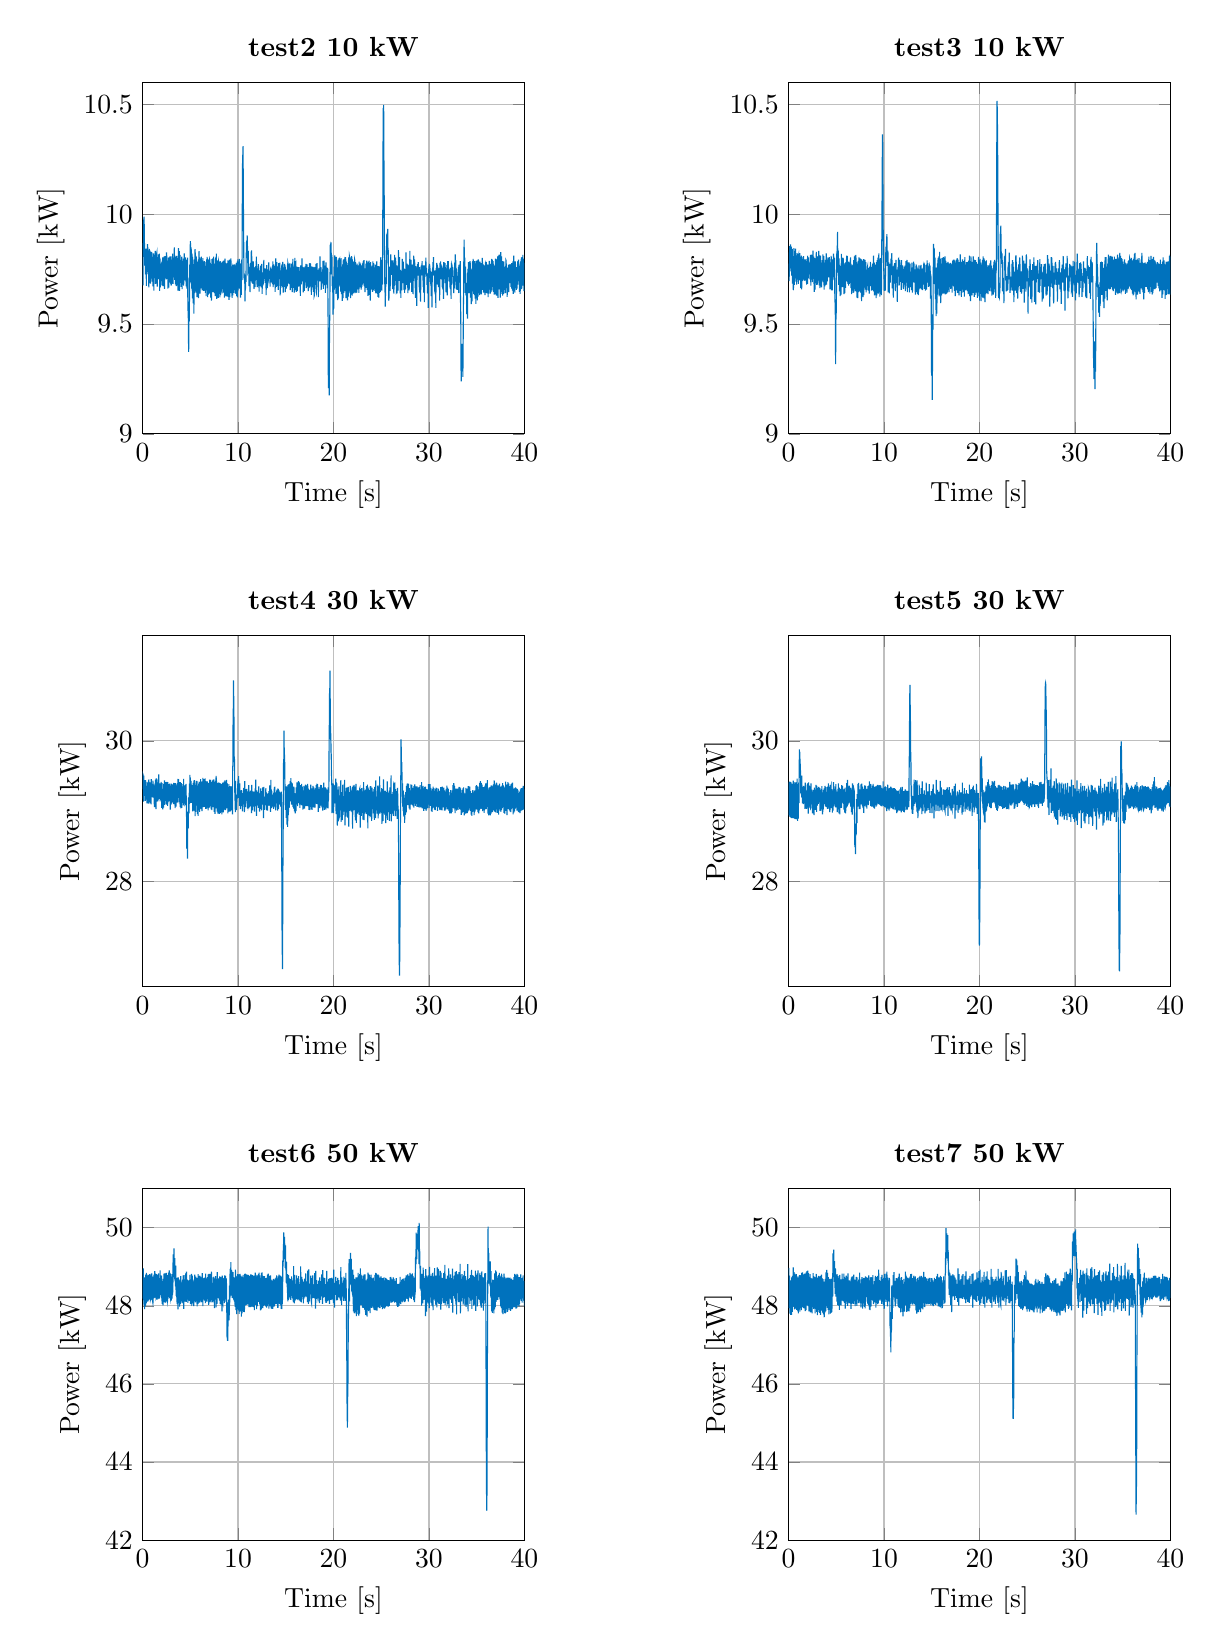
\begin{tikzpicture}

\begin{axis}[%
width=0.4\textwidth,
height=1.757in,
at={(0.953in,6.546in)},
scale only axis,
xmin=0,
xmax=40,
xmajorgrids,
xlabel={Time [s]},
ymin=9,
ymax=10.6,
ymajorgrids,
ylabel={Power [kW]},
axis background/.style={fill=white},
title style={font=\bfseries},
title={test2 10 kW}
]
\addplot [color=mycolor1,solid,forget plot]
  table[row sep=crcr]{%
0.016	9.75384003447836\\
0.032	9.72224233953343\\
0.048	9.67578178452645\\
0.064	9.80121904978439\\
0.08	9.87219186202649\\
0.096	9.95652586693793\\
0.112	9.97533896329203\\
0.128	9.93500361490415\\
0.144	9.96097386080496\\
0.16	9.98965713774721\\
0.176	9.9470051417902\\
0.192	9.91069410913145\\
0.208	9.81245405508609\\
0.224	9.76629516226322\\
0.24	9.83395864111526\\
0.256	9.82235288959759\\
0.272	9.82936738407626\\
0.288	9.80661288868812\\
0.304	9.72684036412854\\
0.32	9.7544122798466\\
0.336	9.8336127216621\\
0.352	9.8239968457724\\
0.368	9.84308390142523\\
0.384	9.75325105013317\\
0.4	9.67449761389755\\
0.416	9.77006848186561\\
0.432	9.78560640290492\\
0.448	9.79947482024814\\
0.464	9.7818549626973\\
0.48	9.72803702747719\\
0.496	9.75175694145649\\
0.512	9.86389039687223\\
0.528	9.85935220250752\\
0.544	9.84733452428943\\
0.56	9.77863473388125\\
0.576	9.7376479295002\\
0.592	9.820350713146\\
0.608	9.8022206165944\\
0.624	9.83551313310202\\
0.64	9.78944959530364\\
0.656	9.6677106226831\\
0.672	9.75439811241214\\
0.688	9.79956163057353\\
0.704	9.81077896956719\\
0.72	9.84277876810497\\
0.736	9.71090354695904\\
0.752	9.68732707395023\\
0.768	9.77474762000624\\
0.784	9.77697819343233\\
0.8	9.83390635143664\\
0.816	9.75730463985773\\
0.832	9.6842351306449\\
0.848	9.76914465880115\\
0.864	9.81447406479256\\
0.88	9.80636371224152\\
0.896	9.79410797972937\\
0.912	9.70754512318711\\
0.928	9.71956848370023\\
0.944	9.82867692746059\\
0.96	9.80748195182228\\
0.976	9.8253614328333\\
0.992	9.75591091523834\\
1.008	9.69340131377778\\
1.024	9.76909696323246\\
1.04	9.76856239184365\\
1.056	9.8059513051427\\
1.072	9.7908080649587\\
1.088	9.67154961572403\\
1.104	9.6983218049443\\
1.12	9.76503967874899\\
1.136	9.78810235247455\\
1.152	9.82245198679759\\
1.168	9.72929325755392\\
1.184	9.65227049632484\\
1.2	9.74352437194441\\
1.216	9.76735420506382\\
1.232	9.8020131519152\\
1.248	9.77731222917597\\
1.264	9.72344447272439\\
1.28	9.72456102250827\\
1.296	9.79517681811561\\
1.312	9.8176113571295\\
1.328	9.83351625699398\\
1.344	9.74493394439452\\
1.36	9.68317316268102\\
1.376	9.75804225581721\\
1.392	9.77108753031015\\
1.408	9.81935208168336\\
1.424	9.78254788508448\\
1.44	9.6854379896821\\
1.456	9.75891560831653\\
1.472	9.81630152390037\\
1.488	9.82369652150978\\
1.504	9.82708498029416\\
1.52	9.71311307482162\\
1.536	9.67083369369644\\
1.552	9.76092212326703\\
1.568	9.76563363028782\\
1.584	9.80494789329895\\
1.6	9.75229344129662\\
1.616	9.70368104004577\\
1.632	9.7557986317975\\
1.648	9.76649411442132\\
1.664	9.81675368374415\\
1.68	9.81226899651138\\
1.696	9.70613541936786\\
1.712	9.72335357975608\\
1.728	9.79147350557944\\
1.744	9.75854642544653\\
1.76	9.82089003898709\\
1.776	9.74534477575435\\
1.792	9.65139716169425\\
1.808	9.76134172053016\\
1.824	9.73788983927082\\
1.84	9.754495433354\\
1.856	9.74851076898971\\
1.872	9.66701429483069\\
1.888	9.71994452059523\\
1.904	9.76821264425761\\
1.92	9.7808659072761\\
1.936	9.77663693436011\\
1.952	9.72166343645112\\
1.968	9.70078994869748\\
1.984	9.7582771379453\\
2	9.73075767416289\\
2.016	9.78057927704116\\
2.032	9.74046116556135\\
2.048	9.67619195380271\\
2.064	9.74066995937227\\
2.08	9.77747426240939\\
2.096	9.75326386956172\\
2.112	9.80323935294874\\
2.128	9.72097266802869\\
2.144	9.67290670635854\\
2.16	9.79216314171084\\
2.176	9.77559617002376\\
2.192	9.78897000006149\\
2.208	9.75877949670343\\
2.224	9.69876652310783\\
2.24	9.78319582634043\\
2.256	9.79592729366116\\
2.272	9.80834960985147\\
2.288	9.75126053546008\\
2.304	9.6607480587091\\
2.32	9.72278278963789\\
2.336	9.7760519226266\\
2.352	9.76628402919903\\
2.368	9.80970735084036\\
2.384	9.74285784958013\\
2.4	9.70917767317628\\
2.416	9.80348893746221\\
2.432	9.78915139532669\\
2.448	9.78171019236971\\
2.464	9.77740434170662\\
2.48	9.70310284649906\\
2.496	9.72813703339519\\
2.512	9.82632996681331\\
2.528	9.81211740976482\\
2.544	9.80473906422476\\
2.56	9.72184777679382\\
2.576	9.7054868813425\\
2.592	9.78884279086589\\
2.608	9.74799160478591\\
2.624	9.77972751214331\\
2.64	9.74522479914495\\
2.656	9.66099029685314\\
2.672	9.76928739915458\\
2.688	9.77561466059971\\
2.704	9.77149399232137\\
2.72	9.8026358429891\\
2.736	9.6884763683814\\
2.752	9.66578367137872\\
2.768	9.7595708265154\\
2.784	9.7381571021012\\
2.8	9.80350110655005\\
2.816	9.7431065422126\\
2.832	9.69080104499577\\
2.848	9.76430048246663\\
2.864	9.79055852324964\\
2.88	9.80780208551384\\
2.896	9.76114698282313\\
2.912	9.69101697468981\\
2.928	9.6889251854147\\
2.944	9.7734411332311\\
2.96	9.75894992740548\\
2.976	9.80864613003013\\
2.992	9.76041964522831\\
3.008	9.6765289853299\\
3.024	9.76832390634685\\
3.04	9.75811675404676\\
3.056	9.78244861628229\\
3.072	9.76834684752549\\
3.088	9.68383511392272\\
3.104	9.69441852087046\\
3.12	9.77297396311311\\
3.136	9.7737668859011\\
3.152	9.82027734481295\\
3.168	9.7224165648079\\
3.184	9.68310189996094\\
3.2	9.75085194489717\\
3.216	9.73962915596271\\
3.232	9.78839790501684\\
3.248	9.78542600845486\\
3.264	9.71250098090591\\
3.28	9.76536165420619\\
3.296	9.77663828874846\\
3.312	9.79709821358724\\
3.328	9.84970225733402\\
3.344	9.75521859955531\\
3.36	9.70080685465713\\
3.376	9.78205389127935\\
3.392	9.75529447229542\\
3.408	9.81085081352933\\
3.424	9.77668605731882\\
3.44	9.68120784390567\\
3.456	9.73859784337986\\
3.472	9.75405181708348\\
3.488	9.78909632976728\\
3.504	9.78555231273791\\
3.52	9.68834046672583\\
3.536	9.67336514685741\\
3.552	9.77765544804068\\
3.568	9.78751402201467\\
3.584	9.81010205400685\\
3.6	9.74885267572168\\
3.616	9.69460472796601\\
3.632	9.74639118918267\\
3.648	9.76189064859991\\
3.664	9.79139898373826\\
3.68	9.77074137958608\\
3.696	9.65265380728659\\
3.712	9.67640115762563\\
3.728	9.77719139393798\\
3.744	9.79685700904624\\
3.76	9.84552503096645\\
3.776	9.75280730675241\\
3.792	9.65289936196858\\
3.808	9.7602694156384\\
3.824	9.77848871265382\\
3.84	9.8319491563402\\
3.856	9.76970567850529\\
3.872	9.65066980872916\\
3.888	9.70892784537204\\
3.904	9.74883296313142\\
3.92	9.8107353243572\\
3.936	9.81497527833254\\
3.952	9.69994626353111\\
3.968	9.68802164945116\\
3.984	9.72051083618403\\
4	9.73175573605821\\
4.016	9.79262862938752\\
4.032	9.75689894870473\\
4.048	9.66941653717566\\
4.064	9.70712973664548\\
4.08	9.7673266030683\\
4.096	9.77586234439691\\
4.112	9.80672478070228\\
4.128	9.71619615134894\\
4.144	9.65892630358525\\
4.16	9.76004533520057\\
4.176	9.74871523914016\\
4.192	9.77953268630376\\
4.208	9.76319940427778\\
4.224	9.6801238565615\\
4.24	9.74797556808652\\
4.256	9.74867066282232\\
4.272	9.79776378664783\\
4.288	9.77637740426822\\
4.304	9.67524780890427\\
4.32	9.69793153765261\\
4.336	9.75506260000012\\
4.352	9.756081982046\\
4.368	9.82154843811665\\
4.384	9.76247500342442\\
4.4	9.69936180227614\\
4.416	9.77534103329805\\
4.432	9.79240355982466\\
4.448	9.77631352791201\\
4.464	9.75711591091021\\
4.48	9.71097428059191\\
4.496	9.70743150667027\\
4.512	9.80374858805184\\
4.528	9.78002878807155\\
4.544	9.77689301594248\\
4.56	9.71254880723436\\
4.576	9.67221014819278\\
4.592	9.76167358903187\\
4.608	9.74838763435978\\
4.624	9.78229570107428\\
4.64	9.7546620384294\\
4.656	9.66136729771804\\
4.672	9.76539549296875\\
4.688	9.79331481124689\\
4.704	9.76500053584171\\
4.72	9.80249338726614\\
4.736	9.64433337603416\\
4.752	9.55996836438299\\
4.768	9.58934998339639\\
4.784	9.52754312893673\\
4.8	9.55622413694493\\
4.816	9.41910850983131\\
4.832	9.37333397703853\\
4.848	9.48554859785293\\
4.864	9.52392370435503\\
4.88	9.60265272547496\\
4.896	9.51208194474878\\
4.912	9.59949599361173\\
4.928	9.74935784036863\\
4.944	9.77078205320493\\
4.96	9.76530444015742\\
4.976	9.68981777941782\\
4.992	9.83566297345748\\
5.008	9.87805697842979\\
5.024	9.8616378670987\\
5.04	9.80664824068669\\
5.056	9.73840833457129\\
5.072	9.84892880173447\\
5.088	9.84296916178917\\
5.104	9.83605999529186\\
5.12	9.78435262731199\\
5.136	9.66164922730027\\
5.152	9.79709555660822\\
5.168	9.8222417490094\\
5.184	9.81047138668098\\
5.2	9.7441624453252\\
5.216	9.61750248456308\\
5.232	9.74073864871775\\
5.248	9.80618411548771\\
5.264	9.76025404334564\\
5.28	9.76183547544932\\
5.296	9.59444072278255\\
5.312	9.64467313547522\\
5.328	9.73106322841793\\
5.344	9.70449685158154\\
5.36	9.70445527250184\\
5.376	9.54723949823673\\
5.392	9.63367876434133\\
5.408	9.7630495145089\\
5.424	9.76707405009589\\
5.44	9.79416526314127\\
5.456	9.64111576189033\\
5.472	9.7324020457653\\
5.488	9.83218710598014\\
5.504	9.84150942741364\\
5.52	9.81730966842977\\
5.536	9.64947226339798\\
5.552	9.70527378401299\\
5.568	9.78791642345643\\
5.584	9.79180742797244\\
5.6	9.78591590945176\\
5.616	9.64364829455248\\
5.632	9.69602048782525\\
5.648	9.78469367621853\\
5.664	9.79139797842688\\
5.68	9.7866303809822\\
5.696	9.62312578866764\\
5.712	9.6660321738263\\
5.728	9.76633601309367\\
5.744	9.76224558551106\\
5.76	9.78376254323507\\
5.776	9.62425626971803\\
5.792	9.66482299465601\\
5.808	9.74256260502387\\
5.824	9.76441843138338\\
5.84	9.76944146074688\\
5.856	9.61792985618698\\
5.872	9.6680168456791\\
5.888	9.79130946849868\\
5.904	9.80411967560987\\
5.92	9.8324661858311\\
5.936	9.67452419188012\\
5.952	9.72059571807752\\
5.968	9.78127783621012\\
5.984	9.77593069704461\\
6	9.80362855728663\\
6.016	9.63830219937069\\
6.032	9.70241514337758\\
6.048	9.77995848630655\\
6.064	9.77959679478619\\
6.08	9.79650231177556\\
6.096	9.66312533014559\\
6.112	9.71249667622196\\
6.128	9.79068702692532\\
6.144	9.78076148710286\\
6.16	9.80750884238918\\
6.176	9.6734540358911\\
6.192	9.70443971801424\\
6.208	9.77887899778036\\
6.224	9.74941819739194\\
6.24	9.79041685858865\\
6.256	9.65305451129282\\
6.272	9.67291379352553\\
6.288	9.74968084065864\\
6.304	9.77304586018094\\
6.32	9.79997021795435\\
6.336	9.65970184396172\\
6.352	9.7064712317771\\
6.368	9.76707698650286\\
6.384	9.75623506258195\\
6.4	9.78391050652008\\
6.416	9.65151677710871\\
6.432	9.71861905498837\\
6.448	9.76965526667305\\
6.464	9.75817793028987\\
6.48	9.78670796348903\\
6.496	9.6522033252773\\
6.512	9.69563733485965\\
6.528	9.76464407064486\\
6.544	9.75707738874997\\
6.56	9.78292028355082\\
6.576	9.64264084636739\\
6.592	9.69968644486741\\
6.608	9.75914692025694\\
6.624	9.74189055498083\\
6.64	9.75802528056517\\
6.656	9.62735648630177\\
6.672	9.68588206669625\\
6.688	9.76320373842311\\
6.704	9.75390243125532\\
6.72	9.79440916366291\\
6.736	9.65363684929101\\
6.752	9.72507066754827\\
6.768	9.80603038847067\\
6.784	9.77362714242588\\
6.8	9.76147932987578\\
6.816	9.62221513799393\\
6.832	9.66022647383825\\
6.848	9.7598559581807\\
6.864	9.7711229656821\\
6.88	9.78656809454811\\
6.896	9.63470534420203\\
6.912	9.70710192452822\\
6.928	9.78901055595452\\
6.944	9.78895652509853\\
6.96	9.79494555087125\\
6.976	9.63867756855507\\
6.992	9.69346408724578\\
7.008	9.77493810326166\\
7.024	9.79449626472978\\
7.04	9.79198605451226\\
7.056	9.64002737026565\\
7.072	9.70542147784317\\
7.088	9.77826551009792\\
7.104	9.76648492593706\\
7.12	9.77294352366831\\
7.136	9.62043473766439\\
7.152	9.67809243773929\\
7.168	9.75727522437833\\
7.184	9.75997465590175\\
7.2	9.76980755100468\\
7.216	9.60662497212189\\
7.232	9.66050525440705\\
7.248	9.72493599410641\\
7.264	9.74689626330379\\
7.28	9.79533240208712\\
7.296	9.65188439409069\\
7.312	9.69031479593305\\
7.328	9.7530209251235\\
7.344	9.76618012522431\\
7.36	9.79947615887249\\
7.376	9.64594503528464\\
7.392	9.69272915788877\\
7.408	9.76579932818937\\
7.424	9.77650440084664\\
7.44	9.80688475463205\\
7.456	9.66274733454412\\
7.472	9.70336363299096\\
7.488	9.77483968443898\\
7.504	9.76237493571969\\
7.52	9.77247782856416\\
7.536	9.64084880431892\\
7.552	9.6929238962532\\
7.568	9.77074824048932\\
7.584	9.75906639215787\\
7.6	9.76108947025161\\
7.616	9.6268806545849\\
7.632	9.71557183370151\\
7.648	9.80281438540317\\
7.664	9.77911961977262\\
7.68	9.74066410630501\\
7.696	9.62979237400358\\
7.712	9.73628831359382\\
7.728	9.82095742428878\\
7.744	9.77678565165574\\
7.76	9.7466479102713\\
7.776	9.61449841097058\\
7.792	9.71414811878241\\
7.808	9.79041035353675\\
7.824	9.750627827476\\
7.84	9.73873593385352\\
7.856	9.62021510090799\\
7.872	9.71288875339181\\
7.888	9.78841015564222\\
7.904	9.76362111289935\\
7.92	9.74802636309706\\
7.936	9.6189325730262\\
7.952	9.70038598227397\\
7.968	9.7841084332891\\
7.984	9.78053192027757\\
8	9.75538330826047\\
8.016	9.63777241761444\\
8.032	9.71865973877079\\
8.048	9.77944154345517\\
8.064	9.78465988433767\\
8.08	9.76675962221999\\
8.096	9.62155710594925\\
8.112	9.71888696262365\\
8.128	9.77644540168862\\
8.144	9.78125184320091\\
8.16	9.78593248495914\\
8.176	9.63200729960023\\
8.192	9.7155210302695\\
8.208	9.77919463319145\\
8.224	9.77434860129667\\
8.24	9.76301271926435\\
8.256	9.6482682676321\\
8.272	9.70760291867189\\
8.288	9.75602957917064\\
8.304	9.76104461055753\\
8.32	9.7799799247775\\
8.336	9.63983098004313\\
8.352	9.6939494457812\\
8.368	9.74922343243356\\
8.384	9.75268248284483\\
8.4	9.78457897265238\\
8.416	9.65975699561353\\
8.432	9.68802732808446\\
8.448	9.74348855516798\\
8.464	9.75274723719607\\
8.48	9.78916977891094\\
8.496	9.64284678372251\\
8.512	9.67834296626376\\
8.528	9.74012714378587\\
8.544	9.77490095909051\\
8.56	9.78826332630252\\
8.576	9.62006250316151\\
8.592	9.66006926193416\\
8.608	9.74701059036239\\
8.624	9.7888006855462\\
8.64	9.79798464283092\\
8.656	9.62630931343958\\
8.672	9.68188075447359\\
8.688	9.74426984047149\\
8.704	9.77826063836721\\
8.72	9.76754448200494\\
8.736	9.63011414215884\\
8.752	9.6846843477977\\
8.768	9.7653370852809\\
8.784	9.77152748446974\\
8.8	9.77666519065944\\
8.816	9.62561232395996\\
8.832	9.69211825335367\\
8.848	9.75511524059063\\
8.864	9.77676167818457\\
8.88	9.77232861020113\\
8.896	9.6309354922966\\
8.912	9.69524619340209\\
8.928	9.76381673806824\\
8.944	9.79010503824962\\
8.96	9.74234208210846\\
8.976	9.62384032128789\\
8.992	9.68958592854174\\
9.008	9.75632455884955\\
9.024	9.78266555402201\\
9.04	9.74587288575469\\
9.056	9.61007417607664\\
9.072	9.68678381816037\\
9.088	9.76732871804432\\
9.104	9.79368035693844\\
9.12	9.75523355691977\\
9.136	9.62293656849868\\
9.152	9.70380689672285\\
9.168	9.76487923472975\\
9.184	9.79013508396378\\
9.2	9.75764695841614\\
9.216	9.64594809940304\\
9.232	9.72344615389213\\
9.248	9.79913425772582\\
9.264	9.78464075556788\\
9.28	9.76362852040979\\
9.296	9.64056763060146\\
9.312	9.72489991174327\\
9.328	9.76242787011189\\
9.344	9.75836451514239\\
9.36	9.7388020460958\\
9.376	9.61915676196895\\
9.392	9.70109140365138\\
9.408	9.74286712261944\\
9.424	9.75578776445349\\
9.44	9.75214436503031\\
9.456	9.63027742556225\\
9.472	9.70770527174283\\
9.488	9.74621598579035\\
9.504	9.76971320797204\\
9.52	9.74470392296779\\
9.536	9.6421379577973\\
9.552	9.70695435548572\\
9.568	9.76343101888829\\
9.584	9.76458705946802\\
9.6	9.77219681346792\\
9.616	9.65409788180615\\
9.632	9.70106687762367\\
9.648	9.75050162993513\\
9.664	9.76263422413562\\
9.68	9.74604985547907\\
9.696	9.64022044483105\\
9.712	9.7021490128595\\
9.728	9.75885381871329\\
9.744	9.76272834288652\\
9.76	9.76539819733209\\
9.776	9.63721796440707\\
9.792	9.700956871026\\
9.808	9.7520510492081\\
9.824	9.76913503765283\\
9.84	9.74784609407228\\
9.856	9.6275858470419\\
9.872	9.69830295552395\\
9.888	9.74823605242325\\
9.904	9.77762174990437\\
9.92	9.74870018236947\\
9.936	9.62217117176652\\
9.952	9.72510251124301\\
9.968	9.77277597873965\\
9.984	9.794312943119\\
10	9.73343103365464\\
10.016	9.65333997474708\\
10.032	9.74191472240359\\
10.048	9.78446633328838\\
10.064	9.78032463121185\\
10.08	9.74644486408781\\
10.096	9.66275518800411\\
10.112	9.73392171398329\\
10.128	9.77240262613169\\
10.144	9.79660828291759\\
10.16	9.7694837584179\\
10.176	9.66140495587525\\
10.192	9.7429628838093\\
10.208	9.77659313325767\\
10.224	9.77211502717406\\
10.24	9.75568300074419\\
10.256	9.62079550605005\\
10.272	9.70098402525894\\
10.288	9.71759729905089\\
10.304	9.74619834629806\\
10.32	9.73555656729345\\
10.336	9.63252725508811\\
10.352	9.72385729871334\\
10.368	9.77149307244938\\
10.384	9.79322895991683\\
10.4	9.77368857174287\\
10.416	9.70032611860307\\
10.432	9.86107465709323\\
10.448	10.0436740306313\\
10.464	10.1498161636003\\
10.48	10.2703159183924\\
10.496	10.2206891298103\\
10.512	10.2393411913477\\
10.528	10.3097597810426\\
10.544	10.1943992860295\\
10.56	10.050153129678\\
10.576	9.99603650167333\\
10.592	9.88953518248253\\
10.608	9.78773451325689\\
10.624	9.71836770992275\\
10.64	9.70300794335048\\
10.656	9.72676546927254\\
10.672	9.71248660074166\\
10.688	9.71737579344831\\
10.704	9.72456223740808\\
10.72	9.62688327153712\\
10.736	9.60308451444389\\
10.752	9.65395183378308\\
10.768	9.65624119995105\\
10.784	9.66432117187044\\
10.8	9.72409350160451\\
10.816	9.70969149199041\\
10.832	9.6925415297882\\
10.848	9.77737405269052\\
10.864	9.81997253022005\\
10.88	9.84462756531688\\
10.896	9.87940743161303\\
10.912	9.86735357617072\\
10.928	9.86794766667657\\
10.944	9.82308026333386\\
10.96	9.90421237594357\\
10.976	9.84502419285743\\
10.992	9.84854914653439\\
11.008	9.82834895724389\\
11.024	9.77944339135147\\
11.04	9.74130410139467\\
11.056	9.74469582569431\\
11.072	9.83297939846921\\
11.088	9.76469533071925\\
11.104	9.74552395730936\\
11.12	9.77497817014202\\
11.136	9.70555232437891\\
11.152	9.67316682404206\\
11.168	9.70313842805495\\
11.184	9.73409465143431\\
11.2	9.72646216303938\\
11.216	9.76010116771311\\
11.232	9.70613440677529\\
11.248	9.65503320790918\\
11.264	9.64520911169743\\
11.28	9.73238612205644\\
11.296	9.73505220581533\\
11.312	9.74552673528353\\
11.328	9.77884193723805\\
11.344	9.72463695214549\\
11.36	9.69541770307811\\
11.376	9.74950263908872\\
11.392	9.83204169566144\\
11.408	9.82652181111923\\
11.424	9.83590994871494\\
11.44	9.78495702221819\\
11.456	9.72704861184605\\
11.472	9.6859937644303\\
11.488	9.74109483028231\\
11.504	9.74500594659781\\
11.52	9.73421863551691\\
11.536	9.73954876471038\\
11.552	9.70644715040119\\
11.568	9.68359497094639\\
11.584	9.69075505618987\\
11.6	9.78512891964242\\
11.616	9.73424298012779\\
11.632	9.75570289558832\\
11.648	9.75616239146615\\
11.664	9.67377704686719\\
11.68	9.66081188951512\\
11.696	9.70123241862122\\
11.712	9.74013683691969\\
11.728	9.72033098520933\\
11.744	9.75812725633646\\
11.76	9.73408991095386\\
11.776	9.67463757609945\\
11.792	9.66854521125934\\
11.808	9.73462870086279\\
11.824	9.75236231950687\\
11.84	9.7549066609756\\
11.856	9.76310510467711\\
11.872	9.72974785550668\\
11.888	9.70165648871274\\
11.904	9.74396080544205\\
11.92	9.80696749500819\\
11.936	9.76864591817161\\
11.952	9.77390145677494\\
11.968	9.73712661852976\\
11.984	9.70034087000423\\
12	9.66793533089413\\
12.016	9.74710651172472\\
12.032	9.72551691084586\\
12.048	9.7117273644418\\
12.064	9.74483496572199\\
12.08	9.71679869257524\\
12.096	9.6818605476656\\
12.112	9.68404165955163\\
12.128	9.77260914088046\\
12.144	9.71387454621829\\
12.16	9.72493011269301\\
12.176	9.73441266195534\\
12.192	9.70337148288958\\
12.208	9.64758518465031\\
12.224	9.70212698968191\\
12.24	9.73506810604948\\
12.256	9.73879920547216\\
12.272	9.74402286694015\\
12.288	9.72756856420158\\
12.304	9.67258057705747\\
12.32	9.69212424959101\\
12.336	9.76557918349056\\
12.352	9.72532585523324\\
12.368	9.74680707274235\\
12.384	9.74962443960611\\
12.4	9.71758653042248\\
12.416	9.66767478473777\\
12.432	9.73799884222972\\
12.448	9.75538546041123\\
12.464	9.73292078103402\\
12.48	9.77453591189732\\
12.496	9.75926260506966\\
12.512	9.69551624360452\\
12.528	9.63806607960924\\
12.544	9.72437286225801\\
12.56	9.69248374886342\\
12.576	9.69187745882192\\
12.592	9.73487732763533\\
12.608	9.72587901333367\\
12.624	9.67696309049305\\
12.64	9.68468976737413\\
12.656	9.71803125648572\\
12.672	9.72749431169625\\
12.688	9.76172432963426\\
12.704	9.79185869497325\\
12.72	9.73032445994765\\
12.736	9.71051004880064\\
12.752	9.73417294154841\\
12.768	9.71692313620079\\
12.784	9.70611068128399\\
12.8	9.7538995745995\\
12.816	9.7430724217809\\
12.832	9.69596298485069\\
12.848	9.68830215917824\\
12.864	9.73771171172677\\
12.88	9.6952380492554\\
12.896	9.71935344247104\\
12.912	9.75211527588466\\
12.928	9.69772526524696\\
12.944	9.63219009749605\\
12.96	9.68636485755314\\
12.976	9.72749178310278\\
12.992	9.72949993785106\\
13.008	9.76877364387126\\
13.024	9.76051889691518\\
13.04	9.72357982918193\\
13.056	9.66364909797794\\
13.072	9.72610325173817\\
13.088	9.70287153945522\\
13.104	9.7249108982368\\
13.12	9.74861221901759\\
13.136	9.70046826101853\\
13.152	9.69263472720954\\
13.168	9.6969641847429\\
13.184	9.74169903817763\\
13.2	9.71431512836331\\
13.216	9.78113281710244\\
13.232	9.76863677503916\\
13.248	9.72001146777419\\
13.264	9.7068844161578\\
13.28	9.74142278315058\\
13.296	9.72399333680272\\
13.312	9.70574563536571\\
13.328	9.72897427136219\\
13.344	9.72068536813315\\
13.36	9.67034784654024\\
13.376	9.71516627883793\\
13.392	9.73582386693783\\
13.408	9.72876415946695\\
13.424	9.74306465525353\\
13.44	9.76120552966147\\
13.456	9.72879867882361\\
13.472	9.69045162458948\\
13.488	9.745648466954\\
13.504	9.71424164126957\\
13.52	9.72014686012232\\
13.536	9.75203102973303\\
13.552	9.7358290776588\\
13.568	9.71635191069304\\
13.584	9.68754393171114\\
13.6	9.73222206641411\\
13.616	9.68160611534702\\
13.632	9.72564368900355\\
13.648	9.78536348189011\\
13.664	9.73111206985635\\
13.68	9.66805567680563\\
13.696	9.70046274787349\\
13.712	9.74452964400366\\
13.728	9.73563672075847\\
13.744	9.77226647341785\\
13.76	9.75562650893547\\
13.776	9.70749836796355\\
13.792	9.68097106259045\\
13.808	9.73941198431504\\
13.824	9.73817910191223\\
13.84	9.75683594986518\\
13.856	9.76463627863122\\
13.872	9.73368937427781\\
13.888	9.64690777433021\\
13.904	9.69252854577305\\
13.92	9.74058984830642\\
13.936	9.72996534089114\\
13.952	9.7988768768446\\
13.968	9.7722535775354\\
13.984	9.7082836495784\\
14	9.66958521649232\\
14.016	9.74687143151865\\
14.032	9.7220581786882\\
14.048	9.74197425471392\\
14.064	9.78198307420595\\
14.08	9.74879645456835\\
14.096	9.68096025535216\\
14.112	9.67293916350096\\
14.128	9.73940873017135\\
14.144	9.73964325146998\\
14.16	9.76232611957778\\
14.176	9.75365181250674\\
14.192	9.68207964605866\\
14.208	9.65528826148319\\
14.224	9.70424382941905\\
14.24	9.73237022460635\\
14.256	9.75845943013619\\
14.272	9.7774395938093\\
14.288	9.76545439398645\\
14.304	9.70928448998869\\
14.32	9.70859926606875\\
14.336	9.76455497650786\\
14.352	9.73911138333958\\
14.368	9.75674687013715\\
14.384	9.77972131089173\\
14.4	9.68253429239454\\
14.416	9.63123951216236\\
14.432	9.69102587938109\\
14.448	9.71263071392765\\
14.464	9.71285102267074\\
14.48	9.73975614177024\\
14.496	9.74372554679592\\
14.512	9.69812973208647\\
14.528	9.67238299454391\\
14.544	9.75560725378874\\
14.56	9.75117194898172\\
14.576	9.75792908772514\\
14.592	9.77142045274369\\
14.608	9.6987500163935\\
14.624	9.67468784446623\\
14.64	9.67620510372454\\
14.656	9.76751204673156\\
14.672	9.7327905925722\\
14.688	9.78311500906272\\
14.704	9.73269813958148\\
14.72	9.65859346372202\\
14.736	9.64297028046993\\
14.752	9.69677076841633\\
14.768	9.70562093825006\\
14.784	9.72735061773685\\
14.8	9.75841368879966\\
14.816	9.71926425236862\\
14.832	9.66892352036772\\
14.848	9.71284018337165\\
14.864	9.77387913990396\\
14.88	9.75473118677218\\
14.896	9.76949474063638\\
14.912	9.72505865995224\\
14.928	9.70302508319879\\
14.944	9.64570217704925\\
14.96	9.72480814271987\\
14.976	9.73163627632979\\
14.992	9.74429104303342\\
15.008	9.739728776858\\
15.024	9.73344960040979\\
15.04	9.69192405488014\\
15.056	9.66181162024673\\
15.072	9.71931314430357\\
15.088	9.70339620353225\\
15.104	9.73289899284359\\
15.12	9.7306162413612\\
15.136	9.69889160970822\\
15.152	9.67176082683771\\
15.168	9.69677125089174\\
15.184	9.77070938207819\\
15.2	9.75620403258334\\
15.216	9.77852424623491\\
15.232	9.77466344398216\\
15.248	9.70470333404314\\
15.264	9.68548519197136\\
15.28	9.72947625189756\\
15.296	9.75299302517734\\
15.312	9.73501812348465\\
15.328	9.77470828786047\\
15.344	9.72009368020456\\
15.36	9.68234584416536\\
15.376	9.70576818665631\\
15.392	9.7677365040961\\
15.408	9.75355087536552\\
15.424	9.77596212134064\\
15.44	9.74094099987403\\
15.456	9.68294650186492\\
15.472	9.65468635260548\\
15.488	9.72764845605621\\
15.504	9.74299074034386\\
15.52	9.72216776384132\\
15.536	9.75747070295459\\
15.552	9.71314822252355\\
15.568	9.67196940717045\\
15.584	9.66500804906841\\
15.6	9.77488348462194\\
15.616	9.74786469079634\\
15.632	9.76468341064196\\
15.648	9.7537151634619\\
15.664	9.71547630252357\\
15.68	9.64561431789997\\
15.696	9.70658695287957\\
15.712	9.76153083954579\\
15.728	9.75523292861066\\
15.744	9.79632602041056\\
15.76	9.7522420802581\\
15.776	9.68242561866292\\
15.792	9.66475525549757\\
15.808	9.7239775058192\\
15.824	9.71702832556345\\
15.84	9.74126377088325\\
15.856	9.76110273417716\\
15.872	9.70867455541641\\
15.888	9.64353681403368\\
15.904	9.70653569224505\\
15.92	9.7414749937715\\
15.936	9.74707943985596\\
15.952	9.80124142393751\\
15.968	9.76708911161932\\
15.984	9.67771009264539\\
16	9.65489800332785\\
16.016	9.78660725452439\\
16.032	9.78159984471894\\
16.048	9.76645776318543\\
16.064	9.76972097203633\\
16.08	9.68579607480483\\
16.096	9.64700420151344\\
16.112	9.7059753078994\\
16.128	9.75681258806673\\
16.144	9.75636066097069\\
16.16	9.76131102578046\\
16.176	9.74255881595308\\
16.192	9.67906561268073\\
16.208	9.65006492177595\\
16.224	9.68373483799787\\
16.24	9.73557195097078\\
16.256	9.73683536111694\\
16.272	9.75873176294044\\
16.288	9.74764726429034\\
16.304	9.67064027044252\\
16.32	9.67636418860322\\
16.336	9.70529694132254\\
16.352	9.71062073146039\\
16.368	9.73676851380291\\
16.384	9.75914303737684\\
16.4	9.71828845956075\\
16.416	9.67208702731481\\
16.432	9.71800440980156\\
16.448	9.72723889399948\\
16.464	9.71771085289343\\
16.48	9.74254188075691\\
16.496	9.72866510540503\\
16.512	9.68256782883519\\
16.528	9.62875887715722\\
16.544	9.71519815610859\\
16.56	9.7176344355769\\
16.576	9.76749981937127\\
16.592	9.75789989221515\\
16.608	9.71485277390676\\
16.624	9.68070831718734\\
16.64	9.71751980809275\\
16.656	9.75020230971581\\
16.672	9.73205084448333\\
16.688	9.7762678076207\\
16.704	9.79910307858036\\
16.72	9.71831886567661\\
16.736	9.69486640760385\\
16.752	9.73577220592706\\
16.768	9.7105383713219\\
16.784	9.71170016978226\\
16.8	9.76047063863241\\
16.816	9.73143014373661\\
16.832	9.6439221648742\\
16.848	9.67594736942422\\
16.864	9.75680483663351\\
16.88	9.71088003590403\\
16.896	9.7335517038989\\
16.912	9.73283404726685\\
16.928	9.70213723512633\\
16.944	9.65098950948275\\
16.96	9.68095225593066\\
16.976	9.68684467808928\\
16.992	9.69400888164637\\
17.008	9.74246633521592\\
17.024	9.76291653457054\\
17.04	9.7191478779929\\
17.056	9.69081584711131\\
17.072	9.73232134439717\\
17.088	9.70292631318473\\
17.104	9.7513817018773\\
17.12	9.77461879363668\\
17.136	9.71692978508133\\
17.152	9.6634065144785\\
17.168	9.69333109928417\\
17.184	9.7228985625058\\
17.2	9.70887852790271\\
17.216	9.74899342444895\\
17.232	9.77144376408666\\
17.248	9.71144605590963\\
17.264	9.67058951540114\\
17.28	9.70942320359004\\
17.296	9.73000391641632\\
17.312	9.75174693114328\\
17.328	9.75896117887798\\
17.344	9.71809722310105\\
17.36	9.65014944621069\\
17.376	9.65556722958787\\
17.392	9.70503651093\\
17.408	9.68740731649419\\
17.424	9.74629185439449\\
17.44	9.71082068004\\
17.456	9.67601591346561\\
17.472	9.66628431844819\\
17.488	9.77604879181426\\
17.504	9.73970188124557\\
17.52	9.74952002101761\\
17.536	9.77759426002839\\
17.552	9.7435189321189\\
17.568	9.67865275237047\\
17.584	9.67672792672481\\
17.6	9.77503492966561\\
17.616	9.7498775351374\\
17.632	9.7638668222928\\
17.648	9.75663819271635\\
17.664	9.68980975821972\\
17.68	9.63324466553102\\
17.696	9.68413451297491\\
17.712	9.72225960442715\\
17.728	9.74139475816198\\
17.744	9.76159619426554\\
17.76	9.74873181907463\\
17.776	9.67979895340206\\
17.792	9.68266140628228\\
17.808	9.70449458415324\\
17.824	9.70772846719969\\
17.84	9.72341834397865\\
17.856	9.76051319493523\\
17.872	9.7016390161806\\
17.888	9.6463268491291\\
17.904	9.72544519024906\\
17.92	9.75793032048965\\
17.936	9.71821500028456\\
17.952	9.72437352593118\\
17.968	9.72898368220589\\
17.984	9.62889736955955\\
18	9.6314663984348\\
18.016	9.72275697191857\\
18.032	9.7428712252817\\
18.048	9.73621629373607\\
18.064	9.75984426696253\\
18.08	9.71328760802588\\
18.096	9.68504899660019\\
18.112	9.67873428687844\\
18.128	9.75261217872619\\
18.144	9.73291553006622\\
18.16	9.77380160817089\\
18.176	9.72886450478885\\
18.192	9.64536906956233\\
18.208	9.64249221797934\\
18.224	9.7040833040522\\
18.24	9.70464273045909\\
18.256	9.72984783364064\\
18.272	9.7775698930987\\
18.288	9.75257519001201\\
18.304	9.69925409834423\\
18.32	9.72613307439165\\
18.336	9.74720838898992\\
18.352	9.69835196158761\\
18.368	9.72071675089336\\
18.384	9.71872090748245\\
18.4	9.69561086262952\\
18.416	9.62236588525755\\
18.432	9.67022614922356\\
18.448	9.69453549232453\\
18.464	9.71876939915592\\
18.48	9.75345215606098\\
18.496	9.73460910620463\\
18.512	9.69455150225151\\
18.528	9.6994641477435\\
18.544	9.74377390568542\\
18.56	9.71292171899532\\
18.576	9.76073558546827\\
18.592	9.80809348224259\\
18.608	9.7287320889401\\
18.624	9.69421282061779\\
18.64	9.7050797873644\\
18.656	9.74619603883986\\
18.672	9.71215646944298\\
18.688	9.74982621724945\\
18.704	9.75866158372655\\
18.72	9.65930075323489\\
18.736	9.65982145802001\\
18.752	9.73105895055716\\
18.768	9.72432335927429\\
18.784	9.68163081875022\\
18.8	9.71956418142649\\
18.816	9.70496826750873\\
18.832	9.68709634875496\\
18.848	9.73091682846996\\
18.864	9.74710477322311\\
18.88	9.74759599531466\\
18.896	9.78791559535819\\
18.912	9.77912635351723\\
18.928	9.71213031710409\\
18.944	9.6603368633994\\
18.96	9.75039366976018\\
18.976	9.74236509531059\\
18.992	9.74039073798317\\
19.008	9.78908471669519\\
19.024	9.72936211834425\\
19.04	9.67717274145106\\
19.056	9.68977795089678\\
19.072	9.76632343558525\\
19.088	9.71048179521843\\
19.104	9.73615408903326\\
19.12	9.74888928275434\\
19.136	9.69757241153833\\
19.152	9.64186713412096\\
19.168	9.69368834061602\\
19.184	9.74652701871699\\
19.2	9.74893860559636\\
19.216	9.78048862644814\\
19.232	9.7482594448712\\
19.248	9.68683960067097\\
19.264	9.67934205545855\\
19.28	9.75768640160297\\
19.296	9.72108462118382\\
19.312	9.72858148411186\\
19.328	9.74321714420697\\
19.344	9.70290148844378\\
19.36	9.66382487651198\\
19.376	9.72632179005768\\
19.392	9.7556476397807\\
19.408	9.66706627518733\\
19.424	9.59437924701769\\
19.44	9.44058207212387\\
19.456	9.26952467507277\\
19.472	9.2087086794823\\
19.488	9.26181690963334\\
19.504	9.25907343072214\\
19.52	9.3084447228359\\
19.536	9.23015508853717\\
19.552	9.17566513041205\\
19.568	9.35886460272427\\
19.584	9.46799971770611\\
19.6	9.54156118083436\\
19.616	9.5153107661424\\
19.632	9.68249561034482\\
19.648	9.79463863907247\\
19.664	9.85923448088016\\
19.68	9.86136444603209\\
19.696	9.77767226225188\\
19.712	9.84725249155811\\
19.728	9.8348320459427\\
19.744	9.87241953434604\\
19.76	9.82214257126636\\
19.776	9.72608404633504\\
19.792	9.75685737763931\\
19.808	9.77808542909127\\
19.824	9.81483013203367\\
19.84	9.80335513100739\\
19.856	9.69011105560891\\
19.872	9.67263720213499\\
19.888	9.71701015825356\\
19.904	9.69930389743352\\
19.92	9.71555031336108\\
19.936	9.57081989671306\\
19.952	9.54313429261598\\
19.968	9.65590763595922\\
19.984	9.66441624214929\\
20	9.68634928134026\\
20.016	9.57170302467944\\
20.032	9.57353069199912\\
20.048	9.68632328695465\\
20.064	9.73216608917956\\
20.08	9.76157854933256\\
20.096	9.65734453272673\\
20.112	9.69678620358562\\
20.128	9.81251404635397\\
20.144	9.79048407031218\\
20.16	9.76291507384784\\
20.176	9.66409249196122\\
20.192	9.72125738090841\\
20.208	9.79260508737475\\
20.224	9.77599582795374\\
20.24	9.77216789389918\\
20.256	9.63731840679458\\
20.272	9.68153290280677\\
20.288	9.80541368499653\\
20.304	9.7917243540712\\
20.32	9.79818453956583\\
20.336	9.67531901874318\\
20.352	9.69223298529334\\
20.368	9.79001136233834\\
20.384	9.76422788260357\\
20.4	9.74052962586481\\
20.416	9.64990168734348\\
20.432	9.60892784616503\\
20.448	9.72787046565613\\
20.464	9.71577231626929\\
20.48	9.7252780858159\\
20.496	9.61855820148348\\
20.512	9.61983995821604\\
20.528	9.75413487904459\\
20.544	9.77116397146334\\
20.56	9.79819262701447\\
20.576	9.69376211645899\\
20.592	9.67006118686965\\
20.608	9.80037215954583\\
20.624	9.7936681552243\\
20.64	9.79554523832101\\
20.656	9.67640451621825\\
20.672	9.68645814900481\\
20.688	9.77435515164167\\
20.704	9.77620428694824\\
20.72	9.79485416293139\\
20.736	9.69170949135042\\
20.752	9.64771510309241\\
20.768	9.72969293097927\\
20.784	9.75254045720383\\
20.8	9.80014674205315\\
20.816	9.69480232196261\\
20.832	9.63600219688752\\
20.848	9.73432102775772\\
20.864	9.75423769400915\\
20.88	9.76100782854813\\
20.896	9.66529208037508\\
20.912	9.60609410470978\\
20.928	9.72546445951261\\
20.944	9.74756275698684\\
20.96	9.772026212182\\
20.976	9.66735690427096\\
20.992	9.61857413546039\\
21.008	9.76050100223789\\
21.024	9.78707661502538\\
21.04	9.79408444844665\\
21.056	9.67199271815739\\
21.072	9.64224559660328\\
21.088	9.76846734106043\\
21.104	9.78148641058303\\
21.12	9.7842409385493\\
21.136	9.66748757530788\\
21.152	9.65056304980744\\
21.168	9.77858188528745\\
21.184	9.79550769287853\\
21.2	9.79378617351314\\
21.216	9.67067828557824\\
21.232	9.6581631392746\\
21.248	9.77611953970886\\
21.264	9.80472558667501\\
21.28	9.79357049832877\\
21.296	9.66551297194093\\
21.312	9.61776970875683\\
21.328	9.77671200585288\\
21.344	9.78453856650667\\
21.36	9.76259418111297\\
21.376	9.65439201320252\\
21.392	9.62020260424107\\
21.408	9.75310370648505\\
21.424	9.76831830499176\\
21.44	9.75667426030615\\
21.456	9.66145795885908\\
21.472	9.60742471270748\\
21.488	9.74378782449628\\
21.504	9.7769473491921\\
21.52	9.75812937291468\\
21.536	9.66725479741645\\
21.552	9.62468266426319\\
21.568	9.77807954014825\\
21.584	9.80394426510276\\
21.6	9.7946174128799\\
21.616	9.66861023429458\\
21.632	9.65537636076361\\
21.648	9.77230963645944\\
21.664	9.81043870751042\\
21.68	9.80667642462082\\
21.696	9.67341910436624\\
21.712	9.64155730020175\\
21.728	9.77383738190748\\
21.744	9.80489287623772\\
21.76	9.78213095139698\\
21.776	9.62700717583349\\
21.792	9.61881324766496\\
21.808	9.77019135380815\\
21.824	9.79895997506266\\
21.84	9.77576655435015\\
21.856	9.65271526537183\\
21.872	9.63457283581645\\
21.888	9.79158306375216\\
21.904	9.80955330773816\\
21.92	9.78014018997808\\
21.936	9.64973462703431\\
21.952	9.63079135269414\\
21.968	9.78160706469773\\
21.984	9.78341756541317\\
22	9.77332108260514\\
22.016	9.64573888246709\\
22.032	9.64820014044044\\
22.048	9.78143090266573\\
22.064	9.78185943520625\\
22.08	9.76067127419618\\
22.096	9.63945729721666\\
22.112	9.66011686727198\\
22.128	9.76479292325676\\
22.144	9.77345326025911\\
22.16	9.76346058452869\\
22.176	9.64504827824961\\
22.192	9.66420789306654\\
22.208	9.79595571462603\\
22.224	9.79302050989053\\
22.24	9.78746150207606\\
22.256	9.65241971963202\\
22.272	9.64076068217345\\
22.288	9.7490413321494\\
22.304	9.78245895259823\\
22.32	9.77414317023156\\
22.336	9.65459075852253\\
22.352	9.64459691680587\\
22.368	9.7514407519163\\
22.384	9.76237885402867\\
22.4	9.76786870665424\\
22.416	9.65219949472801\\
22.432	9.64281803585586\\
22.448	9.74594826312616\\
22.464	9.75829522799463\\
22.48	9.77563260214907\\
22.496	9.67151027986954\\
22.512	9.66004347904373\\
22.528	9.75459918329813\\
22.544	9.75200484102937\\
22.56	9.76748685159831\\
22.576	9.65784848824934\\
22.592	9.66617983186715\\
22.608	9.74244981442961\\
22.624	9.75827162810435\\
22.64	9.75869678447942\\
22.656	9.64264951963516\\
22.672	9.67126202178016\\
22.688	9.7842826070536\\
22.704	9.74880347607368\\
22.72	9.76792180634666\\
22.736	9.66682362865608\\
22.752	9.67325743507934\\
22.768	9.76790387379347\\
22.784	9.75992767674638\\
22.8	9.76257754953085\\
22.816	9.66789304521151\\
22.832	9.67757499088548\\
22.848	9.75395907558319\\
22.864	9.75202011010969\\
22.88	9.75920028002489\\
22.896	9.65639531910652\\
22.912	9.6777175334149\\
22.928	9.75173541735639\\
22.944	9.75651788580679\\
22.96	9.76728531118889\\
22.976	9.66949284035613\\
22.992	9.69929783262789\\
23.008	9.76717631010196\\
23.024	9.72871941508593\\
23.04	9.77628170516937\\
23.056	9.68050155317206\\
23.072	9.71640048532603\\
23.088	9.76881522297125\\
23.104	9.76841857736775\\
23.12	9.7848401355948\\
23.136	9.69377649829339\\
23.152	9.71905809078285\\
23.168	9.78757166347237\\
23.184	9.7704182405971\\
23.2	9.79125429262941\\
23.216	9.67992399893329\\
23.232	9.67142509582476\\
23.248	9.74530705575717\\
23.264	9.73831194555848\\
23.28	9.74931043368099\\
23.296	9.6457363892476\\
23.312	9.65879730913327\\
23.328	9.7530820224128\\
23.344	9.73318724152056\\
23.36	9.74731433022744\\
23.376	9.66555461622532\\
23.392	9.67117461966922\\
23.408	9.77495492053108\\
23.424	9.75666945322905\\
23.44	9.76750677298486\\
23.456	9.66656811361488\\
23.472	9.68196426080791\\
23.488	9.78924855676156\\
23.504	9.77390337522767\\
23.52	9.77865202311385\\
23.536	9.65551670965541\\
23.552	9.67553662087957\\
23.568	9.7797264602402\\
23.584	9.75333406088879\\
23.6	9.75678364672402\\
23.616	9.62818086646874\\
23.632	9.6750384112845\\
23.648	9.78405049212781\\
23.664	9.76940611462384\\
23.68	9.75955712729005\\
23.696	9.64383419284625\\
23.712	9.67650874762495\\
23.728	9.78854134363173\\
23.744	9.77410896322465\\
23.76	9.74662929581556\\
23.776	9.63263488481162\\
23.792	9.65680006679868\\
23.808	9.76382772788833\\
23.824	9.73478710435101\\
23.84	9.72771922873176\\
23.856	9.60652853272643\\
23.872	9.64999750394636\\
23.888	9.78173917778342\\
23.904	9.74167793899337\\
23.92	9.75723698530175\\
23.936	9.65527801589478\\
23.952	9.69495709112365\\
23.968	9.75262388581607\\
23.984	9.74018605397162\\
24	9.76149070159848\\
24.016	9.66337865595626\\
24.032	9.66320471946008\\
24.048	9.76638588110286\\
24.064	9.74155168084991\\
24.08	9.7486916930138\\
24.096	9.64698951405285\\
24.112	9.66582485830221\\
24.128	9.78578848600999\\
24.144	9.73809008640396\\
24.16	9.75718162890125\\
24.176	9.65338142286702\\
24.192	9.66883929062965\\
24.208	9.77781980348344\\
24.224	9.75955802660959\\
24.24	9.75217432005577\\
24.256	9.65879951615357\\
24.272	9.66635327351494\\
24.288	9.75436670789479\\
24.304	9.72988218142874\\
24.32	9.75800031274942\\
24.336	9.65101548753616\\
24.352	9.66470403398535\\
24.368	9.74727647031846\\
24.384	9.75349088788598\\
24.4	9.77094956409833\\
24.416	9.6552518738938\\
24.432	9.65771269749663\\
24.448	9.75032218374928\\
24.464	9.7430493007109\\
24.48	9.76677731303436\\
24.496	9.64175974364137\\
24.512	9.70698537054773\\
24.528	9.78589405127679\\
24.544	9.7604407660233\\
24.56	9.7525912746944\\
24.576	9.63813178567991\\
24.592	9.66717299108774\\
24.608	9.7614781676947\\
24.624	9.74009980783062\\
24.64	9.7446886669398\\
24.656	9.62340708828419\\
24.672	9.65630209595453\\
24.688	9.76401165225432\\
24.704	9.74056403776814\\
24.72	9.74731687829594\\
24.736	9.6204484465919\\
24.752	9.64880694579286\\
24.768	9.74683903645792\\
24.784	9.74462492631377\\
24.8	9.76258264475397\\
24.816	9.6425761458214\\
24.832	9.66046233923308\\
24.848	9.7514006075066\\
24.864	9.76258780676334\\
24.88	9.75456256609708\\
24.896	9.64622755513586\\
24.912	9.65962900910032\\
24.928	9.78069337578758\\
24.944	9.79102765875482\\
24.96	9.80526706619344\\
24.976	9.65213188282021\\
24.992	9.65975583863682\\
25.008	9.76893830933333\\
25.024	9.77263610716071\\
25.04	9.76156557746462\\
25.056	9.65316086864609\\
25.072	9.6585749032652\\
25.088	9.76295299365958\\
25.104	9.7546621134727\\
25.12	9.77682513545441\\
25.136	9.68113895808309\\
25.152	9.78207347885721\\
25.168	10.0759959986037\\
25.184	10.2545817049608\\
25.2	10.4289330359952\\
25.216	10.4845000840782\\
25.232	10.4429184258191\\
25.248	10.4982562877475\\
25.264	10.4526363439083\\
25.28	10.2755709475735\\
25.296	10.168946335189\\
25.312	10.0790588611051\\
25.328	9.92574080057984\\
25.344	9.80095935955604\\
25.36	9.82259041684271\\
25.376	9.66663123838643\\
25.392	9.65251780972748\\
25.408	9.65462264759677\\
25.424	9.57907889874598\\
25.44	9.62665165652531\\
25.456	9.64079530204356\\
25.472	9.68130321755883\\
25.488	9.71285432320166\\
25.504	9.70797886715999\\
25.52	9.68224517283796\\
25.536	9.70941678100665\\
25.552	9.81334517250866\\
25.568	9.87526548791373\\
25.584	9.9082727879019\\
25.6	9.88364933566472\\
25.616	9.91643937348244\\
25.632	9.90957755537969\\
25.648	9.85163486124649\\
25.664	9.84179986417492\\
25.68	9.93335641042907\\
25.696	9.85586429371643\\
25.712	9.81672924883879\\
25.728	9.84676648150401\\
25.744	9.7532094896091\\
25.76	9.69614397466404\\
25.776	9.6629090783841\\
25.792	9.60702798974157\\
25.808	9.61533105031346\\
25.824	9.68040560991435\\
25.84	9.67590319770959\\
25.856	9.71156565573231\\
25.872	9.76197545552151\\
25.888	9.72623528343778\\
25.904	9.68885382505501\\
25.92	9.65074985934651\\
25.936	9.66441989919245\\
25.952	9.70584445158028\\
25.968	9.73135183434986\\
25.984	9.74407550156522\\
26	9.81687169563572\\
26.016	9.75855035910921\\
26.032	9.72447985013689\\
26.048	9.7529179158962\\
26.064	9.74950394410085\\
26.08	9.79032510928782\\
26.096	9.76527647036706\\
26.112	9.7615817369967\\
26.128	9.74480228799134\\
26.144	9.75743963325733\\
26.16	9.75019817172605\\
26.176	9.71575380344613\\
26.192	9.65900873366964\\
26.208	9.69903727490887\\
26.224	9.78977964697934\\
26.24	9.74442275394276\\
26.256	9.66692340737095\\
26.272	9.71798909102698\\
26.288	9.72080435621587\\
26.304	9.66698007650765\\
26.32	9.63896651740943\\
26.336	9.68669300113267\\
26.352	9.65767352921622\\
26.368	9.69918753515153\\
26.384	9.72893444413303\\
26.4	9.81504754860688\\
26.416	9.7654090633589\\
26.432	9.67779123577338\\
26.448	9.74069345977708\\
26.464	9.74365229716955\\
26.48	9.78969728125217\\
26.496	9.79936425684659\\
26.512	9.79975544972239\\
26.528	9.73846343224398\\
26.544	9.71383999791682\\
26.56	9.74568774574218\\
26.576	9.70757549263297\\
26.592	9.6488327938153\\
26.608	9.65102060207843\\
26.624	9.76776113312101\\
26.64	9.70523239895497\\
26.656	9.63982464166042\\
26.672	9.71235784002233\\
26.688	9.72700579564631\\
26.704	9.68495728667312\\
26.72	9.6621651141426\\
26.736	9.71616593019255\\
26.752	9.65198021171656\\
26.768	9.6915184693731\\
26.784	9.73414698954864\\
26.8	9.83687400134021\\
26.816	9.79840587886337\\
26.832	9.69738999767951\\
26.848	9.71154352669918\\
26.864	9.71609032842709\\
26.88	9.73803207846464\\
26.896	9.76329879079734\\
26.912	9.80433815321702\\
26.928	9.73902749970005\\
26.944	9.71860719311335\\
26.96	9.7471191493897\\
26.976	9.68964796616824\\
26.992	9.63967391608149\\
27.008	9.65864687620139\\
27.024	9.74722288339267\\
27.04	9.68210052300868\\
27.056	9.61927033472305\\
27.072	9.71674192080767\\
27.088	9.74107672953551\\
27.104	9.69605587767824\\
27.12	9.66800823338994\\
27.136	9.67206509191002\\
27.152	9.654035180128\\
27.168	9.69049317662604\\
27.184	9.72933302774801\\
27.2	9.79743392268734\\
27.216	9.74101641031201\\
27.232	9.68658680553324\\
27.248	9.74373556589493\\
27.264	9.73684116006919\\
27.28	9.73923459008494\\
27.296	9.76659832291013\\
27.312	9.78397685834502\\
27.328	9.70371567192517\\
27.344	9.71528942621404\\
27.36	9.73285716076962\\
27.376	9.68768812981748\\
27.392	9.65452240067887\\
27.408	9.661606198407\\
27.424	9.75194817310139\\
27.44	9.6790168094229\\
27.456	9.64159560020278\\
27.472	9.74351765259025\\
27.488	9.74955472820127\\
27.504	9.6968424086918\\
27.52	9.65781657269942\\
27.536	9.6762317079525\\
27.552	9.65942812833313\\
27.568	9.70525936281016\\
27.584	9.7378605959188\\
27.6	9.82633267082746\\
27.616	9.76282167570227\\
27.632	9.67852187242061\\
27.648	9.72456860562847\\
27.664	9.69495155863249\\
27.68	9.72947426537926\\
27.696	9.74152300765019\\
27.712	9.77506112138923\\
27.728	9.71345584016887\\
27.744	9.74324510255213\\
27.76	9.7367178977852\\
27.776	9.68889401250415\\
27.792	9.64111170384472\\
27.808	9.67285299646224\\
27.824	9.77105096343247\\
27.84	9.6801005273124\\
27.856	9.6605882834414\\
27.872	9.74853564893395\\
27.888	9.73105612768405\\
27.904	9.68759492509986\\
27.92	9.653818272007\\
27.936	9.66630549651416\\
27.952	9.71923233728641\\
27.968	9.7354351125498\\
27.984	9.7466431198621\\
28	9.83342882256237\\
28.016	9.74528470698443\\
28.032	9.68750463836244\\
28.048	9.71793496665243\\
28.064	9.72457909004287\\
28.08	9.75540117692779\\
28.096	9.77411475381132\\
28.112	9.79364761284484\\
28.128	9.72660981118372\\
28.144	9.71747498948923\\
28.16	9.7391326732819\\
28.176	9.71723998973277\\
28.192	9.64688135944234\\
28.208	9.66861849390649\\
28.224	9.77119514208057\\
28.24	9.69123781698527\\
28.256	9.65674692364809\\
28.272	9.75623218072776\\
28.288	9.72952972530928\\
28.304	9.66937351893244\\
28.32	9.64041498092532\\
28.336	9.63991159277059\\
28.352	9.71287886174529\\
28.368	9.73857895164047\\
28.384	9.77083992001089\\
28.4	9.81123665873391\\
28.416	9.72286818576486\\
28.432	9.70794171314317\\
28.448	9.7307018325794\\
28.464	9.74281311892217\\
28.48	9.78341640244056\\
28.496	9.79446889436639\\
28.512	9.76926015963927\\
28.528	9.70748581695365\\
28.544	9.69433370740157\\
28.56	9.68265883124538\\
28.576	9.64978572873918\\
28.592	9.61909489274563\\
28.608	9.69483061346802\\
28.624	9.76402648851233\\
28.64	9.67558049569375\\
28.656	9.67890533485708\\
28.672	9.74737900499056\\
28.688	9.70833190287737\\
28.704	9.68250515766749\\
28.72	9.58268972260425\\
28.736	9.67556560191407\\
28.752	9.75415899058389\\
28.768	9.7401126546345\\
28.784	9.76758108893077\\
28.8	9.76711160783355\\
28.816	9.77236442542193\\
28.832	9.74921755059741\\
28.848	9.72095617695691\\
28.864	9.74412687907174\\
28.88	9.78261367653257\\
28.896	9.73307918947813\\
28.912	9.72742096502084\\
28.928	9.75967610445563\\
28.944	9.75023427408997\\
28.96	9.73131812303216\\
28.976	9.70805777755417\\
28.992	9.65527452490882\\
29.008	9.68275088735122\\
29.024	9.758793347793\\
29.04	9.64664457883846\\
29.056	9.64177375632833\\
29.072	9.71983746663582\\
29.088	9.71409691176408\\
29.104	9.66465668342058\\
29.12	9.60195396885659\\
29.136	9.66532656165776\\
29.152	9.74830748622664\\
29.168	9.74244765165432\\
29.184	9.7533810040922\\
29.2	9.76684321872883\\
29.216	9.7346956173714\\
29.232	9.73280195284871\\
29.248	9.72152442493135\\
29.264	9.74652140438707\\
29.28	9.7860875632698\\
29.296	9.74298459152278\\
29.312	9.73376583456094\\
29.328	9.74914382657603\\
29.344	9.72880018625429\\
29.36	9.74996821160919\\
29.376	9.71206352323005\\
29.392	9.66812788969277\\
29.408	9.71437510193896\\
29.424	9.76672881097668\\
29.44	9.64281317054559\\
29.456	9.66144093941959\\
29.472	9.72827870600369\\
29.488	9.70565717037417\\
29.504	9.68648740749273\\
29.52	9.60038171162115\\
29.536	9.69746115568321\\
29.552	9.76753893776466\\
29.568	9.74462150701393\\
29.584	9.73605971711265\\
29.6	9.75849693697044\\
29.616	9.7591532592499\\
29.632	9.74472577511718\\
29.648	9.72622951448496\\
29.664	9.77732134205594\\
29.68	9.80282876209203\\
29.696	9.72207008598217\\
29.712	9.72289510322419\\
29.728	9.75084529431675\\
29.744	9.75526029491471\\
29.76	9.72682042938472\\
29.776	9.71889496487905\\
29.792	9.67900800156218\\
29.808	9.69854063828904\\
29.824	9.73076683662153\\
29.84	9.64004114573863\\
29.856	9.65932539543059\\
29.872	9.6948113790283\\
29.888	9.72328531175747\\
29.904	9.67049981836708\\
29.92	9.57342533538095\\
29.936	9.67211380960796\\
29.952	9.73417035785031\\
29.968	9.72824522221979\\
29.984	9.75128046648809\\
30	9.75951776055966\\
30.016	9.76402214028763\\
30.032	9.76075817934843\\
30.048	9.72076376712562\\
30.064	9.77332099911698\\
30.08	9.76389217290647\\
30.096	9.69242680099734\\
30.112	9.71822705351973\\
30.128	9.72937149130164\\
30.144	9.73361751645024\\
30.16	9.72395668026172\\
30.176	9.71113303590544\\
30.192	9.68218312881333\\
30.208	9.67380363990715\\
30.224	9.69186870254459\\
30.24	9.62765962245015\\
30.256	9.66754714000647\\
30.272	9.70429480354019\\
30.288	9.73807828539408\\
30.304	9.67675101702504\\
30.32	9.57627031552575\\
30.336	9.68007060151683\\
30.352	9.74980157698734\\
30.368	9.74043399927359\\
30.384	9.72968401404816\\
30.4	9.75358221548081\\
30.416	9.7819701471849\\
30.432	9.74760470002835\\
30.448	9.730787801924\\
30.464	9.76250166621115\\
30.48	9.80437526159476\\
30.496	9.72190570400992\\
30.512	9.72845257108407\\
30.528	9.74269188395368\\
30.544	9.73574293420773\\
30.56	9.71837323579934\\
30.576	9.70076889725086\\
30.592	9.64852539503418\\
30.608	9.66618136669856\\
30.624	9.69951181076219\\
30.64	9.63558892283999\\
30.656	9.68432195754488\\
30.672	9.72475303919096\\
30.688	9.74492399622361\\
30.704	9.67333246748154\\
30.72	9.5735147769275\\
30.736	9.67466827025926\\
30.752	9.75594590478266\\
30.768	9.73991802067692\\
30.784	9.74413813976754\\
30.8	9.75699783459792\\
30.816	9.77885096754014\\
30.832	9.71910723252288\\
30.848	9.70016276928594\\
30.864	9.7360247116144\\
30.88	9.76879047168462\\
30.896	9.68086654952863\\
30.912	9.72296815317279\\
30.928	9.75539583470533\\
30.944	9.75265185217293\\
30.96	9.71029662696365\\
30.976	9.68058001347428\\
30.992	9.66861188970794\\
31.008	9.68628106963476\\
31.024	9.69932131228028\\
31.04	9.6685793674796\\
31.056	9.71794354792831\\
31.072	9.71689243667406\\
31.088	9.75507059710102\\
31.104	9.67591171942276\\
31.12	9.60729627274606\\
31.136	9.70769499824967\\
31.152	9.77885967284206\\
31.168	9.77371806912547\\
31.184	9.73797970352499\\
31.2	9.74638925254015\\
31.216	9.78547640076246\\
31.232	9.7503804013213\\
31.248	9.70600900863378\\
31.264	9.73115676885681\\
31.28	9.77152089904774\\
31.296	9.70358519871925\\
31.312	9.70963116139664\\
31.328	9.74158750205749\\
31.344	9.75679618938542\\
31.36	9.72814985506619\\
31.376	9.72038769558534\\
31.392	9.67062765522294\\
31.408	9.66851800991688\\
31.424	9.69508971080012\\
31.44	9.66522147855131\\
31.456	9.71866253742836\\
31.472	9.73478454475067\\
31.488	9.76569341376957\\
31.504	9.68979874059927\\
31.52	9.61460447993572\\
31.536	9.6827714499209\\
31.552	9.78192882207849\\
31.568	9.77596328235589\\
31.584	9.77569577691323\\
31.6	9.75836732220895\\
31.616	9.77925595943696\\
31.632	9.74226768005319\\
31.648	9.70514594507967\\
31.664	9.73389677261339\\
31.68	9.77704392393275\\
31.696	9.68707849505995\\
31.712	9.69639276738491\\
31.728	9.75257980788222\\
31.744	9.74907559119461\\
31.76	9.71560822173991\\
31.776	9.67087258503807\\
31.792	9.64447432244487\\
31.808	9.66558974913469\\
31.824	9.66358553773691\\
31.84	9.66918896499586\\
31.856	9.721242133277\\
31.872	9.73623834788322\\
31.888	9.76938845329943\\
31.904	9.68171589193483\\
31.92	9.63028295915237\\
31.936	9.72877680806171\\
31.952	9.781326104234\\
31.968	9.78592507138493\\
31.984	9.73932672999497\\
32	9.75326313119487\\
32.016	9.78702315641957\\
32.032	9.72963288072747\\
32.048	9.71407249984345\\
32.064	9.73520718313241\\
32.08	9.75756064863228\\
32.096	9.69477165106655\\
32.112	9.70308674413973\\
32.128	9.74137489613051\\
32.144	9.74864613437349\\
32.16	9.72262598863857\\
32.176	9.70536164355423\\
32.192	9.67648741360206\\
32.208	9.66875512634785\\
32.224	9.66914644967714\\
32.24	9.65938231727687\\
32.256	9.68113111994036\\
32.272	9.71601065010215\\
32.288	9.7564956089443\\
32.304	9.65462389972495\\
32.32	9.61509954986403\\
32.336	9.73302257588028\\
32.352	9.77902147647179\\
32.368	9.77282750771254\\
32.384	9.75130513863702\\
32.4	9.7684545658036\\
32.416	9.76474721058529\\
32.432	9.73850399486014\\
32.448	9.71475284136379\\
32.464	9.73908916206278\\
32.48	9.7591034235671\\
32.496	9.71747557885221\\
32.512	9.69444695964674\\
32.528	9.6813848326136\\
32.544	9.69660978052227\\
32.56	9.7033691141898\\
32.576	9.67510852008976\\
32.592	9.64144975763363\\
32.608	9.66351544776642\\
32.624	9.67636427289547\\
32.64	9.66066961388829\\
32.656	9.72653428663296\\
32.672	9.73397814751043\\
32.688	9.78001263204101\\
32.704	9.67416142307699\\
32.72	9.67230628633668\\
32.736	9.73919385326279\\
32.752	9.8170681299694\\
32.768	9.7615749675078\\
32.784	9.70773368074688\\
32.8	9.78579482404575\\
32.816	9.78625836134764\\
32.832	9.71790614036817\\
32.848	9.6997682692167\\
32.864	9.75081844953323\\
32.88	9.74862383671566\\
32.896	9.65683455787533\\
32.912	9.67049264378188\\
32.928	9.69195790867257\\
32.944	9.71900000732856\\
32.96	9.68846990674684\\
32.976	9.69006740964022\\
32.992	9.66895471562362\\
33.008	9.65607541198091\\
33.024	9.69336268275584\\
33.04	9.68994384338373\\
33.056	9.72286720097935\\
33.072	9.73520176609441\\
33.088	9.7600625559978\\
33.104	9.66097339717481\\
33.12	9.64158155621384\\
33.136	9.70501054833466\\
33.152	9.77059520815389\\
33.168	9.75526049394077\\
33.184	9.71781331332118\\
33.2	9.74750955933936\\
33.216	9.76618874074441\\
33.232	9.71754750734986\\
33.248	9.68926215084005\\
33.264	9.75001119253653\\
33.28	9.78614944236531\\
33.296	9.63340044243885\\
33.312	9.58825993730614\\
33.328	9.54516499363483\\
33.344	9.44027364169815\\
33.36	9.29085987116452\\
33.376	9.23889559657649\\
33.392	9.25432338824635\\
33.408	9.30208397074881\\
33.424	9.33035128400613\\
33.44	9.40976419602334\\
33.456	9.39005599086956\\
33.472	9.30322201050854\\
33.488	9.32808215838034\\
33.504	9.3085602721526\\
33.52	9.31768808654887\\
33.536	9.31320299390005\\
33.552	9.25970145466317\\
33.568	9.34582572557505\\
33.584	9.42142553426568\\
33.6	9.53270013230156\\
33.616	9.61098639605634\\
33.632	9.6350279891818\\
33.648	9.77569594922465\\
33.664	9.77319085274832\\
33.68	9.88454551465652\\
33.696	9.82958373506114\\
33.712	9.77325412443223\\
33.728	9.80028594850221\\
33.744	9.75562405305788\\
33.76	9.80278900874279\\
33.776	9.71229461161719\\
33.792	9.64157348070295\\
33.808	9.72036426562696\\
33.824	9.72032119046415\\
33.84	9.76147697054876\\
33.856	9.6934226590531\\
33.872	9.63119660209627\\
33.888	9.64574104329655\\
33.904	9.66586389100577\\
33.92	9.68732988191222\\
33.936	9.63581605362042\\
33.952	9.54555663469297\\
33.968	9.56841691168083\\
33.984	9.62261143327689\\
34	9.65167856394234\\
34.016	9.60795736529655\\
34.032	9.52523362914228\\
34.048	9.63289623398002\\
34.064	9.72855823719508\\
34.08	9.75150022316008\\
34.096	9.71389332265443\\
34.112	9.66641084967725\\
34.128	9.76230484540621\\
34.144	9.78150487010977\\
34.16	9.7650326659471\\
34.176	9.72904814727633\\
34.192	9.64132410214869\\
34.208	9.74102352149004\\
34.224	9.75162333340455\\
34.24	9.76436910081705\\
34.256	9.72470354754071\\
34.272	9.65429575742174\\
34.288	9.755464649245\\
34.304	9.78696739514209\\
34.32	9.77759686803147\\
34.336	9.72700840003768\\
34.352	9.62038646978375\\
34.368	9.68044066193291\\
34.384	9.74407476890422\\
34.4	9.73594615976799\\
34.416	9.68813632315692\\
34.432	9.59123787464373\\
34.448	9.66948399437042\\
34.464	9.749614415659\\
34.48	9.72450421400639\\
34.496	9.71565813758641\\
34.512	9.60394443302396\\
34.528	9.68713529837091\\
34.544	9.7827717322048\\
34.56	9.7832141133231\\
34.576	9.75227072844342\\
34.592	9.65121140734754\\
34.608	9.72973647626888\\
34.624	9.79630338465439\\
34.64	9.78655670859855\\
34.656	9.74791786231045\\
34.672	9.63702613000406\\
34.688	9.6763991930595\\
34.704	9.75052190895857\\
34.72	9.75471365218142\\
34.736	9.71197265812573\\
34.752	9.63157898168716\\
34.768	9.70111639874641\\
34.784	9.78613629306143\\
34.8	9.76025903542556\\
34.816	9.73946710300276\\
34.832	9.61636302992234\\
34.848	9.65705801055068\\
34.864	9.76151449940727\\
34.88	9.76817115173682\\
34.896	9.70751690395855\\
34.912	9.59224805258854\\
34.928	9.66619277065016\\
34.944	9.76097007606123\\
34.96	9.78927486635684\\
34.976	9.74134622829949\\
34.992	9.61739643382751\\
35.008	9.68288436267486\\
35.024	9.77274156195858\\
35.04	9.7885972676294\\
35.056	9.71876848203957\\
35.072	9.60833180717341\\
35.088	9.69193406132381\\
35.104	9.77318362941227\\
35.12	9.79303610494098\\
35.136	9.73596837593831\\
35.152	9.62457942636999\\
35.168	9.70632168036544\\
35.184	9.7786637079097\\
35.2	9.79153984329008\\
35.216	9.72099671254867\\
35.232	9.64146885669395\\
35.248	9.70453650271171\\
35.264	9.7720234098805\\
35.28	9.76857070598322\\
35.296	9.73202023512693\\
35.312	9.63223261441804\\
35.328	9.69530673998447\\
35.344	9.76517848084171\\
35.36	9.78385486109932\\
35.376	9.74309888688567\\
35.392	9.64255298924002\\
35.408	9.68737452647748\\
35.424	9.77089407457732\\
35.44	9.77478062275523\\
35.456	9.74287302580381\\
35.472	9.63567902968049\\
35.488	9.69992261605579\\
35.504	9.77530817705783\\
35.52	9.77559198517505\\
35.536	9.76518659158976\\
35.552	9.65616460704499\\
35.568	9.72711514366446\\
35.584	9.80179859936404\\
35.6	9.78635748638077\\
35.616	9.76975328980503\\
35.632	9.66547878718043\\
35.648	9.69081583618112\\
35.664	9.75417979334275\\
35.68	9.7690025319142\\
35.696	9.76788688778357\\
35.712	9.64319889592513\\
35.728	9.68019356193709\\
35.744	9.75086351215966\\
35.76	9.76677643268379\\
35.776	9.75772318316663\\
35.792	9.64462305808212\\
35.808	9.66462165946097\\
35.824	9.7455424078263\\
35.84	9.76026989829949\\
35.856	9.73218684201514\\
35.872	9.63149849335424\\
35.888	9.67828799397525\\
35.904	9.77618849008769\\
35.92	9.77812435730071\\
35.936	9.75680908729789\\
35.952	9.64717880871883\\
35.968	9.68644096946171\\
35.984	9.7593981009677\\
36	9.78281430807138\\
36.016	9.75203713250119\\
36.032	9.64117170630956\\
36.048	9.69655065316024\\
36.064	9.77153422471981\\
36.08	9.76552219064968\\
36.096	9.75600368866091\\
36.112	9.63948615841825\\
36.128	9.67891437824341\\
36.144	9.75172033865721\\
36.16	9.77029860407192\\
36.176	9.7518209184602\\
36.192	9.62280127672197\\
36.208	9.69017201145058\\
36.224	9.74247606924037\\
36.24	9.76681335608908\\
36.256	9.75034276823594\\
36.272	9.63889878017356\\
36.288	9.68012048940515\\
36.304	9.75203522693479\\
36.32	9.78797093237055\\
36.336	9.74896665416861\\
36.352	9.65653808928653\\
36.368	9.67595514489102\\
36.384	9.74988619440338\\
36.4	9.77422164558024\\
36.416	9.7694768104093\\
36.432	9.63857381019767\\
36.448	9.67479159424735\\
36.464	9.7091571464183\\
36.48	9.77284811923935\\
36.496	9.75434014947025\\
36.512	9.64540492746454\\
36.528	9.69257394432817\\
36.544	9.75921645529206\\
36.56	9.79655417473782\\
36.576	9.77014745365723\\
36.592	9.65362307271935\\
36.608	9.70737277556134\\
36.624	9.76533800529669\\
36.64	9.79383883778054\\
36.656	9.75516233789903\\
36.672	9.67360881718466\\
36.688	9.72292765597713\\
36.704	9.76586010043319\\
36.72	9.78604059254392\\
36.736	9.76076704289774\\
36.752	9.64658289377588\\
36.768	9.69185861518372\\
36.784	9.74015585582858\\
36.8	9.76938063784435\\
36.816	9.74854436750125\\
36.832	9.63452124078313\\
36.848	9.6596724412685\\
36.864	9.71181645627622\\
36.88	9.76371158050238\\
36.896	9.74868056004956\\
36.912	9.63499216645125\\
36.928	9.68234524604196\\
36.944	9.73897627586466\\
36.96	9.79765427459311\\
36.976	9.77558541391275\\
36.992	9.6642516055513\\
37.008	9.68400560317927\\
37.024	9.76571856960838\\
37.04	9.79740852389124\\
37.056	9.75277271976076\\
37.072	9.6291726857743\\
37.088	9.66306919317582\\
37.104	9.75697091212037\\
37.12	9.79342323356456\\
37.136	9.76798923461148\\
37.152	9.64662786667172\\
37.168	9.68755960806015\\
37.184	9.76786515459754\\
37.2	9.80790889930704\\
37.216	9.76277457197668\\
37.232	9.61976749634829\\
37.248	9.69300315820397\\
37.264	9.79511495801013\\
37.28	9.81160540667701\\
37.296	9.75868069006116\\
37.312	9.6581033419111\\
37.328	9.69928746741163\\
37.344	9.78794108319601\\
37.36	9.81593860061026\\
37.376	9.7850177657294\\
37.392	9.67113870118054\\
37.408	9.69487957557645\\
37.424	9.76439217815927\\
37.44	9.76550198717374\\
37.456	9.75349291005069\\
37.472	9.62055272176612\\
37.488	9.66094924088242\\
37.504	9.77580797420695\\
37.52	9.82753067803309\\
37.536	9.7811709400028\\
37.552	9.64652563510027\\
37.568	9.70515051124052\\
37.584	9.78389081930081\\
37.6	9.80804693119585\\
37.616	9.76207581523783\\
37.632	9.63743895234236\\
37.648	9.69206794496645\\
37.664	9.75865709865387\\
37.68	9.78652135259731\\
37.696	9.73471542264558\\
37.712	9.62977450844523\\
37.728	9.70654766152293\\
37.744	9.77545938553893\\
37.76	9.76606738529208\\
37.776	9.72797332504285\\
37.792	9.63680453523296\\
37.808	9.72241703684636\\
37.824	9.78549810752788\\
37.84	9.78180714797566\\
37.856	9.73050919266114\\
37.872	9.64004247308479\\
37.888	9.69205125227301\\
37.904	9.75205056917043\\
37.92	9.7401681577858\\
37.936	9.7064894700326\\
37.952	9.65609349969079\\
37.968	9.71323966456094\\
37.984	9.75811587037226\\
38	9.75975810992396\\
38.016	9.72417285657895\\
38.032	9.64070381113173\\
38.048	9.71432124612263\\
38.064	9.7911527349892\\
38.08	9.78941654780048\\
38.096	9.76461178299236\\
38.112	9.66688944424566\\
38.128	9.72286836996262\\
38.144	9.7535730431382\\
38.16	9.73786140414951\\
38.176	9.70240133966386\\
38.192	9.62426347821006\\
38.208	9.69332176688329\\
38.224	9.74205416430238\\
38.24	9.75528604476626\\
38.256	9.73828915565034\\
38.272	9.672121811202\\
38.288	9.71020345256543\\
38.304	9.75227567539153\\
38.32	9.77102267510108\\
38.336	9.73849562339399\\
38.352	9.64500405596319\\
38.368	9.70265771521366\\
38.384	9.74753379691962\\
38.4	9.75336536603422\\
38.416	9.7498322790872\\
38.432	9.68645108921503\\
38.448	9.73532432081036\\
38.464	9.75508550994985\\
38.48	9.77315572442835\\
38.496	9.76842094669109\\
38.512	9.69759322713774\\
38.528	9.72165991476421\\
38.544	9.74540848925526\\
38.56	9.75657872010639\\
38.576	9.7481382004342\\
38.592	9.66987226893092\\
38.608	9.69122237621182\\
38.624	9.73320530331281\\
38.64	9.75724391341274\\
38.656	9.77767301472134\\
38.672	9.66175095023102\\
38.688	9.68584500930934\\
38.704	9.7416382581967\\
38.72	9.76484213003826\\
38.736	9.76612553299955\\
38.752	9.65198493707952\\
38.768	9.66846409827816\\
38.784	9.73846609220113\\
38.8	9.78557484666568\\
38.816	9.76510350867778\\
38.832	9.63709308742911\\
38.848	9.70615219278019\\
38.864	9.77216517749214\\
38.88	9.81133983798865\\
38.896	9.7716808705446\\
38.912	9.6694668447898\\
38.928	9.70441024802596\\
38.944	9.76298339776673\\
38.96	9.78524441901452\\
38.976	9.72583425974368\\
38.992	9.64329289925513\\
39.008	9.67887093630243\\
39.024	9.75726331665162\\
39.04	9.7853939911794\\
39.056	9.76369868708011\\
39.072	9.66429451021884\\
39.088	9.68671157482008\\
39.104	9.74397516991716\\
39.12	9.75940169907204\\
39.136	9.75052386737721\\
39.152	9.65577971101101\\
39.168	9.69383961198859\\
39.184	9.73583647909843\\
39.2	9.75428879689372\\
39.216	9.73732037213199\\
39.232	9.66104893720085\\
39.248	9.70672620818333\\
39.264	9.76329662800825\\
39.28	9.77361238529961\\
39.296	9.78594771990323\\
39.312	9.67948108847366\\
39.328	9.73281428215296\\
39.344	9.76564486464528\\
39.36	9.77247815292845\\
39.376	9.79376707319678\\
39.392	9.69546330163304\\
39.408	9.70494645394247\\
39.424	9.75256945310821\\
39.44	9.75553802652387\\
39.456	9.74614773705884\\
39.472	9.64686469156198\\
39.488	9.66893956990975\\
39.504	9.70486286976938\\
39.52	9.74357820989636\\
39.536	9.7151718064728\\
39.552	9.6377012703216\\
39.568	9.69534575382205\\
39.584	9.77128766515239\\
39.6	9.78565492788946\\
39.616	9.76978276325479\\
39.632	9.67733611029357\\
39.648	9.73532914197525\\
39.664	9.78794635399382\\
39.68	9.80414187915637\\
39.696	9.75634334108844\\
39.712	9.65965645784266\\
39.728	9.73828812746175\\
39.744	9.78883579210421\\
39.76	9.80458273758794\\
39.776	9.74799963285027\\
39.792	9.67706244400155\\
39.808	9.73166066675442\\
39.824	9.79440238904461\\
39.84	9.81466530886406\\
39.856	9.74991779190118\\
39.872	9.6750237122946\\
39.888	9.74561227637141\\
39.904	9.79572902396888\\
39.92	9.78561094392463\\
39.936	9.73223132215268\\
39.952	9.64992082232447\\
39.968	9.71864259361785\\
39.984	9.75964470207892\\
40	9.77817076031564\\
};
\end{axis}

\begin{axis}[%
width=0.4\textwidth,
height=1.757in,
at={(4.183in,6.546in)},
scale only axis,
xmin=0,
xmax=40,
xmajorgrids,
xlabel={Time [s]},
ymin=9,
ymax=10.6,
ymajorgrids,
ylabel={Power [kW]},
axis background/.style={fill=white},
title style={font=\bfseries},
title={test3 10 kW}
]
\addplot [color=mycolor1,solid,forget plot]
  table[row sep=crcr]{%
0.016	9.74516424542365\\
0.032	9.76060821229873\\
0.048	9.7585611347487\\
0.064	9.69536138335688\\
0.08	9.77962368643683\\
0.096	9.82490870840043\\
0.112	9.82517488428995\\
0.128	9.8547538254215\\
0.144	9.76056842900911\\
0.16	9.75348514599874\\
0.176	9.83675675158644\\
0.192	9.84901547841229\\
0.208	9.86294642512109\\
0.224	9.80742986532938\\
0.24	9.74018921337672\\
0.256	9.80102669859418\\
0.272	9.82510257541218\\
0.288	9.85279492462729\\
0.304	9.83345506436714\\
0.32	9.77060799989799\\
0.336	9.72052995180313\\
0.352	9.81194077921945\\
0.368	9.80332296991097\\
0.384	9.8420205472344\\
0.4	9.77266523716334\\
0.416	9.68451034602734\\
0.432	9.74741447973025\\
0.448	9.76297108901427\\
0.464	9.79408769437789\\
0.48	9.80154090577974\\
0.496	9.65842196286249\\
0.512	9.65785136145978\\
0.528	9.74821504196551\\
0.544	9.78409710233001\\
0.56	9.84606571803177\\
0.576	9.77519526202899\\
0.592	9.67817719166941\\
0.608	9.76830608960224\\
0.624	9.78489825512523\\
0.64	9.83192137167032\\
0.656	9.79901714211609\\
0.672	9.69336579194281\\
0.688	9.6973761712832\\
0.704	9.81884225447279\\
0.72	9.83270750881554\\
0.736	9.8432327939595\\
0.752	9.75656972210073\\
0.768	9.70867289520017\\
0.784	9.80227301382683\\
0.8	9.78022310821909\\
0.816	9.80965881163734\\
0.832	9.77921386983369\\
0.848	9.67982546228964\\
0.864	9.75569338224204\\
0.88	9.78976594045124\\
0.896	9.82267137193116\\
0.912	9.81511052657837\\
0.928	9.71750672482048\\
0.944	9.70307923208672\\
0.96	9.73506568077694\\
0.976	9.74345901289022\\
0.992	9.79580262013284\\
1.008	9.75228015322739\\
1.024	9.68348986670355\\
1.04	9.76505078238143\\
1.056	9.81412023297536\\
1.072	9.81771305141859\\
1.088	9.80886531721969\\
1.104	9.73812050232725\\
1.12	9.69914408103585\\
1.136	9.8036347302223\\
1.152	9.79850217752833\\
1.168	9.82341334071194\\
1.184	9.76442736892192\\
1.2	9.69875909871037\\
1.216	9.78200746246681\\
1.232	9.79305407471429\\
1.248	9.80550912597025\\
1.264	9.786416252718\\
1.28	9.66339480464646\\
1.296	9.71023395723418\\
1.312	9.76701949054833\\
1.328	9.75426435233545\\
1.344	9.81123087507344\\
1.36	9.71575725205469\\
1.376	9.65839290532095\\
1.392	9.75398084636673\\
1.408	9.75348417058581\\
1.424	9.77129361656767\\
1.44	9.75762840642749\\
1.456	9.71042521130205\\
1.472	9.73979808111842\\
1.488	9.79308316080157\\
1.504	9.80492083689633\\
1.52	9.79951515790626\\
1.536	9.71167132558195\\
1.552	9.71391105718121\\
1.568	9.80933734716506\\
1.584	9.75171107421278\\
1.6	9.78687037140344\\
1.616	9.74112644697101\\
1.632	9.69752132579804\\
1.648	9.77152193778897\\
1.664	9.79464080820857\\
1.68	9.75994403433025\\
1.696	9.77195108741098\\
1.712	9.69735722800652\\
1.728	9.7095487229732\\
1.744	9.79440141186314\\
1.76	9.76750160963476\\
1.776	9.78038956428532\\
1.792	9.73583662098621\\
1.808	9.72461025429703\\
1.824	9.77362647310634\\
1.84	9.77124575717841\\
1.856	9.77462327504625\\
1.872	9.75341383436539\\
1.888	9.67952636912175\\
1.904	9.72024554956719\\
1.92	9.79637319891951\\
1.936	9.75710160676276\\
1.952	9.79604150727321\\
1.968	9.74311277804022\\
1.984	9.68336982342037\\
2	9.81109601972855\\
2.016	9.77336853382766\\
2.032	9.75168679423958\\
2.048	9.74534045373548\\
2.064	9.70865981729995\\
2.08	9.73968449336979\\
2.096	9.80390829935623\\
2.112	9.77052001414067\\
2.128	9.78471308994212\\
2.144	9.72598848505417\\
2.16	9.73289022711444\\
2.176	9.78006171769549\\
2.192	9.74685862531733\\
2.208	9.77124099358714\\
2.224	9.7536618747585\\
2.24	9.70382244222889\\
2.256	9.77805847811764\\
2.272	9.764441563588\\
2.288	9.76463487568497\\
2.304	9.81490318416823\\
2.32	9.72813132764869\\
2.336	9.67506405132274\\
2.352	9.78381099447598\\
2.368	9.7591962844096\\
2.384	9.81568337932938\\
2.4	9.76696229127901\\
2.416	9.70238002697159\\
2.432	9.76325840048309\\
2.448	9.76933863305026\\
2.464	9.81507882198861\\
2.48	9.80238529222411\\
2.496	9.69055014465658\\
2.512	9.72373341480983\\
2.528	9.73554398463857\\
2.544	9.77284577045213\\
2.56	9.83495776818609\\
2.576	9.77415492182178\\
2.592	9.70974443033316\\
2.608	9.76594074067509\\
2.624	9.75477864293844\\
2.64	9.80743975089543\\
2.656	9.77481725185829\\
2.672	9.68090658405049\\
2.688	9.64695868925971\\
2.704	9.74978143114642\\
2.72	9.73487215389446\\
2.736	9.80035247474117\\
2.752	9.72841424024053\\
2.768	9.65711082077059\\
2.784	9.73569878807988\\
2.8	9.76594329214849\\
2.816	9.79943136571601\\
2.832	9.78957722656331\\
2.848	9.68636616901015\\
2.864	9.75808642521098\\
2.88	9.77086434771289\\
2.896	9.80775600943985\\
2.912	9.82849182726669\\
2.928	9.70618575116742\\
2.944	9.67819265728781\\
2.96	9.76378395557591\\
2.976	9.74692185349307\\
2.992	9.809802550365\\
3.008	9.74018508464922\\
3.024	9.67968749244798\\
3.04	9.72652662728566\\
3.056	9.7659908152546\\
3.072	9.80561451972266\\
3.088	9.79906223499453\\
3.104	9.70340025771662\\
3.12	9.69856303649683\\
3.136	9.78518616400968\\
3.152	9.79342775111393\\
3.168	9.83300710856135\\
3.184	9.76575735967494\\
3.2	9.67676212179042\\
3.216	9.80399299123918\\
3.232	9.79451112216458\\
3.248	9.81324543666219\\
3.264	9.7604429242932\\
3.28	9.66353722132036\\
3.296	9.70978309531901\\
3.312	9.79961327400318\\
3.328	9.78767059260864\\
3.344	9.81211711686186\\
3.36	9.71859102912061\\
3.376	9.67205824749222\\
3.392	9.75808535603963\\
3.408	9.75745948166669\\
3.424	9.76643391500191\\
3.44	9.72528697300797\\
3.456	9.66754221348742\\
3.472	9.72188329782657\\
3.488	9.75649833885827\\
3.504	9.77303074684963\\
3.52	9.79106960164424\\
3.536	9.73694886552876\\
3.552	9.69733418404519\\
3.568	9.76918496181141\\
3.584	9.76195977554372\\
3.6	9.81750917545286\\
3.616	9.77318636558128\\
3.632	9.69062483033758\\
3.648	9.75217374992682\\
3.664	9.76231750588176\\
3.68	9.79714351606636\\
3.696	9.8099136994644\\
3.712	9.69312439955313\\
3.728	9.65656947439743\\
3.744	9.7461041140711\\
3.76	9.74532221072143\\
3.776	9.77606011431542\\
3.792	9.70961313485684\\
3.808	9.67166482291124\\
3.824	9.72930697114695\\
3.84	9.75991039957615\\
3.856	9.79230491827124\\
3.872	9.77668289487089\\
3.888	9.67773476416261\\
3.904	9.69813073588532\\
3.92	9.78741660381056\\
3.936	9.78916206808637\\
3.952	9.82183264194419\\
3.968	9.7476316658947\\
3.984	9.67939192095071\\
4	9.80228422667999\\
4.016	9.7957577933682\\
4.032	9.79661400166246\\
4.048	9.75139184583684\\
4.064	9.69445776221727\\
4.08	9.74317158919395\\
4.096	9.7816726522768\\
4.112	9.78815286032134\\
4.128	9.78691457392776\\
4.144	9.73276466180338\\
4.16	9.71235042059885\\
4.176	9.75816035140338\\
4.192	9.74886386366833\\
4.208	9.80200084028466\\
4.224	9.7583646463956\\
4.24	9.7123034709104\\
4.256	9.79304997105576\\
4.272	9.80502045338099\\
4.288	9.76048498376632\\
4.304	9.79548734480441\\
4.32	9.7301393850592\\
4.336	9.65800512664854\\
4.352	9.78145078229496\\
4.368	9.75897744030794\\
4.384	9.77769576841681\\
4.4	9.74430933441283\\
4.416	9.67614683101297\\
4.432	9.76617842088502\\
4.448	9.76886444235447\\
4.464	9.81088310078017\\
4.48	9.78136602903353\\
4.496	9.65313003133055\\
4.512	9.70372791288383\\
4.528	9.78136653741842\\
4.544	9.75943453862818\\
4.56	9.79421643751864\\
4.576	9.71545857519572\\
4.592	9.65303164612008\\
4.608	9.76916664597353\\
4.624	9.76226533666157\\
4.64	9.78925826064743\\
4.656	9.75036009967596\\
4.672	9.70246834364233\\
4.688	9.74490835520156\\
4.704	9.82085753537225\\
4.72	9.81634526825193\\
4.736	9.80065731224548\\
4.752	9.74449830325474\\
4.768	9.71382192997882\\
4.784	9.77263133062515\\
4.8	9.73567247287968\\
4.816	9.80153778846777\\
4.832	9.76486774762852\\
4.848	9.60859359982823\\
4.864	9.61278270527697\\
4.88	9.58093383601513\\
4.896	9.55118014899921\\
4.912	9.46038386126024\\
4.928	9.31820981006184\\
4.944	9.40088863269299\\
4.96	9.49684700267759\\
4.976	9.58042133612106\\
4.992	9.57955082838965\\
5.008	9.54972448231512\\
5.024	9.70673846427562\\
5.04	9.72134121798041\\
5.056	9.83138341621425\\
5.072	9.77747569399316\\
5.088	9.73813841607039\\
5.104	9.85124762302454\\
5.12	9.88729398538694\\
5.136	9.91954663896763\\
5.152	9.82030360107917\\
5.168	9.73478219245595\\
5.184	9.79874851800773\\
5.2	9.7877715497338\\
5.216	9.8345941947779\\
5.232	9.74484937440177\\
5.248	9.67872021334411\\
5.264	9.7557025539284\\
5.28	9.7467643057873\\
5.296	9.79872124931756\\
5.312	9.74704197611389\\
5.328	9.64937932195796\\
5.344	9.75882576070421\\
5.36	9.72569919519559\\
5.376	9.76495380215458\\
5.392	9.70306611214953\\
5.408	9.62731487894079\\
5.424	9.72343618796525\\
5.44	9.70364428837837\\
5.456	9.74382660707244\\
5.472	9.72025433580046\\
5.488	9.63167163609776\\
5.504	9.76365571619594\\
5.52	9.75258660781485\\
5.536	9.81964687945053\\
5.552	9.76052896726681\\
5.568	9.6724817215403\\
5.584	9.79376493067193\\
5.6	9.75287272572349\\
5.616	9.79189496318354\\
5.632	9.73882776921523\\
5.648	9.66776255333555\\
5.664	9.77804388353243\\
5.68	9.73904628705454\\
5.696	9.80276002676015\\
5.712	9.76101769095466\\
5.728	9.68732212200024\\
5.744	9.79913566592574\\
5.76	9.74420135928093\\
5.776	9.7733624855154\\
5.792	9.72282513913392\\
5.808	9.63594857078409\\
5.824	9.75584928234056\\
5.84	9.71588373077483\\
5.856	9.75687901946707\\
5.872	9.7317492268764\\
5.888	9.64103289415092\\
5.904	9.76077387166213\\
5.92	9.74728726922657\\
5.936	9.77835011087928\\
5.952	9.73488854550929\\
5.968	9.6644042068411\\
5.984	9.77235407218627\\
6	9.73633465410906\\
6.016	9.7816903292824\\
6.032	9.75212673121613\\
6.048	9.69419098337412\\
6.064	9.79653077080149\\
6.08	9.76088326042658\\
6.096	9.81137810080738\\
6.112	9.78193966465023\\
6.128	9.69622254714893\\
6.144	9.80952645742429\\
6.16	9.74647461870798\\
6.176	9.7775019762953\\
6.192	9.77130118991626\\
6.208	9.6830134912063\\
6.224	9.78029766392002\\
6.24	9.72885913275142\\
6.256	9.78394375148966\\
6.272	9.76271762042577\\
6.288	9.67542987989942\\
6.304	9.77612141924217\\
6.32	9.73319304209449\\
6.336	9.77573898080128\\
6.352	9.77088393155917\\
6.368	9.68277670195662\\
6.384	9.76151658184205\\
6.4	9.73430145751592\\
6.416	9.78044306614187\\
6.432	9.75722860298137\\
6.448	9.68709784208764\\
6.464	9.78888033701054\\
6.48	9.74165568602064\\
6.496	9.80415077492093\\
6.512	9.75936353482334\\
6.528	9.66321003100844\\
6.544	9.77443291784939\\
6.56	9.71870034074671\\
6.576	9.74335563574842\\
6.592	9.7435065556804\\
6.608	9.63638763788677\\
6.624	9.7623201409393\\
6.64	9.71558000265903\\
6.656	9.76726574187346\\
6.672	9.74498448520468\\
6.688	9.65198461322426\\
6.704	9.76323837851229\\
6.72	9.74215856860472\\
6.736	9.77081194620044\\
6.752	9.76146544456499\\
6.768	9.64221317702856\\
6.784	9.74389721652833\\
6.8	9.72853273314311\\
6.816	9.79151132442962\\
6.832	9.7625194575325\\
6.848	9.64391304896013\\
6.864	9.75896614354136\\
6.88	9.74795409124622\\
6.896	9.80854353428047\\
6.912	9.76116362134636\\
6.928	9.6592198924925\\
6.944	9.75741055978316\\
6.96	9.74074012327628\\
6.976	9.81296999989625\\
6.992	9.7564442589095\\
7.008	9.65070127945911\\
7.024	9.75602580868115\\
7.04	9.73972174374602\\
7.056	9.81516124012365\\
7.072	9.75110879760426\\
7.088	9.64728102392586\\
7.104	9.76626818019884\\
7.12	9.7460373765939\\
7.136	9.78167600267131\\
7.152	9.73332791464225\\
7.168	9.62100327218055\\
7.184	9.74064722935368\\
7.2	9.73133118208941\\
7.216	9.77377591376211\\
7.232	9.74696350415549\\
7.248	9.61803142206963\\
7.264	9.75348379099479\\
7.28	9.73448517570679\\
7.296	9.7877913249849\\
7.312	9.7332288456486\\
7.328	9.6454466944681\\
7.344	9.75216686190823\\
7.36	9.74425820492031\\
7.376	9.80334499251899\\
7.392	9.75661013615256\\
7.408	9.64904299747127\\
7.424	9.7587568418705\\
7.44	9.72905860037992\\
7.456	9.79892009395285\\
7.472	9.74838525036733\\
7.488	9.65720860128281\\
7.504	9.76037885912443\\
7.52	9.75944913133287\\
7.536	9.79848638908469\\
7.552	9.74936686015963\\
7.568	9.64308995671662\\
7.584	9.75724130527836\\
7.6	9.74524093087114\\
7.616	9.79416039786936\\
7.632	9.73113936354853\\
7.648	9.60483322184941\\
7.664	9.75511353035374\\
7.68	9.75660959250927\\
7.696	9.78910794248416\\
7.712	9.72689525512973\\
7.728	9.62527738506262\\
7.744	9.74745609023938\\
7.76	9.75246741396958\\
7.776	9.77437783645829\\
7.792	9.709647806163\\
7.808	9.62267421554144\\
7.824	9.75092122554807\\
7.84	9.75731449059684\\
7.856	9.79549042018766\\
7.872	9.72355731035782\\
7.888	9.63225187403696\\
7.904	9.75422766508804\\
7.92	9.73459683248914\\
7.936	9.79344355709769\\
7.952	9.74519626909325\\
7.968	9.66564635638526\\
7.984	9.78040133035334\\
8	9.74796802131967\\
8.016	9.7919315827048\\
8.032	9.73849012008075\\
8.048	9.65664567488287\\
8.064	9.7689652209889\\
8.08	9.72484965585611\\
8.096	9.78245507387843\\
8.112	9.72471893442502\\
8.128	9.64384318492889\\
8.144	9.7217885560811\\
8.16	9.67754100097091\\
8.176	9.73645249348873\\
8.192	9.7473510777029\\
8.208	9.6543100187678\\
8.224	9.7362101962843\\
8.24	9.69068913335452\\
8.256	9.7581861910467\\
8.272	9.76156688242489\\
8.288	9.67586174230462\\
8.304	9.74964540435461\\
8.32	9.71913790774678\\
8.336	9.74891639242724\\
8.352	9.73238411963312\\
8.368	9.65275043847971\\
8.384	9.73071193399927\\
8.4	9.70104690757849\\
8.416	9.75631036382653\\
8.432	9.71686683063076\\
8.448	9.6386152909538\\
8.464	9.74047826136974\\
8.48	9.69847409667339\\
8.496	9.76016783979975\\
8.512	9.74435766296626\\
8.528	9.6729600420529\\
8.544	9.76356774751272\\
8.56	9.72269850340742\\
8.576	9.78340288328923\\
8.592	9.7473735874217\\
8.608	9.67870090480961\\
8.624	9.7669545633395\\
8.64	9.70603025203499\\
8.656	9.76085785004572\\
8.672	9.74082089141107\\
8.688	9.65181066385836\\
8.704	9.7203121801644\\
8.72	9.66342648355863\\
8.736	9.7587503195763\\
8.752	9.73855921276669\\
8.768	9.66861255092213\\
8.784	9.73291449235368\\
8.8	9.69789691407513\\
8.816	9.77555780234955\\
8.832	9.75222839362819\\
8.848	9.65507996322725\\
8.864	9.73876164179831\\
8.88	9.70569756587213\\
8.896	9.81110731843152\\
8.912	9.74832984964675\\
8.928	9.64855101085382\\
8.944	9.71597390142947\\
8.96	9.71274294741932\\
8.976	9.78012289900478\\
8.992	9.74010046356866\\
9.008	9.63110371115498\\
9.024	9.73800562658726\\
9.04	9.69234188517853\\
9.056	9.77006782610003\\
9.072	9.73503405598039\\
9.088	9.63506247604839\\
9.104	9.72486941050433\\
9.12	9.71631391510715\\
9.136	9.77116929018309\\
9.152	9.72650781983079\\
9.168	9.61815181374651\\
9.184	9.72355065861552\\
9.2	9.71767014060376\\
9.216	9.78187753121178\\
9.232	9.74150109980316\\
9.248	9.63015715258584\\
9.264	9.73203800132064\\
9.28	9.73471053746382\\
9.296	9.79107923504926\\
9.312	9.72878847825861\\
9.328	9.64044167407869\\
9.344	9.73804472502573\\
9.36	9.74127872675537\\
9.376	9.80382821908819\\
9.392	9.73923014181914\\
9.408	9.63848658085457\\
9.424	9.74669959612192\\
9.44	9.77055633724185\\
9.456	9.8216146746485\\
9.472	9.74093703892242\\
9.488	9.64487009249777\\
9.504	9.76176660746587\\
9.52	9.75151047372305\\
9.536	9.79438923772963\\
9.552	9.71724314539738\\
9.568	9.62552894780532\\
9.584	9.76511159501767\\
9.6	9.75495114646218\\
9.616	9.80021640647238\\
9.632	9.71477699599965\\
9.648	9.63805462892889\\
9.664	9.77353739348357\\
9.68	9.76313349231316\\
9.696	9.7896720783675\\
9.712	9.73817447280551\\
9.728	9.6323167968446\\
9.744	9.77353286147322\\
9.76	9.82520139332516\\
9.776	9.94805481308052\\
9.792	10.0526451663964\\
9.808	10.1165342317158\\
9.824	10.3047095940931\\
9.84	10.3641415891617\\
9.856	10.3488647349668\\
9.872	10.2884421259815\\
9.888	10.1317768845534\\
9.904	10.0032980786367\\
9.92	9.88237517126383\\
9.936	9.86573262995841\\
9.952	9.77358011410621\\
9.968	9.74990281185599\\
9.984	9.73427003666217\\
10	9.71520496463282\\
10.016	9.66512420858688\\
10.032	9.65112232417974\\
10.048	9.66180955844201\\
10.064	9.66658860478233\\
10.08	9.71788623906912\\
10.096	9.70519867166924\\
10.112	9.68607288618446\\
10.128	9.65269981530495\\
10.144	9.69903158926154\\
10.16	9.7532159454072\\
10.176	9.7824038853611\\
10.192	9.84675992091558\\
10.208	9.84604445428443\\
10.224	9.80362198273262\\
10.24	9.82988409077486\\
10.256	9.86618934043078\\
10.272	9.85802870405202\\
10.288	9.89559870380661\\
10.304	9.90963926299728\\
10.32	9.82714255050388\\
10.336	9.76525162248863\\
10.352	9.79899256967244\\
10.368	9.78645231168443\\
10.384	9.80972366171247\\
10.4	9.83429756789586\\
10.416	9.82355842274404\\
10.432	9.75897284934457\\
10.448	9.64482527946353\\
10.464	9.74897216947206\\
10.48	9.7298502117203\\
10.496	9.73653344166032\\
10.512	9.78098424000605\\
10.528	9.71593936810367\\
10.544	9.6669235380194\\
10.56	9.63992806282446\\
10.576	9.77445658490675\\
10.592	9.7214230056351\\
10.608	9.76344198921222\\
10.624	9.76981426313565\\
10.64	9.72002642206468\\
10.656	9.6891618055659\\
10.672	9.73086239554602\\
10.688	9.76696788867128\\
10.704	9.75947693453542\\
10.72	9.79718777963417\\
10.736	9.78958914304222\\
10.752	9.7234353545678\\
10.768	9.75375859109493\\
10.784	9.80185405223314\\
10.8	9.78818347089476\\
10.816	9.82282262231237\\
10.832	9.78784482133524\\
10.848	9.7237716498747\\
10.864	9.66257296469805\\
10.88	9.69190473369148\\
10.896	9.74783398198668\\
10.912	9.71957424786193\\
10.928	9.7625496882119\\
10.944	9.72460407152608\\
10.96	9.668755690964\\
10.976	9.62036540437844\\
10.992	9.71514841102268\\
11.008	9.71693197237119\\
11.024	9.70916427828662\\
11.04	9.76617712146529\\
11.056	9.74087081503742\\
11.072	9.68471036312507\\
11.088	9.70106658363034\\
11.104	9.77730693030179\\
11.12	9.76686401755477\\
11.136	9.76617407934559\\
11.152	9.76246862307188\\
11.168	9.68992875373123\\
11.184	9.65047863913144\\
11.2	9.67166372680427\\
11.216	9.71990251966709\\
11.232	9.74803727463387\\
11.248	9.79174305190562\\
11.264	9.77970839341259\\
11.28	9.70451092031643\\
11.296	9.72324838026621\\
11.312	9.74765618144011\\
11.328	9.70820379397365\\
11.344	9.71475905645863\\
11.36	9.69746527430841\\
11.376	9.66719260559566\\
11.392	9.60160297265807\\
11.408	9.68281173181379\\
11.424	9.71926580812051\\
11.44	9.72209089220262\\
11.456	9.74921059036801\\
11.472	9.76010252104692\\
11.488	9.73024631763008\\
11.504	9.71584871985812\\
11.52	9.79735198450402\\
11.536	9.79845005136067\\
11.552	9.76433418353738\\
11.568	9.78218146465774\\
11.584	9.69774997303669\\
11.6	9.67687802733145\\
11.616	9.69536922210056\\
11.632	9.77219727999151\\
11.648	9.73436076390595\\
11.664	9.79063718601382\\
11.68	9.75109199590075\\
11.696	9.70391869990442\\
11.712	9.69221231053381\\
11.728	9.72560340521836\\
11.744	9.74150882183383\\
11.76	9.72604774874034\\
11.776	9.75030834942711\\
11.792	9.71615186383782\\
11.808	9.65563877432949\\
11.824	9.68951335640518\\
11.84	9.79069497245504\\
11.856	9.74718790201461\\
11.872	9.75624923512856\\
11.888	9.7634111331974\\
11.904	9.731945464826\\
11.92	9.68750821291343\\
11.936	9.74632853913069\\
11.952	9.76665381160894\\
11.968	9.75880275136623\\
11.984	9.75711730094418\\
12	9.70854176748756\\
12.016	9.66858304279635\\
12.032	9.65975228399379\\
12.048	9.72472685388974\\
12.064	9.70291707696005\\
12.08	9.75044280810738\\
12.096	9.74460528725963\\
12.112	9.71793804307075\\
12.128	9.68001222603724\\
12.144	9.70488343827238\\
12.16	9.75973676490668\\
12.176	9.7338854716834\\
12.192	9.76567879256776\\
12.208	9.75645838455784\\
12.224	9.66684147503483\\
12.24	9.64991743977771\\
12.256	9.68346335442427\\
12.272	9.73680458424899\\
12.288	9.74562521449656\\
12.304	9.78613659221054\\
12.32	9.72952905250483\\
12.336	9.68906068922843\\
12.352	9.69676741914536\\
12.368	9.74960894751557\\
12.384	9.7646410030478\\
12.4	9.79229009829167\\
12.416	9.77743063297484\\
12.432	9.69426617287758\\
12.448	9.64570683025357\\
12.464	9.69879814662081\\
12.48	9.71257193442121\\
12.496	9.72746240612985\\
12.512	9.78045455281476\\
12.528	9.72437490693417\\
12.544	9.66935119968753\\
12.56	9.66899441363311\\
12.576	9.76707330746587\\
12.592	9.71027560276135\\
12.608	9.73231909852727\\
12.624	9.78066206433522\\
12.64	9.71609532685299\\
12.656	9.64444684536847\\
12.672	9.70304861999352\\
12.688	9.7631423665076\\
12.704	9.75613949573207\\
12.72	9.77544118527443\\
12.736	9.74547381199195\\
12.752	9.69387428555688\\
12.768	9.66864035931593\\
12.784	9.70151432789989\\
12.8	9.71655631290199\\
12.816	9.72690347863404\\
12.832	9.73826533345908\\
12.848	9.71418487483538\\
12.864	9.6551954928402\\
12.88	9.7167912614219\\
12.896	9.75665025750057\\
12.912	9.72193592985166\\
12.928	9.78022906197835\\
12.944	9.7541568813149\\
12.96	9.66534975664901\\
12.976	9.64327181041558\\
12.992	9.72320363193312\\
13.008	9.73912675194153\\
13.024	9.73939366945364\\
13.04	9.75834579104094\\
13.056	9.73060787324009\\
13.072	9.69241343488815\\
13.088	9.71509803574316\\
13.104	9.78434395129287\\
13.12	9.75926438544175\\
13.136	9.77462259374014\\
13.152	9.74445529155983\\
13.168	9.6891217795714\\
13.184	9.69749923175079\\
13.2	9.73717817846224\\
13.216	9.74875696102387\\
13.232	9.72652582243717\\
13.248	9.7412771557303\\
13.264	9.69193184930696\\
13.28	9.63366926215092\\
13.296	9.68244097263519\\
13.312	9.74262198413686\\
13.328	9.73556963604775\\
13.344	9.74525840303161\\
13.36	9.77178730803281\\
13.376	9.71164436721997\\
13.392	9.64524061249065\\
13.408	9.72079728606534\\
13.424	9.74550474850969\\
13.44	9.74350173592959\\
13.456	9.75598283110036\\
13.472	9.75404710399005\\
13.488	9.69357371640256\\
13.504	9.63653552334202\\
13.52	9.73126351511239\\
13.536	9.72608766612989\\
13.552	9.75252374597584\\
13.568	9.7274889625724\\
13.584	9.67762594557672\\
13.6	9.6316736828336\\
13.616	9.67353524787166\\
13.632	9.7504739081355\\
13.648	9.72383809684978\\
13.664	9.7668411202606\\
13.68	9.75616227942768\\
13.696	9.66831385163171\\
13.712	9.67159999095676\\
13.728	9.72181079185737\\
13.744	9.7303818010512\\
13.76	9.71636348060534\\
13.776	9.74878007145964\\
13.792	9.73379028413556\\
13.808	9.66269342621788\\
13.824	9.70820152607196\\
13.84	9.76352132888258\\
13.856	9.75045677933396\\
13.872	9.76961844230568\\
13.888	9.73656416016386\\
13.904	9.69656275146867\\
13.92	9.65787445790263\\
13.936	9.73885964886435\\
13.952	9.72721976680094\\
13.968	9.73339293086007\\
13.984	9.75216523435452\\
14	9.72622665812028\\
14.016	9.68387235551225\\
14.032	9.65472242463498\\
14.048	9.75100748541641\\
14.064	9.70542743110352\\
14.08	9.73146419086761\\
14.096	9.75655907704026\\
14.112	9.69349912523977\\
14.128	9.67946842068383\\
14.144	9.72103016166218\\
14.16	9.77447313816977\\
14.176	9.75410986768392\\
14.192	9.77604718817781\\
14.208	9.7747746231424\\
14.224	9.69472408849644\\
14.24	9.66078739370155\\
14.256	9.73470177245316\\
14.272	9.73085178379712\\
14.288	9.71452591524158\\
14.304	9.72261062669163\\
14.32	9.70274309858072\\
14.336	9.65278862797353\\
14.352	9.68208507163733\\
14.368	9.72402325122253\\
14.384	9.73359389039017\\
14.4	9.76972495969432\\
14.416	9.7224920059374\\
14.432	9.68826031681073\\
14.448	9.65701029996553\\
14.464	9.73962130926961\\
14.48	9.71951746346708\\
14.496	9.73497491202559\\
14.512	9.7901301673038\\
14.528	9.75449774493028\\
14.544	9.69614259397986\\
14.56	9.69478177529687\\
14.576	9.77732638494537\\
14.592	9.72848205386616\\
14.608	9.74640530575826\\
14.624	9.74137055824984\\
14.64	9.70627257590486\\
14.656	9.66948211637944\\
14.672	9.68578610348551\\
14.688	9.70896673618466\\
14.704	9.72901796193664\\
14.72	9.75788948020862\\
14.736	9.76094782440962\\
14.752	9.67339340440851\\
14.768	9.68501726835213\\
14.784	9.74316222207359\\
14.8	9.71844844373789\\
14.816	9.75410633446212\\
14.832	9.75590582657757\\
14.848	9.71064392513151\\
14.864	9.61640157487181\\
14.88	9.68018268461576\\
14.896	9.72325858433222\\
14.912	9.7207147246965\\
14.928	9.70404372671579\\
14.944	9.61445378804584\\
14.96	9.40464648540257\\
14.976	9.27942399682157\\
14.992	9.27500855774036\\
15.008	9.2641896787458\\
15.024	9.31088795677914\\
15.04	9.24469312420574\\
15.056	9.15503108803357\\
15.072	9.2828466119881\\
15.088	9.3602641385615\\
15.104	9.54469349824391\\
15.12	9.4900301374645\\
15.136	9.47434881232229\\
15.152	9.69877445339201\\
15.168	9.79678408334379\\
15.184	9.86466900431063\\
15.2	9.76899030411906\\
15.216	9.79681042177426\\
15.232	9.83314682678198\\
15.248	9.84622358475134\\
15.264	9.83883033088819\\
15.28	9.69313470503798\\
15.296	9.68168580228655\\
15.312	9.72233600564354\\
15.328	9.76900745891924\\
15.344	9.8021291569171\\
15.36	9.70321928988323\\
15.376	9.61344631181166\\
15.392	9.70597237232358\\
15.408	9.68028761180817\\
15.424	9.75743583020153\\
15.44	9.6132722876301\\
15.456	9.5364863772456\\
15.472	9.60609916490263\\
15.488	9.62069025936935\\
15.504	9.70770833344689\\
15.52	9.62199879842451\\
15.536	9.54763178706619\\
15.552	9.64707221102368\\
15.568	9.67861569589496\\
15.584	9.77633186792489\\
15.6	9.69227357376213\\
15.616	9.63420459581265\\
15.632	9.72961795031196\\
15.648	9.76663503201349\\
15.664	9.80158546481447\\
15.68	9.72332721545383\\
15.696	9.66114011600393\\
15.712	9.7404723405613\\
15.728	9.76498611468652\\
15.744	9.80793973266317\\
15.76	9.70120939753608\\
15.776	9.62673827284604\\
15.792	9.72660675285213\\
15.808	9.75234024014353\\
15.824	9.82918403332259\\
15.84	9.7409242467557\\
15.856	9.63149435859872\\
15.872	9.73850202555552\\
15.888	9.72279521923585\\
15.904	9.79809829848232\\
15.92	9.68672278448675\\
15.936	9.59565302059064\\
15.952	9.69455355195231\\
15.968	9.70506811970956\\
15.984	9.75668290030325\\
16	9.6772775941252\\
16.016	9.63034613020095\\
16.032	9.73147881647753\\
16.048	9.76569828437833\\
16.064	9.80039845604764\\
16.08	9.73181802807662\\
16.096	9.66390530423936\\
16.112	9.75813398481418\\
16.128	9.78076799946489\\
16.144	9.80105678342632\\
16.16	9.69973917626348\\
16.176	9.63842060709504\\
16.192	9.74909509868262\\
16.208	9.77128916496713\\
16.224	9.80447491423765\\
16.24	9.68336022091598\\
16.256	9.64008497480689\\
16.272	9.7356598937008\\
16.288	9.77093249363921\\
16.304	9.78988087906492\\
16.32	9.69322726799103\\
16.336	9.64220811047071\\
16.352	9.75770551206657\\
16.368	9.78075906374048\\
16.384	9.80846566839276\\
16.4	9.69684151979506\\
16.416	9.63506651304289\\
16.432	9.76110973305889\\
16.448	9.76735480382697\\
16.464	9.78831511659497\\
16.48	9.68770669369202\\
16.496	9.63692988353594\\
16.512	9.75949867286098\\
16.528	9.7638094533864\\
16.544	9.77881753506959\\
16.56	9.67440566717513\\
16.576	9.6399030652401\\
16.592	9.75657218835184\\
16.608	9.74172805298979\\
16.624	9.77060055972518\\
16.64	9.68454687000792\\
16.656	9.64443593803114\\
16.672	9.76473571116029\\
16.688	9.76051555413704\\
16.704	9.78287999568\\
16.72	9.70678269170054\\
16.736	9.65480129561235\\
16.752	9.75285560844705\\
16.768	9.73844013432501\\
16.784	9.77676112037237\\
16.8	9.69278458105483\\
16.816	9.64530217291528\\
16.832	9.7234554971026\\
16.848	9.72313944273614\\
16.864	9.76971418678355\\
16.88	9.67418120412832\\
16.896	9.66839063781057\\
16.912	9.77235276029838\\
16.928	9.76244186264451\\
16.944	9.77654918859009\\
16.96	9.70642548641782\\
16.976	9.66005602497812\\
16.992	9.77849153802794\\
17.008	9.7324719047017\\
17.024	9.77327578843276\\
17.04	9.67825220824187\\
17.056	9.66213458825978\\
17.072	9.75044149164247\\
17.088	9.75727754613887\\
17.104	9.77077233732972\\
17.12	9.70564785501312\\
17.136	9.64379074315688\\
17.152	9.75392004391164\\
17.168	9.73949967341461\\
17.184	9.78902688451885\\
17.2	9.71882026178408\\
17.216	9.67495041777055\\
17.232	9.75782032197038\\
17.248	9.74388860430145\\
17.264	9.79364353921348\\
17.28	9.73575541305594\\
17.296	9.67196218360702\\
17.312	9.74923209109301\\
17.328	9.71177121814231\\
17.344	9.79375751558656\\
17.36	9.71936963155591\\
17.376	9.65134217335628\\
17.392	9.71032142521597\\
17.408	9.72250629128299\\
17.424	9.78881023639759\\
17.44	9.71711681974928\\
17.456	9.62713677125129\\
17.472	9.72471105685198\\
17.488	9.69072224409624\\
17.504	9.7801992316207\\
17.52	9.70689958220395\\
17.536	9.6532121188193\\
17.552	9.72872491478605\\
17.568	9.72677311600529\\
17.584	9.79331566422155\\
17.6	9.74132835129329\\
17.616	9.66666028502503\\
17.632	9.7286045193042\\
17.648	9.71908708631538\\
17.664	9.80034775993921\\
17.68	9.74247839928634\\
17.696	9.64229105877572\\
17.712	9.7069098123271\\
17.728	9.71207941186134\\
17.744	9.7933043609209\\
17.76	9.73156099883257\\
17.776	9.64394971545122\\
17.792	9.69623477516885\\
17.808	9.71881615114268\\
17.824	9.78163179060214\\
17.84	9.72953829188748\\
17.856	9.63038964977686\\
17.872	9.70367256428928\\
17.888	9.71873337521263\\
17.904	9.78250218877439\\
17.92	9.71581253852494\\
17.936	9.65968205115406\\
17.952	9.73156891693986\\
17.968	9.74378201172763\\
17.984	9.81751425980023\\
18	9.70963177602404\\
18.016	9.65149999461176\\
18.032	9.73254026757966\\
18.048	9.73973148812433\\
18.064	9.7833881431467\\
18.08	9.71623553169218\\
18.096	9.62426861741542\\
18.112	9.7436555493737\\
18.128	9.71714188862979\\
18.144	9.77047716936047\\
18.16	9.68827958452884\\
18.176	9.64281162114502\\
18.192	9.7457659969554\\
18.208	9.75115376404557\\
18.224	9.79413208845381\\
18.24	9.71029775431041\\
18.256	9.65716340564536\\
18.272	9.76122119224168\\
18.288	9.76466067532905\\
18.304	9.78639766320634\\
18.32	9.70638991854288\\
18.336	9.64497196530828\\
18.352	9.71215957574706\\
18.368	9.71240485853808\\
18.384	9.76776468781699\\
18.4	9.70953038862314\\
18.416	9.62533521821044\\
18.432	9.71707019539101\\
18.448	9.7302013155129\\
18.464	9.80449518711374\\
18.48	9.72897831073701\\
18.496	9.65353996278707\\
18.512	9.74638090922908\\
18.528	9.7341540038393\\
18.544	9.76587922073397\\
18.56	9.698454071451\\
18.576	9.65381032312892\\
18.592	9.7505649723962\\
18.608	9.74924640310699\\
18.624	9.78230442498657\\
18.64	9.70301568976923\\
18.656	9.65734959773324\\
18.672	9.74528993185071\\
18.688	9.72925119184957\\
18.704	9.78207753176964\\
18.72	9.70578733194342\\
18.736	9.65047007828147\\
18.752	9.73619581225482\\
18.768	9.7292835561233\\
18.784	9.78265509496743\\
18.8	9.6910847477869\\
18.816	9.63666651470401\\
18.832	9.72112926044888\\
18.848	9.73520317032354\\
18.864	9.78911413463682\\
18.88	9.70855216922424\\
18.896	9.63819737012653\\
18.912	9.74552584142583\\
18.928	9.75061015311208\\
18.944	9.81220169065525\\
18.96	9.70020419086615\\
18.976	9.62763471221897\\
18.992	9.73471714849\\
19.008	9.73082730925745\\
19.024	9.7868776314758\\
19.04	9.70292273213101\\
19.056	9.60503357082832\\
19.072	9.73075661415997\\
19.088	9.74217892831997\\
19.104	9.80844921338022\\
19.12	9.70055135609645\\
19.136	9.64960078628246\\
19.152	9.75079379846902\\
19.168	9.75431461900633\\
19.184	9.78284333223578\\
19.2	9.69836156951206\\
19.216	9.630392772915\\
19.232	9.75476350614419\\
19.248	9.77107870344775\\
19.264	9.7815830204232\\
19.28	9.67110127472613\\
19.296	9.64182956393898\\
19.312	9.73083655522178\\
19.328	9.76256598144064\\
19.344	9.80880917310736\\
19.36	9.71273745943754\\
19.376	9.64501691636842\\
19.392	9.74235576571135\\
19.408	9.76767194150656\\
19.424	9.79347055030694\\
19.44	9.69375304581223\\
19.456	9.62365331951143\\
19.472	9.72028525083219\\
19.488	9.71605936150903\\
19.504	9.76271119144766\\
19.52	9.69455357284059\\
19.536	9.63348448225526\\
19.552	9.73511351931186\\
19.568	9.73649384803109\\
19.584	9.79121423322769\\
19.6	9.69927249604311\\
19.616	9.64336321737247\\
19.632	9.75207471553963\\
19.648	9.77477372178616\\
19.664	9.78200146550445\\
19.68	9.71324961871533\\
19.696	9.64915519626325\\
19.712	9.75016847896683\\
19.728	9.73751890118979\\
19.744	9.76279619066462\\
19.76	9.6700210559417\\
19.776	9.61895754891272\\
19.792	9.72687416042124\\
19.808	9.75185497537635\\
19.824	9.77479736422046\\
19.84	9.69948758340598\\
19.856	9.64449023405769\\
19.872	9.7585596944232\\
19.888	9.78166572369286\\
19.904	9.8064643158612\\
19.92	9.70522702378253\\
19.936	9.62582299385112\\
19.952	9.72088310505713\\
19.968	9.75103602918368\\
19.984	9.79081174736832\\
20	9.67570930258179\\
20.016	9.6065298126053\\
20.032	9.73642725591822\\
20.048	9.77652287338359\\
20.064	9.79698008527214\\
20.08	9.68807751457276\\
20.096	9.63767103492738\\
20.112	9.74831059347667\\
20.128	9.74788002788322\\
20.144	9.77938641105018\\
20.16	9.68395355506807\\
20.176	9.60493953073911\\
20.192	9.73444111451809\\
20.208	9.7364616043671\\
20.224	9.76780908241186\\
20.24	9.69231435687865\\
20.256	9.63224135231662\\
20.272	9.73710698453445\\
20.288	9.75560856162607\\
20.304	9.79255290736904\\
20.32	9.71435751149647\\
20.336	9.6207409078186\\
20.352	9.71010403449938\\
20.368	9.7388487982771\\
20.384	9.80841719537764\\
20.4	9.68341460843176\\
20.416	9.62736073579552\\
20.432	9.71638997288453\\
20.448	9.74812003337026\\
20.464	9.80013227628407\\
20.48	9.69602010990361\\
20.496	9.61690963272343\\
20.512	9.72255863390768\\
20.528	9.74740055571839\\
20.544	9.79373450521322\\
20.56	9.67636988079845\\
20.576	9.60040694964725\\
20.592	9.70206984434629\\
20.608	9.73746306400705\\
20.624	9.75265491599942\\
20.64	9.67226010134101\\
20.656	9.63676151267563\\
20.672	9.7628456727856\\
20.688	9.78350439588196\\
20.704	9.78436294833591\\
20.72	9.69735690649095\\
20.736	9.65339055910827\\
20.752	9.77090428474783\\
20.768	9.75649723038681\\
20.784	9.76094613319722\\
20.8	9.6918456662928\\
20.816	9.64207346290107\\
20.832	9.73215058671131\\
20.848	9.72905920335975\\
20.864	9.75747697701944\\
20.88	9.68733964162753\\
20.896	9.63664929549195\\
20.912	9.73124469722005\\
20.928	9.71974672100084\\
20.944	9.76768610158398\\
20.96	9.7298658767558\\
20.976	9.66778679249686\\
20.992	9.74112605530805\\
21.008	9.73144229004348\\
21.024	9.75606255966249\\
21.04	9.68197123597148\\
21.056	9.65046015132417\\
21.072	9.73136606721107\\
21.088	9.71917568685479\\
21.104	9.77589936759137\\
21.12	9.7087675974022\\
21.136	9.66618468610598\\
21.152	9.75896405771792\\
21.168	9.75180853110126\\
21.184	9.79019431429918\\
21.2	9.71979621794472\\
21.216	9.64869522955117\\
21.232	9.72513349105272\\
21.248	9.72313590502985\\
21.264	9.76652708524314\\
21.28	9.69903670168869\\
21.296	9.62981434674581\\
21.312	9.73384640772756\\
21.328	9.70653610561152\\
21.344	9.74817678730454\\
21.36	9.69187971730783\\
21.376	9.63504169730931\\
21.392	9.72130016645762\\
21.408	9.72335001277333\\
21.424	9.75511793507694\\
21.44	9.68800483910926\\
21.456	9.6343778660483\\
21.472	9.70693791957255\\
21.488	9.73878790740629\\
21.504	9.78397370482654\\
21.52	9.7263482262075\\
21.536	9.69110731192781\\
21.552	9.75226874351887\\
21.568	9.77044032772768\\
21.584	9.79197005785231\\
21.6	9.71045497599359\\
21.616	9.64468770194926\\
21.632	9.72500669322975\\
21.648	9.73407295693162\\
21.664	9.77986841032152\\
21.68	9.6925232539831\\
21.696	9.61893839349654\\
21.712	9.73384715850468\\
21.728	9.73413174447715\\
21.744	9.78620155398986\\
21.76	9.74506815184544\\
21.776	9.78381378178801\\
21.792	10.1075225558212\\
21.808	10.2610243344372\\
21.824	10.4679868437612\\
21.84	10.5159464511074\\
21.856	10.4875718950573\\
21.872	10.4233219194811\\
21.888	10.3966425714354\\
21.904	10.2851517833596\\
21.92	10.1919111185542\\
21.936	10.0175204149221\\
21.952	9.88469431575833\\
21.968	9.81876039542226\\
21.984	9.65212975925322\\
22	9.61804142697905\\
22.016	9.62209101914983\\
22.032	9.64438898908977\\
22.048	9.68715152755234\\
22.064	9.62924810821928\\
22.08	9.62577146107128\\
22.096	9.64438787389368\\
22.112	9.63850144414934\\
22.128	9.65624525650986\\
22.144	9.6652901251603\\
22.16	9.74483331137485\\
22.176	9.90785835577673\\
22.192	9.92107396341719\\
22.208	9.91583772781435\\
22.224	9.93863952772793\\
22.24	9.94778866218721\\
22.256	9.86179513074008\\
22.272	9.81190015186504\\
22.288	9.8295641501043\\
22.304	9.81815947886048\\
22.32	9.7736612057778\\
22.336	9.80712873121632\\
22.352	9.82163608588826\\
22.368	9.77973392556879\\
22.384	9.78101732649344\\
22.4	9.70872833755798\\
22.416	9.64886423251355\\
22.432	9.68783999422589\\
22.448	9.70455025280065\\
22.464	9.67028375991716\\
22.48	9.68836511557172\\
22.496	9.71020403465338\\
22.512	9.69167351160333\\
22.528	9.67490012494634\\
22.544	9.64295666880014\\
22.56	9.59589127629663\\
22.576	9.7020708813731\\
22.592	9.762999581084\\
22.608	9.80798900317972\\
22.624	9.7734241141844\\
22.64	9.78815084260024\\
22.656	9.80447642031717\\
22.672	9.80781894391871\\
22.688	9.74400331340457\\
22.704	9.78273142899119\\
22.72	9.84191082286651\\
22.736	9.76448374399726\\
22.752	9.69894709693996\\
22.768	9.71363156786753\\
22.784	9.7082697167764\\
22.8	9.64918945778522\\
22.816	9.66247379668042\\
22.832	9.65693438473114\\
22.848	9.68193366198157\\
22.864	9.70041416387969\\
22.88	9.71816119234879\\
22.896	9.65143756225821\\
22.912	9.70358771173987\\
22.928	9.69220698994563\\
22.944	9.69727889495245\\
22.96	9.67001546671726\\
22.976	9.65578293810061\\
22.992	9.76160578387089\\
23.008	9.75471160300092\\
23.024	9.7740127912341\\
23.04	9.7725786145533\\
23.056	9.74950290564814\\
23.072	9.72349524198615\\
23.088	9.70326348622292\\
23.104	9.76564655081746\\
23.12	9.82510036751867\\
23.136	9.7748995594281\\
23.152	9.74493990075904\\
23.168	9.73430496051134\\
23.184	9.66164343034246\\
23.2	9.64235370126758\\
23.216	9.68062437472593\\
23.232	9.65423435704311\\
23.248	9.69112639981939\\
23.264	9.69360337679826\\
23.28	9.71592244857588\\
23.296	9.65325446329837\\
23.312	9.70256419683243\\
23.328	9.68394708055106\\
23.344	9.71019898630757\\
23.36	9.69578200229546\\
23.376	9.6671968383282\\
23.392	9.75687171990297\\
23.408	9.75431435329009\\
23.424	9.76070862593478\\
23.44	9.77342925406289\\
23.456	9.7915581598164\\
23.472	9.69650151151319\\
23.488	9.65259856519823\\
23.504	9.74192658220397\\
23.52	9.78229022597897\\
23.536	9.71311639993301\\
23.552	9.7060395958685\\
23.568	9.76051099793494\\
23.584	9.68443664562822\\
23.6	9.59947023238372\\
23.616	9.64154402015649\\
23.632	9.67211030684823\\
23.648	9.70636055271743\\
23.664	9.73781119375204\\
23.68	9.70552397944675\\
23.696	9.71634109322648\\
23.712	9.7327987123434\\
23.728	9.69582102866503\\
23.744	9.73793060920015\\
23.76	9.65230795623745\\
23.776	9.73715264367627\\
23.792	9.80799227710398\\
23.808	9.80392228022589\\
23.824	9.81321570857967\\
23.84	9.78945958745259\\
23.856	9.76743866249477\\
23.872	9.6933415350979\\
23.888	9.64065336399438\\
23.904	9.70403102690589\\
23.92	9.75788496821517\\
23.936	9.69761368402266\\
23.952	9.71042823979457\\
23.968	9.74693510528915\\
23.984	9.65618808893575\\
24	9.61545153016603\\
24.016	9.64891506968579\\
24.032	9.6552000202281\\
24.048	9.71412434540824\\
24.064	9.6683980382184\\
24.08	9.69010410229072\\
24.096	9.77196515022341\\
24.112	9.75699788084952\\
24.128	9.7434785714377\\
24.144	9.69574403325567\\
24.16	9.6739623680228\\
24.176	9.76122713370829\\
24.192	9.78180443339451\\
24.208	9.8030530307496\\
24.224	9.79334953087969\\
24.24	9.7690122716605\\
24.256	9.70437681340041\\
24.272	9.66163793065366\\
24.288	9.6467126942273\\
24.304	9.69315205678767\\
24.32	9.72211936552531\\
24.336	9.69610672900616\\
24.352	9.70497785354258\\
24.368	9.74026452852946\\
24.384	9.69396861162307\\
24.4	9.63847003585476\\
24.416	9.65485385050085\\
24.432	9.64557923273911\\
24.448	9.70736614907099\\
24.464	9.66302672624442\\
24.48	9.70323818947069\\
24.496	9.81189806400602\\
24.512	9.77012114144502\\
24.528	9.75754612488704\\
24.544	9.71562245947043\\
24.56	9.66066468637938\\
24.576	9.71530881450958\\
24.592	9.7553829834786\\
24.608	9.74970580652129\\
24.624	9.77189566704639\\
24.64	9.78902468149188\\
24.656	9.77507022849895\\
24.672	9.64500097547869\\
24.688	9.59773442777207\\
24.704	9.68193035665397\\
24.72	9.72105513116035\\
24.736	9.68239566491553\\
24.752	9.72055075176871\\
24.768	9.77553194075541\\
24.784	9.68558391388086\\
24.8	9.66294420998369\\
24.816	9.67922364339955\\
24.832	9.69956948468649\\
24.848	9.72463800661626\\
24.864	9.64746102534501\\
24.88	9.73729569342794\\
24.896	9.81273311333585\\
24.912	9.81329350910563\\
24.928	9.7994226766784\\
24.944	9.74402709765043\\
24.96	9.69413860712309\\
24.976	9.71736467805914\\
24.992	9.7544376039701\\
25.008	9.73538608450628\\
25.024	9.74753831894112\\
25.04	9.72240673999583\\
25.056	9.74243252102625\\
25.072	9.62820578300363\\
25.088	9.54738218965971\\
25.104	9.64231460662991\\
25.12	9.68882821108513\\
25.136	9.67272377935973\\
25.152	9.66656025856022\\
25.168	9.68676883051597\\
25.184	9.70018177315876\\
25.2	9.67500603240074\\
25.216	9.70488940322256\\
25.232	9.76390968071417\\
25.248	9.75937063034556\\
25.264	9.74731357819289\\
25.28	9.78156898207505\\
25.296	9.794418431038\\
25.312	9.77268699132879\\
25.328	9.7548311561004\\
25.344	9.68716978033696\\
25.36	9.61388397354837\\
25.376	9.65914158458514\\
25.392	9.74545758147022\\
25.408	9.71490272254754\\
25.424	9.72162205404552\\
25.44	9.72651887308192\\
25.456	9.72941920324948\\
25.472	9.62957348537542\\
25.488	9.59806830549219\\
25.504	9.66697878115282\\
25.52	9.73450198376326\\
25.536	9.73975208118702\\
25.552	9.69682120383973\\
25.568	9.73579163333539\\
25.584	9.77270175094292\\
25.6	9.70076487052365\\
25.616	9.71299105882956\\
25.632	9.72571806729189\\
25.648	9.71185888729875\\
25.664	9.70192949451736\\
25.68	9.75719658658506\\
25.696	9.8041474497483\\
25.712	9.7548443635012\\
25.728	9.72316519775702\\
25.744	9.7177137236882\\
25.76	9.60119236225517\\
25.776	9.61707266334543\\
25.792	9.74016665665179\\
25.808	9.73817755617811\\
25.824	9.73152138671287\\
25.84	9.74626872977849\\
25.856	9.76512873193024\\
25.872	9.63645812085779\\
25.888	9.58990405537915\\
25.904	9.68577482076897\\
25.92	9.71171943696468\\
25.936	9.71779778036849\\
25.952	9.69016004083504\\
25.968	9.73266264417311\\
25.984	9.7643465776379\\
26	9.70602850273276\\
26.016	9.72081836149782\\
26.032	9.75268626962978\\
26.048	9.7498330373721\\
26.064	9.73397354855158\\
26.08	9.76037268302255\\
26.096	9.79111360859972\\
26.112	9.75794369173427\\
26.128	9.73790402427118\\
26.144	9.71786692385984\\
26.16	9.64689667775453\\
26.176	9.65840758957668\\
26.192	9.72453889818807\\
26.208	9.73002890331724\\
26.224	9.70645201932658\\
26.24	9.7180902015975\\
26.256	9.71902096956828\\
26.272	9.64538899452419\\
26.288	9.64575347659491\\
26.304	9.70490237629942\\
26.32	9.79605760796129\\
26.336	9.71248761428124\\
26.352	9.67360606615109\\
26.368	9.75052647286873\\
26.384	9.75194583570306\\
26.4	9.7045390534462\\
26.416	9.71616093853135\\
26.432	9.72444209029499\\
26.448	9.72466241383631\\
26.464	9.74583890866138\\
26.48	9.76639397467615\\
26.496	9.77257643764165\\
26.512	9.74317306778936\\
26.528	9.72569968284831\\
26.544	9.69859808018258\\
26.56	9.60218841042776\\
26.576	9.62344402696646\\
26.592	9.71114608021035\\
26.608	9.72122270478107\\
26.624	9.71052417135595\\
26.64	9.73491840867995\\
26.656	9.68917408241198\\
26.672	9.62631273362146\\
26.688	9.62462033992821\\
26.704	9.68724598664585\\
26.72	9.76112923407656\\
26.736	9.71344099008805\\
26.752	9.66911334125287\\
26.768	9.75393650191299\\
26.784	9.77327890987005\\
26.8	9.71752451935902\\
26.816	9.73091033105233\\
26.832	9.75726474223918\\
26.848	9.73094352077443\\
26.864	9.67098386273266\\
26.88	9.72425696310444\\
26.896	9.77501472439371\\
26.912	9.73896758309798\\
26.928	9.72047495571516\\
26.944	9.73188836658338\\
26.96	9.65587998095953\\
26.976	9.62951097620057\\
26.992	9.72630649049421\\
27.008	9.69743794729476\\
27.024	9.69865861716989\\
27.04	9.72796752113742\\
27.056	9.68493549938467\\
27.072	9.65366417512615\\
27.088	9.63422908743806\\
27.104	9.70590418456043\\
27.12	9.81341200572207\\
27.136	9.72038739939965\\
27.152	9.71680111044597\\
27.168	9.79712283734757\\
27.184	9.79080820206855\\
27.2	9.73919495921594\\
27.216	9.71563719490903\\
27.232	9.6719273021415\\
27.248	9.6948228168873\\
27.264	9.69331535944069\\
27.28	9.74785380478473\\
27.296	9.775591226609\\
27.312	9.74340390955814\\
27.328	9.69939786289077\\
27.344	9.69024202055915\\
27.36	9.57990228355957\\
27.376	9.60477909148592\\
27.392	9.69970588136711\\
27.408	9.70309975903075\\
27.424	9.74317252209668\\
27.44	9.73296026539275\\
27.456	9.70497259552066\\
27.472	9.68116925818235\\
27.488	9.66951792527093\\
27.504	9.69752774008041\\
27.52	9.80493830174728\\
27.536	9.68582973863879\\
27.552	9.70051910160382\\
27.568	9.78391571073144\\
27.584	9.8021040150645\\
27.6	9.72553289457798\\
27.616	9.70677605455424\\
27.632	9.75263863298674\\
27.648	9.71712941790553\\
27.664	9.66352935588092\\
27.68	9.7058650976231\\
27.696	9.76450135655108\\
27.712	9.72696128664115\\
27.728	9.69315836882268\\
27.744	9.67022253824875\\
27.76	9.59418098271754\\
27.776	9.60232548951394\\
27.792	9.70271527292947\\
27.808	9.7111915010941\\
27.824	9.73416719944439\\
27.84	9.72172387521086\\
27.856	9.70065975469717\\
27.872	9.71838551205222\\
27.888	9.67975546555768\\
27.904	9.73566406699817\\
27.92	9.7781880158387\\
27.936	9.7174909382414\\
27.952	9.74234869909324\\
27.968	9.78330232143386\\
27.984	9.76973464587951\\
28	9.72002832029033\\
28.016	9.7177941163431\\
28.032	9.70281503607579\\
28.048	9.71958770557824\\
28.064	9.67806401073107\\
28.08	9.71089330904672\\
28.096	9.75314282257041\\
28.112	9.69989310456456\\
28.128	9.68203158777782\\
28.144	9.67726948709196\\
28.16	9.60274640074492\\
28.176	9.63867241914234\\
28.192	9.73795786633688\\
28.208	9.72139182598707\\
28.224	9.72833973052232\\
28.24	9.68283138650172\\
28.256	9.69454169604554\\
28.272	9.71652535354089\\
28.288	9.67975605265491\\
28.304	9.75386194492036\\
28.32	9.74539298991415\\
28.336	9.72525607513956\\
28.352	9.77297193425967\\
28.368	9.79120048344208\\
28.384	9.7680568916659\\
28.4	9.72255153438475\\
28.416	9.68555539991188\\
28.432	9.65795337813911\\
28.448	9.67859195684111\\
28.464	9.66379525528483\\
28.48	9.71074543145881\\
28.496	9.73551455207384\\
28.512	9.70583107838433\\
28.528	9.69617318282326\\
28.544	9.64226152371253\\
28.56	9.59160672993415\\
28.576	9.66585418787265\\
28.592	9.71324763217954\\
28.608	9.75335188492598\\
28.624	9.74509748201125\\
28.64	9.73634214047567\\
28.656	9.77021629264402\\
28.672	9.74733058527638\\
28.688	9.69405025326821\\
28.704	9.72296346266287\\
28.72	9.73870191116455\\
28.736	9.68872078892458\\
28.752	9.75001014054545\\
28.768	9.80617207100468\\
28.784	9.8058496330466\\
28.8	9.73330454343873\\
28.816	9.70007589547087\\
28.832	9.69295837124244\\
28.848	9.65707013028548\\
28.864	9.65033510286973\\
28.88	9.70437417577972\\
28.896	9.74872193503058\\
28.912	9.70357016511908\\
28.928	9.67975685835624\\
28.944	9.63960229443842\\
28.96	9.56117250359748\\
28.976	9.651279066882\\
28.992	9.69053061553876\\
29.008	9.75041295561693\\
29.024	9.71171133463274\\
29.04	9.75730409680604\\
29.056	9.77616895059065\\
29.072	9.77013260875891\\
29.088	9.73069903738357\\
29.104	9.72427007125837\\
29.12	9.73704365117048\\
29.136	9.71227761106289\\
29.152	9.73584543171954\\
29.168	9.76049395983779\\
29.184	9.81086987068598\\
29.2	9.72766493845837\\
29.216	9.72068942790056\\
29.232	9.69287026137345\\
29.248	9.65723306265506\\
29.264	9.61702085692374\\
29.28	9.66131948494705\\
29.296	9.71773340998192\\
29.312	9.70523095524694\\
29.328	9.71338336130962\\
29.344	9.65300034765055\\
29.36	9.65249440716182\\
29.376	9.67518224134536\\
29.392	9.71892952440113\\
29.408	9.75787739488474\\
29.424	9.69438836762882\\
29.44	9.74683271983257\\
29.456	9.77049823370537\\
29.472	9.77012778816055\\
29.488	9.7142067106239\\
29.504	9.76723807552031\\
29.52	9.73898079478685\\
29.536	9.7132804361488\\
29.552	9.74905059099844\\
29.568	9.76751710022119\\
29.584	9.75426251745794\\
29.6	9.7020649359137\\
29.616	9.68155829510437\\
29.632	9.6552879820523\\
29.648	9.65846609111871\\
29.664	9.66042772676042\\
29.68	9.70763757525602\\
29.696	9.76220019518754\\
29.712	9.74526591007234\\
29.728	9.67630471480546\\
29.744	9.62340360871563\\
29.76	9.64545800353224\\
29.776	9.69160028487506\\
29.792	9.73878975409058\\
29.808	9.78737695219234\\
29.824	9.73074824026935\\
29.84	9.75078273150613\\
29.856	9.74338884139476\\
29.872	9.7257477733836\\
29.888	9.68526802247718\\
29.904	9.73437543632405\\
29.92	9.75496324069372\\
29.936	9.67740538405101\\
29.952	9.72857843074949\\
29.968	9.78389580948374\\
29.984	9.76361143678589\\
30	9.64856651852865\\
30.016	9.65451178712571\\
30.032	9.6838810147034\\
30.048	9.62601722436316\\
30.064	9.60847698684915\\
30.08	9.68320639187935\\
30.096	9.72447676857789\\
30.112	9.70337298454185\\
30.128	9.64364449654614\\
30.144	9.6434124284884\\
30.16	9.69408722658038\\
30.176	9.72988343284392\\
30.192	9.74351026298025\\
30.208	9.73403732144815\\
30.224	9.80523181631918\\
30.24	9.82027823220729\\
30.256	9.78947058665223\\
30.272	9.78453013820366\\
30.288	9.69963159047057\\
30.304	9.68886867261061\\
30.32	9.71006671995855\\
30.336	9.68912779268691\\
30.352	9.70861423536504\\
30.368	9.74604337310478\\
30.384	9.74473476260709\\
30.4	9.68822668096694\\
30.416	9.67378697702052\\
30.432	9.62331570116776\\
30.448	9.65303524546749\\
30.464	9.65082004184089\\
30.48	9.69122672480739\\
30.496	9.77787602041923\\
30.512	9.71360591863264\\
30.528	9.664893983813\\
30.544	9.69390429637787\\
30.56	9.73754678383852\\
30.576	9.74506368142596\\
30.592	9.78110220252558\\
30.608	9.73877953533098\\
30.624	9.7510452779988\\
30.64	9.77427530452277\\
30.656	9.74339655134381\\
30.672	9.74904982030894\\
30.688	9.69706203035083\\
30.704	9.7249123321482\\
30.72	9.7323509770316\\
30.736	9.62432824661466\\
30.752	9.64423146973065\\
30.768	9.71471572528393\\
30.784	9.71958947865923\\
30.8	9.646680359458\\
30.816	9.6621156143538\\
30.832	9.65969464916576\\
30.848	9.6776766796405\\
30.864	9.69541415687372\\
30.88	9.71268760418483\\
30.896	9.78518854715078\\
30.912	9.74253205680437\\
30.928	9.70332479019032\\
30.944	9.71857044434199\\
30.96	9.74160455090328\\
30.976	9.73575144202812\\
30.992	9.74749503643815\\
31.008	9.7187607111664\\
31.024	9.68546801210309\\
31.04	9.71501792669034\\
31.056	9.75616338681639\\
31.072	9.72217248490067\\
31.088	9.66810497109747\\
31.104	9.71852358923666\\
31.12	9.75115345678279\\
31.136	9.62144080452313\\
31.152	9.63065505153425\\
31.168	9.69506489254127\\
31.184	9.70017049806542\\
31.2	9.67018880117904\\
31.216	9.62240191100215\\
31.232	9.61870921520296\\
31.248	9.74131291699656\\
31.264	9.73604370493544\\
31.28	9.76684958276675\\
31.296	9.80975185785248\\
31.312	9.71892600035973\\
31.328	9.74207328682806\\
31.344	9.72617725324905\\
31.36	9.74247734758978\\
31.376	9.75455254977195\\
31.392	9.75628752513743\\
31.408	9.72014483686654\\
31.424	9.7059841860075\\
31.44	9.73650766055887\\
31.456	9.73740888395532\\
31.472	9.72306600942636\\
31.488	9.6826112478597\\
31.504	9.72064807383569\\
31.52	9.75945851659634\\
31.536	9.64107537087765\\
31.552	9.66067095026542\\
31.568	9.69738807136563\\
31.584	9.7230927395359\\
31.6	9.66914931362949\\
31.616	9.61452315803953\\
31.632	9.65499827888367\\
31.648	9.79231442884083\\
31.664	9.7589920251352\\
31.68	9.79118022954541\\
31.696	9.80589729665713\\
31.712	9.72693118375478\\
31.728	9.69853312216197\\
31.744	9.69001722062269\\
31.76	9.70583904728471\\
31.776	9.73343905154888\\
31.792	9.78181948716726\\
31.808	9.77513045901684\\
31.824	9.69264250890281\\
31.84	9.71252543485697\\
31.856	9.71984159472752\\
31.872	9.70627800707291\\
31.888	9.57449550099137\\
31.904	9.54686148069008\\
31.92	9.44453381181704\\
31.936	9.39072174032546\\
31.952	9.32445363352761\\
31.968	9.31667811994796\\
31.984	9.26678404095054\\
32	9.24967685549833\\
32.016	9.3123908576727\\
32.032	9.36711661102877\\
32.048	9.3675567851392\\
32.064	9.42108182797956\\
32.08	9.29095802273815\\
32.096	9.20402020772738\\
32.112	9.2539258568294\\
32.128	9.33647758125542\\
32.144	9.39084152801858\\
32.16	9.28358955860135\\
32.176	9.4139389430592\\
32.192	9.57041462735518\\
32.208	9.68573913174665\\
32.224	9.69481723465468\\
32.24	9.67002396065986\\
32.256	9.82146207225745\\
32.272	9.85299589151878\\
32.288	9.8698867509234\\
32.304	9.81330058949025\\
32.32	9.73136800796806\\
32.336	9.77239755758081\\
32.352	9.76278879912702\\
32.368	9.73501092043499\\
32.384	9.71121884898593\\
32.4	9.62403616333309\\
32.416	9.65801415290886\\
32.432	9.68050244056918\\
32.448	9.66716730021899\\
32.464	9.66647588611034\\
32.48	9.57152459472097\\
32.496	9.55264529757448\\
32.512	9.6508915468948\\
32.528	9.65413216320824\\
32.544	9.65856627475343\\
32.56	9.54864814471253\\
32.576	9.53338566524222\\
32.592	9.63772780707934\\
32.608	9.66653369299373\\
32.624	9.69025857529523\\
32.64	9.58271489740179\\
32.656	9.64117475155336\\
32.672	9.76045034689414\\
32.688	9.78169661596177\\
32.704	9.76848441184606\\
32.72	9.63387080685879\\
32.736	9.71342315233904\\
32.752	9.76034173996624\\
32.768	9.74768726926439\\
32.784	9.75900810987211\\
32.8	9.63298140198649\\
32.816	9.70425080381967\\
32.832	9.77096906954623\\
32.848	9.76872621934393\\
32.864	9.78245345254848\\
32.88	9.63561273549716\\
32.896	9.65271243992093\\
32.912	9.73197840401468\\
32.928	9.75046669841159\\
32.944	9.73390999290233\\
32.96	9.602232111063\\
32.976	9.61956074506047\\
32.992	9.75566850330675\\
33.008	9.744973418174\\
33.024	9.70108876882279\\
33.04	9.57272259683926\\
33.056	9.61160360673789\\
33.072	9.73873980736931\\
33.088	9.77142151230787\\
33.104	9.75399630724134\\
33.12	9.61615210592705\\
33.136	9.67410368701042\\
33.152	9.79206969065728\\
33.168	9.80504743254154\\
33.184	9.78880044940713\\
33.2	9.65178695087598\\
33.216	9.70076828949423\\
33.232	9.78138036491596\\
33.248	9.80445455011258\\
33.264	9.77616401535371\\
33.28	9.6555455879844\\
33.296	9.66237312002083\\
33.312	9.75400274077015\\
33.328	9.76159578147938\\
33.344	9.75423607279495\\
33.36	9.62546873486081\\
33.376	9.6079744463215\\
33.392	9.69325118819816\\
33.408	9.73095959549883\\
33.424	9.77493910715548\\
33.44	9.66331564175974\\
33.456	9.66345136198433\\
33.472	9.76543434787786\\
33.488	9.79124180542183\\
33.504	9.81611772369427\\
33.52	9.67607457037227\\
33.536	9.67838437127651\\
33.552	9.75736966059093\\
33.568	9.78670179492623\\
33.584	9.81035607762358\\
33.6	9.68007188470473\\
33.616	9.65831071203431\\
33.632	9.74916713928354\\
33.648	9.78961439687578\\
33.664	9.8021788135203\\
33.68	9.68147128408287\\
33.696	9.65975784617872\\
33.712	9.74155318116022\\
33.728	9.77931142328139\\
33.744	9.81000625243097\\
33.76	9.67708107327907\\
33.776	9.67063956423831\\
33.792	9.74080004460631\\
33.808	9.76930639395799\\
33.824	9.80242885204737\\
33.84	9.69118636376734\\
33.856	9.66820281271164\\
33.872	9.74523964333753\\
33.888	9.79060371348105\\
33.904	9.8070763435858\\
33.92	9.67799512101364\\
33.936	9.65701326766614\\
33.952	9.75175353648349\\
33.968	9.78412154665299\\
33.984	9.78872537933333\\
34	9.65845535310626\\
34.016	9.6499503452363\\
34.032	9.75024629154791\\
34.048	9.79342008180531\\
34.064	9.78143361858239\\
34.08	9.66806952653097\\
34.096	9.662180211666\\
34.112	9.77100546679052\\
34.128	9.8066215695724\\
34.144	9.7860915060445\\
34.16	9.67250469852972\\
34.176	9.66181743821603\\
34.192	9.76353113973592\\
34.208	9.77639175028184\\
34.224	9.76317713247717\\
34.24	9.63684211466646\\
34.256	9.63311526016029\\
34.272	9.73883389868992\\
34.288	9.79002847036231\\
34.304	9.79666390769687\\
34.32	9.66274933755645\\
34.336	9.6494421923756\\
34.352	9.74543851464349\\
34.368	9.79579068984558\\
34.384	9.78904022702253\\
34.4	9.6544307167538\\
34.416	9.64202556517223\\
34.432	9.7577614958801\\
34.448	9.79860065105185\\
34.464	9.81572846779421\\
34.48	9.66210951199644\\
34.496	9.63634993278262\\
34.512	9.74954454729375\\
34.528	9.78522502097977\\
34.544	9.79773986261699\\
34.56	9.66389896338584\\
34.576	9.64156274032735\\
34.592	9.73697549235368\\
34.608	9.785271348693\\
34.624	9.80407573568338\\
34.64	9.67564405589841\\
34.656	9.64125762073993\\
34.672	9.76187180463041\\
34.688	9.81570068804128\\
34.704	9.82460150770739\\
34.72	9.69081723470855\\
34.736	9.66177439210109\\
34.752	9.76108616161682\\
34.768	9.79871727323979\\
34.784	9.81067172738391\\
34.8	9.67164439018462\\
34.816	9.64007098266272\\
34.832	9.74521541746158\\
34.848	9.79987881865628\\
34.864	9.79414636898636\\
34.88	9.65449987017279\\
34.896	9.65764345625795\\
34.912	9.73944709037066\\
34.928	9.78946546897973\\
34.944	9.79679597827167\\
34.96	9.66524479259072\\
34.976	9.66657939117492\\
34.992	9.76604901437796\\
35.008	9.78395927327627\\
35.024	9.77942014548916\\
35.04	9.64855696991371\\
35.056	9.65929321264808\\
35.072	9.76013181740875\\
35.088	9.76179522639773\\
35.104	9.75737962724108\\
35.12	9.65511553263748\\
35.136	9.66342048107991\\
35.152	9.76645795745983\\
35.168	9.77319862466976\\
35.184	9.79452533503254\\
35.2	9.65926478684833\\
35.216	9.66777822311924\\
35.232	9.75468941614586\\
35.248	9.75599324779256\\
35.264	9.77160602718956\\
35.28	9.63804201648266\\
35.296	9.66135319387742\\
35.312	9.76616626349183\\
35.328	9.76372388212805\\
35.344	9.77631385948019\\
35.36	9.67407306488319\\
35.376	9.65597591407874\\
35.392	9.76584591742841\\
35.408	9.75175168788498\\
35.424	9.74961515839079\\
35.44	9.64250617902457\\
35.456	9.66085652208822\\
35.472	9.76687784253733\\
35.488	9.76737303093571\\
35.504	9.76955796529925\\
35.52	9.66031541594949\\
35.536	9.67837049943858\\
35.552	9.7617159223581\\
35.568	9.78318370988757\\
35.584	9.78411558599467\\
35.6	9.67825944011921\\
35.616	9.6751513197052\\
35.632	9.75600646759609\\
35.648	9.77313613330547\\
35.664	9.78204055353289\\
35.68	9.67881788178427\\
35.696	9.68387064939965\\
35.712	9.77588080544909\\
35.728	9.79916264899849\\
35.744	9.79611560725947\\
35.76	9.67803295038773\\
35.776	9.67904513153909\\
35.792	9.75404681122146\\
35.808	9.7725782802789\\
35.824	9.78606528131551\\
35.84	9.66426674421625\\
35.856	9.66322583588956\\
35.872	9.75589252153783\\
35.888	9.77198595285146\\
35.904	9.80134855883962\\
35.92	9.67314885064932\\
35.936	9.65992546500036\\
35.952	9.74884562672078\\
35.968	9.77792878272503\\
35.984	9.79051296908739\\
36	9.66342059355756\\
36.016	9.63909621962405\\
36.032	9.72442083391396\\
36.048	9.77283289420892\\
36.064	9.76542823597392\\
36.08	9.64738001084283\\
36.096	9.63103543619404\\
36.112	9.7497988486047\\
36.128	9.79707514304645\\
36.144	9.78681985245194\\
36.16	9.65191879991563\\
36.176	9.63475433416959\\
36.192	9.75797184095373\\
36.208	9.79215952073079\\
36.224	9.81874195729415\\
36.24	9.66694804025583\\
36.256	9.66864691940702\\
36.272	9.78587975464335\\
36.288	9.82388566362026\\
36.304	9.80446865400571\\
36.32	9.66775612823739\\
36.336	9.64512317493288\\
36.352	9.75904384888113\\
36.368	9.79129769967033\\
36.384	9.74834062349787\\
36.4	9.61215405740945\\
36.416	9.65175598331145\\
36.432	9.745897914387\\
36.448	9.76362309315351\\
36.464	9.76273042441234\\
36.48	9.63388573453445\\
36.496	9.67771615315278\\
36.512	9.75823114761233\\
36.528	9.79232602288752\\
36.544	9.79082615022025\\
36.56	9.63472049445963\\
36.576	9.67201051174139\\
36.592	9.7832756062932\\
36.608	9.78429805003583\\
36.624	9.77508045025866\\
36.64	9.65696054832005\\
36.656	9.65800021543535\\
36.672	9.74568906189297\\
36.688	9.7773714070749\\
36.704	9.80064184692436\\
36.72	9.6545900482546\\
36.736	9.64527725107862\\
36.752	9.74580230964805\\
36.768	9.77218716952437\\
36.784	9.77837327509848\\
36.8	9.6542826102935\\
36.816	9.63724565437746\\
36.832	9.74522077437455\\
36.848	9.75938048481415\\
36.864	9.77092513654821\\
36.88	9.66276336051434\\
36.896	9.67008508012333\\
36.912	9.7660207727066\\
36.928	9.77410875479039\\
36.944	9.79470099233381\\
36.96	9.66386322954744\\
36.976	9.68878638277087\\
36.992	9.78851744802683\\
37.008	9.82441021309456\\
37.024	9.79840514284642\\
37.04	9.65743532613341\\
37.056	9.67591675966283\\
37.072	9.75751804528957\\
37.088	9.78111587613913\\
37.104	9.76897463583584\\
37.12	9.64501149404645\\
37.136	9.6534356641589\\
37.152	9.74938368571197\\
37.168	9.75397392756756\\
37.184	9.75295591885479\\
37.2	9.61256305926163\\
37.216	9.65983189309625\\
37.232	9.74865885706539\\
37.248	9.77705611811551\\
37.264	9.77111982684481\\
37.28	9.64187905113667\\
37.296	9.67260868098851\\
37.312	9.76016994434131\\
37.328	9.76656388102358\\
37.344	9.78109991484834\\
37.36	9.6695203936398\\
37.376	9.67636053741892\\
37.392	9.76112436531711\\
37.408	9.76402124127487\\
37.424	9.77554700723103\\
37.44	9.66920413818418\\
37.456	9.68300223448265\\
37.472	9.77486771600296\\
37.488	9.74244242521598\\
37.504	9.76965434259858\\
37.52	9.67025468790086\\
37.536	9.68207372293124\\
37.552	9.75364194832931\\
37.568	9.75923287516327\\
37.584	9.78289616546471\\
37.6	9.66924879417094\\
37.616	9.65840865999805\\
37.632	9.74431630298939\\
37.648	9.74880354738186\\
37.664	9.76579310590674\\
37.68	9.66158213173627\\
37.696	9.64570394877055\\
37.712	9.75386602700061\\
37.728	9.7882751301777\\
37.744	9.80660265555896\\
37.76	9.65996868758394\\
37.776	9.67562894880491\\
37.792	9.75876549080659\\
37.808	9.78306705647293\\
37.824	9.77699765567888\\
37.84	9.63840668329894\\
37.856	9.67442492700816\\
37.872	9.76205091120488\\
37.888	9.79127740547558\\
37.904	9.78482462136691\\
37.92	9.66922113961241\\
37.936	9.67353281069528\\
37.952	9.76566962853279\\
37.968	9.81015982500143\\
37.984	9.80051296098273\\
38	9.64685279355461\\
38.016	9.65045628462885\\
38.032	9.74639559738693\\
38.048	9.79061538235966\\
38.064	9.78117916879515\\
38.08	9.63476362132938\\
38.096	9.64215302552028\\
38.112	9.76348041314257\\
38.128	9.77898860059774\\
38.144	9.79691670958866\\
38.16	9.6414818372757\\
38.176	9.66014323268115\\
38.192	9.76951166752021\\
38.208	9.79093560614446\\
38.224	9.80577964821523\\
38.24	9.65866505620411\\
38.256	9.6801166939872\\
38.272	9.78399382953001\\
38.288	9.77617052877425\\
38.304	9.79027714151558\\
38.32	9.65912217970921\\
38.336	9.68221538679007\\
38.352	9.7729281350291\\
38.368	9.76994832930495\\
38.384	9.77753278649037\\
38.4	9.65886440247123\\
38.416	9.68626396417028\\
38.432	9.75852425225998\\
38.448	9.77192094543613\\
38.464	9.76870479040894\\
38.48	9.66387941735307\\
38.496	9.67405212931485\\
38.512	9.76462444218317\\
38.528	9.76252304824156\\
38.544	9.77167186131997\\
38.56	9.69654754973817\\
38.576	9.71312567772492\\
38.592	9.75092357724415\\
38.608	9.77509720667665\\
38.624	9.78235760312607\\
38.64	9.68890210971268\\
38.656	9.70622706892055\\
38.672	9.7569599529591\\
38.688	9.75735207357353\\
38.704	9.77821305925771\\
38.72	9.67379687610171\\
38.736	9.69943165958554\\
38.752	9.76071612940981\\
38.768	9.7353749259727\\
38.784	9.77268434277492\\
38.8	9.66299434736823\\
38.816	9.71118987855401\\
38.832	9.73935076618454\\
38.848	9.7349315550313\\
38.864	9.75364303558563\\
38.88	9.64903847347123\\
38.896	9.67454186277771\\
38.912	9.76436086352458\\
38.928	9.75150539718023\\
38.944	9.79341448526194\\
38.96	9.676779447584\\
38.976	9.69995686870393\\
38.992	9.77281806431476\\
39.008	9.76556761317453\\
39.024	9.77288055018342\\
39.04	9.6551592263438\\
39.056	9.68831330737444\\
39.072	9.75811631693002\\
39.088	9.73878789701191\\
39.104	9.75997269724679\\
39.12	9.61909572961195\\
39.136	9.67451033997821\\
39.152	9.78429716227381\\
39.168	9.7700705909521\\
39.184	9.77556221577021\\
39.2	9.63475398188242\\
39.216	9.69016155929659\\
39.232	9.80352551819647\\
39.248	9.77900479476742\\
39.264	9.75944293398349\\
39.28	9.65614844076716\\
39.296	9.69926953180605\\
39.312	9.77415679370135\\
39.328	9.78985624516609\\
39.344	9.77765231158184\\
39.36	9.6544583708445\\
39.376	9.68160355473285\\
39.392	9.77411002317\\
39.408	9.76471185334538\\
39.424	9.76943315063781\\
39.44	9.61451816623126\\
39.456	9.65435483973847\\
39.472	9.72540554129112\\
39.488	9.75005584815129\\
39.504	9.76522670552458\\
39.52	9.6314517173411\\
39.536	9.67963285206142\\
39.552	9.78388952420136\\
39.568	9.76494593256488\\
39.584	9.76266229778689\\
39.6	9.63290254136397\\
39.616	9.68431398496742\\
39.632	9.77106942049085\\
39.648	9.77403314054363\\
39.664	9.7815519703858\\
39.68	9.66429494986874\\
39.696	9.69040530611713\\
39.712	9.76348682699227\\
39.728	9.7618048869544\\
39.744	9.78564029021134\\
39.76	9.63762734546946\\
39.776	9.65234229317043\\
39.792	9.7329215427516\\
39.808	9.75992610888934\\
39.824	9.77859633310068\\
39.84	9.63520157829326\\
39.856	9.65138247909788\\
39.872	9.74483112346503\\
39.888	9.78149421764508\\
39.904	9.81021939151131\\
39.92	9.6705202527942\\
39.936	9.67257595825503\\
39.952	9.76792901123459\\
39.968	9.79978278289216\\
39.984	9.79725775206298\\
40	9.63428907272697\\
};
\end{axis}

\begin{axis}[%
width=0.4\textwidth,
height=1.757in,
at={(0.953in,3.781in)},
scale only axis,
xmin=0,
xmax=40,
xmajorgrids,
xlabel={Time [s]},
ymin=26.5,
ymax=31.5,
ylabel={Power [kW]},
ymajorgrids,
axis background/.style={fill=white},
title style={font=\bfseries},
title={test4 30 kW}
]
\addplot [color=mycolor1,solid,forget plot]
  table[row sep=crcr]{%
0.016	29.3152208455885\\
0.032	29.5279688156862\\
0.048	29.5203897812294\\
0.064	29.3374172182628\\
0.08	29.3862740539844\\
0.096	29.2321606587111\\
0.112	29.1367902074953\\
0.128	29.5044901211915\\
0.144	29.2244178916991\\
0.16	29.2594860105804\\
0.176	29.3456338931632\\
0.192	29.2194450755939\\
0.208	29.4427982247155\\
0.224	29.4163080330354\\
0.24	29.2712301647377\\
0.256	29.4272084723029\\
0.272	29.1972442200645\\
0.288	29.1478059421005\\
0.304	29.4414073935144\\
0.32	29.2720185161985\\
0.336	29.2626655911232\\
0.352	29.3368258892608\\
0.368	29.1634733406737\\
0.384	29.2747139294632\\
0.4	29.359889585854\\
0.416	29.2183757942556\\
0.432	29.3203185385677\\
0.448	29.175201036533\\
0.464	29.1098648689592\\
0.48	29.4168845459537\\
0.496	29.178047583738\\
0.512	29.3770931442283\\
0.528	29.3909405808102\\
0.544	29.1715425312258\\
0.56	29.402103733388\\
0.576	29.3301576008485\\
0.592	29.2569114260193\\
0.608	29.3657402198592\\
0.624	29.1074909773492\\
0.64	29.1751854321289\\
0.656	29.4543616941755\\
0.672	29.3071175796204\\
0.688	29.415332663152\\
0.704	29.3152173205616\\
0.72	29.1340638316118\\
0.736	29.3896369108586\\
0.752	29.3119576417978\\
0.768	29.3353097021924\\
0.784	29.2631488995631\\
0.8	29.1128109989507\\
0.816	29.3652279882224\\
0.832	29.410914532866\\
0.848	29.2690883870399\\
0.864	29.3405736289103\\
0.88	29.1469789843368\\
0.896	29.0957795847474\\
0.912	29.4562126769309\\
0.928	29.2477247319202\\
0.944	29.2803079972691\\
0.96	29.3578589333626\\
0.976	29.2004944623745\\
0.992	29.3627988170281\\
1.008	29.3891230071031\\
1.024	29.2317864814559\\
1.04	29.2884313392272\\
1.056	29.1968983043133\\
1.072	29.2106617671206\\
1.088	29.4333382174507\\
1.104	29.2554922399829\\
1.12	29.3811797817166\\
1.136	29.3255944878613\\
1.152	29.1936568675761\\
1.168	29.3665974679402\\
1.184	29.3247185497751\\
1.2	29.2241338209615\\
1.216	29.2536952127452\\
1.232	29.0944888626536\\
1.248	29.0575222024225\\
1.264	29.3083033620563\\
1.28	29.2040282697914\\
1.296	29.3924867793163\\
1.312	29.2989670015116\\
1.328	29.1296155091752\\
1.344	29.4488010738484\\
1.36	29.3009581044175\\
1.376	29.2723961239544\\
1.392	29.3006006904309\\
1.408	29.0309320945376\\
1.424	29.2670226413725\\
1.44	29.4664456313317\\
1.456	29.2824415630007\\
1.472	29.364095975771\\
1.488	29.1906706635627\\
1.504	29.1362489454378\\
1.52	29.4107961308719\\
1.536	29.2811014791437\\
1.552	29.2901179295144\\
1.568	29.2422390965165\\
1.584	29.1475235055615\\
1.6	29.4349977351261\\
1.616	29.4416293756472\\
1.632	29.2734412915406\\
1.648	29.3442072160064\\
1.664	29.1798958789356\\
1.68	29.1868182373876\\
1.696	29.5243333592522\\
1.712	29.2109063252358\\
1.728	29.3291334771919\\
1.744	29.3457082110941\\
1.76	29.1746142666796\\
1.776	29.395351161126\\
1.792	29.3549277450961\\
1.808	29.2416747024053\\
1.824	29.2662664538399\\
1.84	29.1399544006582\\
1.856	29.1936875258433\\
1.872	29.3543124128156\\
1.888	29.2363826074175\\
1.904	29.3956870492655\\
1.92	29.2628549611427\\
1.936	29.162292197005\\
1.952	29.4173556684065\\
1.968	29.2474745068327\\
1.984	29.2233244330961\\
2	29.2986623167264\\
2.016	29.0489797571531\\
2.032	29.1001478178188\\
2.048	29.4010525374256\\
2.064	29.2251794577136\\
2.08	29.2609786031826\\
2.096	29.1777363652681\\
2.112	29.0247579722604\\
2.128	29.3174335711897\\
2.144	29.2218501704098\\
2.16	29.2570975699998\\
2.176	29.1953633709598\\
2.192	29.051561088673\\
2.208	29.3533758652043\\
2.224	29.389475166876\\
2.24	29.2553589146032\\
2.256	29.3644335476792\\
2.272	29.1071243628327\\
2.288	29.0893357191214\\
2.304	29.4377192697556\\
2.32	29.2397641645766\\
2.336	29.245450061766\\
2.352	29.2993629628819\\
2.368	29.1454665085634\\
2.384	29.3855375900966\\
2.4	29.4124149534237\\
2.416	29.2295498752632\\
2.432	29.2223929068863\\
2.448	29.1145443524649\\
2.464	29.0995715659472\\
2.48	29.3496051633541\\
2.496	29.0944428870266\\
2.512	29.2698301363105\\
2.528	29.2029573277814\\
2.544	29.1383743863278\\
2.56	29.4169005915446\\
2.576	29.2891086848814\\
2.592	29.1962919412079\\
2.608	29.2993087395447\\
2.624	29.0744993917509\\
2.64	29.1333068810536\\
2.656	29.4126745070521\\
2.672	29.3047315930694\\
2.688	29.3299133108231\\
2.704	29.296513840309\\
2.72	29.1377159850815\\
2.736	29.3839655251083\\
2.752	29.3195364898472\\
2.768	29.3290798806301\\
2.784	29.2793909282386\\
2.8	29.1460908943279\\
2.816	29.285088493261\\
2.832	29.3904561505831\\
2.848	29.2374503800046\\
2.864	29.3562783055165\\
2.88	29.173224061891\\
2.896	29.0221211282864\\
2.912	29.3639246232322\\
2.928	29.1787414201937\\
2.944	29.1939194210594\\
2.96	29.2492830458179\\
2.976	29.0951543960565\\
2.992	29.3076693982205\\
3.008	29.3924303676657\\
3.024	29.2546307583663\\
3.04	29.3146015441562\\
3.056	29.131862881212\\
3.072	29.1369830468064\\
3.088	29.3837635714794\\
3.104	29.1549847512763\\
3.12	29.3418187127356\\
3.136	29.3094123322165\\
3.152	29.1240401806343\\
3.168	29.3693094425144\\
3.184	29.2999082844379\\
3.2	29.2195660887228\\
3.216	29.2663352333539\\
3.232	29.1019106030182\\
3.248	29.1271087295018\\
3.264	29.4039810182565\\
3.28	29.2472740393991\\
3.296	29.3356333262119\\
3.312	29.2429514203533\\
3.328	29.1029813909819\\
3.344	29.3988377452011\\
3.36	29.2504255347592\\
3.376	29.2260503616922\\
3.392	29.2364417990925\\
3.408	29.0451844824476\\
3.424	29.2760133085106\\
3.44	29.3988719938294\\
3.456	29.2500492962568\\
3.472	29.3250247250516\\
3.488	29.1339724564534\\
3.504	29.0666806729438\\
3.52	29.3904647970279\\
3.536	29.2216821558847\\
3.552	29.1849838899522\\
3.568	29.2294903737722\\
3.584	29.1236010205147\\
3.6	29.2994649214981\\
3.616	29.3668659726887\\
3.632	29.2080468354974\\
3.648	29.2498720613028\\
3.664	29.1643953085572\\
3.68	29.1574233591589\\
3.696	29.4595511294179\\
3.712	29.2281260026135\\
3.728	29.3688502542963\\
3.744	29.3546006550984\\
3.76	29.2016446350287\\
3.776	29.4571263227152\\
3.792	29.3921582075822\\
3.808	29.2767391552863\\
3.824	29.3394501680894\\
3.84	29.1293106604841\\
3.856	29.1988543942335\\
3.872	29.3643028257824\\
3.888	29.2029767180423\\
3.904	29.2727952009019\\
3.92	29.1523904870385\\
3.936	29.0573572956194\\
3.952	29.4132803567404\\
3.968	29.2609508463938\\
3.984	29.2290159824641\\
4	29.2214011147381\\
4.016	29.0395005271851\\
4.032	29.2656251224333\\
4.048	29.4006774092077\\
4.064	29.1919371719467\\
4.08	29.2835379383645\\
4.096	29.1284757466261\\
4.112	29.047499938282\\
4.128	29.3854159174719\\
4.144	29.2321675604403\\
4.16	29.2036985330405\\
4.176	29.2508968613218\\
4.192	29.1261003518264\\
4.208	29.3521935421953\\
4.224	29.3322357741328\\
4.24	29.1893796296568\\
4.256	29.2743730159082\\
4.272	29.0823868239604\\
4.288	29.1171413601\\
4.304	29.4607348041973\\
4.32	29.173844284536\\
4.336	29.2558901583764\\
4.352	29.2964812496094\\
4.368	29.1381763606931\\
4.384	29.3071990538464\\
4.4	29.3689193573117\\
4.416	29.2526129291154\\
4.432	29.2668600779657\\
4.448	29.1149693009958\\
4.464	29.1232516145384\\
4.48	29.3258657312724\\
4.496	29.2039497052013\\
4.512	29.3783641516209\\
4.528	29.2284597922365\\
4.544	29.0865698877892\\
4.56	29.3881773865266\\
4.576	29.165553431398\\
4.592	29.0315352844048\\
4.608	28.9624249686195\\
4.624	28.4673678203094\\
4.64	28.6957697237854\\
4.656	28.6858740510327\\
4.672	28.5025037530678\\
4.688	28.5466128528501\\
4.704	28.3237156383002\\
4.72	28.7719286641663\\
4.736	28.9909104358317\\
4.752	28.8290300028879\\
4.768	28.9067264924748\\
4.784	28.7563084088766\\
4.8	29.1944504089148\\
4.816	29.0701721548602\\
4.832	29.0454716126671\\
4.848	29.1999328679506\\
4.864	28.969640827312\\
4.88	29.2614772183401\\
4.896	29.1040018661809\\
4.912	29.3923351581541\\
4.928	29.3142555061975\\
4.944	29.1096339870795\\
4.96	29.5161074157555\\
4.976	29.4014101545433\\
4.992	29.4769548175189\\
5.008	29.2002988912225\\
5.024	29.1522536770356\\
5.04	29.4352335579465\\
5.056	29.377955258761\\
5.072	29.4327025199674\\
5.088	29.1529906110574\\
5.104	29.1199749778652\\
5.12	29.377716813448\\
5.136	29.3119853849132\\
5.152	29.3713495874655\\
5.168	29.1511839355037\\
5.184	29.1198397096244\\
5.2	29.3525457444735\\
5.216	29.2712433065921\\
5.232	29.3571085986354\\
5.248	29.1392076163349\\
5.264	28.9967768824975\\
5.28	29.3531231469052\\
5.296	29.2160506305919\\
5.312	29.404247322753\\
5.328	29.2171522055228\\
5.344	29.0093893230503\\
5.36	29.3938727945342\\
5.376	29.1772523294349\\
5.392	29.4357307737818\\
5.408	29.3285328698612\\
5.424	29.0634638221016\\
5.44	29.4407733595102\\
5.456	29.1469483840204\\
5.472	29.3742974338543\\
5.488	29.1965422130371\\
5.504	28.9287398315487\\
5.52	29.3029765738234\\
5.536	29.0396297827278\\
5.552	29.3145004192531\\
5.568	29.2441682806124\\
5.584	28.9889848610017\\
5.6	29.3688282695653\\
5.616	29.1283426276045\\
5.632	29.4292859064924\\
5.648	29.3318021061834\\
5.664	29.0788554578375\\
5.68	29.4317600260871\\
5.696	29.1611983630867\\
5.712	29.4234327896302\\
5.728	29.2543701883539\\
5.744	28.9594412444657\\
5.76	29.3640866890359\\
5.776	29.08730648591\\
5.792	29.3229581116695\\
5.808	29.1749065385785\\
5.824	28.9339726407753\\
5.84	29.3617850770934\\
5.856	29.0972462249453\\
5.872	29.3921455753478\\
5.888	29.2633016504123\\
5.904	29.0130446081731\\
5.92	29.4193419681202\\
5.936	29.1333075339363\\
5.952	29.3764760482735\\
5.968	29.2494917589885\\
5.984	28.9897619691774\\
6	29.3880958363048\\
6.016	29.1346158545861\\
6.032	29.4137472492306\\
6.048	29.3066277177972\\
6.064	29.056976615141\\
6.08	29.4567200915975\\
6.096	29.1727394175989\\
6.112	29.4194352693158\\
6.128	29.2787012639678\\
6.144	29.0297147516046\\
6.16	29.4207051693916\\
6.176	29.1400848545488\\
6.192	29.3831524812817\\
6.208	29.2727361501743\\
6.224	29.0000598530217\\
6.24	29.3885844215799\\
6.256	29.1340243282878\\
6.272	29.4228550167563\\
6.288	29.3144464600401\\
6.304	29.0659991763545\\
6.32	29.4734886869239\\
6.336	29.1761109438685\\
6.352	29.4213886194295\\
6.368	29.316065992278\\
6.384	29.0567320315947\\
6.4	29.4555019864167\\
6.416	29.1818592061009\\
6.432	29.4382082212394\\
6.448	29.3070977685455\\
6.464	29.077313948372\\
6.48	29.4562452245558\\
6.496	29.1949631415561\\
6.512	29.4199095311557\\
6.528	29.2960516085327\\
6.544	29.0604119622791\\
6.56	29.4665050010961\\
6.576	29.1649849693204\\
6.592	29.3806041091523\\
6.608	29.259055918305\\
6.624	29.0323791476212\\
6.64	29.4130521195472\\
6.656	29.0949818156397\\
6.672	29.3495113516624\\
6.688	29.2676863312327\\
6.704	29.0377627398379\\
6.72	29.4170661575374\\
6.736	29.1265342353978\\
6.752	29.4276636255083\\
6.768	29.3336679192224\\
6.784	29.0934978264947\\
6.8	29.4118925562126\\
6.816	29.0701480875054\\
6.832	29.3358851821243\\
6.848	29.2427788772258\\
6.864	29.012624475621\\
6.88	29.3985406956023\\
6.896	29.0765996156688\\
6.912	29.3585154007384\\
6.928	29.2706806722907\\
6.944	29.045451352971\\
6.96	29.3735142172894\\
6.976	29.0967618308446\\
6.992	29.3663977007162\\
7.008	29.2847924990035\\
7.024	29.0541908755995\\
7.04	29.4503320979883\\
7.056	29.1466989458846\\
7.072	29.4060930463205\\
7.088	29.310012839823\\
7.104	29.0745394285959\\
7.12	29.4467629877313\\
7.136	29.1637717414528\\
7.152	29.4066181626598\\
7.168	29.2952868129763\\
7.184	29.0247084002255\\
7.2	29.4097090648833\\
7.216	29.1284014766077\\
7.232	29.4095389087013\\
7.248	29.2661504261375\\
7.264	29.0157944034099\\
7.28	29.4132144998229\\
7.296	29.1837071774312\\
7.312	29.4319407465754\\
7.328	29.3188147460239\\
7.344	29.0569457212586\\
7.36	29.4403364451817\\
7.376	29.2026152950693\\
7.392	29.4486774470677\\
7.408	29.3150697434175\\
7.424	29.056458793347\\
7.44	29.4237541415046\\
7.456	29.1899812368237\\
7.472	29.4542896653501\\
7.488	29.2891601608299\\
7.504	28.9886668659496\\
7.52	29.387494282043\\
7.536	29.167849551653\\
7.552	29.4138768800748\\
7.568	29.2231529190853\\
7.584	28.9634386249324\\
7.6	29.3470257610783\\
7.616	29.1722683012443\\
7.632	29.4322828688662\\
7.648	29.3139876795545\\
7.664	29.0690409851358\\
7.68	29.4786288123872\\
7.696	29.2560706323001\\
7.712	29.5018311649451\\
7.728	29.3246904318971\\
7.744	29.0384441189413\\
7.76	29.4300333376619\\
7.776	29.1908282292628\\
7.792	29.3883026371552\\
7.808	29.2555247703239\\
7.824	28.9937088150695\\
7.84	29.3965077631007\\
7.856	29.1674585328229\\
7.872	29.4045667525683\\
7.888	29.2435316577996\\
7.904	28.9670907983869\\
7.92	29.3407854524886\\
7.936	29.0862247330694\\
7.952	29.3205508316848\\
7.968	29.2010155960208\\
7.984	28.9834637414273\\
8	29.4108333213091\\
8.016	29.1312997182382\\
8.032	29.3519479218845\\
8.048	29.185710489809\\
8.064	28.9601764376138\\
8.08	29.3969126578248\\
8.096	29.1715514454061\\
8.112	29.3977715657518\\
8.128	29.2564586745279\\
8.144	28.9756819577563\\
8.16	29.3518839559438\\
8.176	29.1164181154178\\
8.192	29.3619969850792\\
8.208	29.2165748935376\\
8.224	28.9881269418238\\
8.24	29.3707496168917\\
8.256	29.1544557022905\\
8.272	29.3896021868296\\
8.288	29.212328445139\\
8.304	28.9558440890337\\
8.32	29.353850901953\\
8.336	29.1356039425546\\
8.352	29.3807516490037\\
8.368	29.2196222720154\\
8.384	28.9820516946488\\
8.4	29.4056298723121\\
8.416	29.1858764921082\\
8.432	29.3919327962054\\
8.448	29.2204228751799\\
8.464	28.9839649634296\\
8.48	29.4025975588363\\
8.496	29.167955337349\\
8.512	29.3814538023475\\
8.528	29.2447198260726\\
8.544	29.0144272126923\\
8.56	29.419636213503\\
8.576	29.1766247692709\\
8.592	29.3660736047663\\
8.608	29.252636224825\\
8.624	29.0275585670834\\
8.64	29.4367803713204\\
8.656	29.1598799319948\\
8.672	29.3938121954345\\
8.688	29.224019841878\\
8.704	29.0141643881894\\
8.72	29.4020087437771\\
8.736	29.1237714509082\\
8.752	29.3311420650178\\
8.768	29.2547660133597\\
8.784	29.0393295097554\\
8.8	29.4450797089712\\
8.816	29.1241668253015\\
8.832	29.3848995852675\\
8.848	29.2800270895611\\
8.864	29.0447750511571\\
8.88	29.3975065866566\\
8.896	29.1175783063141\\
8.912	29.3243529523031\\
8.928	29.2152430792941\\
8.944	28.9701294975381\\
8.96	29.346291173653\\
8.976	29.0460539028458\\
8.992	29.2607534292042\\
9.008	29.1724793136748\\
9.024	29.0158426099366\\
9.04	29.385779686776\\
9.056	29.1154680734793\\
9.072	29.3406424488478\\
9.088	29.2168784413365\\
9.104	28.9945329624451\\
9.12	29.3570423353956\\
9.136	29.1334529557083\\
9.152	29.3423471761955\\
9.168	29.1966168734886\\
9.184	28.9989515139458\\
9.2	29.3448048255559\\
9.216	29.2001455389774\\
9.232	29.348592286059\\
9.248	29.2066977232911\\
9.264	29.0115116671363\\
9.28	29.3562383553508\\
9.296	29.1851331356099\\
9.312	29.347519062599\\
9.328	29.1686386370207\\
9.344	29.0144165231584\\
9.36	29.3195878623442\\
9.376	29.1714569552558\\
9.392	29.3087621284967\\
9.408	29.1199226743133\\
9.424	28.9561889965693\\
9.44	29.5567474932302\\
9.456	29.659175752686\\
9.472	30.1605995540241\\
9.488	30.2969811820382\\
9.504	30.4015373979249\\
9.52	30.8608873278468\\
9.536	30.8165026017005\\
9.552	30.5603722425947\\
9.568	30.4371503238751\\
9.584	30.1568430557828\\
9.6	29.699011011121\\
9.616	29.7777817969998\\
9.632	29.7152363784869\\
9.648	29.4463762511616\\
9.664	29.2530844693396\\
9.68	29.3189298643838\\
9.696	29.0276581801196\\
9.712	29.2150502030026\\
9.728	28.9880993008897\\
9.744	29.4323256146882\\
9.76	29.1843223145638\\
9.776	29.2093706017642\\
9.792	29.16853467082\\
9.808	29.1147354213028\\
9.824	29.1200135959739\\
9.84	29.0145833943914\\
9.856	29.2310613611371\\
9.872	29.1292659168452\\
9.888	29.177141383099\\
9.904	29.2350775564668\\
9.92	29.2057507940519\\
9.936	29.1862240333838\\
9.952	29.3324536962398\\
9.968	29.3246328505821\\
9.984	29.2663953410172\\
10	29.4131246727092\\
10.016	29.463186639237\\
10.032	29.1916322029788\\
10.048	29.2151427179125\\
10.064	29.4974218408854\\
10.08	29.3734584473198\\
10.096	29.250223740823\\
10.112	29.3546038751155\\
10.128	29.2952569597846\\
10.144	29.0759890815573\\
10.16	29.1982732785778\\
10.176	29.3969308816091\\
10.192	29.2023173217482\\
10.208	29.1904974397585\\
10.224	29.2674434633922\\
10.24	29.2166931424266\\
10.256	29.0289042311019\\
10.272	29.2415602439767\\
10.288	29.295849045998\\
10.304	29.0771132615923\\
10.32	29.2548082200663\\
10.336	29.2880530406103\\
10.352	29.1691872958542\\
10.368	29.0742995193824\\
10.384	29.2984963273828\\
10.4	29.1781009384196\\
10.416	29.0723059435618\\
10.432	29.1620515335657\\
10.448	29.0897285705089\\
10.464	28.9984058363281\\
10.48	29.0777595046928\\
10.496	29.2365164270303\\
10.512	29.1538260705969\\
10.528	29.2581559466323\\
10.544	29.1843515536649\\
10.56	29.0960411688397\\
10.576	29.1365555014498\\
10.592	29.3313732396743\\
10.608	29.1833531295846\\
10.624	29.107231657808\\
10.64	29.2235454058398\\
10.656	29.0748723514473\\
10.672	28.985874655429\\
10.688	29.1962042428677\\
10.704	29.4274779745064\\
10.72	29.1809899472443\\
10.736	29.1994199465216\\
10.752	29.2762137458909\\
10.768	29.2387500988845\\
10.784	29.0581607231918\\
10.8	29.3146420202482\\
10.816	29.2718730570013\\
10.832	29.1918520293793\\
10.848	29.2023190531562\\
10.864	29.1810889135972\\
10.88	29.1469706424456\\
10.896	29.2204377986067\\
10.912	29.3183469008125\\
10.928	29.1715052562586\\
10.944	29.2148588739711\\
10.96	29.2174642703567\\
10.976	29.0793050172171\\
10.992	29.0379665443663\\
11.008	29.1949565016089\\
11.024	29.1926943348967\\
11.04	29.0459135861318\\
11.056	29.2048853977854\\
11.072	29.2830493851314\\
11.088	29.0783397285037\\
11.104	29.0888072687532\\
11.12	29.3723446858306\\
11.136	29.3014711605557\\
11.152	29.2220303970633\\
11.168	29.2934145120785\\
11.184	29.1737217868768\\
11.2	29.0734684582945\\
11.216	29.078849437208\\
11.232	29.1948566965656\\
11.248	29.153774698852\\
11.264	29.2440849676574\\
11.28	29.204595950096\\
11.296	29.1252622949498\\
11.312	29.0678008528563\\
11.328	29.2918854142304\\
11.344	29.1558842232667\\
11.36	29.1268736671493\\
11.376	29.247072180404\\
11.392	29.1004738700365\\
11.408	28.971457305408\\
11.424	29.1121518290411\\
11.44	29.3743026921114\\
11.456	29.0752058024888\\
11.472	29.1277073453418\\
11.488	29.2640032629302\\
11.504	29.1830849807037\\
11.52	29.0121416757181\\
11.536	29.2193067673797\\
11.552	29.2804995163668\\
11.568	29.1139861256376\\
11.584	29.2010906728574\\
11.6	29.2154993430875\\
11.616	29.1166663279006\\
11.632	29.0669146907414\\
11.648	29.2779214334819\\
11.664	29.1863159377759\\
11.68	29.2302236954368\\
11.696	29.1960339022425\\
11.712	29.0869140936492\\
11.728	28.9942518117894\\
11.744	29.2455102528248\\
11.76	29.2056423749572\\
11.776	29.116957488147\\
11.792	29.2759176945921\\
11.808	29.3226328627626\\
11.824	29.0869769875884\\
11.84	29.084136321297\\
11.856	29.4506427221433\\
11.872	29.2046418162881\\
11.888	29.0993721885244\\
11.904	29.2258114667011\\
11.92	29.1069961653218\\
11.936	28.9331868633798\\
11.952	29.1005781835073\\
11.968	29.2944640912617\\
11.984	29.1666792002474\\
12	29.15370052554\\
12.016	29.2153652959122\\
12.032	29.1797253984055\\
12.048	29.167191003102\\
12.064	29.2755485311647\\
12.08	29.2611275799287\\
12.096	29.1730910869105\\
12.112	29.2295504016472\\
12.128	29.1343247135646\\
12.144	29.0457303653204\\
12.16	29.2320283904514\\
12.176	29.3543323919622\\
12.192	29.0977851540852\\
12.208	29.1691723457825\\
12.224	29.2532817937335\\
12.24	29.0561267016306\\
12.256	28.9947435575337\\
12.272	29.2182227269922\\
12.288	29.1908474974077\\
12.304	29.033626411358\\
12.32	29.219095498282\\
12.336	29.2590591984356\\
12.352	29.1723368592775\\
12.368	29.0935564282042\\
12.384	29.3256406071259\\
12.4	29.192609800379\\
12.416	29.1384532056925\\
12.432	29.1350010673532\\
12.448	29.0134976974062\\
12.464	29.0310837327664\\
12.48	29.2025577951043\\
12.496	29.2435380082821\\
12.512	29.1384814832635\\
12.528	29.2856437602442\\
12.544	29.1955642388094\\
12.56	29.0931993311764\\
12.576	29.1273090112716\\
12.592	29.338601249124\\
12.608	29.1645270704833\\
12.624	29.1110466303732\\
12.64	29.2372668678048\\
12.656	29.1353617231514\\
12.672	28.9007089128066\\
12.688	29.1081896001653\\
12.704	29.3465131594126\\
12.72	29.1364015447967\\
12.736	29.1442336893083\\
12.752	29.1955627116356\\
12.768	29.161083311818\\
12.784	29.0179025819105\\
12.8	29.2086170742293\\
12.816	29.1630448538353\\
12.832	29.1010949380963\\
12.848	29.0924132924688\\
12.864	29.092533665821\\
12.88	29.1435985127937\\
12.896	29.198932065508\\
12.912	29.3271716583011\\
12.928	29.1717104198278\\
12.944	29.2348954608318\\
12.96	29.2674485247409\\
12.976	29.0811821887283\\
12.992	29.013293995709\\
13.008	29.2316841589466\\
13.024	29.2576781349907\\
13.04	29.0456177218441\\
13.056	29.1037238713043\\
13.072	29.1724481126301\\
13.088	29.0653770099697\\
13.104	29.0087718984019\\
13.12	29.2468432298277\\
13.136	29.2212600891566\\
13.152	29.1720686660682\\
13.168	29.2478518643963\\
13.184	29.2194117472712\\
13.2	29.0799938185637\\
13.216	29.2244676634227\\
13.232	29.2860463251244\\
13.248	29.1578655134636\\
13.264	29.2426043603844\\
13.28	29.1901929668345\\
13.296	29.0811271044925\\
13.312	29.1055962409732\\
13.328	29.3662521747363\\
13.344	29.1574459095001\\
13.36	29.0763808380311\\
13.376	29.2126885144273\\
13.392	29.1387343520817\\
13.408	28.9912013241996\\
13.424	29.1360286100183\\
13.44	29.4448678973922\\
13.456	29.2013298403352\\
13.472	29.1999223400737\\
13.488	29.3051285400889\\
13.504	29.1792631100608\\
13.52	29.0453657922811\\
13.536	29.2902432900895\\
13.552	29.2406328377566\\
13.568	29.0948818803977\\
13.584	29.1144848541884\\
13.6	29.0948417433734\\
13.616	29.0649549632269\\
13.632	29.1572131221956\\
13.648	29.2344022240096\\
13.664	29.1413432330833\\
13.68	29.1863667896702\\
13.696	29.2325859011347\\
13.712	29.0789469397275\\
13.728	29.0317076862633\\
13.744	29.2513564234296\\
13.76	29.2670578749206\\
13.776	29.1270741255451\\
13.792	29.2877113362387\\
13.808	29.3408127775834\\
13.824	29.1079547824676\\
13.84	29.0667743574873\\
13.856	29.3502484399705\\
13.872	29.1580520713056\\
13.888	29.1016712063421\\
13.904	29.2046838115961\\
13.92	29.1123124148169\\
13.936	29.013584747225\\
13.952	29.076465632994\\
13.968	29.2493906020764\\
13.984	29.153059569718\\
14	29.2665122654527\\
14.016	29.2382495671256\\
14.032	29.1316666338924\\
14.048	29.1368586912176\\
14.064	29.3057849857325\\
14.08	29.2030928608045\\
14.096	29.1324337140532\\
14.112	29.2092690148579\\
14.128	29.0715111814894\\
14.144	29.0073901608861\\
14.16	29.1717734119355\\
14.176	29.3231363202404\\
14.192	29.0835128112772\\
14.208	29.1979518386174\\
14.224	29.3140271770948\\
14.24	29.1858183867866\\
14.256	29.0306424274504\\
14.272	29.2990706075931\\
14.288	29.278424421226\\
14.304	29.1121914494269\\
14.32	29.1597884013334\\
14.336	29.1457044395964\\
14.352	29.1038330609592\\
14.368	29.1047138397732\\
14.384	29.27558333064\\
14.4	29.1662206118581\\
14.416	29.2508183276332\\
14.432	29.2165259006949\\
14.448	29.1281631297938\\
14.464	29.0656649716411\\
14.48	29.2067388233858\\
14.496	29.193681529074\\
14.512	29.112830681358\\
14.528	29.2508783707089\\
14.544	29.2781132903311\\
14.56	28.760562404717\\
14.576	28.3053673013597\\
14.592	28.0488059209779\\
14.608	27.378100505365\\
14.624	27.1008197803756\\
14.64	26.9420260722996\\
14.656	26.753018788732\\
14.672	27.2828126037885\\
14.688	27.5155551805377\\
14.704	28.2143416164241\\
14.72	28.3335710680095\\
14.736	28.8852683669567\\
14.752	29.6857263940968\\
14.768	29.6726627423232\\
14.784	29.742155702951\\
14.8	29.7068629965728\\
14.816	30.1449559889905\\
14.832	29.9537317714099\\
14.848	29.7780392932056\\
14.864	29.7817323725206\\
14.88	29.4558427405846\\
14.896	29.6979094069809\\
14.912	29.4119410345817\\
14.928	29.2839833490013\\
14.944	29.1663858071151\\
14.96	29.0191923700911\\
14.976	29.2547930084229\\
14.992	29.2777426486712\\
15.008	29.1304965562954\\
15.024	29.2565441289139\\
15.04	28.9044185599398\\
15.056	29.2955267648761\\
15.072	29.3527554388562\\
15.088	29.1548944065659\\
15.104	29.1163705526612\\
15.12	28.8076909159292\\
15.136	29.0628651488164\\
15.152	29.2562120293718\\
15.168	29.0567199167283\\
15.184	29.0931698827133\\
15.2	28.7779998010953\\
15.216	29.1723099767362\\
15.232	29.375326802164\\
15.248	29.1969367157176\\
15.264	29.2503861527634\\
15.28	28.9433433121529\\
15.296	29.3614338035454\\
15.312	29.3817942471814\\
15.328	29.1605374383835\\
15.344	29.1645869163856\\
15.36	29.0470505086904\\
15.376	29.3897446593751\\
15.392	29.2823369036356\\
15.408	29.2241114106489\\
15.424	29.1905368984186\\
15.44	29.1394427253859\\
15.456	29.4276806333071\\
15.472	29.2415322369462\\
15.488	29.2131008506131\\
15.504	29.2710206134179\\
15.52	29.1511222209876\\
15.536	29.4708466600535\\
15.552	29.2782285700002\\
15.568	29.2330924733839\\
15.584	29.2657790453677\\
15.6	29.0919970032924\\
15.616	29.4116819823903\\
15.632	29.2458759251531\\
15.648	29.2597521477388\\
15.664	29.2889672005432\\
15.68	29.1311105529334\\
15.696	29.3944971107318\\
15.712	29.2169880526662\\
15.728	29.2232866313701\\
15.744	29.1729736809725\\
15.76	29.0574411277689\\
15.776	29.3510001294172\\
15.792	29.1745114878004\\
15.808	29.1754355059502\\
15.824	29.1370631648565\\
15.84	29.0365391344594\\
15.856	29.3492144506503\\
15.872	29.2231518178137\\
15.888	29.2097277889073\\
15.904	29.1333223490952\\
15.92	28.9963237745781\\
15.936	29.2562657426815\\
15.952	29.133053444845\\
15.968	29.094617351714\\
15.984	29.0542662217966\\
16	28.9694135136302\\
16.016	29.2537728578023\\
16.032	29.082679573603\\
16.048	29.0736801933456\\
16.064	29.0559020502414\\
16.08	29.0023004234619\\
16.096	29.3404765039174\\
16.112	29.1968218582225\\
16.128	29.1983580055661\\
16.144	29.2223165703211\\
16.16	29.1462344605427\\
16.176	29.4108671672266\\
16.192	29.189293694779\\
16.208	29.1384248976834\\
16.224	29.1626381876586\\
16.24	29.0727908471789\\
16.256	29.3586439536798\\
16.272	29.1683141061644\\
16.288	29.1811544967513\\
16.304	29.231019160908\\
16.32	29.1132968729827\\
16.336	29.4287665889255\\
16.352	29.2581406451086\\
16.368	29.2713464985237\\
16.384	29.2486647734796\\
16.4	29.15239582283\\
16.416	29.4092224541485\\
16.432	29.2353067047777\\
16.448	29.1623607078832\\
16.464	29.1365149078089\\
16.48	29.0460944592605\\
16.496	29.352375143575\\
16.512	29.1489209502364\\
16.528	29.1688126026217\\
16.544	29.1777581959176\\
16.56	29.0986112299131\\
16.576	29.3707826408162\\
16.592	29.2022758717875\\
16.608	29.1913972370158\\
16.624	29.2023434482808\\
16.64	29.0849215149706\\
16.656	29.3900471365771\\
16.672	29.1667801540624\\
16.688	29.1586845640305\\
16.704	29.2002268688312\\
16.72	29.08143421164\\
16.736	29.3491821631002\\
16.752	29.1642003120028\\
16.768	29.1157515492051\\
16.784	29.1746876177427\\
16.8	29.0238582740455\\
16.816	29.2961667747707\\
16.832	29.1315694167803\\
16.848	29.1612854215313\\
16.864	29.272349568293\\
16.88	29.094828512177\\
16.896	29.3609756005392\\
16.912	29.1847213247284\\
16.928	29.1399892353567\\
16.944	29.2457180179291\\
16.96	29.037973901525\\
16.976	29.3494455882734\\
16.992	29.2167099017814\\
17.008	29.2088326765545\\
17.024	29.2997958246917\\
17.04	29.1021337620276\\
17.056	29.3792736410525\\
17.072	29.214960999854\\
17.088	29.1727441858011\\
17.104	29.2611099007066\\
17.12	29.0718434933231\\
17.136	29.3743587313642\\
17.152	29.1811731542604\\
17.168	29.1164957122456\\
17.184	29.216556785332\\
17.2	29.0749651567679\\
17.216	29.3585299811505\\
17.232	29.188131529896\\
17.248	29.151177438762\\
17.264	29.2264461243758\\
17.28	29.0842633136773\\
17.296	29.3869838938279\\
17.312	29.1807200368138\\
17.328	29.1598886444776\\
17.344	29.1920632390563\\
17.36	29.0700685995063\\
17.376	29.3214937622273\\
17.392	29.1238721863715\\
17.408	29.0895662375485\\
17.424	29.1418778046833\\
17.44	29.0191621001845\\
17.456	29.2924412589782\\
17.472	29.0942918142955\\
17.488	29.0881039483615\\
17.504	29.1324402512316\\
17.52	29.0147710533724\\
17.536	29.3042648148121\\
17.552	29.1648153845615\\
17.568	29.1232933714896\\
17.584	29.2010519592155\\
17.6	29.0700160925124\\
17.616	29.3797170685565\\
17.632	29.1590426349686\\
17.648	29.1024547707248\\
17.664	29.1581017557681\\
17.68	29.0275358688739\\
17.696	29.3216755610211\\
17.712	29.1323981537539\\
17.728	29.0846558653471\\
17.744	29.1741978510979\\
17.76	29.019861051802\\
17.776	29.3234128198625\\
17.792	29.1317700789415\\
17.808	29.0932643301586\\
17.824	29.1833104073247\\
17.84	29.0585223028742\\
17.856	29.3586562791184\\
17.872	29.1606955013742\\
17.888	29.1002933613899\\
17.904	29.2020083516883\\
17.92	29.0537812256543\\
17.936	29.3402336836481\\
17.952	29.1482761633574\\
17.968	29.1351152274161\\
17.984	29.1878228871399\\
18	29.0510336248891\\
18.016	29.3065302877455\\
18.032	29.1320433029206\\
18.048	29.1265986254255\\
18.064	29.2349511655658\\
18.08	29.0506741327527\\
18.096	29.3254789401024\\
18.112	29.1454730658267\\
18.128	29.1700302475277\\
18.144	29.2887279345647\\
18.16	29.1062232537175\\
18.176	29.3717145836586\\
18.192	29.2351693102275\\
18.208	29.2082361868313\\
18.224	29.3447359649544\\
18.24	29.1028405884759\\
18.256	29.3916875597324\\
18.272	29.2311530570796\\
18.288	29.2225644760277\\
18.304	29.3154769299904\\
18.32	29.0998916913034\\
18.336	29.3839147484629\\
18.352	29.2357236330058\\
18.368	29.1497995938901\\
18.384	29.2509780929695\\
18.4	28.9911439615092\\
18.416	29.3161428556489\\
18.432	29.1755873840701\\
18.448	29.1362143448985\\
18.464	29.2756456614374\\
18.48	29.0567844109547\\
18.496	29.3450986299739\\
18.512	29.2025916521452\\
18.528	29.1490635683586\\
18.544	29.3166083769673\\
18.56	29.0435758033555\\
18.576	29.316101967082\\
18.592	29.1839346801803\\
18.608	29.1505850730955\\
18.624	29.2859648169518\\
18.64	29.0777855556414\\
18.656	29.3751305546286\\
18.672	29.2084821474217\\
18.688	29.1152500153823\\
18.704	29.2884480150389\\
18.72	29.0818397753946\\
18.736	29.3698361437336\\
18.752	29.1911966231094\\
18.768	29.1326138208854\\
18.784	29.2706096516373\\
18.8	29.0541607350759\\
18.816	29.3360946332459\\
18.832	29.1744797744225\\
18.848	29.062558778039\\
18.864	29.2135105187745\\
18.88	29.0069966196846\\
18.896	29.3226608265607\\
18.912	29.1904009763798\\
18.928	29.136294594157\\
18.944	29.3030158575689\\
18.96	29.0956008088719\\
18.976	29.4063142422738\\
18.992	29.2285101027928\\
19.008	29.12171053746\\
19.024	29.2549265951789\\
19.04	29.0193296423174\\
19.056	29.3145306668051\\
19.072	29.1601296903885\\
19.088	29.1078662250521\\
19.104	29.2331415567536\\
19.12	29.0361162642002\\
19.136	29.3390867070582\\
19.152	29.1806660143743\\
19.168	29.1185279053868\\
19.184	29.267663139155\\
19.2	29.022135650261\\
19.216	29.3242184133555\\
19.232	29.1813307883673\\
19.248	29.1416840529931\\
19.264	29.2787748042306\\
19.28	29.0548860524184\\
19.296	29.2846147341642\\
19.312	29.1652549508362\\
19.328	29.0872716475887\\
19.344	29.2507637998078\\
19.36	29.0430977143672\\
19.376	29.3076319793614\\
19.392	29.1963832557539\\
19.408	29.1371751455954\\
19.424	29.2726833349964\\
19.44	29.0417472240794\\
19.456	29.3374363515247\\
19.472	29.2340329953843\\
19.488	29.162540539449\\
19.504	29.3256086905552\\
19.52	29.2720188257794\\
19.536	29.8901232603824\\
19.552	30.044515193879\\
19.568	30.3556215635444\\
19.584	30.6759919731416\\
19.6	30.5698458207836\\
19.616	30.7823929022845\\
19.632	31.0003040324762\\
19.648	30.6586915749283\\
19.664	30.5213580033712\\
19.68	30.2257659723955\\
19.696	30.0126503928694\\
19.712	30.1053574372043\\
19.728	30.023109979615\\
19.744	29.8355673475447\\
19.76	29.814333227432\\
19.776	29.6939181602912\\
19.792	29.5157072186545\\
19.808	29.4759824239868\\
19.824	29.3649076018327\\
19.84	28.9713542455249\\
19.856	29.1087230419449\\
19.872	29.0451716138581\\
19.888	29.02635133622\\
19.904	29.3220932022231\\
19.92	29.2251816829698\\
19.936	29.0104679124371\\
19.952	29.2859539061872\\
19.968	29.3943216950847\\
19.984	29.2214617664378\\
20	28.9925332166035\\
20.016	28.9725000551135\\
20.032	29.2418533098871\\
20.048	29.2079756235642\\
20.064	29.3729251922234\\
20.08	29.2449258737153\\
20.096	29.1505804471362\\
20.112	29.1127436602469\\
20.128	29.3198227931993\\
20.144	29.3636163836293\\
20.16	29.2981818673995\\
20.176	29.1398774791597\\
20.192	29.3130646051313\\
20.208	29.3174454060697\\
20.224	29.3506199358552\\
20.24	29.4631359999776\\
20.256	29.1458386593247\\
20.272	28.9602012862017\\
20.288	29.0223101364898\\
20.304	29.4117663737192\\
20.32	29.232764527704\\
20.336	29.117117365806\\
20.352	29.3943897991616\\
20.368	29.3158570664462\\
20.384	29.0736067270481\\
20.4	28.7953959982989\\
20.416	29.0372339631279\\
20.432	29.2631134775968\\
20.448	29.1020895097881\\
20.464	29.2502371476438\\
20.48	29.305593678887\\
20.496	29.0908981421221\\
20.512	28.8563598658677\\
20.528	29.028208913791\\
20.544	29.0401560708822\\
20.56	29.0611728591858\\
20.576	29.3528379261763\\
20.592	29.1437284944717\\
20.608	28.9320234587457\\
20.624	28.9251174522273\\
20.64	29.20532858075\\
20.656	29.2229857601288\\
20.672	29.181454641412\\
20.688	29.167470505106\\
20.704	29.2038666821637\\
20.72	29.1210262310408\\
20.736	29.0604981377811\\
20.752	29.3280888634211\\
20.768	29.4419290448179\\
20.784	29.1687888936126\\
20.8	28.849842423691\\
20.816	28.9600985595951\\
20.832	29.1810839597039\\
20.848	29.0876785971732\\
20.864	29.253249720706\\
20.88	29.2699850884526\\
20.896	29.0613840470523\\
20.912	28.8725418676053\\
20.928	29.0841535478604\\
20.944	29.1087099062134\\
20.96	29.2472877128023\\
20.976	29.3770373307374\\
20.992	29.0798015097865\\
21.008	28.9446930629414\\
21.024	29.0455505477947\\
21.04	29.19825219898\\
21.056	29.2120233481201\\
21.072	29.1321418341928\\
21.088	29.0543134026924\\
21.104	29.1364015984971\\
21.12	29.0806805427584\\
21.136	28.993726225311\\
21.152	29.359486314764\\
21.168	29.445342383448\\
21.184	29.110582263538\\
21.2	28.7976670249459\\
21.216	28.9780350919199\\
21.232	29.2803529132354\\
21.248	29.1458537101608\\
21.264	29.2727922203479\\
21.28	29.1964412284707\\
21.296	28.9838163956343\\
21.312	28.9238288777696\\
21.328	29.1359619966886\\
21.344	29.1575752200489\\
21.36	29.3343554638823\\
21.376	29.2823322517341\\
21.392	28.9849484054389\\
21.408	29.0369499717069\\
21.424	29.098868468365\\
21.44	29.2835878952097\\
21.456	29.3389479333372\\
21.472	29.0510571111109\\
21.488	28.9076123428682\\
21.504	29.2304324897962\\
21.52	29.2174615974582\\
21.536	29.0675007548649\\
21.552	29.3472517739583\\
21.568	29.2540126154185\\
21.584	28.924233032207\\
21.6	28.7789897650221\\
21.616	29.0804649134425\\
21.632	29.2718250869775\\
21.648	29.2425824568244\\
21.664	29.2621634020718\\
21.68	29.1655171448338\\
21.696	29.0773443277882\\
21.712	29.0055574598259\\
21.728	29.1572806301146\\
21.744	29.2083644699407\\
21.76	29.3614513696441\\
21.776	29.3071700454786\\
21.792	29.0488998245463\\
21.808	29.056560651609\\
21.824	29.1240675560601\\
21.84	29.2446641500224\\
21.856	29.2520732893282\\
21.872	29.1326140305568\\
21.888	28.9999876085332\\
21.904	29.1495623759599\\
21.92	29.1145969129209\\
21.936	28.986331779406\\
21.952	29.3306421664545\\
21.968	29.332616885616\\
21.984	29.0306565633706\\
22	28.7520322592598\\
22.016	29.0293918694886\\
22.032	29.2897582284694\\
22.048	29.2573106747982\\
22.064	29.3648347116898\\
22.08	29.2368993977163\\
22.096	29.047199179993\\
22.112	29.0106460873557\\
22.128	29.1950108963214\\
22.144	29.1656772337381\\
22.16	29.3744542174287\\
22.176	29.2819062891807\\
22.192	29.0190384375686\\
22.208	29.0737098265972\\
22.224	29.1174681799622\\
22.24	29.3044183417901\\
22.256	29.3497539043907\\
22.272	29.0898416351913\\
22.288	28.8701777981803\\
22.304	29.1435302440117\\
22.32	29.1512856191928\\
22.336	29.0476349058099\\
22.352	29.3897958566868\\
22.368	29.3122479356214\\
22.384	28.9805317091792\\
22.4	28.8329496671564\\
22.416	29.1441537173152\\
22.432	29.2928516312518\\
22.448	29.2327489643337\\
22.464	29.2174295897446\\
22.48	29.1050458154336\\
22.496	29.004071654141\\
22.512	28.9669300539799\\
22.528	29.1225156006898\\
22.544	29.1781334789987\\
22.56	29.3009818714749\\
22.576	29.187127707452\\
22.592	28.9855639605723\\
22.608	29.0505190567876\\
22.624	29.1293116087234\\
22.64	29.2780704089058\\
22.656	29.2758619167375\\
22.672	29.0871836608746\\
22.688	28.9485891070321\\
22.704	29.1541711232126\\
22.72	29.1322864681814\\
22.736	28.9818034101654\\
22.752	29.3269962893628\\
22.768	29.3331027770753\\
22.784	29.0043648420534\\
22.8	28.7651365532482\\
22.816	29.0260922545967\\
22.832	29.2891069165885\\
22.848	29.1900988129222\\
22.864	29.3152814512275\\
22.88	29.1938357553048\\
22.896	28.9841571960753\\
22.912	28.9349846812313\\
22.928	29.1298460785204\\
22.944	29.120554041686\\
22.96	29.3284204477789\\
22.976	29.2558213081172\\
22.992	28.9747600327511\\
23.008	29.0130494143668\\
23.024	29.0466982429606\\
23.04	29.2337163471483\\
23.056	29.2810618913626\\
23.072	29.0212688180275\\
23.088	28.8799208860117\\
23.104	29.1608293082159\\
23.12	29.1590834717688\\
23.136	29.0657251292786\\
23.152	29.4135217365003\\
23.168	29.2954911152871\\
23.184	28.9873217363895\\
23.2	28.8719562362913\\
23.216	29.1834136217643\\
23.232	29.2912230906757\\
23.248	29.2175795740871\\
23.264	29.1203489606698\\
23.28	29.011432585476\\
23.296	29.0379540144453\\
23.312	28.9647047928767\\
23.328	29.1570946824304\\
23.344	29.2727171078897\\
23.36	29.3068065694056\\
23.376	29.1173259165326\\
23.392	28.9875841772978\\
23.408	29.1066089610423\\
23.424	29.1228288546828\\
23.44	29.3560049920906\\
23.456	29.2905242289702\\
23.472	29.0945620897301\\
23.488	28.957593609301\\
23.504	29.2733464052425\\
23.52	29.2105614378987\\
23.536	29.0573045129769\\
23.552	29.3776031587633\\
23.568	29.2770346141062\\
23.584	28.9770575698188\\
23.6	28.7562399811224\\
23.616	29.0957266789285\\
23.632	29.3342326804117\\
23.648	29.240537578016\\
23.664	29.220696388377\\
23.68	29.0610961164326\\
23.696	28.9881794140131\\
23.712	28.9768655820206\\
23.728	29.1443424327824\\
23.744	29.1872881809988\\
23.76	29.3012858401438\\
23.776	29.0816786953039\\
23.792	28.9346239077533\\
23.808	29.0621248550013\\
23.824	29.0451504158861\\
23.84	29.352900704085\\
23.856	29.2790757048381\\
23.872	28.9943147968831\\
23.888	28.9241572514193\\
23.904	29.3556968601287\\
23.92	29.2212754149975\\
23.936	29.1796874778864\\
23.952	29.3131765636942\\
23.968	29.0618232449262\\
23.984	28.9062211280363\\
24	28.8633698936448\\
24.016	29.1253485772985\\
24.032	29.3366391932774\\
24.048	29.2368685893144\\
24.064	29.0321846081428\\
24.08	29.0760913858484\\
24.096	29.1471129422326\\
24.112	29.0295666217984\\
24.128	29.2035131078218\\
24.144	29.2780901772557\\
24.16	29.2459686238192\\
24.176	29.0083995175375\\
24.192	28.9688638873487\\
24.208	29.0896389818594\\
24.224	29.102223612331\\
24.24	29.3130073450964\\
24.256	29.1753863571366\\
24.272	28.9168673233101\\
24.288	28.8757298552962\\
24.304	29.3453210147782\\
24.32	29.2041843631707\\
24.336	29.1832326712006\\
24.352	29.3404146156618\\
24.368	29.1629713366933\\
24.384	28.9640008147545\\
24.4	28.9014059654059\\
24.416	29.1590528586272\\
24.432	29.4395529730444\\
24.448	29.2763473447321\\
24.464	29.0748422618023\\
24.48	29.0135275878185\\
24.496	29.0676796427728\\
24.512	29.0109939228354\\
24.528	29.1832895607812\\
24.544	29.2055473929078\\
24.56	29.1739644549858\\
24.576	28.9670288612903\\
24.592	29.0369429815428\\
24.608	29.1127325123963\\
24.624	29.157058202116\\
24.64	29.3635231531716\\
24.656	29.1594363614161\\
24.672	28.8967156021891\\
24.688	28.963445105778\\
24.704	29.3490397585435\\
24.72	29.2744430269546\\
24.736	29.256603615139\\
24.752	29.2405212973727\\
24.768	29.062812814374\\
24.784	29.0209830295644\\
24.8	28.978202518357\\
24.816	29.2326625801403\\
24.832	29.4966763842587\\
24.848	29.2266176938862\\
24.864	28.9610911109408\\
24.88	29.1310763736944\\
24.896	29.25882417635\\
24.912	29.0493920256721\\
24.928	29.2679530758668\\
24.944	29.2260554071382\\
24.96	29.151127272193\\
24.976	28.984790685487\\
24.992	29.1217787309297\\
25.008	29.1731463688777\\
25.024	29.2048243609277\\
25.04	29.3270654857314\\
25.056	29.030611826075\\
25.072	28.8197393734721\\
25.088	28.9354565372634\\
25.104	29.3139672193838\\
25.12	29.2198609038425\\
25.136	29.185529358365\\
25.152	29.1978816102405\\
25.168	29.0061579709186\\
25.184	28.968787481709\\
25.2	28.86218319415\\
25.216	29.1450292312204\\
25.232	29.4520173727127\\
25.248	29.247781633289\\
25.264	29.0082814804789\\
25.28	29.0964982241534\\
25.296	29.2290707562015\\
25.312	29.0927939146477\\
25.328	29.2888169870503\\
25.344	29.224541810145\\
25.36	29.1473252004314\\
25.376	28.9463223848737\\
25.392	29.100823178854\\
25.408	29.1676253266547\\
25.424	29.2128336264848\\
25.44	29.2907789126304\\
25.456	29.0312784356207\\
25.472	28.8307550343159\\
25.488	28.9106763980476\\
25.504	29.2724833921501\\
25.52	29.243010903238\\
25.536	29.1779236123349\\
25.552	29.0974058931908\\
25.568	29.0062476008825\\
25.584	29.0519674888721\\
25.6	28.9368717210365\\
25.616	29.2589776710771\\
25.632	29.424715466281\\
25.648	29.1238207748965\\
25.664	28.876915688198\\
25.68	29.1426115442541\\
25.696	29.2352491852971\\
25.712	29.0634949096034\\
25.728	29.2648994695171\\
25.744	29.1413558473246\\
25.76	29.0631754805206\\
25.776	28.9852717100044\\
25.792	29.1679909921876\\
25.808	29.1815771479282\\
25.824	29.278194766514\\
25.84	29.2915371813755\\
25.856	28.9892506441352\\
25.872	28.8622351546921\\
25.888	28.9984708623826\\
25.904	29.3399975774928\\
25.92	29.2711914216622\\
25.936	29.2065523286782\\
25.952	29.1360109260487\\
25.968	29.0634547593364\\
25.984	29.0931246684229\\
26	28.9626373084045\\
26.016	29.285551908621\\
26.032	29.509298756272\\
26.048	29.1433146909138\\
26.064	28.855685282364\\
26.08	29.0769619164223\\
26.096	29.1522594729465\\
26.112	29.0676939894281\\
26.128	29.2440443652034\\
26.144	29.0845309802056\\
26.16	29.027277126522\\
26.176	28.9663388492472\\
26.192	29.1269700554127\\
26.208	29.2017442683853\\
26.224	29.2751962362488\\
26.24	29.2404657353784\\
26.256	29.009803863799\\
26.272	28.9340076037075\\
26.288	29.0747579520111\\
26.304	29.3682129983317\\
26.32	29.3595944892295\\
26.336	29.1639991080072\\
26.352	29.0103204858592\\
26.368	29.1200355694736\\
26.384	29.131538766129\\
26.4	29.0316150345223\\
26.416	29.3952097769836\\
26.432	29.4099713001649\\
26.448	29.0620530986142\\
26.464	28.930448810446\\
26.48	29.2608934269132\\
26.496	29.3153651695626\\
26.512	29.1741678062637\\
26.528	29.2213212448652\\
26.544	29.0411432778273\\
26.56	29.0294700107969\\
26.576	29.0351148119929\\
26.592	29.1373223894098\\
26.608	29.2369861291098\\
26.624	29.2852074585417\\
26.64	29.1794680701356\\
26.656	28.9350708848675\\
26.672	28.8918499748774\\
26.688	29.0405877315357\\
26.704	29.3332127054848\\
26.72	29.2905586172857\\
26.736	29.1599548274584\\
26.752	29.0702522950123\\
26.768	28.9914321272718\\
26.784	29.0209826365275\\
26.8	28.6910292210328\\
26.816	28.5417847783392\\
26.832	28.0116468148666\\
26.848	27.5133351531383\\
26.864	27.1434863344897\\
26.88	26.989319297459\\
26.896	26.7699217714809\\
26.912	26.6613350287295\\
26.928	26.7831402157949\\
26.944	26.9736191572893\\
26.96	27.3416409758546\\
26.976	27.4582350671203\\
26.992	28.1990998177518\\
27.008	28.7561694752534\\
27.024	29.0266738712248\\
27.04	29.4656628579438\\
27.056	29.5320462255316\\
27.072	30.0226067999561\\
27.088	29.7888750654378\\
27.104	29.9161357257014\\
27.12	29.5832325987437\\
27.136	29.5455583415572\\
27.152	29.6998285593251\\
27.168	29.5445482112276\\
27.184	29.5557716164735\\
27.2	29.2889256868408\\
27.216	29.1157606016998\\
27.232	29.3955560658827\\
27.248	29.064249449022\\
27.264	29.1637794375842\\
27.28	29.1677512865562\\
27.296	29.00264523456\\
27.312	29.2925772670397\\
27.328	29.0856104601517\\
27.344	29.0723482297418\\
27.36	28.9479975227198\\
27.376	28.9248876791434\\
27.392	29.1898020811201\\
27.408	29.1720995909146\\
27.424	28.9947144670609\\
27.44	29.0266596318288\\
27.456	28.8339493474567\\
27.472	29.2157486802169\\
27.488	29.2345616121619\\
27.504	29.0848828050239\\
27.52	29.07613870799\\
27.536	28.9476215506966\\
27.552	29.2714918199154\\
27.568	29.1917827156727\\
27.584	29.0599586519232\\
27.6	29.0087922205706\\
27.616	28.9851654384715\\
27.632	29.3603373140976\\
27.648	29.1704907829346\\
27.664	29.1467317959496\\
27.68	29.1766422467186\\
27.696	29.1038425941635\\
27.712	29.3916374529323\\
27.728	29.2418843872446\\
27.744	29.1792838340825\\
27.76	29.2555196838619\\
27.776	29.08765089929\\
27.792	29.3962357046699\\
27.808	29.2243212597759\\
27.824	29.1732561073046\\
27.84	29.3040906948711\\
27.856	29.1314377452107\\
27.872	29.3900464519069\\
27.888	29.1942040161495\\
27.904	29.1389588231227\\
27.92	29.2445020095263\\
27.936	29.0413009153479\\
27.952	29.3276963062314\\
27.968	29.1917082840088\\
27.984	29.1425358805888\\
28	29.2263601925408\\
28.016	29.0221286404399\\
28.032	29.2963480142676\\
28.048	29.1544406869994\\
28.064	29.1354548800955\\
28.08	29.2408856126887\\
28.096	29.0942369929849\\
28.112	29.3801194698744\\
28.128	29.2326321506712\\
28.144	29.1812268469905\\
28.16	29.2769358992945\\
28.176	29.0954111214145\\
28.192	29.3744350499102\\
28.208	29.223784998656\\
28.224	29.1591035728599\\
28.24	29.2582583565\\
28.256	29.0856333960436\\
28.272	29.3304294537341\\
28.288	29.189421161481\\
28.304	29.135200055728\\
28.32	29.204718330854\\
28.336	29.0693454130165\\
28.352	29.3203035514187\\
28.368	29.1720969094714\\
28.384	29.1174394290277\\
28.4	29.2153501627962\\
28.416	29.0524500539668\\
28.432	29.3571941048412\\
28.448	29.221209537078\\
28.464	29.1723030272871\\
28.48	29.2634494949524\\
28.496	29.1070742625186\\
28.512	29.3809271456206\\
28.528	29.2118261221756\\
28.544	29.1342861736128\\
28.56	29.2494026445778\\
28.576	29.0753569707633\\
28.592	29.3538578553489\\
28.608	29.2112215155114\\
28.624	29.1927768539927\\
28.64	29.2440053668396\\
28.656	29.1037386951426\\
28.672	29.3271052499389\\
28.688	29.177473789531\\
28.704	29.1385233054769\\
28.72	29.2086577398037\\
28.736	29.0602234448686\\
28.752	29.3547818718456\\
28.768	29.1876121555158\\
28.784	29.1595684960644\\
28.8	29.2103219571846\\
28.816	29.0661175080691\\
28.832	29.3351361130984\\
28.848	29.1913962059965\\
28.864	29.1361976667363\\
28.88	29.22102882588\\
28.896	29.0632711940558\\
28.912	29.3388999188667\\
28.928	29.1634212757749\\
28.944	29.1178870960755\\
28.96	29.1993727300985\\
28.976	29.0518241057633\\
28.992	29.3444448402473\\
29.008	29.1811829894241\\
29.024	29.0871329516829\\
29.04	29.2136246557074\\
29.056	29.0714051917014\\
29.072	29.3712943333271\\
29.088	29.1915111414816\\
29.104	29.1146722345274\\
29.12	29.2459809434979\\
29.136	29.0530344701696\\
29.152	29.3108459149965\\
29.168	29.2102517048283\\
29.184	29.1490115904844\\
29.2	29.2753145297045\\
29.216	29.1111514870075\\
29.232	29.4146345290428\\
29.248	29.2555477105176\\
29.264	29.1747197536457\\
29.28	29.2161609965673\\
29.296	29.0397843874935\\
29.312	29.332353970611\\
29.328	29.2087880621363\\
29.344	29.1486290948333\\
29.36	29.2743918644791\\
29.376	29.0938807071409\\
29.392	29.3606339166297\\
29.408	29.2144213950926\\
29.424	29.1340666926512\\
29.44	29.2240723779292\\
29.456	29.0049364223128\\
29.472	29.2608506762329\\
29.488	29.1612557489912\\
29.504	29.0864673525605\\
29.52	29.2245455143764\\
29.536	29.0327125491973\\
29.552	29.3455529755335\\
29.568	29.2271995767848\\
29.584	29.1637194070389\\
29.6	29.2395138630915\\
29.616	29.0830124990557\\
29.632	29.3482642025938\\
29.648	29.2048628654357\\
29.664	29.1187547659389\\
29.68	29.2493221955014\\
29.696	29.0049778443037\\
29.712	29.3150141428249\\
29.728	29.169727016179\\
29.744	29.1114064799382\\
29.76	29.2265612894143\\
29.776	29.0265286740055\\
29.792	29.2916214553396\\
29.808	29.1668872532114\\
29.824	29.1021296965747\\
29.84	29.2495066242837\\
29.856	29.0461737695545\\
29.872	29.3100250638381\\
29.888	29.1789935559125\\
29.904	29.1726233630731\\
29.92	29.2648656832838\\
29.936	29.0937845151301\\
29.952	29.3867400483477\\
29.968	29.2414189159515\\
29.984	29.1340912748719\\
30	29.2178746400633\\
30.016	29.0435403482827\\
30.032	29.3705271390393\\
30.048	29.2260766202897\\
30.064	29.1439582800865\\
30.08	29.2670817170375\\
30.096	29.0795664710267\\
30.112	29.3835927693579\\
30.128	29.2613106648006\\
30.144	29.182820752779\\
30.16	29.27161119884\\
30.176	29.0740234573281\\
30.192	29.3329674708868\\
30.208	29.2096503767432\\
30.224	29.1151673867482\\
30.24	29.176668207659\\
30.256	28.9996199353453\\
30.272	29.2910477210293\\
30.288	29.1650397051037\\
30.304	29.0912754136629\\
30.32	29.1890950791003\\
30.336	28.9916186819942\\
30.352	29.3183568893011\\
30.368	29.2279091292015\\
30.384	29.183064289363\\
30.4	29.2913391021831\\
30.416	29.084340978663\\
30.432	29.3499614695496\\
30.448	29.2434775107492\\
30.464	29.1820728030407\\
30.48	29.2906829701355\\
30.496	29.0499257092\\
30.512	29.3286949417584\\
30.528	29.1664655430196\\
30.544	29.1322247071982\\
30.56	29.2118751500744\\
30.576	29.0213909464943\\
30.592	29.2884643359228\\
30.608	29.1692349202552\\
30.624	29.114447137806\\
30.64	29.2167371091312\\
30.656	29.0157807316808\\
30.672	29.3180456564997\\
30.688	29.1930642568062\\
30.704	29.1524828848315\\
30.72	29.2690970095635\\
30.736	29.0662498514671\\
30.752	29.3358320012027\\
30.768	29.2017623631749\\
30.784	29.1672930819696\\
30.8	29.2884451040554\\
30.816	29.0933353409418\\
30.832	29.3267293481371\\
30.848	29.1317206792035\\
30.864	29.0618626532747\\
30.88	29.1804424492104\\
30.896	29.0036082859088\\
30.912	29.2679983740658\\
30.928	29.1585629058648\\
30.944	29.1091293970537\\
30.96	29.2706520893959\\
30.976	29.0540265654676\\
30.992	29.3200556859577\\
31.008	29.1516524014962\\
31.024	29.1327706677715\\
31.04	29.2553184253795\\
31.056	29.0552758746908\\
31.072	29.2875479641814\\
31.088	29.1878605686197\\
31.104	29.1355528040947\\
31.12	29.226671317315\\
31.136	29.0145485283222\\
31.152	29.2730941512265\\
31.168	29.1284227435267\\
31.184	29.077361454581\\
31.2	29.149105566048\\
31.216	29.0222344681336\\
31.232	29.3408126003705\\
31.248	29.1970060383029\\
31.264	29.1365178332157\\
31.28	29.2100845278734\\
31.296	29.0157795447834\\
31.312	29.2956100025493\\
31.328	29.0776658691511\\
31.344	29.1179599330868\\
31.36	29.1694949415882\\
31.376	29.0116499246508\\
31.392	29.3505523774128\\
31.408	29.1667369215612\\
31.424	29.2565986333433\\
31.44	29.2320856214919\\
31.456	29.060575655987\\
31.472	29.3094231359929\\
31.488	29.0551689782463\\
31.504	29.186763812998\\
31.52	29.1897221058513\\
31.536	29.0632231853157\\
31.552	29.3341872316569\\
31.568	29.0979251010575\\
31.584	29.1707344718975\\
31.6	29.153259427176\\
31.616	29.009089385737\\
31.632	29.296230192581\\
31.648	29.1030275552243\\
31.664	29.1540747992014\\
31.68	29.1793354410675\\
31.696	29.0097618846467\\
31.712	29.279623035277\\
31.728	29.0939917425673\\
31.744	29.1574954824975\\
31.76	29.1955131480033\\
31.776	29.0271305563122\\
31.792	29.3165389613112\\
31.808	29.1051557602034\\
31.824	29.1793442690449\\
31.84	29.1921315235062\\
31.856	29.0564229040612\\
31.872	29.3652282178843\\
31.888	29.1725387652907\\
31.904	29.2543054899198\\
31.92	29.223651271943\\
31.936	29.0255171258357\\
31.952	29.3361977839188\\
31.968	29.1687046333661\\
31.984	29.2681585585157\\
32	29.203918769453\\
32.016	29.0586872297486\\
32.032	29.3185558913273\\
32.048	29.1223159508941\\
32.064	29.1523841449173\\
32.08	29.1703652080358\\
32.096	29.0049184227972\\
32.112	29.2698338905615\\
32.128	29.1106044612255\\
32.144	29.1081662941741\\
32.16	29.1492996454738\\
32.176	28.9686077221145\\
32.192	29.223561563132\\
32.208	29.0691165199246\\
32.224	29.0718242733098\\
32.24	29.1699739191918\\
32.256	29.0254254560788\\
32.272	29.3004764086411\\
32.288	29.1196875484994\\
32.304	29.0835874901964\\
32.32	29.1245547799234\\
32.336	28.9675155557978\\
32.352	29.2594654675842\\
32.368	29.1123516745774\\
32.384	29.1606120993042\\
32.4	29.1659599652893\\
32.416	28.9900637952794\\
32.432	29.2970813385046\\
32.448	29.0842393679836\\
32.464	29.282798028611\\
32.48	29.2358661385419\\
32.496	29.0461512081\\
32.512	29.3716528113266\\
32.528	29.1375397594073\\
32.544	29.3451402421524\\
32.56	29.2116137281028\\
32.576	29.0397378038672\\
32.592	29.4010661592676\\
32.608	29.1349894524453\\
32.624	29.3751172543687\\
32.64	29.2118931087262\\
32.656	29.0567398539515\\
32.672	29.3570605010625\\
32.688	29.1056367149038\\
32.704	29.2148876427744\\
32.72	29.1424804415932\\
32.736	28.9735044411509\\
32.752	29.290758654633\\
32.768	29.0616938623721\\
32.784	29.1739980514805\\
32.8	29.1611143678327\\
32.816	29.025645126193\\
32.832	29.3220679777159\\
32.848	29.1532149230042\\
32.864	29.2001114097074\\
32.88	29.1849201050311\\
32.896	29.0092479536518\\
32.912	29.320384017675\\
32.928	29.1413160879827\\
32.944	29.1921365617172\\
32.96	29.2035466962486\\
32.976	29.0270896447201\\
32.992	29.3073077367739\\
33.008	29.1194866101353\\
33.024	29.1951074580352\\
33.04	29.202343820349\\
33.056	29.0195327392831\\
33.072	29.3215853976425\\
33.088	29.1088205101576\\
33.104	29.243357720975\\
33.12	29.2130331153603\\
33.136	29.0558638255467\\
33.152	29.3475004886423\\
33.168	29.1355094038484\\
33.184	29.2853855926957\\
33.2	29.2240537779693\\
33.216	29.0293413054075\\
33.232	29.3429106689974\\
33.248	29.0984603999537\\
33.264	29.2434717307607\\
33.28	29.1761380393819\\
33.296	29.0228498350477\\
33.312	29.3244304074315\\
33.328	29.0996034839518\\
33.344	29.2099332095495\\
33.36	29.143598639023\\
33.376	28.9488104912728\\
33.392	29.2613912624707\\
33.408	29.0503578086564\\
33.424	29.2205677211927\\
33.44	29.1329084456248\\
33.456	28.9709624604881\\
33.472	29.3008076020878\\
33.488	29.0892408227105\\
33.504	29.2412639021184\\
33.52	29.1701678557171\\
33.536	28.9921424074215\\
33.552	29.3234179929584\\
33.568	29.1127293752678\\
33.584	29.2534313852426\\
33.6	29.1983844217404\\
33.616	29.0334278028726\\
33.632	29.3390735077773\\
33.648	29.1399046394045\\
33.664	29.2035452331888\\
33.68	29.1479156111117\\
33.696	28.9404509936252\\
33.712	29.2349764320316\\
33.728	29.0479322808631\\
33.744	29.1375045018368\\
33.76	29.1234256439935\\
33.776	28.9748128595322\\
33.792	29.2550073593455\\
33.808	29.0792048300102\\
33.824	29.1601360087393\\
33.84	29.124985526411\\
33.856	28.9648715744775\\
33.872	29.3310278991201\\
33.888	29.0809242152666\\
33.904	29.2486940251631\\
33.92	29.149595711656\\
33.936	28.9821334525286\\
33.952	29.3162438127153\\
33.968	29.0738889756568\\
33.984	29.2641180929858\\
34	29.1431326527022\\
34.016	28.9714075473239\\
34.032	29.3203275500543\\
34.048	29.080897265575\\
34.064	29.275723587043\\
34.08	29.1451189458802\\
34.096	28.9974845529467\\
34.112	29.3554749017818\\
34.128	29.1163217665664\\
34.144	29.3201554044624\\
34.16	29.2033373165802\\
34.176	29.015369174531\\
34.192	29.3537378598499\\
34.208	29.0849497237949\\
34.224	29.282336593725\\
34.24	29.1925048282067\\
34.256	29.0390131323174\\
34.272	29.3489101368617\\
34.288	29.0983645091794\\
34.304	29.2660024803946\\
34.32	29.1904281517499\\
34.336	29.0062721969718\\
34.352	29.2862595010415\\
34.368	29.0247126738954\\
34.384	29.2159915334991\\
34.4	29.1339613614442\\
34.416	28.9514968621317\\
34.432	29.2387740125408\\
34.448	29.0123751581322\\
34.464	29.1900275698438\\
34.48	29.1137744208694\\
34.496	28.9325036685228\\
34.512	29.2575617485317\\
34.528	28.9880966392243\\
34.544	29.2232825961066\\
34.56	29.1653190411615\\
34.576	29.010546554222\\
34.592	29.2997311899044\\
34.608	29.0532287628232\\
34.624	29.2677372639784\\
34.64	29.2144608647146\\
34.656	29.0106948840295\\
34.672	29.2672087101629\\
34.688	28.9924249149147\\
34.704	29.1712894083402\\
34.72	29.0904675387657\\
34.736	28.9439368004771\\
34.752	29.2932125037192\\
34.768	29.0644353972983\\
34.784	29.2794167397945\\
34.8	29.1898338841533\\
34.816	28.9931957751459\\
34.832	29.2950066009551\\
34.848	29.0560732012495\\
34.864	29.2756556312207\\
34.88	29.1671479645496\\
34.896	29.0262767457061\\
34.912	29.3603946214332\\
34.928	29.1289677681241\\
34.944	29.3190825955533\\
34.96	29.2164537468265\\
34.976	29.0306279808982\\
34.992	29.3715740766539\\
35.008	29.1023610519149\\
35.024	29.3262705316606\\
35.04	29.1934645566986\\
35.056	29.0215143836334\\
35.072	29.3525003411795\\
35.088	29.104500116778\\
35.104	29.3107991202892\\
35.12	29.1747909651585\\
35.136	28.9880319090529\\
35.152	29.3495333911618\\
35.168	29.0619742152722\\
35.184	29.3004597112301\\
35.2	29.1572749072561\\
35.216	28.9701415125086\\
35.232	29.308898720479\\
35.248	29.0566297303038\\
35.264	29.2751797331699\\
35.28	29.168272836385\\
35.296	29.0116026524861\\
35.312	29.4044042460418\\
35.328	29.1461849709819\\
35.344	29.3894651499794\\
35.36	29.2413498214236\\
35.376	29.0829615880184\\
35.392	29.4274909019342\\
35.408	29.1152948333461\\
35.424	29.3713057682274\\
35.44	29.2015722327108\\
35.456	29.0338831267536\\
35.472	29.4005999212878\\
35.488	29.0964162176842\\
35.504	29.3312932893487\\
35.52	29.1993988412041\\
35.536	29.0607407544722\\
35.552	29.3780825345144\\
35.568	29.1069090519285\\
35.584	29.3265058564502\\
35.6	29.1849458385949\\
35.616	29.0019374357904\\
35.632	29.3414927554719\\
35.648	29.0570110690493\\
35.664	29.3004701134467\\
35.68	29.1683410092312\\
35.696	29.0138612201439\\
35.712	29.3411322349303\\
35.728	29.0516710647861\\
35.744	29.2854016976032\\
35.76	29.1703751858646\\
35.776	28.9760571131402\\
35.792	29.308380879775\\
35.808	29.0126929411999\\
35.824	29.3012695424514\\
35.84	29.1956298649909\\
35.856	29.0214964833137\\
35.872	29.3645682677982\\
35.888	29.0685398453262\\
35.904	29.3102092887857\\
35.92	29.2244659672934\\
35.936	29.0340042162995\\
35.952	29.396120783794\\
35.968	29.101557997155\\
35.984	29.3653702169202\\
36	29.2224538743734\\
36.016	29.0284392456099\\
36.032	29.3639777203053\\
36.048	29.0655146284332\\
36.064	29.352856894021\\
36.08	29.2127942270001\\
36.096	29.060508585224\\
36.112	29.4424987400251\\
36.128	29.1176885119943\\
36.144	29.3296531894277\\
36.16	29.1486087557851\\
36.176	28.9642181030278\\
36.192	29.3347125882028\\
36.208	29.0557489782627\\
36.224	29.2414698110539\\
36.24	29.1072371491107\\
36.256	28.9406696057926\\
36.272	29.3051720189535\\
36.288	29.0382313119095\\
36.304	29.2897053135666\\
36.32	29.1227809625962\\
36.336	28.9610296188314\\
36.352	29.3398462617097\\
36.368	29.1031667605024\\
36.384	29.3299596731625\\
36.4	29.1764411637161\\
36.416	28.9400603515569\\
36.432	29.3460990882993\\
36.448	29.0743043856169\\
36.464	29.3211422225822\\
36.48	29.1576866652542\\
36.496	28.9667904860515\\
36.512	29.368931150147\\
36.528	29.1278736827929\\
36.544	29.3452877850182\\
36.56	29.2016623300808\\
36.576	28.9969601970626\\
36.592	29.3629232248669\\
36.608	29.1158910957452\\
36.624	29.3513878380097\\
36.64	29.1705348994723\\
36.656	28.9867181686705\\
36.672	29.3529742180385\\
36.688	29.1106549021189\\
36.704	29.3346962485674\\
36.72	29.1908547265496\\
36.736	29.0127528727504\\
36.752	29.3806288045216\\
36.768	29.0978299336507\\
36.784	29.383046047594\\
36.8	29.2162117712642\\
36.816	29.0350558541417\\
36.832	29.4375557273418\\
36.848	29.1538798103016\\
36.864	29.3944177726275\\
36.88	29.2066204467767\\
36.896	28.994498561125\\
36.912	29.3769541207998\\
36.928	29.1046244233768\\
36.944	29.3213328445752\\
36.96	29.1636127088272\\
36.976	28.9842733517883\\
36.992	29.346961102022\\
37.008	29.1152611899906\\
37.024	29.3633472173846\\
37.04	29.204959794796\\
37.056	29.0284062740671\\
37.072	29.40545659333\\
37.088	29.1842290260407\\
37.104	29.3929633532103\\
37.12	29.1633411164647\\
37.136	28.976529095204\\
37.152	29.3656182985556\\
37.168	29.1322875700937\\
37.184	29.3538674493442\\
37.2	29.1742620022432\\
37.216	28.9753109878212\\
37.232	29.367897777259\\
37.248	29.1107936727896\\
37.264	29.3156204804055\\
37.28	29.104478965385\\
37.296	28.9517097720519\\
37.312	29.3306981288123\\
37.328	29.1130417365659\\
37.344	29.3448702842388\\
37.36	29.2083543281439\\
37.376	29.0310182696449\\
37.392	29.3934321142158\\
37.408	29.099866470982\\
37.424	29.3563827649334\\
37.44	29.184996652613\\
37.456	29.0091290895389\\
37.472	29.3406523654994\\
37.488	29.083572844263\\
37.504	29.3358813955072\\
37.52	29.1760618777894\\
37.536	28.9902265877701\\
37.552	29.3426537709203\\
37.568	29.0670977867039\\
37.584	29.3505008435969\\
37.6	29.1986067612231\\
37.616	29.015092993906\\
37.632	29.3641795360067\\
37.648	29.1104230451719\\
37.664	29.3572586580741\\
37.68	29.2246590601307\\
37.696	29.0441212018792\\
37.712	29.3982650142432\\
37.728	29.1011745841382\\
37.744	29.3533143673384\\
37.76	29.2244725028291\\
37.776	29.0613809830194\\
37.792	29.3683715573549\\
37.808	29.0775205213501\\
37.824	29.3052319495161\\
37.84	29.1528416161392\\
37.856	28.9760622985384\\
37.872	29.3487949810935\\
37.888	29.0496994590343\\
37.904	29.3053938599573\\
37.92	29.1445523989542\\
37.936	28.9657181338842\\
37.952	29.3329056726772\\
37.968	29.0554752965215\\
37.984	29.282277989395\\
38	29.1788479737009\\
38.016	29.054750127689\\
38.032	29.4222703490148\\
38.048	29.1299070865278\\
38.064	29.376813471548\\
38.08	29.2157236174921\\
38.096	29.0048559659579\\
38.112	29.3307504705886\\
38.128	29.0841599828082\\
38.144	29.3168671710628\\
38.16	29.1218622123392\\
38.176	28.9443124145601\\
38.192	29.3231448934763\\
38.208	29.1048347668965\\
38.224	29.3818998445961\\
38.24	29.2097802883579\\
38.256	29.0319609249936\\
38.272	29.4149636895742\\
38.288	29.1666517981692\\
38.304	29.3549739583283\\
38.32	29.2177037273385\\
38.336	29.0521189301585\\
38.352	29.3933242880797\\
38.368	29.126477580037\\
38.384	29.3414511728377\\
38.4	29.1491912683901\\
38.416	29.013304137549\\
38.432	29.3561144537592\\
38.448	29.1333645066157\\
38.464	29.3358589330868\\
38.48	29.1737278966297\\
38.496	28.9950990052942\\
38.512	29.3522296842003\\
38.528	29.1185401895745\\
38.544	29.3187527852644\\
38.56	29.116238578279\\
38.576	28.9862661304005\\
38.592	29.3827274410608\\
38.608	29.1452636105953\\
38.624	29.3159612795834\\
38.64	29.1369098254606\\
38.656	29.0312931254546\\
38.672	29.39285800999\\
38.688	29.1772573158646\\
38.704	29.3521065453727\\
38.72	29.185631390046\\
38.736	29.0644304745181\\
38.752	29.4077362940916\\
38.768	29.210185505231\\
38.784	29.3381772925719\\
38.8	29.1303762321402\\
38.816	28.9542785795913\\
38.832	29.2988410867404\\
38.848	29.1043974303385\\
38.864	29.3195691146656\\
38.88	29.0939010282428\\
38.896	28.9794718389735\\
38.912	29.3109400939477\\
38.928	29.1344784259195\\
38.944	29.3053958174608\\
38.96	29.1239171404507\\
38.976	28.9990492903918\\
38.992	29.3328636754822\\
39.008	29.1492843453415\\
39.024	29.3059704845509\\
39.04	29.1097070430659\\
39.056	29.0355863061101\\
39.072	29.3401871215987\\
39.088	29.1931672088817\\
39.104	29.3230161754181\\
39.12	29.1168707196256\\
39.136	29.0503235865878\\
39.152	29.323872006281\\
39.168	29.1701231854411\\
39.184	29.3122430371073\\
39.2	29.0645285792965\\
39.216	29.0095934791698\\
39.232	29.2968643041048\\
39.248	29.1883417225231\\
39.264	29.3183847700043\\
39.28	29.0909976815809\\
39.296	29.0200699714344\\
39.312	29.3015957462201\\
39.328	29.1559374265867\\
39.344	29.2891896368663\\
39.36	29.0250317599492\\
39.376	28.9856478959542\\
39.392	29.2542327998958\\
39.408	29.1592997844681\\
39.424	29.2465221756579\\
39.44	29.0390444982942\\
39.456	28.9959675805427\\
39.472	29.2569656712368\\
39.488	29.1505389897746\\
39.504	29.2771780932994\\
39.52	29.0179472421728\\
39.536	28.971515649196\\
39.552	29.2300787132107\\
39.568	29.1597164331902\\
39.584	29.310699727082\\
39.6	29.0815223304206\\
39.616	28.9996896489687\\
39.632	29.3090716769074\\
39.648	29.1950522564145\\
39.664	29.3298595194574\\
39.68	29.0637216073343\\
39.696	29.0117971530547\\
39.712	29.3018230981092\\
39.728	29.206008070779\\
39.744	29.3012654485181\\
39.76	29.0709448166396\\
39.776	29.015182672251\\
39.792	29.3035692096215\\
39.808	29.1808332691574\\
39.824	29.3303972211833\\
39.84	29.0994554543273\\
39.856	29.0807655775546\\
39.872	29.3586955705487\\
39.888	29.2438073451365\\
39.904	29.3582455695685\\
39.92	29.1214387876704\\
39.936	29.0188814982843\\
39.952	29.3132684298825\\
39.968	29.1488891822729\\
39.984	29.2804723647774\\
40	29.0405698573535\\
};
\end{axis}

\begin{axis}[%
width=0.4\textwidth,
height=1.757in,
at={(4.183in,3.781in)},
scale only axis,
xmin=0,
xmax=40,
xmajorgrids,
xlabel={Time [s]},
ymin=26.5,
ymax=31.5,
ymajorgrids,
ylabel={Power [kW]},
axis background/.style={fill=white},
title style={font=\bfseries},
title={test5 30 kW}
]
\addplot [color=mycolor1,solid,forget plot]
  table[row sep=crcr]{%
0.016	29.4115605995265\\
0.032	29.1954918624044\\
0.048	29.1879892819302\\
0.064	28.9389629392577\\
0.08	29.1784816012726\\
0.096	29.4193250023954\\
0.112	29.2218128681836\\
0.128	29.2213952635956\\
0.144	28.9187173685169\\
0.16	29.1981771345301\\
0.176	29.4161670008398\\
0.192	29.1846321862435\\
0.208	29.2063331696718\\
0.224	28.9133297631195\\
0.24	29.2117975695439\\
0.256	29.4097983612928\\
0.272	29.1977619399661\\
0.288	29.188844693383\\
0.304	28.9015425523455\\
0.32	29.2028496164305\\
0.336	29.3883647437634\\
0.352	29.1780828663647\\
0.368	29.1812416388135\\
0.384	28.9109728733179\\
0.4	29.2006445703381\\
0.416	29.3756107007668\\
0.432	29.1649328572757\\
0.448	29.196147001102\\
0.464	28.9019610279187\\
0.48	29.2352335391072\\
0.496	29.4359110375858\\
0.512	29.2331473921171\\
0.528	29.2393359982029\\
0.544	28.9342563784217\\
0.56	29.2668733651094\\
0.576	29.4134204511769\\
0.592	29.2009896396108\\
0.608	29.1907889844933\\
0.624	28.8937797236767\\
0.64	29.2246677582925\\
0.656	29.3618489050503\\
0.672	29.143631649206\\
0.688	29.2011487129606\\
0.704	28.887637213863\\
0.72	29.2687840864464\\
0.736	29.4110249096148\\
0.752	29.1893118066026\\
0.768	29.2224012665638\\
0.784	28.9185593396479\\
0.8	29.2686402979066\\
0.816	29.3954053884443\\
0.832	29.1593498180844\\
0.848	29.2067538732717\\
0.864	28.8856365013336\\
0.88	29.3109653715724\\
0.896	29.46258086174\\
0.912	29.174769909652\\
0.928	29.1828179479595\\
0.944	28.8622800051865\\
0.96	29.232286512689\\
0.976	29.3857689619332\\
0.992	29.1498025711007\\
1.008	29.1679914472887\\
1.024	28.8933051940322\\
1.04	29.2927627367592\\
1.056	29.4075890171234\\
1.072	29.1852096843969\\
1.088	29.2743988765311\\
1.104	29.1133915327876\\
1.12	29.6304456144701\\
1.136	29.8784444100402\\
1.152	29.7903141573931\\
1.168	29.845066433052\\
1.184	29.6182115855908\\
1.2	29.5800050827197\\
1.216	29.7440595042693\\
1.232	29.475262673822\\
1.248	29.5816219566737\\
1.264	29.4392979868521\\
1.28	29.2537598923919\\
1.296	29.4817294292027\\
1.312	29.4657272678139\\
1.328	29.3551079902123\\
1.344	29.354237667397\\
1.36	29.2321270447665\\
1.376	29.2021921631876\\
1.392	29.5065712670733\\
1.408	29.1931495428248\\
1.424	29.2086418344079\\
1.44	29.2557500798409\\
1.456	29.1121692368365\\
1.472	29.2972764764696\\
1.488	29.286879454323\\
1.504	29.1849146434784\\
1.52	29.341334999323\\
1.536	29.1627911183255\\
1.552	29.1001015656349\\
1.568	29.3612827775941\\
1.584	29.1644520267854\\
1.6	29.1708144556941\\
1.616	29.2114537593856\\
1.632	29.1122324306948\\
1.648	29.2873021887902\\
1.664	29.345207233856\\
1.68	29.1917633553945\\
1.696	29.3506199900817\\
1.712	29.092401093065\\
1.728	29.0327381801121\\
1.744	29.4073696377943\\
1.76	29.1297252101898\\
1.776	29.2681632139204\\
1.792	29.2916732688973\\
1.808	29.0414317020461\\
1.824	29.2528386953881\\
1.84	29.249324316552\\
1.856	29.1508164007577\\
1.872	29.1953713263304\\
1.888	29.0325897578477\\
1.904	29.0973649889502\\
1.92	29.3039435999646\\
1.936	29.2003216544276\\
1.952	29.3769092233307\\
1.968	29.183445699798\\
1.984	29.0508763026937\\
2	29.3952458343218\\
2.016	29.23680018848\\
2.032	29.2078521413288\\
2.048	29.2360705468557\\
2.064	28.9657299304419\\
2.08	29.1779588687839\\
2.096	29.4083813551737\\
2.112	29.2240370346048\\
2.128	29.2946185079495\\
2.144	29.1470994013761\\
2.16	29.064640653095\\
2.176	29.3622211902886\\
2.192	29.2182045553436\\
2.208	29.164833608815\\
2.224	29.1246784979234\\
2.24	29.0441073997887\\
2.256	29.3535213913912\\
2.272	29.3218691935457\\
2.288	29.1913288231215\\
2.304	29.2797415482161\\
2.32	29.0447472239005\\
2.336	29.0494890673008\\
2.352	29.3962910749047\\
2.368	29.1481156789543\\
2.384	29.177953346465\\
2.4	29.2796125012085\\
2.416	29.1156832465006\\
2.432	29.2318806272734\\
2.448	29.3054190569533\\
2.464	29.1543670601367\\
2.48	29.1697115605034\\
2.496	29.0290475422111\\
2.512	28.9675360400453\\
2.528	29.2014190609651\\
2.544	29.0388195242791\\
2.56	29.2743087093239\\
2.576	29.2276293451592\\
2.592	29.0444841585082\\
2.608	29.3017818286446\\
2.624	29.1799330898706\\
2.64	29.1485797993877\\
2.656	29.2397713868068\\
2.672	28.9429255805176\\
2.688	29.0301246082408\\
2.704	29.3361766625453\\
2.72	29.2147542565898\\
2.736	29.2784710410574\\
2.752	29.1667555793198\\
2.768	29.0181837799549\\
2.784	29.305388292221\\
2.8	29.2058063215094\\
2.816	29.2315149110985\\
2.832	29.1348495269234\\
2.848	29.0619040050104\\
2.864	29.3174962968614\\
2.88	29.375836037359\\
2.896	29.2215844333\\
2.912	29.3269021437065\\
2.928	29.0206814245455\\
2.944	28.9916050025453\\
2.96	29.3607012707324\\
2.976	29.0799775326015\\
2.992	29.1625655926779\\
3.008	29.2775682639262\\
3.024	29.0808692546208\\
3.04	29.3307754292068\\
3.056	29.3078616904833\\
3.072	29.2215317925524\\
3.088	29.1994922768294\\
3.104	29.1259745175089\\
3.12	29.1047365148485\\
3.136	29.2600379955808\\
3.152	29.1407773948752\\
3.168	29.3468924550343\\
3.184	29.234237187857\\
3.2	29.1506591795111\\
3.216	29.3329973535026\\
3.232	29.2561438639101\\
3.248	29.1528542747327\\
3.264	29.2572114219738\\
3.28	29.0411962672295\\
3.296	29.0041000354906\\
3.312	29.3263394032279\\
3.328	29.174730323524\\
3.344	29.2943801660201\\
3.36	29.2351045678245\\
3.376	29.0079776247809\\
3.392	29.3012366707072\\
3.408	29.1918391017442\\
3.424	29.2065263315597\\
3.44	29.2701341567305\\
3.456	29.0283282961231\\
3.472	29.2176827242823\\
3.488	29.3553137383435\\
3.504	29.1742684662593\\
3.52	29.2663309972306\\
3.536	29.0609243872496\\
3.552	28.9546672080451\\
3.568	29.2622945877326\\
3.584	29.071274637923\\
3.6	29.0605837114731\\
3.616	29.1484359812719\\
3.632	29.0265390931099\\
3.648	29.2390039446088\\
3.664	29.3019979410343\\
3.68	29.1562593776857\\
3.696	29.2045032846283\\
3.712	29.1058038319089\\
3.728	29.1167029206453\\
3.744	29.3244806131404\\
3.76	29.1030052384681\\
3.776	29.2955409532058\\
3.792	29.2328530485612\\
3.808	29.1087432278996\\
3.824	29.3593299089386\\
3.84	29.2527860654731\\
3.856	29.1968811413465\\
3.872	29.2701661250738\\
3.888	29.0647086181541\\
3.904	29.1156435191115\\
3.92	29.3433176385699\\
3.936	29.1695168754654\\
3.952	29.2326849890943\\
3.968	29.187394168298\\
3.984	29.0567338961437\\
4	29.259339711745\\
4.016	29.1759520204821\\
4.032	29.1373156036469\\
4.048	29.1291497511749\\
4.064	29.0341153453412\\
4.08	29.234786050281\\
4.096	29.3479351145932\\
4.112	29.1945512524243\\
4.128	29.2780088202476\\
4.144	29.1455644973208\\
4.16	29.0495330168495\\
4.176	29.3947827002916\\
4.192	29.1622710577104\\
4.208	29.1203103495552\\
4.224	29.1580957418227\\
4.24	29.0321597651053\\
4.256	29.3232934056771\\
4.272	29.3453188508213\\
4.288	29.1515365425579\\
4.304	29.2533530070718\\
4.32	28.9880256544823\\
4.336	29.0143902494011\\
4.352	29.370991474427\\
4.368	29.0715020456096\\
4.384	29.2027884254905\\
4.4	29.2305888708539\\
4.416	29.0783613901895\\
4.432	29.352412029253\\
4.448	29.3620840701267\\
4.464	29.2137681491608\\
4.48	29.2270333855642\\
4.496	29.0434563270056\\
4.512	29.1186161978044\\
4.528	29.3126124904439\\
4.544	29.1656195761878\\
4.56	29.2816884274574\\
4.576	29.1562463029586\\
4.592	28.9780380535209\\
4.608	29.2961882988877\\
4.624	29.1069432232608\\
4.64	29.1073619807194\\
4.656	29.1715469442933\\
4.672	29.0073784021171\\
4.688	29.2225660535449\\
4.704	29.4147913877493\\
4.72	29.2199900324884\\
4.736	29.2880004731478\\
4.752	29.1325891523269\\
4.768	29.0681447529104\\
4.784	29.2869064294886\\
4.8	29.1754815912474\\
4.816	29.1396437169429\\
4.832	29.1597766220856\\
4.848	29.0956220949533\\
4.864	29.2928688068228\\
4.88	29.3511588524702\\
4.896	29.2015245331654\\
4.912	29.276741338853\\
4.928	29.1347106229521\\
4.944	29.0540809641708\\
4.96	29.3840578183895\\
4.976	29.1130246668441\\
4.992	29.2362994783585\\
5.008	29.2640171669277\\
5.024	29.0539966976395\\
5.04	29.2790449994997\\
5.056	29.2583594270033\\
5.072	29.1250428425407\\
5.088	29.152009294448\\
5.104	28.9870069336171\\
5.12	29.0495232219238\\
5.136	29.2671426341644\\
5.152	29.1263665952778\\
5.168	29.319131613903\\
5.184	29.1520308998707\\
5.2	29.0244306863801\\
5.216	29.3973569192259\\
5.232	29.2136749674536\\
5.248	29.1826596248514\\
5.264	29.2721990799406\\
5.28	28.967873206709\\
5.296	29.0683530321071\\
5.312	29.3345148224843\\
5.328	29.1552634597515\\
5.344	29.2072169915637\\
5.36	29.1369297404268\\
5.376	28.9558180955304\\
5.392	29.289718668088\\
5.408	29.20101353078\\
5.424	29.2207961070836\\
5.44	29.1310335906573\\
5.456	29.0463206988161\\
5.472	29.3172797003399\\
5.488	29.3014140528252\\
5.504	29.1619853150045\\
5.52	29.2844219873842\\
5.536	29.0474486322038\\
5.552	29.0640460871028\\
5.568	29.369346212506\\
5.584	29.120105183822\\
5.6	29.2109866555251\\
5.616	29.2796717314535\\
5.632	29.1232596813651\\
5.648	29.3160641959169\\
5.664	29.3579004059909\\
5.68	29.2218293124238\\
5.696	29.2368550484083\\
5.712	29.1582923642202\\
5.728	29.1360044443139\\
5.744	29.2936974548061\\
5.76	29.1057066548562\\
5.776	29.3060904585135\\
5.792	29.1725922679837\\
5.808	29.0223701333861\\
5.824	29.3162709833008\\
5.84	29.1812476501126\\
5.856	29.1661336213032\\
5.872	29.2793192440977\\
5.888	28.9795476992415\\
5.904	29.0770533149808\\
5.92	29.334445279172\\
5.936	29.1579302253974\\
5.952	29.1960311059326\\
5.968	29.1126096181319\\
5.984	28.9685729058665\\
6	29.2743949352895\\
6.016	29.196909806045\\
6.032	29.2325373440543\\
6.048	29.1354726794539\\
6.064	29.0502325589145\\
6.08	29.3274644870886\\
6.096	29.3987793856472\\
6.112	29.2477965755746\\
6.128	29.3021148034139\\
6.144	29.0950529144106\\
6.16	29.0680570898282\\
6.176	29.4447065630415\\
6.192	29.175263324497\\
6.208	29.1721304804116\\
6.224	29.2289362399569\\
6.24	29.0952832743103\\
6.256	29.3073308859323\\
6.272	29.3523356021601\\
6.288	29.1943652534497\\
6.304	29.2238761043921\\
6.32	29.1150900226607\\
6.336	29.1431703206065\\
6.352	29.36526460617\\
6.368	29.198785615324\\
6.384	29.3461606306212\\
6.4	29.2775723899867\\
6.416	29.1327528743944\\
6.432	29.3187909372386\\
6.448	29.2875563007166\\
6.464	29.170322648592\\
6.48	29.2725542555231\\
6.496	29.086937728938\\
6.512	29.0666214454146\\
6.528	29.3320568992683\\
6.544	29.1737162716122\\
6.56	29.292350414366\\
6.576	29.1962905725453\\
6.592	28.9851515838066\\
6.608	29.3077929011033\\
6.624	29.1711129402021\\
6.64	29.1730267715885\\
6.656	29.1835564896138\\
6.672	28.9511669857813\\
6.688	29.2024345100761\\
6.704	29.3942868147082\\
6.72	29.2120840942675\\
6.736	29.3181958277533\\
6.752	29.1070470748039\\
6.768	29.0657733875887\\
6.784	29.366360364969\\
6.8	29.1822176197819\\
6.816	29.1496229632793\\
6.832	29.150703779813\\
6.848	29.0370049767981\\
6.864	29.3010397814522\\
6.88	29.2906106956712\\
6.896	29.027745232441\\
6.912	28.9079622371392\\
6.928	28.6182813990859\\
6.944	28.4876595185211\\
6.96	28.6753319682555\\
6.976	28.5341291074917\\
6.992	28.6357389174905\\
7.008	28.3910945677946\\
7.024	28.4143070257502\\
7.04	28.8221753527812\\
7.056	28.7911429741005\\
7.072	28.7910842979172\\
7.088	28.670834868966\\
7.104	28.8416891459167\\
7.12	29.1704290335924\\
7.136	28.9699617592408\\
7.152	29.0664855218861\\
7.168	28.8299155473348\\
7.184	29.2432060517274\\
7.2	29.1170448690786\\
7.216	29.0830311032983\\
7.232	29.0826494675752\\
7.248	29.0669654956376\\
7.264	29.3891282410493\\
7.28	29.2679896638617\\
7.296	29.2048751927155\\
7.312	29.3731512899976\\
7.328	29.170214449309\\
7.344	29.4038435864593\\
7.36	29.216593682598\\
7.376	29.189428484267\\
7.392	29.2306266302952\\
7.408	29.0298911689405\\
7.424	29.2871453666052\\
7.44	29.1799656437342\\
7.456	29.1455866756088\\
7.472	29.2679278281362\\
7.488	29.0283428678354\\
7.504	29.3111097832488\\
7.52	29.1994326642792\\
7.536	29.1675692628853\\
7.552	29.2761340546844\\
7.568	29.0988886220721\\
7.584	29.3800350301153\\
7.6	29.2101835361461\\
7.616	29.1883754859949\\
7.632	29.2786029948566\\
7.648	29.1325390785486\\
7.664	29.3938688652034\\
7.68	29.2074875033132\\
7.696	29.1905507405356\\
7.712	29.1877445720559\\
7.728	29.0731582523439\\
7.744	29.3495399144154\\
7.76	29.1538961025561\\
7.776	29.1375411809518\\
7.792	29.0824640509796\\
7.808	29.0454360321832\\
7.824	29.3187000544598\\
7.84	29.0909252031611\\
7.856	29.0486207807443\\
7.872	28.9838734573349\\
7.888	28.9832213410372\\
7.904	29.2905770171771\\
7.92	29.1477320343053\\
7.936	29.1444738857666\\
7.952	29.1242170770112\\
7.968	29.0715673263225\\
7.984	29.367325307732\\
8	29.2104899166691\\
8.016	29.1756279728703\\
8.032	29.1245807117655\\
8.048	29.1104666759162\\
8.064	29.3597321362602\\
8.08	29.1577097350402\\
8.096	29.1275413868374\\
8.112	29.0984242566906\\
8.128	29.0572994503288\\
8.144	29.3176861664499\\
8.16	29.1419420007179\\
8.176	29.143688193495\\
8.192	29.0959530229698\\
8.208	29.0353769214509\\
8.224	29.2876275237286\\
8.24	29.1453221646502\\
8.256	29.1952489317159\\
8.272	29.1380155103175\\
8.288	29.0936750096274\\
8.304	29.35755406466\\
8.32	29.1858950776463\\
8.336	29.176413250234\\
8.352	29.1360460507171\\
8.368	29.0880278859393\\
8.384	29.3637802095186\\
8.4	29.1498269392685\\
8.416	29.1513185616599\\
8.432	29.1990626614738\\
8.448	29.1498187146198\\
8.464	29.4244957984645\\
8.48	29.2123658070567\\
8.496	29.2099353664497\\
8.512	29.2535800560395\\
8.528	29.1652808984001\\
8.544	29.3875101857775\\
8.56	29.1856602132285\\
8.576	29.1593254355563\\
8.592	29.1836083124314\\
8.608	29.0771390873521\\
8.624	29.3836739871696\\
8.64	29.1875507518059\\
8.656	29.1746540372333\\
8.672	29.1700216987387\\
8.688	29.0659626140691\\
8.704	29.3290593095539\\
8.72	29.1498727846998\\
8.736	29.1168036362924\\
8.752	29.1676823991389\\
8.768	29.0646987564669\\
8.784	29.3634886046346\\
8.8	29.1773631306702\\
8.816	29.1615834868937\\
8.832	29.2172208998068\\
8.848	29.1212315241708\\
8.864	29.3879101095778\\
8.88	29.2275062837141\\
8.896	29.1420793686879\\
8.912	29.2001632299588\\
8.928	29.0503096081512\\
8.944	29.3363401638486\\
8.96	29.1682533644079\\
8.976	29.1265863025033\\
8.992	29.1666177505978\\
9.008	29.0383160936395\\
9.024	29.3466094274792\\
9.04	29.1791729368652\\
9.056	29.1425835491842\\
9.072	29.2456226982065\\
9.088	29.0917340127431\\
9.104	29.3519197407191\\
9.12	29.1715470693464\\
9.136	29.1228979473775\\
9.152	29.2179078054934\\
9.168	29.0651555146281\\
9.184	29.2974945055054\\
9.2	29.1431179980664\\
9.216	29.0952594813723\\
9.232	29.2596444686708\\
9.248	29.0842433985933\\
9.264	29.362386890853\\
9.28	29.1942836720816\\
9.296	29.1852377494055\\
9.312	29.2567192356375\\
9.328	29.1111165298731\\
9.344	29.3735427574495\\
9.36	29.2105916449245\\
9.376	29.1454353057775\\
9.392	29.2374340258715\\
9.408	29.0993550371796\\
9.424	29.3684350050636\\
9.44	29.1904616746791\\
9.456	29.1603860417856\\
9.472	29.1976896886905\\
9.488	29.0999430232856\\
9.504	29.342396195797\\
9.52	29.2032571595948\\
9.536	29.1555797752664\\
9.552	29.2196911584624\\
9.568	29.0907019634885\\
9.584	29.3702791417071\\
9.6	29.1904917967993\\
9.616	29.1606104213367\\
9.632	29.2098225359436\\
9.648	29.0806749972924\\
9.664	29.3621051346729\\
9.68	29.1887765437455\\
9.696	29.153685022037\\
9.712	29.2521436664187\\
9.728	29.0712266988589\\
9.744	29.3313765535043\\
9.76	29.1426889833916\\
9.776	29.1070675217585\\
9.792	29.2214002513939\\
9.808	29.0697025905447\\
9.824	29.3069651506149\\
9.84	29.1492279663632\\
9.856	29.0856521284265\\
9.872	29.2525980151228\\
9.888	29.107515363766\\
9.904	29.4257034297147\\
9.92	29.2406852092209\\
9.936	29.1720911213847\\
9.952	29.26026513806\\
9.968	29.0762278026012\\
9.984	29.3259062008708\\
10	29.1598923303623\\
10.016	29.1018127819343\\
10.032	29.2254247351965\\
10.048	29.0593444176098\\
10.064	29.3455979898173\\
10.08	29.1750263335387\\
10.096	29.1140068147463\\
10.112	29.2557881500385\\
10.128	29.0762922760495\\
10.144	29.3525157587779\\
10.16	29.201222243767\\
10.176	29.1061183556797\\
10.192	29.2407992014344\\
10.208	29.0523377619383\\
10.224	29.3419184204995\\
10.24	29.1317416573019\\
10.256	29.0242894878667\\
10.272	29.1491206591076\\
10.288	29.0007518410277\\
10.304	29.2864471407262\\
10.32	29.1580672622201\\
10.336	29.0898515805502\\
10.352	29.2598194961685\\
10.368	29.0680866367412\\
10.384	29.3794727019279\\
10.4	29.2300337949807\\
10.416	29.1919990784042\\
10.432	29.2544687570063\\
10.448	29.0378786130598\\
10.464	29.2711543897803\\
10.48	29.1582476097526\\
10.496	29.0868840342213\\
10.512	29.2248865885216\\
10.528	29.0080353216881\\
10.544	29.3264022369412\\
10.56	29.2043869276636\\
10.576	29.1467216949218\\
10.592	29.2328124504271\\
10.608	29.0361738758346\\
10.624	29.3319424174484\\
10.64	29.227737576775\\
10.656	29.1804554647234\\
10.672	29.2916876475945\\
10.688	29.0663702121521\\
10.704	29.3482665771143\\
10.72	29.2065956256143\\
10.736	29.1472502221124\\
10.752	29.2416568834249\\
10.768	29.0484376010443\\
10.784	29.3342296576852\\
10.8	29.203982109037\\
10.816	29.1404133293324\\
10.832	29.248157409063\\
10.848	29.040983553791\\
10.864	29.3249315710281\\
10.88	29.1793256617293\\
10.896	29.154387840988\\
10.912	29.2495509531046\\
10.928	29.0309478078881\\
10.944	29.2676926003192\\
10.96	29.1944339676025\\
10.976	29.1518474134654\\
10.992	29.2483783919073\\
11.008	29.0259349424706\\
11.024	29.3276112796314\\
11.04	29.1831294475901\\
11.056	29.1716660148875\\
11.072	29.2683298864823\\
11.088	29.0644828387891\\
11.104	29.3282360388674\\
11.12	29.2166550728253\\
11.136	29.1816029629619\\
11.152	29.2507334058412\\
11.168	29.0156698505606\\
11.184	29.314865457031\\
11.2	29.1855325679052\\
11.216	29.1265927810166\\
11.232	29.2191345390599\\
11.248	29.0294435561485\\
11.264	29.2990291601112\\
11.28	29.1611848516247\\
11.296	29.0542279811578\\
11.312	29.149657729468\\
11.328	28.9739867943304\\
11.344	29.2871413057576\\
11.36	29.1465782973262\\
11.376	29.0795556084976\\
11.392	29.1825812289257\\
11.408	28.9944028501148\\
11.424	29.2890455738512\\
11.44	29.1905830026311\\
11.456	29.1374032085582\\
11.472	29.2344342221055\\
11.488	29.0510422779095\\
11.504	29.2927260553356\\
11.52	29.1222750479877\\
11.536	29.0821213091175\\
11.552	29.1623736867269\\
11.568	29.0100831225385\\
11.584	29.2460771996825\\
11.6	29.1281562334909\\
11.616	29.0727554142098\\
11.632	29.1687228438672\\
11.648	29.0077757397083\\
11.664	29.3086897550093\\
11.68	29.202759784119\\
11.696	29.1975470614942\\
11.712	29.2963777088757\\
11.728	29.1239422332853\\
11.744	29.339097631856\\
11.76	29.1499165487178\\
11.776	29.05231464654\\
11.792	29.1808235724561\\
11.808	28.9823043263779\\
11.824	29.2693615357771\\
11.84	29.1283818841926\\
11.856	29.0880415204865\\
11.872	29.1975387569439\\
11.888	29.0375528893841\\
11.904	29.3467980796992\\
11.92	29.1837610941008\\
11.936	29.1281279899935\\
11.952	29.2372504480273\\
11.968	29.0037960583455\\
11.984	29.2854442970769\\
12	29.1217109872067\\
12.016	29.1307434085046\\
12.032	29.1892983947726\\
12.048	28.9916487571085\\
12.064	29.2158475756335\\
12.08	29.0917727525615\\
12.096	29.1049695920513\\
12.112	29.151864558148\\
12.128	28.9817683331096\\
12.144	29.2895087773327\\
12.16	29.1465255206908\\
12.176	29.2068897147824\\
12.192	29.2370587045247\\
12.208	29.0651101534802\\
12.224	29.3106131313136\\
12.24	29.1759048404737\\
12.256	29.1610406357525\\
12.272	29.2284800951993\\
12.288	29.0151121387907\\
12.304	29.2922334839136\\
12.32	29.130043196548\\
12.336	29.1474611406187\\
12.352	29.1991032131244\\
12.368	29.0311237981339\\
12.384	29.2561018014648\\
12.4	29.1261806585485\\
12.416	29.1501179449073\\
12.432	29.2490384600076\\
12.448	29.0234683099479\\
12.464	29.2896505040227\\
12.48	29.1414151807302\\
12.496	29.159201942106\\
12.512	29.2148988686804\\
12.528	29.0537338929951\\
12.544	29.2867043316757\\
12.56	29.1323445668623\\
12.576	29.2039766052447\\
12.592	29.274525195917\\
12.608	29.0621584297274\\
12.624	29.5274826762324\\
12.64	29.6447081892854\\
12.656	29.9087457428927\\
12.672	30.2645311098302\\
12.688	30.3769291147357\\
12.704	30.754514956332\\
12.72	30.7986327203707\\
12.736	30.5465179378644\\
12.752	30.4491536414886\\
12.768	30.2788652071253\\
12.784	30.0766494580878\\
12.8	29.7045718969516\\
12.816	29.8179760902851\\
12.832	29.3594766287987\\
12.848	29.2750394441959\\
12.864	29.1686577727652\\
12.88	29.362141243276\\
12.896	29.0265370417404\\
12.912	29.1027375127334\\
12.928	29.1724509552475\\
12.944	29.1582372665006\\
12.96	28.9694828512358\\
12.976	29.2184619399527\\
12.992	29.0109029383248\\
13.008	28.9636414742229\\
13.024	28.9800525014586\\
13.04	29.0895615303996\\
13.056	29.1162957019497\\
13.072	29.0940973753349\\
13.088	29.2134229311264\\
13.104	29.1633299939428\\
13.12	29.0706299348919\\
13.136	29.2824653182863\\
13.152	29.4506655591913\\
13.168	29.2154577546281\\
13.184	29.2611409553761\\
13.2	29.3667729144788\\
13.216	29.2348736604203\\
13.232	29.1051178079841\\
13.248	29.3845553968942\\
13.264	29.4078607874402\\
13.28	29.2223658460594\\
13.296	29.3547082987489\\
13.312	29.4407411927637\\
13.328	29.2389493592285\\
13.344	29.1278885646377\\
13.36	29.4218215951301\\
13.376	29.2410751960307\\
13.392	29.1140560029119\\
13.408	29.2827159655515\\
13.424	29.1488150407328\\
13.44	28.9947984317144\\
13.456	29.1988827300718\\
13.472	29.4377053623405\\
13.488	29.0592875516492\\
13.504	29.0602816763242\\
13.52	29.1672281683996\\
13.536	28.9896044789027\\
13.552	28.9017993753641\\
13.568	29.1609303131252\\
13.584	29.2146154239491\\
13.6	29.0298523982109\\
13.616	29.170583792594\\
13.632	29.2294276132084\\
13.648	29.0549506711192\\
13.664	29.0077163913021\\
13.68	29.3787701048857\\
13.696	29.2983306839651\\
13.712	29.2009671751806\\
13.728	29.2410011625131\\
13.744	29.1382709525655\\
13.76	29.0282042721593\\
13.776	29.1505051342409\\
13.792	29.2313527497858\\
13.808	29.1644954156567\\
13.824	29.2415158817473\\
13.84	29.1784107607468\\
13.856	29.1074635048121\\
13.872	29.0551276647519\\
13.888	29.3277482818462\\
13.904	29.1798498415897\\
13.92	29.1094040494515\\
13.936	29.2190142150339\\
13.952	29.0878127299792\\
13.968	28.95845122948\\
13.984	29.1482210950875\\
14	29.4250099144875\\
14.016	29.1320342851285\\
14.032	29.1604367345249\\
14.048	29.2478352714025\\
14.064	29.1583822751207\\
14.08	29.0020118174978\\
14.096	29.2227759720534\\
14.112	29.2474689166666\\
14.128	29.1040173523511\\
14.144	29.1677757658573\\
14.16	29.1882858512612\\
14.176	29.0961427575607\\
14.192	29.1114650340636\\
14.208	29.2976987151104\\
14.224	29.1822140446547\\
14.24	29.2271334472885\\
14.256	29.1977774323868\\
14.272	29.0514407575337\\
14.288	28.9676982154087\\
14.304	29.1847577082654\\
14.32	29.1280345911061\\
14.336	29.0472470967428\\
14.352	29.1764070337791\\
14.368	29.2310858429237\\
14.384	28.9970522420107\\
14.4	29.0519664088516\\
14.416	29.4047408573527\\
14.432	29.2711535026378\\
14.448	29.1817846792294\\
14.464	29.2811854244112\\
14.48	29.17911025054\\
14.496	29.0087274945708\\
14.512	29.1048043530792\\
14.528	29.2816503059759\\
14.544	29.143872139627\\
14.56	29.136145679832\\
14.576	29.0991888776366\\
14.592	29.0469592035897\\
14.608	29.1399189930613\\
14.624	29.2756121637222\\
14.64	29.2493501925221\\
14.656	29.1558760154566\\
14.672	29.2821002574741\\
14.688	29.1139833154207\\
14.704	29.0183558984627\\
14.72	29.1859266288892\\
14.736	29.3863591046866\\
14.752	29.0982154011233\\
14.768	29.1505682370551\\
14.784	29.202731918504\\
14.8	29.1382706675142\\
14.816	28.9755517856311\\
14.832	29.2236405457853\\
14.848	29.1979954042239\\
14.864	29.1242957180658\\
14.88	29.1783673108638\\
14.896	29.1927803327494\\
14.912	29.1918596577215\\
14.928	29.1913344350587\\
14.944	29.287013464831\\
14.96	29.113350839239\\
14.976	29.1813791443698\\
14.992	29.1757443554148\\
15.008	29.0145694956676\\
15.024	28.9738091040349\\
15.04	29.220481870582\\
15.056	29.1959852311421\\
15.072	29.0985137948782\\
15.088	29.2300154251419\\
15.104	29.3159078110224\\
15.12	29.0678683228697\\
15.136	29.1117502693034\\
15.152	29.380169642983\\
15.168	29.2756885360341\\
15.184	29.1441864766089\\
15.2	29.2093215805278\\
15.216	29.149246100956\\
15.232	28.8996376331163\\
15.248	29.0667779276081\\
15.264	29.2533481899723\\
15.28	29.17725448379\\
15.296	29.1244939329547\\
15.312	29.1445335209723\\
15.328	29.0402947818609\\
15.344	29.034534309467\\
15.36	29.1820443337123\\
15.376	29.1448162114397\\
15.392	29.1210277455998\\
15.408	29.2376441558715\\
15.424	29.1265660514297\\
15.44	29.0939406382241\\
15.456	29.1970607175365\\
15.472	29.4473500335716\\
15.488	29.1750425194775\\
15.504	29.221394336136\\
15.52	29.3008973355129\\
15.536	29.145005325079\\
15.552	29.0051037779112\\
15.568	29.2795241136747\\
15.584	29.3046326830779\\
15.6	29.1489152010401\\
15.616	29.2161881003079\\
15.632	29.2269806757181\\
15.648	29.1480837001987\\
15.664	29.0782795801751\\
15.68	29.2751011077273\\
15.696	29.1970929185632\\
15.712	29.1663423279003\\
15.728	29.1563388175329\\
15.744	29.0982091379931\\
15.76	29.0019876372849\\
15.776	29.1378045226547\\
15.792	29.1838712940478\\
15.808	29.1060775598583\\
15.824	29.2766091974222\\
15.84	29.1848587261924\\
15.856	29.0546774136996\\
15.872	29.1002630980434\\
15.888	29.4307052881514\\
15.904	29.2030122520408\\
15.92	29.1213175562034\\
15.936	29.2410731336434\\
15.952	29.178871034244\\
15.968	29.0117650815588\\
15.984	29.1256132260324\\
16	29.3390301771763\\
16.016	29.1562642686044\\
16.032	29.1493190008516\\
16.048	29.190452497773\\
16.064	29.0608663880771\\
16.08	29.05175622741\\
16.096	29.2318111677904\\
16.112	29.1811017897799\\
16.128	29.0938872585417\\
16.144	29.1578652255393\\
16.16	29.1261312324791\\
16.176	29.1119836111596\\
16.192	29.2681450131581\\
16.208	29.3101287190159\\
16.224	29.1595568646386\\
16.24	29.2358023885858\\
16.256	29.3062827801693\\
16.272	29.1103456499621\\
16.288	29.0205537818122\\
16.304	29.2632061587804\\
16.32	29.2337074574294\\
16.336	29.0698763289324\\
16.352	29.1773761214883\\
16.368	29.1681137775088\\
16.384	29.0025663819803\\
16.4	28.9927167215768\\
16.416	29.3023780630073\\
16.432	29.2058828008857\\
16.448	29.1570614293334\\
16.464	29.2221594131987\\
16.48	29.112511662606\\
16.496	29.0446153355876\\
16.512	29.1011455638221\\
16.528	29.2025244888505\\
16.544	29.140434513243\\
16.56	29.312180991943\\
16.576	29.2379645365412\\
16.592	29.0678099971993\\
16.608	29.1238736163886\\
16.624	29.3379884248096\\
16.64	29.1447064086577\\
16.656	29.0886429256873\\
16.672	29.1863323547132\\
16.688	29.098143576245\\
16.704	28.934494185734\\
16.72	29.1171593611121\\
16.736	29.3038723921274\\
16.752	29.1642532313248\\
16.768	29.1531195035033\\
16.784	29.2731504240386\\
16.8	29.2762820693274\\
16.816	29.150056843165\\
16.832	29.3440238843554\\
16.848	29.2460082557539\\
16.864	29.1262318058371\\
16.88	29.0990855422843\\
16.896	29.0578190821793\\
16.912	29.0406929127156\\
16.928	29.1582716310313\\
16.944	29.2652133459552\\
16.96	29.1488486251772\\
16.976	29.200757902768\\
16.992	29.1697508106799\\
17.008	29.0347454380289\\
17.024	29.0103015896983\\
17.04	29.1559519090846\\
17.056	29.1835210320638\\
17.072	29.0361082318457\\
17.088	29.1918386399943\\
17.104	29.2328182821796\\
17.12	29.0321556463773\\
17.136	29.021090541382\\
17.152	29.315757570889\\
17.168	29.2331091206305\\
17.184	29.1531322572484\\
17.2	29.1691625711935\\
17.216	29.1182923292985\\
17.232	29.0482645711569\\
17.248	29.169065620228\\
17.264	29.2760294687422\\
17.28	29.227038219427\\
17.296	29.2811341719665\\
17.312	29.1991347127767\\
17.328	29.1305387110095\\
17.344	29.0970722397035\\
17.36	29.3581278510316\\
17.376	29.1898988929994\\
17.392	29.1156374713188\\
17.408	29.168317676312\\
17.424	29.0248906444889\\
17.44	28.8958993999232\\
17.456	29.1112342806349\\
17.472	29.3910175955481\\
17.488	29.1141958137916\\
17.504	29.1001193535351\\
17.52	29.208546934615\\
17.536	29.1622538919805\\
17.552	29.0102228539358\\
17.568	29.1753582040402\\
17.584	29.2094257400201\\
17.6	29.104377798314\\
17.616	29.152203797814\\
17.632	29.1787785810387\\
17.648	29.0895228699037\\
17.664	29.2021473818512\\
17.68	29.2835463975656\\
17.696	29.1332699421719\\
17.712	29.1566201087999\\
17.728	29.212390464562\\
17.744	29.0249336711138\\
17.76	28.9773119385704\\
17.776	29.2151368015663\\
17.792	29.1980473663463\\
17.808	29.0489952133293\\
17.824	29.2001234544602\\
17.84	29.2660661239486\\
17.856	29.0978302490871\\
17.872	29.0236750755078\\
17.888	29.3038612150178\\
17.904	29.1998680032452\\
17.92	29.1819550263785\\
17.936	29.2646910676168\\
17.952	29.1158589893842\\
17.968	29.0524875802608\\
17.984	29.1497226980141\\
18	29.2389132531103\\
18.016	29.1545738162671\\
18.032	29.2671391115852\\
18.048	29.186470296594\\
18.064	29.0891114715051\\
18.08	29.1264735434456\\
18.096	29.2624211681485\\
18.112	29.1347687675361\\
18.128	29.0921113900951\\
18.144	29.252320875275\\
18.16	29.0915598613656\\
18.176	28.9529227748198\\
18.192	29.1417741219012\\
18.208	29.40565811612\\
18.224	29.1216210820626\\
18.24	29.1905523805082\\
18.256	29.2497858785567\\
18.272	29.1750902252782\\
18.288	28.9882215813819\\
18.304	29.234949125692\\
18.32	29.1981001692096\\
18.336	29.1532716491798\\
18.352	29.205771750414\\
18.368	29.198945206473\\
18.384	29.2179430252945\\
18.4	29.127054806614\\
18.416	29.3278227701879\\
18.432	29.1556823533961\\
18.448	29.1947159327685\\
18.464	29.1571254776352\\
18.48	29.0655663435459\\
18.496	28.9941428959395\\
18.512	29.1569357923404\\
18.528	29.1525159683199\\
18.544	29.1129486173654\\
18.56	29.2498082526552\\
18.576	29.2169841826589\\
18.592	29.0376661032238\\
18.608	29.0699201943862\\
18.624	29.2979313843537\\
18.64	29.2050573963237\\
18.656	29.161795896765\\
18.672	29.2530608524606\\
18.688	29.2360617503919\\
18.704	29.0176620013502\\
18.72	29.1265255709085\\
18.736	29.2533620951106\\
18.752	29.1591304034396\\
18.768	29.1631644826839\\
18.784	29.1838882435502\\
18.8	29.0824117276749\\
18.816	29.0853910034749\\
18.832	29.2457661255637\\
18.848	29.2271462864311\\
18.864	29.1287829305838\\
18.88	29.2144077265446\\
18.896	29.0886589575783\\
18.912	29.0093214107316\\
18.928	29.0829216150954\\
18.944	29.3797004616523\\
18.96	29.1139930040291\\
18.976	29.1581855106329\\
18.992	29.2462344543968\\
19.008	29.1414440096153\\
19.024	28.9983566319125\\
19.04	29.2671363927946\\
19.056	29.2737096647948\\
19.072	29.1178777331114\\
19.088	29.1795079374868\\
19.104	29.1904040708857\\
19.12	29.1907916829394\\
19.136	29.1669559568525\\
19.152	29.3127864083779\\
19.168	29.1636497507178\\
19.184	29.1463887907538\\
19.2	29.1118158591396\\
19.216	29.0477198168007\\
19.232	28.9350927551998\\
19.248	29.1570489564211\\
19.264	29.1810588449188\\
19.28	29.144037897433\\
19.296	29.3402361965401\\
19.312	29.2792737173478\\
19.328	29.0723344961107\\
19.344	29.0775572770799\\
19.36	29.3648669624871\\
19.376	29.1425697907722\\
19.392	29.0578560745607\\
19.408	29.1899199504698\\
19.424	29.1353264998918\\
19.44	28.9824243200885\\
19.456	29.1011251667159\\
19.472	29.3027375261237\\
19.488	29.1687485680637\\
19.504	29.1756748642011\\
19.52	29.1861799107527\\
19.536	29.0691076177131\\
19.552	29.0979951992183\\
19.568	29.2548490471868\\
19.584	29.1886506973986\\
19.6	29.1173531629364\\
19.616	29.2106156704252\\
19.632	29.0645823068204\\
19.648	29.042827926207\\
19.664	29.2650373054731\\
19.68	29.3888352397082\\
19.696	29.13848880739\\
19.712	29.2154540299687\\
19.728	29.3034404698501\\
19.744	29.1767187555279\\
19.76	28.9630717730343\\
19.776	29.1895746325952\\
19.792	29.1677824313204\\
19.808	29.000701025467\\
19.824	29.1237420044881\\
19.84	29.1488053074127\\
19.856	29.1155558175695\\
19.872	29.0485529680027\\
19.888	29.2565397835897\\
19.904	28.7946551123103\\
19.92	28.3761435417769\\
19.936	27.9681670928117\\
19.952	27.5025591913115\\
19.968	27.1638256220086\\
19.984	27.0877606269124\\
20	27.1074264926313\\
20.016	27.4007828554714\\
20.032	27.4507628005674\\
20.048	27.9110010447234\\
20.064	28.6611106790331\\
20.08	28.7905766710208\\
20.096	29.0880901110927\\
20.112	29.3061040087275\\
20.128	29.752700956302\\
20.144	29.5513415668168\\
20.16	29.6261383033932\\
20.176	29.657206298237\\
20.192	29.4147690320064\\
20.208	29.7796299651329\\
20.224	29.4235702307632\\
20.24	29.637232790417\\
20.256	29.4874476779182\\
20.272	29.2102259804444\\
20.288	29.4651155208462\\
20.304	29.1762238506152\\
20.32	29.1824759304984\\
20.336	29.2330378301759\\
20.352	29.0452372221386\\
20.368	29.3038636503004\\
20.384	29.0812122251709\\
20.4	29.0902361586059\\
20.416	28.9870211578239\\
20.432	28.9774255489315\\
20.448	29.2684675902203\\
20.464	29.2255723725485\\
20.48	29.0093921165399\\
20.496	29.0433597513473\\
20.512	28.8452446020879\\
20.528	29.2089536041927\\
20.544	29.2164318233982\\
20.56	28.9860954350191\\
20.576	29.0567907417617\\
20.592	28.8389440656066\\
20.608	29.2817583958715\\
20.624	29.2503395691733\\
20.64	29.0212224005338\\
20.656	29.0978586853551\\
20.672	28.9921270076719\\
20.688	29.3688360415462\\
20.704	29.2638360062376\\
20.72	29.1142813762667\\
20.736	29.05443521337\\
20.752	29.0069757869378\\
20.768	29.3043271204615\\
20.784	29.1401654920498\\
20.8	29.1272004133487\\
20.816	29.1278986883606\\
20.832	29.1201551522928\\
20.848	29.4139519515046\\
20.864	29.1885952368085\\
20.88	29.1718937839875\\
20.896	29.192066140093\\
20.912	29.1592173117927\\
20.928	29.45169507298\\
20.944	29.2394872550648\\
20.96	29.1444577275364\\
20.976	29.1610151126305\\
20.992	29.1132321530275\\
21.008	29.3820646675396\\
21.024	29.133877153135\\
21.04	29.0954168124033\\
21.056	29.0973078052787\\
21.072	29.0632001764065\\
21.088	29.3549043796486\\
21.104	29.1560929844701\\
21.12	29.1505526884334\\
21.136	29.1350946714563\\
21.152	29.0435810455587\\
21.168	29.3285870984905\\
21.184	29.121436667284\\
21.2	29.0851517502694\\
21.216	29.110380507608\\
21.232	29.0443419430115\\
21.248	29.3719212894162\\
21.264	29.1965479501586\\
21.28	29.1452358340993\\
21.296	29.2185563418054\\
21.312	29.1165960726335\\
21.328	29.4275227146107\\
21.344	29.2686567040925\\
21.36	29.2219612886169\\
21.376	29.312254434688\\
21.392	29.1562797378831\\
21.408	29.416998589194\\
21.424	29.2366256669306\\
21.44	29.1751404113049\\
21.456	29.2498722795124\\
21.472	29.1268967218709\\
21.488	29.3949985930252\\
21.504	29.2088570866009\\
21.52	29.1730821232858\\
21.536	29.2459385161958\\
21.552	29.1287508090846\\
21.568	29.4322091267797\\
21.584	29.2670765799438\\
21.6	29.2456631984495\\
21.616	29.2694282057993\\
21.632	29.1009232843972\\
21.648	29.3565632739609\\
21.664	29.1551476652608\\
21.68	29.133305721202\\
21.696	29.1391719187685\\
21.712	29.0482143650994\\
21.728	29.340008986635\\
21.744	29.1571013129577\\
21.76	29.1443118239267\\
21.776	29.1141030170449\\
21.792	29.0203279017669\\
21.808	29.3311261694069\\
21.824	29.1198868287175\\
21.84	29.0865039604532\\
21.856	29.0472089501849\\
21.872	29.0051444940484\\
21.888	29.2911561522128\\
21.904	29.0951107780112\\
21.92	29.1112521974841\\
21.936	29.079430598545\\
21.952	29.0735485908045\\
21.968	29.3660868129907\\
21.984	29.2057065341423\\
22	29.1901921981236\\
22.016	29.1323782860865\\
22.032	29.0902524198638\\
22.048	29.3757713636282\\
22.064	29.1988104131302\\
22.08	29.1624099051798\\
22.096	29.1269963104921\\
22.112	29.0714685792407\\
22.128	29.3621323128634\\
22.144	29.1666449728236\\
22.16	29.1648395337499\\
22.176	29.1103824238\\
22.192	29.0762918808512\\
22.208	29.3519608962634\\
22.224	29.1881115552613\\
22.24	29.1600989468327\\
22.256	29.1440046475473\\
22.272	29.0725931400254\\
22.288	29.3504363314217\\
22.304	29.1449749296291\\
22.32	29.1391399515091\\
22.336	29.1132728863312\\
22.352	29.0630513651874\\
22.368	29.3434986200102\\
22.384	29.1325594036383\\
22.4	29.1299744363734\\
22.416	29.141551370883\\
22.432	29.0317178704487\\
22.448	29.2990317885534\\
22.464	29.1075532215302\\
22.48	29.1356731692762\\
22.496	29.1625648274433\\
22.512	29.0755269129862\\
22.528	29.3610706314339\\
22.544	29.15772222204\\
22.56	29.1308825638259\\
22.576	29.1303225001457\\
22.592	29.0476755136685\\
22.608	29.3107356992462\\
22.624	29.1043074235258\\
22.64	29.1142236871698\\
22.656	29.1557108851252\\
22.672	29.0873961102033\\
22.688	29.356433114044\\
22.704	29.2026874711459\\
22.72	29.2026292542246\\
22.736	29.1736430831635\\
22.752	29.0574706720373\\
22.768	29.3423574061754\\
22.784	29.1515058170308\\
22.8	29.1382389892592\\
22.816	29.0885358484434\\
22.832	29.0308628318061\\
22.848	29.2949394245343\\
22.864	29.1185359987926\\
22.88	29.0894308304009\\
22.896	29.1159762711867\\
22.912	29.032514733049\\
22.928	29.3361775962974\\
22.944	29.1313265513994\\
22.96	29.1295193799905\\
22.976	29.1349925259509\\
22.992	29.0514780792771\\
23.008	29.3246383964424\\
23.024	29.1408893190972\\
23.04	29.1217125556098\\
23.056	29.1400915431099\\
23.072	29.0263337249657\\
23.088	29.3378983365973\\
23.104	29.1585517559769\\
23.12	29.1779720529712\\
23.136	29.1544277894688\\
23.152	29.1131875905869\\
23.168	29.4173516771976\\
23.184	29.2095317003302\\
23.2	29.1620607826188\\
23.216	29.1845972857125\\
23.232	29.0865920019434\\
23.248	29.3472583794931\\
23.264	29.1249740601831\\
23.28	29.1035001003277\\
23.296	29.1311238265531\\
23.312	29.0792329397507\\
23.328	29.3773735217775\\
23.344	29.153607953583\\
23.36	29.1261196185847\\
23.376	29.1750094489514\\
23.392	29.0956257469177\\
23.408	29.3699482356839\\
23.424	29.1586733608692\\
23.44	29.1479783352199\\
23.456	29.1738856421788\\
23.472	29.1199628947959\\
23.488	29.3827749215515\\
23.504	29.1846883466434\\
23.52	29.1903110964717\\
23.536	29.2537781305604\\
23.552	29.1528975803096\\
23.568	29.3797687943672\\
23.584	29.1791922762449\\
23.6	29.1642887717041\\
23.616	29.1598752924769\\
23.632	29.033442343625\\
23.648	29.2966012905552\\
23.664	29.0905827688941\\
23.68	29.0841339726792\\
23.696	29.1312125125101\\
23.712	29.0452812895237\\
23.728	29.318471383499\\
23.744	29.1332093016526\\
23.76	29.1676500184377\\
23.776	29.1920747324674\\
23.792	29.1343923798946\\
23.808	29.3895157033918\\
23.824	29.2131445417449\\
23.84	29.173839275366\\
23.856	29.1837835521889\\
23.872	29.1008350071564\\
23.888	29.3777285578525\\
23.904	29.155804219847\\
23.92	29.1607623231805\\
23.936	29.1431934914647\\
23.952	29.059990039577\\
23.968	29.3076199861812\\
23.984	29.1312670946452\\
24	29.123343114989\\
24.016	29.1690050299168\\
24.032	29.1165520933864\\
24.048	29.3724024730417\\
24.064	29.153811820051\\
24.08	29.1821540175867\\
24.096	29.2418790943693\\
24.112	29.1449402210795\\
24.128	29.3979393663426\\
24.144	29.205022094106\\
24.16	29.1919035926404\\
24.176	29.2589475722047\\
24.192	29.1140118192108\\
24.208	29.3838114347875\\
24.224	29.2269183841394\\
24.24	29.1766101797211\\
24.256	29.2438076146578\\
24.272	29.1350784667118\\
24.288	29.4109403465715\\
24.304	29.2391783048122\\
24.32	29.203725859545\\
24.336	29.2860933068112\\
24.352	29.1723870240628\\
24.368	29.4638930770841\\
24.384	29.2347346691522\\
24.4	29.1704842361866\\
24.416	29.2646467721795\\
24.432	29.1508148208338\\
24.448	29.4384988390115\\
24.464	29.2207825929849\\
24.48	29.1420654111431\\
24.496	29.2688231750754\\
24.512	29.136684803472\\
24.528	29.4310756221954\\
24.544	29.2247087407932\\
24.56	29.1447095227679\\
24.576	29.2397472784873\\
24.592	29.118548256171\\
24.608	29.4212842710194\\
24.624	29.2452603826336\\
24.64	29.1721042408231\\
24.656	29.2559764527206\\
24.672	29.0914548064424\\
24.688	29.3772521077107\\
24.704	29.1882012435934\\
24.72	29.1459666007467\\
24.736	29.2247354356983\\
24.752	29.1085330652382\\
24.768	29.4248376471476\\
24.784	29.2347569806297\\
24.8	29.1761479053584\\
24.816	29.2342346528872\\
24.832	29.1230602227345\\
24.848	29.4336332101614\\
24.864	29.2304222939123\\
24.88	29.1567378225732\\
24.896	29.1633904395044\\
24.912	29.0747663503047\\
24.928	29.3564452122399\\
24.944	29.1442128035121\\
24.96	29.0984560888102\\
24.976	29.1852566162537\\
24.992	29.1447027775697\\
25.008	29.4816181068686\\
25.024	29.2259309015672\\
25.04	29.1753460957065\\
25.056	29.1548809432131\\
25.072	29.0627651842694\\
25.088	29.3575404940138\\
25.104	29.1424133568698\\
25.12	29.101308108992\\
25.136	29.1378285578999\\
25.152	29.0645538388139\\
25.168	29.3367103178651\\
25.184	29.1041694942287\\
25.2	29.0751633309876\\
25.216	29.0867851652819\\
25.232	29.0805441739908\\
25.248	29.3460545727584\\
25.264	29.1526194879887\\
25.28	29.1039543120253\\
25.296	29.1098897979527\\
25.312	29.0904233581892\\
25.328	29.3981119698751\\
25.344	29.1627339790939\\
25.36	29.132756839699\\
25.376	29.1337290823005\\
25.392	29.0791509299786\\
25.408	29.3926957604325\\
25.424	29.1773762309519\\
25.44	29.1393125881633\\
25.456	29.1690223905968\\
25.472	29.057144544289\\
25.488	29.3524524115019\\
25.504	29.1802034492889\\
25.52	29.1915229169627\\
25.536	29.2627640996325\\
25.552	29.142009253643\\
25.568	29.4272046842862\\
25.584	29.2609724156991\\
25.6	29.2326229610438\\
25.616	29.2722804289804\\
25.632	29.0982747304212\\
25.648	29.3591388843146\\
25.664	29.1888524446338\\
25.68	29.1665549642547\\
25.696	29.2719128634166\\
25.712	29.1165513480654\\
25.728	29.3851860882744\\
25.744	29.2300718592693\\
25.76	29.1928353130208\\
25.776	29.2907810282744\\
25.792	29.0605510799885\\
25.808	29.3423172262093\\
25.824	29.1693101717867\\
25.84	29.1759453932737\\
25.856	29.2801016473701\\
25.872	29.1050266781481\\
25.888	29.3713528083788\\
25.904	29.214861904605\\
25.92	29.1908989931063\\
25.936	29.2807063576721\\
25.952	29.0972665690796\\
25.968	29.3605657081799\\
25.984	29.1598996162007\\
26	29.1661361500498\\
26.016	29.2241716724965\\
26.032	29.1304143431729\\
26.048	29.3709528433047\\
26.064	29.156740737506\\
26.08	29.1358311922305\\
26.096	29.1940571060141\\
26.112	29.0701004258892\\
26.128	29.3557483771413\\
26.144	29.1340063363364\\
26.16	29.1172115135338\\
26.176	29.1453218149209\\
26.192	29.0462888696683\\
26.208	29.3413228143673\\
26.224	29.159245516777\\
26.24	29.1458978344208\\
26.256	29.2216330029034\\
26.272	29.1254962781495\\
26.288	29.4095233993956\\
26.304	29.1825804987114\\
26.32	29.154299742085\\
26.336	29.1984130305359\\
26.352	29.1050703823137\\
26.368	29.3772612629689\\
26.384	29.2088654985249\\
26.4	29.1532698639878\\
26.416	29.2457710232165\\
26.432	29.1180788598957\\
26.448	29.4177551003264\\
26.464	29.1851740977086\\
26.48	29.1387204026669\\
26.496	29.2311726497738\\
26.512	29.1089012810424\\
26.528	29.3836833415776\\
26.544	29.1953570203849\\
26.56	29.1379456181495\\
26.576	29.2196405674718\\
26.592	29.0774558643501\\
26.608	29.3790818564623\\
26.624	29.2037594398135\\
26.64	29.1646977005792\\
26.656	29.2556496864309\\
26.672	29.1169761369803\\
26.688	29.3860042414215\\
26.704	29.2186569079692\\
26.72	29.1629754556618\\
26.736	29.2533791442144\\
26.752	29.1359467006079\\
26.768	29.4037802406293\\
26.784	29.1983081579937\\
26.8	29.196371748792\\
26.816	29.3829032282812\\
26.832	29.4472331752204\\
26.848	30.1213757765532\\
26.864	30.4178016199317\\
26.88	30.5882856798518\\
26.896	30.8180982892284\\
26.912	30.8263392023015\\
26.928	30.7510094583494\\
26.944	30.8103474536891\\
26.96	30.6516428583295\\
26.976	30.2133496371764\\
26.992	30.4413439220975\\
27.008	30.3240695678995\\
27.024	29.8022522564291\\
27.04	29.5576702591328\\
27.056	29.5198510165844\\
27.072	29.4674414661458\\
27.088	29.4220992038037\\
27.104	29.4250461079589\\
27.12	29.1720586035285\\
27.136	29.3058905284846\\
27.152	29.3155770794001\\
27.168	29.0554303544505\\
27.184	29.221313796996\\
27.2	29.2340505783118\\
27.216	29.3491602464088\\
27.232	29.4424947494094\\
27.248	29.221405469597\\
27.264	28.9785831260882\\
27.28	28.9463623272796\\
27.296	29.2235784285711\\
27.312	29.1891025694882\\
27.328	29.1874141053195\\
27.344	29.1229716877162\\
27.36	29.355664320716\\
27.376	29.3268135914188\\
27.392	29.2989666661761\\
27.408	29.4498539004399\\
27.424	29.2149490194562\\
27.44	29.2101414456079\\
27.456	29.1216588410832\\
27.472	29.4371057039881\\
27.488	29.6081463767996\\
27.504	29.2229625835057\\
27.52	28.9774654197083\\
27.536	29.26239066509\\
27.552	29.2889218526365\\
27.568	29.1477632769219\\
27.584	29.3266487635472\\
27.6	29.2659958048209\\
27.616	29.1959021808738\\
27.632	29.0136629595062\\
27.648	29.0146338770007\\
27.664	29.1187179631256\\
27.68	29.1000296589036\\
27.696	29.3103399317984\\
27.712	29.3628055000369\\
27.728	29.1397739275267\\
27.744	29.0075405523402\\
27.76	29.1985706035358\\
27.776	29.1427701863301\\
27.792	28.9740599505239\\
27.808	29.287309558187\\
27.824	29.4281657712786\\
27.84	29.2154329781083\\
27.856	28.9627388057522\\
27.872	28.9716375990779\\
27.888	29.1706209032172\\
27.904	29.0318149243211\\
27.92	29.1743844426844\\
27.936	29.3222169517035\\
27.952	29.1933376995853\\
27.968	28.8920039266426\\
27.984	29.0027629090217\\
28	29.1324593610608\\
28.016	29.1630159657798\\
28.032	29.4665669648706\\
28.048	29.3647139116613\\
28.064	29.0542816518879\\
28.08	28.8759255900722\\
28.096	29.0873113882884\\
28.112	29.0895827663956\\
28.128	28.9285915857861\\
28.144	29.2676653653165\\
28.16	29.3945576401625\\
28.176	28.9820880960023\\
28.192	28.8102145476344\\
28.208	29.1579147629622\\
28.224	29.2286395876975\\
28.24	29.1676455737302\\
28.256	29.1344256154286\\
28.272	29.0192507720186\\
28.288	29.0793227268423\\
28.304	29.0858644586183\\
28.32	29.1959912512698\\
28.336	29.4086573116015\\
28.352	29.3326306525294\\
28.368	29.0392495899758\\
28.384	29.0727491231504\\
28.4	29.0553821688515\\
28.416	29.14127753991\\
28.432	29.3929902318979\\
28.448	29.1533934641568\\
28.464	28.9265909902862\\
28.48	28.963026706234\\
28.496	29.2326698076056\\
28.512	29.2633085020444\\
28.528	29.2015690293776\\
28.544	29.1898209743752\\
28.56	29.2008588819583\\
28.576	29.0698899423857\\
28.592	28.98904070355\\
28.608	29.2592035742151\\
28.624	29.4061810389773\\
28.64	29.2257090427822\\
28.656	28.914988422071\\
28.672	28.9587288191534\\
28.688	29.1539481204683\\
28.704	29.0656573934025\\
28.72	29.1961603766469\\
28.736	29.3254522090144\\
28.752	29.1722565908659\\
28.768	28.9409032238531\\
28.784	29.0540227525991\\
28.8	29.1390512602077\\
28.816	29.1664604173062\\
28.832	29.3927557401804\\
28.848	29.2063147832682\\
28.864	28.9277366691917\\
28.88	28.881277378383\\
28.896	29.1387242457872\\
28.912	29.1054060843729\\
28.928	29.0587007839808\\
28.944	29.217169308728\\
28.96	29.2385580418307\\
28.976	28.9787294123695\\
28.992	28.9637262994716\\
29.008	29.2483698057334\\
29.024	29.3950903594219\\
29.04	29.2315472208764\\
29.056	28.9348340424926\\
29.072	28.9890196778159\\
29.088	29.283163680493\\
29.104	29.1333586866263\\
29.12	29.2717854307548\\
29.136	29.3001395543962\\
29.152	29.0655410416088\\
29.168	28.8738918768046\\
29.184	29.0928351930825\\
29.2	29.0924090034864\\
29.216	29.2466669161125\\
29.232	29.4028923330408\\
29.248	29.093796144346\\
29.264	28.9768015090342\\
29.28	29.0518978949217\\
29.296	29.2431255897236\\
29.312	29.2447277920599\\
29.328	29.1654910702698\\
29.344	29.0580695060687\\
29.36	29.0547746266319\\
29.376	28.9774201877338\\
29.392	28.9202298992177\\
29.408	29.1734316832717\\
29.424	29.3543418788159\\
29.44	29.162750490714\\
29.456	28.919754736899\\
29.472	29.012256070237\\
29.488	29.2798488719149\\
29.504	29.1086986403766\\
29.52	29.2807454234579\\
29.536	29.345055626789\\
29.552	29.0991193765619\\
29.568	28.8488050458643\\
29.584	28.999549434449\\
29.6	29.0252749483554\\
29.616	29.1782041032327\\
29.632	29.4487464444266\\
29.648	29.1883001142813\\
29.664	28.9703436819714\\
29.68	28.9700580145005\\
29.696	29.1478621966785\\
29.712	29.1094666895698\\
29.728	29.0890175836747\\
29.744	29.1345585587966\\
29.76	29.1209136465495\\
29.776	28.9862355972134\\
29.792	28.9144171640082\\
29.808	29.2201554372362\\
29.824	29.3717108665507\\
29.84	29.1544829105093\\
29.856	28.8913791194224\\
29.872	29.0123051594472\\
29.888	29.3229124712336\\
29.904	29.1769507140951\\
29.92	29.2963950734744\\
29.936	29.2457623626775\\
29.952	28.9943572470725\\
29.968	28.8460726372553\\
29.984	29.0974300700052\\
30	29.1030175657948\\
30.016	29.3230432086982\\
30.032	29.3053902410126\\
30.048	28.9964978960499\\
30.064	28.9964719083261\\
30.08	29.0657924994611\\
30.096	29.2622137270436\\
30.112	29.2648789633467\\
30.128	29.0219258280739\\
30.144	28.8652611993769\\
30.16	29.2463585925553\\
30.176	29.2155467985955\\
30.192	29.1356868882691\\
30.208	29.4396956578092\\
30.224	29.2532536338159\\
30.24	28.945017925547\\
30.256	28.8042186155688\\
30.272	29.1075812405697\\
30.288	29.2641238831634\\
30.304	29.2840188913809\\
30.32	29.256481774019\\
30.336	29.1644984087258\\
30.352	29.0534467381174\\
30.368	28.9964511121077\\
30.384	29.1567866172615\\
30.4	29.1738219097974\\
30.416	29.3167130404164\\
30.432	29.2201639577244\\
30.448	28.9798965968355\\
30.464	28.9803389139456\\
30.48	29.0708668658359\\
30.496	29.2337354821352\\
30.512	29.2525674772697\\
30.528	29.0916826010677\\
30.544	29.0168130113953\\
30.56	29.2095837667857\\
30.576	29.1893268319976\\
30.592	29.0308436747638\\
30.608	29.3374436945735\\
30.624	29.3975881759636\\
30.64	29.0331457131188\\
30.656	28.7585693251687\\
30.672	28.9997612171807\\
30.688	29.2784762971081\\
30.704	29.1562363658625\\
30.72	29.2624633709424\\
30.736	29.1682991898372\\
30.752	29.006229264653\\
30.768	28.9734288253993\\
30.784	29.1530830898125\\
30.8	29.1725535961835\\
30.816	29.3586193344073\\
30.832	29.2715515493025\\
30.848	28.9909523058896\\
30.864	29.0234816633618\\
30.88	29.0900517512087\\
30.896	29.2696274510892\\
30.912	29.2932208912131\\
30.928	29.0100307128623\\
30.944	28.8574317687347\\
30.96	29.2075866118101\\
30.976	29.1749890315087\\
30.992	29.0639098551941\\
31.008	29.3597524152326\\
31.024	29.2506340652571\\
31.04	28.9557055246685\\
31.056	28.8255241503022\\
31.072	29.119035083919\\
31.088	29.2885375446607\\
31.104	29.2427274827229\\
31.12	29.2632166566802\\
31.136	29.1371217263398\\
31.152	29.0059222473723\\
31.168	28.9252968487887\\
31.184	29.0966652565284\\
31.2	29.1461178353601\\
31.216	29.3218054335635\\
31.232	29.2570446883084\\
31.248	28.9887729733222\\
31.264	28.9915856337763\\
31.28	29.0289772230955\\
31.296	29.1884190714853\\
31.312	29.204966481925\\
31.328	29.0686631899403\\
31.344	28.9636844170791\\
31.36	29.1320977737639\\
31.376	29.0988854458466\\
31.392	28.9575430028333\\
31.408	29.335417313212\\
31.424	29.3287861456427\\
31.44	29.0473461641582\\
31.456	28.8165928979146\\
31.472	29.1049461578883\\
31.488	29.3059775444643\\
31.504	29.2302714513724\\
31.52	29.2252635108498\\
31.536	29.0414711545807\\
31.552	28.9624359466792\\
31.568	28.9181930235514\\
31.584	29.1140271993985\\
31.6	29.156264998527\\
31.616	29.2676007552889\\
31.632	29.0718353888283\\
31.648	28.9295834953188\\
31.664	29.0699167665719\\
31.68	29.0782548827944\\
31.696	29.3744762454878\\
31.712	29.3513468314757\\
31.728	29.0393187095566\\
31.744	28.9135240022791\\
31.76	29.2764255999375\\
31.776	29.2085384947393\\
31.792	29.1123897268303\\
31.808	29.3637980756382\\
31.824	29.1805955134801\\
31.84	28.8986027363394\\
31.856	28.7908434058599\\
31.872	29.1130273487547\\
31.888	29.3078301539\\
31.904	29.2761909115955\\
31.92	29.1595924582152\\
31.936	29.1242799799161\\
31.952	29.0895055902674\\
31.968	29.0403767126182\\
31.984	29.1945573232633\\
32	29.2513600900532\\
32.016	29.2990664925047\\
32.032	29.0439328645965\\
32.048	28.9934386648806\\
32.064	29.1005232393856\\
32.08	29.1241272243215\\
32.096	29.3353197896167\\
32.112	29.2900934572837\\
32.128	29.0494396574268\\
32.144	28.9303248048858\\
32.16	29.2830930403677\\
32.176	29.173504649641\\
32.192	28.9965607305143\\
32.208	29.2910014244896\\
32.224	29.2033439633848\\
32.24	28.9165514672477\\
32.256	28.7391300031799\\
32.272	29.0803705144753\\
32.288	29.2753045899451\\
32.304	29.2477592164859\\
32.32	29.1982104047186\\
32.336	29.0943910388215\\
32.352	29.0663699980247\\
32.368	29.0464995657785\\
32.384	29.1930035394387\\
32.4	29.2155644028123\\
32.416	29.2436316692655\\
32.432	29.0110552286665\\
32.448	28.9997858696041\\
32.464	29.1283300594282\\
32.48	29.125154016155\\
32.496	29.3643545908839\\
32.512	29.1962374093209\\
32.528	28.8945610494128\\
32.544	28.9327625262047\\
32.56	29.3286251680844\\
32.576	29.2320859350836\\
32.592	29.2171157469609\\
32.608	29.263240966498\\
32.624	29.0771207756282\\
32.64	29.0349050414998\\
32.656	28.9897619623116\\
32.672	29.2500488572904\\
32.688	29.4603046551554\\
32.704	29.2354756753684\\
32.72	28.9565482042749\\
32.736	29.0774930803157\\
32.752	29.171284938836\\
32.768	29.0153649533083\\
32.784	29.2326223911153\\
32.8	29.2360886460921\\
32.816	29.1424791152804\\
32.832	28.9651239860761\\
32.848	29.0732196904169\\
32.864	29.167042395646\\
32.88	29.2281641036265\\
32.896	29.3309254341918\\
32.912	29.049375432349\\
32.928	28.796435134595\\
32.944	28.8579203014536\\
32.96	29.2555771846186\\
32.976	29.1568368050525\\
32.992	29.1515348508178\\
33.008	29.2693912900922\\
33.024	29.0670445757057\\
33.04	28.9151781155264\\
33.056	28.8377131310897\\
33.072	29.1079198605473\\
33.088	29.3878156901262\\
33.104	29.2339319900243\\
33.12	29.076378862408\\
33.136	29.0096939640286\\
33.152	29.0649768002169\\
33.168	28.9922779792196\\
33.184	29.2094341276075\\
33.2	29.2581752387252\\
33.216	29.2670594582168\\
33.232	29.030376945723\\
33.248	29.0294237667307\\
33.264	29.1425825582731\\
33.28	29.1705226749297\\
33.296	29.3510267701072\\
33.312	29.1430676957386\\
33.328	28.8702916560237\\
33.344	28.9080312909691\\
33.36	29.3367565034063\\
33.376	29.254152530196\\
33.392	29.2764271750017\\
33.408	29.2586428390362\\
33.424	29.0960797269499\\
33.44	29.0699827822333\\
33.456	28.9194464755621\\
33.472	29.2054508955805\\
33.488	29.4170571147628\\
33.504	29.1575194165043\\
33.52	28.86873754627\\
33.536	29.0747149497446\\
33.552	29.188593168295\\
33.568	29.0225725858493\\
33.584	29.2521647138887\\
33.6	29.1598634058659\\
33.616	29.100632366996\\
33.632	28.99861811547\\
33.648	29.1900514775849\\
33.664	29.2368606448555\\
33.68	29.2994895426607\\
33.696	29.4215064798881\\
33.712	29.093465831556\\
33.728	28.8609939195141\\
33.744	28.9431037439298\\
33.76	29.3455888782909\\
33.776	29.2366832320666\\
33.792	29.2351298903226\\
33.808	29.2418215342751\\
33.824	29.0732978502154\\
33.84	29.0291770608327\\
33.856	28.9557652238022\\
33.872	29.2187612093655\\
33.888	29.4761489408288\\
33.904	29.255526917544\\
33.92	28.9942815756121\\
33.936	29.0696957041005\\
33.952	29.1897001490394\\
33.968	29.05660245072\\
33.984	29.2756209706142\\
34	29.1923897647563\\
34.016	29.1218904573164\\
34.032	28.9810870414657\\
34.048	29.1578195203447\\
34.064	29.1782249609281\\
34.08	29.2490859433533\\
34.096	29.3123691684195\\
34.112	29.0575103829407\\
34.128	28.9195777152281\\
34.144	29.0346386133559\\
34.16	29.3930485860401\\
34.176	29.329477441235\\
34.192	29.2624737906688\\
34.208	29.2314074661978\\
34.224	29.0732432154256\\
34.24	29.0718418016225\\
34.256	28.989251709081\\
34.272	29.2454652546773\\
34.288	29.4990835740954\\
34.304	29.1522541038507\\
34.32	28.8489763509405\\
34.336	29.1270270440553\\
34.352	29.2331921638309\\
34.368	29.0835468717765\\
34.384	29.2657981336855\\
34.4	29.103705425883\\
34.416	29.0478095656705\\
34.432	29.0166309042214\\
34.448	29.1794960716052\\
34.464	29.2548742312179\\
34.48	29.3117209832768\\
34.496	29.2821360714093\\
34.512	28.9951285231404\\
34.528	28.9120637249046\\
34.544	28.8364908216674\\
34.56	28.6839532457323\\
34.576	27.9056617864855\\
34.592	27.5733286150969\\
34.608	27.2399016841248\\
34.624	26.9142126338245\\
34.64	26.731975760227\\
34.656	26.8703654275166\\
34.672	26.7215232711152\\
34.688	27.0347640336724\\
34.704	27.1568084372905\\
34.72	27.3525210003222\\
34.736	28.0831220628752\\
34.752	28.482232416531\\
34.768	28.9517503948091\\
34.784	29.1435549228971\\
34.8	29.9267990637386\\
34.816	29.8738260155631\\
34.832	29.8419690544049\\
34.848	29.9938939238277\\
34.864	29.7387636544317\\
34.88	29.8765916711159\\
34.896	29.5735862831739\\
34.912	29.4506115265476\\
34.928	29.4615301679639\\
34.944	29.1619518873954\\
34.96	29.3315888480283\\
34.976	29.0429608012604\\
34.992	29.0326897917662\\
35.008	29.0206958686046\\
35.024	28.8630720004248\\
35.04	29.1717470693631\\
35.056	29.1540514542195\\
35.072	28.976178250451\\
35.088	28.9922416412534\\
35.104	28.8298389940407\\
35.12	28.9557511819904\\
35.136	29.2242292593328\\
35.152	29.0287352376569\\
35.168	28.9729666968482\\
35.184	28.822385578286\\
35.2	28.9242439756868\\
35.216	29.2257834718651\\
35.232	29.0261642734487\\
35.248	29.0582519344702\\
35.264	28.8736300462758\\
35.28	29.1905680619684\\
35.296	29.2769486423278\\
35.312	29.0980772976439\\
35.328	29.199281759507\\
35.344	28.9908306863807\\
35.36	29.4054629848277\\
35.376	29.3582071476512\\
35.392	29.1660830964503\\
35.408	29.2009136022271\\
35.424	29.0923571958818\\
35.44	29.3999140149809\\
35.456	29.2448095250617\\
35.472	29.150407233972\\
35.488	29.127068624619\\
35.504	29.1097219870475\\
35.52	29.3785881649358\\
35.536	29.2592330106131\\
35.552	29.1901687239151\\
35.568	29.1316486763769\\
35.584	29.0685138581208\\
35.6	29.3374152068248\\
35.616	29.1872998233487\\
35.632	29.1184749199292\\
35.648	29.0873981889322\\
35.664	29.0380039274801\\
35.68	29.2987595120234\\
35.696	29.2129827232701\\
35.712	29.1046902276667\\
35.728	29.132480487554\\
35.744	29.0475964280485\\
35.76	29.3051302901051\\
35.776	29.18247607461\\
35.792	29.0849884514395\\
35.808	29.1047003505012\\
35.824	29.0436269270688\\
35.84	29.3301888346816\\
35.856	29.2511696955331\\
35.872	29.1315108187008\\
35.888	29.161514973955\\
35.904	29.0714126248718\\
35.92	29.3622922708431\\
35.936	29.2423520899584\\
35.952	29.1336586234472\\
35.968	29.1320431776537\\
35.984	29.0648225486767\\
36	29.3374861340896\\
36.016	29.2280294524825\\
36.032	29.1412082069327\\
36.048	29.1220663819592\\
36.064	29.0680527623265\\
36.08	29.315129933001\\
36.096	29.1672123436916\\
36.112	29.113375176549\\
36.128	29.0596914707316\\
36.144	29.0313793752751\\
36.16	29.2984772157138\\
36.176	29.1628419665212\\
36.192	29.0893256466823\\
36.208	29.0749799231236\\
36.224	29.0512164594782\\
36.24	29.349286471611\\
36.256	29.1849936568527\\
36.272	29.1628737538059\\
36.288	29.1100106613622\\
36.304	29.108533565938\\
36.32	29.3770200459528\\
36.336	29.23197987847\\
36.352	29.1585902595385\\
36.368	29.0892852829472\\
36.384	29.0418502947976\\
36.4	29.3498150916099\\
36.416	29.1676625948995\\
36.432	29.1303653805498\\
36.448	29.0568790860636\\
36.464	29.0860596972638\\
36.48	29.4144922655305\\
36.496	29.2785149805557\\
36.512	29.1909072546632\\
36.528	29.1322751611082\\
36.544	29.0547412482747\\
36.56	29.3573758967404\\
36.576	29.2017960501293\\
36.592	29.1162655685337\\
36.608	29.0258157547635\\
36.624	29.018960872589\\
36.64	29.2749320065197\\
36.656	29.1676598210819\\
36.672	29.121744136305\\
36.688	29.0399580542747\\
36.704	29.0134053550894\\
36.72	29.3386463859782\\
36.736	29.1907866040577\\
36.752	29.113187184328\\
36.768	29.0274550444983\\
36.784	29.0032224504168\\
36.8	29.3050596878232\\
36.816	29.1882416840824\\
36.832	29.0717264458322\\
36.848	29.0349409648164\\
36.864	29.0210477907793\\
36.88	29.3582641759625\\
36.896	29.2011476763124\\
36.912	29.1039505370161\\
36.928	29.0596371239117\\
36.944	29.0511205799474\\
36.96	29.3111723755082\\
36.976	29.1803767026996\\
36.992	29.079350083343\\
37.008	29.0920388198635\\
37.024	29.0860868304597\\
37.04	29.3717933863456\\
37.056	29.2352275163999\\
37.072	29.1322287301837\\
37.088	29.0690780904742\\
37.104	29.0582492992924\\
37.12	29.3552397539176\\
37.136	29.2028113343043\\
37.152	29.0990218561782\\
37.168	29.0491815467985\\
37.184	29.0483671922122\\
37.2	29.3429485910562\\
37.216	29.1928751440189\\
37.232	29.1091912932987\\
37.248	29.0525862216142\\
37.264	29.0616436694032\\
37.28	29.3498791227752\\
37.296	29.2252606345771\\
37.312	29.1202830469436\\
37.328	29.0757317475031\\
37.344	29.0428017463058\\
37.36	29.3576674445877\\
37.376	29.2071372817435\\
37.392	29.1055591853554\\
37.408	29.0617965496818\\
37.424	29.0648296272677\\
37.44	29.3395034099007\\
37.456	29.2251668050828\\
37.472	29.092461777248\\
37.488	29.0454652082663\\
37.504	29.0330346235999\\
37.52	29.3410593781206\\
37.536	29.2159512724913\\
37.552	29.1012693465742\\
37.568	29.0699106863972\\
37.584	29.0558784591622\\
37.6	29.3497675065189\\
37.616	29.2189580511786\\
37.632	29.1315226115379\\
37.648	29.1042412802913\\
37.664	29.0587624496943\\
37.68	29.3491753690068\\
37.696	29.2205930286405\\
37.712	29.1299051012376\\
37.728	29.08037386806\\
37.744	29.0468788833859\\
37.76	29.3321458316955\\
37.776	29.2128844372024\\
37.792	29.1393771333568\\
37.808	29.0883807307387\\
37.824	29.0168737891382\\
37.84	29.307755909322\\
37.856	29.1869927967269\\
37.872	29.1128267158467\\
37.888	29.0468218278413\\
37.904	29.0317218078733\\
37.92	29.3151783016848\\
37.936	29.204827205709\\
37.952	29.1128048547156\\
37.968	29.0648208055879\\
37.984	28.9675247084893\\
38	29.2896511170195\\
38.016	29.1643354530919\\
38.032	29.1133328208971\\
38.048	29.0383294088906\\
38.064	29.0151289128639\\
38.08	29.3413242434101\\
38.096	29.2192361096771\\
38.112	29.1801835495453\\
38.128	29.1320745876513\\
38.144	29.0695919077427\\
38.16	29.3806281455965\\
38.176	29.2114648595576\\
38.192	29.1956120928809\\
38.208	29.1220888682779\\
38.224	29.0876220492515\\
38.24	29.4226711005278\\
38.256	29.2521782224694\\
38.272	29.243151755148\\
38.288	29.1922288551546\\
38.304	29.1475341950885\\
38.32	29.4855047580412\\
38.336	29.2777009407902\\
38.352	29.204595786938\\
38.368	29.0993170095554\\
38.384	29.0485815239541\\
38.4	29.3576512134849\\
38.416	29.1917231440933\\
38.432	29.1821804417197\\
38.448	29.1344033494103\\
38.464	29.0627994753409\\
38.48	29.3193395665466\\
38.496	29.1461650251211\\
38.512	29.1490112305621\\
38.528	29.0903864668645\\
38.544	29.0560581436808\\
38.56	29.349486361442\\
38.576	29.150511224316\\
38.592	29.1260172227815\\
38.608	29.0839894408957\\
38.624	29.0264002771659\\
38.64	29.3192600752629\\
38.656	29.1244122350009\\
38.672	29.0952863647203\\
38.688	29.0203860953463\\
38.704	29.0072174854278\\
38.72	29.2917625697489\\
38.736	29.1410408079409\\
38.752	29.0977497634315\\
38.768	29.0669751745686\\
38.784	29.0377878706941\\
38.8	29.3298814260734\\
38.816	29.1864036016395\\
38.832	29.1459758719482\\
38.848	29.0845379283277\\
38.864	29.0371397309047\\
38.88	29.2986554851096\\
38.896	29.1808109273691\\
38.912	29.1248978285492\\
38.928	29.067790360272\\
38.944	29.0383266931425\\
38.96	29.3362667599933\\
38.976	29.1945132977795\\
38.992	29.1629172017249\\
39.008	29.0802481215624\\
39.024	29.0375401567206\\
39.04	29.310704790762\\
39.056	29.1815358235742\\
39.072	29.0997761176243\\
39.088	29.0410845706455\\
39.104	29.001883196584\\
39.12	29.2953600561069\\
39.136	29.1424998469576\\
39.152	29.1136251130514\\
39.168	29.0736719515224\\
39.184	29.0459095336442\\
39.2	29.2975789372651\\
39.216	29.1705700081797\\
39.232	29.0878624224722\\
39.248	29.0322559476031\\
39.264	28.9954090767662\\
39.28	29.3111270119977\\
39.296	29.163365220479\\
39.312	29.0938391841115\\
39.328	29.0336395042131\\
39.344	29.0218290412327\\
39.36	29.3275821404514\\
39.376	29.1896717518271\\
39.392	29.124186569718\\
39.408	29.0841549450803\\
39.424	29.0667958498138\\
39.44	29.3493691732841\\
39.456	29.1694754710566\\
39.472	29.1094500347571\\
39.488	29.0844110210057\\
39.504	29.1027891085792\\
39.52	29.3696122829243\\
39.536	29.1882058793514\\
39.552	29.1702066104226\\
39.568	29.1424666035532\\
39.584	29.1156616840198\\
39.6	29.3651773521838\\
39.616	29.1514955993893\\
39.632	29.1488548020367\\
39.648	29.1223525933612\\
39.664	29.1271755524592\\
39.68	29.4147757619055\\
39.696	29.208822870779\\
39.712	29.1665858413462\\
39.728	29.1315971421766\\
39.744	29.1177251302846\\
39.76	29.4041124883291\\
39.776	29.189625210552\\
39.792	29.1969985415582\\
39.808	29.1943960218166\\
39.824	29.1598100217983\\
39.84	29.4414583001675\\
39.856	29.2174960326122\\
39.872	29.1377175048324\\
39.888	29.130605006066\\
39.904	29.0698137767622\\
39.92	29.3535215386983\\
39.936	29.1216448129798\\
39.952	29.0982900144128\\
39.968	29.1237831635143\\
39.984	29.0581261282197\\
40	29.3484239584872\\
};
\end{axis}

\begin{axis}[%
width=0.4\textwidth,
height=1.757in,
at={(0.953in,1.015in)},
scale only axis,
xmin=0,
xmax=40,
xmajorgrids,
xlabel={Time [s]},
ymin=42,
ymax=51,
ymajorgrids,
ylabel={Power [kW]},
axis background/.style={fill=white},
title style={font=\bfseries},
title={test6 50 kW}
]
\addplot [color=mycolor1,solid,forget plot]
  table[row sep=crcr]{%
0.016	48.4708726499466\\
0.032	48.1860773836535\\
0.048	48.3392239550925\\
0.064	48.2439495390696\\
0.08	48.9612463299177\\
0.096	48.5263631632877\\
0.112	48.1473774298999\\
0.128	48.2832202768715\\
0.144	48.0336264291929\\
0.16	48.7382194248687\\
0.176	48.3936062256846\\
0.192	48.0026852996928\\
0.208	48.1892097694491\\
0.224	47.9188687898934\\
0.24	48.7118305910114\\
0.256	48.3778012719661\\
0.272	47.9953665939507\\
0.288	48.2203603333271\\
0.304	48.0068392941887\\
0.32	48.799227047087\\
0.336	48.4726005133215\\
0.352	48.0566742058919\\
0.368	48.2601327379353\\
0.384	48.0726139019586\\
0.4	48.8445743701759\\
0.416	48.4742871997541\\
0.432	48.1191785062382\\
0.448	48.2096031203432\\
0.464	48.1199869913478\\
0.48	48.7969762144178\\
0.496	48.4047805618317\\
0.512	48.1293508402174\\
0.528	48.2021568543518\\
0.544	48.110434155178\\
0.56	48.7735252344003\\
0.576	48.3980337797635\\
0.592	48.1484567294705\\
0.608	48.1519469316954\\
0.624	48.1609769259918\\
0.64	48.7859018421435\\
0.656	48.3945562793032\\
0.672	48.1663209385503\\
0.688	48.2133373418157\\
0.704	48.1833381942273\\
0.72	48.8092198973831\\
0.736	48.3876281774445\\
0.752	48.1826466666203\\
0.768	48.179566950085\\
0.784	48.1988082511234\\
0.8	48.7821688516174\\
0.816	48.365589483582\\
0.832	48.1684060837618\\
0.848	48.1850983577223\\
0.864	48.189938011229\\
0.88	48.8174906778738\\
0.896	48.3783128586305\\
0.912	48.2125733282795\\
0.928	48.201396719127\\
0.944	48.2477016494827\\
0.96	48.8303390229169\\
0.976	48.3921001294421\\
0.992	48.1808281155434\\
1.008	48.2220988128346\\
1.024	48.2003895489897\\
1.04	48.7465802167344\\
1.056	48.2944545959686\\
1.072	48.0958874699799\\
1.088	48.0694591867522\\
1.104	48.1058287352697\\
1.12	48.6607070316072\\
1.136	48.2790636550286\\
1.152	48.2082201686491\\
1.168	48.2138605626148\\
1.184	48.2339483710613\\
1.2	48.8019202178522\\
1.216	48.3380838910998\\
1.232	48.3574448906518\\
1.248	48.2899583859836\\
1.264	48.3563429386169\\
1.28	48.8880787615279\\
1.296	48.3731653751656\\
1.312	48.3099267702576\\
1.328	48.239950021803\\
1.344	48.2472449302674\\
1.36	48.8270111137603\\
1.376	48.3432777828692\\
1.392	48.3393607929097\\
1.408	48.2474578363186\\
1.424	48.2708399295519\\
1.44	48.8121528910914\\
1.456	48.2855113083646\\
1.472	48.2367804923347\\
1.488	48.1588807391577\\
1.504	48.1984200152311\\
1.52	48.8064767297123\\
1.536	48.3289328634144\\
1.552	48.3053855781754\\
1.568	48.187189002779\\
1.584	48.2158562129087\\
1.6	48.7872226973549\\
1.616	48.3073457005417\\
1.632	48.29553933231\\
1.648	48.2248028641699\\
1.664	48.2364348970144\\
1.68	48.8284945268685\\
1.696	48.3215298084437\\
1.712	48.3344132549171\\
1.728	48.2127131386666\\
1.744	48.1844274091946\\
1.76	48.7079554589471\\
1.776	48.2801854648732\\
1.792	48.3308173868126\\
1.808	48.2755333159209\\
1.824	48.3204988724574\\
1.84	48.9084442879662\\
1.856	48.44274618325\\
1.872	48.4150422583613\\
1.888	48.2728941689514\\
1.904	48.3120392238584\\
1.92	48.7830091221924\\
1.936	48.3375097784432\\
1.952	48.2560029203644\\
1.968	48.2232859829014\\
1.984	48.1967949914073\\
2	48.7711137923501\\
2.016	48.3380927574679\\
2.032	48.1754973429951\\
2.048	48.0998471482088\\
2.064	48.0506051544442\\
2.08	48.633035493194\\
2.096	48.2935356837958\\
2.112	48.0674343143023\\
2.128	48.1382640093787\\
2.144	48.0111822606278\\
2.16	48.6918200479752\\
2.176	48.3774455014051\\
2.192	48.1584692971268\\
2.208	48.2988236815054\\
2.224	48.1653562964466\\
2.24	48.8242194542504\\
2.256	48.4780459497644\\
2.272	48.0974791498259\\
2.288	48.1969427508863\\
2.304	48.0935098909732\\
2.32	48.8313284079467\\
2.336	48.4108425114528\\
2.352	48.1215452679752\\
2.368	48.1709450076838\\
2.384	48.0794972948354\\
2.4	48.719249104902\\
2.416	48.346765110845\\
2.432	48.1073914959182\\
2.448	48.1811816234084\\
2.464	48.1735596921272\\
2.48	48.8467766301013\\
2.496	48.3968681319888\\
2.512	48.1972032363442\\
2.528	48.1586082677968\\
2.544	48.2056263951012\\
2.56	48.7850566729362\\
2.576	48.2910530242619\\
2.592	48.1685344101252\\
2.608	48.1111075947555\\
2.624	48.1374239433748\\
2.64	48.711240280882\\
2.656	48.2567193672358\\
2.672	48.2975472246503\\
2.688	48.2304566201388\\
2.704	48.2772544394237\\
2.72	48.8510663245528\\
2.736	48.376331942974\\
2.752	48.3768228135008\\
2.768	48.2994323707544\\
2.784	48.3201018975677\\
2.8	48.9070932575086\\
2.816	48.3749441193548\\
2.832	48.3500053064052\\
2.848	48.2004256768726\\
2.864	48.2576721374439\\
2.88	48.8412689745379\\
2.896	48.329420795675\\
2.912	48.2746401771501\\
2.928	48.1931075260157\\
2.944	48.2182130555668\\
2.96	48.8116475961086\\
2.976	48.2713857025743\\
2.992	48.2215705038954\\
3.008	48.1329192635997\\
3.024	48.1761553030989\\
3.04	48.747714962402\\
3.056	48.2764560140033\\
3.072	48.2372392926201\\
3.088	48.1853538582694\\
3.104	48.2165551986893\\
3.12	48.8136224878266\\
3.136	48.2990337720348\\
3.152	48.2991502458185\\
3.168	48.4286343550908\\
3.184	48.5982092515188\\
3.2	49.3157759628856\\
3.216	49.1250791606983\\
3.232	48.8157838562014\\
3.248	49.163179329255\\
3.264	48.7371106431932\\
3.28	49.1636587885535\\
3.296	49.4717658411181\\
3.312	49.1067815509492\\
3.328	49.0258968650833\\
3.344	48.8388011278618\\
3.36	48.6893201821727\\
3.376	49.2207177131426\\
3.392	48.7614649863327\\
3.408	48.6266804935276\\
3.424	48.85624508317\\
3.44	48.499308030675\\
3.456	48.6367001907333\\
3.472	49.0324981266946\\
3.488	48.4108293351095\\
3.504	48.7106539139667\\
3.52	48.6054878770477\\
3.536	48.2486212459044\\
3.552	48.6963604153764\\
3.568	48.5943869382623\\
3.584	48.2239418728479\\
3.6	48.5008066177338\\
3.616	48.0427927362641\\
3.632	48.0944577974679\\
3.648	48.7233222172092\\
3.664	48.2713666596127\\
3.68	48.3380226846162\\
3.696	48.2672769838419\\
3.712	47.9111774757662\\
3.728	48.4397398977396\\
3.744	48.7311751653749\\
3.76	48.3630533213134\\
3.776	48.3408071872989\\
3.792	48.0944633999711\\
3.808	48.0695531144895\\
3.824	48.680370670275\\
3.84	48.2715359839722\\
3.856	48.3186219806876\\
3.872	48.2191893027703\\
3.888	47.9770389652578\\
3.904	48.6497413534691\\
3.92	48.5676342981652\\
3.936	48.2083727709422\\
3.952	48.4192988507825\\
3.968	48.0463349332678\\
3.984	48.1374970301887\\
4	48.7577296002737\\
4.016	48.2218352624726\\
4.032	48.1978680093193\\
4.048	48.3825996560154\\
4.064	48.2413874415781\\
4.08	48.6032156401268\\
4.096	48.5193419703844\\
4.112	48.2285748510189\\
4.128	48.1879929800143\\
4.144	48.0828310304855\\
4.16	48.3155749972587\\
4.176	48.6459391634547\\
4.192	48.2620010053685\\
4.208	48.6720855725743\\
4.224	48.2965246689195\\
4.24	48.063920033479\\
4.256	48.7790281118101\\
4.272	48.3041171567218\\
4.288	48.2067643218926\\
4.304	48.4400580703671\\
4.32	47.9210048294367\\
4.336	48.4289610543341\\
4.352	48.7874981512442\\
4.368	48.4128542209662\\
4.384	48.458988123179\\
4.4	48.1539422838745\\
4.416	48.1109924282963\\
4.432	48.6790118541504\\
4.448	48.3455624763047\\
4.464	48.4522443253917\\
4.48	48.1979068605069\\
4.496	48.1394505667449\\
4.512	48.8331995620096\\
4.528	48.7338187903813\\
4.544	48.3115835476801\\
4.56	48.5709488036834\\
4.576	48.0994992460359\\
4.592	48.2362878169752\\
4.608	48.8776103034322\\
4.624	48.2867926228352\\
4.64	48.2473782638838\\
4.656	48.3993746839052\\
4.672	48.1611967249018\\
4.688	48.6685460258008\\
4.704	48.5527530315793\\
4.72	48.2327232664635\\
4.736	48.2018996130148\\
4.752	48.074207173115\\
4.768	48.3210280391123\\
4.784	48.6314677603605\\
4.8	48.1315208482717\\
4.816	48.5740893662615\\
4.832	48.2988568834026\\
4.848	48.1490943688504\\
4.864	48.6553814044199\\
4.88	48.3775876743231\\
4.896	48.1935142595767\\
4.912	48.5036494734409\\
4.928	48.1273227000494\\
4.944	48.2719844909664\\
4.96	48.794769499906\\
4.976	48.3957410634081\\
4.992	48.4969805690061\\
5.008	48.3165316522387\\
5.024	48.0463751142125\\
5.04	48.6738095460259\\
5.056	48.3060780880498\\
5.072	48.4216605446762\\
5.088	48.386663844641\\
5.104	48.0673413983009\\
5.12	48.7815747666519\\
5.136	48.8170149824154\\
5.152	48.3998430130301\\
5.168	48.6167423121585\\
5.184	48.0497217160579\\
5.2	48.0579988222261\\
5.216	48.7755062421386\\
5.232	48.2511184274841\\
5.248	48.2638989920371\\
5.264	48.3465662929809\\
5.28	48.1498780624979\\
5.296	48.6228237187886\\
5.312	48.5658077383154\\
5.328	48.2179157804973\\
5.344	48.2067362125227\\
5.36	47.9904721641382\\
5.376	48.2532689536595\\
5.392	48.6725230850762\\
5.408	48.1492853070878\\
5.424	48.5605539440033\\
5.44	48.3515973624003\\
5.456	48.1233744166763\\
5.472	48.7968749283191\\
5.488	48.4348167381761\\
5.504	48.2633261796158\\
5.52	48.4097950411799\\
5.536	48.0890626454875\\
5.552	48.318148264309\\
5.568	48.7495416218255\\
5.584	48.3566132380569\\
5.6	48.5434888858415\\
5.616	48.2844393707847\\
5.632	48.1174990632165\\
5.648	48.7149074863111\\
5.664	48.3113679596182\\
5.68	48.2449949641481\\
5.696	48.3628695961276\\
5.712	47.9867523419843\\
5.728	48.5101777990806\\
5.744	48.7172298781532\\
5.76	48.2909641790653\\
5.776	48.4828275804223\\
5.792	48.1567637994225\\
5.808	48.0434062587934\\
5.824	48.8112965892483\\
5.84	48.3085228154901\\
5.856	48.3470270955359\\
5.872	48.4450492342652\\
5.888	48.2067688800578\\
5.904	48.7649870902677\\
5.92	48.6761669225542\\
5.936	48.2919282727638\\
5.952	48.3756355708661\\
5.968	48.0850419587471\\
5.984	48.3200739701388\\
6	48.7728023513669\\
6.016	48.1743322635999\\
6.032	48.5443542202159\\
6.048	48.3306776637981\\
6.064	48.1311403867576\\
6.08	48.7500641962505\\
6.096	48.438467362013\\
6.112	48.2386845744462\\
6.128	48.3955185988453\\
6.144	48.0920192891895\\
6.16	48.3566851898225\\
6.176	48.727700240868\\
6.192	48.2956164875\\
6.208	48.5490473854759\\
6.224	48.274362707615\\
6.24	48.0979481527598\\
6.256	48.8357231281576\\
6.272	48.2789754047389\\
6.288	48.2135120783888\\
6.304	48.3832496981971\\
6.32	47.9912629846142\\
6.336	48.5043681513469\\
6.352	48.7145406324774\\
6.368	48.3100618961795\\
6.384	48.4062523191307\\
6.4	48.1794183816894\\
6.416	48.1791540920707\\
6.432	48.6653066716192\\
6.448	48.318885971763\\
6.464	48.385571433818\\
6.48	48.2053892952647\\
6.496	48.1317901600626\\
6.512	48.7226558589854\\
6.528	48.6400427466066\\
6.544	48.2329730533722\\
6.56	48.4659520741302\\
6.576	48.0719457815746\\
6.592	48.129007210495\\
6.608	48.8257810101724\\
6.624	48.2267977221744\\
6.64	48.3322343709157\\
6.656	48.4229148741779\\
6.672	48.1053998129389\\
6.688	48.697911197675\\
6.704	48.6124003627805\\
6.72	48.4459198743867\\
6.736	48.4090153517934\\
6.752	48.1742099415331\\
6.768	48.4891840417973\\
6.784	48.7321215734719\\
6.8	48.2316901831264\\
6.816	48.6716974586173\\
6.832	48.2100360148362\\
6.848	48.1058092786327\\
6.864	48.8035264814423\\
6.88	48.4015081950003\\
6.896	48.2316502374091\\
6.912	48.4718804073361\\
6.928	48.0272884035598\\
6.944	48.3751178611135\\
6.96	48.8175717198902\\
6.976	48.435400548827\\
6.992	48.3964505827293\\
7.008	48.1847022098121\\
7.024	48.0941570485588\\
7.04	48.7090641288016\\
7.056	48.371090474963\\
7.072	48.4732264358975\\
7.088	48.2580306262053\\
7.104	48.1173717480402\\
7.12	48.8153541552549\\
7.136	48.7185706662769\\
7.152	48.3074306497427\\
7.168	48.5335535195541\\
7.184	48.0881602322573\\
7.2	48.2321472963034\\
7.216	48.8785836652391\\
7.232	48.3931264154663\\
7.248	48.3518488793805\\
7.264	48.444731817022\\
7.28	48.2250520175311\\
7.296	48.5864850763898\\
7.312	48.5375857339109\\
7.328	48.2451108369493\\
7.344	48.2339027626941\\
7.36	48.0915750865563\\
7.376	48.2884379200256\\
7.392	48.730953390409\\
7.408	48.1687700751555\\
7.424	48.6286692127936\\
7.44	48.4331063196451\\
7.456	48.1237810746505\\
7.472	48.7449594579143\\
7.488	48.3950886165378\\
7.504	48.1440817867572\\
7.52	48.3690212388321\\
7.536	47.9409728106022\\
7.552	48.1953181508099\\
7.568	48.6969438468049\\
7.584	48.3338137939298\\
7.6	48.4926469698514\\
7.616	48.2625610188503\\
7.632	48.1592548859668\\
7.648	48.7617940483919\\
7.664	48.374434433214\\
7.68	48.3820716942199\\
7.696	48.2440353652988\\
7.712	47.9623568404046\\
7.728	48.6878608142496\\
7.744	48.6398222875632\\
7.76	48.264590398424\\
7.776	48.5259841621924\\
7.792	48.053718749534\\
7.808	48.110933891241\\
7.824	48.8619541276905\\
7.84	48.27389494392\\
7.856	48.308613426906\\
7.872	48.4123413813259\\
7.888	48.2050346481813\\
7.904	48.7081826386682\\
7.92	48.5343344152796\\
7.936	48.3050683426487\\
7.952	48.290689341801\\
7.968	48.1890208898036\\
7.984	48.535704710325\\
8	48.6830791694685\\
8.016	48.2639406035709\\
8.032	48.6468161451929\\
8.048	48.2306185381553\\
8.064	48.1361864632304\\
8.08	48.7539506371919\\
8.096	48.3918311982043\\
8.112	48.2024415752827\\
8.128	48.4690979201849\\
8.144	48.0468194701592\\
8.16	48.1834279305783\\
8.176	48.741344953838\\
8.192	48.320085639805\\
8.208	48.484367933009\\
8.224	48.3304520222809\\
8.24	48.0330259419143\\
8.256	48.7270234589778\\
8.272	48.2446841626136\\
8.288	48.2119569482702\\
8.304	48.3230284965965\\
8.32	47.8590002817097\\
8.336	48.514928114146\\
8.352	48.7706815436427\\
8.368	48.3397854162675\\
8.384	48.5071728855865\\
8.4	48.0708277748615\\
8.416	48.0561207231908\\
8.432	48.7157847369604\\
8.448	48.2524692159345\\
8.464	48.2606028073988\\
8.48	48.2617440605004\\
8.496	48.1332303186341\\
8.512	48.7005979547554\\
8.528	48.6243746236795\\
8.544	48.2611550693945\\
8.56	48.3013891228712\\
8.576	48.0691998866048\\
8.592	48.314698740625\\
8.608	48.7793956692582\\
8.624	48.1685765829229\\
8.64	48.5604522179405\\
8.656	48.3924534202996\\
8.672	48.2100392546409\\
8.688	48.7690339390779\\
8.704	48.4197077106941\\
8.72	48.2216310973162\\
8.736	48.3818695014933\\
8.752	48.1058895602507\\
8.768	48.3998062112076\\
8.784	48.7052659094275\\
8.8	48.165273521459\\
8.816	48.1490198514226\\
8.832	47.5808923591967\\
8.848	47.209316753661\\
8.864	47.5309009251405\\
8.88	47.106640052085\\
8.896	47.1845368985002\\
8.912	47.2841907653496\\
8.928	47.1025400964227\\
8.944	47.7385798655966\\
8.96	47.4772252817\\
8.976	48.0855191541523\\
8.992	47.7101515369145\\
9.008	47.6439403521244\\
9.024	48.1600783864411\\
9.04	47.9930474103736\\
9.056	47.9948597009386\\
9.072	47.6306341672607\\
9.088	48.168536713943\\
9.104	48.5158882645411\\
9.12	48.0137878013003\\
9.136	48.2725730920034\\
9.152	48.0888890360096\\
9.168	48.9479913471115\\
9.184	48.4950468095611\\
9.2	48.4142713260928\\
9.216	48.4763689968092\\
9.232	48.541665403463\\
9.248	49.1178953828211\\
9.264	48.4864628369371\\
9.28	48.4145943167138\\
9.296	48.500010319794\\
9.312	48.2590182479323\\
9.328	48.9189933613085\\
9.344	48.4011882179244\\
9.36	48.3649041085004\\
9.376	48.4707059362716\\
9.392	48.2071316952489\\
9.408	48.8725439645942\\
9.424	48.2971375105254\\
9.44	48.3100475607184\\
9.456	48.3273727650749\\
9.472	48.3150452681187\\
9.488	48.8609514231054\\
9.504	48.3004726168705\\
9.52	48.2382803722033\\
9.536	48.1617095110761\\
9.552	48.1884906549023\\
9.568	48.7345207737323\\
9.584	48.3277384656036\\
9.6	48.131356870898\\
9.616	48.2260155467659\\
9.632	48.1106715966981\\
9.648	48.7123657063699\\
9.664	48.4110873291069\\
9.68	48.0314896772246\\
9.696	48.3074974562139\\
9.712	47.970675652605\\
9.728	48.9284748611311\\
9.744	48.6297411721183\\
9.76	48.1955856498398\\
9.776	48.3797404220097\\
9.792	47.890178014092\\
9.808	48.7655215958507\\
9.824	48.5332971922388\\
9.84	48.0478188766027\\
9.856	48.2035571173321\\
9.872	47.7857146560263\\
9.888	48.7226195962674\\
9.904	48.6422061211724\\
9.92	48.1721123817867\\
9.936	48.2712441910632\\
9.952	47.9193204790378\\
9.968	48.8098175857809\\
9.984	48.7364615992404\\
10	48.2631170894418\\
10.016	48.3870163725852\\
10.032	47.8842238253096\\
10.048	48.7161570265461\\
10.064	48.4782003907143\\
10.08	48.0080107405139\\
10.096	48.1922696691436\\
10.112	47.7933666641394\\
10.128	48.8024990554581\\
10.144	48.5811676678576\\
10.16	48.0673456146353\\
10.176	48.3119495749791\\
10.192	47.8536707632629\\
10.208	48.815772949785\\
10.224	48.5563099998798\\
10.24	48.1035648567328\\
10.256	48.3151451427097\\
10.272	47.8667737776733\\
10.288	48.7762322226474\\
10.304	48.5477927731602\\
10.32	48.0036533911225\\
10.336	48.2053615021688\\
10.352	47.7256452763231\\
10.368	48.6415458032483\\
10.384	48.4292176109204\\
10.4	47.9758331216222\\
10.416	48.1729218164851\\
10.432	47.8056187516172\\
10.448	48.7502810763052\\
10.464	48.598925542604\\
10.48	48.1178802505647\\
10.496	48.3280169476349\\
10.512	47.867321819816\\
10.528	48.7911860951138\\
10.544	48.5787745098599\\
10.56	48.135085483763\\
10.576	48.3382857618066\\
10.592	47.8474707191972\\
10.608	48.7316127308511\\
10.624	48.5010825187983\\
10.64	48.0218373250949\\
10.656	48.2625798144887\\
10.672	47.8364339657801\\
10.688	48.8176784679132\\
10.704	48.5206070576003\\
10.72	48.0839837259168\\
10.736	48.2917066686684\\
10.752	48.012480307116\\
10.768	48.8254102083585\\
10.784	48.5082079035768\\
10.8	48.088248905024\\
10.816	48.2455351219762\\
10.832	48.0228865937915\\
10.848	48.8025914436023\\
10.864	48.3950809999823\\
10.88	48.051204446057\\
10.896	48.1973007777682\\
10.912	48.0311949990227\\
10.928	48.8050129888956\\
10.944	48.4713725330274\\
10.96	48.1115562144444\\
10.976	48.2812654389462\\
10.992	48.0384511766658\\
11.008	48.7859261541651\\
11.024	48.4668018737571\\
11.04	48.1146507320146\\
11.056	48.2488395982606\\
11.072	48.0378916362266\\
11.088	48.7945289841994\\
11.104	48.5119679203706\\
11.12	48.1138157896922\\
11.136	48.3112869023769\\
11.152	47.9680693826022\\
11.168	48.7639569127763\\
11.184	48.4616021122916\\
11.2	48.0812051059647\\
11.216	48.2617083332856\\
11.232	47.9697592840285\\
11.248	48.7713858833794\\
11.264	48.5013337656796\\
11.28	48.0782524955393\\
11.296	48.30758067648\\
11.312	47.9686074556161\\
11.328	48.8026605267492\\
11.344	48.5174635758532\\
11.36	48.1094887718786\\
11.376	48.3119405188469\\
11.392	47.988217592303\\
11.408	48.799610396695\\
11.424	48.5349475793253\\
11.44	48.099263642431\\
11.456	48.2827582350031\\
11.472	47.9714192316497\\
11.488	48.7847649311577\\
11.504	48.4825112590582\\
11.52	48.0838464732329\\
11.536	48.2628482975858\\
11.552	47.9842855056094\\
11.568	48.7705092834358\\
11.584	48.5027663923083\\
11.6	48.0836249688414\\
11.616	48.296422112428\\
11.632	47.969699358424\\
11.648	48.7763272481309\\
11.664	48.467814473197\\
11.68	48.050710985915\\
11.696	48.2355890329586\\
11.712	47.891076564525\\
11.728	48.7325567244243\\
11.744	48.4685725314047\\
11.76	48.0742651925994\\
11.776	48.2935504541338\\
11.792	48.0230292982115\\
11.808	48.8528628371493\\
11.824	48.5151546097856\\
11.84	48.1397257723228\\
11.856	48.2872518682491\\
11.872	48.0234300352326\\
11.888	48.7912637926179\\
11.904	48.4722938480501\\
11.92	48.0233792030896\\
11.936	48.2102433521561\\
11.952	47.9149548304319\\
11.968	48.7559784979492\\
11.984	48.4453306875046\\
12	48.0197168303277\\
12.016	48.1441591831198\\
12.032	47.9953561528003\\
12.048	48.7795449253967\\
12.064	48.4883627376635\\
12.08	48.0949861620346\\
12.096	48.2526913654304\\
12.112	48.0966239643439\\
12.128	48.819754092103\\
12.144	48.5087834431751\\
12.16	48.1442863276719\\
12.176	48.2727876370972\\
12.192	48.102729478489\\
12.208	48.8490269360817\\
12.224	48.5575984737712\\
12.24	48.1877347703971\\
12.256	48.3935153875345\\
12.272	48.0396878076169\\
12.288	48.7806706670604\\
12.304	48.438494426162\\
12.32	48.0282700641773\\
12.336	48.2363899851522\\
12.352	47.8834248875222\\
12.368	48.7171734188993\\
12.384	48.4769142587857\\
12.4	48.0050083914307\\
12.416	48.2938523552627\\
12.432	47.9091244406895\\
12.448	48.8423327408979\\
12.464	48.5719763658376\\
12.48	48.1104734986988\\
12.496	48.3323402868187\\
12.512	47.9736841875084\\
12.528	48.8565378682496\\
12.544	48.556184455918\\
12.56	48.1017963497254\\
12.576	48.2862374287105\\
12.592	47.9445762977665\\
12.608	48.7689278562166\\
12.624	48.4235044820841\\
12.64	48.0524309629273\\
12.656	48.2219979413923\\
12.672	47.9983133866832\\
12.688	48.7633851219287\\
12.704	48.4094443873809\\
12.72	48.0270460555235\\
12.736	48.2531745796541\\
12.752	48.0581046992909\\
12.768	48.7623347438371\\
12.784	48.3740300619158\\
12.8	48.041058897678\\
12.816	48.1917074371574\\
12.832	48.0103303844925\\
12.848	48.7082122567512\\
12.864	48.3873103566091\\
12.88	48.0422129805546\\
12.896	48.1689127332032\\
12.912	47.9797349337302\\
12.928	48.7096906998208\\
12.944	48.389194261052\\
12.96	48.049367149559\\
12.976	48.1950234768731\\
12.992	47.9548198953393\\
13.008	48.7130342915839\\
13.024	48.4110573667362\\
13.04	48.0220371806526\\
13.056	48.2267294138209\\
13.072	47.9950435783367\\
13.088	48.7998642654253\\
13.104	48.480796226031\\
13.12	48.1144186992434\\
13.136	48.3277619793241\\
13.152	48.0385200010643\\
13.168	48.8250017184947\\
13.184	48.5363067453407\\
13.2	48.0939697205343\\
13.216	48.2346733316036\\
13.232	47.9310895669191\\
13.248	48.7731768356602\\
13.264	48.4438480070811\\
13.28	48.063811843442\\
13.296	48.2195394892759\\
13.312	47.9902507008251\\
13.328	48.7514954151285\\
13.344	48.4301922695988\\
13.36	48.0315106670214\\
13.376	48.2177915571815\\
13.392	47.986761330049\\
13.408	48.7781303024479\\
13.424	48.4410097500329\\
13.44	48.0620080718466\\
13.456	48.1754479668\\
13.472	47.9373669610232\\
13.488	48.6545933661177\\
13.504	48.3815398317907\\
13.52	47.9990412456083\\
13.536	48.1688354189004\\
13.552	47.9253982436479\\
13.568	48.6726757776225\\
13.584	48.328530739527\\
13.6	47.9741153575699\\
13.616	48.1122700842074\\
13.632	47.9241356241307\\
13.648	48.6326450844996\\
13.664	48.340747489559\\
13.68	48.0131905532272\\
13.696	48.1785174199154\\
13.712	47.9787048011455\\
13.728	48.6892869709856\\
13.744	48.3753535898046\\
13.76	48.0729124381962\\
13.776	48.1448507365396\\
13.792	47.9883232305296\\
13.808	48.6564228240319\\
13.824	48.335602203199\\
13.84	48.0477658278192\\
13.856	48.169431863595\\
13.872	48.0512347218584\\
13.888	48.6995895216846\\
13.904	48.2939091243896\\
13.92	48.0411261018035\\
13.936	48.1142295810809\\
13.952	48.0734356285396\\
13.968	48.7248710834581\\
13.984	48.3542202833586\\
14	48.0426926467905\\
14.016	48.1579468217428\\
14.032	48.128335441662\\
14.048	48.7799260490328\\
14.064	48.381079951941\\
14.08	48.0927246412074\\
14.096	48.1241511604128\\
14.112	48.0513807221349\\
14.128	48.6969546326608\\
14.144	48.2564838740273\\
14.16	47.9490948994225\\
14.176	48.0665732180758\\
14.192	48.0531747727841\\
14.208	48.7554512332183\\
14.224	48.3619786985127\\
14.24	48.094044947339\\
14.256	48.2050428811016\\
14.272	48.1771242441081\\
14.288	48.801318098191\\
14.304	48.4199779667366\\
14.32	48.0825344882992\\
14.336	48.1778829299388\\
14.352	48.0430931561178\\
14.368	48.7230172990091\\
14.384	48.3507532757011\\
14.4	48.0415200765583\\
14.416	48.2204091496639\\
14.432	48.0559456531286\\
14.448	48.77046241613\\
14.464	48.4340401469814\\
14.48	48.0324155377396\\
14.496	48.2221546818186\\
14.512	47.9215841869904\\
14.528	48.6906980200313\\
14.544	48.3594583172072\\
14.56	47.9839395977743\\
14.576	48.1748292666198\\
14.592	47.9173507542096\\
14.608	48.749966679718\\
14.624	48.4596152980118\\
14.64	48.042296085865\\
14.656	48.2759201226055\\
14.672	48.144096728786\\
14.688	49.1562247857435\\
14.704	49.1207825875584\\
14.72	49.0135166556522\\
14.736	49.4123263951983\\
14.752	49.124874477693\\
14.768	49.5531026112872\\
14.784	49.8805098711403\\
14.8	49.4306754554468\\
14.816	49.428554963402\\
14.832	49.2282431711524\\
14.848	49.1975477803066\\
14.864	49.7671996914716\\
14.88	49.6316343402414\\
14.896	49.3148780853893\\
14.912	49.5911136371332\\
14.928	49.3814546854225\\
14.944	48.9728089672186\\
14.96	49.3849924386382\\
14.976	49.547660614868\\
14.992	49.1096917812638\\
15.008	48.9263232895093\\
15.024	49.0023162724387\\
15.04	48.7868698607576\\
15.056	48.5938704036322\\
15.072	49.1294901091965\\
15.088	48.7030933850671\\
15.104	48.5748276048701\\
15.12	48.7608396230931\\
15.136	48.6420563627394\\
15.152	48.7307142902453\\
15.168	48.330378486978\\
15.184	48.8135586049927\\
15.2	48.6055292973538\\
15.216	48.1175168690862\\
15.232	48.6069848742183\\
15.248	48.3432295119409\\
15.264	48.1537128088095\\
15.28	48.4029395463015\\
15.296	48.7874244469467\\
15.312	48.4568641108925\\
15.328	48.3426627745217\\
15.344	48.355687311904\\
15.36	48.2148887318912\\
15.376	48.2937882161004\\
15.392	48.5382471992837\\
15.408	48.7002858459333\\
15.424	48.2743369616507\\
15.44	48.5393082591952\\
15.456	48.516536376333\\
15.472	48.1868657542631\\
15.488	48.1600911433364\\
15.504	48.6847541028658\\
15.52	48.4974230668581\\
15.536	48.1509172548265\\
15.552	48.3691746017006\\
15.568	48.4309697094761\\
15.584	48.2790611344007\\
15.6	48.3469917432103\\
15.616	48.7518553860356\\
15.632	48.5250172886924\\
15.648	48.5093280626926\\
15.664	48.5377705700172\\
15.68	48.3402860379697\\
15.696	48.203639111338\\
15.712	48.6478256473643\\
15.728	48.4322677600636\\
15.744	48.1787535965533\\
15.76	48.5708762480953\\
15.776	48.4521672074868\\
15.792	48.0884102803417\\
15.808	48.3420431553543\\
15.824	49.0198681607204\\
15.84	48.5073335949967\\
15.856	48.3608047568324\\
15.872	48.4951102024475\\
15.888	48.3729419041541\\
15.904	48.061373270262\\
15.92	48.4474597991689\\
15.936	48.7897016935879\\
15.952	48.4244042825969\\
15.968	48.3722643326564\\
15.984	48.4617046999758\\
16	48.1938425135685\\
16.016	48.184264878561\\
16.032	48.5647850886866\\
16.048	48.3918859437734\\
16.064	48.2827676485441\\
16.08	48.374217120602\\
16.096	48.2050161136304\\
16.112	48.1740920157756\\
16.128	48.6414849118476\\
16.144	48.7809623747657\\
16.16	48.2567297795369\\
16.176	48.3732229891503\\
16.192	48.5786819650406\\
16.208	48.264624213886\\
16.224	48.169419018127\\
16.24	48.7022505929099\\
16.256	48.5844130614513\\
16.272	48.1494621604987\\
16.288	48.4401279076728\\
16.304	48.3003698717815\\
16.32	48.2794177538404\\
16.336	48.3232845550366\\
16.352	48.7591859539109\\
16.368	48.4066479009901\\
16.384	48.502569902528\\
16.4	48.4222861826669\\
16.416	48.1851639213606\\
16.432	48.1428754781734\\
16.448	48.474958466613\\
16.464	48.3481107096085\\
16.48	48.1348977662409\\
16.496	48.5577165819143\\
16.512	48.5045631067433\\
16.528	48.1054338078678\\
16.544	48.3715990740833\\
16.56	49.0086349782814\\
16.576	48.5284789595008\\
16.592	48.3480018185738\\
16.608	48.4795153529866\\
16.624	48.3687216663196\\
16.64	48.0867544841416\\
16.656	48.5211554169076\\
16.672	48.7428086689468\\
16.688	48.4681569017657\\
16.704	48.3412550723428\\
16.72	48.4302958445736\\
16.736	48.303082552695\\
16.752	48.2323440532713\\
16.768	48.6759588247047\\
16.784	48.5422653432149\\
16.8	48.4106228009021\\
16.816	48.4402542488121\\
16.832	48.2009229739292\\
16.848	48.0602873189411\\
16.864	48.4290126738838\\
16.88	48.6208686843423\\
16.896	48.1742050816652\\
16.912	48.2505119054756\\
16.928	48.4519787012895\\
16.944	48.2482297184418\\
16.96	48.287503109624\\
16.976	48.6958117329805\\
16.992	48.6506867987161\\
17.008	48.2169138058826\\
17.024	48.4803256682483\\
17.04	48.471177521301\\
17.056	48.2831361226445\\
17.072	48.3574703619547\\
17.088	48.8307051837214\\
17.104	48.5290014701398\\
17.12	48.4495300201115\\
17.136	48.4747039143473\\
17.152	48.2718683577934\\
17.168	48.2388636901567\\
17.184	48.6271662734937\\
17.2	48.4838881997351\\
17.216	48.2719743446385\\
17.232	48.6059094116825\\
17.248	48.3621946516623\\
17.264	48.0956794062651\\
17.28	48.2262773539968\\
17.296	48.9038089809435\\
17.312	48.4501645482962\\
17.328	48.2939660456876\\
17.344	48.56471610467\\
17.36	48.2894156728466\\
17.376	48.0494172327545\\
17.392	48.5058963534967\\
17.408	48.9323562724385\\
17.424	48.2496975076437\\
17.44	48.2724996903455\\
17.456	48.3975780383638\\
17.472	48.3335442892067\\
17.488	48.1163260145361\\
17.504	48.5711473551479\\
17.52	48.4538894722248\\
17.536	48.2956985945662\\
17.552	48.454252999972\\
17.568	48.4305074295638\\
17.584	48.3093662028722\\
17.6	48.6034020616474\\
17.616	48.7747332333769\\
17.632	48.3327529166406\\
17.648	48.4865518103834\\
17.664	48.4266082214559\\
17.68	48.0994484423802\\
17.696	48.0801053296179\\
17.712	48.7064916255973\\
17.728	48.5161885858254\\
17.744	48.1919243942755\\
17.76	48.4392732913693\\
17.776	48.5151316117567\\
17.792	48.222738595842\\
17.808	48.2527421782802\\
17.824	48.7827737709191\\
17.84	48.4728460214939\\
17.856	48.396902576334\\
17.872	48.556117013282\\
17.888	48.2270898565352\\
17.904	48.2030098425404\\
17.92	48.5237610560316\\
17.936	48.5493539883686\\
17.952	48.3143791037341\\
17.968	48.5373995331521\\
17.984	48.3824384755941\\
18	48.1893537555844\\
18.016	48.4308442619361\\
18.032	48.8368981733253\\
18.048	48.4595990563553\\
18.064	48.2939756979922\\
18.08	48.5322293668105\\
18.096	48.237438024301\\
18.112	47.925599087828\\
18.128	48.4706511239865\\
18.144	48.8967554931033\\
18.16	48.3646393966174\\
18.176	48.4535155432157\\
18.192	48.5474391742691\\
18.208	48.3691226290084\\
18.224	48.204056174219\\
18.24	48.6567099489218\\
18.256	48.4825993524612\\
18.272	48.1762012038805\\
18.288	48.3048956501894\\
18.304	48.2169913750784\\
18.32	48.2418041374551\\
18.336	48.2157168605124\\
18.352	48.5559138714061\\
18.368	48.2302720356788\\
18.384	48.4821562216485\\
18.4	48.521473351056\\
18.416	48.2349014921531\\
18.432	48.1951443230228\\
18.448	48.6464119010662\\
18.464	48.4262265195826\\
18.48	48.1132839217553\\
18.496	48.4097667793239\\
18.512	48.4145649043898\\
18.528	48.0694064899625\\
18.544	48.2743198159288\\
18.56	48.7308801751177\\
18.576	48.5011049526325\\
18.592	48.3637010837282\\
18.608	48.6035665776248\\
18.624	48.3376884696369\\
18.64	48.1554975132481\\
18.656	48.4823873612089\\
18.672	48.63402322071\\
18.688	48.426776808234\\
18.704	48.5550400625623\\
18.72	48.4287581568665\\
18.736	48.2450457118098\\
18.752	48.391759850367\\
18.768	48.8062793956036\\
18.784	48.4173964281781\\
18.8	48.2430317662563\\
18.816	48.5004258199763\\
18.832	48.2156896469025\\
18.848	48.0514202007376\\
18.864	48.4146318008064\\
18.88	48.9116843855093\\
18.896	48.3028288186886\\
18.912	48.431807404476\\
18.928	48.6009173468976\\
18.944	48.3410906435958\\
18.96	48.2077523228268\\
18.976	48.7219814953902\\
18.992	48.5911469912965\\
19.008	48.2312243464734\\
19.024	48.3291134398773\\
19.04	48.2368754933662\\
19.056	48.2779477478669\\
19.072	48.3423992216445\\
19.088	48.7120597071343\\
19.104	48.4513881598001\\
19.12	48.5069305854594\\
19.136	48.4864809565707\\
19.152	48.3155129071426\\
19.168	48.1165612862621\\
19.184	48.5558566734844\\
19.2	48.320564088475\\
19.216	48.0734787137049\\
19.232	48.5223020749026\\
19.248	48.4746476444415\\
19.264	48.0803919021459\\
19.28	48.2847374761228\\
19.296	48.8965341524545\\
19.312	48.4655861743324\\
19.328	48.2898994636167\\
19.344	48.4755666186893\\
19.36	48.3397974345085\\
19.376	48.1213686451845\\
19.392	48.3900858441368\\
19.408	48.6228400891154\\
19.424	48.3789778356569\\
19.44	48.4585926026591\\
19.456	48.4695758934859\\
19.472	48.138168408527\\
19.488	48.377073828638\\
19.504	48.6892819145702\\
19.52	48.4436957827399\\
19.536	48.2530454737499\\
19.552	48.4381749612573\\
19.568	48.1556043215688\\
19.584	48.0522537512967\\
19.6	48.4853086328931\\
19.616	48.7083731504697\\
19.632	48.1780342756622\\
19.648	48.2760761317901\\
19.664	48.5373320898039\\
19.68	48.2545264546557\\
19.696	48.1531662083223\\
19.712	48.7062089382601\\
19.728	48.5781456838368\\
19.744	48.1587933845871\\
19.76	48.4283875847374\\
19.776	48.3260342510371\\
19.792	48.2519702880864\\
19.808	48.2643736502565\\
19.824	48.7225994937814\\
19.84	48.3640075978589\\
19.856	48.4232122978613\\
19.872	48.4116789172451\\
19.888	48.203542364328\\
19.904	48.21268280319\\
19.92	48.5695417411937\\
19.936	48.4884443101065\\
19.952	48.254390948778\\
19.968	48.697091536415\\
19.984	48.5714117803612\\
20	48.0712859072948\\
20.016	48.2578126243085\\
20.032	48.9244759824719\\
20.048	48.4444290719977\\
20.064	48.3336042252936\\
20.08	48.4407239347285\\
20.096	48.3034279249308\\
20.112	47.9547900710061\\
20.128	48.3583380929475\\
20.144	48.5904907545539\\
20.16	48.3191886362374\\
20.176	48.3243106892557\\
20.192	48.4937705670057\\
20.208	48.4326147167389\\
20.224	48.2794504031738\\
20.24	48.7434090298341\\
20.256	48.5485230700903\\
20.272	48.3914726948849\\
20.288	48.3838108069378\\
20.304	48.2161616583752\\
20.32	48.140287011093\\
20.336	48.5065508773517\\
20.352	48.6315298285615\\
20.368	48.2616403888669\\
20.384	48.4485941200153\\
20.4	48.4080101159525\\
20.416	48.1463797343787\\
20.432	48.2061975212984\\
20.448	48.7180332405208\\
20.464	48.6167889193373\\
20.48	48.2571084886344\\
20.496	48.4791268962568\\
20.512	48.5682781632594\\
20.528	48.2183239074825\\
20.544	48.2576268630733\\
20.56	48.6582452062353\\
20.576	48.4208894954361\\
20.592	48.3092090795013\\
20.608	48.4730010645225\\
20.624	48.2509888153463\\
20.64	48.2387256687637\\
20.656	48.5331340666195\\
20.672	48.4583954939102\\
20.688	48.2094899091296\\
20.704	48.5495083215547\\
20.72	48.4209487516876\\
20.736	48.135279739998\\
20.752	48.2380769638636\\
20.768	48.9901647571801\\
20.784	48.5305098731452\\
20.8	48.3878293055403\\
20.816	48.570989985116\\
20.832	48.2741843370835\\
20.848	48.0181767549208\\
20.864	48.4756480721024\\
20.88	48.729281240272\\
20.896	48.4087067639242\\
20.912	48.3448187663374\\
20.928	48.4655154353434\\
20.944	48.2996345944257\\
20.96	48.3148742932145\\
20.976	48.5825056213658\\
20.992	48.4281012693655\\
21.008	48.2476910862764\\
21.024	48.3976122777419\\
21.04	48.2378959481553\\
21.056	48.1302028310004\\
21.072	48.551485063494\\
21.088	48.7467115366619\\
21.104	48.2592631749448\\
21.12	48.4474129541495\\
21.136	48.58131902864\\
21.152	48.2168907887324\\
21.168	48.1939040567714\\
21.184	48.7122165963949\\
21.2	48.5271406792831\\
21.216	48.1251201754385\\
21.232	48.4281688747129\\
21.248	48.5059769366085\\
21.264	48.2727610710158\\
21.28	48.2758616637675\\
21.296	48.8435065014158\\
21.312	48.5159894319147\\
21.328	48.3923391311456\\
21.344	48.4492528796932\\
21.36	47.7794323958425\\
21.376	47.0137918480933\\
21.392	46.6853768979184\\
21.408	46.0367709313171\\
21.424	45.3384940697736\\
21.44	45.160736491148\\
21.456	44.8800201036103\\
21.472	45.287874793268\\
21.488	45.8978061101695\\
21.504	45.672336441571\\
21.52	46.2157216591714\\
21.536	46.8034345250196\\
21.552	47.8446205002139\\
21.568	47.6727643260358\\
21.584	48.4375796547985\\
21.6	48.0062888109783\\
21.616	48.3767526256974\\
21.632	49.1945526796261\\
21.648	48.5037673144253\\
21.664	48.4920295096365\\
21.68	48.1118761623476\\
21.696	49.1270661941375\\
21.712	48.5755623658608\\
21.728	48.5289773318916\\
21.744	48.758993356074\\
21.76	48.705710377044\\
21.776	49.3558015484895\\
21.792	48.7899127061413\\
21.808	48.729843300332\\
21.824	48.9597622463974\\
21.84	48.609076982\\
21.856	49.2053335549535\\
21.872	48.6371982104507\\
21.888	48.5546730414724\\
21.904	48.5953290275308\\
21.92	48.3496969676893\\
21.936	48.8957044259005\\
21.952	48.4124510188668\\
21.968	48.4114652853033\\
21.984	48.3755020395451\\
22	48.269807056909\\
22.016	48.9265455681659\\
22.032	48.6662481930329\\
22.048	48.2319425540128\\
22.064	48.467195463675\\
22.08	47.8566885023786\\
22.096	48.7899914096379\\
22.112	48.584002005584\\
22.128	48.1870671631657\\
22.144	48.2970223761353\\
22.16	47.8161446411253\\
22.176	48.6025117721033\\
22.192	48.6890294277159\\
22.208	48.1580056280569\\
22.224	48.1918971062342\\
22.24	47.8095578934895\\
22.256	48.4707377005279\\
22.272	48.6761864380631\\
22.288	48.1784130478726\\
22.304	48.1925725636457\\
22.32	47.8480783212981\\
22.336	48.5063046817198\\
22.352	48.7312421154702\\
22.368	48.1590131137622\\
22.384	48.1448932625433\\
22.4	47.7349604211689\\
22.416	48.4757999718539\\
22.432	48.6109642735721\\
22.448	48.1334241298082\\
22.464	48.1938404958499\\
22.48	47.7890465490646\\
22.496	48.654778448246\\
22.512	48.7273131787942\\
22.528	48.2145882901611\\
22.544	48.3394431765596\\
22.56	47.8911185550042\\
22.576	48.8454090844233\\
22.592	48.747303795817\\
22.608	48.2041734218136\\
22.624	48.2867626891477\\
22.64	47.7522340721472\\
22.656	48.6610387349916\\
22.672	48.4802891727325\\
22.688	47.972700764982\\
22.704	48.3047008130781\\
22.72	47.8011007913688\\
22.736	48.8107379638206\\
22.752	48.5643794766481\\
22.768	48.2023300692975\\
22.784	48.5165426605649\\
22.8	48.123166856537\\
22.816	48.9610207424573\\
22.832	48.6696582981108\\
22.848	48.208007645337\\
22.864	48.4064602211763\\
22.88	48.0207614347603\\
22.896	48.7922975287497\\
22.912	48.4697797488137\\
22.928	48.1032836551934\\
22.944	48.3043281829492\\
22.96	48.0644991295753\\
22.976	48.7738115679192\\
22.992	48.4756404548263\\
23.008	48.1096424340995\\
23.024	48.2498632967703\\
23.04	47.9519006481375\\
23.056	48.6806251134549\\
23.072	48.3924565550405\\
23.088	48.0712515609097\\
23.104	48.2929002544498\\
23.12	47.9509335643261\\
23.136	48.77359898543\\
23.152	48.5957423949922\\
23.168	48.2447122486269\\
23.184	48.5195893757442\\
23.2	47.983849748955\\
23.216	48.8054674273761\\
23.232	48.5384787833276\\
23.248	48.1179351521616\\
23.264	48.4033077208553\\
23.28	47.8982796020432\\
23.296	48.8068045678436\\
23.312	48.5431555581508\\
23.328	48.075537150811\\
23.344	48.3589520587611\\
23.36	47.7716915073181\\
23.376	48.6317132192584\\
23.392	48.4126195889922\\
23.408	47.9868837215096\\
23.424	48.2677577121808\\
23.44	47.7570959116761\\
23.456	48.6490535429612\\
23.472	48.5446903898098\\
23.488	48.0790723438421\\
23.504	48.3390736484673\\
23.52	47.7260345443958\\
23.536	48.6899657660582\\
23.552	48.5399460278646\\
23.568	48.151620672169\\
23.584	48.4498617871507\\
23.6	47.8880904283452\\
23.616	48.8514289175559\\
23.632	48.657112934699\\
23.648	48.1609459223432\\
23.664	48.428461250467\\
23.68	47.8631742730913\\
23.696	48.8136400607006\\
23.712	48.5952228338195\\
23.728	48.1509895421049\\
23.744	48.4143986375222\\
23.76	47.8902245486341\\
23.776	48.7876311422653\\
23.792	48.5345103616796\\
23.808	48.0442545266737\\
23.824	48.3461163802094\\
23.84	47.8146231332789\\
23.856	48.7338573244825\\
23.872	48.473337242246\\
23.888	48.0414050989837\\
23.904	48.3053227005382\\
23.92	47.9565858477861\\
23.936	48.8007732017772\\
23.952	48.5328889430264\\
23.968	48.1143981819454\\
23.984	48.3621209335223\\
24	47.9460798848895\\
24.016	48.7163609309856\\
24.032	48.4116456082072\\
24.048	48.0857661396475\\
24.064	48.285862051054\\
24.08	47.9867765834191\\
24.096	48.6993222535088\\
24.112	48.4328379266749\\
24.128	48.0850856361247\\
24.144	48.2767918303762\\
24.16	47.9563861170556\\
24.176	48.7209888856753\\
24.192	48.4348369581741\\
24.208	48.1041677024215\\
24.224	48.2481904904838\\
24.24	47.9021254995207\\
24.256	48.6393378440997\\
24.272	48.3728542579002\\
24.288	47.9880673628403\\
24.304	48.2311826834524\\
24.32	47.8906186268953\\
24.336	48.7934915827676\\
24.352	48.5735091192359\\
24.368	48.1720131271287\\
24.384	48.3807632182979\\
24.4	47.9740070915852\\
24.416	48.8461368058012\\
24.432	48.6443526288447\\
24.448	48.1718484122711\\
24.464	48.4018210639105\\
24.48	47.8840750273733\\
24.496	48.8330887428422\\
24.512	48.5759762775243\\
24.528	48.150719889985\\
24.544	48.3525492763591\\
24.56	47.8765045184886\\
24.576	48.7761601569833\\
24.592	48.5576540569056\\
24.608	48.0936815189822\\
24.624	48.3320893157397\\
24.64	47.9594936744501\\
24.656	48.8030264053557\\
24.672	48.4958371876057\\
24.688	48.1274446624867\\
24.704	48.3183110227715\\
24.72	48.005024791349\\
24.736	48.7817980850172\\
24.752	48.4789048464611\\
24.768	48.0968527822232\\
24.784	48.2529048977457\\
24.8	47.9413897581323\\
24.816	48.7226802705832\\
24.832	48.3796461752669\\
24.848	48.0131870211375\\
24.864	48.1809514782041\\
24.88	47.9400513278954\\
24.896	48.6495272598392\\
24.912	48.3563529306912\\
24.928	48.0796617473431\\
24.944	48.3212441783423\\
24.96	48.0186802566304\\
24.976	48.7572969358352\\
24.992	48.4263934442324\\
25.008	48.0827663995929\\
25.024	48.2352767911381\\
25.04	47.9746309520242\\
25.056	48.6572546442678\\
25.072	48.3549152766312\\
25.088	48.0283503590842\\
25.104	48.1905131595997\\
25.12	47.9160730877732\\
25.136	48.7103570967432\\
25.152	48.4010570349683\\
25.168	48.090430072063\\
25.184	48.2238872714056\\
25.2	47.935280860104\\
25.216	48.6462188043418\\
25.232	48.3378373473615\\
25.248	48.0025841731103\\
25.264	48.2498603362855\\
25.28	47.9564059222516\\
25.296	48.7301182892415\\
25.312	48.3853673610394\\
25.328	48.0525680814845\\
25.344	48.1966827774958\\
25.36	47.928948501133\\
25.376	48.6490857950701\\
25.392	48.3247487092977\\
25.408	48.0213476294468\\
25.424	48.216605798084\\
25.44	47.9611759111131\\
25.456	48.7172958458424\\
25.472	48.3869109437346\\
25.488	48.1006343528715\\
25.504	48.2495675851556\\
25.52	47.9989212923153\\
25.536	48.6976067096975\\
25.552	48.4206992256249\\
25.568	48.1056410577866\\
25.584	48.2992718173855\\
25.6	47.9892348099777\\
25.616	48.6767173055765\\
25.632	48.3779313034094\\
25.648	48.103761289544\\
25.664	48.2836055313594\\
25.68	48.0013864674585\\
25.696	48.6592757998985\\
25.712	48.352098741443\\
25.728	48.048305406319\\
25.744	48.2693723283134\\
25.76	47.978079935582\\
25.776	48.6564461862716\\
25.792	48.3099763056108\\
25.808	48.039887234495\\
25.824	48.1848624857476\\
25.84	47.9960411990208\\
25.856	48.6435141288129\\
25.872	48.3237346036343\\
25.888	48.0740232844314\\
25.904	48.2942362819143\\
25.92	48.1111904311253\\
25.936	48.734410601247\\
25.952	48.3689847707577\\
25.968	48.1783413919243\\
25.984	48.3000186044833\\
26	48.1259628788281\\
26.016	48.7445143930983\\
26.032	48.4184054509199\\
26.048	48.1901319487395\\
26.064	48.2898732509992\\
26.08	48.0843044103785\\
26.096	48.6588261042684\\
26.112	48.3045280827254\\
26.128	48.1380435457585\\
26.144	48.1865849515288\\
26.16	48.0934220389796\\
26.176	48.6795617810053\\
26.192	48.3133185783335\\
26.208	48.1913052926086\\
26.224	48.2346794559544\\
26.24	48.1390099489029\\
26.256	48.7297724353034\\
26.272	48.3877951001328\\
26.288	48.2679717890319\\
26.304	48.1796095370742\\
26.32	48.1065127039022\\
26.336	48.690088719713\\
26.352	48.3229101063736\\
26.368	48.220423438835\\
26.384	48.2109336917032\\
26.4	48.0817867031359\\
26.416	48.6148168130693\\
26.432	48.2598990952236\\
26.448	48.1884623058264\\
26.464	48.1458879628702\\
26.48	48.0997899940107\\
26.496	48.6416031047592\\
26.512	48.2815880041479\\
26.528	48.2135699964223\\
26.544	48.1944309439405\\
26.56	48.0956340384052\\
26.576	48.7114607224415\\
26.592	48.3116447877098\\
26.608	48.220019383443\\
26.624	48.1414150440052\\
26.64	48.0058138088335\\
26.656	48.5258059885629\\
26.672	48.1802027849824\\
26.688	48.0734529525577\\
26.704	48.0697950304019\\
26.72	47.9733666678279\\
26.736	48.5619634411231\\
26.752	48.172074899569\\
26.768	48.0727167139855\\
26.784	48.0744197012163\\
26.8	48.005174790162\\
26.816	48.5595076988374\\
26.832	48.1675706049919\\
26.848	48.0613797282192\\
26.864	48.074752869034\\
26.88	48.0014492000058\\
26.896	48.5632631192481\\
26.912	48.1633929310017\\
26.928	48.225460812646\\
26.944	48.2526674555236\\
26.96	48.1913262421742\\
26.976	48.7420647668432\\
26.992	48.293447351008\\
27.008	48.2485456704527\\
27.024	48.1712672828842\\
27.04	48.0446524002594\\
27.056	48.6134678783207\\
27.072	48.2114414628743\\
27.088	48.1836475038011\\
27.104	48.1659210852005\\
27.12	48.1230073519277\\
27.136	48.6632146416162\\
27.152	48.2531606919902\\
27.168	48.1487637383073\\
27.184	48.1742560882698\\
27.2	48.1088999672038\\
27.216	48.6926840196476\\
27.232	48.2455246502694\\
27.248	48.1599454870778\\
27.264	48.1724810227129\\
27.28	48.1428544867776\\
27.296	48.6763047158205\\
27.312	48.3065830528329\\
27.328	48.2221126279356\\
27.344	48.2417440308443\\
27.36	48.1685953513443\\
27.376	48.7014982436098\\
27.392	48.2207000172868\\
27.408	48.1787086922407\\
27.424	48.1509483265802\\
27.44	48.0961761561528\\
27.456	48.642046046359\\
27.472	48.183454509717\\
27.488	48.1774161248401\\
27.504	48.1764238809232\\
27.52	48.1152181320158\\
27.536	48.7221121451019\\
27.552	48.2333673976807\\
27.568	48.2979468185741\\
27.584	48.266633693111\\
27.6	48.2026492835471\\
27.616	48.782990211908\\
27.632	48.2990365114107\\
27.648	48.353995296973\\
27.664	48.3112097787846\\
27.68	48.1797499423623\\
27.696	48.7454801663416\\
27.712	48.2637265118712\\
27.728	48.352107396505\\
27.744	48.3147585796553\\
27.76	48.2100393365406\\
27.776	48.8070165787734\\
27.792	48.2469635001125\\
27.808	48.2104917893388\\
27.824	48.207761131577\\
27.84	48.110819277332\\
27.856	48.7172264047811\\
27.872	48.228567029622\\
27.888	48.3287682608321\\
27.904	48.2934803995665\\
27.92	48.2005332073892\\
27.936	48.769101199619\\
27.952	48.270301694226\\
27.968	48.2924657862945\\
27.984	48.3400860336737\\
28	48.2457602440826\\
28.016	48.8433811603558\\
28.032	48.3323587579478\\
28.048	48.3385271610519\\
28.064	48.2734161168476\\
28.08	48.2011632941942\\
28.096	48.7851775909594\\
28.112	48.2845674356235\\
28.128	48.3112690881557\\
28.144	48.3445582802549\\
28.16	48.179536412936\\
28.176	48.8065211080747\\
28.192	48.2759732700965\\
28.208	48.3275220490638\\
28.224	48.3936810993728\\
28.24	48.2616558145605\\
28.256	48.8321370579213\\
28.272	48.2914101138568\\
28.288	48.3254476157612\\
28.304	48.4042102165192\\
28.32	48.2287754388818\\
28.336	48.7677200925209\\
28.352	48.2465205383219\\
28.368	48.3107723502214\\
28.384	48.3680701533922\\
28.4	48.1462988177606\\
28.416	48.7228985813685\\
28.432	48.2462754288962\\
28.448	48.2767431117609\\
28.464	48.349980664729\\
28.48	48.095923717795\\
28.496	48.7242194998904\\
28.512	48.2000101629259\\
28.528	48.2577579775785\\
28.544	48.3899773890046\\
28.56	48.3485226765376\\
28.576	49.2209106563844\\
28.592	48.9561625444057\\
28.608	49.1655595598365\\
28.624	49.2733884397551\\
28.64	49.0668794915409\\
28.656	49.8733896116852\\
28.672	49.6676684705978\\
28.688	49.2683525388891\\
28.704	49.4967004789348\\
28.72	49.195077520735\\
28.736	49.2351159084252\\
28.752	49.8430414043711\\
28.768	49.5794071937979\\
28.784	49.4515084531284\\
28.8	49.721816950019\\
28.816	49.4928092818276\\
28.832	49.5692669070937\\
28.848	49.8095334407286\\
28.864	50.0413643338934\\
28.88	49.7657034778316\\
28.896	49.7495098292303\\
28.912	49.8877734682492\\
28.928	49.6979858201052\\
28.944	49.0694406163196\\
28.96	49.4819331836431\\
28.976	50.1250464818505\\
28.992	49.391318132846\\
29.008	49.2590191784576\\
29.024	49.4599834018399\\
29.04	49.258659743586\\
29.056	48.9946540753426\\
29.072	48.9403896786599\\
29.088	48.4378942944303\\
29.104	48.6199036921422\\
29.12	49.0220803883028\\
29.136	48.5234227545161\\
29.152	48.3932212185422\\
29.168	48.5867088202865\\
29.184	48.3872734369528\\
29.2	48.4330304555037\\
29.216	48.478480282846\\
29.232	48.0080994839142\\
29.248	48.3320008607019\\
29.264	48.8184247690572\\
29.28	48.5995405609172\\
29.296	48.3162159071287\\
29.312	48.3028047291263\\
29.328	48.3011630017428\\
29.344	48.0610554768055\\
29.36	48.5199356690183\\
29.376	48.6095303004067\\
29.392	48.9773495611908\\
29.408	48.7026142156553\\
29.424	48.1548667548072\\
29.44	48.345341956301\\
29.456	48.4178645700765\\
29.472	48.5264426268075\\
29.488	48.7091801043192\\
29.504	48.5586800605051\\
29.52	48.1617151816929\\
29.536	48.4593955091468\\
29.552	48.6016861438457\\
29.568	48.2569648933045\\
29.584	48.6864063662104\\
29.6	48.759407455285\\
29.616	48.3085972509966\\
29.632	47.7361423690054\\
29.648	48.2857137760069\\
29.664	48.9397242212328\\
29.68	48.5524012838069\\
29.696	48.6152177231449\\
29.712	48.6795819653594\\
29.728	48.3134892771426\\
29.744	47.8507250839697\\
29.76	48.2382159531298\\
29.776	48.4131178090683\\
29.792	48.7760613226087\\
29.808	48.6526283643123\\
29.824	48.0926085095638\\
29.84	48.2050181026724\\
29.856	48.3953005719202\\
29.872	48.4837776208879\\
29.888	48.530488049042\\
29.904	48.3964135544818\\
29.92	48.0624084651625\\
29.936	48.6819283285426\\
29.952	48.7297812094396\\
29.968	48.4111971899801\\
29.984	48.7875413616418\\
30	48.5643174129488\\
30.016	48.1952726099474\\
30.032	47.94447888681\\
30.048	48.5168499895986\\
30.064	48.9993470277856\\
30.08	48.7737118769658\\
30.096	48.2313603204287\\
30.112	48.2348678004736\\
30.128	48.626226658275\\
30.144	48.3692066163126\\
30.16	48.4515171249217\\
30.176	48.6020091416838\\
30.192	48.7690941807223\\
30.208	48.1438988595199\\
30.224	48.0670875456185\\
30.24	48.5702300396176\\
30.256	48.4541328445141\\
30.272	48.5490169172643\\
30.288	48.5665695603837\\
30.304	48.2016285521293\\
30.32	48.0052449422388\\
30.336	48.7609688769556\\
30.352	48.75273619084\\
30.368	48.4425913088854\\
30.384	48.8431056933008\\
30.4	48.5930930039907\\
30.416	48.2141020299476\\
30.432	47.8870830621921\\
30.448	48.4308542485032\\
30.464	48.7515107805198\\
30.48	48.5794817064116\\
30.496	48.1819925503511\\
30.512	48.1870685428699\\
30.528	48.4058511687855\\
30.544	48.2243385624665\\
30.56	48.4355375172449\\
30.576	48.7510713927092\\
30.592	48.9638208856826\\
30.608	48.3020765460317\\
30.624	48.1328896456975\\
30.64	48.6335638999014\\
30.656	48.4877366724599\\
30.672	48.6215379908244\\
30.688	48.4345792497583\\
30.704	48.1192191034775\\
30.72	48.0213416766315\\
30.736	48.7743192492552\\
30.752	48.5685458835404\\
30.768	48.3738119939601\\
30.784	48.5539491331115\\
30.8	48.2499910567963\\
30.816	48.1348702042858\\
30.832	47.9612479089238\\
30.848	48.5214883601311\\
30.864	48.9817064779874\\
30.88	48.7214763646375\\
30.896	48.2037739907663\\
30.912	48.1844738432137\\
30.928	48.5344723926405\\
30.944	48.277157007494\\
30.96	48.4579260600869\\
30.976	48.6975234388355\\
30.992	48.9494763128021\\
31.008	48.2910198357393\\
31.024	48.0562438796918\\
31.04	48.4683549646303\\
31.056	48.3553454553967\\
31.072	48.471100852085\\
31.088	48.547352633477\\
31.104	48.3360474901881\\
31.12	48.0498472520528\\
31.136	48.7087415422113\\
31.152	48.7705255509433\\
31.168	48.4728142431316\\
31.184	48.8939841874421\\
31.2	48.6460816216929\\
31.216	48.2317859783884\\
31.232	47.9041338456088\\
31.248	48.5680754771945\\
31.264	48.8533177572284\\
31.28	48.6288282188851\\
31.296	48.0457884879168\\
31.312	48.1518520215265\\
31.328	48.6014056062182\\
31.344	48.2253591963678\\
31.36	48.409820022968\\
31.376	48.6690876322747\\
31.392	48.7144133496065\\
31.408	48.2022167441113\\
31.424	48.4508462009295\\
31.44	48.6213186404205\\
31.456	48.575310409039\\
31.472	48.6219621374782\\
31.488	48.2542746665947\\
31.504	48.0681882926183\\
31.52	48.2493916687849\\
31.536	48.8403342562876\\
31.552	48.5925341021906\\
31.568	48.5749595395431\\
31.584	48.4758838364363\\
31.6	48.2274966578659\\
31.616	48.2417052113422\\
31.632	48.0757116734576\\
31.648	48.5025459547697\\
31.664	49.0504789236269\\
31.68	48.6778245660086\\
31.696	48.0265691210803\\
31.712	48.1832897610599\\
31.728	48.6090114810985\\
31.744	48.2648935861529\\
31.76	48.4401551944053\\
31.776	48.6339136768133\\
31.792	48.6887139248774\\
31.808	48.1215448112487\\
31.824	48.2192684212404\\
31.84	48.6315106750862\\
31.856	48.5223408854291\\
31.872	48.6352154029484\\
31.888	48.4470748756081\\
31.904	48.0520523786989\\
31.92	48.0653455720486\\
31.936	48.7719853373833\\
31.952	48.5404321198329\\
31.968	48.4678996271338\\
31.984	48.5476994328741\\
32	48.178150731342\\
32.016	48.1282260619252\\
32.032	48.0482433448487\\
32.048	48.4452319351027\\
32.064	48.9589136848494\\
32.08	48.6009775554349\\
32.096	47.9402029777978\\
32.112	48.2855300687552\\
32.128	48.721073085956\\
32.144	48.2031122647423\\
32.16	48.4074591463226\\
32.176	48.5479881578794\\
32.192	48.5811554813549\\
32.208	48.1831343552774\\
32.224	48.5176139408512\\
32.24	48.6857637106862\\
32.256	48.8055957777222\\
32.272	48.6017145382869\\
32.288	48.1807806746483\\
32.304	48.1738716582363\\
32.32	48.4842620864628\\
32.336	48.7079846032916\\
32.352	48.6326764901028\\
32.368	48.4365835901998\\
32.384	48.0731839942922\\
32.4	48.1564687559697\\
32.416	48.5331306771529\\
32.432	48.1423888691628\\
32.448	48.6857287438268\\
32.464	48.955246222655\\
32.48	48.2558689105864\\
32.496	47.8280668861873\\
32.512	48.4959487577302\\
32.528	48.6767720566002\\
32.544	48.4265940198492\\
32.56	48.4563358183271\\
32.576	48.2575294589583\\
32.592	48.5149616528891\\
32.608	48.3696391461137\\
32.624	48.48062576576\\
32.64	48.6950456495154\\
32.656	48.7722891625535\\
32.672	48.4751777137162\\
32.688	48.1831017227295\\
32.704	48.2242647141357\\
32.72	48.4610616504438\\
32.736	48.867211558006\\
32.752	48.738850196877\\
32.768	48.7003828410139\\
32.784	48.4152172096293\\
32.8	48.1200138127958\\
32.816	48.2016368842918\\
32.832	48.0341977720149\\
32.848	48.4029005382354\\
32.864	48.8885151563834\\
32.88	48.4142748016827\\
32.896	47.7801332150596\\
32.912	48.4488239845292\\
32.928	48.8274440639255\\
32.944	48.4295768359243\\
32.96	48.5267675568264\\
32.976	48.3679833189516\\
32.992	48.6088289017515\\
33.008	48.4557140516014\\
33.024	48.5268333799823\\
33.04	48.7444764720771\\
33.056	48.804299625164\\
33.072	48.3375411222178\\
33.088	48.0951840769105\\
33.104	48.3815579708185\\
33.12	48.6705901908662\\
33.136	48.8625142610839\\
33.152	48.750050386764\\
33.168	48.4724160917956\\
33.184	48.0955635003284\\
33.2	48.1853394187695\\
33.216	48.4734926555453\\
33.232	48.1304106689569\\
33.248	48.5990829936157\\
33.264	49.0737203995029\\
33.28	48.4649248690835\\
33.296	47.8093556351218\\
33.312	48.2921198001959\\
33.328	48.6688995521518\\
33.344	48.3071754131285\\
33.36	48.4845511284088\\
33.376	48.4892354446215\\
33.392	48.4828369888433\\
33.408	48.1118174022415\\
33.424	48.4323714982179\\
33.44	48.6951238849721\\
33.456	48.8096855222924\\
33.472	48.5138166263054\\
33.488	48.2050738610303\\
33.504	48.3196133923345\\
33.52	48.5377346830728\\
33.536	48.7462673055423\\
33.552	48.6698774464171\\
33.568	48.3730724516729\\
33.584	48.0335141772738\\
33.6	48.3793648582421\\
33.616	48.5544427051815\\
33.632	48.3549469183343\\
33.648	48.7790404984678\\
33.664	48.7188132672973\\
33.68	48.3042705255444\\
33.696	48.1880088703091\\
33.712	48.7027083790151\\
33.728	48.8980202399545\\
33.744	48.5008905793504\\
33.76	48.0536904733047\\
33.776	48.060977680891\\
33.792	48.7300582005481\\
33.808	48.4763001616746\\
33.824	48.4188875361645\\
33.84	48.762473583113\\
33.856	48.6270257364813\\
33.872	48.0743645111735\\
33.888	47.9723631554594\\
33.904	48.3520795555708\\
33.92	48.4347141360632\\
33.936	48.6244377625949\\
33.952	48.5665311431022\\
33.968	48.339675834245\\
33.984	48.0296349107439\\
34	48.3456084015791\\
34.016	48.6623177381336\\
34.032	48.3105799145135\\
34.048	48.857072902848\\
34.064	49.06921744992\\
34.08	48.4209966880767\\
34.096	47.8562178468921\\
34.112	48.4356443706756\\
34.128	48.6852463601402\\
34.144	48.383661045524\\
34.16	48.4712399610986\\
34.176	48.225247964601\\
34.192	48.4425354488522\\
34.208	48.3134371858508\\
34.224	48.4133596009847\\
34.24	48.6158502026478\\
34.256	48.7122251475342\\
34.272	48.2736287661332\\
34.288	48.0493112544112\\
34.304	48.3311786064358\\
34.32	48.5428679913095\\
34.336	48.7885184694014\\
34.352	48.7519397984863\\
34.368	48.5350544621202\\
34.384	48.1417508065235\\
34.4	48.3465059484225\\
34.416	48.5981637547947\\
34.432	48.2457978568373\\
34.448	48.7803244657221\\
34.464	48.9199986328466\\
34.48	48.3000479923186\\
34.496	47.9228980850998\\
34.512	48.6464597062787\\
34.528	48.7856277914588\\
34.544	48.4173564671336\\
34.56	48.316998913952\\
34.576	48.1619966654631\\
34.592	48.5326342206393\\
34.608	48.3978627119346\\
34.624	48.4509645925668\\
34.64	48.7210387782115\\
34.656	48.7718994027626\\
34.672	48.2984226961593\\
34.688	48.0046326347133\\
34.704	48.2508513948799\\
34.72	48.5095915346934\\
34.736	48.7441111989304\\
34.752	48.6722885294249\\
34.768	48.4516575226742\\
34.784	48.0305577214503\\
34.8	48.1790256278962\\
34.816	48.4671517171202\\
34.832	48.0662837005652\\
34.848	48.6342956088111\\
34.864	48.9027974174435\\
34.88	48.2205284040765\\
34.896	47.8686329824962\\
34.912	48.6052873979787\\
34.928	48.7943955106627\\
34.944	48.6380594826208\\
34.96	48.4930249958887\\
34.976	48.2547015555789\\
34.992	48.7395401718501\\
35.008	48.5704759180541\\
35.024	48.4946406118094\\
35.04	48.8304434570216\\
35.056	48.5682357717779\\
35.072	47.9842768754294\\
35.088	48.1636808783294\\
35.104	48.5776000654175\\
35.12	48.5862603654303\\
35.136	48.9074411286283\\
35.152	48.5858048509733\\
35.168	48.2766631980807\\
35.184	48.17490814137\\
35.2	48.5584634758497\\
35.216	48.4984871657167\\
35.232	48.4140925081543\\
35.248	48.6450646465166\\
35.264	48.6084864878209\\
35.28	48.2850481802375\\
35.296	48.1506586403335\\
35.312	48.6209562322924\\
35.328	48.8423011749454\\
35.344	48.5165663548714\\
35.36	48.1174930554529\\
35.376	48.0979311378285\\
35.392	48.7693445448851\\
35.408	48.4781110320008\\
35.424	48.4564923939259\\
35.44	48.789256580875\\
35.456	48.5219567974184\\
35.472	47.9518042093541\\
35.488	48.1180399856475\\
35.504	48.5143330865708\\
35.52	48.6146421767449\\
35.536	48.8804852681752\\
35.552	48.6026171674885\\
35.568	48.2484678699244\\
35.584	48.0680008811981\\
35.6	48.4651619234027\\
35.616	48.5196038955267\\
35.632	48.1998968056746\\
35.648	48.6673367958285\\
35.664	48.6541301272618\\
35.68	48.1217531551399\\
35.696	47.8769968797393\\
35.712	48.4965634260628\\
35.728	48.7308017423876\\
35.744	48.5677640344429\\
35.76	48.3778242667972\\
35.776	48.1398178824914\\
35.792	48.5767458326498\\
35.808	48.4623556947477\\
35.824	48.4512170972299\\
35.84	48.8320379713453\\
35.856	48.6633194913909\\
35.872	48.1163335929983\\
35.888	48.1271558742044\\
35.904	48.5286742537973\\
35.92	48.5239303344216\\
35.936	48.8387162691057\\
35.952	48.221440130577\\
35.968	46.9844864287896\\
35.984	46.151259578923\\
36	44.6442313561505\\
36.016	43.6109751847388\\
36.032	43.1704280731535\\
36.048	42.8027054802933\\
36.064	42.7522455505055\\
36.08	43.4288579208063\\
36.096	44.2317036104318\\
36.112	46.152075249455\\
36.128	46.9039215209093\\
36.144	48.2066091362121\\
36.16	48.4278279759638\\
36.176	49.6894054886602\\
36.192	50.027098717645\\
36.208	49.2968220562476\\
36.224	49.2130216104164\\
36.24	48.9601111755278\\
36.256	49.3628902528474\\
36.272	48.7212509024076\\
36.288	48.671975326804\\
36.304	48.8588341859083\\
36.32	48.5678916214839\\
36.336	49.1379205571134\\
36.352	48.7038607046944\\
36.368	48.6380441420136\\
36.384	48.891162546848\\
36.4	48.4960960002568\\
36.416	49.1377463526741\\
36.432	48.6066779495891\\
36.448	48.5459952358207\\
36.464	48.4254968750075\\
36.48	48.2125191696449\\
36.496	48.8858355689907\\
36.512	48.6892619610778\\
36.528	48.2556363658196\\
36.544	48.4244413176063\\
36.56	47.8612624956632\\
36.576	48.5234291632053\\
36.592	48.5931136384141\\
36.608	48.1102860493302\\
36.624	48.1240448725703\\
36.64	47.8177165040644\\
36.656	48.235972697437\\
36.672	48.6743621092291\\
36.688	48.1413912450218\\
36.704	48.2102215903192\\
36.72	47.8752598478013\\
36.736	48.2870660080986\\
36.752	48.6623888515385\\
36.768	48.1178020072976\\
36.784	48.1623955848378\\
36.8	47.8089602323135\\
36.816	48.4795547224741\\
36.832	48.6461877485713\\
36.848	48.1052941327308\\
36.864	48.304361076796\\
36.88	47.9082589342113\\
36.896	48.833431727256\\
36.912	48.7486689702624\\
36.928	48.2390529763276\\
36.944	48.480120159521\\
36.96	47.9682945546833\\
36.976	48.9065399973549\\
36.992	48.6276665646672\\
37.008	48.1541750576201\\
37.024	48.4035508082579\\
37.04	48.1042651295262\\
37.056	48.87377300056\\
37.072	48.4647420125402\\
37.088	48.2018105141425\\
37.104	48.3308174185707\\
37.12	48.1493298473576\\
37.136	48.765783490302\\
37.152	48.3799775284468\\
37.168	48.2156836049067\\
37.184	48.2673442542899\\
37.2	48.1559026293125\\
37.216	48.7184137938613\\
37.232	48.360563715443\\
37.248	48.244150320134\\
37.264	48.2834423451707\\
37.28	48.2222749605606\\
37.296	48.7950096497823\\
37.312	48.427361615304\\
37.328	48.2553223160485\\
37.344	48.3703585326727\\
37.36	48.2462444122826\\
37.376	48.8463323657551\\
37.392	48.4889376670464\\
37.408	48.3064844934069\\
37.424	48.3858254924118\\
37.44	48.1678135430306\\
37.456	48.740360975466\\
37.472	48.4130150992162\\
37.488	48.1043322106894\\
37.504	48.3234780744171\\
37.52	47.9880487490722\\
37.536	48.7721443503319\\
37.552	48.4690659568373\\
37.568	48.0525662958666\\
37.584	48.3473307076861\\
37.6	47.9389752723234\\
37.616	48.8247746260286\\
37.632	48.5457813494902\\
37.648	48.0829688417692\\
37.664	48.3589875907264\\
37.68	47.8268998535452\\
37.696	48.7289912728948\\
37.712	48.5246711310629\\
37.728	48.0981257678415\\
37.744	48.3665094982101\\
37.76	47.7906537684228\\
37.776	48.7169251807308\\
37.792	48.5487087001493\\
37.808	48.1399390736236\\
37.824	48.4385468962981\\
37.84	47.8952789332372\\
37.856	48.8244242347692\\
37.872	48.6477997208741\\
37.888	48.1269318393214\\
37.904	48.3878613900359\\
37.92	47.8128588557744\\
37.936	48.7413868382974\\
37.952	48.5218746997684\\
37.968	48.0298707205091\\
37.984	48.3094590545867\\
38	47.8081964720239\\
38.016	48.692714730584\\
38.032	48.4509160397079\\
38.048	48.0187650855963\\
38.064	48.2944531215867\\
38.08	47.8317304136553\\
38.096	48.702636976406\\
38.112	48.488041772606\\
38.128	48.1244064849845\\
38.144	48.3733001976375\\
38.16	47.9166783208001\\
38.176	48.7218166371271\\
38.192	48.4312857804646\\
38.208	47.9798336732186\\
38.224	48.2481057356192\\
38.24	47.8475746564409\\
38.256	48.6706851005429\\
38.272	48.4132664046869\\
38.288	48.0275081712595\\
38.304	48.2862834438409\\
38.32	47.9435650886695\\
38.336	48.7245011769447\\
38.352	48.4039176926536\\
38.368	48.0498098854159\\
38.384	48.2544222296636\\
38.4	47.8920180649448\\
38.416	48.711048343189\\
38.432	48.4410397560254\\
38.448	48.0815124885535\\
38.464	48.3276987787485\\
38.48	47.9402718393764\\
38.496	48.721359250919\\
38.512	48.4544262333101\\
38.528	48.0427699427739\\
38.544	48.3355923323279\\
38.56	47.874001278816\\
38.576	48.6864964503708\\
38.592	48.4166566487502\\
38.608	48.0503595508524\\
38.624	48.295845917068\\
38.64	47.92194077075\\
38.656	48.6957499870192\\
38.672	48.3857493186347\\
38.688	48.0142793677822\\
38.704	48.2314347583934\\
38.72	47.9170132392233\\
38.736	48.6643805163157\\
38.752	48.3604587046501\\
38.768	48.091389824969\\
38.784	48.2199103995501\\
38.8	47.9682948009724\\
38.816	48.6624587132435\\
38.832	48.3194165716051\\
38.848	48.025813656791\\
38.864	48.1771118694929\\
38.88	47.9597178935435\\
38.896	48.7377448707626\\
38.912	48.441518577997\\
38.928	48.0810610326104\\
38.944	48.3008432559235\\
38.96	48.0131788402749\\
38.976	48.8186038181003\\
38.992	48.5535717986595\\
39.008	48.1445340837169\\
39.024	48.3629266106773\\
39.04	47.965333630705\\
39.056	48.7971328744384\\
39.072	48.5369026359691\\
39.088	48.1084358071421\\
39.104	48.343992494655\\
39.12	47.9276032455547\\
39.136	48.7733053904124\\
39.152	48.5066346865567\\
39.168	48.0949755655443\\
39.184	48.3169478615727\\
39.2	47.9390178488346\\
39.216	48.8182544503125\\
39.232	48.5384887947906\\
39.248	48.1271402737843\\
39.264	48.3474905872496\\
39.28	48.0144140041626\\
39.296	48.7907045798922\\
39.312	48.4865680902599\\
39.328	48.1179432390056\\
39.344	48.2895336871896\\
39.36	48.0064894157435\\
39.376	48.737727471012\\
39.392	48.3888547521488\\
39.408	48.0648343339692\\
39.424	48.1436054528211\\
39.44	47.9849240877651\\
39.456	48.623032477003\\
39.472	48.2259250134644\\
39.488	48.0495624552104\\
39.504	48.1634912306283\\
39.52	48.1415471415764\\
39.536	48.7363309972296\\
39.552	48.3353328099492\\
39.568	48.2612611736804\\
39.584	48.2743403121726\\
39.6	48.2409362922774\\
39.616	48.8049115525654\\
39.632	48.3996004197585\\
39.648	48.2698789215577\\
39.664	48.2129237021825\\
39.68	48.1296226542385\\
39.696	48.7094410499448\\
39.712	48.2815994830495\\
39.728	48.2274665157542\\
39.744	48.1696466764178\\
39.76	48.0825877413332\\
39.776	48.633779022766\\
39.792	48.2331219161454\\
39.808	48.1950938593259\\
39.824	48.2416209710521\\
39.84	48.2017074055903\\
39.856	48.7789754141796\\
39.872	48.3994272138567\\
39.888	48.32288004808\\
39.904	48.3257950715541\\
39.92	48.1319855130607\\
39.936	48.6410550845891\\
39.952	48.2775068036017\\
39.968	48.0767760720228\\
39.984	48.1569284267283\\
40	47.9860804462455\\
};
\end{axis}

\begin{axis}[%
width=0.4\textwidth,
height=1.757in,
at={(4.183in,1.015in)},
scale only axis,
xmin=0,
xmax=40,
xmajorgrids,
xlabel={Time [s]},
ymin=42,
ymax=51,
ymajorgrids,
ylabel={Power [kW]},
axis background/.style={fill=white},
title style={font=\bfseries},
title={test7 50 kW}
]
\addplot [color=mycolor1,solid,forget plot]
  table[row sep=crcr]{%
0.016	48.972254542142\\
0.032	48.4192115238408\\
0.048	48.3794506942578\\
0.064	47.9399626192342\\
0.08	48.2992354263312\\
0.096	48.7708697431294\\
0.112	48.2456087799356\\
0.128	48.2634486106492\\
0.144	47.8031186389522\\
0.16	48.1479387062532\\
0.176	48.6232575420674\\
0.192	48.182642147954\\
0.208	48.2319830312124\\
0.224	47.7655185564444\\
0.24	48.1422306409162\\
0.256	48.6508220378155\\
0.272	48.1955785854785\\
0.288	48.1733909097581\\
0.304	47.7658020625604\\
0.32	48.1285665392645\\
0.336	48.7293924660053\\
0.352	48.2681878833125\\
0.368	48.2724410067335\\
0.384	47.846036749969\\
0.4	48.1656165829601\\
0.416	48.7646084221166\\
0.432	48.2625419386277\\
0.448	48.3479969607465\\
0.464	48.071527393474\\
0.48	48.380539143231\\
0.496	48.9872044905022\\
0.512	48.3651266238725\\
0.528	48.3651949479815\\
0.544	47.9798635543656\\
0.56	48.2709850240851\\
0.576	48.8660255963468\\
0.592	48.2087265698111\\
0.608	48.1701308778356\\
0.624	47.912377151202\\
0.64	48.2656097205525\\
0.656	48.8249976104567\\
0.672	48.1680777570425\\
0.688	48.1780866018837\\
0.704	47.9269409949301\\
0.72	48.2448508522319\\
0.736	48.8021351482935\\
0.752	48.2092194266093\\
0.768	48.215811231148\\
0.784	47.9562743553937\\
0.8	48.2329105386917\\
0.816	48.8116838832027\\
0.832	48.1568867254345\\
0.848	48.1973864281764\\
0.864	47.896663009195\\
0.88	48.2188019755771\\
0.896	48.7230076312055\\
0.912	48.1200690541708\\
0.928	48.1125333868688\\
0.944	47.8784637517874\\
0.96	48.1748976570328\\
0.976	48.7574045104423\\
0.992	48.1232908035018\\
1.008	48.1021538936028\\
1.024	47.8057699689464\\
1.04	48.1303121778237\\
1.056	48.7210888543079\\
1.072	48.18084873564\\
1.088	48.1970097921245\\
1.104	47.9003904511151\\
1.12	48.1952471881045\\
1.136	48.7839982090588\\
1.152	48.174147711745\\
1.168	48.1617806985383\\
1.184	47.8546948520674\\
1.2	48.2182398898586\\
1.216	48.7800084088022\\
1.232	48.2496693178751\\
1.248	48.226380834613\\
1.264	47.9396074124665\\
1.28	48.2327896325172\\
1.296	48.7850770483414\\
1.312	48.1570320614537\\
1.328	48.1307292562374\\
1.344	47.8872061880814\\
1.36	48.3209128857034\\
1.376	48.8410330303993\\
1.392	48.2702320924591\\
1.408	48.2142065529661\\
1.424	47.960384196897\\
1.44	48.3679695226859\\
1.456	48.8538515092783\\
1.472	48.2586398066979\\
1.488	48.2145131330733\\
1.504	47.9600974942576\\
1.52	48.4176225732732\\
1.536	48.7971517432294\\
1.552	48.2179453938993\\
1.568	48.1605601782163\\
1.584	47.9413008087297\\
1.6	48.3763399122748\\
1.616	48.8053387326868\\
1.632	48.1841882075013\\
1.648	48.1644307698249\\
1.664	47.934909247773\\
1.68	48.3405362972389\\
1.696	48.8256248452605\\
1.712	48.2288341551735\\
1.728	48.1487909434859\\
1.744	47.8668548497365\\
1.76	48.1980647590821\\
1.776	48.7717582628297\\
1.792	48.1560796668115\\
1.808	48.1380576293437\\
1.824	47.8874278943177\\
1.84	48.2748822650541\\
1.856	48.8538536424042\\
1.872	48.2650261788021\\
1.888	48.2337022247676\\
1.904	48.0132097845996\\
1.92	48.324611785013\\
1.936	48.8861073441743\\
1.952	48.206040450613\\
1.968	48.2750507687715\\
1.984	48.0489862182287\\
2	48.3931650405782\\
2.016	48.9002602375748\\
2.032	48.2564847692905\\
2.048	48.2436470533578\\
2.064	47.9923526882014\\
2.08	48.3208441268764\\
2.096	48.8363460316565\\
2.112	48.187863976096\\
2.128	48.139626692077\\
2.144	47.8606797497334\\
2.16	48.3132808632689\\
2.176	48.7036042087317\\
2.192	48.124555832451\\
2.208	48.0711678601898\\
2.224	47.8610780472272\\
2.24	48.4814918433045\\
2.256	48.8102678090513\\
2.272	48.2541280882249\\
2.288	48.226617594258\\
2.304	47.8300895050641\\
2.32	48.5535800177355\\
2.336	48.7129415941297\\
2.352	48.2174602059334\\
2.368	48.1728860831076\\
2.384	47.8859725249521\\
2.4	48.5999597649248\\
2.416	48.7033542495769\\
2.432	48.1378184998111\\
2.448	48.1157475709507\\
2.464	47.8044007075828\\
2.48	48.5262444628889\\
2.496	48.6985013289074\\
2.512	48.2042376930726\\
2.528	48.1830850111554\\
2.544	47.9691562688803\\
2.56	48.5976603536284\\
2.576	48.8345183255718\\
2.592	48.2523918793964\\
2.608	48.1984142216769\\
2.624	47.9228826750808\\
2.64	48.4954961987303\\
2.656	48.75856587515\\
2.672	48.2131991226076\\
2.688	48.170066909428\\
2.704	47.9358540583006\\
2.72	48.3999216508635\\
2.736	48.7333200838356\\
2.752	48.1406595670761\\
2.768	48.1006370190182\\
2.784	47.8056514969828\\
2.8	48.4084957521919\\
2.816	48.730670310346\\
2.832	48.2259401625437\\
2.848	48.1412082834688\\
2.864	47.9198094296824\\
2.88	48.6005703827168\\
2.896	48.8160283948654\\
2.912	48.2320518244782\\
2.928	48.1815693131233\\
2.944	47.8483572145541\\
2.96	48.5701755561628\\
2.976	48.7006301229816\\
2.992	48.1668889035963\\
3.008	48.1078769817388\\
3.024	47.7592835115883\\
3.04	48.5665158437672\\
3.056	48.7215448227814\\
3.072	48.2020067783443\\
3.088	48.1916436998895\\
3.104	47.8407603314393\\
3.12	48.6631256459652\\
3.136	48.7677380576069\\
3.152	48.2444329260044\\
3.168	48.2283606354778\\
3.184	47.8966110213768\\
3.2	48.6826802606413\\
3.216	48.7532898357239\\
3.232	48.2024744135972\\
3.248	48.1797318772145\\
3.264	47.8226422860496\\
3.28	48.5127243390709\\
3.296	48.5485502333957\\
3.312	48.0472673601914\\
3.328	48.0254044166626\\
3.344	47.7657392146497\\
3.36	48.5178952360636\\
3.376	48.7669426180247\\
3.392	48.243928376995\\
3.408	48.2608557151532\\
3.424	47.9849997257801\\
3.44	48.6240051698868\\
3.456	48.8001958701647\\
3.472	48.2737261430163\\
3.488	48.1698644726347\\
3.504	47.8765402760023\\
3.52	48.4941233115496\\
3.536	48.7061814698806\\
3.552	48.150577581352\\
3.568	48.1560072442802\\
3.584	47.8253489726935\\
3.6	48.5884666831859\\
3.616	48.6822140243718\\
3.632	48.1712792381273\\
3.648	48.136668707233\\
3.664	47.7792097601388\\
3.68	48.5087664475935\\
3.696	48.6201902690965\\
3.712	48.1028333881908\\
3.728	48.105854134572\\
3.744	47.7077638956274\\
3.76	48.5255044016588\\
3.776	48.6023998480341\\
3.792	48.143771172989\\
3.808	48.1739918423297\\
3.824	47.8344853442367\\
3.84	48.6683833789519\\
3.856	48.6903721605564\\
3.872	48.1241435240298\\
3.888	48.2230340397794\\
3.904	47.8664821700377\\
3.92	48.8582749237469\\
3.936	48.7780175738699\\
3.952	48.298982675258\\
3.968	48.4062231996243\\
3.984	47.9917085003358\\
4	48.9192956739262\\
4.016	48.8127529689912\\
4.032	48.3239922865076\\
4.048	48.4454367406905\\
4.064	47.9501337936678\\
4.08	48.8449258521404\\
4.096	48.7534341890949\\
4.112	48.2098982985786\\
4.128	48.3052716337889\\
4.144	47.894500446848\\
4.16	48.7342912847744\\
4.176	48.6172308411743\\
4.192	48.0612535017195\\
4.208	48.175692987233\\
4.224	47.7842095173605\\
4.24	48.6626795502669\\
4.256	48.6388927917233\\
4.272	48.188602940954\\
4.288	48.2656245625273\\
4.304	47.8938888063469\\
4.32	48.6926602181526\\
4.336	48.645135412466\\
4.352	48.1125916287946\\
4.368	48.2017828843443\\
4.384	47.8016963570424\\
4.4	48.6745029546841\\
4.416	48.6215064954385\\
4.432	48.1199688325951\\
4.448	48.2119885974448\\
4.464	47.8195134870451\\
4.48	48.6837115589179\\
4.496	48.6403256233509\\
4.512	48.1149556920856\\
4.528	48.2331482588934\\
4.544	47.8358221773084\\
4.56	48.7207698285298\\
4.576	48.6847700437343\\
4.592	48.2722184375186\\
4.608	48.468360289467\\
4.624	48.2365881765765\\
4.64	49.077620159124\\
4.656	49.3428857922332\\
4.672	48.9332406782861\\
4.688	49.1211329532882\\
4.704	48.7672443285056\\
4.72	49.0540332446493\\
4.736	49.4381388115653\\
4.752	48.8279225885927\\
4.768	49.1222516548577\\
4.784	48.8753102891959\\
4.8	48.6118549697622\\
4.816	49.1448835412725\\
4.832	48.8785326018654\\
4.848	48.6131721763643\\
4.864	48.5810249436826\\
4.88	48.3071257844177\\
4.896	48.4055926033157\\
4.912	48.9594609014088\\
4.928	48.4463689181945\\
4.944	48.4761341492248\\
4.96	48.3464918029678\\
4.976	48.2386108625486\\
4.992	48.6924228857143\\
5.008	48.7928046510107\\
5.024	48.4396065324866\\
5.04	48.5358157716342\\
5.056	48.4274502137809\\
5.072	48.1102475063301\\
5.088	48.8098563517454\\
5.104	48.3521326880283\\
5.12	48.2719173626737\\
5.136	48.4760821201005\\
5.152	48.0205771586294\\
5.168	48.2876969072616\\
5.184	48.7653509584259\\
5.2	48.3263633129402\\
5.216	48.6373076854579\\
5.232	48.1818681805503\\
5.248	48.0071054841102\\
5.264	48.7150086202149\\
5.28	48.2503932696588\\
5.296	48.1558445383752\\
5.312	48.3435222036835\\
5.328	47.8946308462213\\
5.344	48.4517322023198\\
5.36	48.792150088612\\
5.376	48.4080030186878\\
5.392	48.3866984458276\\
5.408	48.1349005469559\\
5.424	48.1119414838427\\
5.44	48.6300779220016\\
5.456	48.1777388840222\\
5.472	48.2499117273892\\
5.488	48.0600955693381\\
5.504	48.0108443102183\\
5.52	48.6758929286432\\
5.536	48.5757878539442\\
5.552	48.2338777300203\\
5.568	48.4480026057981\\
5.584	48.1349703844644\\
5.6	48.3105119230913\\
5.616	48.8274226841801\\
5.632	48.1820993559886\\
5.648	48.468530636167\\
5.664	48.3481973416881\\
5.68	48.1596995153546\\
5.696	48.68046027445\\
5.712	48.3390151506217\\
5.728	48.1184185349699\\
5.744	48.4350636044435\\
5.76	48.1159185461223\\
5.776	48.2985631279588\\
5.792	48.8235410137849\\
5.808	48.3949376279364\\
5.824	48.5222974774181\\
5.84	48.3518013028178\\
5.856	48.0791684041419\\
5.872	48.7391362874469\\
5.888	48.2834996022736\\
5.904	48.3446525304645\\
5.92	48.3461620368036\\
5.936	47.9300781196339\\
5.952	48.5699139413667\\
5.968	48.710079115832\\
5.984	48.2833263375202\\
6	48.5031736987265\\
6.016	48.0435683274185\\
6.032	48.0678970698969\\
6.048	48.7764137631664\\
6.064	48.3043410554028\\
6.08	48.3183721340572\\
6.096	48.2508937233986\\
6.112	48.110727946602\\
6.128	48.7384643076526\\
6.144	48.6333672085257\\
6.16	48.2394061932669\\
6.176	48.3763616244926\\
6.192	48.0021957195348\\
6.208	48.2057764381703\\
6.224	48.8329439630455\\
6.24	48.1511105029716\\
6.256	48.2938042379833\\
6.272	48.2866673955462\\
6.288	48.0802929987112\\
6.304	48.6522913721873\\
6.32	48.4143176182441\\
6.336	48.2100267143544\\
6.352	48.282155293342\\
6.368	48.075189494601\\
6.384	48.3653609195405\\
6.4	48.6503732870563\\
6.416	48.2554739425502\\
6.432	48.5514156431496\\
6.448	48.2276170677406\\
6.464	48.0598913885722\\
6.48	48.6268281557266\\
6.496	48.2461277064841\\
6.512	48.1774616999964\\
6.528	48.3466255399026\\
6.544	47.9223823399023\\
6.56	48.4518568292929\\
6.576	48.7298596314403\\
6.592	48.3117320509323\\
6.608	48.4699208586274\\
6.624	48.1714994209353\\
6.64	48.0530103881681\\
6.656	48.75503882055\\
6.672	48.28433594381\\
6.688	48.3734211544616\\
6.704	48.3183227624999\\
6.72	48.144910166406\\
6.736	48.7517770085852\\
6.752	48.6423652406166\\
6.768	48.2210312624644\\
6.784	48.4636404262389\\
6.8	48.0503406358895\\
6.816	48.264980672116\\
6.832	48.8020453540818\\
6.848	48.149242572871\\
6.864	48.4050186589257\\
6.88	48.3817209382813\\
6.896	48.1177127661504\\
6.912	48.6737400317984\\
6.928	48.4188612144102\\
6.944	48.2137344405127\\
6.96	48.2105796831053\\
6.976	47.9896675003335\\
6.992	48.2969504523878\\
7.008	48.6646259390449\\
7.024	48.2256351641574\\
7.04	48.5425023079556\\
7.056	48.2052805569868\\
7.072	48.0459974682577\\
7.088	48.7412422456385\\
7.104	48.245387837498\\
7.12	48.1840559940891\\
7.136	48.4011033929692\\
7.152	47.9961580380417\\
7.168	48.4717620769822\\
7.184	48.7310251036187\\
7.2	48.3592023825425\\
7.216	48.381572283808\\
7.232	48.1613651115294\\
7.248	48.1984093059141\\
7.264	48.6236493585192\\
7.28	48.2486564711524\\
7.296	48.2823464881873\\
7.312	48.1331356040074\\
7.328	48.0711177260934\\
7.344	48.6730201812417\\
7.36	48.5854066309755\\
7.376	48.2015138220485\\
7.392	48.49714723239\\
7.408	48.1142190616168\\
7.424	48.1466068261767\\
7.44	48.8523148114471\\
7.456	48.2669215182528\\
7.472	48.3182768348992\\
7.488	48.3988910556611\\
7.504	48.0703387121762\\
7.52	48.5750990482853\\
7.536	48.4946248934982\\
7.552	48.1755512081102\\
7.568	48.2108714166833\\
7.584	47.9620990685263\\
7.6	48.2101059417947\\
7.616	48.6765871817243\\
7.632	48.0852088673046\\
7.648	48.4069118851246\\
7.664	48.2653074815201\\
7.68	48.0647717954981\\
7.696	48.7336477697704\\
7.712	48.4323921018759\\
7.728	48.203059842162\\
7.744	48.2519839245349\\
7.76	47.9290837593023\\
7.776	48.2533241309258\\
7.792	48.6882147998315\\
7.808	48.2716520384222\\
7.824	48.5083299448059\\
7.84	48.224384332456\\
7.856	48.0611609257086\\
7.872	48.7152558255928\\
7.888	48.2460439673115\\
7.904	48.2512969288658\\
7.92	48.2863640213556\\
7.936	47.9729764296215\\
7.952	48.6359011820936\\
7.968	48.6493118180108\\
7.984	48.1628398403216\\
8	48.3618735325323\\
8.016	47.9356333777081\\
8.032	48.0315722558777\\
8.048	48.7566565253109\\
8.064	48.3431909472929\\
8.08	48.3034763613664\\
8.096	48.4669899515395\\
8.112	48.3080270635798\\
8.128	48.7396306294564\\
8.144	48.6844177177425\\
8.16	48.3594660767705\\
8.176	48.3847992961847\\
8.192	48.2250692825768\\
8.208	48.2979532348626\\
8.224	48.7197453192273\\
8.24	48.1068626214569\\
8.256	48.5572858362868\\
8.272	48.3209033350957\\
8.288	48.0595389474613\\
8.304	48.7183048821728\\
8.32	48.4391875571908\\
8.336	48.2515340819692\\
8.352	48.4606196254186\\
8.368	48.0213660842348\\
8.384	48.3199039792015\\
8.4	48.7832042485827\\
8.416	48.3648338936108\\
8.432	48.5004792264767\\
8.448	48.1221859534504\\
8.464	47.9042487827759\\
8.48	48.5302033790979\\
8.496	48.1118680421243\\
8.512	48.1322102563847\\
8.528	48.1860157143011\\
8.544	47.8909498140357\\
8.56	48.6280975192384\\
8.576	48.7290066734467\\
8.592	48.2782816156833\\
8.608	48.3984294541007\\
8.624	47.9837267703389\\
8.64	48.0100967028105\\
8.656	48.7379925311242\\
8.672	48.2389981033958\\
8.688	48.2722294399252\\
8.704	48.3228511823307\\
8.72	48.1848414606691\\
8.736	48.7281986919036\\
8.752	48.5792826951674\\
8.768	48.1532048706053\\
8.784	48.3100646603647\\
8.8	48.1398400517343\\
8.816	48.3423901310965\\
8.832	48.7858165248432\\
8.848	48.1313331134095\\
8.864	48.3696274645338\\
8.88	48.3325748535447\\
8.896	48.0464504648816\\
8.912	48.5519676280052\\
8.928	48.3114201568839\\
8.944	48.1454603610405\\
8.96	48.2620064523097\\
8.976	48.1030288258916\\
8.992	48.2330906439897\\
9.008	48.633536356885\\
9.024	48.1876527170023\\
9.04	48.5508450668209\\
9.056	48.2901150313586\\
9.072	48.0808851010955\\
9.088	48.7678344921575\\
9.104	48.2747252708842\\
9.12	48.2364783732381\\
9.136	48.4635329334488\\
9.152	47.9546309707555\\
9.168	48.4310558046396\\
9.184	48.7418440832657\\
9.2	48.3907437958581\\
9.216	48.476335591645\\
9.232	48.1683322583673\\
9.248	48.156337384845\\
9.264	48.7123566720861\\
9.28	48.2554547004329\\
9.296	48.3696013985364\\
9.312	48.148015673823\\
9.328	48.0424471782563\\
9.344	48.7662269920948\\
9.36	48.6375193196509\\
9.376	48.221315027851\\
9.392	48.4687040623957\\
9.408	48.0654312999196\\
9.424	48.2428830175898\\
9.44	48.926481663361\\
9.456	48.2860046631329\\
9.472	48.3385329801244\\
9.488	48.4432795084987\\
9.504	48.2269200862141\\
9.52	48.6585765340922\\
9.536	48.435151568953\\
9.552	48.2423991584536\\
9.568	48.2482241860554\\
9.584	48.1361435628477\\
9.6	48.4553277689233\\
9.616	48.6308595260716\\
9.632	48.2560323685368\\
9.648	48.6264763196501\\
9.664	48.2703284330476\\
9.68	48.1629661139616\\
9.696	48.7382225002807\\
9.712	48.3070281707229\\
9.728	48.1822961168235\\
9.744	48.4421235030135\\
9.76	48.0472178099865\\
9.776	48.3254192867579\\
9.792	48.7947787255358\\
9.808	48.4165641249715\\
9.824	48.4625068577252\\
9.84	48.2427203430225\\
9.856	48.108075798322\\
9.872	48.6682808839645\\
9.888	48.2964552009657\\
9.904	48.4029279451401\\
9.92	48.2297046356381\\
9.936	48.0120967816289\\
9.952	48.7181411612251\\
9.968	48.615621060713\\
9.984	48.1769836876955\\
10	48.431795689104\\
10.016	47.9206470630699\\
10.032	48.0635068566827\\
10.048	48.8174506535925\\
10.064	48.2549771315103\\
10.08	48.3252453557921\\
10.096	48.3941428037408\\
10.112	48.1662592027692\\
10.128	48.709312899974\\
10.144	48.5304260722288\\
10.16	48.3241476962196\\
10.176	48.2913153782255\\
10.192	48.1013577974431\\
10.208	48.4590860718828\\
10.224	48.8238113737581\\
10.24	48.3574890077863\\
10.256	48.6974690391279\\
10.272	48.3254329147592\\
10.288	48.1477785502079\\
10.304	48.8751323927027\\
10.32	48.3438743749594\\
10.336	48.2633716309125\\
10.352	48.4426203672611\\
10.368	47.9864273531612\\
10.384	48.4324684809177\\
10.4	48.7192714188606\\
10.416	48.375059616502\\
10.432	48.4004952342908\\
10.448	48.1756683077498\\
10.464	48.1886207352327\\
10.48	48.6498879499085\\
10.496	48.259969939667\\
10.512	48.3509641562759\\
10.528	48.1518533924045\\
10.544	48.111098450051\\
10.56	48.7144614702598\\
10.576	48.65442159441\\
10.592	48.1090460208956\\
10.608	48.195393365969\\
10.624	47.5492144730079\\
10.64	47.4237027805701\\
10.656	47.8411839557533\\
10.672	47.2138172451442\\
10.688	47.5140828114937\\
10.704	47.036811461488\\
10.72	46.8084972842566\\
10.736	47.6376011208928\\
10.752	47.3208305174859\\
10.768	47.755044272022\\
10.784	47.3704478598353\\
10.8	47.7328119711496\\
10.816	48.52498613837\\
10.832	48.0121719903474\\
10.848	47.9546626945275\\
10.864	47.6691803850908\\
10.88	48.5186490333792\\
10.896	48.4474219746268\\
10.912	47.950083787068\\
10.928	48.1336686329144\\
10.944	48.1858401635981\\
10.96	48.7883114765542\\
10.976	48.3060543875673\\
10.992	48.3088451661758\\
11.008	48.5709465781331\\
11.024	48.3165611488049\\
11.04	48.8628316148101\\
11.056	48.4922108934828\\
11.072	48.431141326225\\
11.088	48.5615897851583\\
11.104	48.207628195418\\
11.12	48.6397118206557\\
11.136	48.1362824382605\\
11.152	48.1117108112315\\
11.168	48.2179511815384\\
11.184	47.9866933147341\\
11.2	48.5015456381994\\
11.216	48.1829105372897\\
11.232	48.1664029975405\\
11.248	48.4828389964629\\
11.264	48.1864428216645\\
11.28	48.7113946668483\\
11.296	48.2457724628278\\
11.312	48.3219862838067\\
11.328	48.2982240590622\\
11.344	48.2815746144981\\
11.36	48.7053658347661\\
11.376	48.2848701183898\\
11.392	48.2083531277674\\
11.408	48.2114824309078\\
11.424	48.2039000352639\\
11.44	48.605487565816\\
11.456	48.2766153266791\\
11.472	47.9997067213073\\
11.488	48.1495897165563\\
11.504	47.9750846089458\\
11.52	48.7421692054549\\
11.536	48.5311569621676\\
11.552	48.0712812739021\\
11.568	48.3216202822972\\
11.584	47.9509484858751\\
11.6	48.8239268147494\\
11.616	48.6393118855204\\
11.632	48.1719903095763\\
11.648	48.4034658560692\\
11.664	47.9389075341396\\
11.68	48.7201993618692\\
11.696	48.5711876048763\\
11.712	48.0530840167007\\
11.728	48.302728025483\\
11.744	47.8327742342778\\
11.76	48.6529126530701\\
11.776	48.4963776854199\\
11.792	48.0583295389484\\
11.808	48.2993399851204\\
11.824	47.9320274188774\\
11.84	48.7332185933443\\
11.856	48.6001519956631\\
11.872	48.0940565883088\\
11.888	48.3104342294241\\
11.904	47.8451858371665\\
11.92	48.6573365580023\\
11.936	48.4736597764893\\
11.952	47.9980913509356\\
11.968	48.1858482300815\\
11.984	47.7297336972299\\
12	48.5601615690325\\
12.016	48.4841908780036\\
12.032	48.0456442500611\\
12.048	48.352784635635\\
12.064	47.8909718756714\\
12.08	48.6874251476097\\
12.096	48.494289652921\\
12.112	48.0545354553212\\
12.128	48.2725703748905\\
12.144	47.8496763089922\\
12.16	48.6146707817516\\
12.176	48.4616490461687\\
12.192	48.0532697896376\\
12.208	48.3939118225168\\
12.224	48.0479705079636\\
12.24	48.8740996751345\\
12.256	48.6358556733863\\
12.272	48.1617459313087\\
12.288	48.4147283544005\\
12.304	48.0094582972065\\
12.32	48.7715519214511\\
12.336	48.6258823124424\\
12.352	48.0956978264778\\
12.368	48.3051247492557\\
12.384	47.8476192823592\\
12.4	48.6926744181122\\
12.416	48.5345259647777\\
12.432	48.1155258532158\\
12.448	48.3711653114352\\
12.464	47.9400068857623\\
12.48	48.7252570799256\\
12.496	48.5993231711972\\
12.512	48.0936780475478\\
12.528	48.3055136734928\\
12.544	47.8664372740736\\
12.56	48.7023058063676\\
12.576	48.5508824736006\\
12.592	48.081415076827\\
12.608	48.2990941196649\\
12.624	47.8575406326312\\
12.64	48.6538486266706\\
12.656	48.4685849726696\\
12.672	48.0241512930872\\
12.688	48.3338536884036\\
12.704	47.9397388414631\\
12.72	48.7482495436583\\
12.736	48.5728779522373\\
12.752	48.1550784382208\\
12.768	48.3900029930087\\
12.784	48.0463892215543\\
12.8	48.8151912676818\\
12.816	48.5436167113769\\
12.832	48.1019387180792\\
12.848	48.3675307288028\\
12.864	48.0798441489648\\
12.88	48.8208134407632\\
12.896	48.6162272297061\\
12.912	48.1655894463969\\
12.928	48.3429236952155\\
12.944	48.035301917499\\
12.96	48.7094948544595\\
12.976	48.4938076491596\\
12.992	48.0808261492421\\
13.008	48.2590508237481\\
13.024	48.032824239704\\
13.04	48.7106859469772\\
13.056	48.4566004614448\\
13.072	48.1111598799049\\
13.088	48.2737118227234\\
13.104	48.1119531993197\\
13.12	48.7742739389616\\
13.136	48.5033832748161\\
13.152	48.0757854159209\\
13.168	48.2477161721895\\
13.184	48.0481286245304\\
13.2	48.7259156803553\\
13.216	48.4697002373755\\
13.232	48.1122534007624\\
13.248	48.3507967879261\\
13.264	48.0177079297976\\
13.28	48.7529439273566\\
13.296	48.5581697151244\\
13.312	48.0948108927858\\
13.328	48.3485251444289\\
13.344	47.8867643836515\\
13.36	48.6876182376794\\
13.376	48.5192765206239\\
13.392	48.0398126549871\\
13.408	48.2397075396528\\
13.424	47.8023642797761\\
13.44	48.6189346005681\\
13.456	48.5352172190799\\
13.472	48.0993686449526\\
13.488	48.334536345662\\
13.504	47.9146382121298\\
13.52	48.7173025402723\\
13.536	48.5897467768859\\
13.552	48.056351130375\\
13.568	48.2119464060123\\
13.584	47.8362372196512\\
13.6	48.6102786098146\\
13.616	48.5390884683701\\
13.632	48.0714385863213\\
13.648	48.2951974827027\\
13.664	47.9022188308903\\
13.68	48.7354265225185\\
13.696	48.6057104373029\\
13.712	48.1094834107123\\
13.728	48.3436907418891\\
13.744	47.9434938010526\\
13.76	48.7698373288056\\
13.776	48.5398376372539\\
13.792	48.0031052658595\\
13.808	48.2639351422812\\
13.824	47.837228425485\\
13.84	48.6567273307446\\
13.856	48.4562576469184\\
13.872	48.01607799045\\
13.888	48.2647967407462\\
13.904	47.9484545855189\\
13.92	48.7696814779378\\
13.936	48.5309588983045\\
13.952	48.015103442143\\
13.968	48.342124634497\\
13.984	47.9357025632323\\
14	48.7279252166116\\
14.016	48.4818861298891\\
14.032	48.0039437558904\\
14.048	48.2535735770252\\
14.064	47.9124557914412\\
14.08	48.703110602547\\
14.096	48.4871946160411\\
14.112	48.089307840635\\
14.128	48.4315775197416\\
14.144	48.1078646599986\\
14.16	48.871990419377\\
14.176	48.6132751728409\\
14.192	48.1758606901601\\
14.208	48.3059165427167\\
14.224	47.9766712847931\\
14.24	48.6044173127894\\
14.256	48.3283543202872\\
14.272	47.9653459334954\\
14.288	48.2513535712632\\
14.304	48.0906590816848\\
14.32	48.7404540795584\\
14.336	48.4636790127979\\
14.352	48.1455634050429\\
14.368	48.2449264753838\\
14.384	48.0603117788674\\
14.4	48.6573946625242\\
14.416	48.4037420193077\\
14.432	48.0405243861296\\
14.448	48.2351913412873\\
14.464	48.0581638905493\\
14.48	48.7051730488514\\
14.496	48.4368284623872\\
14.512	48.1545368918555\\
14.528	48.318259445327\\
14.544	48.0921280170619\\
14.56	48.6297562487554\\
14.576	48.3787529686391\\
14.592	48.0386809809974\\
14.608	48.2301483181744\\
14.624	48.0476428715208\\
14.64	48.689381806787\\
14.656	48.3766941344427\\
14.672	48.0441852229288\\
14.688	48.2204712164684\\
14.704	48.1001858322613\\
14.72	48.7136889889785\\
14.736	48.3886497790533\\
14.752	48.0431702655129\\
14.768	48.2246235361339\\
14.784	48.1051768431378\\
14.8	48.7181557501738\\
14.816	48.3643434352099\\
14.832	48.0643821889631\\
14.848	48.219825296146\\
14.864	48.0991857747266\\
14.88	48.6059377389945\\
14.896	48.3166167069982\\
14.912	48.014802902918\\
14.928	48.2395506171512\\
14.944	48.0740829057449\\
14.96	48.7101572374045\\
14.976	48.4308655591256\\
14.992	48.0828871211404\\
15.008	48.2633482956639\\
15.024	48.0778729092587\\
15.04	48.7033015079916\\
15.056	48.448882395302\\
15.072	48.0469806583878\\
15.088	48.2401884114501\\
15.104	48.0170731095863\\
15.12	48.6544006399027\\
15.136	48.329674025207\\
15.152	47.9939253271102\\
15.168	48.1780336416269\\
15.184	48.0160965830032\\
15.2	48.6152341442844\\
15.216	48.3472180186322\\
15.232	48.0416127481338\\
15.248	48.2008399703487\\
15.264	48.0893726540174\\
15.28	48.7184737214174\\
15.296	48.4421872881731\\
15.312	48.1652521818621\\
15.328	48.2540625725871\\
15.344	48.0662548590377\\
15.36	48.6380342672707\\
15.376	48.4027806535668\\
15.392	48.0491264123464\\
15.408	48.2139221275575\\
15.424	48.0258949902489\\
15.44	48.6812174488101\\
15.456	48.4235693035965\\
15.472	48.0860644725932\\
15.488	48.2433852980324\\
15.504	48.0814860185545\\
15.52	48.7537593847347\\
15.536	48.5159275083245\\
15.552	48.1280547399618\\
15.568	48.3312956498255\\
15.584	48.1101149068309\\
15.6	48.8202171233136\\
15.616	48.5350897037037\\
15.632	48.1242149156115\\
15.648	48.2562563534339\\
15.664	47.9877281847043\\
15.68	48.6470939380119\\
15.696	48.4212777874922\\
15.712	47.9845649950013\\
15.728	48.2400246134557\\
15.744	47.9893288196627\\
15.76	48.7282011722031\\
15.776	48.4120421043418\\
15.792	47.9913483749097\\
15.808	48.2363478164101\\
15.824	47.9787908791072\\
15.84	48.6330636850695\\
15.856	48.406971017379\\
15.872	47.9812973456091\\
15.888	48.2314375241081\\
15.904	47.9627235920076\\
15.92	48.7697591104722\\
15.936	48.5089733649482\\
15.952	48.0866826823524\\
15.968	48.3187743997551\\
15.984	48.0273590136348\\
16	48.7334592535002\\
16.016	48.4795217402229\\
16.032	48.001387441828\\
16.048	48.2470659335238\\
16.064	47.9357274120473\\
16.08	48.6518562314236\\
16.096	48.3445819836322\\
16.112	47.948885975595\\
16.128	48.1448351483128\\
16.144	47.9816983681313\\
16.16	48.5904760732267\\
16.176	48.3276934644761\\
16.192	48.049485063468\\
16.208	48.2951312947633\\
16.224	48.1706433620083\\
16.24	48.7532848486491\\
16.256	48.4197025234649\\
16.272	48.1640154879122\\
16.288	48.2487715030665\\
16.304	48.1689954737464\\
16.32	48.6491901480936\\
16.336	48.3078640350284\\
16.352	48.0602328163628\\
16.368	48.1502190329557\\
16.384	48.0879302728711\\
16.4	48.8155454228504\\
16.416	48.8198674964108\\
16.432	48.7797903839253\\
16.448	49.3155877064141\\
16.464	49.0491320936666\\
16.48	49.750335365024\\
16.496	49.992908992416\\
16.512	49.5001509111663\\
16.528	49.6084546936799\\
16.544	49.3704984799417\\
16.56	49.212729871997\\
16.576	49.8542327754616\\
16.592	49.4818477786554\\
16.608	49.3356235796058\\
16.624	49.6505953445782\\
16.64	49.3525880231663\\
16.656	49.3623584399007\\
16.672	49.8091344980191\\
16.688	49.4990369001151\\
16.704	49.1519258533416\\
16.72	49.4272527487268\\
16.736	49.0258168089089\\
16.752	48.8264798837999\\
16.768	48.7745966976638\\
16.784	48.9256637564274\\
16.8	48.8935170460289\\
16.816	48.281346657817\\
16.832	48.8189449782245\\
16.848	48.5862333461274\\
16.864	48.3665697308667\\
16.88	48.5848384720564\\
16.896	48.8423720951671\\
16.912	48.7650833655214\\
16.928	48.2089185705907\\
16.944	48.451687516761\\
16.96	48.4624845291347\\
16.976	48.0196673083207\\
16.992	48.2945856786649\\
17.008	48.7641217203978\\
17.024	48.297073386612\\
17.04	48.1355344749955\\
17.056	48.4007763497334\\
17.072	48.0454064146509\\
17.088	47.8391670246595\\
17.104	48.3581250278015\\
17.12	48.7779413874136\\
17.136	48.2198376846848\\
17.152	48.4139300733339\\
17.168	48.5825844816045\\
17.184	48.406447409216\\
17.2	48.2503462390363\\
17.216	48.8148837010722\\
17.232	48.5635547129632\\
17.248	48.3637489818336\\
17.264	48.3756073451104\\
17.28	48.2653684647918\\
17.296	48.2418970946996\\
17.312	48.5736867837297\\
17.328	48.7778660546069\\
17.344	48.3017643409734\\
17.36	48.3852078459349\\
17.376	48.5486396541406\\
17.392	48.1765070643492\\
17.408	48.1560926384133\\
17.424	48.7270964565581\\
17.44	48.6797229083093\\
17.456	48.2551137737071\\
17.472	48.4736664479772\\
17.488	48.4911164532309\\
17.504	48.4066639664698\\
17.52	48.3669957736912\\
17.536	48.6695260252119\\
17.552	48.3947415475512\\
17.568	48.312294926614\\
17.584	48.4718276179779\\
17.6	48.2957651949425\\
17.616	48.2040125518839\\
17.632	48.5152801214567\\
17.648	48.4733068326753\\
17.664	48.2460058819517\\
17.68	48.559787786367\\
17.696	48.3506629583182\\
17.712	48.098621585769\\
17.728	48.3342540163493\\
17.744	48.9624845969056\\
17.76	48.4696821417696\\
17.776	48.2779124867217\\
17.792	48.4882532742499\\
17.808	48.3266101990495\\
17.824	48.0026940385123\\
17.84	48.4174310771693\\
17.856	48.8139405163899\\
17.872	48.3462164141994\\
17.888	48.3683689440198\\
17.904	48.5158300829037\\
17.92	48.2512156188152\\
17.936	48.1964619741886\\
17.952	48.6534888654645\\
17.968	48.427071040089\\
17.984	48.2486454574949\\
18	48.2813996038688\\
18.016	48.2138552904273\\
18.032	48.2573754500857\\
18.048	48.6374516269333\\
18.064	48.6812841828867\\
18.08	48.191399237631\\
18.096	48.3301686449138\\
18.112	48.5145856726591\\
18.128	48.2872552481388\\
18.144	48.2070310079503\\
18.16	48.7731402435653\\
18.176	48.6251269111496\\
18.192	48.1926355763836\\
18.208	48.4762145418676\\
18.224	48.4811469429765\\
18.24	48.1815182121462\\
18.256	48.241931041562\\
18.272	48.8094047064769\\
18.288	48.4616027476311\\
18.304	48.3422766136255\\
18.32	48.5378436220753\\
18.336	48.3146461967486\\
18.352	48.2213246520165\\
18.368	48.3947608097609\\
18.384	48.5327478539306\\
18.4	48.3242303301698\\
18.416	48.4567430081675\\
18.432	48.4567760475187\\
18.448	48.1669649385247\\
18.464	48.3911880871083\\
18.48	48.7667635717179\\
18.496	48.4026198091902\\
18.512	48.2267012230423\\
18.528	48.4478934435628\\
18.544	48.1816199315255\\
18.56	48.0674509788519\\
18.576	48.6037328924346\\
18.592	48.8818281948492\\
18.608	48.2733710348754\\
18.624	48.3306653717711\\
18.64	48.4736176839946\\
18.656	48.3828970404093\\
18.672	48.1687377836927\\
18.688	48.6800380925976\\
18.704	48.4795862420424\\
18.72	48.2828272290964\\
18.736	48.3379636156863\\
18.752	48.1685780968643\\
18.768	48.1038829777188\\
18.784	48.5136596011082\\
18.8	48.6667499889082\\
18.816	48.2674654597901\\
18.832	48.471888388188\\
18.848	48.6173906384817\\
18.864	48.3028355845039\\
18.88	48.3206810653047\\
18.896	48.7004589913953\\
18.912	48.5306601572204\\
18.928	48.0737501109345\\
18.944	48.3542734340909\\
18.96	48.4091344512615\\
18.976	48.1782367023461\\
18.992	48.2356550124583\\
19.008	48.7691159920983\\
19.024	48.5363712960619\\
19.04	48.3949326507242\\
19.056	48.5389625243546\\
19.072	48.2726729831408\\
19.088	48.234995553297\\
19.104	48.4753296258994\\
19.12	48.5273354280199\\
19.136	48.353303397365\\
19.152	48.5585623023259\\
19.168	48.430303095706\\
19.184	48.2960653526223\\
19.2	48.3437398333298\\
19.216	48.815231747042\\
19.232	48.4290494536056\\
19.248	48.2675356540433\\
19.264	48.5411629443889\\
19.28	48.1407920358949\\
19.296	47.9550465643713\\
19.312	48.3989871984146\\
19.328	48.8314858730403\\
19.344	48.2169348477685\\
19.36	48.3617031805952\\
19.376	48.5690131189301\\
19.392	48.4403015386117\\
19.408	48.2174672878125\\
19.424	48.6268838700723\\
19.44	48.5045283556058\\
19.456	48.1739149034515\\
19.472	48.2867286127799\\
19.488	48.1756359859906\\
19.504	48.1732615326297\\
19.52	48.3937666680564\\
19.536	48.6654024445113\\
19.552	48.3313651375258\\
19.568	48.5303527274505\\
19.584	48.4564896705544\\
19.6	48.1966753635455\\
19.616	48.1321497942392\\
19.632	48.6794971696783\\
19.648	48.4335965534274\\
19.664	48.1160359215915\\
19.68	48.3984746415367\\
19.696	48.4841929678221\\
19.712	48.1014380651035\\
19.728	48.2582510419491\\
19.744	48.8577643831959\\
19.76	48.6307596996418\\
19.776	48.521727209744\\
19.792	48.715231718515\\
19.808	48.379504778667\\
19.824	48.2549450323103\\
19.84	48.4915209401544\\
19.856	48.5141197602704\\
19.872	48.2523026465988\\
19.888	48.3888829496925\\
19.904	48.2620962965658\\
19.92	48.1366235767636\\
19.936	48.4829821139949\\
19.952	48.8897786438755\\
19.968	48.6027912494502\\
19.984	48.3856361784958\\
20	48.6691323670023\\
20.016	48.2601443610647\\
20.032	48.016531692578\\
20.048	48.5188055265319\\
20.064	48.9290606238499\\
20.08	48.3011095428759\\
20.096	48.3588544783838\\
20.112	48.3829585268754\\
20.128	48.1954571893011\\
20.144	48.0687662584012\\
20.16	48.596531802611\\
20.176	48.4691426540785\\
20.192	48.1802488604076\\
20.208	48.3461331316134\\
20.224	48.2928930787474\\
20.24	48.376185774537\\
20.256	48.3753593408329\\
20.272	48.7392715727597\\
20.288	48.401940836326\\
20.304	48.6351139101384\\
20.32	48.5789309700739\\
20.336	48.2958500271355\\
20.352	48.2154407620155\\
20.368	48.5409014779194\\
20.384	48.3556513336779\\
20.4	48.0583595564094\\
20.416	48.4458248106705\\
20.432	48.261706348521\\
20.448	48.0527855266736\\
20.464	48.2930512577855\\
20.48	48.8700512072615\\
20.496	48.4208898190644\\
20.512	48.2641354311137\\
20.528	48.4521197371025\\
20.544	48.3278541925451\\
20.56	47.9570039167239\\
20.576	48.3705979958318\\
20.592	48.6608685317263\\
20.608	48.4679417552559\\
20.624	48.483814841328\\
20.64	48.4867144867389\\
20.656	48.2988892816526\\
20.672	48.4416203699081\\
20.688	48.7531921285692\\
20.704	48.4132582615592\\
20.72	48.2305469736373\\
20.736	48.4523590989421\\
20.752	48.2155137886158\\
20.768	48.0749137526679\\
20.784	48.4693000639848\\
20.8	48.8835039920656\\
20.816	48.2267282356828\\
20.832	48.3127763324786\\
20.848	48.5182077568834\\
20.864	48.2842610716391\\
20.88	48.1466271370391\\
20.896	48.6876640031685\\
20.912	48.5621210050017\\
20.928	48.1843286767313\\
20.944	48.3419201263071\\
20.96	48.3120054632386\\
20.976	48.3345804297792\\
20.992	48.3481186930086\\
21.008	48.6614182455078\\
21.024	48.4102096643475\\
21.04	48.4517088337489\\
21.056	48.4520385021296\\
21.072	48.2464102093458\\
21.088	48.108581491544\\
21.104	48.5234380065992\\
21.12	48.3682485637311\\
21.136	48.1317822377054\\
21.152	48.5396613974562\\
21.168	48.3885131323339\\
21.184	48.0790585752415\\
21.2	48.2952243637862\\
21.216	48.9448318339563\\
21.232	48.4152830100011\\
21.248	48.2045127245901\\
21.264	48.4081685779079\\
21.28	48.2707924298972\\
21.296	47.9568452921703\\
21.312	48.342773872426\\
21.328	48.7419291453879\\
21.344	48.3326159750071\\
21.36	48.3333154019951\\
21.376	48.4693389418612\\
21.392	48.2947003358561\\
21.408	48.2347578229639\\
21.424	48.6837383629205\\
21.44	48.4946573406128\\
21.456	48.2851542558899\\
21.472	48.3157105230568\\
21.488	48.1315039303688\\
21.504	48.1062098347225\\
21.52	48.519752171627\\
21.536	48.6219369938436\\
21.552	48.2469049855351\\
21.568	48.4681721362531\\
21.584	48.6477817658955\\
21.6	48.2997792245597\\
21.616	48.1565562077581\\
21.632	48.6826680760385\\
21.648	48.5215923406101\\
21.664	48.0513358669197\\
21.68	48.3317469933904\\
21.696	48.2605928481654\\
21.712	48.196164416887\\
21.728	48.2408796706259\\
21.744	48.7456254903028\\
21.76	48.4077493973914\\
21.776	48.43408041967\\
21.792	48.4306882892916\\
21.808	48.2745387297575\\
21.824	48.3253858798722\\
21.84	48.639736754768\\
21.856	48.5358711719451\\
21.872	48.2869008850503\\
21.888	48.6270524459155\\
21.904	48.4222271892674\\
21.92	48.0738139366119\\
21.936	48.3008339954285\\
21.952	48.9434086416318\\
21.968	48.5061348212486\\
21.984	48.3963072238772\\
22	48.537849369877\\
22.016	48.3493030045876\\
22.032	47.953262316026\\
22.048	48.3695484306831\\
22.064	48.6815202615089\\
22.08	48.2690176512292\\
22.096	48.286102766543\\
22.112	48.5102377206186\\
22.128	48.5006463200241\\
22.144	48.3530955355397\\
22.16	48.7143733201566\\
22.176	48.4250909301457\\
22.192	48.2161060413157\\
22.208	48.2480439865178\\
22.224	48.0135146390462\\
22.24	47.9970801331235\\
22.256	48.5343541445382\\
22.272	48.8723268531652\\
22.288	48.3809564278243\\
22.304	48.4491132198772\\
22.32	48.6814389369637\\
22.336	48.3629129893629\\
22.352	48.2399104192831\\
22.368	48.6048745980413\\
22.384	48.5955329095171\\
22.4	48.1420495755982\\
22.416	48.4569725713036\\
22.432	48.5060907012665\\
22.448	48.2625017264835\\
22.464	48.3127052880026\\
22.48	48.7668176712195\\
22.496	48.4936673393556\\
22.512	48.2945013051367\\
22.528	48.4087449478339\\
22.544	48.1455108225367\\
22.56	48.1396152118797\\
22.576	48.4675058511672\\
22.592	48.4790719411838\\
22.608	48.2645465007429\\
22.624	48.5173003600799\\
22.64	48.3665354821404\\
22.656	48.2044681816475\\
22.672	48.3058572775506\\
22.688	48.9104802491602\\
22.704	48.470140710234\\
22.72	48.3238961187958\\
22.736	48.5488272192836\\
22.752	48.2830433735132\\
22.768	48.012107654737\\
22.784	48.4797361354189\\
22.8	48.911556044324\\
22.816	48.3248741510759\\
22.832	48.3166229191623\\
22.848	48.3592241521827\\
22.864	48.3276595212127\\
22.88	48.1813977209687\\
22.896	48.6131656968812\\
22.912	48.4633661710006\\
22.928	48.2981830318707\\
22.944	48.3844570144182\\
22.96	48.3252263369597\\
22.976	48.2588457249209\\
22.992	48.5366102248054\\
23.008	48.7471864038598\\
23.024	48.3092724536208\\
23.04	48.431007668665\\
23.056	48.3668847102506\\
23.072	48.1418856112408\\
23.088	48.0773006251774\\
23.104	48.6673134315369\\
23.12	48.3921971564897\\
23.136	48.0934840651111\\
23.152	48.3637010117409\\
23.168	48.470781966528\\
23.184	48.0613513036324\\
23.2	48.1697316924363\\
23.216	48.7679843346887\\
23.232	48.4768483471686\\
23.248	48.3319722332247\\
23.264	48.5347549252786\\
23.28	48.2218348090652\\
23.296	48.1298467094919\\
23.312	48.4310607575755\\
23.328	48.5540301588236\\
23.344	48.3379953945033\\
23.36	48.460191029526\\
23.376	48.3570423456714\\
23.392	48.1801337057168\\
23.408	48.411884923872\\
23.424	48.6195116012085\\
23.44	47.75543474033\\
23.456	46.9753554331907\\
23.472	46.6050444340199\\
23.488	45.671058830276\\
23.504	45.1172717240712\\
23.52	45.6593117776862\\
23.536	45.1080016262342\\
23.552	45.6124854057286\\
23.568	45.3616476628988\\
23.584	45.657913821251\\
23.6	46.9405577373575\\
23.616	47.1285494833718\\
23.632	47.3353760662287\\
23.648	47.375969650009\\
23.664	48.5366385826154\\
23.68	48.1469052011585\\
23.696	48.1235780893427\\
23.712	48.3714910261459\\
23.728	48.0611213462521\\
23.744	48.7561675391208\\
23.76	48.4361068415857\\
23.776	48.5278848117912\\
23.792	48.1521507583011\\
23.808	48.6495110146008\\
23.824	49.2121482782669\\
23.84	48.6396073709691\\
23.856	48.6737208981779\\
23.872	48.3787912270819\\
23.888	49.1809491366849\\
23.904	49.1379981114066\\
23.92	48.5854559632945\\
23.936	48.5448671337035\\
23.952	48.3081660842714\\
23.968	48.7940871803655\\
23.984	49.0360595800515\\
24	48.4399608531367\\
24.016	48.4485104789587\\
24.032	48.1855587512734\\
24.048	48.4500601626458\\
24.064	48.8604618793001\\
24.08	48.4612719084899\\
24.096	48.4868233561578\\
24.112	48.0001512527702\\
24.128	48.2777107939088\\
24.144	48.5925081475678\\
24.16	48.2738018252228\\
24.176	48.3817869832712\\
24.192	47.9715648394611\\
24.208	48.0500644994914\\
24.224	48.6271475834038\\
24.24	48.1131129864619\\
24.256	48.3965155714865\\
24.272	48.0387685035015\\
24.288	47.9433001357404\\
24.304	48.5820288298995\\
24.32	47.9841477130868\\
24.336	48.321168294216\\
24.352	47.9217741512802\\
24.368	47.9483117642553\\
24.384	48.6394379140196\\
24.4	48.191010047865\\
24.416	48.4701360484254\\
24.432	48.0296979728855\\
24.448	48.075374402403\\
24.464	48.5223456830162\\
24.48	48.2385014188481\\
24.496	48.3414842919019\\
24.512	47.8912457811251\\
24.528	48.2209879614623\\
24.544	48.6111971262068\\
24.56	48.3832019905537\\
24.576	48.3728144376251\\
24.592	47.9343513830676\\
24.608	48.3260294295381\\
24.624	48.6786455296437\\
24.64	48.3905528647803\\
24.656	48.4417895971561\\
24.672	47.9999057857676\\
24.688	48.3958271852988\\
24.704	48.7848985826352\\
24.72	48.4551787628179\\
24.736	48.4397193865559\\
24.752	47.9885347479298\\
24.768	48.3062876349648\\
24.784	48.7495594161214\\
24.8	48.2390530724444\\
24.816	48.2845965678355\\
24.832	47.9876417772551\\
24.848	48.4433763483933\\
24.864	48.9046025463711\\
24.88	48.4301940723816\\
24.896	48.3921684057997\\
24.912	47.9165094869979\\
24.928	48.2150393374462\\
24.944	48.6146539108061\\
24.96	48.2140098047546\\
24.976	48.271599771917\\
24.992	47.8508843012827\\
25.008	48.289124024894\\
25.024	48.6682923799627\\
25.04	48.4243982864227\\
25.056	48.4263164832127\\
25.072	47.9265807883838\\
25.088	48.298961133279\\
25.104	48.6470488137377\\
25.12	48.4219019752511\\
25.136	48.4448403401522\\
25.152	47.9161564508222\\
25.168	48.2803550394904\\
25.184	48.5965833174801\\
25.2	48.3518703616976\\
25.216	48.3305065929877\\
25.232	47.8498026723253\\
25.248	48.2389128442393\\
25.264	48.570341006047\\
25.28	48.355170294243\\
25.296	48.3995900119122\\
25.312	47.9041488594728\\
25.328	48.2844037698425\\
25.344	48.5648911693189\\
25.36	48.3598903017153\\
25.376	48.3967974893703\\
25.392	47.9060447189535\\
25.408	48.232826134213\\
25.424	48.5663718561296\\
25.44	48.3470323116245\\
25.456	48.3954057293665\\
25.472	47.892313603889\\
25.488	48.2483279608045\\
25.504	48.5554092983914\\
25.52	48.3751079938342\\
25.536	48.4080454507488\\
25.552	47.9275175409475\\
25.568	48.2310207214029\\
25.584	48.5297941657553\\
25.6	48.3250962209399\\
25.616	48.3572145712471\\
25.632	47.8614235982293\\
25.648	48.1948759464792\\
25.664	48.5190358620287\\
25.68	48.3166028408065\\
25.696	48.3386228805808\\
25.712	47.8309641303544\\
25.728	48.1898052484692\\
25.744	48.5347078445933\\
25.76	48.3385487891411\\
25.776	48.4235869867084\\
25.792	47.9098837994157\\
25.808	48.3058908755051\\
25.824	48.642564615748\\
25.84	48.3682883252996\\
25.856	48.4101394302393\\
25.872	47.9842129660789\\
25.888	48.3500097460903\\
25.904	48.6892705885511\\
25.92	48.4212763946636\\
25.936	48.4138706915692\\
25.952	47.9475687631384\\
25.968	48.2929648969778\\
25.984	48.591204890926\\
26	48.330327812096\\
26.016	48.3373357691444\\
26.032	47.8323559609149\\
26.048	48.2368886819018\\
26.064	48.575820728525\\
26.08	48.3906475383724\\
26.096	48.5034269776302\\
26.112	47.988316345295\\
26.128	48.3706349214396\\
26.144	48.6704243658839\\
26.16	48.4222187666706\\
26.176	48.4098570868346\\
26.192	47.9314059802265\\
26.208	48.2749714626736\\
26.224	48.6076328826852\\
26.24	48.3617909848426\\
26.256	48.4543978601401\\
26.272	47.9635376954442\\
26.288	48.3452659908416\\
26.304	48.6306971787609\\
26.32	48.3876988913602\\
26.336	48.3692077793109\\
26.352	47.8095092549085\\
26.368	48.1075913400679\\
26.384	48.4316786804643\\
26.4	48.2391756359874\\
26.416	48.3145097901594\\
26.432	47.9117351287223\\
26.448	48.2460021395277\\
26.464	48.5641318672943\\
26.48	48.3893268598472\\
26.496	48.5118648133517\\
26.512	48.0893242449959\\
26.528	48.3424864038909\\
26.544	48.6131980015502\\
26.56	48.2993202663998\\
26.576	48.297205278744\\
26.592	47.8279056866537\\
26.608	48.1274451162125\\
26.624	48.4647463344143\\
26.64	48.2730206391551\\
26.656	48.3369184081023\\
26.672	47.891548787196\\
26.688	48.187420251373\\
26.704	48.559970428184\\
26.72	48.3476137139694\\
26.736	48.37839431294\\
26.752	47.8616587731758\\
26.768	48.1773591122752\\
26.784	48.5052662119403\\
26.8	48.2826483431441\\
26.816	48.2954015776392\\
26.832	47.8869480867126\\
26.848	48.3304563472227\\
26.864	48.7332116736928\\
26.88	48.4212722136926\\
26.896	48.4905311888577\\
26.912	48.0171008377907\\
26.928	48.3956578808552\\
26.944	48.8314334028564\\
26.96	48.448845897272\\
26.976	48.3906451011362\\
26.992	47.9306603585499\\
27.008	48.2214988934316\\
27.024	48.6691209216736\\
27.04	48.286670341301\\
27.056	48.352696565115\\
27.072	47.9708644792296\\
27.088	48.3392131005335\\
27.104	48.7934454035046\\
27.12	48.4259299635367\\
27.136	48.4455771921479\\
27.152	48.00821458386\\
27.168	48.3246913773345\\
27.184	48.7790552324461\\
27.2	48.3951954829552\\
27.216	48.4381130777387\\
27.232	47.9758976540496\\
27.248	48.3520837639045\\
27.264	48.7554424225206\\
27.28	48.4526681594165\\
27.296	48.4861665359101\\
27.312	48.0133405676107\\
27.328	48.3395218883782\\
27.344	48.7010315035896\\
27.36	48.4039838691936\\
27.376	48.4234730952888\\
27.392	47.9040945097239\\
27.408	48.2667122647967\\
27.424	48.5950642499514\\
27.44	48.378380877764\\
27.456	48.4270075704259\\
27.472	47.9118261500719\\
27.488	48.2585519081778\\
27.504	48.5714856246114\\
27.52	48.3462594621933\\
27.536	48.3632645200134\\
27.552	47.8563194686165\\
27.568	48.174220653779\\
27.584	48.5800479576476\\
27.6	48.4208661080705\\
27.616	48.4247614805843\\
27.632	47.9280410343994\\
27.648	48.2290016889289\\
27.664	48.6358727798716\\
27.68	48.4101676219238\\
27.696	48.4255312936921\\
27.712	47.8915848735207\\
27.728	48.203662710532\\
27.744	48.5667075438574\\
27.76	48.397822576241\\
27.776	48.385782346748\\
27.792	47.8457891672767\\
27.808	48.2663188968233\\
27.824	48.6656875724897\\
27.84	48.4372267283079\\
27.856	48.4089687374003\\
27.872	47.880754733431\\
27.888	48.2246177214102\\
27.904	48.6314410535014\\
27.92	48.3074748076673\\
27.936	48.287073356722\\
27.952	47.8432453201097\\
27.968	48.2337268435739\\
27.984	48.7062974178375\\
28	48.3192759441878\\
28.016	48.3161550398083\\
28.032	47.8112232504954\\
28.048	48.1824614589496\\
28.064	48.5604978710721\\
28.08	48.1983655683276\\
28.096	48.1838967962017\\
28.112	47.7429904604229\\
28.128	48.1419904162468\\
28.144	48.4944432684536\\
28.16	48.2708451836899\\
28.176	48.3244970013748\\
28.192	47.8541042531345\\
28.208	48.2633915133212\\
28.224	48.575840201337\\
28.24	48.3491359315575\\
28.256	48.3361538424075\\
28.272	47.831743359486\\
28.288	48.1737934348555\\
28.304	48.4961558870088\\
28.32	48.2520299200574\\
28.336	48.2698958510229\\
28.352	47.8084869559258\\
28.368	48.1731180415664\\
28.384	48.5165723811333\\
28.4	48.2470694243884\\
28.416	48.2300411654889\\
28.432	47.7575822519015\\
28.448	48.1298428266936\\
28.464	48.4844141749529\\
28.48	48.3319172571934\\
28.496	48.4090137673552\\
28.512	47.9563030137027\\
28.528	48.3279959866172\\
28.544	48.646327024301\\
28.56	48.4081685010551\\
28.576	48.3982182052827\\
28.592	47.8756609496558\\
28.608	48.2632880231953\\
28.624	48.6193685007868\\
28.64	48.3473833527891\\
28.656	48.3722773953863\\
28.672	47.8721880525579\\
28.688	48.2291270242745\\
28.704	48.6281895974473\\
28.72	48.3310759711575\\
28.736	48.3694012825791\\
28.752	47.9138796089519\\
28.768	48.2650814982146\\
28.784	48.7123277681789\\
28.8	48.3373842142973\\
28.816	48.3317494010962\\
28.832	47.8799178799648\\
28.848	48.2451848440106\\
28.864	48.7033985626589\\
28.88	48.3497712951334\\
28.896	48.376605241536\\
28.912	47.9496062735981\\
28.928	48.3343544735418\\
28.944	48.8552055491415\\
28.96	48.3803063280844\\
28.976	48.3261062477806\\
28.992	47.8340068917732\\
29.008	48.1793820633481\\
29.024	48.6741315331864\\
29.04	48.2741241517938\\
29.056	48.3571904342913\\
29.072	48.0396195031592\\
29.088	48.4172540018866\\
29.104	48.8788991487954\\
29.12	48.4674078077836\\
29.136	48.4670392061442\\
29.152	48.0387781384773\\
29.168	48.3490243680738\\
29.184	48.8201504126862\\
29.2	48.3807711414417\\
29.216	48.3592283850649\\
29.232	48.0085609676289\\
29.248	48.3290911325924\\
29.264	48.8148311005995\\
29.28	48.2962758765472\\
29.296	48.2634019635713\\
29.312	47.9206146263222\\
29.328	48.2794274710725\\
29.344	48.7905292631426\\
29.36	48.202425263112\\
29.376	48.1847480258168\\
29.392	47.9528559866222\\
29.408	48.2802714006219\\
29.424	48.8464990968344\\
29.44	48.2410423667766\\
29.456	48.2894313708456\\
29.472	48.0915516321416\\
29.488	48.4153714988968\\
29.504	48.9521688310157\\
29.52	48.3567260075957\\
29.536	48.3262848773414\\
29.552	47.9974638789127\\
29.568	48.2932014409383\\
29.584	48.7710091509979\\
29.6	48.2116714690635\\
29.616	48.2398118024021\\
29.632	47.8853415196784\\
29.648	48.2434936947846\\
29.664	48.7877659754697\\
29.68	48.5389945919022\\
29.696	48.8594531429909\\
29.712	48.6384357946291\\
29.728	49.1297460564801\\
29.744	49.6353450083633\\
29.76	49.163205203796\\
29.776	49.6548525573698\\
29.792	49.3965971064389\\
29.808	49.3271995997584\\
29.824	49.8561471051808\\
29.84	49.6876497992086\\
29.856	49.3241612947193\\
29.872	49.5563188455411\\
29.888	49.3431112737268\\
29.904	49.2797898774817\\
29.92	49.9020539388617\\
29.936	49.7507578728001\\
29.952	49.3080710157576\\
29.968	49.513521901904\\
29.984	49.7370482770909\\
30	49.2681961960542\\
30.016	49.8140529497502\\
30.032	49.8455981275658\\
30.048	49.8131041377403\\
30.064	49.832686395845\\
30.08	49.5980321371997\\
30.096	49.6987873164342\\
30.112	49.3670675585417\\
30.128	49.3813756322991\\
30.144	49.3035784715508\\
30.16	49.1804710170443\\
30.176	49.1716724398343\\
30.192	48.9451610799319\\
30.208	48.4495825157681\\
30.224	48.7779570418367\\
30.24	48.9494293819937\\
30.256	48.2821834837418\\
30.272	48.335010921697\\
30.288	48.2629715610527\\
30.304	48.1173074858887\\
30.32	48.5039628832014\\
30.336	48.3577997082694\\
30.352	47.9483001805618\\
30.368	48.3487417174449\\
30.384	48.5807688822737\\
30.4	48.3702854028455\\
30.416	48.2998622825212\\
30.432	48.2710500344341\\
30.448	48.4898429273684\\
30.464	48.3822621686631\\
30.48	48.4485713741226\\
30.496	48.714758871558\\
30.512	48.6498553877924\\
30.528	48.0968149033175\\
30.544	48.2769605415311\\
30.56	48.6142231308917\\
30.576	48.7617103970055\\
30.592	48.9195616586537\\
30.608	48.3142840856259\\
30.624	48.4261236978737\\
30.64	48.4899581243177\\
30.656	48.622135653383\\
30.672	48.7177084867095\\
30.688	48.5063341690961\\
30.704	48.1267112282046\\
30.72	48.6236536595226\\
30.736	48.7941991244257\\
30.752	48.3784593298466\\
30.768	48.7681489249353\\
30.784	48.7172068754979\\
30.8	48.2916819803807\\
30.816	47.7007243209196\\
30.832	48.2706659625748\\
30.848	48.8994848329704\\
30.864	48.4338358780156\\
30.88	48.4974741343581\\
30.896	48.6099747369102\\
30.912	48.3607306783075\\
30.928	47.8749233825699\\
30.944	48.2849599118558\\
30.96	48.5311211946426\\
30.976	48.7397441068502\\
30.992	48.8212694048913\\
31.008	48.3782478640988\\
31.024	48.2151707161531\\
31.04	48.2717238928038\\
31.056	48.5513891019864\\
31.072	48.3837179493279\\
31.088	48.3698298540544\\
31.104	48.2900142723474\\
31.12	48.4662005642997\\
31.136	48.4236427657253\\
31.152	48.2136739611108\\
31.168	48.5669583909013\\
31.184	48.846034306087\\
31.2	48.5253934882423\\
31.216	47.7918266213913\\
31.232	48.1587417338281\\
31.248	48.958121258242\\
31.264	48.442940075288\\
31.28	48.5127968599728\\
31.296	48.618444408684\\
31.312	48.2956870583947\\
31.328	47.9415558587817\\
31.344	48.3973611614437\\
31.36	48.4524467371674\\
31.376	48.7807636604015\\
31.392	48.6437218208883\\
31.408	48.1221179820942\\
31.424	48.3047761231105\\
31.44	48.3948959439194\\
31.456	48.4565990664776\\
31.472	48.6101831463954\\
31.488	48.4630004160126\\
31.504	48.0558258440463\\
31.52	48.5321005391553\\
31.536	48.6727435176325\\
31.552	48.3347184131246\\
31.568	48.7584373454737\\
31.584	48.5775486765671\\
31.6	48.1999930382189\\
31.616	47.9938901251754\\
31.632	48.6387921742502\\
31.648	48.9517197408226\\
31.664	48.7275215327433\\
31.68	48.2296973222316\\
31.696	48.2191657687622\\
31.712	48.3991677810607\\
31.728	48.2007788266197\\
31.744	48.3525813928233\\
31.76	48.6827282129041\\
31.776	48.9931588623417\\
31.792	48.4214015227437\\
31.808	48.0362295383475\\
31.824	48.4006882432644\\
31.84	48.4094605545817\\
31.856	48.4635762597784\\
31.872	48.4968418101228\\
31.888	48.3185331243105\\
31.904	48.048218855595\\
31.92	48.5663429446283\\
31.936	48.6810839793083\\
31.952	48.2424014727979\\
31.968	48.7010314298763\\
31.984	48.7432864471663\\
32	48.3210661743182\\
32.016	47.8165327328888\\
32.032	48.455638986327\\
32.048	48.9415081362825\\
32.064	48.6717711541456\\
32.08	48.378685134441\\
32.096	48.2042378657051\\
32.112	48.4212871557393\\
32.128	48.2618838812478\\
32.144	48.4071714004284\\
32.16	48.6273089217067\\
32.176	48.7705393467359\\
32.192	48.1862046289063\\
32.208	48.2382303976397\\
32.224	48.6544719407363\\
32.24	48.4816871972462\\
32.256	48.5897072833912\\
32.272	48.5378785341977\\
32.288	48.2265353485393\\
32.304	48.045573389112\\
32.32	48.7852684333705\\
32.336	48.6318854370584\\
32.352	48.3800340925766\\
32.368	48.7631059274351\\
32.384	48.4876135786375\\
32.4	48.1016957798632\\
32.416	47.7665548894329\\
32.432	48.4491982899571\\
32.448	48.8619817523668\\
32.464	48.6303100483054\\
32.48	48.4234814803003\\
32.496	48.3268368254477\\
32.512	48.3208939110398\\
32.528	48.0698364510607\\
32.544	48.2744263342389\\
32.56	48.5273654277366\\
32.576	48.9062786761784\\
32.592	48.3334108654796\\
32.608	48.1052377845409\\
32.624	48.5848976171664\\
32.64	48.5175173795446\\
32.656	48.6515228825957\\
32.672	48.5962464326988\\
32.688	48.2742807108498\\
32.704	47.9541514434315\\
32.72	48.6131490577131\\
32.736	48.5327202799011\\
32.752	48.2311636264205\\
32.768	48.5870855077385\\
32.784	48.4017751203721\\
32.8	48.0757375550503\\
32.816	47.7411410409983\\
32.832	48.3970510451565\\
32.848	48.7931954930034\\
32.864	48.5941722515394\\
32.88	48.1810933109762\\
32.896	48.1205313985045\\
32.912	48.4139787472075\\
32.928	48.2796924563509\\
32.944	48.420124121694\\
32.96	48.6358242155067\\
32.976	48.8572494573061\\
32.992	48.231775744788\\
33.008	48.0863308125526\\
33.024	48.5043638242899\\
33.04	48.3412028704002\\
33.056	48.4483807182666\\
33.072	48.4439970186817\\
33.088	48.085255277524\\
33.104	47.8701426383557\\
33.12	48.6324884153262\\
33.136	48.5669458052378\\
33.152	48.4329245070797\\
33.168	48.8256219415649\\
33.184	48.568293305827\\
33.2	48.1712374705841\\
33.216	47.8898060798166\\
33.232	48.5604601778208\\
33.248	48.8829958254502\\
33.264	48.6852801381526\\
33.28	48.3809997816537\\
33.296	48.3171762275465\\
33.312	48.3662070262591\\
33.328	48.1335494414468\\
33.344	48.2591879062818\\
33.36	48.5615082688275\\
33.376	48.7812468515731\\
33.392	48.086188331041\\
33.408	48.0945236590198\\
33.424	48.559105094669\\
33.44	48.4861216995303\\
33.456	48.6085370513318\\
33.472	48.2973632543522\\
33.488	48.0402790672298\\
33.504	48.2631707585686\\
33.52	48.8788643505837\\
33.536	48.6505244739873\\
33.552	48.6144334957166\\
33.568	48.5477391894386\\
33.584	48.3189722280236\\
33.6	48.435271440625\\
33.616	48.1725839725704\\
33.632	48.5189306029631\\
33.648	49.0807262428528\\
33.664	48.5679236452009\\
33.68	47.8719629230228\\
33.696	48.2225916534346\\
33.712	48.6541226687979\\
33.728	48.2626650988193\\
33.744	48.4283028976855\\
33.76	48.5179419369086\\
33.776	48.5141972650798\\
33.792	48.0694679344531\\
33.808	48.3233317824485\\
33.824	48.6142216293284\\
33.84	48.5871833607562\\
33.856	48.6482382399801\\
33.872	48.4025400645634\\
33.888	48.1671783445698\\
33.904	48.3202211652513\\
33.92	48.8467929989519\\
33.936	48.648636886988\\
33.952	48.6008068402191\\
33.968	48.3522396123599\\
33.984	48.152496796626\\
34	48.3859925687117\\
34.016	48.1351008736883\\
34.032	48.6045715281388\\
34.048	48.9892795659824\\
34.064	48.3451107361985\\
34.08	47.8295865918502\\
34.096	48.5700967865961\\
34.112	48.7689016769439\\
34.128	48.3971075193739\\
34.144	48.4603595173156\\
34.16	48.321030268366\\
34.176	48.5660952705365\\
34.192	48.3417279410276\\
34.208	48.4291071435882\\
34.224	48.6187558025758\\
34.24	48.6850490848927\\
34.256	48.3543670255945\\
34.272	47.9749699272158\\
34.288	48.1277365908336\\
34.304	48.4541114133893\\
34.32	48.7386270516908\\
34.336	48.6142220806931\\
34.352	48.4967017021225\\
34.368	48.2031142233338\\
34.384	48.0643446753092\\
34.4	48.2479273327718\\
34.416	48.0091653532221\\
34.432	48.4919615738065\\
34.448	49.0734656922501\\
34.464	48.5856271731471\\
34.48	47.9088646802155\\
34.496	48.3099631300345\\
34.512	48.725882843431\\
34.528	48.3386858606414\\
34.544	48.5473987707153\\
34.56	48.5783732649793\\
34.576	48.5508398932723\\
34.592	48.1204170998502\\
34.608	48.3770324593656\\
34.624	48.5354481475118\\
34.64	48.628229141185\\
34.656	48.3444264988956\\
34.672	48.0823703260284\\
34.688	48.1985597641482\\
34.704	48.4610608659825\\
34.72	48.7484575528712\\
34.736	48.741876889875\\
34.752	48.5920575810856\\
34.768	48.2226698189103\\
34.784	48.2794726813962\\
34.8	48.4836205586887\\
34.816	48.1790438318664\\
34.832	48.6332796694503\\
34.848	49.0244918939513\\
34.864	48.4936005467321\\
34.88	47.8713072190937\\
34.896	48.4316821499195\\
34.912	48.7670785082491\\
34.928	48.2715166919404\\
34.944	48.4554899971363\\
34.96	48.6342275911531\\
34.976	48.6739900700464\\
34.992	48.0785481648893\\
35.008	48.2989082138011\\
35.024	48.5666113690646\\
35.04	48.5129883793562\\
35.056	48.5437618899839\\
35.072	48.193825712304\\
35.088	47.937960339318\\
35.104	48.1732284171156\\
35.12	48.7803341451671\\
35.136	48.6800990640287\\
35.152	48.6863464371815\\
35.168	48.4110470620544\\
35.184	48.1633634973253\\
35.2	48.3406512860819\\
35.216	48.1123395765854\\
35.232	48.5557607441019\\
35.248	49.0974350137497\\
35.264	48.4966970344091\\
35.28	47.8688897509126\\
35.296	48.4868405887494\\
35.312	48.7650390866105\\
35.328	48.4179294421977\\
35.344	48.5335801496582\\
35.36	48.3458035110124\\
35.376	48.3818714875144\\
35.392	48.2019496720766\\
35.408	48.3611477420537\\
35.424	48.5709093385897\\
35.44	48.6894063376587\\
35.456	48.4309628046359\\
35.472	48.181747706899\\
35.488	48.2356219746989\\
35.504	48.4921819006516\\
35.52	48.8061557725786\\
35.536	48.7874378302061\\
35.552	48.642453657605\\
35.568	48.3046570602207\\
35.584	48.2000445204298\\
35.6	48.4294265809119\\
35.616	48.1537508926093\\
35.632	48.6597156619865\\
35.648	48.9285271501229\\
35.664	48.2716125826473\\
35.68	47.7515484963291\\
35.696	48.4633886112927\\
35.712	48.6450382137751\\
35.728	48.2758935223059\\
35.744	48.3074423957907\\
35.76	48.1969117381663\\
35.776	48.587856384411\\
35.792	48.4791065178267\\
35.808	48.4938237527578\\
35.824	48.7846277440441\\
35.84	48.7300830268341\\
35.856	48.1618351184896\\
35.872	47.9641707621038\\
35.888	48.3951712851186\\
35.904	48.5359181736425\\
35.92	48.8360545223462\\
35.936	48.6602983027554\\
35.952	48.2602094438707\\
35.968	48.0242275255738\\
35.984	48.4789884718188\\
36	48.6229247069784\\
36.016	48.3367533382724\\
36.032	48.8329738561521\\
36.048	48.7723398924851\\
36.064	48.2332858591411\\
36.08	47.952736866287\\
36.096	48.5748484941142\\
36.112	48.7065340088076\\
36.128	48.5327292393573\\
36.144	48.4023661735292\\
36.16	48.1476991055074\\
36.176	48.5122177729397\\
36.192	48.4130353904193\\
36.208	48.4044503459667\\
36.224	48.6746421140213\\
36.24	48.6726326115482\\
36.256	48.1233335971187\\
36.272	48.0318436106865\\
36.288	48.3766465211965\\
36.304	48.3624883155882\\
36.32	48.057751959294\\
36.336	46.3336410940931\\
36.352	45.5985768877686\\
36.368	44.4879231208598\\
36.384	43.291208878687\\
36.4	42.6555882117102\\
36.416	42.970606478601\\
36.432	43.0919329715842\\
36.448	43.676177037619\\
36.464	44.0817725338165\\
36.48	46.2686129640047\\
36.496	46.9019497873324\\
36.512	47.678785874711\\
36.528	48.572378252945\\
36.544	48.6279814733957\\
36.56	49.5907982570908\\
36.576	49.3316950985014\\
36.592	48.9760555725145\\
36.608	48.6071996264067\\
36.624	49.4871984269121\\
36.64	48.9829895530774\\
36.656	48.5495862518979\\
36.672	48.6392623492585\\
36.688	48.7268351765914\\
36.704	49.2284814452122\\
36.72	48.7145628866646\\
36.736	48.6452066908626\\
36.752	48.5032444697795\\
36.768	48.5321246059959\\
36.784	48.9385494615504\\
36.8	48.6933018220657\\
36.816	48.2962603083232\\
36.832	48.5116296982801\\
36.848	48.0215176594025\\
36.864	48.8113494538269\\
36.88	48.6516353954733\\
36.896	48.1360773157087\\
36.912	48.1380774434419\\
36.928	47.8260244763134\\
36.944	48.3613788455277\\
36.96	48.4797452336677\\
36.976	47.9491387324532\\
36.992	48.0150242720105\\
37.008	47.7033702748564\\
37.024	48.3715049333524\\
37.04	48.4529009342566\\
37.056	48.015946379184\\
37.072	48.208807441913\\
37.088	47.7748290297117\\
37.104	48.6244719313065\\
37.12	48.4698503010702\\
37.136	47.9658037095164\\
37.152	48.2065950896903\\
37.168	48.0296284882124\\
37.184	48.7204837989431\\
37.2	48.3660090168735\\
37.216	48.2235402306289\\
37.232	48.2332518318458\\
37.248	48.3543170088368\\
37.264	48.8521641676264\\
37.28	48.4706645574651\\
37.296	48.4672612889407\\
37.312	48.4851768629296\\
37.328	48.3114815314005\\
37.344	48.7176483253892\\
37.36	48.1697189876753\\
37.376	48.1504263334718\\
37.392	48.3165263759832\\
37.408	48.083521209708\\
37.424	48.5762025588794\\
37.44	48.1453113929709\\
37.456	48.188987492374\\
37.472	48.4128353473017\\
37.488	48.1518729352968\\
37.504	48.7143728979987\\
37.52	48.312918593563\\
37.536	48.3150978344312\\
37.552	48.3982817984825\\
37.568	48.146599247923\\
37.584	48.6269751120429\\
37.6	48.270721395325\\
37.616	48.296158839956\\
37.632	48.4454000477637\\
37.648	48.2316429092509\\
37.664	48.6955095331941\\
37.68	48.2613460661729\\
37.696	48.32595066502\\
37.712	48.3836048983002\\
37.728	48.2521493721198\\
37.744	48.7235991745083\\
37.76	48.2735955266637\\
37.776	48.2451786391899\\
37.792	48.3035323237533\\
37.808	48.1840919627456\\
37.824	48.6884405372514\\
37.84	48.2482287509315\\
37.856	48.2706673846897\\
37.872	48.3133548890742\\
37.888	48.2341953601754\\
37.904	48.690185009824\\
37.92	48.2669470819391\\
37.936	48.2829739812465\\
37.952	48.3183695986558\\
37.968	48.229428850902\\
37.984	48.7247135050635\\
38	48.2306637868828\\
38.016	48.2876947932032\\
38.032	48.2697524274421\\
38.048	48.1728219246309\\
38.064	48.6291471916963\\
38.08	48.2994425242003\\
38.096	48.3057010675663\\
38.112	48.3561821794166\\
38.128	48.2538539330487\\
38.144	48.7155968885438\\
38.16	48.2508746338102\\
38.176	48.2661854748032\\
38.192	48.3482669972831\\
38.208	48.2250518607783\\
38.224	48.7680109088676\\
38.24	48.3376424717452\\
38.256	48.3360356857966\\
38.272	48.4670943459434\\
38.288	48.2435511278772\\
38.304	48.7219257669891\\
38.32	48.2825029173949\\
38.336	48.3132329767416\\
38.352	48.4267622906521\\
38.368	48.2666749578328\\
38.384	48.7711557158627\\
38.4	48.3616079889212\\
38.416	48.3140241119836\\
38.432	48.398983299985\\
38.448	48.2167851307797\\
38.464	48.7640723677787\\
38.48	48.310424195284\\
38.496	48.3189569198629\\
38.512	48.339310296036\\
38.528	48.2134047920376\\
38.544	48.676371594084\\
38.56	48.2618871330814\\
38.576	48.2595010263678\\
38.592	48.3261887291574\\
38.608	48.2082733854655\\
38.624	48.7147252476997\\
38.64	48.284983401304\\
38.656	48.3080023490906\\
38.672	48.3612731331839\\
38.688	48.2387680361763\\
38.704	48.7128082240304\\
38.72	48.3097049396343\\
38.736	48.3345852241662\\
38.752	48.3916636485768\\
38.768	48.2832047137129\\
38.784	48.7467725008236\\
38.8	48.3238008838432\\
38.816	48.3355114128101\\
38.832	48.331696576285\\
38.848	48.2616052544275\\
38.864	48.7342100143375\\
38.88	48.3064823165081\\
38.896	48.254866446141\\
38.912	48.1801563688916\\
38.928	48.1228776586998\\
38.944	48.5683788837016\\
38.96	48.1238007918126\\
38.976	48.1919728920923\\
38.992	48.2422464873723\\
39.008	48.2486623305635\\
39.024	48.6815954099755\\
39.04	48.2460685254436\\
39.056	48.2302346470402\\
39.072	48.2630856486962\\
39.088	48.1904201934251\\
39.104	48.6749313481008\\
39.12	48.2201983783474\\
39.136	48.3264641840733\\
39.152	48.4417325168164\\
39.168	48.3275930130692\\
39.184	48.820621128567\\
39.2	48.3680383357725\\
39.216	48.307562284561\\
39.232	48.4086076796\\
39.248	48.1733034471671\\
39.264	48.6396475831991\\
39.28	48.1513133068038\\
39.296	48.1744102452741\\
39.312	48.3439615249466\\
39.328	48.2418819136691\\
39.344	48.7521282149212\\
39.36	48.2940782715221\\
39.376	48.2850998622418\\
39.392	48.4491593418966\\
39.408	48.2546043894567\\
39.424	48.7452382493274\\
39.44	48.2994118922559\\
39.456	48.329301719754\\
39.472	48.4137419577903\\
39.488	48.2776173088787\\
39.504	48.7380657862562\\
39.52	48.2563017195396\\
39.536	48.2374347818138\\
39.552	48.3658167104663\\
39.568	48.2514021187627\\
39.584	48.7423356370671\\
39.6	48.3063712349762\\
39.616	48.3156753201154\\
39.632	48.3251137693666\\
39.648	48.2458932822181\\
39.664	48.7195593943378\\
39.68	48.2726297752834\\
39.696	48.2554463864355\\
39.712	48.2018329788028\\
39.728	48.164042577333\\
39.744	48.6491799575375\\
39.76	48.2114183448933\\
39.776	48.233504617675\\
39.792	48.1226840098973\\
39.808	48.1619909509185\\
39.824	48.6380667391916\\
39.84	48.2247170986706\\
39.856	48.2128984486789\\
39.872	48.1365634012218\\
39.888	48.2309728467707\\
39.904	48.7134106975305\\
39.92	48.2654480558089\\
39.936	48.2746409640851\\
39.952	48.1995236628944\\
39.968	48.2388997371545\\
39.984	48.6578232851681\\
40	48.2082627975229\\
};
\end{axis}
\end{tikzpicture}%
\caption{Plot of power.}
\label{fig:test1-6fpower}
\end{figure}


\subsection*{Results:}
From \figref{fig:test1-6freq} the steps in frequency can be seen. And from \figref{fig:test1-6fvolt} and \figref{fig:test1-6fpower} the response in voltage and power is shown. It can be seen from these plots that a step in frequency makes a disturbance in voltage and power. It can be seen that the AVR quickly response to the change in frequency and is correcting the disturbance from the step.  


\subsection*{Conclusion}
It can be conclude that a step in frequency makes a disturbance in voltage and power. This disturbance is corrected by the AVR so the wanted voltage level is kept. 